%---[ TEMPLATE: BOOK | monograph | mini-treatise ]
%---|original-author:JWL|date:21AUG2025|email:jwl@nuchwezi.com
%---|TITLE: Applying TRANSFORMATICS in GENETICS
%---|EDITOR:Prof. Joseph Willrich Lutalo, Oxford
%---[MANUSCRIPT-VERSION:24JAN2026]
%----------------------------------------------------------------|
%\documentclass[a4paper, 18pt]{article} % A4 paper, readable font size
\documentclass[a4paper, 18pt]{book} % A4 paper, readable font size
%\documentclass[a4paper, 18pt]{book} % A4 paper, readable font size
\usepackage{geometry} % Adjust margins
\geometry{top=0.8in, bottom=0.8in, left=0.8in, right=0.6in} 


% packages we'll need...

\usepackage{makeidx} %for the index
\makeindex

%to allow adjusting indentation such as for list-nested wide tables
\usepackage{changepage}

% for about author styling
\usepackage{setspace}

% allow table of contents to also list subsections
\setcounter{tocdepth}{2}

% for better appendices
\usepackage[title,titletoc]{appendix}

% for controlling page numbers
\usepackage{fancyhdr}
\pagestyle{fancy}
\fancyhf{}
\fancyhead[R]{\thepage}

% throw in page-top header
\fancyhead[L]{Applying \textbf{TRANSFORMATICS} in GENETICS}

% for graphics
\usepackage{graphicx}
\usepackage{caption}
\usepackage{float}

% for text-wrapping in verbatim environments
\usepackage{fvextra}
\RecustomVerbatimEnvironment{verbatim}{Verbatim}{breaklines, breakanywhere}

% for drawing text boxes

% for proper treatment of urls
\usepackage{hyperref}

% for tables
\usepackage{tabularx}

% for line-breaks in table cells
\usepackage{makecell}

% for diagonalsplit in table headers cell
\usepackage{diagbox}

% make table cells center vertically where we could have used p{1cm} -- we use m{1cm}
%\usepackage{array}
% alternatively, just use custom column type --- M{1cm}
%\newcolumntype{M}[1]{>{\centering\arraybackslash}m{#1}}


% for long tables
\usepackage{longtable}
% for custom table col widths
%\usepackage{array}
%\newcolumntype{L}{>{\centering\arraybackslash}m{2cm}}
%\newcolumntype{M}{>{\centering\arraybackslash}m{5cm}}

% for json listings...
\usepackage{listings}
%\usepackage{minted}
%\usemintedstyle{xcode}% no parser errors in listings?
%\usemintedstyle{bw} % grayscale color in listings, but shows parser errors!

% for maths
\usepackage{amsmath}
% for number sets symbols
\usepackage{amssymb}
%\usepackage{ntheorem}
\usepackage{amsthm}

\usepackage{tikz} % for v-aligned matrices with arrows between them
\usetikzlibrary{matrix, positioning} % ← This line is essential


% extra symbols
\usepackage{textgreek}
%\usepackage{mnsymbol}

% for writing our theorems and defs...
\newtheorem{comp}{Computation}
\newtheorem{theo}{Theorem}
\newtheorem{defn}{Definition}
\newtheorem{lem}{Lemma}
\newtheorem{prop}{Proposition}
\newtheorem{axiom}{Axiom}
\newtheorem{post}{Postulate}
\newtheorem{trans}{Transformation}
\newtheorem{transf}{Transformer}
\newtheorem{law}{Law}
\newtheorem{prob}{Problem}
\newtheorem{soln}{Solution}
\newtheorem{alg}{Algorithm}

% for highlighting text
\usepackage{xcolor, soul}
%\definecolor{highcolor}{rgb}{0,255,255} % our default hl color for background, friendly on black text foreground
\definecolor{highcolor}{rgb}{0,255,255} %a accent background color, must be friendly on black text foreground
\sethlcolor{highcolor}


% for wrapping text around floats
\usepackage{wrapfig}

% to include pdf pages
\usepackage{pdfpages}

% Define inverted Delta symbol...
\newcommand{\invdel}[1]{\mathop{\rotatebox[origin=c]{180}{$\Delta$}}#1}

% for multiline comments...
\newcommand{\comment}[1]{}

% for the cardinality symbol
\newcommand{\invpi}{\rotatebox[origin=c]{180}{$\pi$}}

%%%%%%[ Extra Preamble for Transformatics 101 extension chapter ]


%for multi-figure figures?
\usepackage{subcaption}

% for highlighting text
\usepackage{xcolor, soul}
% then define colors we shall use:
\definecolor{myteal}{RGB}{0, 128, 128}
\definecolor{lightgray}{HTML}{CCCCCC}
\definecolor{myorange}{HTML}{FFD7B3}

% for table with alternating row bg colors 
\usepackage[table]{xcolor}
\definecolor{lightgray}{gray}{0.9}  % or use HTML/RGB if preferred


%\definecolor{highcolor}{rgb}{0,255,255} % our default hl color for background, friendly on black text foreground
\definecolor{highcolor}{rgb}{0,255,255} %a accent background color, must be friendly on black text foreground
\sethlcolor{highcolor}

%for regular expression and TEA code presentation in console-like text-boxes
\usepackage{tcolorbox}
\tcbuselibrary{listings,skins,breakable}
\usepackage{listings}

% style for general terminal-like listings
\tcbset{
  myterminalstyle/.style={
    colback=black,       % background color
    coltext=white,       % text color
    fontupper=\ttfamily, % typewriter font
    boxrule=0pt,         % no border
    arc=0pt,             % square corners
    outer arc=0pt,
    left=2mm, right=2mm, top=1mm, bottom=1mm,
    enhanced,
    sharp corners,
  }
}

% define listings config for TEA language
\lstdefinelanguage{TEA}{
  morecomment=[l]{\#},
  sensitive=true,
  alsoletter={:*!},
  %morekeywords=[1]{i:, u!:, g:, l:, f:, x:, j:, q!:},
  morekeywords=[1]{%
a:, a.:, a*:, a!:, a.*:, a.!:, a*!:, b:, b.:, b*:, b!:, b.*:, b.!:, b*!:, c:, c.:, c*:, c!:, c.*:, c.!:, c*!:, d:, d.:, d*:, d!:, d.*:, d.!:, d*!:, e:, e.:, e*:, e!:, e.*:, e.!:, e*!:, f:, f.:, f*:, f!:, f.*:, f.!:, f*!:, g:, g.:, g*:, g!:, g.*:, g.!:, g*!:, h:, h.:, h*:, h!:, h.*:, h.!:, h*!:, i:, i.:, i*:, i!:, i.*:, i.!:, i*!:, j:, j.:, j*:, j!:, j.*:, j.!:, j*!:, k:, k.:, k*:, k!:, k.*:, k.!:, k*!:, l:, l.:, l*:, l!:, l.*:, l.!:, l*!:, m:, m.:, m*:, m!:, m.*:, m.!:, m*!:, n:, n.:, n*:, n!:, n.*:, n.!:, n*!:, o:, o.:, o*:, o!:, o.*:, o.!:, o*!:, p:, p.:, p*:, p!:, p.*:, p.!:, p*!:, q:, q.:, q*:, q!:, q.*:, q.!:, q*!:, r:, r.:, r*:, r!:, r.*:, r.!:, r*!:, s:, s.:, s*:, s!:, s.*:, s.!:, s*!:, t:, t.:, t*:, t!:, t.*:, t.!:, t*!:, u:, u.:, u*:, u!:, u.*:, u.!:, u*!:, v:, v.:, v*:, v!:, v.*:, v.!:, v*!:, w:, w.:, w*:, w!:, w.*:, w.!:, w*!:, x:, x.:, x*:, x!:, x.*:, x.!:, x*!:, y:, y.:, y*:, y!:, y.*:, y.!:, y*!:, z:, z.:, z*:, z!:, z.*:, z.!:, z*!:,%
A:, A.:, A*:, A!:, A.*:, A.!:, A*!:, B:, B.:, B*:, B!:, B.*:, B.!:, B*!:, C:, C.:, C*:, C!:, C.*:, C.!:, C*!:, D:, D.:, D*:, D!:, D.*:, D.!:, D*!:, E:, E.:, E*:, E!:, E.*:, E.!:, E*!:, F:, F.:, F*:, F!:, F.*:, F.!:, F*!:, G:, G.:, G*:, G!:, G.*:, G.!:, G*!:, H:, H.:, H*:, H!:, H.*:, H.!:, H*!:, I:, I.:, I*:, I!:, I.*:, I.!:, I*!:, J:, J.:, J*:, J!:, J.*:, J.!:, J*!:, K:, K.:, K*:, K!:, K.*:, K.!:, K*!:, L:, L.:, L*:, L!:, L.*:, L.!:, L*!:, M:, M.:, M*:, M!:, M.*:, M.!:, M*!:, N:, N.:, N*:, N!:, N.*:, N.!:, N*!:, O:, O.:, O*:, O!:, O.*:, O.!:, O*!:, P:, P.:, P*:, P!:, P.*:, P.!:, P*!:, Q:, Q.:, Q*:, Q!:, Q.*:, Q.!:, Q*!:, R:, R.:, R*:, R!:, R.*:, R.!:, R*!:, S:, S.:, S*:, S!:, S.*:, S.!:, S*!:, T:, T.:, T*:, T!:, T.*:, T.!:, T*!:, U:, U.:, U*:, U!:, U.*:, U.!:, U*!:, V:, V.:, V*:, V!:, V.*:, V.!:, V*!:, W:, W.:, W*:, W!:, W.*:, W.!:, W*!:, X:, X.:, X*:, X!:, X.*:, X.!:, X*!:, Y:, Y.:, Y*:, Y!:, Y.*:, Y.!:, Y*!:, Z:, Z.:, Z*:, Z!:, Z.*:, Z.!:, Z*!:%
},
  keywordstyle=[1]\color{green},
  commentstyle=\color{lightgray},
  morestring=[b]",
stringstyle=\color{myorange},
moredelim=[s][\color{myorange}]{\{}{\}},
}


% define custom terminal for TEA language snippets

\tcbset{
  teaterminalstyle/.style={
    enhanced,
    colback=myteal,
    coltext=white,
    fontupper=\ttfamily,
    boxrule=0pt,
    arc=0pt,
    outer arc=0pt,
    left=2mm, right=2mm, top=1mm, bottom=1mm,
    sharp corners,
    listing only,
    listing options={
      language=TEA,
     basicstyle=\ttfamily,
%keywordstyle=\color{cyan}\bfseries,
%commentstyle=\color{green}\itshape,
%stringstyle=\color{yellow}
    }
  }
}

% Define custom colors
\definecolor{codegreen}{rgb}{0,0.6,0}
\definecolor{codegray}{rgb}{0.5,0.5,0.5}
\definecolor{codepurple}{rgb}{0.58,0,0.82}
\definecolor{backcolour}{rgb}{1,1,1}

% Define Python language style
\lstdefinelanguage{PYTHON}{
  keywords=[1]{def, return, if, elif, else, while, for, in, try, except, finally,
            with, as, import, from, class, pass, break, continue, lambda, True, False, None},
  keywordstyle=[1]\color{blue},
  %ndkeywords={self},
  %ndkeywordstyle=\color{teal},
  identifierstyle=\color{black},
  sensitive=true,
  comment=[l]{\#},
  commentstyle=\color{green}\ttfamily,
  stringstyle=\color{purple}\ttfamily,
  morestring=[b]',
  morestring=[b]"
}

% Global style for listings
\lstset{
  language=PYTHON,
%  backgroundcolor=\color{backcolour},
%  basicstyle=\ttfamily\footnotesize,
  numbers=left,
  numberstyle=\tiny\color{codegray},
%  stepnumber=1,
  numbersep=10pt,
  showspaces=false,
  showstringspaces=false,
  showtabs=false,
%  frame=single,
  tabsize=4,
%  captionpos=b,
  breaklines=true,
%  breakatwhitespace=true,
%  escapeinside={(*@}{@*)}
}

\tcbset{
  pythonterminalstyle/.style={
    enhanced,
    colback=white,
    coltext=black,
    fontupper=\ttfamily,
    boxrule=0pt,
    arc=0pt,
    outer arc=0pt,
    left=2mm, right=2mm, top=1mm, bottom=1mm,
    sharp corners,
    listing only,
    listing options={
      language=PYTHON,
     basicstyle=\ttfamily,

%comment=[l]{\#},     
     
%keywordstyle=\color{cyan}\bfseries,
%commentstyle=[1]\color{green}\itshape,
%stringstyle=\color{orange}
    }
  }
}


% from google-gemini for verbatim listings:
\tcbuselibrary{listings,breakable}

% Define a language with no syntax highlighting
\lstdefinelanguage{none}{}

% Define a new tcblisting environment for verbatim content
\newtcblisting{tcbverbatim}[1][]{
  % Pass any user options to the new environment
  #1,
  breakable, % Allow long lines to wrap
  listing only, % The box contains only a listing
  listing options={
    language=none, % The 'none' language disables highlighting
    basicstyle=\ttfamily, % Use the typewriter font
    columns=flexible, % Allow flexible column widths for wrapping
    breaklines=true, % Enable line breaking
  },
}



% for maths
\usepackage{amsmath}
% for number sets symbols
\usepackage{amssymb}
%\usepackage{ntheorem}
\usepackage{amsthm}


% for writing our theorems and defs...
%\newtheorem{comp}{Computation}
%\newtheorem{theo}{Theorem}
%\newtheorem{defn}{Definition}
%\newtheorem{lem}{Lemma}
%\newtheorem{prop}{Proposition}
%\newtheorem{axiom}{Axiom}
%\newtheorem{post}{Postulate}
%\newtheorem{trans}{Transformation}
%\newtheorem{transf}{Transformer}
%\newtheorem{law}{Law}
%\newtheorem{prob}{Problem}
%\newtheorem{soln}{Solution}
%\newtheorem{alg}{Algorithm}


%%%%%%[ End Extra Preamble ]

\title{Applying \textbf{TRANSFORMATICS} in GENETICS}


\author{Willrich J. Lutalo\thanks{Currently a volunteering \& Independent Principal Investigator at Nuchwezi Research --- \url{https://nuchwezi.com}}\\
\texttt{joewillrich@gmail.com, jwl@nuchwezi.com}}

%\date{21$^{st}$ August, 2025}
\date{\today}

\begin{document}

%---[ START BOOK CONTENT/FRONT ]
\frontmatter

% insert [front] cover --- could just be a PNG or PDF
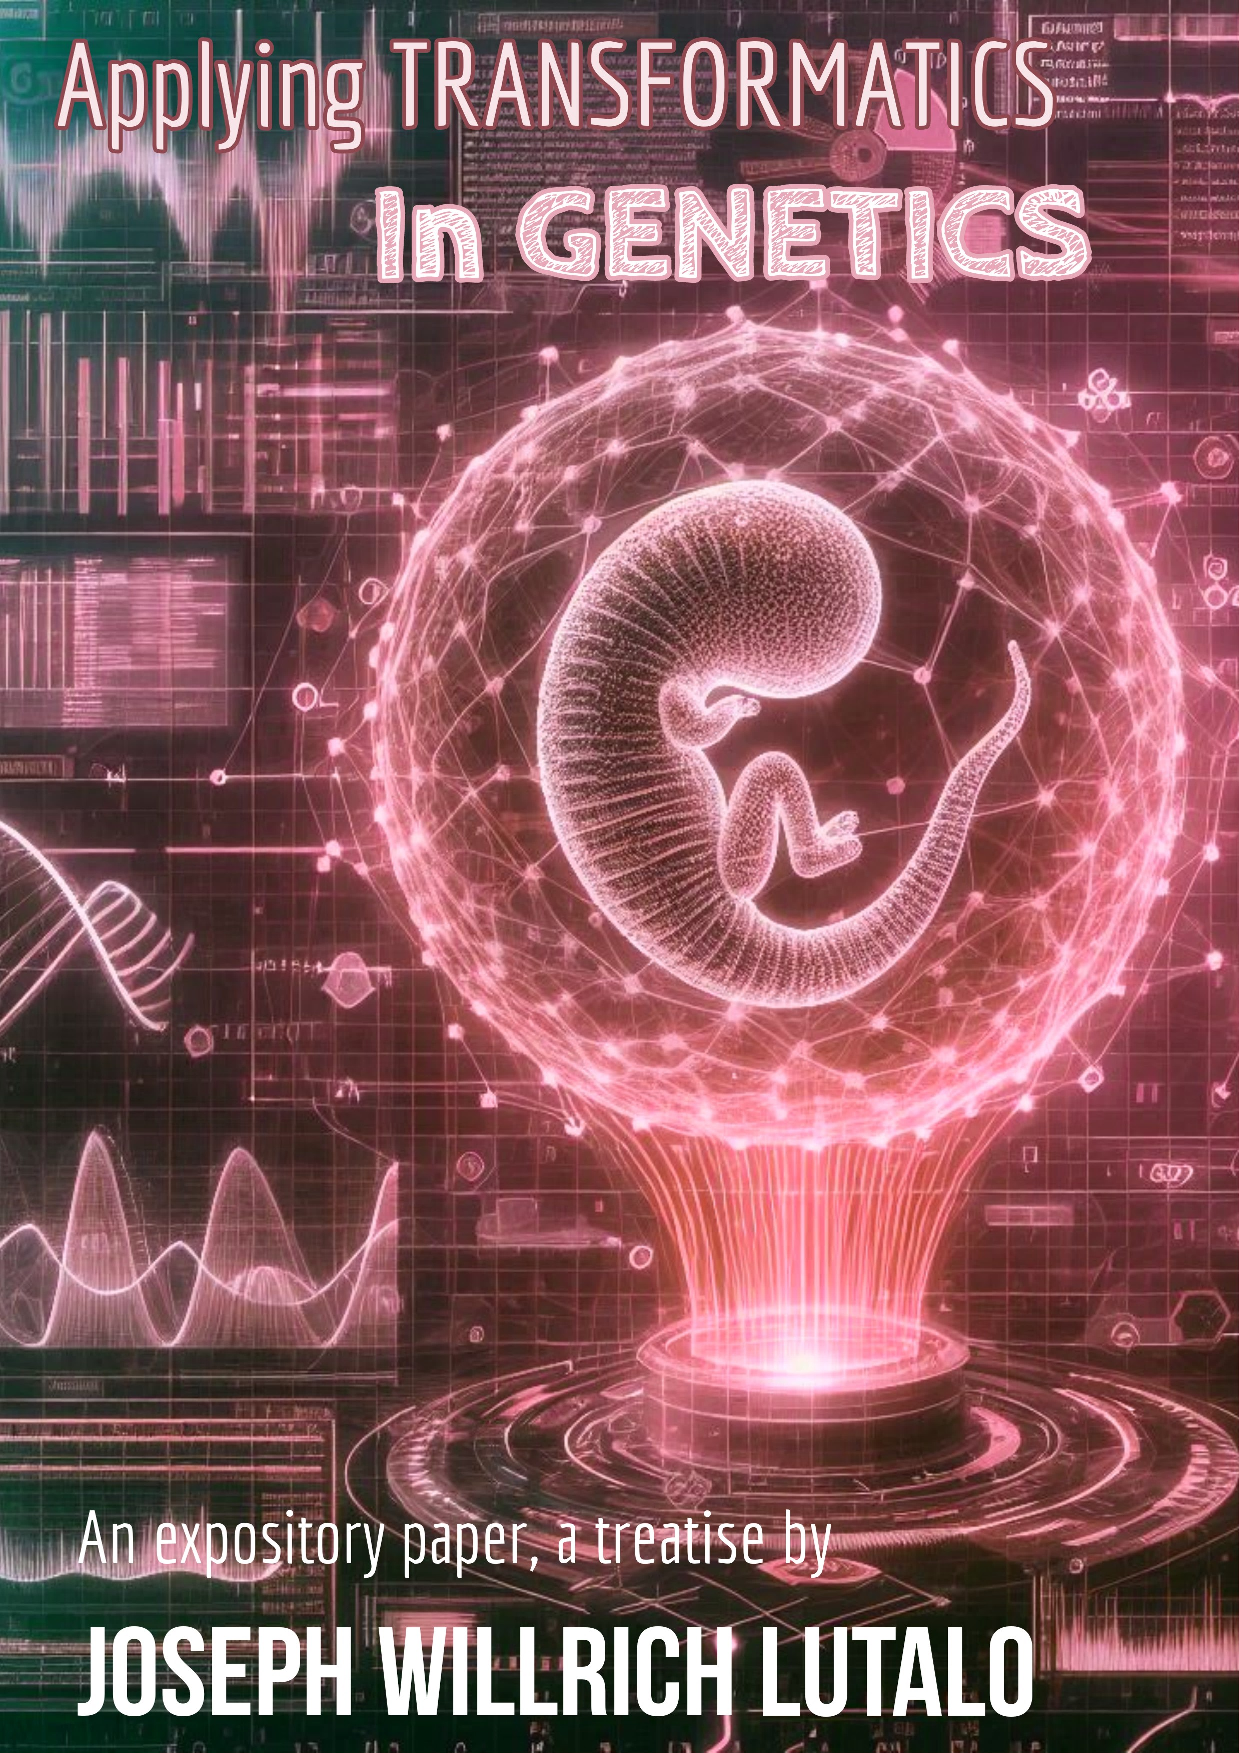
\includepdf[pages=1]{resources/pdfs/front_cover.pdf}


% insert I*POW frontmatter
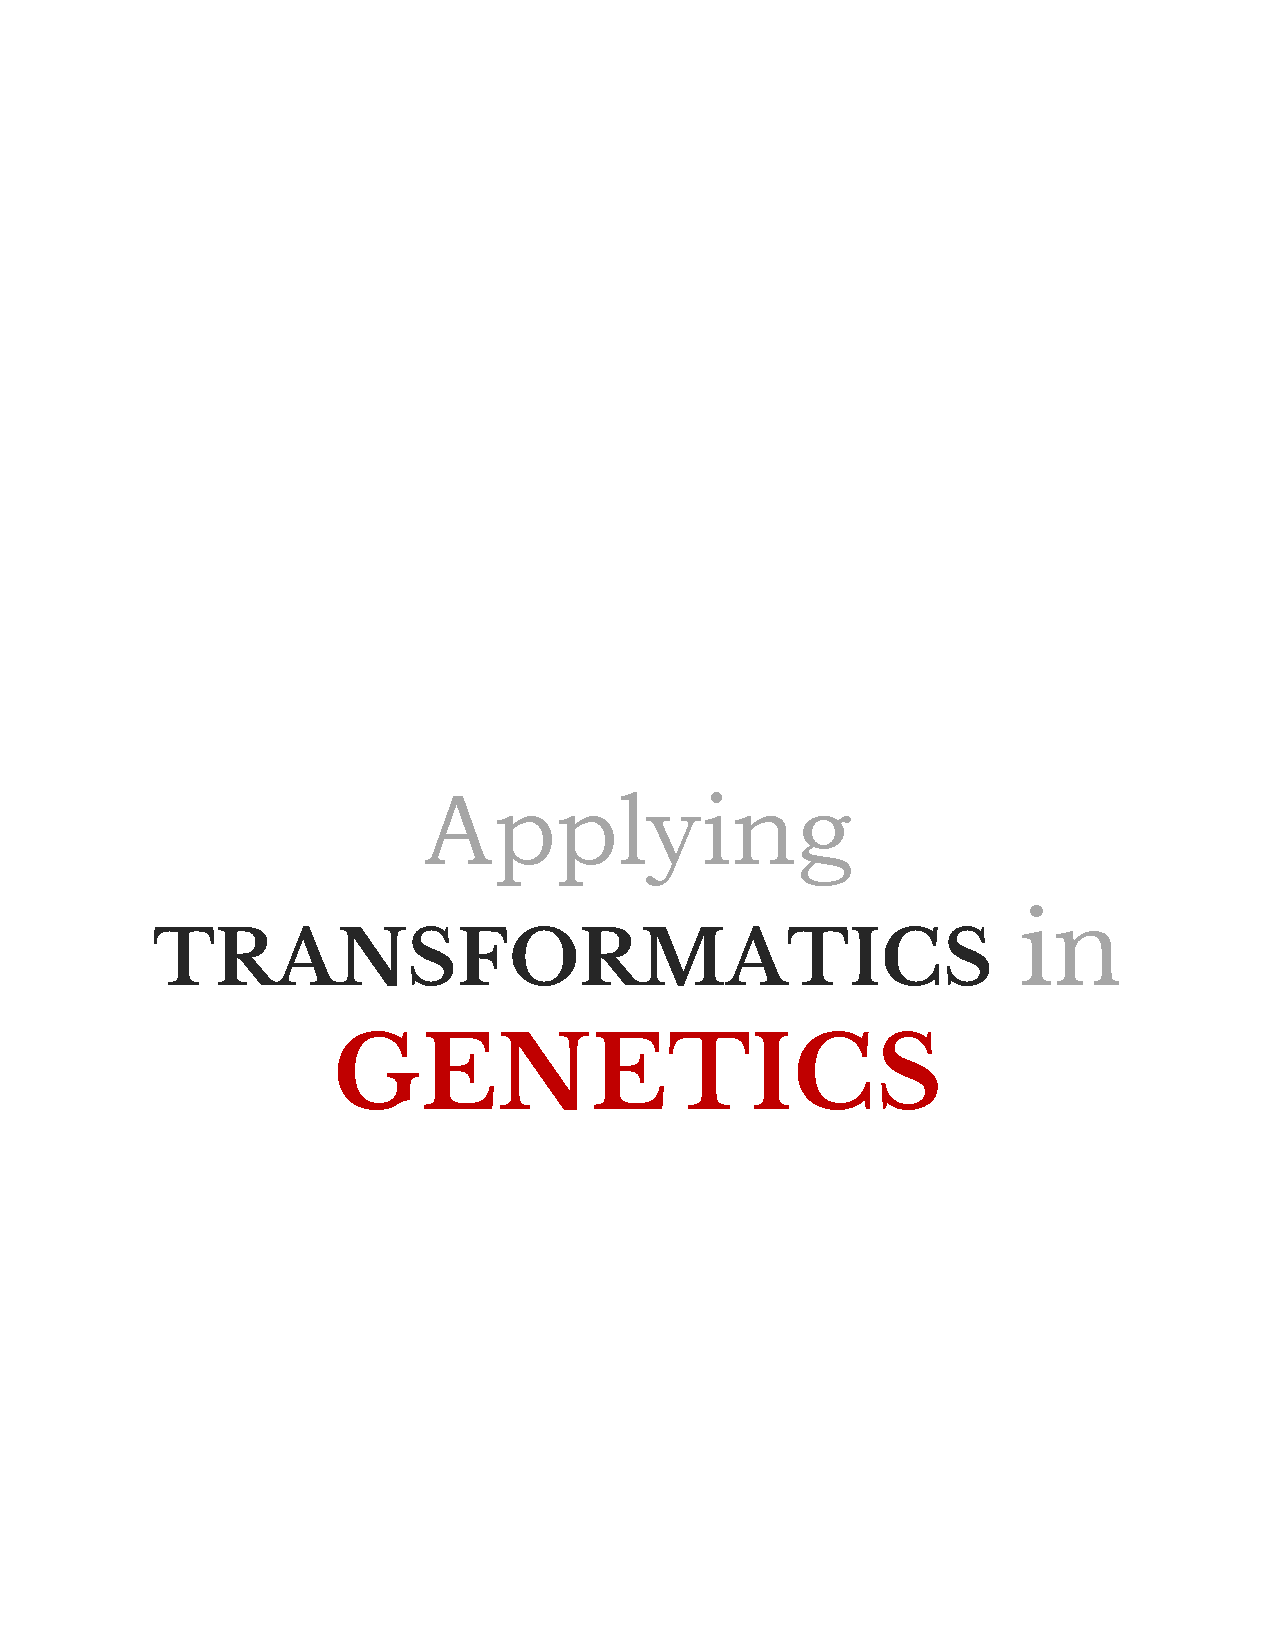
\includepdf[pages=-]{resources/pdfs/FrontisMatter.pdf}



\maketitle

\chapter*{Dedication}


\begin{table}[H]
  \centering
  \Huge
	\begin{tabular}[t]{|p{0.8\textwidth}}
The friendly, 20th century philosophical entertainer, \textbf{Alan Watts}, \normalsize such a fatherly, enlightening voice I keep hearing in my thoughts every once in a while; for I enjoy listening to his rants, once said \Huge \textit{``You are the universe experiencing itself."} \Large I always wished to be a father to someone... \textbf{a real boy or a girl out there... a soul... my own genetic code alive and existing independently of me}. To experience and enjoy the expressions of my own genetic code remains among my greatest dreams. But, in case I don't see my own child in this lifetime, at least, this message should inspire those that read it, who come after, to know and trust that when we express ourselves, we in a way express those that brought us into the world. Personally, I would cherish it! I surely dedicate this work to you, my father and mother. \Large I can't express enough how grateful I am, that you enabled me to be... You gave me a distinctive identity and a voice. \Huge \textbf{May this work help further your expressions in this world... and beyond.}\\
	\hline
	              
\end{tabular}
  \label{TABDEDC}
\end{table}

\tableofcontents

\listoffigures

\listoftables

\newpage

\Large


\chapter{Preface}
\label{SECPREFACE}


\vspace{2em}

\noindent
\begin{minipage}{1\textwidth}
\vspace{1em}
\begin{quotation}
\noindent {\ttfamily

Jung restored the \hl{colour} in science, and made me cherish the mind in new ways...\\

And that in exercising our will we might become aware of the divine in us and thus make glory manifest. God is not asleep in us!

}
\hspace*{\fill} --- \textbf{J. Willrich Lutalo}, \textit{Shrines of The Free Men}, 2018\cite{shrinesjwl}
\end{quotation}
\vspace{1em}
\end{minipage}

\vspace{2em}



We are living in a world where man affects and influences nature so much, especially with his \textit{unnatural} inventions in the form of animated and inanimate intelligence, implements and reality augmentations. But also, the world around man is constantly changing, and sometimes, in ways other than man is naturally comfortable with. That said, there is this idea that \textit{a life unexplored isn't worth living}\footnote{I trust, it is attributed to ancient philosopher and student of \textbf{Socrates}, Aristocles son of Ariston aka. `Plato'.}, and come what may, with every passing day, and as seasons and times change, it seems like the compulsion for humans to have to leave their traditional home environments and explore life elsewhere --- say, in foreign countries, in/under the sea, \textit{inside} the earth or away from it, say like in outer-space, etc. seems so unavoidable --- in fact, it feels to me like it is inculcated into our very natures, so that, thinking about a future in the same exact space, with the same exact people, environment and circumstances as we wake up to every day just doesn't make much sense\footnote{I have read a sane dose of \textbf{Daniel Defoe}'s classic, \textit{The Life and Adventures of Robinson Crusoe}, a relic from 1719, and among things Defoe seemed to argue against, was the somewhat strong urge in some humans, to want to go ``abroad upon Adventures, to rise by Enterprise, and make themselves famous in Undertakings of a Nature out of the common Road".}. That we must prepare ourselves --- ``we", meaning \textit{humans}, to face an uncertain future, but also, to lessen such uncertainty to manageable levels where possible or necessary, is much of what justifies our investments in and explorations of science and knowledge in general. 

For those who trust \textit{divinely inspired} wisdom\footnote{I keep an indispensable copy of \textbf{The New Jerusalem Bible}, and wouldn't wish to do much without consulting it first!}, the sacred scriptures (in \textbf{Genesis 1:28}) empower us thus:


\vspace{2em}

\noindent
\begin{minipage}{1\textwidth}
\vspace{1em}
\begin{quotation}
\noindent {\ttfamily

God blessed them, saying to them, \textit{Be \textbf{fruitful, multiply, fill the earth and subdue it}. Be masters of the fish of the sea, the birds of heaven and all the living creatures that move on earth.}

}
\end{quotation}
\vspace{1em}
\end{minipage}

\vspace{2em}


Despite not having been funded by any one or any particular organization, the author, passionate about his pursuit of a \textbf{Doctorate in Philosophy} --- of Computer Science or Mathematics, from the \textbf{University of Oxford}\cite{lutalo_2025_sop}\cite{Lutalo2025_phd} or any other reputable institution\footnote{Refer to \textbf{ORCID:} \url{https://orcid.org/0000-0002-0002-4657}}, and especially to secure a teaching or faculty position, somewhere\footnote{Because, in all fairness, knowledge must not only be sought or furthered, but must also be shared.}, embarked on this project, especially to further his earlier work on Transformatics\cite{transformatics} as well as to bring to better audiences, the now stable advances in his original, commercially-viable \textbf{TEA programming language}\cite{cli_tttt}, by exploring new ground, proposing ideas and applications, in a domain potentially more in-demand and with far-reaching consequences for not just humanity, but all of nature, now, tomorrow, and in the deep, far-future. 



% Title for the section
\chapter*{List of ACRONYMS}
\addcontentsline{toc}{chapter}{List of Abbreviations}
\label{CHAPACRONYMNS}

% Longtable for abbreviation list
\begin{longtable}{p{3cm} p{12cm}}
\textbf{ABBR.} & \textbf{Definition} \\
\hline
\endfirsthead

\textbf{ABBR.} & \textbf{Definition} \\
\hline
\endhead

% Add your abbreviations below
\textbf{ADM} & Anagram Distance Measure \\
\textbf{COS} & Consensus Overlapping Sequence \\
\textbf{DNA} & Deoxyribonucleic Acid \\
\textbf{FGE} & Full Genome Expression \\
\textbf{FLSA} & First Lu-Shuffle Algorithm \\
\textbf{IFA} & Intermediate Form Affix \\
\textbf{I*POW} & International Portfolio of Writers \\
\textbf{IGS} & Identity Genome Sequence \\
\textbf{JSON} & JavaScript Object Notation \\
\textbf{LGES} & Lu-Genome Expression System \\
\textbf{LNS} & Lu-Number System\\
\textbf{MCS} & Maximum Common Subsequence \\
\textbf{\textit{m}RNA} & \textit{messenger}-\textbf{RNA} \\
\textbf{MSS} & Model Sequence Statistic \\
\textbf{\textit{n}-SSI} & \textit{natural}-Symbol Set Identity \\
\textbf{\textit{o}-SSI} & \textit{orthogonal}-Symbol Set Identity \\
\textbf{ORS} & Overlap Resultant Sequence \\
\textbf{PFA} & Platonic Form Aspect \\
\textbf{RNA} & Ribonucleic Acid  \\
\textbf{RNG} & Random Number Generator  \\
\textbf{RPMSS} & Representative Population \textbf{MSS}  \\
\textbf{RSG} & Random Sequence Generator  \\
\textbf{SLSA} & Second Lu-Shuffle Algorithm  \\
\textbf{TEA} & Transforming Executable Alphabet \\
\textbf{\textit{t}RNA} & \textit{transfer}-\textbf{RNA} \\
\textbf{WSL} & Windows Subsystem for Linux\\
\textbf{x-LGES} & Extended \textbf{LGES} \\
\textbf{YAML} & Yet Another Markup Language \\


\end{longtable}




%---[ BEGIN BOOK CONTENT/CHAPTERS ]

\mainmatter

%\begin{abstract}
\chapter*{Abstract}
\large

It started out as just a paper but is now a treatise. \textbf{Applying TRANSFORMATICS in GENETICS} brings to surface the importance of leveraging the mathematical theory recently named ``Transformatics", that deals with the study, processing and analysis of especially sequences of symbols and their alteration via symbolic machines known as sequence transformers. In earlier and recent work by the author, it has been demonstrated to be a credible and powerful theory in designing, specifying and explaining the properties of automata operating on sequences to produce other sequences. In this particular work, we take that body of knowledge, as well as what we know about the important science of how biological life-forms are defined, transformed and expressed in nature based on genetic code sequences known as DNA (deoxyribonucleic acid), and use that to treat of old and new problems in the field of GENETICS, developing many new, and previously unpresented solutions based on the theories, calculus and mechanics of sequence transformers. We have used transformatics to develop, but also distill many useful general results in the form of theorems as well as 3 laws concerning na-Sequences. We have demonstrated how sequence transformers can be leveraged to solve specific practical problems in genetics via numerous well-structured sequence transformations. We have invented and presented several new algorithms that would allow the concepts and solutions we developed in transformatics theory for various general problems to be readily turned into computable solutions using any programming language, for scenarios in genetics, but especially via leveraging TEA and Python. We have demonstrated how to leverage statistical analysis to make quantifiable differences and similarities between two or more na-Sequences (including entire populations of them) readily discernible. Leveraging transformatics, we have developed a new theory and systematic framework, the Lu-Genome Expression System, with which, via explorations by eye and hand, but also via the use of computers, the matter of how individual DNA sequences, and generally, any sequence that can be transformed into a numeric/decimal sequence, can be used to explore the natural concept of gene and genome expression, in both a visual-spatial, but also mathematical-symbolic way. We have tackled the fundamentally critical problem of genome sequencing, and have managed to not only cast it rigorously using the language and formalisms of transformatics, but have also managed to define an abstract machine that can take a set of DNA sequences potentially out of alignment, and then derive from them, via systematic and meaningful alignment procedures, a final, representative consensus genome sequence. Though this work is significantly theoretical and mathematical, we anticipate that the discussions, notes, formulations, solutions and overall expository treatment of the subject that it brings forth, shall help inspire actual domain experts and other researchers interested in genetics, genetic engineering, and related sciences, to pick up and apply our transformatics theory and ideas in both theory and practice.
     \newline\newline
     \textbf{Keywords}: Mathematical Statistics, Linear Algebra, Transformatics, Artificial Intelligence, Sequence Processors, Sequence Analysis, DNA, Genetic Code, Genetic Analysis, Abstract Machines, Genome Sequencing, Genome Expression, Gene Programs, Transformers.
%\end{abstract}

\newpage

\chapter{Introduction}
\label{SEC1}


\begin{table}[H]
  \centering
  \begin{tabular}{|p{0.95\textwidth}} % Left border only
    \hline
    \begin{figure}[H]
      \centering
      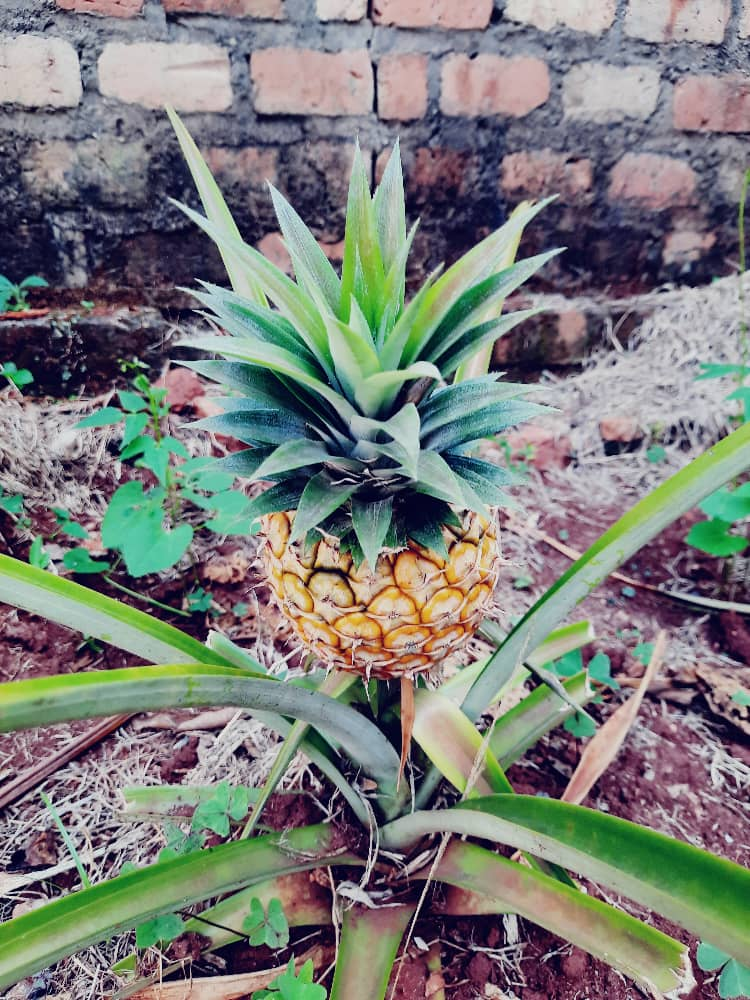
\includegraphics[height=0.6\textheight,]{resources/images/the_pineapple.jpg}\\
       \caption{In the course of writing this work, an experiment to grow pineapples from the pineapple fruit tops of pineapples normally bought from nearby marketplace (\textbf{Garuga/Bugabo-Bukaaya}) yielded results! Here we see the first successful harvest of a pineapple from our home garden (at \textbf{Nuchwezi Research}). But also, this case inspired part of the discussion in \textbf{\hyperref[SEC4]{Chapter \ref{SEC4}}} about how in real genome expression\index{genome expression} systems, the organism expressed from genetic code somewhat still includes the genetic code in the manifested organism as some kind of affix --- a prefix (in leaves for example) or suffix (roots), from which the original organism (or the same exact genome) might be later reproduced!}
      \label{FIGPINEAPPLE}
    \end{figure} \\
    \cline{1-1} % Bottom border only
  \end{tabular}
\end{table}


\vspace{2em}

\noindent
\begin{minipage}{1\textwidth}
\vspace{1em}
\begin{quotation}
\noindent {\ttfamily

Sex seems to have been invented around two billion years ago. Before then, new varieties of organisms could arise only from the accumulation of random mutations\index{mutations} --- the selection of changes, letter by letter, in the genetic instructions. Evolution must have been agonizingly slow. With the invention of sex\index{sex}, two organisms could exchange whole paragraphs, pages and books of their DNA code, producing new varieties ready for the sieve of selection. Organisms are selected to engage in sex --- the ones that find it uninteresting quickly become extinct. And this is true not only for the microbes of two billion years ago. We humans have a palpable devotion to exchanging segments of DNA today.

}
\hspace*{\fill} --- \textbf{Carl Sagan}, \textit{COSMOS}, 1981\cite{sagan1981cosmos}
\end{quotation}
\vspace{1em}
\end{minipage}


\vspace{2em}

\noindent
\begin{minipage}{1\textwidth}
\vspace{1em}
\begin{quotation}
\noindent {\ttfamily

The material basis of heredity is DNA\index{DNA}, a ladder-like molecule which carries a message in the form of a `four-letter' code, the letters being four chemical bases, each of which may occupy any rung in the ladder.

}
\hspace*{\fill} --- \textbf{The Oxford Companion to the Mind}\cite{gregory1987oxford}
\end{quotation}
\vspace{1em}
\end{minipage}


\vspace{2em}



In reality, we find that living, real organisms are influenced by genetics\index{genetics}, their environment, bits of randomness and sometimes emergent behaviors that might not be readily captured by strict rules such as the genetic code of life. However, away from all possibilities, and focusing on what can be said of life expression via the genetic code known as DNA (the \textit{deoxyribonucleic acid}\index{DNA!deoxyribonucleic acid}) and RNA\index{RNA} (\textit{ribonucleic acid}\index{RNA!ribonucleic acid}), especially when applied to the vast spectrum of natural organisms on earth --- from basic \textbf{prokaryotes}\index{prokaryotes} (single-celled organisms) such as the simple bacteria that actually have no nucleus\cite{bioexplorer2025}, to  \textbf{eukaryotes}\index{eukaryotes}; all the way from basic one-cell kinds such as amoeba\cite{kang2017deep} all the way to sophisticated creatures such as oak trees, vultures, dolphins and human beings! Talking of which, it might be important to set clear that though \textbf{viruses}\index{virus} are a kind of life-form\cite{libretexts2025viruses}, and yet, they are neither prokaryotes nor eukaryotes --- especially because, fundamentally, they are merely some genetic code (DNA or RNA) ``enclosed in a protein coat, lacking cell membranes or organelles"\cite{libretexts2025viruses} --- more technically they are \textbf{acellular entities}.

So, if we bring on-board ideas from \textbf{transformatics}\cite{transformatics}\cite{Lutalo2025_transformatics_thesis}\index{transformatics!genetics introduction} --- a new mathematical theory\footnote{Also, refer to the \textbf{appendix} --- particularly \textbf{\hyperref[CHAPTRANS]{Chapter \ref{CHAPTRANS}}}, which reproduces verbatim, the ``Transformatics 101" manuscript --- a \textit{mini-thesis} --- that serves as the authoritative introduction to and baseline justification for this new mathematical theory.} dealing with sequences of symbols or those of named structures and their processing as well as analysis; for example, if we take the transformatics theory concepts such as comparing sequences using new measures such as the Anagram Distance Measure (ADM), or perhaps leveraging the sequence summary measure known as the modal sequence statistic (MSS), and these then being applied to sequences such as DNA, we find that, independently of, and without needing to first consult or worry about mainstream genetic code analysis or genetic engineering theory and mechanics, that we can say many useful things about such genetic code sequences and that we might be able to break new ground or solve some otherwise still intractable problems concerning sequences of genetic code in general.



\begin{table}[H]
  \centering
  \begin{tabular}{p{0.95\textwidth}|} % Left border only
    \hline
    \begin{figure}[H]
      \centering
      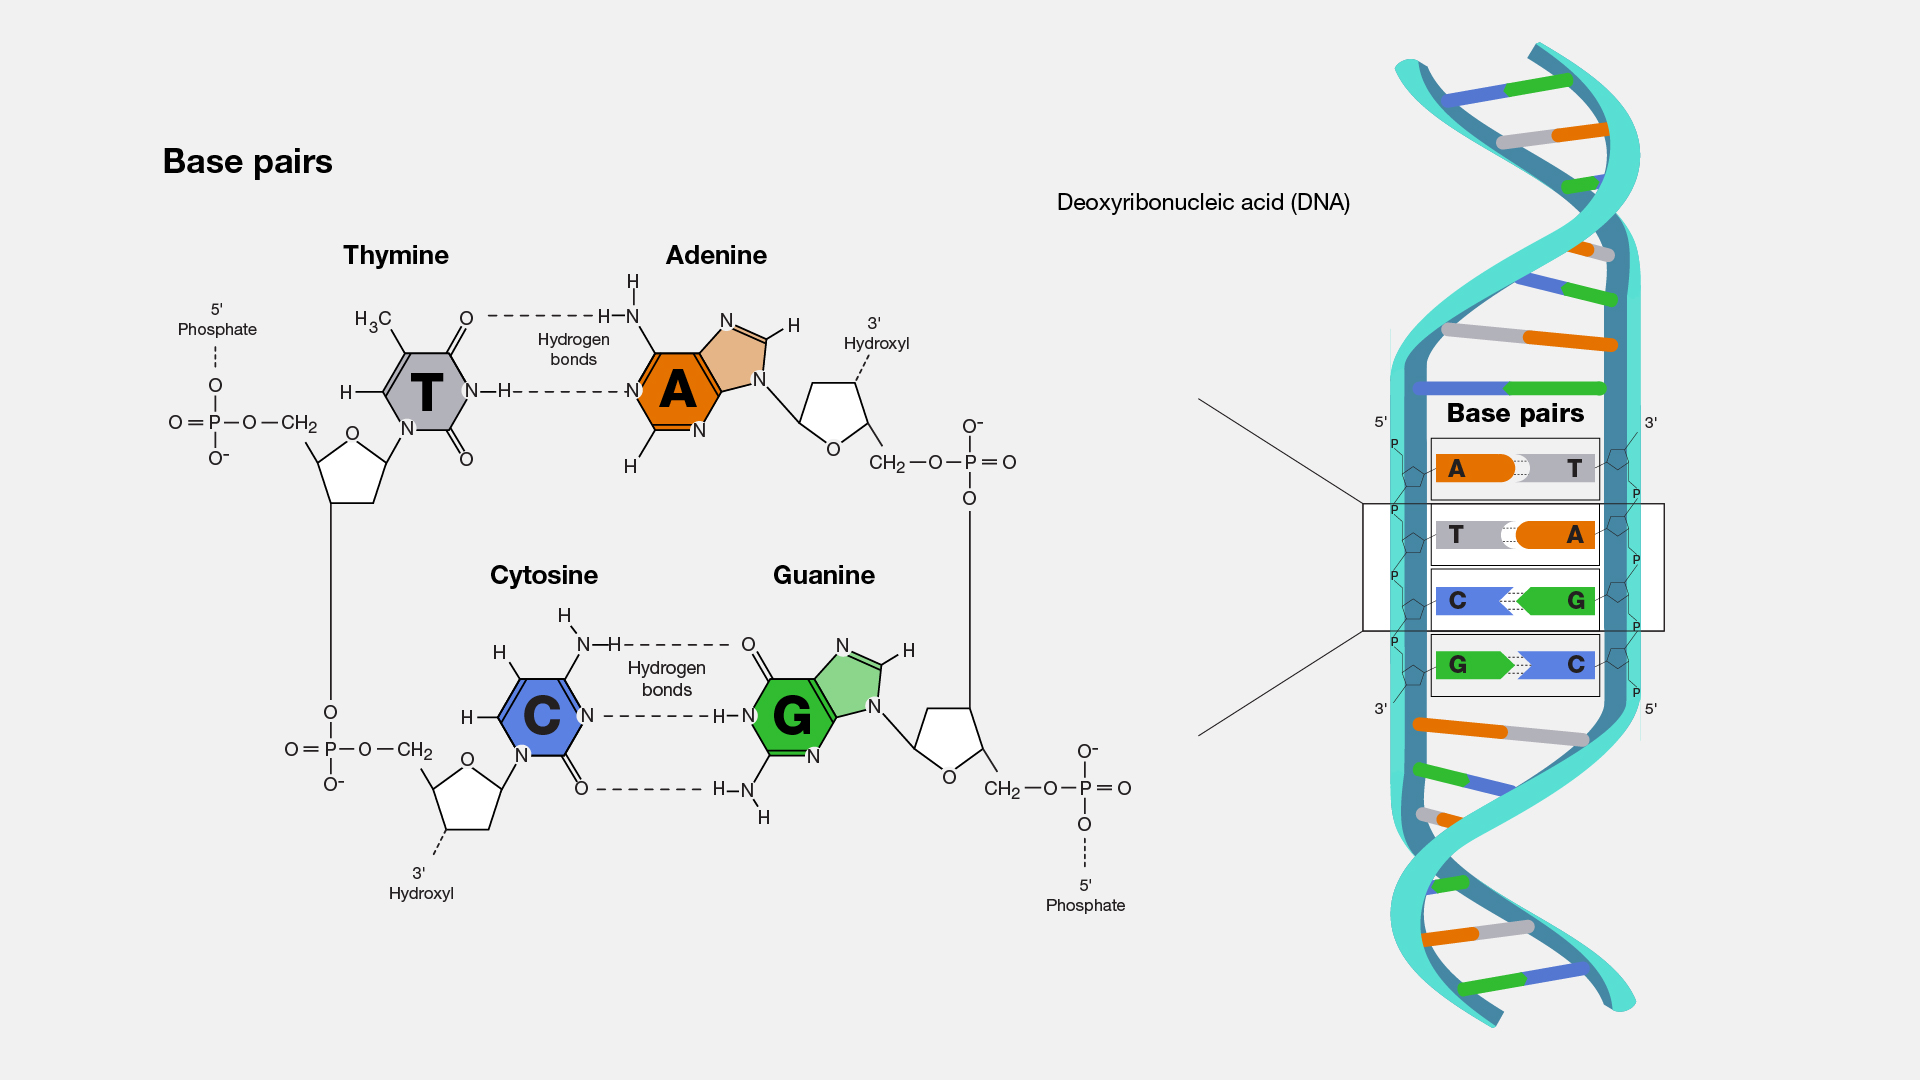
\includegraphics[width=0.9\textwidth]{resources/images/dna_diagram.jpg} \\
       \caption{A basic diagram of the chemical structure of DNA base-pairs, sourced from \cite{wikipedia_basepair}}
      \label{FIG1}
    \end{figure} \\
    \cline{1-1} % Bottom border only
  \end{tabular}
\end{table}
    


For example, by borrowing a useful DNA-as-library\index{DNA!library metaphor} metaphor from Venville et al\cite{venville2006analogies}, we would come to appreciate that by looking at \textit{DNA as a library of books}, we have a model such as:

\begin{enumerate}
\item \textbf{Library}: DNA (as a whole) --- the \textbf{Genome}\index{genome},	 as the complete collection of genomic data about an organism.
\item \textbf{Bookshelves}: \textbf{Chromosomes}\index{chromosomes} as organized storage of genes, and that they (chromosomes) are long, coiled-up strands of pairs of genes (essentially, the chromosome is a combination of two strands of genes, with one called the \textit{template} and the other a \textit{complement}, and that when they come together to form the ``ladder" structure, at each step, the two genes forming a step are paired such that $A \leftrightarrow T$ and $C \leftrightarrow G$ \cite{passel_dna_structure} --- also see \textbf{\hyperref[FIG1]{Figure \ref{FIG1}}}). So, for example, humans have 46 chromosomes in total in their ``DNA library" (23 chromosome pairs, consisting of 22 autosomal pairs plus one pair of sex chromosomes). We know that during reproduction, the [full] genome (46 chromosomes in humans) splits up by half in either parent (via \textit{meiosis}, which somewhat shuffles the complete genome and then halves it\cite{genomics2025origin}), so that only one-half of the otherwise well-paired template-complement set that is the chromosome strand from each parent (as either sperm or ovum) goes to contribute to the final chromosome collection-set of the offspring\cite{libretexts2025gametogenesis}\cite{gregory1987oxford}. Whereas, after fertilization or during normal cell division, the entire chromosome set (with well-paired strands) is duplicated/replicated wholesomely and losslessly so that the second/new cell thus created has an exact copy of the same chromosome set (entire genome) as was in the source cell\cite{leicester_cellcycle}. 
\item \textbf{Books}: The \textbf{Genes}\index{genes} which make up a chromosome are the books in our genome library. Each gene is essentially a collection of ``words" that are a sequence of one or more codons (see below), and which taken together, contain enough information/instructions to specify how to produce a specific protein\cite{gregory1987oxford}\cite{venville2006analogies}.
\item \textbf{Words}: And then, at the next, lower abstraction level than genes, we have \textbf{Codons}\index{codons}. These are like ``words" in each book, and each codon \textbf{only} codes for a single \textbf{amino acid}. Basically, a codon is a combination of any 3 of the ``letters" of genetic code, for which, there are exactly four for DNA (A, C, G, T) and four for RNA (A, C, G, U). We also know that there are at most, 64 possible unique combinations of the four letters into triplets/3-grams/the codons\cite{gregory1987oxford}.
\item \textbf{Letters}: Finally, at the most basic level of our genetic code/DNA-library/genome, we have ``letters" that are technically known as \textbf{nucleotides}\index{nucleotides}. Essentially, each nucleotide contains \textbf{a single nucleobase}\index{nucleobase}, with only one difference between DNA and RNA as such; for DNA: $\{A, C, G, T\}$, and for RNA: $\{A, C, G, U\}$ --- we have already come across the names of the four letters for the DNA, however, concerning that extra/new one, `U', specific to RNA, its name is ``Uracil".
\end{enumerate}


So, with that introduction clearing up much of the basic genetics nomenclature and concepts that I shall use in the rest of this work, we then dive into the meat of our undertaking as laid out in the next section.

\subsection{How to Navigate the Book}
\label{SECHOWTONAV}

\begin{center}
\fbox{\begin{minipage}{0.9\textwidth}
\LARGE
\textbf{This Book is \hyperref[SECHOWTONAV]{Navigable}:}\\

To ease and leverage meaningful cross-referencing across the chapters --- including extension materials in the \hyperref[APPOTHERFUNC]{appendix chapters}, there is substantial employment of \textbf{emboldened}, typed, named, numbered and \hyperref[SECHOWTONAV]{interactive}\footnote{Every such link, when encountered in the electronic or digital edition of this book, is \hyperref[SECHOWTONAV]{clickable}, and when clicked, shall automatically jump to the location in the book where that reference points. For paper-printed or non-interactive reading experiences, the type (in form of a guiding concept name: \textbf{Definition}, \textbf{Transformer}, \textbf{Theorem}, \textbf{Chapter},...) and a reference number (\textbf{1.2}, \textbf{B.3}, \textbf{8},...) can be combined to determine where it is in the book the referenced item is.} references across the book. For consistency and ease of navigation, note that where they occur in the text, such shall appear and behave as either this link to \textbf{\hyperref[CHAPACRONYMNS]{List of Acronymns}} or \textbf{\hyperref[TRANSFTELEP]{Transformer \ref{TRANSFTELEP}}}.

\vspace{1em}

Finally, note that the book does offer an alternative way to locate and navigate the text based on keywords and terms of importance --- there is an \textbf{\hyperref[CHAPINDEX]{Index}} at the end of the book, with which one can readily jump to sections in the book where a term or topic of interest is first introduced or is being discussed substantially. Concerning these, terms in the index aren't necessarily highlighted in the text, however, as with the interactive references mentioned above, for those reading the electronic version of this book, the index offers an interactive mechanism to quickly jump to sections where the term is being applied.

\end{minipage}}
\\
\end{center}

The necessary foundation concepts and nomenclature have been well introduced in \textbf{\hyperref[SEC1]{Chapter \ref{SEC1}}} --- the previous section.

In \textbf{\hyperref[SEC2]{Chapter \ref{SEC2}}} I shall formally define the DNA and RNA symbol sets, $\psi_{DNA}$ and $\psi_{RNA}$. We shall look at the matter of the difference between the ordering of terms in these mathematically-oriented sets, relative to the common-place \textbf{A-T-C-G} ordering typical in biological and especially genetics literature. I shall define the more universal $\psi_{na}$ that would help apply logic to both DNA and RNA sequences, and shall generalize all such sequences as \textbf{na-Sequences}.

In \textbf{\hyperref[SECSEQAB]{Chapter \ref{SECSEQAB}}} we shall look at the idea of using n-grams such as the meaningful na-Sequence nucleobase 3-grams (technically known as \textbf{codons}) to abstract away various nuances of the flat-structure DNA or RNA sequence whose length might sometimes shoot into the millions or billions for realistic complete genome sequences. In \textbf{\hyperref[SEC05]{Chapter \ref{SEC05}}} we shall further these ideas when looking at how to process na-Sequences at n-gram level such as in naming or identifying subsequences. We shall also see that such abstractions might help manage complexity and simplify formalisms or algorithms dealing with na-Sequences such as in the formalization of protein synthesis for natural or artificial automata via codon-processing ribosomes.


In \textbf{\hyperref[SEC3]{Chapter \ref{SEC3}}} we shall look at how we might leverage the basic concept of a symbol set to analyze arbitrary na-Sequences. We for example shall look at how to automatically generate special ordered symbol sets corresponding to individual na-Sequences under various bases --- DNA, RNA, na- or even sometimes lexically meaningful AZ($\psi_{az}$). We shall see how to define special symbol sets based on n-gram abstractions of na-Sequences, such as might help in logic with special na-Subsequences such as START and STOP codons.


In \textbf{\hyperref[SEC3A]{Chapter \ref{SEC3A}}} we then shall consider the interesting matter of \textbf{complement sequences} and \textbf{complement symbol sets}. We shall look at how to generate complements given a starting sequence or symbol set. We shall look into the interesting fact that complementing $\psi_{DNA}$ helps us arrive at the common \textbf{A-T-C-G} ordering of terms such as in $\dot{\psi}_{DNA}$. And though we might not use it immediately, we shall see that we might also talk of orthogonal symbol sets and orthogonal symbol set identities (o-SSI\cite{ossipaper}) in relation to na-Sequences and their complements.

In \textbf{\hyperref[SEC4A]{Chapter \ref{SEC4A}}} we shall dive into how to leverage the \textbf{ADM} and \textbf{MSS} to perform non-trivial sequence analyses. We shall utilize four scenarios starting with basic cases between two individual sequences of potentially unequal lengths, all the way to analyzing entire collections or populations based on their representative na-Sequences. We shall look at how to leverage the \textbf{TEA}\cite{Lutalo2024_taz}\cite{cli_tttt} text-oriented, sequence-transformer chaining paradigm GPL to conduct some of the essential analyses proposed, readily via the command-line but also via any web browser on any major operating system, and especially with DNA/RNA sequences of any size stored in basic text files or merely held in strings. We shall see that using the concept of the \textbf{modal sequence statistic}, whether applied to individual na-Sequences, collections of them or just sub-sequences of longer DNA or RNA strands, can help us leverage statistical summary information about a sequence that might otherwise not be easy to glean or leverage from trivial inspection of a sequence. In this chapter too, particularly in \textbf{\hyperref[SECPROXPOP]{Section \ref{SECPROXPOP}}}, we shall develop an algorithm that might be utilized in applying artificial statistical intelligence to the matter of sequence classification problems relating to labeled datasets. The closely related \textbf{\hyperref[SECSEQPROXSEQ]{Section \ref{SECSEQPROXSEQ}}} shall consider the matter of identifying the \textbf{closest-sequence} from a collection of na-Sequences when given a particular query na-Sequence. Finally, \textbf{\hyperref[SECSEQSTORAGE]{Section \ref{SECSEQSTORAGE}}} shall consider the important matter of \textbf{optimal database storage of na-Sequences} as is typically found in real-world systems such as those that do whole-genome sequencing or in gene-banks, etc. 

In \textbf{\hyperref[SECMATHSEQ]{Chapter \ref{SECMATHSEQ}}} we shall get into some deep mathematics around the critical problem of genome sequencing. We shall tackle the fundamental problem in genetics engineering by breaking it down into 3 major problems. \textbf{\hyperref[PROBG1]{Problem G1}} dealing with the matter of how to compute the longest common subsequence given any two sequences. \textbf{\hyperref[PROBG2]{Problem G2}} dealing with how, as happens during conventional genome sequencing, we have sections of two or more sequences that are not exactly the same, but which must be reduced to some \textbf{consensus sequence} that is most true to all the input/available disparate identifying sequences. And then in \textbf{\hyperref[SECCOMPGENSEQ]{Problem G3}}, we shall consider how to arrive at the final best consensus sequence that also unifies all the disparate input sequences originally provided, into a single sequence that is then the consensus genome sequence of the entity under analysis.


We shall then turn our attention to the matter of how genetic code is translated into actual living organisms in \textbf{\hyperref[SEC05]{Chapter \ref{SEC05}}}, focusing at the molecular level, and shall tackle the matter of the algorithm by which the most basic synthesis happens in a cell.


And then shall wrap up our core explorations in \textbf{\hyperref[SEC4]{Chapter \ref{SEC4}}}, from where we shall look at what results from actual processing of genome sequences or rather DNA code; the manifestation of some living thing, an organism or some aspect of it as specified in the underlying genetic code. We shall especially deal with minimal entities such as viruses and simple organelles. Most importantly though, we shall explore \textbf{genome expression} formally and conceptually so, with the assistance of a thought-experiment. A hypothetical genome-expression system --- which we shall refer to as the \textbf{Lu-Genome Expression System} (LGES) shall be presented, and all our explorations shall be based on it. \textbf{\hyperref[SECOZIN]{Section \ref{SECOZIN}}} shall deal with a visual encoding method that leverages a digit-cipher named \textbf{OZIN}\cite{lutalo_2025_grimlumtauto}, and which is to be used to express storage-level genetic code (in decimal/numeric form), it its \textbf{intermediate form} --- equivalent to DNA-to-mRNA transcription in living organisms. We shall finally turn attention to the final expression step --- equivalent to mRNA-to-Protein/Function translation in nature, in \textbf{\hyperref[SECGENEXPRE]{Section \ref{SECGENEXPRE}}}, and shall get to see yet another innovation in the form of a genetic-code-to-spatial-form encoding based on a cipher we shall call the \textbf{Platonic Form Cipher} (\textbf{\hyperref[SECPLATONIC]{Section \ref{SECPLATONIC}}}). The essential algorithm for how to perform genome expression all the way from storage code into the final organism is depicted in \textbf{\hyperref[ALGCOZINPLATO]{Algorithm \ref{ALGCOZINPLATO}}}, and we shall close with some examples of complete, though hypothetical, fully-expressed genomes in \textbf{\hyperref[SECFULLGES]{Section \ref{SECFULLGES}}}.

The overall conclusion of the book is presented in \textbf{\hyperref[CONC]{Chapter \ref{CONC}}}, where we shall especially find properly distilled \textbf{KPIs} --- metrics concerning what the major contributions of this work are --- in literature, in mathematics, in genetics, in computer science, in philosophy, the humanities and arts. That chapter too, in \textbf{\hyperref[SECFUTUREDIRECT]{Section \ref{SECFUTUREDIRECT}}}, also clearly outlines the major problems, concerns, issues and areas of future exploration and research that this book proposes or could not immediately resolve in the present edition, and which are then left as \textbf{future directions} or \textbf{future work} for the reader, the student, the author, as well as any other interested or concerned researcher.

Finally, there are a few extra materials that have been set aside in the appendix, and these either augment or support earlier chapters in the book. In particular, we shall find:

\begin{enumerate}
\item \textbf{\hyperref[APPOTHERFUNC]{Chapter \ref{APPOTHERFUNC}}} that covers 6 alternative functions that DNA plays in a living organism apart from protein synthesis which we mostly focus on in much of this book.

\item \textbf{\hyperref[APPOZIN]{Chapter \ref{APPOZIN}}} that offers insights into where and how the interesting \textbf{OZIN Cipher} that we use in the \textbf{LGES} came to be.

\item \textbf{\hyperref[SECIFAMSSPFMAPS]{Chapter \ref{SECIFAMSSPFMAPS}}} that covers the matter of how to compute \textbf{PFA}s for particular na-Sequences.

\item \textbf{\hyperref[SECALTPFGESA]{Chapter \ref{SECALTPFGESA}}} that preserves the original \textbf{PFA} construction algorithm as part of the \textbf{LGES} theory.

\item \textbf{\hyperref[CHAPTRANS]{Chapter \ref{CHAPTRANS}}} that presents the formal distillation of all the essential foundational results (10)  and proposed general [theoretical] applications (10) of transformatics, these being presented in this book for the first time, as a verbatim reprint of the material originally presented in the \textbf{``Transformatics 101 explained"} mini-thesis\cite{Lutalo2025_transformatics_thesis}.

\item \textbf{\hyperref[CHAPSITTRANS]{Chapter \ref{CHAPSITTRANS}}}, comprising of material and theorizing that comes a little later than the material originally in \cite{Lutalo2025_transformatics_thesis}, and which attempts, for the first time ever, to rigorously situate the newly proposed sub-field and theory of transformatics, in the grand spectrum of most of mathematics as well as applied mathematics.

\item \textbf{\hyperref[SECFUTDIRECT]{Chapter \ref{SECFUTDIRECT}}} that deviates from mere genetics, and demonstrates how Transformatics might be applied in any other mathematical science, with a focus on Physics and just one interesting problem - \textbf{teleportation} and \textbf{time travel}.

\end{enumerate}




\chapter{Sequence Symbol Sets and Sequence Transforms Applied to Genetic Code}
\label{SEC2}


\begin{center}
\fbox{\begin{minipage}{0.9\textwidth}
\large
\textbf{NOTE:}\\
 On \textbf{Potentially Similar Mathematics}: \textit{Frobenoids?} \\

Frobenioids\cite{mochizuki_frobenioids1}\index{transformatics!relation to frobenoids}, as introduced by \textbf{Prof. Shinichi Mochizuki}, offer a category-theoretic abstraction of arithmetic structures such as divisors and line bundles, encoding transformations via morphisms that resemble symbolic rewritings under algebraic constraints\cite{copilot_dna_assistant}. In spirit, they parallel the logic of sequence transformers (from transformatics\cite{transformatics}), which operate by mapping\index{mappings}\index{transformatics!mappings} one symbolic sequence to another through rule-based transformations constrained by set-theoretic, statistical or general mathematical logic. However, even though both systems might serve as structured environments for encoding and navigating symbolic changes across mathematical objects such as general sequences and sets, I just wanted to bring this up here, so students and researchers interested in our transformatics mathematics, and who wish to take the discussions and ideas I present in this work to even more advanced levels or in unconventional directions, to readily pick a leaf and comfortably proceed to do so\footnote{Also refer to \textbf{\hyperref[CHAPSITTRANS]{Chapter \ref{CHAPSITTRANS}}} for more material --- even more detailed --- concerning contrasting transformatics to several other existing fields of mathematics and [applied] mathematical theories.}.

\end{minipage}}
\\
\end{center}

For the purposes of appreciating transformatics from a genetics engineering or general genetics research perspective, it shall be important to note that, like in the original transformatics paper\cite{transformatics}, beginning by appreciating that whatever formalisms and mechanics we might develop or talk about concerning genetic code or rather DNA, had better begin with a realization that we can model DNA\index{DNA!as sequences} as merely an ordered set\footnote{This terminology to be used with precaution as we later clarify in \textbf{\hyperref[SECDEFSTRUCTURES]{Section \ref{SECDEFSTRUCTURES}}}, since for the case of collections of symbols such as DNA, not only does order matter, but also, and unlike standard sets, duplication of elements or members is allowed --- thus the preference for the more technically correct term; ``sequence" --- and unlike what some might find elsewhere, there is no need to stress that sequences are ordered sets by repeating ourselves when we say ``ordered sequences" instead of just ``sequence"!} --- essentially, ``a sequence" of symbols.\\


In the introduction (see \textbf{\hyperref[SEC1]{Chapter \ref{SEC1}}}), I have already called out both the names and symbols assigned to the most basic units of any genetic code; essentially, the \textit{nucleobases} (or rather, nucleotides). For purposes of simplifying our mathematical logic later on, we shall here neatly define what roles these units play in the grand scheme concerning DNA and RNA code. Basically, we shall want to define the symbol sets for any DNA sequence and the symbol set for any RNA sequence.\\

\fbox{\begin{minipage}{0.9\textwidth}
\large

\begin{defn}[The \textbf{DNA Symbol Set}\index{DNA!symbol set}, $\psi_{DNA}$]
\label{DEFDNASS}

For any possible sequence of standard \textit{deoxyribonucleic acid} (\textbf{DNA}) for any possible living organism, the distinct nucleic acid base units are known as nucleotides\cite{wikipedia_nucleic_acid}, and these are essentially and exactly only four\footnote{Actually, or rather, in general, for nucleic acid sequences, the bases are four for either DNA or RNA, but, there are also conventions that extend this set to 17 or more to cater for cases like where there might be ambiguity about what the exact nucleotide\index{nucleotides}\index{DNA!nucleotides} in a particular position might be\cite{wikipedia_nucleic_acid} --- possibly during automated inference or sequencing of DNA sequences.};
\begin{itemize}
\item Adenine(A)
\item Cytosine(C)
\item Guanine(G)
\item Thymine(T)
\end{itemize}
And these are mapped to their representative, distinct single-letter symbols as shown. Thus, any possible DNA sequence must always consist of only one or more of those elements and nothing else. Thus, we might sum this up, using the symbol set concept\cite{Lutalo2024gtnc} as applied to sequences\cite{transformatics} as such:

\vspace{1em}

\begin{equation}
\label{EQSSDNA}
\psi(DNA) = \{A, T, C, G\}
\end{equation}

\vspace{1em}

    \textbf{\hyperref[EQSSDNA]{Equation \ref{EQSSDNA}}} helps to appreciate the extra non-intuitive fact that the special ordering of DNA base symbols in the order A-T-C-G is what is conventionally accepted\cite{nature_atcg}\cite{wikipedia_nucleic_acid} or commonly found in most genetics literature\footnote{It shall be important to bring it out at this point, that, especially for non-domain experts --- people not trained in or normally practicing in genetics or related fields, that the common ordering of the nucleotides in the A-T-C-G ordering might seem unconventional or peculiar! For example, one might wonder, why are they not listed in their alphabetical order? So, for purposes of settings things clear for everyone, the author established\cite{copilot_dna_assistant}, concerning this matter, that: ``The order A, T, C, G isn't alphabetical, and yet it's the most commonly used sequence when referring to DNA bases." We further learn that, the order A-T-G-C reflects a mix of historical usage and bio-chemical structure; \textbf{base-pairing logic}\index{DNA!base-pairing} that the DNA's double-helix is stabilized by ``complementary base pairing" in which A pairs with T (via 2 hydrogen bonds), and C pairs with G (via 3 hydrogen bonds), so that listing A with its partner T and then C with G emphasizes this pairing symmetry\cite{copilot_dna_assistant}. Further, we learn that early molecular biology texts and sequencing protocols (especially post-Watson \& Crick, 1953) adopted this order to reflect the ``functional relationships" between bases. It became entrenched in educational materials, sequencing software, and databases. And lastly, that in visual and structural conventions --- such as in diagrams (see \textbf{Figure \ref{FIG1}}) and models, A–T and C–G are often shown side-by-side. Listing them in this order reinforces the \textbf{duality} of the DNA ladder's rungs\cite{copilot_dna_assistant}. Lastly, that though there is no single documented moment when this convention begun, that the A-T-C-G order likely solidified in the \textbf{1970s - 1980s} during the rise of \textbf{Sanger sequencing}\index{sequencing} (developed in the 1970s), GenBank and EMBL databases, and overall in textbooks and molecular biology curricula.}.

However, and especially because, for transformatics, we wish to work with an \textbf{ordered symbol set}\cite{ossipaper} and not just \textit{any possible symbol set} so that we can apply mathematical logic that respects the ordering of terms in any sequence\cite{transformatics}, we shall then assume a convention similar to how we might derive an ordered symbol set for a sequence of numbers in some base (the concept $\psi_\beta(\Theta)$ --- see \textbf{Definition 5} in \cite{ossipaper}), and given we are using Latin-Alphabet symbols (from $\psi_{az}$\cite{transformatics}) for $\psi_{DNA}$, we might as well better define the \textbf{Lexically Ordered DNA Symbol Set}, $\psi_{DNA}$\index{$\psi_{DNA}$} as such:

\vspace{1em}

\begin{equation}
\label{EQDNASS}
\psi_{DNA} = \psi_{az}(\psi(DNA)) = \langle A, C, G, T\rangle
\end{equation}

\vspace{1em}

For all practical purposes unless where we merely wish to emphasize adherence to the tradition of ordering the nucleotides by their pairing order, we shall essentially imply $\psi_{az}(\psi(DNA))$ or rather $\psi_{DNA}$ when we talk of the \textbf{DNA Symbol Set}.

\end{defn}

\end{minipage}}
\\



\fbox{\begin{minipage}{0.9\textwidth}
\large

\begin{defn}[The \textbf{RNA Symbol Set}\index{RNA!symbol set}, $\psi_{RNA}$]
\label{DEFRNASS}

For any possible sequence of standard \textit{ribonucleic acid} (\textbf{RNA}) for any possible living organism, the distinct nucleic acid base units are known as nucleotides\index{nucleotides}\index{RNA!nucleotides}, and these are essentially and exactly only four;
\begin{itemize}
\item Adenine(A)
\item Cytosine(C)
\item Guanine(G)
\item Uracil(U)
\end{itemize}
And these are mapped to their representative, distinct single-letter symbols as shown. Thus, any possible RNA sequence must always consist of only one or more of those elements and nothing else. Thus, we might sum this up, using the symbol set concept as applied to sequences as such:

\vspace{1em}

\begin{equation}
\label{EQSSRNA}
\psi(RNA) = \{A, U, C, G\}
\end{equation}

\vspace{1em}

    \textbf{\hyperref[EQSSRNA]{Equation \ref{EQSSRNA}}} helps to appreciate the traditional ordering of RNA base symbols in the order A-U-C-G reminiscent of the natural base-pairing order of DNA after it is translated into RNA (U merely replacing T)\cite{thoughtco_geneticcode}. And as with DNA, we shall want to have a proper, meaningful 
\textbf{ordered symbol set} for the RNA base symbols that we can later use in mathematical logic. Thus we shall equivalently define one for any standard RNA sequences as: 

\vspace{1em}

\begin{equation}
\label{EQRNASS}
\psi_{RNA} = \psi_{az}(\psi(RNA)) = \langle A, C, G, U\rangle
\end{equation}

\vspace{1em}

And for all practical purposes in this work as well as after, we shall essentially imply $\psi_{az}(\psi(RNA))$ or rather $\psi_{RNA}$\index{$\psi_{RNA}$} when we talk of the \textbf{RNA Symbol Set} or the \textbf{Lexically Ordered RNA Symbol Set}.

\end{defn}

\end{minipage}}
\\

\vspace{2em}


Now that we have $\psi_{DNA}$ and $\psi_{RNA}$ well defined, we might immediately apply them to their finest use here: defining and supporting the special symbol set, $\psi_{na}$, that would or could allow for several kinds of nucleic acid sequences --- such as DNA for code stored in chromosomes and mitochondria, various kinds of RNA (\textit{m}RNA, \textit{t}RNA,...) and even synthetic/artificial/conceptual and also \textbf{random nucleic acid sequences}, etc. using a single universal nucleic acid symbol set. Thus we define $\psi_{na}$ below:

\vspace{2em}


\begin{defn}[The \textit{\textbf{Universal Nucleic Acid Symbol Set}}, $\psi_{na}$\index{$\psi_{na}$}]
\label{DEFUNA}
The \textbf{Universal Nucleic Acid Symbol Set}, $\psi_{na}$, is the set combining the ordered symbol sets for DNA and RNA sequences, and thus is comprised of the symbolic elements $\{A, C, G, T, U \}$.
\end{defn}


We shall appreciate how relevant and important \textbf{\hyperref[DEFUNA]{Definition \ref{DEFUNA}}} is, by realizing that any nucleic acid sequence, $\Theta$, obeys the following law:\\


\fbox{\begin{minipage}{0.9\textwidth}
\large

\begin{law}[1 Universal \textbf{Nucleic Acid Identifier Symbol Set}: $\psi_{na}$]
\label{LAWNA}
 The \textit{universal} symbol set $\psi_{na}$ is spanned by any natural nucleic acid sequence $\Theta$.
\begin{proof}
$\psi_{na} = \psi_{DNA} \cup \psi_{RNA} = \langle A, C, G, T, U \rangle \quad \land \quad \forall \omega \in \Theta, \omega \in \psi_{DNA} \lor \omega \in \psi_{RNA}$.
\end{proof}
\end{law}

\end{minipage}}
\\\\


As with many kinds of sequences dealt with in transformatics, the possession of a particular symbol set, such as $\psi_{na}$, allows for the practical use of such a set to implement logic in systems that can operate on signal based on symbolic expressions of well ordered elements in sequences or sub-sequences. For this matter then, we shall likewise want to make formal, the concept of a \textbf{na-Sequence}\index{na-sequence}

\begin{defn}[The \textbf{$na-$Sequences} --- (D/R)-NA Sequences: $\Theta_{na}:\mathbb{N} \times \psi_{na}$]
\label{DEFNASEQ}

Any sequence of either DNA or RNA nucleotides, or both --- basically a sequence of nucleic acids, expressible as some sequence of symbols from $\psi_{na}$ is a \textbf{na-Sequence} and its symbol set is potentially a superset of both $\psi_{DNA}$ and $\psi_{RNA}$. Equivalently:

\vspace{1em}

\begin{equation}
\label{EQNASEQ}
\forall \Theta_{na} = \langle a_i, \rangle, \quad a_i \in \psi_{na} \implies a_i \in \psi_{DNA} \lor a_i \in \psi_{RNA}
\end{equation}

\end{defn}

\vspace{2em}


If it is not immediately clear what the significance of \textbf{\hyperref[DEFDNASS]{Defition \ref{DEFDNASS}}} is or why it's important to unambiguously define $\psi_{DNA}$ as well as the other basic formal symbol sets we have just formalized, then perhaps the mathematical discussions in later sections like \textbf{\hyperref[SEC3]{Chapter \ref{SEC3}}} and \textbf{\hyperref[SEC4]{Chapter \ref{SEC4}}} might help make this more obvious.

So, with those very essential definitions out of the way, we can begin to think of how we might appreciate and apply concepts from transformatics in genetics, in a clearer, straight forward manner.

For starters, we can certainly say that irrespective of how long or from where a particular DNA sequence, $\Theta_{DNA}$, originated from, once any sequence of data\index{data} (e.g unstructured or unprocessed raw genetic code sequence dump), a string (say a proprietary encoding of some DNA code), a name (say of a particular species of interest and whose actual/representative genome sequence is know) or even a number (an id of a genome sequence in some standard genome database, etc.) is mapped to standard
DNA sequence code, we shall know that any such transformation or mapping obeys the following theorem:

\vspace{2em}

\begin{theo}[$\psi_{DNA}$ as the alphabet underlying any DNA sequence]
\label{THEODNA}
For any sequence of DNA, $\Theta_{DNA}$, derived from some source sequence $\Theta$, irrespective of whether that source is itself a DNA sequence or not, we know that such an encoding or mapping, if it results in a valid DNA sequence $\Theta_{DNA}: \mathbb{N} \times \psi_{DNA}$, obeys the following general transformation:\\

\begin{trans}
\label{TRANSmDNA}
$\Theta \rightarrow \Theta_{DNA};$\\
$\forall a_{i \in [1,\invpi(\Theta_{DNA})]} \in \Theta_{DNA} \quad \exists \rho \in \psi_{DNA}: a_i = \rho, \quad \forall i \in \mathbb{N}$
\end{trans}

\begin{proof}
    Assume $\Theta_{DNA}$ contains some symbol $\alpha$ such that $\alpha \not\in \psi_{DNA}$, it would contradict \textbf{\hyperref[DEFDNASS]{Definition \ref{DEFDNASS}}} which clearly dictates the legitimate membership of any DNA sequence.
\end{proof}

\end{theo}

\vspace{2em}


And definitely, the equivalent truth for RNA sequences would likewise follow from \textbf{\hyperref[DEFRNASS]{Definition \ref{DEFRNASS}}}. So, we can then correctly tell that a sequence such as $\Theta_{insulin}$, which is the genetic code sequence defined as:\\


\fbox{\begin{minipage}{0.9\textwidth}
\large
%\begin{equation}
%\label{EQINSULIN}
\begin{multline}
\label{EQINSULIN}
\Theta_{insulin} =  \texttt{ATGGCCCTGTGGATGCGCCTCCTGCCCCTGCTGGCGCTGCTGGCCCTCTGGGGACC}\\
\texttt{CCAGCCGCAGCCTTTGTGAACCAACACCTGTGCGGCTCACACCTGGTGGAAGCTCTCTAC}\\
\texttt{CTAGTGTGCGGGGAACGAGGCTTCTTCTACACACCCAAGACCCGCCGGGAGGCAGAGGAC}\\
\texttt{CTGCAGGTGGGGCAGGTGGAGCTGGGCGGGGGCCCTGGTGCAGGCAGCCTGCAGCCCTTG}\\
\texttt{GCCCTGGAGGGGTCCCTGCAGAAGCGTGGCATTGTGGAACAATGCTGTACCAGCATCTGC}\\
\texttt{TCCCTCTACCAGCTGGAGAACTACTGCAACTAG}
\end{multline}
%\end{equation}
\end{minipage}}

\vspace{2em}

And which sequence\footnote{$\Theta_{insulin}$ as depicted here, is the short coding DNA sequence (CDS) for the human \textbf{INS} gene --- the part that gets transcribed into mRNA and translated by ribosomes into the insulin protein\cite{copilot_dna_assistant}}\index{DNA!sequence example}, despite having been obtained from an authority --- the \textbf{Leiden Open Variation Database (LOVD)}, which is based on NCBI's RefSeq data\cite{RefSeq}, might need to be verified by hand or with a critical eye, and that's where a law such as \textbf{Theorem \ref{THEODNA}} would come in handy. Also, note that, unlike common sequence notations we might see in this work or that we have encountered before, we wrote $\Theta_{insulin}$ in a manner somewhat more convenient for the kind of verbose sequence that any actual na-Sequence code generally is. The notation; without opening or closing brackets around the sequence terms and neither commas betwixt them --- reminiscent of the \textit{String [Chart] Sequence} notation\index{sequence!string notation} we developed recently (see \textbf{Transformation 15} in \cite{transformatics}).

We might for example start to wonder, how might we go about determining if some two DNA sequences, $\Theta_1$ and $\Theta_2$ are the same or perhaps if they share parts of each other, and by how much? We might wonder if they are the same sequence merely shuffled/anagrammatized --- since we saw that this can occur during natural processes such as meiosis\cite{genomics2025origin}. In case they are different, we might want to for example quantify the relative frequency of their distinct members, e.g mapping $\psi_{DNA}$ or $\psi_{RNA}$ to a sequence of relative frequencies, etc. These are all things we shall soon look into and know very well how to do or talk about, using genetics terms and the mathematical language and techniques from transformatics in the rest of this book.

\chapter{Sequence Abstraction using Symbol Sets: From Flat-Structure Sequences to Higher-Order Sequences}
\label{SECSEQAB}


Especially for nucleic acid sequences, but also for any other kind of sequence $\Theta$, there might be legitimate situations in which looking at or dealing with the flat-structure sequence\index{sequence!flat-structure} --- such as for the actually modest\footnote{`Modest' because, genomes and realistic genome sequences can typically span millions of genes or billions of nucleotides. We for example know that for a typical human cell's DNA there are $\approx$3.2 billion base pairs\cite{Venter2001}, and yet we know each base pair consists of two nucleotides, one for each strand of the double-helix (so that's $\approx$6.4 billion), plus a few more ($\approx$16,569 base pairs) from mitochondrial DNA\cite{Anderson1981}} $\Theta_{insulin}$ (refer to \textbf{\hyperref[EQINSULIN]{Equation \ref{EQINSULIN}}}), might be cumbersome, ineffective or unnecessary. And so, we are going to briefly look at ways that we might re-write verbose flat-sequences in more terse or higher-order \textbf{abstract ways} so as to focus on details that the flat-structure perhaps doesn't clearly express. This for example is naturally relevant in the processing of say nucleic acid sequences --- since such is useful in scenarios where the processing of any such sequence is done in \textit{non-unity} \textbf{n-tuples} or \textbf{n-grams} --- such as with codons\index{codons} (nucleotide 3-grams) or as gene programs\index{gene programs} (self-contained protein synthesis or function-gene-program sequences composed using codons)\footnote{
For purposes of re-using this relevant concept, we shall here define: 

\begin{defn}[A \textbf{gene program}]
\label{DEFGENPROG}
 In the domain of NA-processors, a \textbf{gene program}, $\mathbb{G}_{p}$ is any sequence of na-Sequence symbols, such that the sequence expresses or contains some sufficient instructions in form of genetic code, that specify what to do, and nothing else --- this might for example be what protein or material to produce, or what DNA-driven function to perform --- the protein is basically an effect, based on just the contents of the sequence --- and nothing more, such that for any such sequence, its basic signature is $\mathbb{G}_{p}: \mathbb{N} \times \psi_{na}:p=\invpi(\mathbb{G}_{p})$.
$\qed$
\end{defn} We shall find ways to leverage this definition to express formalisms about how living things and their properties or traits are driven by such computable, affectant and ``well-ordered" sequences in the future. For example, a philosophy that all existence is but a composition of effects resulting from the processing of a basic genetic code:

\begin{trans}
\label{TRANSTOENASEQ}
$\mathbb{G}_{p}  \quad \xrightarrow{O_{process}} \quad \prod \text{Effect}_{i \in \mathbb{N}}  \quad \xrightarrow{O_{compose}}  \quad \text{Existence}$
\end{trans}

}, etc.

So, assuming we have some sequence of $n$ symbols $\Theta_1$ defined as such:

\vspace{1em}

\begin{equation}
\label{EQSEQ1}
\Theta_1 = \langle a_1, a_2,...,a_n\rangle
\end{equation}

\vspace{1em}

If we wish to re-write the same sequence such that every $k$ terms are grouped in the same subsequence, we can then re-write $\Theta_1$ differently as such:

\vspace{1em}


\begin{equation}
\label{EQSEQ2}
\Theta_1 \equiv \Theta_2 = \Theta_2(n,k) = \langle a_{11}, a_{12}, a_{13}, a_{1k}, a_{21}, a_{22},...,a_{(i)(k)},...,a_{(\frac{n}{k})(k-1)},a_{(\frac{n}{k})(k)}\rangle
\end{equation}

\vspace{1em}

Of course, in \textbf{\hyperref[EQSEQ2]{Equation \ref{EQSEQ2}}} we have somewhat wanted to extrapolate well and illustratively, what would happen in an informative case such as when $k = 4$ and $n$ is not only significantly larger than $k$, but is also its perfect multiple. Otherwise, we might more concisely write that same sequence generalization as:

\vspace{1em}


\begin{equation}
\label{EQSEQ3}
\Theta(n,k) = \langle \langle a_1, a_2, a_3, a_4 \rangle_1, \langle a_5, a_6,...,a_8 \rangle_2,... , \langle a_{(n-k)},...,a_{(n-k+k-1)},a_{(n-k+k)}\rangle_{\frac{n}{k}} \rangle
\end{equation}

\vspace{1em}

So, this expression in \textbf{\hyperref[EQSEQ3]{Equation \ref{EQSEQ3}}} is our first proper appreciation of what higher-order sequences\index{sequence!higher-order} might be like when they are an abstraction of normal flat-structure sequences. We see for example here, that the $k=4$ \textbf{bundling-parameter} means we shall process the original flat sequence\footnote{Note that we might also refer to a ``flat sequence" as a \textit{first-order} sequence.\index{flat sequence}\index{first-order sequence}} $k$ items at a time, and so, each subsequence in $\Theta_2(n,4)$ then contains exactly (or at most) 4 items --- we are assuming 4 is a factor of n to keep things simple. And so, we expect that, in total, we should have $\frac{n}{k}$ subsequences after applying the bundling transform:

\vspace{1em}

\begin{transf}[The \textbf{k-GRAM Generator}\index{generator}\index{generator!k- or n-gram generator}]
\label{TRANSFBUND}
$\Theta = \langle a_1, a_2,...,a_n\rangle \quad \xrightarrow{O_{bundle-k}(\cdot)} \quad \Theta^* \quad;$\\
$\Theta^* = \langle \langle a_1, a_2,..., a_k \rangle_1, \langle a_{k+1},...,a_{2k} \rangle_2,... , \langle a_{(n-k+1)},...,a_{(n-k+k-1)},a_{(n-k+k)}\rangle_{\frac{n}{k}} \rangle$\\
$\forall a_i \in \Theta \quad \exists a_{ij} \in \Theta^*: a_i = a_{ij} \quad \land \quad j \in [1,k]$\\
For some $n, k \in \mathbb{N}$, and that $\invpi(\Theta^*) = \frac{n}{k} = $ number of k-gram subsequences generated from $\Theta$. $\qed$
\end{transf}

\vspace{1em}


Thus, we see that the sequence depicted in \textbf{\hyperref[EQSEQ3]{Equation \ref{EQSEQ3}}} with $k=4$ could as well be produced by the generator defined in \textbf{\hyperref[TRANSFBUND]{Transformer \ref{TRANSFBUND}}}. But not just that, if we applied that transformer to the DNA sequence $\Theta_{insulin}$ first presented in \textbf{\hyperref[SEC2]{Chapter \ref{SEC2}}} --- see \textbf{\hyperref[EQINSULIN]{Equation \ref{EQINSULIN}}}, we can then produce a proper standard codon/3-gram mapping of that DNA sequence that would look something like:\\


\fbox{\begin{minipage}{0.9\textwidth}
\large
%\begin{equation}
%\label{EQINSULIN}
\begin{multline}
\label{EQINSUL2}
\Theta_{insulin} \xrightarrow{O_{bundle-3}(\cdot)}  \langle \texttt{<ATG>,<GCC>,<CTG>,<TGG>,<ATG>,<CGC>,<CTC>,...,<ACC>}\\
\texttt{...,<TAC>,<TGC>,<AAC>,<TAG>} \rangle
\end{multline}
%\end{equation}
\end{minipage}}
\\\\

And the way we have bundled up the nucleotides in \textbf{\hyperref[DEFRIBOSOME]{Definition \ref{DEFRIBOSOME}}}, \textbf{\hyperref[EQ7]{Equation \ref{EQ7}}} is exactly how a natural sequence processor such as a Ribosome (see details in \textbf{\hyperref[TRANSF3]{Transformer \ref{TRANSF3}}}) would process it so as to produce say the corresponding protein.

Of course, though we might not delve into it here or at the moment, we know that by chaining several sequence transformers --- such that one operates on the output of the previous one to produce the next sequence (see \textbf{\hyperref[TRANSTOENASEQ]{Transformation \ref{TRANSTOENASEQ}}} as an example), we can arrive at even higher abstraction sequences that might render certain sequence processing programs easier to write, analyze or define. For example, we know that, much as a Ribosome Processor operates on a sequence of codons, and yet, any legitimate protein synthesis and genetic code sequence processing program will require some sort of necessary delimiters (such as the START and STOP codons --- refer to the Protein Synthesis Flow Chart in \textbf{\hyperref[FIG3]{Figure \ref{FIG3}}}), and so that, we might (if we could), abstract away codons and instead generate from a flat-structure DNA or perhaps mRNA sequence, a higher-order n-gram sequence of genes or \textbf{gene-program sequences}\footnote{We have defined gene programs in \textbf{\hyperref[DEFGENPROG]{Definition \ref{DEFGENPROG}}}.}\index{sequence!gene-program}.


\chapter{Sequence Analysis Using Symbol Sets}
\label{SEC3}


We now turn our attention to the matter of using ideas from transformatics to help analyze or understand genetic code sequences. For starters, we shall want to consider the matter of how to tell how far apart or dissimilar any two nucleic acid sequences might be. Of course, consequently, that would also translate into meaningful ways to tell how far apart not just low-level genetic-creations such as tissue, various cell-types, proteins, etc. might be based on the genetic code that specifies them, but also how different entire organisms --- made up of all these things, and within the same species or not, might be\footnote{So that then, we perhaps can also talk of \textit{genome analysis}\index{genome!analysis}.}.

Because we can learn much about an organism based on its characteristic genome, and since that can be mapped to a flat-structure sequence of symbols such as we have already encountered in earlier sections, it might start to make sense to leverage the similarity/distance measures we have already developed so as to apply them to quantifying the \textit{formal distance} between say actually different species. 

In an earlier paper\cite{adtpaper}, we have introduced and also demonstrated how a sequence-analysis measure called the \textbf{Anagram Distance Measure}\index{ADM}\index{sequence analysis!anagram distance}, $\tilde{A}(\Theta,\Theta^*)$, might be used to quantify how far apart some two sequences $\Theta$ and $\Theta^*$, that for the simplest scenarios better be of the same length, can be compared based on their common membership and the relative lexical ordering of the members in either sequence.

In the basic analysis we shall use to illustrate or develop our analytic concepts, we shall deal with hypothetical nucleic acid sequences mostly --- especially DNA sequences, and their lengths shall be kept short to keep our analyses simple. Moreover, their membership or composition --- in terms of nucleotides, might have nothing to do with actual/natural na-Sequences out there in the wild. The concepts and ideas we shall develop though, despite how we are going to develop them, should still be readily applicable to any or most nucleic acid sequences if not any kind of sequences in general.


\section{Testing Sequences for Membership in a Base}

First, assume we have the following three sequences\index{sequence analysis!base membership}

\begin{enumerate}
\item $\Theta_1 = CATGGGACTGCC$
\item $\Theta_2 = ATAATAAGAGGGATCTGA$
\item $\Theta_3 = AUAGGGAGAAUC$
\end{enumerate}

We can start by attempting to answer the question: \textbf{Which of these sequences are DNA and which are RNA?}

So, to answer that question properly --- \textit{provably} so, we can start by reducing each of those sequences to their respective [ordered] sequence symbol sets. In fact, if we first relax the assumption that they are either DNA or RNA sequences, and merely look at them as though they were any kind of sequence (for which we don't know the base or base-symbol set yet), then we can merely use the definition of an \textbf{Unspecific Symbol Set of $\Theta$ in Any Base}\index{symbol set!unspecific} --- see \textbf{Definition 4} in \cite{ossipaper}. The algorithm for how to do that is simple and is well presented in that definition --- we basically create another sequence, in which we insert each distinct symbol from $\Theta$ that we encounter while processing the sequence from Left-to-Right\footnote{Such that the leftmost term is the first to be processed.}. Thus, we might construct the relevant transformer for this as such:

\vspace{1em}

\begin{transf}[\textbf{Sequence Unspecified Symbol Set Generator}\index{generator!unspecific symbol set}]
\label{TRANSSSGEN}$ $\\
$\Theta \xrightarrow{O_{suss-gen}(\cdot)} \Theta^* \quad;\quad \invpi(\Theta^*) \leq \invpi(\Theta) \quad \land \quad \Theta^* = \hat{\psi}(\Theta)$
\end{transf}

\vspace{1em}

And thus, applying that transformer\footnote{Please, be careful with \textbf{\hyperref[TRANSSSGEN]{Transformer \ref{TRANSSSGEN}}} --- in particular, note that, the special notation employed for the unspecific symbol set, $\hat{\psi}(\Theta)$, shouldn't be confused with that of the somewhat related, though entirely different notation and notion of an unspecific symbol-set's modal sequence, $\overset{>}{\hat{\psi}(\Theta)}$ or the modal sequence statistic of a sequence's symbol set,  $\overset{>}{\psi(\Theta)}$. Refer to \textbf{\hyperref[CHAPTRANS]{Chapter \ref{CHAPTRANS}}} for more on these other concepts.} to the three sequences we have, we shall obtain the following results:

\vspace{1em}

\begin{trans}
$\Theta_1 \xrightarrow{O_{suss-gen}(\cdot)} \langle C, A, T, G \rangle = \hat{\psi}(\Theta_1)$
\end{trans}

\begin{trans}
$\Theta_2 \xrightarrow{O_{suss-gen}(\cdot)} \langle A, T, G, C \rangle = \hat{\psi}(\Theta_2)$
\end{trans}

\begin{trans}
$\Theta_3 \xrightarrow{O_{suss-gen}(\cdot)} \langle A, U, G, C \rangle = \hat{\psi}(\Theta_3)$
\end{trans}

\vspace{1em}

At this juncture, we then can more closely inspect the original/source sequences via these special resultant sequences --- each of them a kind of symbol set, and then judge which of $\psi_{DNA}$ or $\psi_{RNA}$ they are best associated with. To proceed in a rigorous manner, we might also want to compute the \textbf{Natural Symbol Set of $\Theta$ in some Base-$\beta$}\index{symbol set!natural} --- see \textbf{Definition 5} in \cite{ossipaper}. A suitable transformer to compute such a symbol-set (for which, unlike the unspecific symbol set, orders the terms in the resultant sequence by their natural order of occurrence in the base's ordered symbol set) would be as such:

\vspace{1em}

\begin{transf}[\textbf{Sequence $\beta$-Natural Symbol Set Generator}\index{generator!natural symbol set}]
\label{TRANSNSGEN}$ $\\
$\Theta \xrightarrow{O_{snss-gen-\beta}(\cdot)} \Theta^* \quad;\quad \invpi(\Theta^*) \leq \invpi(\Theta) \quad \land \quad \Theta^* = \psi_\beta(\Theta)$
\end{transf}

\vspace{1em}

And, since we already have an idea what the symbol sets for each of the three sequences are --- from which we can guess and also disqualify some candidate bases --- e.g, since $\hat{\psi}(\Theta_3) \setminus \psi_{DNA} = \{U\}$, then $\Theta_3$ can't be a DNA sequence. However, to complete our analysis, note that:

\vspace{1em}

\begin{trans}
$\Theta_1 \xrightarrow{O_{snss-gen-DNA}(\cdot)} \langle A, C, G, T \rangle = \psi_{DNA}(\Theta_1)$
\end{trans}

\begin{trans}
$\Theta_2 \xrightarrow{O_{snss-gen-DNA}(\cdot)} \langle A, C, G, T \rangle = \psi_{DNA}(\Theta_2)$
\end{trans}

\begin{trans}
$\Theta_3 \xrightarrow{O_{snss-gen-RNA}(\cdot)} \langle A, C, G, U \rangle = \psi_{RNA}(\Theta_3)$\\
\end{trans}

\vspace{1em}

So, we can safely conclude that:

\begin{enumerate}
\item Since $\psi_{DNA}(\Theta_1) = \psi_{DNA}$, then $\Theta_1$ is a DNA sequence.
\item Since $\psi_{DNA}(\Theta_2) = \psi_{DNA}$, then $\Theta_2$ is a DNA sequence.
\item Since $\psi_{RNA}(\Theta_3) = \psi_{RNA}$, then $\Theta_3$ is a RNA sequence.
\item Even if we forced it, note that, $\psi_{RNA}(\Theta_1) = \langle A, C, G, T \rangle \neq \psi_{RNA}$, or rather that $\hat{\psi}(\Theta_1) \setminus \psi_{RNA} = \{T\}$ so $\Theta_1$ can't be an RNA sequence.
\end{enumerate} 

Talking of which, in case we had some variation of $\Theta_1$ that has no instances of T in it, such as the sequence $\Theta_4 = CAAGGGACAGCC$, then we shall find that:

\vspace{1em}

\begin{trans}
$\Theta_4 \xrightarrow{O_{suss-gen}(\cdot)} \langle C, A, G \rangle$
\end{trans}

\vspace{1em}

and that:

\vspace{1em}

\begin{trans}
$\Theta_4 \xrightarrow{O_{snss-gen-DNA}(\cdot)} \langle A, C, G \rangle \subset \psi_{DNA}$
\end{trans}

\vspace{1em}

But also that:

\vspace{1em}

\begin{trans}
$\Theta_4 \xrightarrow{O_{snss-gen-RNA}(\cdot)} \langle A, C, G \rangle \subset \psi_{RNA}$
\end{trans}

\vspace{1em}

And thus, we have the peculiar case in which a nucleic acid sequence can both be a legitimate DNA or RNA sequence! 


\section{Symbol Sets of n-GRAMS and Testing Sequences for n-GRAM-based Properties}
\label{SECSYMBOLSETSNGRAMS}

Next, we are going to consider the matter of whether some sequence conforms to some desired sequence characteristic or not, based on some aspect of either its symbol set or its composition despite the symbol set. In particular, we shall consider the matter of processing na-Sequences at 3-gram level as codons, and consider the special matter of START and STOP codons in relation to protein synthesis gene programs\footnote{Note that \textbf{gene programs} were formally introduced in \textbf{\hyperref[DEFGENPROG]{Definition \ref{DEFGENPROG}}}.} for example.


First, given the START-codon symbol set, $\psi_{na-START}$, a sequence of all the ``start" kind codons whether of DNA or RNA type, is defined as such from all we currently know:

\vspace{1em}

\begin{defn}[The \textbf{Nucleic Acid START-codons}\index{$\psi_{na-START}$}\index{START-codons}]
\label{DEFSTARTCOD}
For any known organism, prokaryote or eukaryote, the only legitimate and known codons of the START-kind are any of the codons or START 3-grams in the unordered set $\psi_{na-START}$ --- the \textbf{nucleic acid START-codon symbol set}.

\vspace{1em}

\begin{equation}
\label{EQNNASSS}
\psi_{na-START} = \{ATG,AUG,GTG,GUG,TTG,UUG\}
\end{equation}

\vspace{1em}

    So that, if say a nucleic acid program for producing some protein via some gene program $\Theta_{na}$ were to be processed by an ideal ribosome (see \textbf{\hyperref[TRANSF3]{Transformer \ref{TRANSF3}}}), the ribosome would never produce anything --- or, equivalently, there is no guarantee that any protein would be produced no matter what or any instructions the gene program contains, as long as it doesn't contain any one of the members of $\psi_{na-START}$.
\end{defn} 

\vspace{1em}

One interesting consequence of that definition is the following law:\\

\begin{center}
\fbox{\begin{minipage}{0.9\textwidth}
\large

\begin{law}[\textbf{Non-Coding Gene Programs\footnote{Also known as \textbf{Introns} in some contexts.}}\index{gene programs!non-coding}]
\label{LAW2}
If any gene-program $\Theta_{na}$ is processed by a ribosome, and yet it has the property:

\vspace{1em}

 $\psi_{DNA}(\Theta_{na}) \cap \psi_{na-START} = \emptyset \quad \lor \quad \psi_{RNA}(\Theta_{na}) \cap \psi_{na-START} = \emptyset$
 
 \vspace{1em}
 
It implies that $\Theta_{na}$ shall never be transcribed by the ribosome\footnote{Equivalently, that it shall never trigger the start of a transcription process.}, and thus shall never result in any new protein or new amino-acid product within the containing cell system\footnote{Refer to ribosome definition for details: \textbf{\hyperref[DEFRIBOSOME]{Definition \ref{DEFRIBOSOME}}}.}.
\end{law}

\end{minipage}}
\\
\end{center}


So, that, if say a [potentially infinitely long] nucleic acid program for producing some protein via some gene program $\Theta_{na}$ were to be processed by an ideal ribosome processor (see \textbf{\hyperref[DEFRIBOSOME]{Definition \ref{DEFRIBOSOME}}}), the ribosome would \textbf{never start production} --- or, equivalently, there is no guarantee that any products --- neither amino-acid, nor completed/new protein, shall be synthesized by the ribosome if the gene program it processed didn't contain the necessary START-codon anywhere within it\footnote{These are examples of \textit{genetic pathologies}\index{sequence analysis!genetic pathologies} that one might uncover via careful sequence analysis.}.

Of course, though it might not be entirely unlikely that such \textit{weird} non-coding gene program sequences exist --- and there might be nothing wrong with them being natural too, however, we shall want to learn more about this from the domain experts in the future\footnote{\textbf{FUTURE WORK:} We for example might wish to know: do such malicious (because they might merely waste the body's processing resources or even space) gene programs naturally exist? Are they the result of some disease/genetic anomaly or are they merely accidents when they occur? Could they have some useful properties or consequences too? Etc.}.

That said, another, closely related case is that of the consequences of the STOP-codons or rather, the STOP-codon symbol set, $\psi_{na-STOP}$ defined as such:

\vspace{1em}

\begin{defn}[The \textbf{Nucleic Acid STOP-codons}\index{$\psi_{na-STOP}$}\index{STOP-codons}]
\label{DEFSTOPCOD}
For any known organism, prokaryote or eukaryote, the only legitimate and known codons of the STOP-kind are any of the codons or STOP 3-grams in the unordered set $\psi_{na-STOP}$ --- the \textbf{nucleic acid STOP-codon symbol set}.

\vspace{1em}

\begin{equation}
\label{EQNNASSSTOP}
\psi_{na-STOP} = \{TAA,UAA,TAG,UAG,TGA,UGA\}
\end{equation}
\end{defn} 

\vspace{1em}

Among important consequences of \textbf{\hyperref[DEFSTOPCOD]{Definition \ref{DEFSTOPCOD}}}, is that, if say a \textit{non-STOPPING} nucleic acid program for producing some protein via some gene program $\Theta_{na}$ were to ever be processed by an ideal ribosome (see \textbf{\hyperref[DEFRIBOSOME]{Definition \ref{DEFRIBOSOME}}}), the ribosome might [start to] produce something --- some amino-acids for example, but \textbf{would never return} --- equivalently, there is no guarantee that any protein would be released by the protein manufacturing process/ribosome, no matter what or how many amino-acid productions and translate instructions the gene program contains and which have been executed by the ribosome. As long as the gene-program doesn't contain any one of the members of $\psi_{na-STOP}$ that is.

It is not immediately clear what the plausibility of such an \textit{evil gene-program}\index{gene program!evil programs} existing out there in nature might be, but given normal genes sometimes mutate\cite{gregory1987oxford}, it can't be ruled out that such awkward gene programs might exist. Though we won't dive into that here, who knows... from a computer security perspective, such a program might cause system errors or faults such as a System-Out-Of-Resources problem given the ribosome might attempt to produce an infinite length amino-acid chain\footnote{\textbf{FUTURE WORK:} It might be worth exploring if in fact nature or for particular natural, biological systems, there is some hard limit that would rule-out the possibility of a ribosome attempting to manufacture an infinite-length amino-acid chain for example. Or are such pathologies [im-]possible? What are they, and are they the result of such gene-program anomalies as we talk of here or not?}, or perhaps that the cell's protein manufacturing closure might run out of space, or that the processor might end up hanging since the factory never is able to reach any of WAIT, DETACH or RESET states --- see \textbf{The Ribosome State Machine} in \textbf{\hyperref[FIG4]{Figure \ref{FIG4}}} but also refer to the Protein Synthesis Process in \textbf{\hyperref[FIG3]{Figure \ref{FIG3}}} to clearly, logically appreciate these kinds of problems and corner-case scenarios. 

\section{Concerning Genetic Pathologies based on Faulty Gene-Programs}

With the two major problematic gene-program scenarios we have explored in the preceding section, note that, in case a normally correct gene-program such as what we saw in $\psi_{insulin}$ (see \textbf{\hyperref[EQINSULIN]{Equation \ref{EQINSULIN}}}) is altered --- perhaps by a natural mutation, or perhaps by a virus\index{virus}, or even in a totally malicious feat of gene-manipulation medicine or bio-engineering/bio-hacking\index{gene program!hacking}, and such that a genetic code transformation occurs within the body's system that results in a nucleic-acid sequence satisfying any of the above queer cases, who knows, but it might as well be the root case of some difficult flaw in the organism\index{gene program!pathologies} --- could be an incurable and fatal [albeit hereditary] disease (especially if the faulty gene-program is inculcated into the basic genetic code at storage or during reproduction)\index{genetic disease}\index{hereditary disease}. Such might also be fatal, even when nonhereditary, in case it impacts some crucial or normal life support systems, and that the problem thus manifested has no workarounds nor simple way to be remedied, and that such might be the kinds of \textbf{hard problems for geneticists}, that might require not just medical doctors, biologists or perhaps pure-genetists to tackle, but also people like computer hackers, information-security experts and software debuggers\footnote{It shouldn't come as a surprise, that with a stronger marriage of computing theory and biology --- or rather medicine in this case, that certain problems in nature --- not just with humans or animals, but also with plants for example, and especially if they are either inheritable --- meaning genetic, or if they might somehow be remedied via clever hacking or debugging and modifying of the organism via \textit{special} [perhaps, \textit{artificially introduced}] gene programs, might call for the skills of and expertise of software engineers and program debuggers from hardcore computer science and not just the medical or biological sciences! A great background work on this subject by the author might come in handy --- refer to \cite{Lutalo2025debug}} to tackle and resolve them well --- essentially, the kinds of problems that only careful and thoughtful na-sequence analysis and processing (such as with transformatics)\index{transformatics!in medicine} might solve.



\chapter{Sequence Analysis Using Complement Sets}
\label{SEC3A}



The idea of complements when applied to na-Sequences was first brought up in \textbf{\hyperref[SEC1]{Chapter \ref{SEC1}}}, and we get to see it depicted in an exemplary typical diagrammatic depiction of the DNA structure in \textbf{\hyperref[FIG1]{Figure \ref{FIG1}}}. However, apart from having talked about the fact that nucleic acids typically or naturally occur together in base-pairs depicting pairwise complements, we might wish to explore how to leverage transformatics to study this idea at a more general level, as well as from several different and overall useful perspectives. For example, we might wish to explore the matter of \textbf{na-Sequence} (as well as \textit{any sequence}) complements\index{sequence!complement} --- how they come up, how different kinds of sequence complements could be arrived at algorithmically, how they could be expoited,... and thus this section.

Assume we start by exploring simple binary sequences --- especially because bits help generalize many ideas in theory and practice. We can for example start by noticing that, like in the case of the interesting \textbf{Lu-Number System}\cite{lnspaper}\index{lu-number system} --- in which any kind of \textit{basic information} can be abstracted by mapping it to either signal ($>$) or anti-signal ($<$), and that \textit{complex information} can then be generated from that using transforms on basic LNS sequences or expressions, etc. We can start by looking at what could be said of the transforms on the binary sequence symbol set, $\psi_{bin}$ --- or better, $\psi_{01}$\index{$\psi_{01}$}. In our formulations, we shall denote the complement of a symbol $\rho$ by $\lnot\rho$, and for a sequence $\Theta$, with $\lnot\Theta$.


\begin{table}[H]
  \centering
  \Large
	\begin{tabular}[t]{|p{2cm}|c|c|p{4cm}|}
	\hline
	Sequence Name & Sequence & Formula & Note\\
	\hline
	\hline
	$\Theta1$ & 0 1 & $\psi_{01}$ & Binary Symbol Set as a basic Sequence\\
	\hline
	$\Theta2$ & 0 1 0 1 & $\psi_{01}\cdot\psi_{01}$ & Sequence Concatenation/Multiplication\\
	\hline
	$\Theta3$ & 0 1 0 0 1 & $\psi_{01}(1 + \psi_{01})$ & Sequence as Linear Combination of other Sequences: case of memberwise addition of the above two sequences\\
	\hline
	$\Theta4$ & 1 0 1 0 & $\lnot\Theta2 = \lnot\psi_{01} \cdot \lnot\psi_{01}$ & Basic Complement Transforms\\
	\hline

	$\Theta5$ & 1 0 1 1 0 & $\lnot\Theta3 = \lnot(\psi_{01}(1 + \psi_{01})) = \lnot(0 1 0 0 1)$ & Complement of a Formula\\
		\hline
	              
\end{tabular}
 \caption{An example of exploring symbol and sequence complements in sequence transformations}
  \label{TABCOMPLEMENTS}
\end{table}

So, we can begin by noting that, if some sequence $\Theta$ spans some symbol set $\psi_\beta$ --- such as how all the sequences in \textbf{\hyperref[TABCOMPLEMENTS]{Table \ref{TABCOMPLEMENTS}}} span $\psi_{01}$, then we can say that the complement sequence, $\lnot\Theta$, spans the complement symbol set $\lnot\psi_\beta$. But not just that. You can readily tell from studying that table, that actually, if sequence $\Theta$ spans $\psi_\beta$, then it also spans $\lnot\psi_\beta$ --- meaning, its members essentially are one of the distinct elements from either symbol set even though the two sets might not necessarily have the same ordering of their members\footnote{However, things might not necessarily be that simple for starters. Take the case of the last 3 rows in \textbf{\hyperref[TABCOMPLEMENTS]{Table \ref{TABCOMPLEMENTS}}}. How do we know how to open the brackets in the case of evaluating $\Theta3$ for example? And then for $\Theta4$, is it correct to apply the complement to each of the terms in the formula for $\Theta2$ or not? And then the last case --- of $\Theta5$! Note that in this last case, things might start to get even more complicated; for example, it is not clear if it might be correct to first evaluate the formula before applying the compliment operator to the items in the sequence --- in which case we have $\lnot(0 1 0 0 1) = 1 0 1 1 0$ (or even just $110$ in case we treat these sequences as numbers); or if it is okay to apply the complement to the formula's items before evaluation --- such as with $\lnot(\psi_{01}(1+\psi_{01}))$ that might result in a different $10010$ --- essentially, it starts to become obvious that we need to resolve how this complement operator works, and what properties it has when applied to either terms, sequences of terms or combinations of sequences of terms! Somehow, the beginnings of a special sequence algebra or perhaps a \textit{sequence complement algebra}...\index{sequence!algebra}}.

Further, note that, if $\psi_\beta$ is the symbol set of some sequence $\Theta$, and that the \textbf{complement symbol set} it corresponds to is $\lnot\psi_\beta$, then we can comfortably say that both $\Theta$ and $\lnot\Theta$ span $\lnot\psi_\beta$ as well. This is true, because, for any sequence $\Theta$, its complement, $\lnot\Theta$ is the sequence of the memberwise complements of $\Theta$. That is to say:

\vspace{1em}

\begin{equation}
\psi_\beta = \lnot (\lnot \psi_\beta)
\end{equation}

\vspace{1em}

and 

\vspace{1em}

\begin{equation}
\Theta = \lnot(\lnot\Theta) \implies \lnot\Theta = \lnot(\Theta)
\end{equation}

\vspace{1em}

So that, if

\vspace{1em}

\begin{equation}
\label{EQCOMPSETS}
\psi_\beta = \langle \prod\limits_{i=1}^{n} a_i \rangle \quad \implies \quad \lnot\psi_\beta = \langle \prod\limits_{i=1}^{n} a_{n-(i-1)} \rangle
\end{equation}

\vspace{1em}


Note that \textbf{\hyperref[EQCOMPSETS]{Equation \ref{EQCOMPSETS}}} casts complementing some sequence $\Theta\langle\theta_1,\theta_2,...,\theta_n \rangle$ as $\lnot\Theta\langle\theta_n,\theta_{n-1},...,\theta_1 \rangle$.  And for any $\Theta: \mathbb{N} \times \psi_\beta$ we then know that:

\vspace{1em}

\begin{equation}
\lnot\Theta = \prod\limits_{i=1}^{n} \lnot(a_i)
\end{equation}

\vspace{1em}

for $n = \invpi(\Theta)$ and that $\forall a_i \in \psi_\beta$, 

\vspace{1em}

\begin{equation}
\label{EQCOMPLEMENTS}
\lnot(a_i) = \rho_i \in \lnot\psi_\beta \quad : i = I(a_i,\psi_\beta) = I(\rho_i,\lnot\psi_\beta): 1 \leq i \leq (n = \invpi(\psi_\beta) = \invpi(\lnot\psi_\beta))
\end{equation}

\vspace{1em}

So, one way to appreciate \textbf{\hyperref[EQCOMPLEMENTS]{Equation \ref{EQCOMPLEMENTS}}}, is by realizing that by knowing the members and their order in $\psi_\beta$, we can then systematically determine the members and ordering of $\lnot\psi_\beta$ via \textbf{\hyperref[EQCOMPSETS]{Equation \ref{EQCOMPSETS}}}, and so that, for some $a_i$ in $\psi_\beta$, its complement in $\lnot\psi_\beta$ is the term at position index $n-i$ in $\psi_\beta$. Thus, as we saw in \textbf{\hyperref[TABCOMPLEMENTS]{Table \ref{TABCOMPLEMENTS}}}, for $a_0 = 0$ in $\psi_{01}$, the complement, $\lnot a_0 = a_{\invpi(\psi_{01})-0} = a_2 = 1$. This mechanics can be extended or applied to sequences of arbitrary length and composition as necessary. For purposes of future use, we shall generalize this with a useful theorem as such:


\vspace{2em}

\begin{theo}[\textbf{Complement Sequences}]
\label{THEOCOMPLEMENTS}

For any sequence $\Theta_n\langle \prod\limits_{i=1}^{n} a_i \rangle$, its equivalent \textbf{complement sequence}\index{sequence!complement}\index{complement sequences}, simply denoted $\lnot\Theta_n$, is the sequence with the signature $\Omega_n\langle \prod\limits_{i=1}^{n} \rho_i \rangle$ such that $\rho_i = a_{n-i} \quad \forall a_i \in \Theta_n$. We shall also write $\Omega_n$ as $\lnot\Theta_n$ where necessary.

\begin{proof}
By \textbf{\hyperref[EQCOMPSETS]{Equation \ref{EQCOMPSETS}}}, we see that if $\Theta_n = \langle a_1, a_2, a_3,...,a_{n-1}, a_n \rangle$, then we can derive its complement $\lnot\Theta_n$ via the mapping of its members to corresponding members in its exact lateral inverse as such:

\[
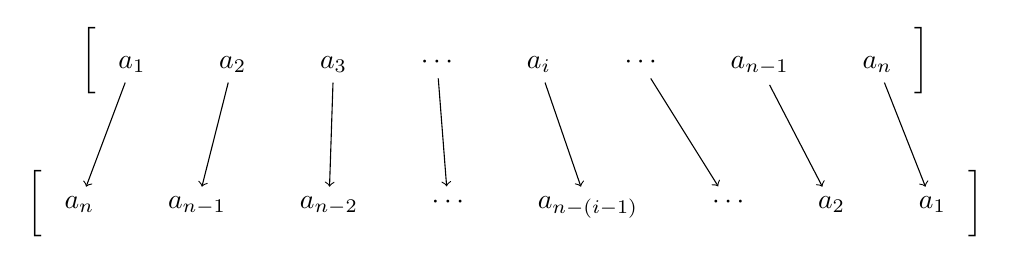
\begin{tikzpicture}[baseline=(current bounding box.center)]
  % Matrix A
  \matrix (A) [matrix of math nodes, left delimiter={[}, right delimiter={]}, row sep=1em, column sep=2em] {
    a_1 & a_2 & a_3 & \cdots & a_i & \cdots & a_{n-1} & a_n \\
  };

  % Matrix B
  \matrix (B) [matrix of math nodes, left delimiter={[}, right delimiter={]}, row sep=1em, column sep=2em, below=3em of A] {
    a_n & a_{n-1} & a_{n-2} & \cdots & a_{n-(i-1)} & \cdots & a_2 & a_1 \\
  };

  % Draw arrows from A_i to B_i
  \foreach \i in {1,2,3,4,5}
    \draw[->] (A-1-\i) -- (B-1-\i);

  % Optional: arrows for ellipsis and final element
  \draw[->] (A-1-6) -- (B-1-6); % for \cdots
  \draw[->] (A-1-7) -- (B-1-7); % for a_{n-1} → b_{n-1}
  \draw[->] (A-1-8) -- (B-1-8); % for a_n → b_n
\end{tikzpicture}
\]

\end{proof}

\end{theo}


\vspace{2em}


And since we are dealing with sequence transformations in this work, we might as well define the necessary transformer:

\vspace{1em}

\begin{transf}[The \textbf{Complement Transformer}\index{transformer!complement}]
\label{TRANSCOMPL}
$ $\\
$\Theta \xrightarrow{O_{complement}(\Theta)} \Theta^*; \quad \Theta^* = \lnot\Theta$\\
\end{transf}

\vspace{1em}


\section{Significance of Sequence Complements, $\lnot\Theta$, and Complement Symbol Sets, $\lnot\psi_\beta$}
\label{SECSIGCOMPLE}

First, we shall momentarily return to binary sequences. 

We note that, for some binary sequence $\Theta: \mathbb{N} \times \psi_{01}$, the transform

\vspace{1em}
\begin{trans}
$\Theta \xrightarrow{O_{complement}(\cdot)} \Theta^*; \Theta^* = \lnot\Theta$
\end{trans}
\vspace{1em}

which applies \textbf{\hyperref[TRANSCOMPL]{Transformer \ref{TRANSCOMPL}}}, produces a sequence of the same length as $\Theta$ but with all bits swapped/replaced by their complements, which, as per usual nomenclature in computer science for example, means the resultant sequence is produced from the source via a \textbf{bitwise NOT operation}, and which, for binary sequences, is as simple as merely flipping the bits individually.

Thus, if our source sequence was 

\vspace{1em}

\begin{equation}
\Theta = \langle 0 1 0 1 1 1 1 0 \rangle
\end{equation}

\vspace{1em}

Then 

\vspace{1em}

\begin{trans}
$\Theta \xrightarrow{O_{complement}(\Theta)}  \langle 1 0 1 0 0 0 0 1 \rangle$
\end{trans}

\vspace{1em}

And then, returning to nucleic acid sequences, we note that if we for example have some na-Sequence such as 

\vspace{1em}
\begin{equation}
\label{SEQATC}
\Theta = \langle A T C G C G T A T \rangle
\end{equation}

\vspace{1em}

\textbf{That we wish to treat as a DNA-sequence}, then its \textit{na-Complement}\index{na-Complement}\index{DNA!complement} sequence would be derivable from $\psi_{DNA}$ as such:

Since $\psi_{DNA} = \langle A, C, G, T \rangle$, then by \textbf{\hyperref[EQCOMPSETS]{Equation \ref{EQCOMPSETS}}}, we know that:

\vspace{1em}
\begin{equation}
\lnot(\psi_{DNA}) = \lnot\psi_{DNA}) = \langle T, G, C, A \rangle
\end{equation}
\vspace{1em}

So that, $\forall \rho \in \psi_{DNA}$, the equivalent complement is via the mapping:

\vspace{2em}

\[
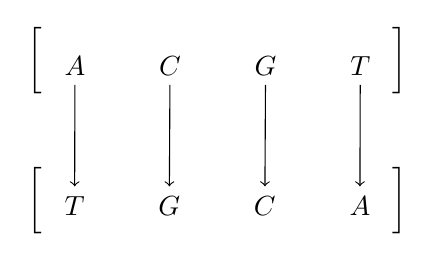
\begin{tikzpicture}[baseline=(current bounding box.center)]
  % Matrix A
  \matrix (A) [matrix of math nodes, left delimiter={[}, right delimiter={]}, row sep=1em, column sep=2em] {
    A & C & G & T \\
  };

  % Matrix B
  \matrix (B) [matrix of math nodes, left delimiter={[}, right delimiter={]}, row sep=1em, column sep=2em, below=3em of A] {
    T & G & C & A \\
  };

  % Draw arrows from A_i to B_i
  \foreach \i in {1,2,3, 4}
    \draw[->] (A-1-\i) -- (B-1-\i);
\end{tikzpicture}
\]

\vspace{2em}

Which is also the consequence of \textbf{\hyperref[THEOCOMPLEMENTS]{Theorem \ref{THEOCOMPLEMENTS}}}. Thus, for the sequence in \textbf{\hyperref[SEQATC]{Equation \ref{SEQATC}}}, the corresponding complement DNA sequence is:

\vspace{1em}
\begin{equation}
\label{SEQATCCOMP}
\lnot\Theta = \langle T A G C G C A T A \rangle
\end{equation}
\vspace{1em}

This ideal can be further appreciated by noticing that the traditional DNA sequence base symbol set (which we shall denote by $\dot{\psi}_{DNA}$\index{$\dot{\psi}_{DNA}$}), is actually different from $\psi_{DNA}$, and is defined as:

\vspace{1em}
\begin{equation}
\label{SSDNAT}
\dot{\psi}_{DNA} = \langle A, T, C, G \rangle
\end{equation}
\vspace{1em}

We should come to appreciate this special symbol set, or even justify it --- for logical and mathematical analyses, by acknowledging that it depicts not just a sequence of distinct symbols from $\psi_{DNA}$, but also their natural order based on both order of occurrence in $\psi_{DNA}$ \textbf{and} their equivalent \textbf{symbol complements} in $\lnot\psi_{DNA}$! It is such a terrific discovery/realization. And before we proceed, we note that the $\dot{\psi}_{DNA} \rightarrow \lnot\dot{\psi}_{DNA}$ mapping for pairwise-ordered DNA sequences is as such:

\vspace{2em}

\[
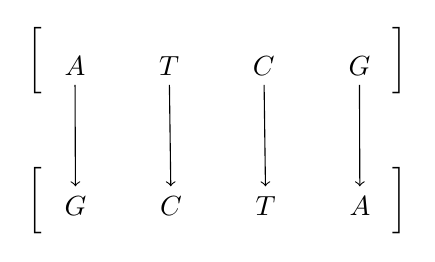
\begin{tikzpicture}[baseline=(current bounding box.center)]
  % Matrix A
  \matrix (A) [matrix of math nodes, left delimiter={[}, right delimiter={]}, row sep=1em, column sep=2em] {
    A & T & C & G \\
  };

  % Matrix B
  \matrix (B) [matrix of math nodes, left delimiter={[}, right delimiter={]}, row sep=1em, column sep=2em, below=3em of A] {
    G & C & T & A \\
  };

  % Draw arrows from A_i to B_i
  \foreach \i in {1,2,3, 4}
    \draw[->] (A-1-\i) -- (B-1-\i);
\end{tikzpicture}
\]

\vspace{2em}

Because, from \textbf{\hyperref[SSDNAT]{Equation \ref{SSDNAT}}}, we can tell that:

\vspace{1em}
\begin{equation}
\label{SSDNATCOMP}
\lnot\dot{\psi}_{DNA} = \langle G, C, T, A \rangle
\end{equation}
\vspace{1em}

Perhaps, and worth checking out, even if momentarily, what would happen when the idea of complement symbols sets and complement sequences is applied to the more commonplace base-10 sequences\index{sequences!decimal} (aka ``usual numbers"\footnote{And this shall not be a waste of space and time, since, as we shall find out in \textbf{\hyperref[SEC4]{Chapter \ref{SEC4}}}, base-10 symbols could underlie a very straight-forward system for implementing or theoretically exploring genome expression, a very important topic in all genetics!})?

First, note that since $\psi_{10}$ --- our choice of symbol for the decimal symbol set, is expressed as such:

\vspace{1em}
\begin{equation}
\label{SSDEC}
\psi_{10}= \langle 0, 1, 2, 3, 4, 5, 6, 7, 8, 9 \rangle
\end{equation}
\vspace{1em}

Then, by \textbf{\hyperref[THEOCOMPLEMENTS]{Theorem \ref{THEOCOMPLEMENTS}}}, its complement is:

\vspace{1em}
\begin{equation}
\label{SSDEC}
\lnot\psi_{10}= \langle 9, 8, 7, 6, 5, 4, 3, 2, 1, 0 \rangle
\end{equation}
\vspace{1em}

So that, for any base-10 digit, the corresponding \textbf{complement digit}\index{complement digit} is as in the mapping below:


\[
\begin{tikzpicture}[baseline=(current bounding box.center)]
  % Matrix A
  \matrix (A) [matrix of math nodes, left delimiter={[}, right delimiter={]}, row sep=1em, column sep=2em] {
    0 & 1 & 2 & 3 & 4 & 5 & 6 & 7 & 8 & 9\\
  };

  % Matrix B
  \matrix (B) [matrix of math nodes, left delimiter={[}, right delimiter={]}, row sep=1em, column sep=2em, below=3em of A] {
    9 & 8 & 7 & 6 & 5 & 4 & 3 & 2 & 1 & 0\\
  };

  % Draw arrows from A_i to B_i
  \foreach \i in {1,2,3,4,5,6,7,8,9,10}
    \draw[->] (A-1-\i) -- (B-1-\i);
\end{tikzpicture}
\]

Such a peculiar cipher! Because, usual/familiar number sequences such as the \textbf{Hi-Fi o-SSI}\cite{adtpaper}\index{Hi-Fi o-SSI}, defined as such:

\vspace{1em}
\begin{equation}
\Theta_{HiFi} = 8 6 4 9 1 3 7 5 2 0
\end{equation}
\vspace{1em}

Has the complement:

\vspace{1em}
\begin{equation}
\lnot\Theta_{HiFi} = 1 3 5 0 8 6 2 4 7 9
\end{equation}
\vspace{1em}

Which, given how that special sequence was derived/discovered(see \textbf{Section 5.1} in \cite{ossipaper} or \textbf{Equation 19} in the same paper), it is interesting to note that its complement under $\psi_{10}$ is also an \textit{orthogonal symbol set identity}\index{orthogonal symbol set identity}! For those who have studied the o-SSI paper\cite{ossipaper}, this can really be exciting for the study of symbol sets and sequences in general --- yes, even for nucleic acid sequences! But, that said, of course, it shouldn't come as a surprise, since, in simple terms, a sequence's complement is just one very special kind of anagram\index{anagram}\index{sequence!anagram} among the set of all potential anagrams it can have, and so, before we leave the base-10 case, we can note that if some sequence $\Theta_{10}: \mathbb{N} \times \psi_{10}$ is a base-10 o-SSI, then its complement is also a base-10 o-SSI, and in fact, in general --- even for non-numeric symbol sets such as $\psi_{na}, \psi_{DNA}$ or special $\psi_{RNA}$, that:

\vspace{2em}

\begin{theo}[\textbf{Complement of an o-SSI is an o-SSI}]
\label{THEOCOMPLOSSI}
If some sequence $\Theta: \mathbb{N} \times \psi_\beta$ is an orthogonal symbol set identity\index{symbol set!orthogonal} for the base $\beta$, then its complement, $\lnot\Theta$ is also an orthogonal symbol set identity for $\beta$.\\
\end{theo}

\vspace{2em}

We shall see how \textbf{\hyperref[THEOCOMPLOSSI]{Theorem  \ref{THEOCOMPLOSSI}}} might be applied, when dealing with algorithmic anagrammatization of sequences such as $\psi_{10}$ in \textbf{\hyperref[SECRSG]{Chapter \ref{SECRSG}}}.


\section{Potential Applications of Sequence Complements or Inverses}
\label{SECAPPCOMPLEMENTS}


First, in genetics and analysis of genetic code sequences, note that, for especially na-Sequences in say the \textit{non-native}(non-storage) form, such as the processed/derivative RNA-sequences, it might sometimes be useful to determine if some two sequences are the same, equivalent or closely related, even though their apparent ordering of members, or even member composition looks unlike, \textbf{as long as their cardinalities are the same}\footnote{This requirement to have their sizes the same, is a natural consequence of how a sequence and its anagrams relate --- see \cite{adtpaper}. However, once the basic concepts are well understood, this condition may be relaxed or merely be worked around. Also, for cases where we are concerned with sequence analysis and comparison where lengths either don't matter or are potentially different, refer to the kinds of analyses we conduct in the next chapter --- see \textbf{\hyperref[SEC4ASEQ]{Section \ref{SEC4ASEQ}}} for example.}.

We should note, and interestingly so, that the complement of any sequence $\Theta$, which is $\lnot\Theta$, is just an anagram of $\Theta$, and that in general, we can comfortably say:

\vspace{2em}


\begin{theo}[\textbf{Equivalence of Sequences under the Complement Transform\index{complement transform}}]
\label{THEOCOMPEQUIV}
If two sequences $\Theta$ and $\Omega$ that are \textbf{not equal}, do have the same cardinality and similar distribution of members, then they are essentially equivalent under the sequence complement transform and some projections of their form.

\begin{proof}
The proofs are several:
\begin{enumerate}
\item Since $\invpi(\Theta) = \invpi(\Omega)$ and $\forall \alpha \in \Theta \quad \exists \rho \in \Omega: \alpha = \rho$ or equivalently, that $\forall a_i \in \Theta, \invpi(a_i \in \Theta) = \invpi(a_i \in \Omega)$, then there exists some anagram of $\Theta$, denoted $\Theta^*$ such that $\Theta^* \xrightarrow{O_{complement}(\cdot)} \Omega$, which is possible by \textbf{\hyperref[THEOCOMPLEMENTS]{Theorem \ref{THEOCOMPLEMENTS}}}.
\item Because sequence complements are anagrams of each other, then if the two sequences are complements of each other, we expect that by the definition of the complement transformer (see \textbf{\hyperref[TRANSCOMPL]{Transformer \ref{TRANSCOMPL}}}), $\Omega = \lnot\Theta$ or that $\Theta = \lnot\Omega$.
\item We might also proceed by use of \textbf{modal sequences} (see \textbf{Definition 1} in \cite{transformatics}): Given the conditions on the two sequences, we then expect that if $\Theta$ is a sequence complement of $\Omega$ or vice-versa, then, computing their corresponding modal sequence statistic should result in the following result: $\overset{>}{\Theta} = \lnot(\overset{>}{\lnot\Omega})$ or equivalently, $\overset{>}{\Omega} = \lnot(\overset{>}{\lnot\Theta})$
\end{enumerate}
\end{proof}

\end{theo}

\vspace{2em}

Note that, for RNA, since $\psi_{RNA} = \langle A, C, G, U \rangle$ (\textbf{\hyperref[EQRNASS]{Equation \ref{EQRNASS}}}), then: 

\vspace{1em}

\begin{equation}
\label{EQRNACOMP}
\lnot\psi_{RNA} = \langle U, G, C, A \rangle
\end{equation}

\vspace{1em}

And this is what we'd expect via the complement mapping:

\vspace{1em}

\[
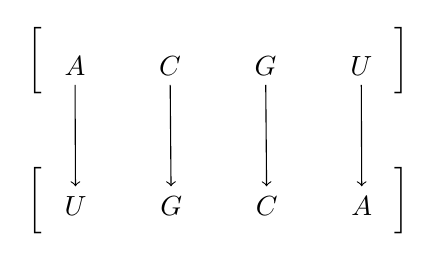
\begin{tikzpicture}[baseline=(current bounding box.center)]
  % Matrix A
  \matrix (A) [matrix of math nodes, left delimiter={[}, right delimiter={]}, row sep=1em, column sep=2em] {
    A & C & G & U \\
  };

  % Matrix B
  \matrix (B) [matrix of math nodes, left delimiter={[}, right delimiter={]}, row sep=1em, column sep=2em, below=3em of A] {
    U & G & C & A \\
  };

  % Draw arrows from A_i to B_i
  \foreach \i in {1,2,3, 4}
    \draw[->] (A-1-\i) -- (B-1-\i);
\end{tikzpicture}
\]

\vspace{1em}

But, since the traditional pairwise ordered symbol set for RNA, $\dot{\psi}_{RNA}$ is

\vspace{1em}

\begin{equation}
\label{EQRNATRAD}
\dot{\psi}_{RNA} = \langle A, U, C, G \rangle
\end{equation}

\vspace{1em}

Then its corresponding complement,$\lnot\dot{\psi}_{RNA}$, is

\vspace{1em}

\begin{equation}
\label{EQRNATRADCOMP}
\lnot\dot{\psi}_{RNA} = \langle G, C, U, A \rangle
\end{equation}

\vspace{1em}

And so we have the associated complement mapping as

\vspace{1em}


\[
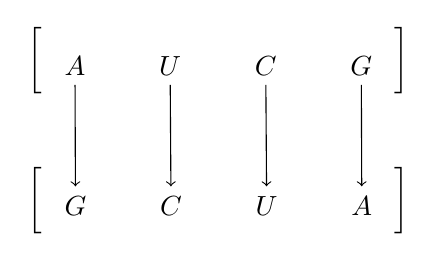
\begin{tikzpicture}[baseline=(current bounding box.center)]
  % Matrix A
  \matrix (A) [matrix of math nodes, left delimiter={[}, right delimiter={]}, row sep=1em, column sep=2em] {
    A & U & C & G \\
  };

  % Matrix B
  \matrix (B) [matrix of math nodes, left delimiter={[}, right delimiter={]}, row sep=1em, column sep=2em, below=3em of A] {
    G & C & U & A \\
  };

  % Draw arrows from A_i to B_i
  \foreach \i in {1,2,3, 4}
    \draw[->] (A-1-\i) -- (B-1-\i);
\end{tikzpicture}
\]

\vspace{1em}

So, that, for some RNA-sequence such as $\Theta_{met}$:

\vspace{1em}

\begin{equation}
\Theta_{met} = \langle A, U, G \rangle
\end{equation}

\vspace{1em}

Which is the famous START-codon \textbf{Methionine} (see \textbf{\hyperref[TAB2]{Table \ref{TAB2}}}), has as its corresponding nucleic acid sequence complement under $\dot{\psi}_{RNA}$:

\vspace{1em}

\begin{trans}
\label{TRANSGCA}
$\Theta_{met} \xrightarrow{O_{complement}(\Theta,\dot{\psi}_{RNA})}  \langle G, C, A \rangle$\\
That codon\index{codon} isn't the same as the source (ATG/AUG/Methionine), but there's some debate concerning what it actually is called --- \textbf{Table 1} in \cite{gregory1987oxford} names codon GCA as \textbf{Arginine}, while Wikipedia\cite{wikipedia_codon_tables} names it \textbf{Alanine}.
\end{trans}

\vspace{1em}

While --- \textbf{and important to note}, its complement under $\psi_{RNA}$ is [indeed] different!

\vspace{1em}

\begin{trans}
\label{TRANSUAC}
$\Theta_{met} \xrightarrow{O_{complement}(\Theta,\psi_{RNA})}  \langle U, A, C \rangle$
\\
and we know that codon UAC is Tyrosine\cite{wikipedia_codon_tables}\footnote{Concerning this particular codon, TAC/UAC, we find that though the Wikipedia reference tables assign it the name Tyrosine in both the DNA and RNA encodings, and yet, the physical reference we have at hand\cite{gregory1987oxford} (perhaps now out-of-date), assigns the name ``Methionine" to TAC --- Table 1 in that reference book did not list RNA codes, but we still would expect to use TAC to look-up the correct name for UAC.}.
\end{trans}

\vspace{1em}

It should perhaps be immediately noticeable that the ability to derive new/different/special sequences such as complement codons\index{codon!complements}\index{complement codon} from ordinary na-Sequences might have some useful if not exciting applications as well as problems it awakens for the geneticists, molecular biologists and researchers of gene-sequencing\footnote{For those that do not know: Gene sequencing is the process of determining the exact order of nucleotides --- A, T, C and G --- in a segment of DNA that makes up a gene. It is like reading the biological ``code" that instructs cells how to build proteins and regulate functions\cite{copilot_dna_assistant}.} and analysis. For example, apart from acknowledging that na-Sequence's complements denote potentially legitimate na-helix strand partners for any two sequences (in the form $\Theta$ and $\lnot\Theta$), it would be further rewarding, to determine what other important things we might learn about how important sequences such as na-Sequences --- especially relative to how they are utilized in nature, behave or alter their usual function, if replaced by their complements either partially or wholly. Definitely, true for any sequences in general... it must be exhilarating to discover what other things we can learn with or from them, via these kinds of sequence transforms. 




\begin{center}
\fbox{\begin{minipage}{0.9\textwidth}
\LARGE
More \textbf{FUTURE WORK} for GENETICS Researchers:\\

It is already interesting to note that, under complement transforms\index{complement transform} (which are special kinds of anagrams), the natural/universal protein synthesis START-codon AUG/ATG is equivalent to GCA (\textbf{\hyperref[TRANSGCA]{Transformation \ref{TRANSGCA}}}) or UAC (\textbf{\hyperref[TRANSUAC]{Transformation \ref{TRANSUAC}}}), but, \textbf{are those other codons also START-codons?} That said, is there a possibility that some natural process or genetic code translation or transformation might naturally produce ATG or AUG from any of those corresponding [symbolic] complement sequences? What would this teach us about natural/biological processors? What of the possibilities of using synthetic/artificial processors to render such complement operations useful? And is it actually possible to \textit{transmute} one set of nucleic acid sequences into another, with entirely different functions and identity via leveraging na-complements or complement transforms\index{complement transform}?


\end{minipage}}
\\
\end{center}



\chapter{Sequence Analysis Using The Anagram Distance and the Modal Sequence Statistic}
\label{SEC4A}



We are going to talk about the matter of comparing or analyzing two or more na-Sequences using especially statistical measures that have been set down by transformatics theory for especially sequences of the kind we are interested in when exploring work in genetics. 

\section{Six Sequences and Four Scenarios}
\label{SEC4ASEQ}

In particular, we shall be looking at na-Sequence analysis\index{sequence analysis} through lens of measures we have formalized earlier on\footnote{For those not yet familiar with the existing mathematical theories and results of transformatics, \textbf{\hyperref[CHAPTRANS]{Chapter \ref{CHAPTRANS}}} in the appendix does provide all the necessary background context relevant for mastering all the new [applied transformatics] material we are exploring in this chapter.}, and shall break down our analysis into four representative scenarios:

\begin{enumerate}
\item \textbf{Scenario A:} Given some two particular instances of na-Sequences, $\Theta1_n$ and $\Theta2_n$, \textbf{not necessarily the same} ($(\Theta1_n = \Theta2_n) \quad \lor \quad (\Theta1_n \neq \Theta2_n)$), but which are of the same length, $\invpi(\Theta1_n) = \invpi(\Theta2_n) = n$, and with similar symbol sets\footnote{\textbf{NOTE} that in this case we are expressing this problem aspect using specific symbol sets --- such as $\hat{\psi}_{na}(\Theta1_n)$ --- and not say unspecific symbol sets ($\hat{\psi}(\Theta1_n)$), nor implicit symbol sets ($\psi(\Theta1_n)$), and neither natural symbol sets ($\psi_{na}(\Theta1_n)$), because, we do not wish to assume that the two sequences have the same exact ordering of distinct elements from the specified base symbol set --- $\psi_{na}$ --- a fact which for example the natural symbol set can't show/preserve, and yet, because we know the base, we do not want to only deal with base-less symbol sets such would be the case with the unspecific and implicit symbol set. For details concerning these different symbol sets, refer to the clarifying discussion offered in \textbf{Question 4} of \cite{transformatics_interview}.}, $(\hat{\psi}_{na}(\Theta1_n) \cong \hat{\psi}_{na}(\Theta2_n)) \quad \land \quad (\invpi(\psi_{na}(\Theta1_n)) = \invpi(\psi_{na}(\Theta2_n)) \leq n)$, \textbf{how to quantify how similar or dissimilar} they are?
\item \textbf{Scenario B:} Given some two particular instances of na-Sequences, $\Theta1_n$ and $\Theta2_k$, still not necessary the same, and of different lengths, $(\invpi(\Theta1_n) = n) \neq (\invpi(\Theta2_k) = k)$, but with \textbf{similar symbol sets}, $(\hat{\psi}_{na}(\Theta1_n) \cong \hat{\psi}_{na}(\Theta2_k)) \quad \land \quad (\invpi(\psi_{na}(\Theta1_n)) = \invpi(\psi_{na}(\Theta2_k)) \leq Min(n,k))$, how to quantify how similar or dissimilar they are?
\item \textbf{Scenario C:} Given some two \textbf{potentially different}, particular instances of na-Sequences, $\Theta1_n$ and $\Theta2_k$, of \textbf{different lengths}, $n$ and $k$, and \textbf{with different symbol sets}, $((\hat{\psi}_{na}(\Theta1_n) \neq \hat{\psi}_{na}(\Theta2_k)) \quad \lor \quad (\invpi(\psi_{na}(\Theta1_n)) \neq \invpi(\psi_{na}(\Theta2_k))))$, how to quantify how similar or dissimilar they are?
\item \textbf{Scenario D:} Finally, how, when given a particular na-Sequence, $Q_k$, and two collections/samples of other sequences\\
 ($\Theta1, \Theta2, \Theta3,..., \Theta m$) and ($\Omega1, \Omega2, \Omega3,..., \Omega n$) of potentially dissimilar lengths, $m$ and $n$ respectively, and that belong to \textbf{labeled or classified populations} --- POPA and POPB respectively, to determine which of the two populations the query sequence, $Q_k$, best-belongs to (so we classify it under the associated label), as well as determine which of the \textbf{particular} sample's member sequences --- from that chosen collection it is closest to.
\end{enumerate}

Note that, in conducting these analyses, we shall especially exploit the sequence-specific measures, $\tilde{A}(\cdot)$, the Anagram Distance Measure\cite{adtpaper}\cite{transformatics}, and $\overset{>}{\Theta}$, the Modal Sequence Statistic\cite{transformatics}, and that we shall use the following representative, even though somewhat hypothetical (for the first four), na-Sequences\index{na-Sequence}\index{genetic sequence}\index{DNA!examples}:

\begin{equation}
{\Theta1}_{DNA} = \langle TAC GGG CAT TCC \rangle\\
\end{equation}

\begin{equation}
{\Theta2}_{RNA} = \langle AUG AUG CGC GGG CAT AUC \rangle\\
\end{equation}

\begin{equation}
{\Theta3}_{DNA} = \langle ATA ATGG GGG CAT TGA \rangle\\
\end{equation}

\begin{equation}
{\Theta4}_{DNA} = \langle TAC TCC GGG CAT\rangle\\
\end{equation}

\begin{multline}
\Theta_{insulin} =  \texttt{ATGGCCCTGTGGATGCGCCTCCTGCCCCTGCTGGCGCTGCTGGCCCTCTGGGGACC}\\
\texttt{CCAGCCGCAGCCTTTGTGAACCAACACCTGTGCGGCTCACACCTGGTGGAAGCTCTCTAC}\\
\texttt{CTAGTGTGCGGGGAACGAGGCTTCTTCTACACACCCAAGACCCGCCGGGAGGCAGAGGAC}\\
\texttt{CTGCAGGTGGGGCAGGTGGAGCTGGGCGGGGGCCCTGGTGCAGGCAGCCTGCAGCCCTTG}\\
\texttt{GCCCTGGAGGGGTCCCTGCAGAAGCGTGGCATTGTGGAACAATGCTGTACCAGCATCTGC}\\
\texttt{TCCCTCTACCAGCTGGAGAACTACTGCAACTAG}
\end{multline}

\small
\begin{multline}
\Theta_{rbcl} = 
AUGAAUUGCUUUGGAGGAGUUGCUUUGGCUUUGGAGGAGUUUGCUUUGGCUUUGGAGGAG\\
UUUGCUUUGGCUUUGGAGGAGUUUGCUUUGGCUUUGGAGGAGUUUGCUUUGGCUUUGGAG\\
GAGUUUGCUUUGGCUUUGGAGGAGUUUGCUUUGGCUUUGGAGGAGUUUGCUUUGGCUUUG\\
GAGGAGUUUGCUUUGGCUUUGGAGGAGUUUGCUUUGGCUUUGGAGGAGUUUGCUUUGGCU\\
UUGGAGGAGUUUGCUUUGGCUUUGGAGGAGUUUGCUUUGGCUUUGGAGGAGUUUGCUUUG\\
GCUUUGGAGGAGUUUGCUUUGGCUUUGGAGGAGUUUGCUUUGGCUUUGGAGGAGUUUGCU\\
UUGGCUUUGGAGGAGUUUGCUUUGGCUUUGGAGGAGUUUGCUUUGGCUUUGGAGGAGUUU\\
GCUUUGGCUUUGGAGGAGUUUGCUUUGGCUUUGGAGGAGUUUGCUUUGGCUUUGGAGGAG\\
UUUGCUUUGGCUUUGGAGGAGUUUGCUUUGGCUUUGGAGGAGUUUGCUUUGGCUUUGGAG\\
GAGUUUGCUUUGGCUUUGGAGGAGUUUGCUUUGGCUUUGGAGGAGUUUGCUUUGGCUUUG\\
GAGGAGUUUGCUUUGGCUUUGGAGGAGUUUGCUUUGGCUUUGGAGGAGUUUGCUUUGGCU\\
UUGGAGGAGUUUGCUUUGGCUUUGGAGGAGUUUGCUUUGGCUUUGGAGGAGUUUGCUUUG\\
GCUUUGGAGGAGUUUGCUUUGGCUUUGGAGGAGUUUGCUUUGGCUUUGGAGGAGUUUGCU\\
UUGGCUUUGGAGGAGUUUGCUUUGGCUUUGGAGGAGUUUGCUUUGGCUUUGGAGGAGUUU\\
GCUUUGGCUUUGGAGGAGUUUGCUUUGGCUUUGGAGGAGUUUGCUUUGGCUUUGGAGGAG\\
UUUGCUUUGGCUUUGGAGGAGUUUGCUUUGGCUUUGGAGGAGUUUGCUUUGGCUUUGGAG\\
GAGUUUGCUUUGGCUUUGGAGGAGUUUGCUUUGGCUUUGGAGGAGUUUGCUUUGGCUUUG\\
GAGGAGUUUGCUUUGGCUUUGGAGGAGUUUGCUUUGGCUUUGGAGGAGUUUGCUUUGGCU\\
UUGGAGGAGUUUGCUUUGGCUUUGGAGGAGUUUGCUUUGGCUUUGGAGGAGUUUGCUUUG\\
GCUUUGGAGGAGUUUGCUUUGGCUUUGGAGGAGUUUGCUUUGGCUUUGGAGGAGUUUGCU\\
UUGGCUUUGGAGGAGUUUGCUUUGGCUUUGGAGGAGUUUGCUUUGGCUUUGGAGGAGUUU\\
GCUUUGGCUUUGGAGGAGUUUGCUUUGGCUUUGGAGGAGUUUGCUUUGGCUUUGGAGGAG\\
UUUGCUUUGGCUUUGGAGGAGUUUGCUUUGGCUUUGGAGGAGUUUGCUUUGGCUUUGGAG\\
GAGUUUGCUUUGGCUUUGGAGGAGUUUGCUUUGGCUUUGGAGGAGUUUGCUUUGGCUUUG\\
GAGGAGUUUGCUUUGGCUUUGGAGGAGUUUGCUUUGGCUUUGGAGGAGUUUGCUUUGGCU\\
UUGGAGGAGUUUGCUUUGGCUUUGGAGGAGUUUGCUUUGGCUUUGGAGGAGUUUGCUUUG\\
GCUUUGGAGGAGUUUGCUUUGGCUUUGGAGGAGUUUGCUUUGGCUUUGGAGGAGUUUGCU\\
UUGGCUUUGGAGGAGUUUGCUUUGGCUUUGGAGGAGUUUGCUUUGGCUUUGGAGGAGUUU\\
GCUUUGGCUUUGGAGGAGUUUGCUUUGGCUUUGGAGGAGUUUGCUUUGGCUUUGGAGGAG\\
UUUGCUUUGGCUUUGGAGGAGUUUGCUUUGGCUUUGGAGGAGUUUGCUUUGGCUUUGGAG\\
GAGUUUGCUUUGGCUUUGGAGGAGUUUGCUUUGGCUUUGGAGGAGUUUGCUUUGGCUUUG\\
GAGGAGUUUGCUUUGGCUUUGGAGGAGUUUGCUUUGGCUUUGGAGGAGUUUGCUUUGGCU\\
UUGGAGGAGUUUGCUUUGGCUUUGGAGGAGUUUGCUUUGGCUUUGGAGGAGUUUGCUUUG\\
GCUUUGGAGGAGUUUGCUUUGGCUUUGGAGGAGUUUGCUUUGGCUUUGGAGGAGUUUGCU\\
UUGGCUUUGGAGGAGUUUGCUUUGGCUUUGGAGGAGUUUGCUUUGGCUUUGGAGGAGUUU\\
GCUUUGGCUUUGGAGGAGUUUGCUUUGGCUUUGGAGGAGUUUGCUUUGGCUUUGGAGGAG\\
UUUGCUUUGGCUUUGGAGGAGUUUGCUUUGGCUUUGGAGGAGUUUGCUUUGGCUUUGGAG\\
GAGUUUGCUUUGGCUUUGGAGGAGUUUGCUUUGGCUUUGGAGGAGUUUGCUUUGGCUUUG\\
GAGGAGUUUGCUUUGGCUUUGGAGGAGUUUGCUUUGGCUUUGGAGGAGUUUGCUUUGGCU\\
UUGGAGGAGUUUGCUUUGGCUUUGGAGGAGUUUGCUUUGGCUUUGGAGGAGUUUGCUUUG\\
GCUUUGGAGGAGUUUGCUUUGGCUUUGGAGGAGUUUGCUUUGGCUUUGGAGGAGUUUGCU\\
UUGGCUUUGGAGGAGUUUGCUUUGGCUUUGGAGGAGUUUGCUUUGGCUUUGGAGGAGUUU\\
GCUUUGGCUUUGGAGGAGUUUGCUUUGGCUUUGGAGGAGUUUGCUUUGGCUUUGGAGGAG\\
UUUGCUUUGGCUUUGGAGGAGUUUGCUUUGGCUUUGGAGGAGUUUGCUUUGGCUUUGGAG\\
GAGUUUGCUUUGGCUUUGGAGGAGUUUGCUUUGGCUUUGGAGGAGUUUGCUUUGGCUUUG\\
GAGGAGUUUGCUUUGGCUUUGGAGGAGUUUGCUUUGGCUUUGGAGGAGUUUGCUUUGGCU\\
UUGGAGGAGUUUGCUUUGGCUUUGGAGGAGUUUGCUUUGGCUUUGGAGGAGUUUGCUUUG\\
GCUUUGGAGGAGUUUGCUUUGGCUUUGGAGGAGUUUGCUUUGGCUUUGGAGGAGUUUGCU\\
UUGGCUUUGGAGGAGUUUGCUUUGGCUUUGGAGGAGUUUGCUUUGGCUUUGGAGGAGUUU\\
GCUUUGGCUUUGGAGGAGUUUGCUUUGGCUUUGGAGGAGUUUGCUUUGGCUUUGGAGGAG\\
UUUGCUUUGGCUUUGGAGGAGUUUGCUUUGGCUUUGGAGGAGUUUGCUUUGGCUUUGGAG\\
GAGUUUGCUUUGGCUUUGGAGGAGUUUGCUUUGGCUUUGGAGGAGUUUGCUUUGGCUUUG\\
GAGGAGUUUGCUUUGGCUUUGGAGGAGUUUGCUUUGGCUUUGGAGGAG
\end{multline}
\Large


The first four sequences are merely hypothetical, and intentionally small/short, with $\Theta1_{DNA}$, $\Theta3_{DNA}$ and $\Theta4_{DNA}$ being DNA-sequences, while $\Theta2_{RNA}$ is just some RNA-sequence. $\Theta_{insulin}$ is a DNA-sequence we have already encountered in \textbf{\hyperref[SEC2]{Chapter \ref{SEC2}}} (see \textbf{\hyperref[EQINSULIN]{Equation \ref{EQINSULIN}}}), while the most verbose sequence we shall encountered in this work is named $\Theta_{rbcl}$ and is a real-life, biologically relevant RNA-sequence from a well-known plant protein: \textbf{RbcL}\footnote{$\Theta_{rbcl}$ is actually just a sample mRNA Sequence (partial, from \textit{Arabidopsis thaliana} RbcL gene), and is excerpted from a paper that includes the \textit{Arabidopsis thaliana} chloroplast genome, which contains the rbcL gene encoding the large subunit of RuBisCO\cite{Sato1999ArabidopsisChloroplastGenome}.}, the large subunit of \textbf{RuBisCO} --- the enzyme responsible for carbon fixation in photosynthesis. It is one of the most abundant and essential proteins in plants\cite{copilot_dna_assistant}.

\section{A First Analysis}
\label{SECFANAL}


%draw horizontal line
\noindent\rule{\textwidth}{0.4pt}
{


\noindent\textbf{NOTE:}\\
\noindent\textbf{TEA programming language INSTALLATION and Basic USAGE Instructions}

\normalsize
\vspace{2em}

TEA as a language\index{TEA!installation guide} is designed to be usable from almost anywhere there is a computer capable of running the TEA language interpreter --- currently implemented for WEB (browser environments) using JavaScript, and for all other environments via Python3. However, to really get started using TEA, especially when one has a modern computer, a smartphone or some device capable of accessing the Internet and rendering web pages, one then need not install anything or download anything apart from merely visiting the following link:

\vspace{1em}
\textbf{TEA WEB IDE:} \url{https://tea.nuchwezi.com}
\vspace{1em}

So that, by visiting that page, one can readily access a usable basic and standard interface with which they can not only write, browse, read and run existing TEA programs --- especially those sample/example applications that are made available as part of the growing list of ``Standard TEA programs" --- but that they can also share the TEA program source code either using links, or copy-pasted codes. Using the WEB IDE is the simplest, best method for trying out TEA that is also beginner-friendly. Also, other than accessing the TEA programs and runtime, the IDE offers access to a TEA debugger for help with analyzing or troubleshooting problematic TEA programs, access to the TEA documentation, links to the TEA community, lecture notes and videos, etc.

For those that need to use TEA from any other environment or platform other than the web --- such as in non-interactive server-side programs, in command-line scripts, in stand-alone desktop programs, etc. The following installation method is what is currently most recommended:

\begin{enumerate}
\item To INSTALL TTTT and the TEA language [\textit{plus some standard TEA programs packaged together with TTTT; ZHA and AMC}\footnote{Users of TEA via the WEB IDE automatically get access to all (30+) standard TEA programs/example applications, however, for users of TEA via the Debian package tttt, only a few of these applications are currently included/accessible via the default installation method --- \textbf{ZHA}; the ``Zee Hacker Assistant" and \textbf{AMC}; Advanced Mathematics Computer}.] on your system, run the following command in your terminal:

    \begin{tcbverbatim}[title=UNIX/Linux TEA installation command]
curl -Ls https://bit.ly/installtea | bash
  \end{tcbverbatim}
\end{enumerate}

Once TEA is installed via the above command-line method, one can then readily view/browse the official documentation that comes along with that package via: \texttt{man tttt}

}

%draw horizontal line
\noindent\rule{\textwidth}{0.4pt}
\vspace{2em}



Before we dive into the matter of solving the analytic problems under the four scenarios introduced in \textbf{\hyperref[SEC4ASEQ]{Section \ref{SEC4ASEQ}}} above, we shall want to begin with a background analysis that shall give us some high-level insights about any of the sequences in our problem set. In particular, we are going to start by analyzing each of those sequences, so as to know the following basic facts:

\begin{enumerate}
\item What is the sequence's symbol set: $\psi(\Theta) = ?$
\item Which of the three nucleic acid symbol sets does the sequence belong to --- $\psi_{DNA}$, $\psi_{RNA}$ or $\psi_{na}$
\item What is the relative frequency of each sequence's symbol-set members? $\forall \rho \in \psi(\Theta), \invpi(\rho \in \Theta) = ?$
\item How long is the sequence as a flat-structure sequence: $\invpi(\Theta) = ?$
\item How many codons does the sequence contain? $\Theta \rightarrow \Theta^*: \mathbb{N} \times \psi_{na}^3, \invpi(\Theta^*) = ?$
\end{enumerate}

For purposes of helping others replicate the analyses and results we shall obtain, we recommend that the following analysis method be used: 


\textbf{We shall use TEA}\footnote{Instructions for how to install and use TEA/Transforming Executable Alphabet general-purpose text-processing oriented computer programming language are offered via the project's GitHub: \url{https://github.com/mcnemesis/cli_tttt} --- but also check the associated note presented at the start of this section | Otherwise, also note that one can readily try TEA as well as run any of the TEA programs we have included in this chapter and anywhere in the book, without installing any special software, merely by visiting the online, browser-based \textbf{TEA WEB IDE} via \url{https://tea.nuchwezi.com}}\cite{Lutalo2024_taz}\cite{cli_tttt} --- a text-processing-oriented general-purpose computer programming language --- an executable software language by the author, via its \texttt{tttt} Linux package and utility, to implement most of the analyses we wish to conduct via the command-line.

\begin{enumerate}
\item {\textbf{To Process a Sequence via the Command-Line?} For example, copy-and-paste sequence $\Theta1$ into a file named \texttt{theta1\_dna.txt}}
\item {\textbf{To compute the sequence symbol set?} For example, for $\Theta1$, run the following command against the sequence file to display the unique symbols in the sequence, in their natural order of first-occurrence within the sequence:

\vspace{1em}
\begin{verbatim}
cat theta1_dna.txt | tttt -c "b:"
TACG
\end{verbatim}
\vspace{1em}

}
\item {\textbf{To compute the modal sequence statistic?} First, note that the \textbf{modal sequence statistic} is well introduced, defined and how to use it demonstrated in \cite{transformatics}\footnote{See \textbf{Definition 1} in \cite{transformatics}, but also refer to \textbf{\hyperref[PROP5]{Proposal 5}} in \textbf{\hyperref[CHAPTRANS]{Chapter \ref{CHAPTRANS}}}.}. That said, for example, for $\Theta1$, run the following command against the sequence file to display the unique symbols in the sequence, in their order of most frequent first, but also their natural order of first-occurrence within the sequence:

\vspace{1em}
\begin{verbatim}
cat theta1_dna.txt | tttt -c "u!"":"
CTGA
\end{verbatim}
\vspace{1em}

Note that, the actual command/TEA-code for this is just \texttt{u!:}\index{TEA program!modal sequence statistic}, however, because of the way the Linux command-line treats the `!' symbol as a special character --- even inside strings, we must cleverly use it in a manner such as shown; we write ``u!"``:" to avoid the \textit{``unrecognized history modifier"} error if that code is written directly on the terminal. This shall apply to all the other cases where we must deal with the TEA command qualifier `!"\cite{Lutalo2024_taz}.

The other workaround is to \textbf{first turn off the BASH history expansion modifier} --- this, so that we can just write clean TEA code such as \texttt{u!:} without errors, directly on the Linux terminal interface. So, to disable history expasion for the \textit{active/current session} in your terminal, just run the command:

\vspace{1em}
\begin{verbatim}
set +H
\end{verbatim}
\vspace{1em}

And after that, you can just write clean TEA code for the above task as such:

\vspace{1em}
\begin{verbatim}
cat theta1_dna.txt | tttt -c u!:
CGTA
\end{verbatim}
\vspace{1em}
}
\item {\textbf{To compute the distribution of symbols within a sequence?} For example, to compute how many times the symbol `T' occurs in $\Theta1$, we can merely run the code:

\vspace{1em}
\begin{verbatim}
cat theta1_dna.txt | tttt -c "d!:T|g:|v:|v!:"
3
\end{verbatim}
\vspace{1em}

And for the symbol `C', we just modify that code to count for `C' as such:

\vspace{1em}
\begin{verbatim}
cat theta1_dna.txt | tttt -c "d!:C|g:|v:|v!:"
4
\end{verbatim}

\vspace{1em}

But if we wish to do the same for all distinct symbols within the sequence $\Theta1$ --- \textbf{and especially without having to explicitly list which symbols we are counting within the TEA code} --- meaning, no \textit{hard-coding} of the elements from the sequence's specific symbol set --- and equivalently, merely making the program symbol-set-independent --- or rather ``applicable to any sequence file", we could have used ``u!:" as in the previous task, since that TEA command counts how many times each unique symbol occurs in a sequence so as to compute the modal sequence, however, currently (with TEA version \textbf{1.3.6}\cite{cli_tttt}), the actual frequencies aren't returned with the output of ``u!:", and so, we shall want to use a work-around\footnote{\textbf{FUTURE WORK:} Provide a basic, in-built capability within the TEA instruction set, to allow for the automatic computation of a text sequence characteristic, $\hbar(\overset{>}{\Theta})$.} leveraging the above method for computing the frequency of each symbol in the input sequence. We can use the following non-trivial TEA program\index{program!Sequence Characteristic} for that then:

\vspace{1em}

    \begin{tcbverbatim}[title=EXAMPLE: Computing Sequence Characteristic\index{TEA program!sequence characteristic} using TEA on command line]
 cat theta1_dna.txt | tttt -c "v:vSEQ|v:vANA:{}|u!:|v:vMS|l:lMS|y:vMS|d!:^.|v:vSY|y:vMS|d:^.|v:vMS|y:vSEQ|d*!:vSY|g:|v:|v!:|v:vSYN|g*:{}:vSY:vSYN|x*:vANA|v:vANA|y:vMS|f:^$:lFIN|j:lMS|l:lFIN|y:vANA"
C4T3G3A2 
  \end{tcbverbatim}
  
  \vspace{1em}

The essential result from running that program against $\Theta1$ is the string \textbf{C4T3G3A2}, which tells us that `C' occurs 4 times, `T' 3 times, ... , and then `A' only 2 times --- the symbols in the sequence, and their frequencies, sorted in descending order of most frequent (mode) first, otherwise by their natural order of first occurrence (when two symbols have same frequency). 
}
\item {\textbf{To compute the cardinality of a sequence?} For example, for $\Theta2$, run the following command against the sequence file to display the total number of all symbols within the sequence:

\vspace{1em}

\begin{verbatim}
cat theta2_rna.txt | tttt -c "v:|v!:"
18
\end{verbatim}

\vspace{1em}

To confirm if TEA is telling us the correct thing, we can also count the characters in that sequence (assuming we pasted just the sequence symbols into the file and nothing else, and no delimiters between them), using the standard Linux/Unix command ``wc'' as such:

\vspace{1em}

\begin{verbatim}
cat theta2_rna.txt | wc -c
18
\end{verbatim}

}
\end{enumerate}


Such is the power of the sequence analysis we can do with the TEA language, without any sophisticated tools. Thus shall we analyze all the other sequences in our problem set, and to simplify things, we shall merely tabulate the analysis results for all six sequences as such:


\begin{table}[H]
  \Large
	\begin{tabular}[t]{|p{1.5cm}||p{3cm}|p{2cm}|p{6cm}|p{1.5cm}|p{1.5cm}|}
	\hline
	na-Seq & Unspecific Sequence Symbol Set: $\hat{\psi}(\Theta)$ & Closest Parent Symbol Set & \makecell{Modal Sequence\\Statistic, $\overset{>}{\Theta}$\\ and Symbol\\ Distribution:\\ $\invpi(\rho \in \Theta)$} & $\invpi(\Theta)$ &  \makecell{Codon\\ Count:\\ $\invpi(\Theta^*)$\\ $\approx \frac{\invpi(\Theta)}{3}$}\\
	\hline
	\hline
	
	%first sequence...
	${\Theta1}_{DNA}$ & $\langle T, A, C, G \rangle$ & $\psi_{DNA}$ &  
	\centering
	\begin{tabular}[t]{|c|c|c|c|}
		C & T & G & A\\
		\hline
		4 & 3 & 3 & 2\\	
		\hline
	 \end{tabular} & 12 & 4\\
		\hline	 
	\hline
	
	%second sequence...
	${\Theta2}_{RNA}$ & $\langle A, U, G, C, T \rangle$ & $\psi_{na}$ &  
	\centering
	\begin{tabular}[t]{|c|c|c|c|c|}
		G & A & C & U & T\\
		\hline
		6 & 4 & 4 & 3 & 1\\	
		\hline
	 \end{tabular} & 18 & 6\\
	 
		\hline	 
	\hline

%third sequence...
	${\Theta3}_{DNA}$ & $\langle A, T, G, C \rangle$ & $\psi_{DNA}$ &  
	\centering
	\begin{tabular}[t]{|c|c|c|c|}
		G & A & T & C\\
		\hline
		6 & 5 & 4 & 1\\	
		\hline
	 \end{tabular} & 16 & $5.3\bar{3}$\\
	\hline	 
	\hline
	
	
	%fourth sequence...
	${\Theta4}_{DNA}$ & $\langle T, A, C, G \rangle$ & $\psi_{DNA}$ &  
	\centering
	\begin{tabular}[t]{|c|c|c|c|}
		C & T & G & A\\
		\hline
		4 & 3 & 3 & 2\\	
		\hline
	 \end{tabular} & 12 & 4\\
	\hline	 
	\hline
	
	
	%fourth sequence...
	${\Theta}_{insulin}$ & $\langle A, T, G, C \rangle$ & $\psi_{DNA}$ &  
	\centering
	\begin{tabular}[t]{|c|c|c|c|}
		G & C & T & A\\
		\hline
		108 & 105 & 60 & 56\\	
		\hline
	 \end{tabular} & 329 & $109.6\bar{6}$\\
	\hline	 
	\hline
	
	%fifth sequence...
	${\Theta}_{rbcl}$ & $\langle A, U, G, C \rangle$ & $\psi_{RNA}$ &  
	\centering
	\begin{tabular}[t]{|c|c|c|c|}
		U & G & A & C\\
		\hline
		1355 & 1207 & 305 & 301\\	
		\hline
	 \end{tabular} & 3168 & 1056\\
	\hline	 
	\hline	
	
	              
\end{tabular}
 \caption{A First Analysis of the 5 na-Sequences from \textbf{\hyperref[SEC4ASEQ]{Section \ref{SEC4ASEQ}}}}
  \label{TABFAN}
\end{table}


\vspace{2em}

To re-iterate the essential steps used to arrive at \textbf{\hyperref[TABFAN]{Table \ref{TABFAN}}}, note that the following methods leveraging TEA programs were used to arrive at the results in the computed columns:

\begin{enumerate}
\item{ \textit{Column 2}: \textbf{Unspecific Symbol Set}: 

  \begin{tcolorbox}[teaterminalstyle, title=Computing Unspecific Symbol Set]
  \begin{lstlisting}[language=TEA]
  b:
   \end{lstlisting}
  \end{tcolorbox}

}
\item{ \textit{Column 4}: \textbf{Sequence Characteristic}:


  \begin{tcolorbox}[teaterminalstyle, title=Computing Sequence Characteristic]
  \begin{lstlisting}[language=TEA,breaklines=True]
v:vSEQ|v:vANA:{}|u!:|v:vMS|l:lMS|y:vMS|d!:^.|v:vSY|y:vMS|d:^.|v:vMS|y:vSEQ|d*!:vSY|g:|v:|v!:|v:vSYN|g*:{}:vSY:vSYN|x*:vANA|v:vANA|y:vMS|f:^$:lFIN|j:lMS|l:lFIN|y:vANA
   \end{lstlisting}
  \end{tcolorbox}

}
\item{ \textit{Column 5}: \textbf{Sequence Cardinality}:

  \begin{tcolorbox}[teaterminalstyle, title=Computing Sequence Cardinality]
  \begin{lstlisting}[language=TEA]
v:|v!:
   \end{lstlisting}
  \end{tcolorbox}

}
\item{ \textit{Column 6}: \textbf{Codon Count}:

  \begin{tcolorbox}[teaterminalstyle, title=Computing Codon Count]
  \begin{lstlisting}[language=TEA]
v:|v!:|x!:/3|r.:
   \end{lstlisting}
  \end{tcolorbox}
}
\end{enumerate}


Those TEA programs shall work without modification for any case in which you have a sequence and need to evaluate its properties as above, whether via the TEA command-line interface with \texttt{tttt} or via TEA on the WEB\footnote{For TEA on the WEB, you might for example take the sequence contents as we have seen them before --- just the contents of for example text file \texttt{theta1\_dna.txt}, and just copy-paste them into the input section on the interface --- ``TEA Input", and for the TEA program, copy-paste that into the ``TEA Code" section, after which you then hit the ``RUN" button, and the results shall appear in the ``TEA Output" section. Refer to \cite{Lutalo2024TEATAZ} or visit \url{https://tea.nuchwezi.com} for more.} or anywhere [in-between].



\section{SCENARIO A --- the anagram distance measure}
\label{SECSCENA}


\begin{quote}
\small
\texttt{
Given some two particular instances of na-Sequences, $\Theta1_n$ and $\Theta2_n$, \textbf{not necessarily the same} ($(\Theta1_n = \Theta2_n) \quad \lor \quad (\Theta1_n \neq \Theta2_n)$), but which are of the same length, $\invpi(\Theta1_n) = \invpi(\Theta2_n) = n$, and with similar symbol sets, $(\hat{\psi}_{na}(\Theta1_n) \cong \hat{\psi}_{na}(\Theta2_n)) \quad \land \quad (\invpi(\psi_{na}(\Theta1_n)) = \invpi(\psi_{na}(\Theta2_n)) \leq n)$, \textbf{how to quantify how similar or dissimilar} they are?}
\end{quote}

So, in this scenario, we are basically given some two particular na-Sequences, of the same length, and which have similar symbol sets, and are tasked with how to quantify their similarity or dissimilarity.

Looking at our example sequences above in \textbf{\hyperref[TABFAN]{Table \ref{TABFAN}}}, only two sequences satisfy the necessary conditions --- $\Theta1$ and $\Theta4$, which both have length \textbf{12} and which have similar [natural/base]  symbol sets under base-na\footnote{Formally defined in \textbf{\hyperref[DEFUNA]{Definition \ref{DEFUNA}}}} --- $\psi_{na}(\Theta1) = \psi_{na}(\Theta4) = \langle A, C, G, T \rangle$, but also their unspecific sequence symbol sets are already similar.

Actually, this case is very telling concerning what might actually happen with na-Sequences --- essentially, we note that, despite the two sequences \textbf{actually being different} --- for example, $\Theta1$ ends with codon \texttt{TTC}, while $\Theta4$ ends with \texttt{CAT}, and yet, looking at their breakdown analysis in \textbf{\hyperref[TABFAN]{Table \ref{TABFAN}}}, we see that \textbf{they almost seem to be the same!} They have the same sequence symbol set, the same parent symbol set, the same modal sequence and symbol distribution, the same sequence length and thus same number of codons! So, how exactly can we quantifiably distinguish between such sequences in real life?

At this juncture, it definitely might make sense to recall what the purpose of the \textbf{Anagram Distance Measure}\cite{adtpaper} is.

The ADM, $\tilde{A}(\Theta \rightarrow \Theta^*) \geq 0$ is essentially a measure that allows us to tell if any two sequences, $\Theta$ and $\Theta^*$, that might contain the same exact distinct symbols, but possibly in different proportions and/or order, are different or not. 

So, since we can't use the usually sufficient \textbf{modal sequence statistic}\cite{transformatics} to distinguish between these two actually different sequences, let us attempt to compute their anagram distance instead\footnote{It shall be \textbf{very important} to bring to mind here, the fact that, the cases where comparing sequences or datasets using the ADM might not seem obvious, but, as we already saw in a detailed attempt to distinguish between actually different sequences using many various traditional statistical measures  --- of variation moreover --- that all failed to show a difference between some two test sequences --- see \textbf{Table 1} in \cite{transformatics}, one shouldn't take the ADM any less serious even for non-numerical data such as analysis of nucleic acid sequences!}. 

\begin{center}
\fbox{\begin{minipage}{0.9\textwidth}
\large
\textbf{NOTE:}\\
 A Quick Recap \textbf{Concerning Interpreting ADM, $\tilde{A}(\Theta,\Theta^*)$} \\

The Anagram Distance Measure (ADM)\index{ADM}\index{Anagram Distance Measure}, associated testing method, background and justifications for the new statistic were first laid out in the seminal paper\cite{adtpaper} introducing that measure and its theory. That work was later advanced in the transformatics paper\cite{transformatics}, and essentially, we can note that:

\begin{itemize}
\item{Given any two sequences, $\Theta$ and $\Theta^*$, that ideally should be of the same length, and with the same\footnote{Or more accurately, ``similar composition" symbol sets --- such as $\psi(\Theta) \cong \psi(\Theta^*)$ --- or perhaps similar natural symbols sets as per some base $\beta$ --- $\psi_\beta(\Theta) = \psi_\beta(\Theta^*)$ --- with this condition being most important for cases where the two sequences being compared aren't of same length or same symbol distribution, so that then, a more accurate approximate analysis might be applied to their modal sequence statistics --- which only makes sense if both MSS contain the same exact symbols irrespective of their member ordering.} sequence symbol set, then we compute the anagram distance between them via the formula:

\vspace{1em}
\begin{equation}
\label{EQADM}
\tilde{A}(\Theta \rightarrow \Theta^*) = \frac{1}{\invpi(\Theta)} \times \sum\limits_{i=1}^{\invpi(\Theta)} |I(\omega_i,\Theta^*) - i|
\end{equation}
\vspace{1em}
}
\item {
And that we can interpret the results --- which shall always be a positive real number ($\mathbb{R^+}$) as such:

\vspace{1em}
\begin{equation}
\label{EQINTADM}
\tilde{A}(\Theta \rightarrow \Theta^*) = \begin{cases}
0, & \Theta = \Theta^*,  \text{no differences}\\
< 1, & \Theta \approx \Theta^*, \text{different in at minimum two positions}\\
= 1, & \Theta \neq \Theta^*, \text{all members shifted by exactly 1 position}\\
> 1, & \Theta \ll \Theta^*, \text{potential indication there is chaos.}
\end{cases}
\end{equation}
\vspace{1em}

For a quick primer, on how this works out, assume we have $\Theta_1=\langle a, b, c\rangle$, $\Theta_2=\langle a, c, b\rangle$, $\Theta_3=\langle b, c, a\rangle$, $\Theta_4=\langle c, a, b\rangle$, $\Theta_5=\langle b, a, c\rangle$. Then we can see that:

\begin{enumerate}
\item $\tilde{A}(\Theta_1,\Theta_2) = \frac{1}{3}(|1-1|+|2-3|+|3-2|) = \frac{2}{3} < 1$
\item $\tilde{A}(\Theta_1,\Theta_3) = \frac{1}{3}(|1-3|+|2-1|+|3-2|) = \frac{4}{3} > 1$
\item $\tilde{A}(\Theta_1,\Theta_4) = \frac{1}{3}(|1-2|+|2-3|+|3-1|) = \frac{4}{3} > 1$
\item $\tilde{A}(\Theta_1,\Theta_1) = \frac{1}{3}(|1-1|+|2-2|+|3-3|) = \frac{0}{3} = 0$
\item $\tilde{A}(\Theta_1,\Theta_5) = \frac{1}{3}(|1-2|+|2-1|+|3-3|) = \frac{2}{3} < 1$
\end{enumerate}   

However, to see the case when $\tilde{A} = 1$, we can use the sequences: $\Omega_1 = \langle a, b, c, d, e, f \rangle$ and $\Omega_2 = \langle b, a, d, c, f, e \rangle$. So, that we have:

 $\tilde{A}(\Omega_1,\Omega_2) = \frac{1}{6}(|1-2|+|2-1|+|3-4|+|4-3|+|5-6|+|6-5|) = \frac{6}{6} = 1$
 
 Concerning this last case, it might be worth noting that the only way to have that result for a sequence, is to have each element swapped with its immediate neighbor, without wrapping-around such as we saw happen in $\Theta_1$ Vs $\Theta_3$ for example. Also, the only way this could happen, is if the sequence's cardinality is even --- \textit{for those interested, we employ some of these ideas in \textbf{\hyperref[SECRSG]{Chapter \ref{SECRSG}}} --- the two \textbf{Lu-Shuffle Algorithms}}.

}
\end{itemize}

\end{minipage}}
\\
\end{center}

So, if we return to our na-Sequence analysis, we see that for our tricky case comparing $\Theta1$ Vs $\Theta4$, that if we compute their anagram distance, then we have the results:

\begin{center}

\begin{table}[H]
\centering
\begin{tabular}[t]{|c||c|c|c|c|c|c|c|c|c|c|c|c|}
\hline
$i = I(\omega_i,\Theta1)$ & 1 & 2 & 3 & 4 & 5 & 6 & 7 & 8 & 9 & 10 & 11 & 12\\
\hline
$\omega_i \in \Theta1$ & T & A & C & G & G & G & C & A & T & T & C & C\\
\hline
$\omega^*_i \in \Theta4$ & T & A & C & T & C & C & G & G & G & C & A & T\\
\hline
$I(\omega_i \in \Theta1,\Theta4) = I(\omega_i,\Theta4)$ & 1 & 2 & 3 & 7 & 8 & 9 & 5 & 11 & 4 & 12 & 6 & 10\\
\hline
$|I(\omega_i,\Theta4) - i|$ & 0 & 0 & 0 & 3 & 3 & 3 & 2 & 3 & 5 & 2 & 5 & 2\\
\hline
\end{tabular}
\caption{A Tabular Analysis of $\Theta1$ Vs $\Theta4$ so as to compute their Anagram Distance}
\label{TABADM1}
\end{table}

\end{center}

It shall be worth noting concerning how we derive the values of the updated position of $\omega_i$ in the compared/resultant sequence, $\Theta4$, via $I(\omega_i,\Theta4)$, that we are actually careful to follow the definition of that function (see \textbf{Note} on \textbf{Page 5} in \cite{transformatics}), with the useful detail that since both sequences contain repeated/duplicated symbols despite their similar length, that we assign to some symbol, such as the first `T' in $\Theta1$, the index of the first `T' in $\Theta4$, and second `T' in $\Theta1$, the index of the second `T' in $\Theta4$ --- no skipping ahead, no juggling them up\footnote{Thus, we can generally say for any two sequences, $\Theta$ and $\Theta^*$ under ADM analysis, that for computing the $I(\omega_i,\Theta^*)$ for terms from the source, $\Theta$, even where $\omega_i$ occurs multiple times in either sequence, even if at different positions, that we assign the first instance of $\omega_i$, the value of $I(\omega_i,\Theta^*)$ equal to the position of the first instance of $\omega_i$ in $\Theta^*$, the second instance of $\omega_i$, the position of the second instance of $\omega_i$ in $\Theta^*$, etc. So as to properly/correctly compute the ADM, but also for any other cases in using the \textbf{position-index function} in say logic or formulations as we do in many scenarios concerning Transformatics.}.

And thus, we can see readily that:

\vspace{1em}
\begin{equation}
\label{EQCOMPNASEQ14}
\tilde{A}(\Theta1 \rightarrow \Theta4) = \frac{1}{12}(0 + 0 + 0 + 3 + 3 + 3 + 2 + 3 + 5 + 2 + 5 + 2) = \frac{28}{12} = 2.3\bar{3} > 1 > 0
\end{equation}
\vspace{1em}

And so, despite the measures and first analysis in \textbf{\hyperref[TABFAN]{Table \ref{TABFAN}}} having shown that these two nucleic acid sequences didn't have any significant differences, and yet, using ADM as in \textbf{\hyperref[TABADM1]{Table \ref{TABADM1}}} and \textbf{\hyperref[EQCOMPNASEQ14]{Equation \ref{EQCOMPNASEQ14}}}, we find that they are appreciably \textbf{significantly different}! Their ADM being $2.3$, it tells us the second sequence potentially has elements in the first sequence shifted to new locations in the sequence, potentially by more than just 1 position. Thus, despite all their other similarities, they do have some differences that we can measure and pin to some telling numbers.

\section{SCENARIO B --- the sequence characteric [statistic]}
\label{SECSCENB}

\begin{quote}
\small
\texttt{
Given some two particular instances of na-Sequences, $\Theta1_n$ and $\Theta2_k$, still not necessary the same, and of different lengths, $(\invpi(\Theta1_n) = n) \neq (\invpi(\Theta2_k) = k)$, but with \textbf{similar symbol sets}, $(\hat{\psi}_{na}(\Theta1_n) \cong \hat{\psi}_{na}(\Theta2_k)) \quad \land \quad (\invpi(\psi_{na}(\Theta1_n)) = \invpi(\psi_{na}(\Theta2_k)) \leq Min(n,k))$, how to quantify how similar or dissimilar they are?}
\end{quote}

So, given the conditions of this scenario and our sample sequences as summarized in \textbf{\hyperref[TABFAN]{Table \ref{TABFAN}}}, we shall pick sequences $\Theta1$ and $\Theta3$, which both have the same sequence symbol set under base-na, and which have different cardinalities; 12 and 16 respectively.

Good enough, we have already worked through some of the essential details of the analysis method in \textbf{\hyperref[SECSCENA]{Section \ref{SECSCENA}}} --- \textbf{Scenario A}. However, for the present scenario, we can sum up how to conduct our comparative analysis thus:

\begin{enumerate}
\item{First, conduct tabular analysis so as to see how the two sequences contrast against each other by the criteria: 
\begin{enumerate}
\item Their unspecific\footnote{The \textbf{Unspecific Symbol Set} concept is first introduced in \textbf{Definition 4} of the o-SSI paper\cite{ossipaper}} sequence symbol sets --- such as $\hat{\psi}(\Theta1)$ Vs $\hat{\psi}(\Theta3)$.
\item Their closest parent/containing/superset symbol set --- meaning, find some other symbol set, $\psi^*$, such that $\psi^* \supset \psi(\Theta1) \quad \land \quad \psi^* \supset \psi(\Theta3)$ --- equivalently, that $\psi^* \supset \psi(\Theta1) \cup \psi(\Theta3)$ .
\item Their modal sequence statistic --- such as $\overset{>}{\Theta1}$ Vs $\overset{>}{\Theta3}$.
\item Their \textbf{sequence characteristic} --- more about this soon: essentially, $\hbar(\overset{>}{\Theta1})$ Vs $\hbar(\overset{>}{\Theta3})$.
\item Their cardinality --- that is, $\invpi(\Theta1)$ Vs $\invpi(\Theta3)$
\end{enumerate}

We have already seen how to do all the above analysis steps and why, in the First Analysis described in \textbf{\hyperref[SECFANAL]{Section \ref{SECFANAL}}}.
}
\item So, \textbf{if none} of the analyses in the first step help show the \textbf{quantifiable similarities} or \textbf{quantifiable differences} between the two sequences, then proceed to using the more subtle Anagram Distance Measure on them. How to do this we have already covered well in \textbf{\hyperref[SECSCENA]{Scenario A}}.
\item \textbf{In case the ADM also can't find any differences between the two sequences} after having already failed to find any such quantifiable differences with the earlier analyses, then most likely, their only differences are \textbf{cosmetic} --- such as simply naming the same sequence differently, and thus the two sequences under analysis can be considered to be \textbf{quantifiably similar}.
\end{enumerate}

So, first, note that, from \textbf{\hyperref[TABFAN]{Table \ref{TABFAN}}}, that even though the two sequences we are looking at, $\Theta1$ and $\Theta3$ have the same \textbf{specific sequence symbol set}\footnote{The concept of the \textbf{specific symbol set} is first introduced in \textbf{Definition 3} of \cite{ossipaper}, but also further discussed in \textbf{Question 4} of \cite{transformatics_interview}.} (under base-na but also with base-DNA): $\hat{\psi}_{na}(\Theta1) = \hat{\psi}_{na}(\Theta3) = \langle A, C, G, T \rangle$, and yet, their \textbf{unspecific sequence symbol sets} are different! 

Thus, their first difference is in their unspecific sequence symbol sets: $\hat{\psi}(\Theta1) = \langle T, A, C, G\rangle$ and yet $\hat{\psi}(\Theta3) = \langle A, T, G, C\rangle$. So, at minimum, we know that they have quantifiable difference in the [first-occurrence] ordering of their similar symbols within either sequence just by this analysis --- especially because these particular symbol set types respect order of first occurrence within the sequence they summarize.

If we must continue to still analyze the two sequences, we can further note that they have the same closest\footnote{I say ``closest parent symbol set"\index{symbol set!parent} because, for several scenarios in analyzing sequences, one can encounter cases where two sequences have symbols that belong to more than one symbol set where that other symbol set is larger than the sequence symbol set. For example, the case of having to decide if a sequence such as ``101" belongs to base 2, base 3, base 10 or even base-36! Or if we have the sequence ``AUG" that might span the RNA-symbol set, but also $\psi_{na}$, and talking of which, we must note that, in principle at least, all na-Sequences could also be classified as sequences of terms from the Latin-Alphabet --- the symbol set $\psi_{az}$!} parent symbol set, $\psi_{DNA}$. And so, that's a similarity.

And then we come to the matter of their modal sequence statistics. For this case, we see that we have the values: 

\begin{itemize}
\item $\overset{>}{\Theta1} = \langle C, G, T, A \rangle$
\item $\overset{>}{\Theta3} = \langle G, A, T, C \rangle$
\end{itemize}

So, this alone can tell us that the two sequences differ quantifiably in terms of either their relative distribution of members/symbols, or that they differ in the order of first occurrence of their symbols at worst --- essentially, the last, iff the symbols have ties on their relative frequencies in either original sequences.

Also, note that, the modal sequence statistic (MSS), is definitely computed readily by considering the relative frequency of terms within the sequence under analysis, and so, when we look at the MSS column in \textbf{\hyperref[TABFAN]{Table \ref{TABFAN}}}, we see that below each of the terms for the MSS, we also display the associated symbol frequencies. This is important as we are to see hereafter...

Talking of which, the next analysis we could conduct, but which is closely related to the previous one, is the \textbf{sequence characteristic}. 

Concerning this, note that, unlike \textbf{\hyperref[SECSCENA]{Scenario A}} where the two sequences we analyzed had the same exact MSS, and yet, assuming $\Theta1$ and $\Theta4$ had some difference in the frequency of their terms despite having the same MSS, the MSS-analysis alone wouldn't have identified that. And so, before we proceed, let us also introduce/define the sequence characteristic measure.


\begin{center}
\fbox{
\begin{minipage}{0.8\textwidth}
\Large

\begin{defn}[The \textbf{Sequence Characteristic}\index{sequence characteristic}\index{characteristic!sequence}, $\hbar(\overset{>}{\Theta})$]
\label{DEFSEQCHAR}
If a sequence $\Theta$ has the modal sequence statistic\footnote{Refer to rigorous definition: \textbf{\hyperref[DEFMSSFIN]{Definition \ref{DEFMSSFIN}}}} $\overset{>}{\Theta} = \langle \prod\limits_{\omega_i \in \psi(\Theta)} \omega_i, \rangle$, so that we can express it as a string concatenation of its distinct symbols in their relative order of highest frequency and first occurrence such as $\omega_1\omega_2\omega_3\ldots\omega_k$ for some $k$ the size of $\overset{>}{\Theta}$, then, if for each $\omega_i$ we also know its corresponding frequency in $\Theta$, such as $f_i$ for $\omega_i$, then writing the frequency next to the symbol such as $\omega_if_i$ for all terms in $\overset{>}{\Theta}$ produces a string that contains both the information about the unique modal sequence of $\Theta$, but also the information about how frequent each symbol occurred. We shall call such an expression the \textbf{Sequence Characteristic}, and shall denote it as  $\hbar(\overset{>}{\Theta})$, so that we can then write for $\Theta$, its corresponding sequence characteristic as:

\vspace{1em}
\begin{equation}
\label{EQSECHARDEF}
 \hbar(\overset{>}{\Theta}) = \prod\limits_{\omega_i \in \overset{>}{\Theta}} \omega_i\cdot f_i
\end{equation}
\vspace{1em}

Note that, for any $\Theta$, if $\invpi(\Theta) = n$ and $\invpi(\omega_i \in \Theta) = f_i$, then $1 \leq f_i \leq n \quad \land \quad \sum\limits_{1 \leq i \leq \invpi(\overset{>}{\Theta})} f_i = n$.

\end{defn}

\end{minipage}
}
\end{center}




Closely related, and since we have already seen such a computation and its application in \textbf{Step\#4} of our \textbf{\hyperref[SECFANAL]{First Analysis}} using the TEA programming language, we might as well formally define a generic machine that can compute $\hbar(\overset{>}{\Theta})$ for any sequence.

\vspace{1em}
\begin{transf}[The \textbf{Sequence Characteristic Generator}\index{generator!sequence characteristic}, gSC]
\label{TRANSFGENSEQCHAR}
$ $\\
$\Theta \xrightarrow{O_{gSC}(\Theta)} \Theta^*; \quad \Theta^* = \hbar(\overset{>}{\Theta}) = \prod\limits_{\omega_i \in \psi(\Theta)} \omega_i\cdot f_i = \prod\limits_{\rho_i \in \overset{>}{\Theta}} \rho_i\cdot \invpi(\rho_i \in \Theta)$
\end{transf}
\vspace{1em}

So, we note that, like in the example we saw in generating $\hbar(\overset{>}{\Theta1})$ for $\Theta1$ in our \textbf{\hyperref[SECFANAL]{First Analysis}} --- which returned the characteristic string as \textbf{C4T3G3A2}, we can then see that, by using the information in \textbf{\hyperref[TABFAN]{Table \ref{TABFAN}}}, that for the two sequences we are comparing, we have their sequence characteristics as such:

\begin{itemize}
\item $\hbar(\overset{>}{\Theta1})$ = \textbf{C4T3G3A2}
\item $\hbar(\overset{>}{\Theta3})$ = \textbf{G6A5T4C1}
\end{itemize}

And thus, since those two measures aren't the same either, again, we have yet another evidence to conclude the two sequences are quantifiably different.

It should be worth noting, that in contrast to the previous scenario, the sequence characteristic\footnote{The \textbf{Sequence Characteristic} becomes yet another important contribution to the study and analysis of sequences that can serve special purposes than just the related Modal Sequence Statistic, and which, though derived from it, expresses different sequence summarizing information that is important in scenarios such as genetic sequence analysis as we have just seen --- \textbf{more importantly, it is an info-lossless version of the modal sequence statistic; a more descriptive summary statistic for a sequence}. Definitely, this measure can, as with other measures we have developed in transformatics, be applied in any mathematical or scientific field and not just statistics or genetics such as in this case.} for $\Theta1$ and $\Theta4$ are equivalent (as expected?).

\section{SCENARIO C}
\label{SECSCENC}

\begin{quote}
\small
\texttt{
Given some two \textbf{potentially different}, particular instances of na-Sequences, $\Theta1_n$ and $\Theta2_k$, of \textbf{different lengths}, $n$ and $k$, and \textbf{with different symbol sets}, $((\hat{\psi}_{na}(\Theta1_n) \neq \hat{\psi}_{na}(\Theta2_k)) \quad \lor \quad (\invpi(\psi_{na}(\Theta1_n)) \neq \invpi(\psi_{na}(\Theta2_k))))$, how to quantify how similar or dissimilar they are?}
\end{quote}

Without repeating ourselves nor wasting time, note that, from the cases we have in \textbf{\hyperref[TABFAN]{Table \ref{TABFAN}}}, this scenario might be applicable to sequences such as $\Theta1$ and $\Theta_{rbcl}$ for example. And, from the analysis procedure we have already encountered in \textbf{\hyperref[SECSCENB]{Scenario B}}, we can definitely use any of several available ways to quantify their similarities or differences. However, most useful perhaps, might be to just look at their sequence characteristics:

\begin{itemize}
\item $\hbar(\overset{>}{\Theta1})$ = \textbf{C}4\textbf{T}3\textbf{G}3\textbf{A}2
\item $\hbar(\overset{>}{\Theta_{rbcl}})$ = \textbf{U}1355\textbf{G}1207\textbf{A}305\textbf{C}301
\end{itemize}

Which, \textbf{automatically disqualifies any allegations that the two sequences are similar}, and which, further [can/does] tell us they differ in not only their symbol sets, but also in their symbol distribution if they actually do.

Also, and important to note, we see that, by having a \textbf{characteristic}\footnote{Yes, sometimes we might just talk of a \textbf{characteristic} when we mean a ``sequence characteristic".\index{characteristic}}\index{characteristic} computed, we can not only tell at a glance which symbols occur most frequently in a sequence, which symbols only occur once or with similar frequencies but with telling ordering, but also, be able to readily compute the actual cardinality of the sequence being summarized by the characteristic\index{sequence characteristic!relation to cardinality} --- so, with $\hbar(\overset{>}{\Theta_{rbcl}})$ = \textbf{U}1355\textbf{G}1207\textbf{A}305\textbf{C}301, we can compute the length of the \textbf{RbcL} by just summing up the corresponding $f_i$ terms in $\hbar(\overset{>}{\Theta_{rbcl}})$: 1355 + 1207 + 305 + 301 = \textbf{3168}. Such is the relevance of the \textbf{sequence characteristic} statistic --- see \textbf{\hyperref[DEFSEQCHAR]{Definition \ref{DEFSEQCHAR}}}. 

It is such a handy and robust measure or rather, statistic, when comparing especially large or arbitrarily sized sequences \textit{at a glance}. Good enough, we have seen that there is a simple/short TEA program\footnote{In fact, the sequence characteristic is featured among the TEA standard programs that one might access [and even run] either via the TEA WEB IDE: \url{https://tea.nuchwezi.com} or via the TEA project repository\cite{cli_tttt}.\index{TEA program!sequence characteristic}} to help automatically compute and display that measure for any [well formatted] sequence, so, interested researchers and students can just adapt/build on that in the future.


\section{SCENARIO D --- the population characteristic measure}
\label{SECSCEND}

\begin{quote}
\small
\texttt{
How, when given a particular na-Sequence, $Q_k$, and two collections/samples of other sequences\\
 ($\Theta1, \Theta2, \Theta3,..., \Theta m$) and ($\Omega1, \Omega2, \Omega3,..., \Omega n$) of potentially dissimilar lengths, $m$ and $n$ respectively, and that belong to \textbf{labeled or classified populations} --- POPA and POPB respectively, to determine which of the two populations the query sequence, $Q_k$, best-belongs to (so we classify it under the associated label), as well as determine which of the \textbf{particular} sample's member sequences --- from that chosen collection it is closest to.}
\end{quote}


To begin with, and unlike the other scenarios we have already dealt with, it seems like the biggest concern here is to compare some given sequence against not just one other sequence, but an entire collection of them --- essentially, it is like having to quantify the distance between a particular sequence and some collection --- perhaps a cluster, of other sequences. 

So how might we go about solving this using the tools already at our disposal?


\begin{center}
\fbox{\begin{minipage}{0.9\textwidth}
\large
\textbf{NOTE:}\\
  \textbf{Some Useful Ideas Concerning Classification Problems} \\

Though we don't intend to borrow many or any ideas from what others would do or how existing [external or independent] methods might provide a solution to our classification problem, we shall call-out one useful general concept that is well placed in the Oxford Dictionary of Computing in relation to this kind of problem:

\begin{quotation}
\noindent \textbf{Decision Surface}\index{decision surface} \texttt{A (hyper) surface in a multidimensional state space that partitions the space into different regions. Data lying on one side of a decision surface are defined as belonging to a different class from those lying on the other. Decision surfaces may be created or modified as a result of a learning process and they are frequently used in machine learning, pattern recognition, and classification systems.}\\
\hspace*{\fill} --- \textbf{Oxford Dictionary of Computing}\cite{illingworth1996computing}
\end{quotation}

\end{minipage}}
\\
\end{center}


First, let us deal with the matter of associating our query sequence, $Q_k$, with one of several sequences or collections of them at our disposal.

\subsection{Measuring Proximity to a Set of Sequences, $\Omega^n$}
\label{SECPROXPOP}

So, if we have a set of $n$ different sequences of arbitrary composition and lengths:


\vspace{1em}
\begin{equation}
 \Omega^n = \langle \Omega1, \Omega2, \Omega3,..., \Omega n \rangle
\end{equation}
\vspace{1em}


And which we might also express more elaborately via [sparse\footnote{Especially given that some of the rows might mostly contain missing elements where other rows have values, given the sequences (one per row) are of unequal length.}] matrix form as:

\vspace{1em}
\begin{multline}
 \Omega^n = 
 \begin{bmatrix}
 \Omega1 \langle \prod\limits_{i=1}^{\invpi(\Omega 1) = \alpha} a_{1i} \rangle,\\
  \Omega2 \langle \prod\limits_{i=1}^{\beta} a_{2i} \rangle,\\
   \Omega3 \langle \prod\limits_{i=1}^{\chi} a_{3i} \rangle,\\
   \vdots \\
   \Omega n \langle \prod\limits_{i=1}^{\zeta} a_{ni} \rangle,\\
 \end{bmatrix} =
 \begin{bmatrix}
 \Omega1 \langle a_{11},a_{12},...,a_{1\alpha} \rangle,\\
   \Omega2 \langle a_{21},a_{22},...a_{2(\beta-1)} ,a_{2\beta} \rangle,\\
   \vdots \\
     \Omega n \langle a_{n1},a_{n2},...,a_{n\zeta} \rangle,\\
 \end{bmatrix}
\end{multline}
\vspace{1em}


Then, given some query sequence such as $Q_k$, and the consequences of \textbf{Theorem 2} in \cite{transformatics}\footnote{Concerning ``Equivalence of Distributions under Modal Sequence
Analysis" --- that if any two sequences otherwise so unlike in literal membership, ordering, size, etc, instead end up having similar or equal modal sequence statistics, then we can safely conclude they possibly belong to the same probability distribution.}, we can safely classify the query sequence as \textbf{belonging to} or \textbf{being appreciably close} to a given population, if we find that computing the anagram distance between the query and the population via their representative modal sequence statistics results in an ADM value of 0, or if, where there are two or more populations to compare against, that we select that population whose ADM against the query sequence's MSS is appreciably close enough to 0 --- or perhaps the least when comparing against multiple populations.

With that useful theory then, and given we already know how to compute an MSS, $\overset{>}{Q_k}$, for any particular sequence\footnote{In this work, check \textbf{\hyperref[SECFANAL]{First Analysis}}, but also \textbf{Section 4.1} and especially \textbf{Definition 1} in \cite{transformatics} concerning how to compute the modal sequence statistic. Also consult \textbf{\hyperref[DEFMSSFIN]{Definition \ref{DEFMSSFIN}}} in the appendix.} $Q_k$, we instead better start by solving the matter of how to compute an MSS for a set of sequences --- a \textbf{representative population modal sequence statistic}.


So, assuming we have $Q_k = \langle a, d, c \rangle$, $\Omega1 = \langle a, b, c, d, e, f \rangle$ and $\Omega2 = \langle a, b, a, d, c \rangle$, and so that $\Omega^n = \langle \Omega1, \Omega2 \rangle$, we wish to compute $\overset{>}{\Omega^n}$, a population modal sequence statistic representing or summarizing the membership and frequency distribution across the two sequences. So, how should we go about [correctly] computing $\overset{>}{\Omega^n}$?

\vspace{2em}

\textbf{STRATEGY 1:} Since we have multiple sequences, and that they potentially even have some uncommon terms and dissimilar lengths, a meaningful strategy might be to not attempt to compute the population MSS directly from the individual sequences, and instead use their sequence characteristics. That is, we would compute $\hbar(\overset{>}{\Omega1})$, $\hbar(\overset{>}{\Omega2})$, ... etc. and then using these, generate a combined \textbf{population characteristic}, $\hbar(\overset{>}{\Omega^n})$. The essential definition shall help make things clearer:

\vspace{1em}
\begin{defn}[The \textbf{Population Characteristic}\index{population characteristic}\index{characteristic!population}]
\label{DEFPOPCHAR}
Given a collection, $\Theta^n$, of $n$ sequences of arbitrary length and composition, the representative \textbf{population characteristic}, that summarizes all the sequences within that population, denoted $\hbar(\overset{>}{\Theta^n})$, is derived from the sequence characteristics of the contained sequences, $\hbar(\overset{>}{\Theta_1})$, $\hbar(\overset{>}{\Theta_2})$, ... , $\hbar(\overset{>}{\Theta_n})$ as such:

\vspace{1em}
\begin{equation}
\label{EQPOPCHAR}
\hbar(\overset{>}{\Theta^n}) = \prod\limits_{\forall \omega_i \in \psi(\Theta^n)} \omega_i \cdot \invpi(\omega_i \in \Theta^n)
\end{equation}
\vspace{1em}

Where $\forall \Theta_\alpha \in \Theta^n$

\vspace{1em}
\begin{equation}
\invpi(\omega_i \in \Theta^n) = \sum\limits_{\forall \hbar(\overset{>}{\Theta_\alpha})} f_{\omega_i}
\end{equation}
\vspace{1em}

And $\forall i, j \in \mathbb{N}: I(\omega_i,\overset{>}{\Theta^n}) < I(\omega_j,\overset{>}{\Theta^n}) \implies f_{\omega_i} \geq f_{\omega_j}$ for the frequency terms in $\hbar(\overset{>}{\Theta^n})$.
$\qed$
\end{defn}
\vspace{1em}


Thus having computed the representative population characteristic for our sample/collection/list/set of sequences as $\hbar(\overset{>}{\Omega^n})$, we then proceed to extract or reduce it to just the \textbf{representative population modal sequence statistic} (RPMSS)\footnote{Any careful analyst shall realize that computing or deriving the RPMSS as in the given process, or as per \textbf{\hyperref[EQPOPCHAR]{Definition \ref{EQPOPCHAR}}}, shall make the most sense, because, any other way would either ignore the important per-sequence symbol distribution information, or might just not be efficient or robust/trustworthy enough. Plus, where the frequencies don't matter --- such as when each symbol only appears once across all sequences, then working from the per-sequence MSS would help generate a RPMSS that is close-enough to the relative ordering of terms in each member sequence with minimal or no effort.}\index{representative population modal sequence statistic}\index{RPMSS}\index{modal sequence statistic!for a population}, $\overset{>}{\Omega^n}$. Essentially, this strategy is summarized by the following transformations\footnote{We are using the variable $\Omega$ and not $\Theta$ as was used in \textbf{\hyperref[EQPOPCHAR]{Definition \ref{EQPOPCHAR}}} to especially relate this transformation to the example we opened with in this section, but the concepts should stay clear and consistent even if we had used the former sequence symbols.}


\vspace{1em}
\begin{trans}
\label{RPMSSFROMSCs}
$\Omega^n:\langle \Omega_1, \Omega_2, \cdots, \Omega_n \rangle \xrightarrow{O_{SC}}  \langle \hbar(\overset{>}{\Omega_1}), \hbar(\overset{>}{\Omega_2}), \cdots , \hbar(\overset{>}{\Omega_n}) \rangle \xrightarrow{O_{pc}} \hbar(\overset{>}{\Omega^n}) \xrightarrow{extract-mss} \overset{>}{\Omega^n}$
\end{trans}
\vspace{1em}


And with the RPMSS, $\overset{>}{\Omega^n}$, and having computed the MSS of the query sequence, $\overset{>}{Q_k}$, we can then proceed to compute the proximity between the query and the population via a measure such as the ADM: $\tilde{A}(\overset{>}{Q_k},\overset{>}{\Omega^n})$, and if there were more than one population to compare the query against, use the computed ADM values as a \textbf{decision surface}\index{decision surface}\index{machine learning}\index{statistical artificial intelligence} to help objectively decide which of the analyzed populations the query most likely belongs to.

Concerning this method too, it is important to note that, given there might be cases in which the query sequence and the population contain several uncommon symbols --- i.e. $\psi(Q_k) \setminus \psi(\Omega^n) \neq \emptyset$ or that $\psi(Q_k) \cap \psi(\Omega^n) = \emptyset$ --- in the later case, there being no need to conduct any further analysis. Otherwise, we might need to adjust the modal sequences for both the query and population so that we can correctly compute their associated ADM. Thus, we might proceed by eliminating from both $\overset{>}{Q_k}$ and $\overset{>}{\Omega^n}$, those uncommon terms, so that the ADM we use as our decision surface is computed thus: $\tilde{A}(\approx\overset{>}{Q_k} \rightarrow \approx\overset{>}{\Omega^n})$.\\

\begin{center}
\fbox{\begin{minipage}{0.9\textwidth}
\large
\textbf{EXAMPLE:}\\
  \textbf{How to Compute\index{anagram distance measure!for non-anagrams} $\tilde{A}(\approx\overset{>}{Q_k} \rightarrow \approx\overset{>}{\Omega^n})$} \\

Assume we use the given sequences: $Q_k = \langle a, d, c \rangle$, $\Omega1 = \langle a, b, c, d, e, f \rangle$ and $\Omega2 = \langle a, b, a, d, c \rangle$, and so that $\Omega^n = \langle \Omega1, \Omega2 \rangle$, then:

\begin{itemize}
\item $\overset{>}{Q_k} = \langle a, d, c \rangle$
\item $\hbar(\overset{>}{\Omega1}) = a1b1c1d1e1f1$
\item $\hbar(\overset{>}{\Omega2}) = a2b1d1c1$
\item $\hbar(\overset{>}{\Omega^n}) = a3b2c2d2e1f1 \quad \implies \quad \overset{>}{\Omega^n} = abcdef$
\end{itemize}

However, given $\overset{>}{\Omega^n} \setminus \overset{>}{Q_k} \neq \emptyset$ or $\overset{>}{\Omega^n} \cap \overset{>}{Q_k} = \{a, d, c \}$, then we must adjust as such:

\begin{itemize}
\item $\approx\overset{>}{\Omega^n} = acd$
\end{itemize}

And so that we can then compute $\tilde{A}(\overset{>}{Q_k} \rightarrow \approx\overset{>}{\Omega^n}) = \frac{1}{3}(|1-1| + |2-3| + |3-2|) = \frac{2}{3} < 1$.\\

If there is no other population to compare the query against, we can safely conclude the query is appreciably close enough to the population, otherwise we also compute the ADM between the query and the other populations, and then pick the one with the smallest/least ADM.

\end{minipage}}
\\
\end{center}

\vspace{2em}



\textbf{STRATEGY 2:} The process outlined via the first strategy for solving the first problem in \textbf{\hyperref[SECSCEND]{Scenario D}} might work well and be convincing enough for most practical and theoretical purposes, however, it is not the only plausible route to a good solution. Especially because we are mostly concerned with how to obtain the RPMSS for a collection of potentially widely dissimilar sequences --- a very possible case if we are for example dealing with realistic collections of DNA sequence readings/scans of say a person's genome, the genome of some newly identified species with scanty details, or even the case of attempting to obtain an RPMSS for an entire set of individual organisms --- e.g human members of a clan or particular family tree, etc. So, even though we might not delve into it here, there is a proposal to compute $\overset{>}{\Omega^n}$ from $n$ sequences via computing the population's \textbf{genome sequence}\index{genome sequence!of a population}. 

This process would proceed somewhat like this:

\begin{itemize}
\item Using the provided collection of sequences $\Omega^n$, and the process outlined in \textbf{\hyperref[SECCOMPGENSEQ]{Section \ref{SECCOMPGENSEQ}}}, especially via processing such a collection via the \textbf{\hyperref[DEFGENOMESEQ]{Genome Sequencer}} machine/transformer, we shall obtain a representative summary, well-aligned and potentially complete [na-]sequence $\Omega_{gs}$ that represents the entire collection/population specified.
\item By the \textbf{\hyperref[LAWGDL]{Identity Genome Sequence Law}}, we trust that such a sequence shall be unique for any two distinct collections or populations.
\item {And thus, having obtained $\Omega_{gs}$, we then compute the RPMSS not from the individual sequences in a population, but instead from their representative genome sequence. That is to say:

\vspace{1em}
\begin{trans}
\label{RPMSSFROMGS}
$\Omega^n \xrightarrow{O_{tGS}} \Omega_{gs} \xrightarrow{O_{mss}} \overset{>}{\Omega_{gs}} \approx \overset{>}{\Omega^n}$
\end{trans}
\vspace{1em}

And then we can use the obtained $\overset{>}{\Omega^n}$ and the query's $\overset{>}{Q_k}$ to determine how close they are via an anagram distance measure as we have already seen in earlier examples and analysis.
}
\end{itemize}


Of course, concerning how we obtain the very crucial \textbf{RPMSS}, $\overset{>}{\Omega^n}$ when we have a collection of sequences, $\Omega^n$, it might be worth checking (practically so), which route or strategy is better; such as via \textbf{\hyperref[RPMSSFROMSCs]{Transformation \ref{RPMSSFROMSCs}}} which proceeds via the computation of the sequence characteristics of the individual member sequences so as to finally derive the population characteristic from them Vs  \textbf{\hyperref[RPMSSFROMGS]{Transformation \ref{RPMSSFROMGS}}} that instead leverages the concept of sequence alignment so as to reduce the collection to a single representative sequence (a genome sequence), from which then the RPMSS is then derived. The two strategies call for different kinds of skills and sequence processing methods, and it might be that one is perhaps technically simpler than the other, however, theoretically, they seem to both be plausible approaches to the solution\footnote{\textbf{FUTURE WORK:} Determine, both practically and theoretically, whether computing the RPMSS of a given collection of [na-]sequences is better when approached using the population characteristic method, or via the population genome sequence method. And to also ascertain whether either method results in the same or similar RPMSS for the same exact sequences, and if not, when either method is more preferable? For example, would the genome sequence method for computing a RPMSS make sense when being applied to sequences that aren't genetic in nature, or even when they are genetic in nature, but not belonging to the same entity?}.




\subsection{Measuring Proximity between a $Q_k$ and Members of a Sequence Population, $\Omega^n$}
\label{SECSEQPROXSEQ}

For answering the final aspect of \textbf{Scenario D}, we merely can proceed via the following Algorithm:

\vspace{1em}
\begin{alg}[The \textbf{Closest Sequence Search Algorithm}\index{algorithm!Closest Sequence Search}]
\label{ALGCSA}
$ $\\
\begin{enumerate}
\item \textbf{COMPUTE} the MSS for $Q_k$ --- i.e $\overset{>}{Q_k}$.
\item Since we are looking for the \textbf{sequence closest} to $Q_k$, then given we know $\overset{>}{Q_k}$, we should derive a special symbol set\footnote{Because we wish to preserve both information about the unique composition of our sequence, but also the relative frequency of the elements it contains, it is wiser that we work with a symbol set type such as \textbf{the unspecific symbol set of the sequence's modal sequence statistic}. We shall also compute this for the individual sequences in the collection we wish to compare the query against. This here is a semantic/logical optimization approach, otherwise, a naive, less expensive method might be to merely proceed by analysing just the unspecific symbol sets of the sequences themselves --- however this approach, especially for the case of having a statistically correct/sound neighborhood/proximity measurement would be fragile and very sensitive to order of first-occurrence of symbols in the sequences being analyzed.} from its MSS: $\psi^*(Q_k) = \hat{\psi}(\overset{>}{Q_k})$.
\item \textbf{INITIALIZE} an empty collection, Closest Sequence Tuples, \textbf{CST} := [].
\item \textbf{INITIALIZE} \textbf{ADM\_CST} := $\infty$.
\item \textbf{INITIALIZE}  an empty collection,  Aproximately Closest Sequence Tuples, \textbf{ACST} := [].
\item \textbf{INITIALIZE} \textbf{ADM\_ACST} := $\infty$.
\item {\textbf{FOREACH} sequence, $\Omega_i$ in $\Omega^n$: 
	\begin{enumerate}
	\item \textbf{COMPUTE MSS} $\overset{>}{\Omega_i}$
	\item \textbf{COMPUTE MSS-SS} $\psi^*(\Omega_i) = \hat{\psi}(\overset{>}{\Omega_i})$
	\item \textbf{INITIALIZE} \textbf{ADM\_i} := 0.
	\item{\textbf{IF} $\psi^*(\Omega_i) \setminus \psi^*(Q_k) = \emptyset$: 
		\begin{enumerate}
			\item \textbf{COMPUTE} $\tilde{A}(\psi^*(\Omega_i) \rightarrow \psi^*(Q_k))$ and store that in \textbf{ADM\_i}
			\item{ \textbf{IFF} \textbf{ADM\_i} $<$ \textbf{ADM\_CST}: 
			\begin{enumerate}
			\item \textbf{add tuple} $\{i, ADM_i\}$ to \textbf{CST}.
			\item \textbf{UPDATE}: \textbf{ADM\_CST} := \textbf{ADM\_i}.
			\end{enumerate}
			
			}
		\end{enumerate}			
	}
	\item \textbf{ELSE}/Otherwise:{
	 \begin{enumerate}
	 		\item \textbf{ADJUST} $\psi^*(\Omega_i)$ and $\psi^*(Q_k)$ to eliminate uncommon terms and derive temporary approximations $\approx \psi^*(\Omega_i)$ and $\approx \psi^*(Q_k))$ from them.
			\item \textbf{COMPUTE} $\tilde{A}(\approx \psi^*(\Omega_i) \rightarrow \approx \psi^*(Q_k))$ and store that in \textbf{ADM\_i}
			\item{ \textbf{IFF} \textbf{ADM\_i} $<$ \textbf{ADM\_ACST}: 
			\begin{enumerate}
			\item \textbf{add tuple} $\{i, ADM_i\}$ to \textbf{ACST}.
			\item \textbf{UPDATE}: \textbf{ADM\_ACST} := \textbf{ADM\_i}.
			\end{enumerate}
			
			}
		\end{enumerate}			
	}	
	\end{enumerate}
}
\item {\textbf{IF} \textbf{CST} is not empty:
	\begin{enumerate}
	\item \textbf{SORT}  \textbf{CST} in ascending order of the second term in each contained tuple: $\{i, ADM_i\}$ so that the tuple with the \textbf{lowest ADM is the first} in \textbf{CST}.
	\item From  $\Omega^n$, \textbf{RETURN} sequence with index $i$ in that topmost tuple as the solution.
	\end{enumerate}
}
\item {Otherwise \textbf{PROCESS} \textbf{ACST}:
	\begin{enumerate}
	\item \textbf{SORT}  \textbf{ACST} in ascending order of the second term in each contained tuple: $\{i, ADM_i\}$ so that the tuple with the \textbf{lowest ADM is the first} in \textbf{ACST}.
	\item From  $\Omega^n$, \textbf{RETURN} sequence with index $i$ in that topmost tuple as the solution.
	\end{enumerate}
}
\end{enumerate}
$\qed$
\end{alg}
\vspace{1em}

\section{Concerning Optimal Symbolic Storage of na-Sequences in Databases - Computing the G$\ddot{o}$del Number for a Sequence $\Theta_n$ based on its Characteristic $\hbar(\overset{>}{\Theta_n})$ }
\label{SECSEQSTORAGE}


\begin{table}[H]
  \centering
  \begin{tabular}{|p{0.95\textwidth}} % Left border only
    \hline
    \begin{figure}[H]
      \centering
      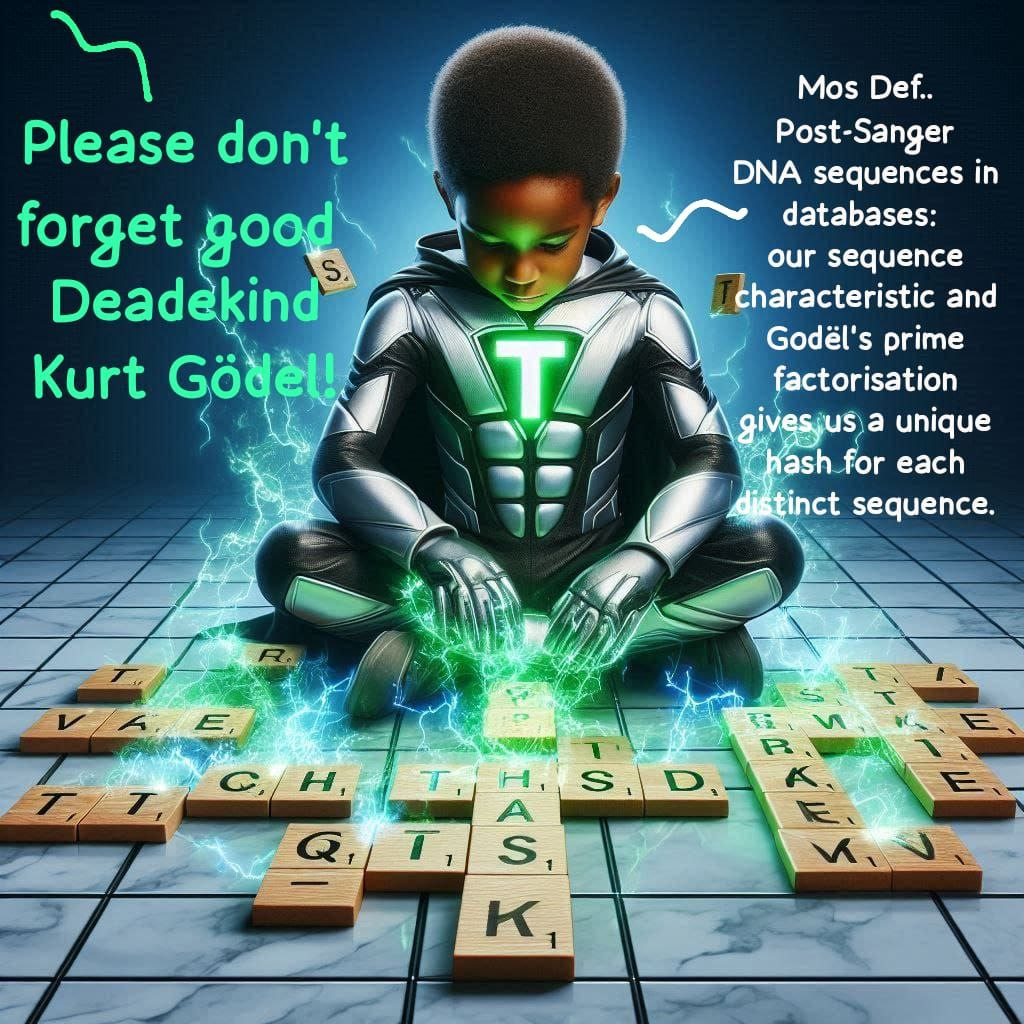
\includegraphics[width=0.9\textwidth,]{resources/images/further_analysis.jpg}\\
       \caption{Some proposal to use G$\ddot{o}$del's idea of abstracting formulae such as formal symbolic sequences using distinct natural numbers.}
      \label{FIGGODELIDEA}
    \end{figure} \\
    \cline{1-1} % Bottom border only
  \end{tabular}
\end{table}




$na$-Sequences, for which we might have a collection of them, $\Theta^n$, could have applied to them, a system of optimal or optimizable storage in practice, especially via electronic formats and protocols such as with flat text files, relative database systems and any well structured \textbf{operating memory-space structures} --- vaults in TEA\cite{Lutalo2024_taz}, JSON-dictionaries on the Web\cite{lutalo_tea_web}, YAML files on local file-systems, etc. In this section, we could explore with the same na-Sequences introduced in \textbf{\hyperref[SEC4ASEQ]{Section \ref{SEC4ASEQ}}}, for ways how their corresponding optimal hash keys might be computed as part of an optimal-sequence lookup mechanism in bio-automata or perhaps in some na-Sequence database.

Concerning Storage of a na-Sequence $\theta_i \in \Theta^n_k$ such that  $\Theta$ has $n$ sequences partitioned into $k$ subsequences\footnote{This is just the proposed concept of the storage representation for an individual entire genome sequence;  just one of many possibilities. Particular implementations might vary in actual sequence expression (in storage). For nucleic acid operating systems, we know that na-Sequences are in natural storage, when expressed as DNA (with partitions or access-abstractions able to discern individual nucleic acids, codons, genes, chromosomes, double-helixes of chromosomes, etc), however, while in use for processes such as RNA-oriented sequence processing (see \textbf{\hyperref[SECPROT]{Section \ref{SECPROT}}}), are operated on, not in bulk or whole-at-once, but in subsequences of some finite length --- such as $k$ in this formal specification, and $k=3$ for typical, natural protein synthesis in ribosomes as an example.} --- essentially, a higher-order sequence\index{sequence!higher-order}.

We then might wish to have some mechanism --- such as the following generator:

\vspace{1em}
\begin{transf}[A \textbf{Sequence Lookup System}, sLS($Q_m,\Theta^n$)\index{generator!Sequence Lookup System}]:
\label{TRANSFSEQLOOKUP}
$ $\\
$\Theta^n \xrightarrow{sLS(Q_m,\Theta^n)} \theta_i;$\\ 
$\invpi(Q_m) = m \leq \invpi(\theta_i) \quad \land \quad (\ddot{o}(Q_k) \approx \ddot{o}(\theta_i) \quad \lor \quad \tilde{A}(\overset{>}{Q_k} \rightarrow \overset{>}{\theta_i}) \leq \epsilon)$\\
$\qed$
\end{transf}
\vspace{1em}


By \textbf{\hyperref[TRANSFSEQLOOKUP]{Transformer \ref{TRANSFSEQLOOKUP}}}, we can search for and express or return, a complete na-Sequence $\theta_i \in \Theta^n$, when presented with some query na-sequence $Q_m$ of length $m$.

Thus, for optimal lookup mechanisms --- concerns about space and [polynomial] time for looking up and returning $\theta_{na}$ from some \textbf{na-database}, $D\langle {\theta i}_{key}, {\theta i}_{val} \rangle^*$, such that, instead of directly searching the collection for the sequence with value $\theta_i = {\theta i}_{val} \approx Q_m$, directly/naively using $Q_m$ --- the \textbf{user provided query}, we use the provably shorter --- in terms of storage space, but also [\textit{more intelligent-friendly} --- in terms of sequence-expressing-information] higher \textbf{entropy encoding} structure\index{sequence entropy}, such as with a \textbf{hash key} for each $\theta_i$ as well as any $Q_k$, computed as:

\vspace{1em}
\begin{equation}
\label{EQHASHKEYSEQ}
 \Gamma (id(\theta_i)) = \ddot{o}(\prod\limits_{\omega_i,f_i \in \hbar(\overset{>}{\theta_i})} \omega_i\cdot f_i) \quad \cong \quad \ddot{o}(\hbar(\overset{>}{R_{\Theta^n_k}}))
\end{equation}
\vspace{1em}



 --- see definition of $R_{\Theta^n_k} \approx \Theta_n$ in \textbf{\hyperref[LAWGDL]{IGS Law}} (\textbf{\hyperref[SECIGSL]{Section \ref{SECIGSL}}}), while the special sequence operator $\ddot{o}(\Theta_n)$ computes and returns a \textbf{G$\ddot{o}$del Number}\cite{illingworth1996computing}\footnote{Based on the concept of \textbf{G$\ddot{o}$del numbering}\index{G$\ddot{o}$del number} --- ``A one-to-one mapping (i.e. an injection) of the symbols, formulas, and finite sequences of formulas of the formal system onto some subset of the natural numbers. The mapping must be such that there is an algorithm that, for any symbol, formula, or finite sequence of formulas, identifies the corresponding natural number; this is the \textit{G$\ddot{o}$del number} of that object."\cite{illingworth1996computing}. G$\ddot{o}$del numbers are a method developed by Kurt G$\ddot{o}$del in 1931\cite{godel1931} to encode symbols, formulas, and entire proofs from formal mathematical systems as unique natural numbers. This encoding allows syntactic objects to be treated arithmetically\cite{godel1931english}.}, $\ddot{o}(\Theta_n): \psi_{\Theta_n}^k \times\mathbb{N}^k \rightarrow \mathbb{N}$ that is derived optimally using the characteristic, $\hbar(\overset{>}{\Theta_n})$, for $\Theta_n$ a sequence of length $n$, and the first $k$ prime numbers such that $k = \invpi(\overset{>}{\Theta_n}) \quad \land \quad \forall \omega_i \in \hbar(\overset{>}{\Theta_n}): \ddot{o}(\omega_i) : \ddot{o}(i) = f_i \times (p_i \in \mathbb{P})$ --- $p_i$ is the $i$-th prime\footnote{$\mathbb{P}$ is the set of all prime numbers.} starting from 2 and spanning $\mathbb{N}$.
 

Computing a hashkey based on a G$\ddot{o}$del number is just one approach to the optimal way to implement a sequence lookup mechanism with \textbf{\hyperref[TRANSFSEQLOOKUP]{Transformer \ref{TRANSFSEQLOOKUP}}}. Among the \textbf{attractive properties} of this method, is the realization that, unlike the case of using the \textbf{ADM}, the G$\ddot{o}$del number approach boils down to comparing sequences using pure numbers and to which mere basic arithmetic tests can be applied than using sequences directly or sequence projections (themselves still potentially non-numeric sequences) to which we can not readily apply search or measurements by pure arithmetic means.
 
 
 Also, note that, with the G$\ddot{o}$del number approach, and if we proceed to compute the identifier or hash-key of some sequence $\Theta$ --- i.e $\Gamma (id(\Theta))$ --- via computation of its corresponding G$\ddot{o}$del number, $\ddot{o}(\Theta) \in \mathbb{N}$, as per the following formulation:
 
 \vspace{1em}
\begin{equation}
\label{EQHASHKEYSEQGODEL}
 \Gamma (id(\Theta)) = \ddot{o}(\Theta) = \prod\limits_{f_i \in \hbar(\overset{>}{\Theta})} f_i \times p_i
\end{equation}
\vspace{1em}

So that, if we have any two sequences, $Q$ and $\Theta$, and that we wish to establish if they are potential neighbors, or symbolically related, one possibility, and a very simple technique of elimination, would be that, if we trust that the length of either $Q$ or its symbol set $\psi(Q)$ is shorter than that of the target sequence $\Theta$ --- i.e if $\invpi(Q) \leq \invpi(\Theta)$ or better, that $\invpi(\psi(Q)) \leq \invpi(\psi(\Theta)) \leq \invpi(\Theta)$, then, it would save lots of processing time, if we merely compute the symbol set of the short query, $\psi(Q)$, and from that, compute the G$\ddot{o}$del numbers of each of the query symbols, i.e $\ddot{o}(\omega_i)$ --- which assumes that for any distinct $\omega_i \in \psi(Q)$ or $\omega_i \in \psi(\Theta)$, we have a consistent method of assigning corresponding G$\ddot{o}$del numbers (for example, by ensuring that we map from $\omega_i \in \psi_* \rightarrow p_i \in \mathbb{P}$ for $\psi_* \supset \psi(Q) \cup \psi(\Theta) \quad \forall Q, \Theta$), such as via $\ddot{o}(\omega_i) = p_i : I(\omega_i, \psi_*) = I(p_i, \mathbb{P})= i$ --- and so that, via the property:


  \vspace{1em}
\begin{equation}
\label{EQHASHKEYSEQGODELTEST}
 \Gamma (id(\Omega)) \mod \ddot{o}(\omega_i) = 0 \quad \forall \omega_i \in \psi_* \cap \psi(\Omega)
\end{equation}
\vspace{1em}

We know that if any two sequences have some uncommon symbol, then we shall find that the corresponding G$\ddot{o}$del number for that symbol cannot be a factor of one of these sequences's corresponding G$\ddot{o}$del number-based identifier or hash-key. Otherwise, two sequences sharing the same symbol set shall always be guaranteed to have common G$\ddot{o}$del number factors for each of their common symbols and corresponding database hash-keys or identifiers, and thus, we can leverage this criteria to quickly eliminate unlikely candidates in a proximity or similarity lookup test for a database or other high-density sequence storage system via leveraging \textbf{a basic arithmetic modulo operation test} instead of other expensive proximity or similarity tests\index{G$\ddot{o}$del number!sequence similarity test}.
 
 
   However, even that method utilizes the transformatics concept of summarizing arbitrary sequences by their \textbf{sequence characteristic} first, and consequently, their \textbf{modal sequence statistic}, so as to later arrive at the pure number hash keys\footnote{\textbf{FUTURE WORK}: In later analyses and perhaps further development of this idea, it might help to ascertain whether or not projecting arbitrary sequences to pure numbers would still internally preserve useful distance heuristics such as how the ADM can hint at sequences that are quantifiably and especially lexically similar/close to each other, while, with G$\ddot{o}$del numbers, we have not clearly or robustly explored all such nuances, and there could be a possibility that perhaps, unless, as we have somewhat constrained our derivation methods here, it might be possible to arrive at multiple pure numbers for the same exact sequence when the formulation for computing a sequence's  G$\ddot{o}$del number is altered across storage or sequence look-up systems.}. However, as we see in the constraints and specification of that generator-transformer, the other option is to compute the solution using the ADM applied to keys based on just the modal sequence statistics of the query and the target sequences in $\Theta^n$ as we have already gotten well acquainted with in much of this chapter.
   
   Finally, given that the hashkey or identifier key for some sequence $\Theta$ as per the G$\ddot{o}$del number method might result in a potentially large natural number that is derived from the product of several natural numbers ($f_i$) and prime numbers ($p_i$), as per \textbf{\hyperref[EQHASHKEYSEQGODEL]{Equation \ref{EQHASHKEYSEQGODEL}}}, of course, unless a clever method for keeping these keys short is enforced\footnote{Such as, when for starters, we limit our sequence alphabets to only a minimal finite symbol set such as $\psi_{na}$, $\psi_{az}$ or perhaps for arbitrary text sequences, something like either $\psi_{36}$ or the ascii character set, $\psi_{ascii}$.\index{$\psi_{ascii}$}, since, by having a small alphabet or symbol set, also the corresponding largest prime number, $p_i$, that we would encounter when computing the corresponding G$\ddot{o}$del number-based keys would be thus constrained --- especially since for any such symbol set, we want to ensure that $I(\omega_1,\psi_*) = I(p_1,\mathbb{P})$ where we know that $p_1 = 2, p_2 = 3, p_3= 5, \cdots$}, otherwise, given what we know of the way that the length of number expressions grow in sequence cardinality\index{sequence!cardinality under multiplication}\index{GTNC} under multiplication for pure numbers\cite{Lutalo2024gtnc}:
   
   \vspace{1em}
   \fbox{\begin{minipage}{0.9\textwidth}
\large
\textbf{NOTE:}\\


\begin{theo}[\textbf{Cardinality under Multiplication for Pure Numbers}]
\label{T10}
Given any two \textbf{pure numbers} $\tau$ and $\sigma$, the cardinality of their product $\invpi(\tau \times \sigma)$ is bounded thus\footnote{Note that in this reformulation of \textbf{Theorem 15} of GTNC\cite{Lutalo2024gtnc}, that we have replaced use of the original cardinality notation $C_{\Theta}$ in favor of the new, transformatics notation $\invpi(\Theta)$, but the concepts and underlying logic remain the same.}

\begin{equation}
\label{EQ21}
Max(\invpi(\tau),\invpi(\sigma)) \leq \invpi(\tau \times \sigma) \leq \invpi(\tau) + \invpi(\sigma)
\end{equation} 

iff $\tau \neq 0$ and $\sigma \neq 0$ otherwise

\begin{equation}
\label{EQ21.1}
\textbf{$C_{\tau \times \sigma}$} = 1
\end{equation}

\end{theo}

\end{minipage}}
   \vspace{1em}
   
It means that for hashkeys generated via \textbf{\hyperref[EQHASHKEYSEQGODEL]{Equation \ref{EQHASHKEYSEQGODEL}}}, the size of the resulting expressions is bounded thus:

\vspace{1em}
\begin{equation}
\label{EQ21}
Max(\invpi(f_i), \invpi(p_i)) \leq \invpi(\Gamma (id(\Theta))) \leq \sum \invpi(f_i) + \invpi(p_i)
\end{equation}
\vspace{1em}

For all $f_i \geq 1$ --- which is all $f_i$ we shall encounter for any sequence, since there is no way a symbol's frequency entry, $f_i$ --- for say some $\omega_i \in \Theta$ or from an associated symbol set,  $\omega_i \in \psi_*$ --- would end up in our G$\ddot{o}$del number formulation (\textbf{\hyperref[EQHASHKEYSEQGODEL]{Equation \ref{EQHASHKEYSEQGODEL}}}) unless it at least corresponded to at minimum one symbol instance in the underlying sequence $\Theta$ and thus at least $f_i = 1$ in the corresponding $\hbar(\overset{>}{\Theta})$.



\chapter{The Mathematics of Genome Sequencing: Sequence Alignment, The Modal Sequence, The Sequencing Machine and the Identifier Genome Sequence Law}
\label{SECMATHSEQ}



\section{Relevant Background}

\begin{figure}[h]
\fbox{\begin{minipage}{0.9\textwidth}
\large
\textbf{NOTE:}\\
 On \textbf{Sequencing} \\

It is important that we have some general appreciation of the core concept about which this chapter is dedicated; \textit{sequencing}. For this matter, we shall want to bring to mind one of the popular definitions of the term as employed in computer science for example:


\begin{quotation}
\noindent \textbf{Sequencing}\index{sequencing} \texttt{The procedure by which ordered units of data (octets or messages) are numbered, transmitted over a communications network (which may rearrange their order), and reassembled into the original order at their destination.}\\
\hspace*{\fill} --- \textbf{Oxford Dictionary of Computing}\cite{illingworth1996computing}
\end{quotation}


That is the closest concept or definition I could glean from my collection of academic literature and books in my private library at Nuchwezi Research Lab, however, this other definition, obtained via Microsoft's Copilot might also help shed more light on the particular concept of concern here: \textit{genome sequencing}\index{genome sequencing}:

\begin{quotation}
\noindent \textbf{Genome Sequencing}\footnote{Also see: \url{https://en.wikipedia.org/wiki/Whole_genome_sequencing}}\cite{CDC2024GenomicSequencing}: {\ttfamily Genome sequencing is the process of determining the complete DNA (or RNA) sequence of an organism’s genome. It identifies the precise order of nucleotide bases (A, T, C, G) across all or most of the genetic material, providing a comprehensive "blueprint" of the organism's hereditary information. This technique is fundamental in biology, medicine, and biotechnology, enabling insights into genetic variation, disease mechanisms, and evolutionary relationships.

}
\hspace*{\fill} --- \textbf{Microsoft Copilot}\cite{copilot_dna_assistant}
\end{quotation}


\end{minipage}}
\end{figure}
%\vspace{2em}


First, we shall mostly assume there is essentially no reliable mathematical formalisms or theory concerning the important matter of genome sequencing\footnote{For those that do not know, a formal definition is presented in \textbf{\hyperref[DEFGENOMESEQUENCING]{Definition \ref{DEFGENOMESEQUENCING}}}.}\index{sequencing}\index{genome!sequencing}. And so, shall set out to construct and develop such a formalism ourselves, from what we already know.

Second, from the theoretical and exploratory reviews we have conducted leading up to this moment, and what some authorities\cite{przytycka_wgs_lecture10} say about the subject, we know that genome sequencing as a practice leveraging computational and mathematical principles and concepts, or rather, when approached from a predominantly mathematical theory perspective, still has some ambiguities and unresolved problems that we have identified and intend to iron out especially in this chapter.

These for example include an overall lack of proper mathematical formalisms around  issues such as:

\begin{enumerate}
\item How [genome] sequencing works or what it is exactly; how can it be described computationally?
\item If we treat of genome sequencing using the language of transformatics, and think of it in terms of processing some collection of sequences to arrive at some resultant genome sequence, how should one arrive at such a resultant sequence then? 
\item What is a ``consensus sequence"\cite{przytycka_wgs_lecture10}?
\item What is meant by ``a most representative genome sequence" or perhaps an identifying \textbf{na-Sequence} given some living organism or particular aspects of it?
\item Could we (perhaps conceptually, or theoretically) talk of sequencing a population instead of an individual organism, an entire species or perhaps (sic) non-living things too? How?
\item Could we pin down a genome sequence or some na-Sequence responsible for say the expression\footnote{Related, but not to be treated of in this chapter but instead in \textbf{\hyperref[SEC4]{Chapter \ref{SEC4}}}, is the matter of mathematically approaching how the expression --- visual, material or spatial, of any meaningful \textit{genome} sequence --- could be for a basic organism, an aspect of it, or even the case of \textit{anomalous entities} such as viruses, mere proteins or such, could be approached.} of some particular protein, some genetic mutation, a behavioral trait, anatomical or psychological anomalies and pathologies, the material basis of particular or general diseases, incapacities, etc. using a mathematical theory or language? How?
\end{enumerate}

Seeing as the matter of determining the actual na-Sequence that correctly identifies a person or thing might be hinging on the case of attempting to reconstruct a book by mathematically piecing together disparate pieces of it --- some in alignment, some out of alignment, some, supersets of  others, some prefixes or suffixes of others, etc.\footnote{This analogy shouldn't come as a surprise, when compared to how we found it best to describe DNA using a figurative metaphor (see \textbf{\hyperref[SEC1]{Introduction}}), but also based on how some authorities seem to be teaching this subject to their students\cite{przytycka_wgs_lecture10}.}, we then start to come to some appreciation of how best we might approach the problem's solution. 


Also, though we might not immediately surface such philosophical speculations here, the difficulties and problems thus raised above, might likewise apply to or at least hint at the challenges there might be, in attempting to think of or practically resolve the matter of ``computationally sequencing anything" --- the idea being, to not limit the concept of \textit{sequencing} to only living things or living organisms only, but to also think generally and abstractly \textbf{concerning sequencing anything expressible in consensus reality via some kind of specification sequence}\footnote{Or perhaps an ``identifying sequence".}. 


Thus, we might want to also think of, keep in mind, the possibility of sequencing the peculiar, miniscule aspects of consensus reality --- sub-atomic particles that make up atoms that make up molecules that make up living things on the miniature scale, and then all the way up to planets, stars and galaxies on the grand, cosmic and universal scale. One might wonder, and correctly so, is such sequencing possible? Does it/would it make sense? Is it necessary or even useful? These, and related problems are among the concerns we shall attempt to address in the rest of this chapter, but also, bits of what we can not immediately answer, perhaps we shall tackle in later chapters or future works\footnote{\textbf{FUTURE WORK:} Explore, philosophically, but also mathematically, whether or not it makes sense to think of the [genome] sequencing of arbitrary things; not necessarily only living/biological entities, but also any coherent material entities such as particular atoms, molecules,... all the way to entire ecosystems, planets and star-systems perhaps! For example, given that the manifestation of biological lifeforms on some particular planets within a star system heavily relies on some initial conditions inherent in the early formation of the star [system] itself, could it be that something fundamental in matter could underlie all manifestation or expression of existence other than just biological life, and that we might somehow be able to pin it down to some kind of identifier sequence? A genome for en entire planet or star system?}.

\section{3 Core Problems to Solve}
\label{SEC3COREPROB}

We shall develop our theory in bits, starting with the most basic, most fundamental, and then basing on that, to construct higher aspects of the necessary mathematical structures and system.

The method is simple; we have distilled 3 core problems whose solutions would culminate in the formal and mathematical definition of genome sequencing. The 3 problems are\index{genome sequencing!underlying problems}


\begin{enumerate}
\item \textbf{PROBLEM 1}: Computing the best or rather correct common subsequence given any two or more potentially dissimilar sequences.
\item \textbf{PROBLEM 2}: Computing the correct sequence that resolves conflicts and correctly expresses variations at each particular position (essentially a column) in the alignment matrix depicting a definite side-by-side alignment of two or more sequences with an overlap in the alignment position being considered.
\item \textbf{PROBLEM 3}: Computing the Genome Sequence.
\end{enumerate}

We shall tackle each of these problems in its own section, one by one, until we arrive at the original objective of this chapter, in \textbf{\hyperref[SECGENSEQ]{Section \ref{SECGENSEQ}}}.

\subsection{PROBLEM G1: Computing Maximum Common Subsequence: $\Theta_1 \Diamond \Theta_2$}
\label{PROBG1}

\begin{prob}[\textit{Computing MCS:}\index{Maximum Common Subsequence (MCS)}]: $\Theta_1 \Diamond \Theta_2$] 
\label{PROBMCS}
Given sequences $\Theta_1 = \langle k, l, m, o, p, x, y, z \rangle$ and $\Theta_2 = \langle b, c, a, y, z, k, l, m, o, p \rangle$, find the longest common subsequence they share --- also to be denoted $\Theta_1 \Diamond \Theta_2$, their \textbf{M}aximum \textbf{C}ommon \textbf{S}ubsequence.

\vspace{1em}
\begin{soln}
\label{SOLMCS}
We shall specify a transformer, tMCS($\Theta_1,\Theta_2$) that produces the required solution from the input sequences as such:

\begin{transf}[The \textbf{tMCS} Transformer\index{transformer!tMCS, for maximum common subsequence}]
\label{TRANSFMCS}
$\langle \Theta_1,\Theta_2 \rangle  \quad \xrightarrow{O_{tMCS}(\Theta_1,\Theta_2)} \quad \Theta_1 \Diamond \Theta_2;$\\
$\Theta_1 \Diamond \Theta_2 = \Theta_2 \Diamond \Theta_1$
$\quad \land \quad 0 \leq \invpi(\Theta_1 \Diamond \Theta_2) \leq Max(\invpi(\Theta_1), \invpi(\Theta_2))$\\
$\land \quad \forall \omega \in \Theta_1 \Diamond \Theta_2 \quad \exists \omega \in \Theta_1 \land \exists \omega \in \Theta_2$\\
$\land \quad \forall \omega_i, \omega_j \in \Theta_1 \Diamond \Theta_2 : I(\omega_i, \Theta_1 \Diamond \Theta_2) < I(\omega_j, \Theta_1 \Diamond \Theta_2) \quad $\\
$\quad \implies \quad I(\omega_i, \Theta_1) < I(\omega_j, \Theta_1) \quad \land \quad I(\omega_i, \Theta_2) < I(\omega_j, \Theta_2)$\\
$\land \quad \forall \Theta_1 \Diamond \Theta_2, \quad \Theta_1 \Diamond \Theta_2 \subset \Theta_1 \quad \land \quad \Theta_1 \Diamond \Theta_2 \subset \Theta_2$
\end{transf}
$\qed$
\end{soln}
\end{prob}
\vspace{1em}

\textbf{\hyperref[SOLMCS]{Solution \ref{SOLMCS}}} is easier said than done. However, we shall attempt to formally and rigorously express it by formalizing what exactly the $tMCS(\Theta_1,\Theta_2)$ transformer does when expressed as a computable algorithm. Basically, we are to compute the MCS via \textbf{\hyperref[ALGtMCS]{Algorithm \ref{ALGtMCS}}} specified hereafter.

\vspace{2em}
\begin{alg}[The \textbf{tMCS} Algorithm\index{algorithm!computing MCS}\footnote{\textbf{IMPORTANT:} Note that, even though the MCS transformer, \textbf{\hyperref[TRANSFMCS]{Transformer \ref{TRANSFMCS}}}, is defined for just two sequences, and yet, the tMCS algorithm based off of it is designed to handle any arbitrary number of sequences and not just a pair.}]
\label{ALGtMCS}
$ $
\begin{enumerate}
\item{\textbf{INITIALIZE} the global maximum common sequence, $O^m_g$, to the empty sequence\footnote{Refer to \textbf{\hyperref[RES1]{Foundation Idea \ref{RES1}}}}.} 
\item{
\textbf{GIVEN}  \textbf{a collection of $n$ sequences}, $\Theta^n = \{\Theta_1, \Theta_2,..., \Theta_n\}$.
}
\item{
\textbf{START}  by computing the cardinality of each sequence, $\Theta_i \in \Theta^n$, and note the \textbf{largest sequence cardinality}, $Max(\invpi(\Theta_i) \quad \forall \Theta_i \in \Theta^n)$ = $Max(\invpi(\Theta_i))$, for the longest sequence, $\Theta_m$ such that $Max(\invpi(\Theta_i)) = \invpi(\Theta_m)$.
}
\item {
\textbf{COMPUTE}  the cardinality of a sequence that can exactly contain the given sequences each concatenated to the other, but with the longest sequence duplicated. Essentially, compute:

\begin{equation}
\label{EQLSEQ}
C_R = \invpi(\Theta_m) + \sum\limits_{\forall \Theta_i \in \Theta^n} \invpi(\Theta_i)
\end{equation}

}
\item{
\textbf{SORT}  the collection of sequences, $\Theta^n$, in descending order\footnote{\textbf{FUTURE WORK:} We especially prefer descending order by sequence cardinality because, as we shall come to appreciate in the rest of the tMCS algorithm, it is more likely that the MCS is discovered or developed based on the longest  common [sub-]sequence (in the longest sequences in the collection) than if we had started out with the shortest sequences. In fact, it also is somewhat very logical, since, the longest sequence shall most likely also contain elements and subsequences that shorter sequences have or are derived from than vice versa! Thus we can converge towards the MCS faster that way. Also, this is \textit{the optimistic strategy} --- believing that the most common subsequence shall most likely already exist in the longest sequences we are analyzing --- which makes sense for genome sequencing given we are typically analyzing sequences from the same entity or individual or species, and that DNA or genetic code for the same individual or entity stays consistent across all or most of the samples from that entity. But otherwise the pessimist route might be to start out with the shortest sequences in the collection (esp. where we are dealing with totally antagonistic entities). But is this always optimal? Should it stay this way even when we are attempting [genome] sequencing for non-biological or non-genetic sequences?} of the sequence cardinality. Let the sorted sequence collection be denoted ${\hat{\Theta}}^n = \langle \Theta_m, \Theta_{2*}, \cdots , \Theta_{n*} \rangle$ --- where the first item in ${\hat{\Theta}}^n$, $\Theta_{1*}$ is essentially $\Theta_m$.
}
\item{
\textbf{SELECT}  the first two sequences from ${\hat{\Theta}}^n$, such as  $\Theta_m$ and $\Theta_{2*}$ --- or rather/generally, ${\hat{\Theta}}^n[1]$ and ${\hat{\Theta}}^n[2]$, as the two sequences we shall use to search for and derive the potential MCS.
}
\item { \textbf{POSITION} the two sequences, $\Theta_m$ and $\Theta_{2*}$ within two adjacent arrays $A_1^{C_R}$ and $A_2^{C_R}$ of equal length $C_R$ --- for simplicity, we shall just denote them as  $A_1$ and $A_2$, in such a way that $\Theta_m$ occupies in its containing array $A_1$, positions from m to $2m$, but for simplicity's sake\footnote{We shall later see (in \textbf{Step\#8(c)}) that it is useful to position $\Theta_m$ this way, because then, the second sequence's positions are all that need to be changed --- items being shifted leftwards in $A_2$ relative to $A_1$, while those of the longest sequence in $A_1$ remain fixed. But to keep the mathematical formalisms simple, we shall especially write our expressions as though elements of $\Theta_m$ were positioned from index 1 in $A_1$ --- these details especially matter to programmers and software engineers that shall want to translate the algorithm into working computer program source-code for various different languages and type-systems.}, which we shall just treat as though 1 to $m$:

\vspace{1em}
 $A_1: [1, m]$
\vspace{1em}


While $\Theta_{2*}$ occupies positions in the range\footnote{We write ``$\Theta_{2*}[1]$" in our formulation here, to mean the first element in $\Theta_{2*}$ --- i.e. position 1 has value 1, and the nth position has value $n$, not usual (computer-science) $n-1$}:

\vspace{1em}
 $A_2: [(1 + I(\Theta_m[m], A_1)$, $\quad$ $I(\Theta_m[m], A_1) + \invpi(\Theta_{2*})]$
\vspace{1em}

Or, equivalently, the range:

\vspace{1em}
$A_2: [m+1,\quad m + \invpi(\Theta_{2*})]$. 
 \vspace{1em}

Which we can also express visually as:\\\\

\begin{tabular}[H]{|c||c|c|c|c|c|c|c|c|c|c|}
\hline
$A_1$ & $\cdots$ & $a_{1,1}$ & $a_{1,2}$ & $\cdots$ & $a_{1,m}$ & & & & & $\cdots$\\
\hline
$A_2$ & $\cdots$ & & & & & $a_{2,1}$ & $a_{2,2}$ & $\cdots$ & $a_{2,\invpi(\Theta_{2*})}$ & $\cdots$ \\
\hline
 
\end{tabular}\\\\


}
\item{
\textbf{UPDATE}  the two sequence alignment arrays as such:
\begin{enumerate}
\item{
\textbf{KEEP}  the first array, $A_1$, unchanged (since it contains the longest sequence, $\Theta_{1*} \in \hat{\Theta}_n$).
}
\item \textbf{SET}  $j = z$, where $z$ is the \textbf{shift step size} --- simplest scenario, $z = 1$.
\item {\textbf{SHIFT}  each element in the second sequence by $j$-steps to an earlier position in array $A_2$, so that the two sequences $\Theta_m$ and $\Theta_{2*}$ have an overlap across the alignment arrays/matrix in positions spanning range:

\vspace{1em}
 $A_1: [m-j,\quad m]$
\vspace{1em}
 
and so that $\Theta_2$ shall be occupying the updated range: 

\vspace{1em}
$A_2: [m + 1 - j,\quad m+\invpi(\Theta_{2*}) - j]$
\vspace{1em}
}
\item {
\textbf{SCAN}  the overlapping sections in both sequences, in positions  $[m-j, m]$ and by comparing each item in that range --- i.e. $\Theta_m[i]$ Vs $\Theta_{2*}[i]$, determine the longest common subsequence, or rather the \textbf{MCS}, thus:\\

Assume the overlap is of length\footnote{Essentially, since the overlap spans the range $[m-j, m]$, then $\phi = m - (m-j) = j$}$\phi$ such that the overlap can be visually depicted as such:

{

\vspace{2em}
% to force wide table to fit well on page irrespective of nesting/list indentation
\begin{adjustwidth}{-4em}{}
\begin{tabular}[H]{|c||c|c|c|c|c|}
\hline
$\approx \Theta_m$ & $a_{1,m-\phi+0}$ &$a_{1,m-\phi+1}$ & $a_{1,m-\phi+2}$ & $\cdot\cdot\cdot$ & $a_{1,m-\phi+j}$\\
\hline
$\approx \Theta_2$ & $a_{2,m-\phi}$ &$a_{2,m-\phi+1}$ & $a_{2,m-\phi+2}$ & $\cdot\cdot\cdot$ & $a_{2,m}$\\
\hline
$(\Theta_m[i] == \Theta_{2*}[i])?$ & 1 & 1& 0 &  $\cdot\cdot\cdot$ & 1\\
\hline
$\approx (\Theta_m[i] == \Theta_{2*}[i]) \approx O^\phi$ & $f(\Theta_m[i],\Theta_{2*}[i])$ & $a_{1,m-\phi+1}$ & 0 &  $\cdot\cdot\cdot$ & $f(a_{1,m},a_{2,m})$ \\
\hline
 \end{tabular}
 \end{adjustwidth}
  \vspace{2em}

 }

 
 \textbf{CREATE}  another array of maximum length $\phi$, i.e. $O^\phi$, which contains at most $\phi$ elements generated thus:
 \begin{itemize}
 \item{ $O^\phi[i]$ contains 0 if the corresponding two elements in $\Theta_m$ and $\Theta_{2*}$ didn't match. Otherwise it contains the matching element value from the first sequence. Essentially, resolve what goes into $O^\phi$ at each of the overlap indices --- $i: i \in [m-\phi, m]$ ---  via the function:
 
 \vspace{1em}
\begin{equation}
f(\Theta_m[i],\Theta_{2*}[i]) = \begin{cases}
\Theta_m[i] & \Theta_m[i] == \Theta_{2*}[i],\\
0 & \Theta_m[i] \neq \Theta_{2*}[i]
\end{cases}
\end{equation}
 \vspace{1em}
 
 
 }
 \item \textbf{TRUNCATE}  $O^\phi$ to its longest non-zero/non-empty subsequence, and \textbf{SET} that as $\bar{O^\phi}$.
 \item \textbf{IFF}  $\invpi(\bar{O^\phi}) > \invpi(O^m_g)$, then \textbf{UPDATE} or replace $O^m_g$ with $\bar{O^\phi}$\\ $\implies$  $O^m_g := \bar{O^\phi}$
 \end{itemize}
}
\item{
\textbf{UPDATE}  $j \implies j := j + z$
}
\item {
\textbf{IFF}  $j = \invpi(\Theta_m) + \invpi(\Theta_{2*})$, then \textbf{GOTO}\footnote{At this juncture, we shall have essentially finished sliding the second sequence, $\Theta_{2*}$, past all the elements of the first sequence so that at $j = \invpi(\Theta_m) + \invpi(\Theta_{2*})$ there is nomore overlap possible, and so we can move on to the next sequence.} \textbf{Step\#9}
}
\item{\textbf{ELSE} \textbf{ITERATE}  from \textbf{Step\#c}}
\end{enumerate}
}

\item{ \textbf{UPDATE} $\Theta_{2*}$ as such:

\begin{itemize}
\item{ \textbf{COMPUTE} index of next comparison sequence, $k$, as such: 

\vspace{1em}
\begin{equation}
k = I(\Theta_{2*},{\hat{\Theta}}^n) + 1
\end{equation}
\vspace{1em}

}
\item \textbf{IFF} $k > n$, then \textbf{RETURN}\footnote{Basically, we have reached the end of our sorted list of sequences and whatever we currently have as MCS must be the solution.}  $O^m_g$.
\item \textbf{ELSE} \textbf{LET} $\Theta_{2*} := {\hat{\Theta}}^n[k]$

\end{itemize}

}
\item \textbf{IFF} $\invpi(\Theta_{2*}) <  \invpi(O^m_g)$, then \textbf{RETURN}\footnote{Basically, once we find that the current MCS is longer than any of the remaining sequences in the collection, we might as well stop searching and return it as the final solution.}  $O^m_g$.
\item \textbf{ELSE ITERATE}  from \textbf{Step\#7}
\end{enumerate}


%\end{enumerate}
$\qed$
\end{alg}
\vspace{2em}

%draw horizontal line
\noindent\rule{\textwidth}{0.4pt}

\vspace{2em}

\subsubsection{Applying The Transformer and Associated Alogirithm}
\label{SECAPPLYTRANSALG}

And so, applying \textbf{\hyperref[ALGtMCS]{Algorithm \ref{ALGtMCS}}} to our example sequence collection:

We see that:

\begin{enumerate}
\item Initially, our MCS, $O^m_g = \langle \rangle$.
\item{ For our given sequences, we have our collection $\Theta^n = \Theta^2$ as such:

\vspace{1em}
\begin{equation}
 \Theta^n = \langle \Theta_1, \Theta_2 \rangle = \langle \langle k, l, m, o, p, x, y, z \rangle , \langle b, c, a, y, z, k, l, m, o, p \rangle \rangle
\end{equation}
\vspace{1em}

}
\item $\invpi(\Theta_1) = 8$, and $\invpi(\Theta_2) = 10$, so that then, $\Theta_2$ is our longest sequence, and thus $\Theta_m = \Theta_2$.
\item{ As for the size of our alignment array, we have that:

\begin{equation}
C_R = 10 + (10 + 8) = 28
\end{equation}


}
\item And as for the sorted collection, we have that $\hat{\Theta}^n = \langle \Theta_2, \Theta_1 \rangle$, which implies that initially, $\Theta_{2*} = \Theta_1$.
\item{As for how the two sequences are located in the alignment matrix or arrays, we have the following visual depiction initially:

\vspace{1em}
% to force wide table to fit well on page irrespective of nesting/list indentation
\begin{adjustwidth}{0em}{}
\begin{tabular}[H]{|c||c|c|c|c|c|c|c|c|c|c|c|c|c|c|c|c|c|c|c|}
\hline
$i$ & $\cdots$ & 1 & 2 & 3 & 4 & 5 & 6 & 7 & 8 & 9 & 10 & 11 & 12 & 13 & 14 & 15 & 16 & 17 & 18 \\
\hline
$A_1$ & $\cdots$ & b & c & a & y & z & k & l & m & o & p &  &  &  &  &  &  &  &  \\
\hline
$A_2$ & $\cdots$ &  &  &  &  &  &  &  &  &  &  & k & l & m & o & p & x & y & z  \\
\hline
 
\end{tabular}
\end{adjustwidth}
\vspace{1em}

At which point, the MCS between these two sequences, $\Theta_m \Diamond \Theta_{2*}$ = $O^\phi = \langle \rangle$.

}
\item{ We find that there shall be no interesting overlaps until when we reach $j = 5$, at which point, we shall have the following alignment configuration:

\vspace{1em}
% to force wide table to fit well on page irrespective of nesting/list indentation
\begin{adjustwidth}{0em}{}
\begin{tabular}[H]{|c||c|c|c|c|c|c|c|c|c|c|c|c|c|c|c|c|c|}
\hline
$i$ & $\cdots$ & 1 & 2 & 3 & 4 & 5 & 6 & 7 & 8 & 9 & 10 & 11 & 12 & 13 & 14 & 15 & $\cdots$ \\
\hline
$A_1$ & $\cdots$ & b & c & a & y & z & k & l & m & o & p &  &  &  &  &  &$\cdots$ \\
\hline
$A_2$ & $\cdots$ &  &  &  &  &  & k & l & m & o & p & x & y & z &  &  &$\cdots$\\
\hline
$a_1[i]==a_2[i]?$ & $\cdots$ & 0 & 0 & 0 & 0 & 0 & 1 & 1 & 1 & 1 & 1 & 0 & 0 & 0 & 0 & 0 & $\cdots$ \\
\hline
 
\end{tabular}
\end{adjustwidth}
\vspace{1em}

At which point, the MCS between these two sequences, $\Theta_m \Diamond \Theta_{2*}$ = $O^\phi = \langle k, l, m, o, p\rangle$, and that $\invpi(O^\phi) = 5 \quad > \quad \invpi(O^m_g)$, and so then we can update the global MCS so that $O^m_g = \langle k, l, m, o, p\rangle$.


}
\item{ At $j =  \invpi(\Theta_m) = 10$, we find that the second sequence shall entirely be positioned at the start of the longest sequence, and that we should have the second sequence entirely overlapping with the first, and at which point, we shall have the following alignment configuration for our example:

\vspace{1em}
% to force wide table to fit well on page irrespective of nesting/list indentation
\begin{adjustwidth}{0em}{}
\begin{tabular}[H]{|c||c|c|c|c|c|c|c|c|c|c|c|c|c|}
\hline
$i$ & $\cdots$ & 1 & 2 & 3 & 4 & 5 & 6 & 7 & 8 & 9 & 10 & $\cdots$ \\
\hline
$A_1$ & $\cdots$ & b & c & a & y & z & k & l & m & o & p &$\cdots$ \\
\hline
$A_2$ & $\cdots$ & k & l & m & o & p & x & y & z &  &  &$\cdots$\\
\hline
$a_1[i]==a_2[i]?$ & $\cdots$ & 0 & 0 & 0 & 0 & 0 & 0 & 0 & 0 & 0 & 0  & $\cdots$ \\
\hline
 
\end{tabular}
\end{adjustwidth}
\vspace{1em}

At which point, the MCS between these two sequences, $\Theta_m \Diamond \Theta_{2*}$ = $O^\phi = \langle \rangle$, and that $\invpi(O^\phi) = 0 \quad < \quad \invpi(O^m_g)$, and so then we cannot update the global MCS so that, \textbf{still}, $O^m_g = \langle k, l, m, o, p\rangle$.


}
\item{ At $j =  13$, we find that we have another interesting overlap, and at which point, we shall have the following alignment configuration for our example:

\vspace{1em}
% to force wide table to fit well on page irrespective of nesting/list indentation
\begin{adjustwidth}{0em}{}
\begin{tabular}[H]{|c||c|c|c|c|c|c|c|c|c|c|c|c|c|c|c|c|}
\hline
$i$ & $\cdots$ & 1 & 2 & 3 & 4 & 5 & 6 & 7 & 8 & 9 & 10 & 11 & 12 & 13 & 14 & $\cdots$ \\
\hline
$A_1$ & $\cdots$ & & & & b & c & a & y & z & k & l & m & o & p & &$\cdots$ \\
\hline
$A_2$ & $\cdots$ & k & l & m & o & p & x & y & z &  &  & & & & &$\cdots$\\
\hline
$a_1[i]==a_2[i]?$ & $\cdots$ & 0& 0 & 0 & 0 & 0 & 0 & 1 & 1 & 0 & 0 & 0 & 0 & 0  &0 & $\cdots$ \\
\hline
 
\end{tabular}
\end{adjustwidth}
\vspace{1em}

At which point, the MCS between these two sequences, $\Theta_m \Diamond \Theta_{2*}$ = $O^\phi = \langle y, z\rangle$, and that $\invpi(O^\phi) = 2 \quad < \quad \invpi(O^m_g)$, and so then we cannot update the global MCS so that, \textbf{still}, $O^m_g = \langle k, l, m, o, p\rangle$.


}
\item We finally stop when $j = \invpi(\Theta_m) + \invpi(\Theta_{2*}) = 10 + 8 = 18$, and at which point we shall find that we have not encountered any other overlap longer than our earlier MCS, and so that, given we also have no more sequences to compare against, we must \textbf{return the final MCS} as $O^m_g = \langle k, l, m, o, p\rangle$.
\end{enumerate}

\vspace{2em}

Thus, after applying  \textbf{\hyperref[ALGtMCS]{Algorithm \ref{ALGtMCS}}} to our two-member sequence collection, we find that the MCS solution we arrive at is $\langle k, l, m, o, p\rangle$ for that particular higher-order sequence. We can confirm that the solution conforms to the specifications of \textbf{\hyperref[TRANSFMCS]{Transformer \ref{TRANSFMCS}}}, such as noting that:

\begin{itemize}
\item From $\langle \Theta_1, \Theta_2 \rangle$, we have $\Theta_1 \Diamond \Theta_2$ = $\Theta_2 \Diamond \Theta_1$ =  $\langle k, l, m, o, p\rangle$.
\item We see that $\invpi(\Theta_1 \Diamond \Theta_2) = 5$, so that $ 0 \leq \invpi(\Theta_1 \Diamond \Theta_2) \leq Max(10, 8)$
\item We also see that all elements in $\Theta_1 \Diamond \Theta_2$ also exist in either sequences.
\item And also that the relative order of elements in $\Theta_1 \Diamond \Theta_2$ preserves the relative order of corresponding symbols in both $\Theta_1$ and $\Theta_2$.
\item And that finally, we see that $\Theta_1 \Diamond \Theta_2$ is a sub-sequence of both $\Theta_1$ and $\Theta_2$.
\end{itemize}





\subsection{PROBLEM G2: Computing Overlap Resultant Sequences: $\Theta_1 \ast \Theta_2$}
\label{PROBG2}

\begin{prob}[\textit{Computing ORS: \textbf{Overlap Resultant Sequence}}\index{Overlap Resultant Sequence (ORS)}]: $\Theta_1 \ast \Theta_2$] 
\label{PROBORS}
Given two overlapping/well-aligned sequences $\Theta_1$ and $\Theta_2$ of the same length but potentially different terms at any position in the range $[1, \invpi(\Theta_1)]$, how to compute a resultant sequence $\Theta_1 \ast \Theta_2$ that is most meaningful for DNA sequences?

\vspace{1em}
\begin{soln}
\label{SOLORS}
Assuming $\Theta_1 = \langle \prod\limits_{i=1}^n a_i, \rangle$ and $\Theta_2 = \langle \prod\limits_{i=1}^n b_i, \rangle$, construct $\Theta^*$ via the following tORS transformer:

\begin{transf}[The \textbf{tORS} Transformer\index{transformer!tORS, for Overlap Resultant Sequence}]$ $\\
\label{TRANSFORS}
$\langle\langle \Theta_1\langle \prod\limits_{i=1}^n a_i, \rangle, \Theta_2\langle \prod\limits_{i=1}^n b_i, \rangle \rangle  \quad \xrightarrow{O_{tORS}(\Theta_1,\Theta_2)} \quad \Theta^* = 	 \quad \Theta_1 \ast \Theta_2;$\\
$\invpi(\Theta_1 \ast \Theta_2) = \invpi(\Theta_1) = \invpi(\Theta_2) = n$\\
$\land \quad \Theta^* = \langle \prod\limits_{i=1}^n f(a_i,b_i), \rangle$\\
 for $f(x,y)$ \textbf{the ORS resolver function} defined as such:

\[
f(x,y) = 
\begin{cases}
x, & x == y, \text{terms are the same}\\
x, & x = \lnot(y), \text{one term is the complement of the other}\\
y & otherwise.
\end{cases}
\]

\end{transf}
$\qed$
\vspace{2em}
\end{soln}
\end{prob}

\vspace{2em}


Concerning that succinct solution, note that we have covered sequence complements in \textbf{\hyperref[SEC3A]{Chapter \ref{SEC3A}}} and especially for DNA or na-Complements\index{na-Complement!application in computing ORS} in \textbf{\hyperref[SECSIGCOMPLE]{Section \ref{SECSIGCOMPLE}}}. We shall not delve into the intricacies of translating \textbf{\hyperref[TRANSFORS]{Transformer \ref{TRANSFORS}}} into a working generic algorithm such as we did for \textbf{\hyperref[PROBG1]{Problem G1}}, because we have already well illustrated how the process works --- see or compare  \textbf{\hyperref[ALGtMCS]{Algorithm \ref{ALGtMCS}}} to \textbf{\hyperref[TRANSFMCS]{Transformer \ref{TRANSFMCS}}}, and also see how we have applied both the algorithm and underlying transformer to some illustrative test-cases in \textbf{\hyperref[SECAPPLYTRANSALG]{Section \ref{SECAPPLYTRANSALG}}}. Thus, it should not be hard for the serious student, researcher or genetics engineer to apply, verify and/or extend the above proposed solution to their particular needs.

Finally, note that being able to compute the \textbf{ORS} is quite useful, as it underlies the computation of the consensus overlapping sequence from which a genome sequence is then derivable as we see in the next section.



\subsection{PROBLEM G3: Computing the Genome Sequence (GS): $(\Theta_1 \Diamond \Theta_2)^*$}
\label{SECCOMPGENSEQ}

\begin{prob}[\textit{Computing GS: \textbf{Genome Sequence}}]: $(\Theta_1 \Diamond \Theta_2)^*$] 
\label{PROBGS}
Given any two sequences, $\Theta_1$ and $\Theta_2$, that are the elements of a sequence collection, $\Theta^n$, compute their \textbf{resultant genome sequence}\index{genome sequence}\index{genome sequence!defining problem}, denoted $(\Theta_1 \Diamond \Theta_2)^*$, that contains at core, their longest common subsequence (the MCS), $O^m = (\Theta_1 \Diamond \Theta_2)$, potentially padded on either side by the specially computed prefix and suffix subsequences from either input sequence as such:

\vspace{1em}
\begin{equation}
\label{EQGS}
(\Theta_1 \Diamond \Theta_2)^* \quad = \quad \Theta_1^a\cdot(\Theta_1^b \ast \Theta_2^b)\cdot(\Theta_1 \Diamond \Theta_2)\cdot(\Theta_1^c \ast \Theta_2^c)\cdot\Theta_2^a\\\\
\end{equation}
\vspace{1em}

And where the special terms are derived and named as such:

\begin{itemize}
\item $\Theta_1^a$ is the non-overlapping section of $\Theta_1$ before the \textbf{COS} --- to be introduced soon.
\item $(\Theta_1^b \ast \Theta_2^b)$ is a consensus sequence from $\Theta_1$ and $\Theta_2$ such that its elements are the result of applying the \textbf{ORS resolver function} to compute $f(\Theta_1[i],\Theta_2[i])$ as specified in \textbf{\hyperref[TRANSFORS]{Transformer \ref{TRANSFORS}}}. Thus, it is one of the overlapping resultant sequences (ORS) resulting from $\Theta_1$ and $\Theta_2$ --- this particular one occurring \textbf{before the MCS}.
\item $(\Theta_1 \Diamond \Theta_2)$ is the \textbf{maximum common subsequence}, MCS, $O^m_g$, of $\Theta_1$ and $\Theta_2$. It is the heart of the computed genome sequence.
\item $(\Theta_1^c \ast \Theta_2^c)$ is the other ORS from $\Theta_1$ and $\Theta_2$, this one occurring  \textbf{after the MCS}.
\item  $\Theta_2^a$ is the non-overlapping section of $\Theta_2$ after the \textbf{COS}.
\end{itemize}

\textbf{COS}, $\overline{\Theta_1\Theta_2}$, which is the \textbf{Consensus Overlapping Sequence}\index{consensus overlapping sequence}\index{consensus overlapping sequence!properties}, padded on either side by the non-overlapping sections of either $\Theta_1$ or $\Theta_2$, has the following properties:

\begin{itemize}
\item $\overline{\Theta_1\Theta_2} = (\Theta_1^b \ast \Theta_2^b)\cdot(\Theta_1 \Diamond \Theta_2)\cdot(\Theta_1^c \ast \Theta_2^c)$
\item $\Theta_1 \approx \Theta_1^a \cdot \overline{\Theta_1\Theta_2}$
\item $\Theta_2 \approx \overline{\Theta_1\Theta_2} \cdot \Theta_2^a$
\end{itemize}

So that we could rewrite \textbf{\hyperref[EQGS]{Equation \ref{EQGS}}} as such:

\vspace{1em}
\begin{equation}
\label{EQGS2}
(\Theta_1 \Diamond \Theta_2)^* \quad = \quad \Theta_1^a\cdot\overline{\Theta_1\Theta_2}\cdot\Theta_2^a
\end{equation}
\vspace{1em}

Finally, we know that the cardinality of the genome sequence, $\invpi((\Theta_1 \Diamond \Theta_2)^*)$, is bounded thus:

\vspace{1em}
\begin{equation}
\label{EQBOUNDGSa}
\invpi(\Theta_m) \leq \invpi((\Theta_1 \Diamond \Theta_2)^*) \leq C_R - \invpi(\Theta_m)
\end{equation}
\vspace{1em}

As per \textbf{\hyperref[EQLSEQ]{Equation  \ref{EQLSEQ}}} and the sensibilities of GTNC\cite{Lutalo2024gtnc}, and which inequality, in its most general form (applicable to a genome sequence derived from more than just two sequences) we might also depict as\index{genome sequence!limits on size}\footnote{\textbf{NOTE:} we write $\Diamond(\Theta^n)$ in  \textbf{\hyperref[EQBOUNDGSb]{Equation  \ref{EQBOUNDGSb}}} instead of $\Theta_1 \Diamond \Theta_2$ to mean the MCS resulting from processing all (potentially more than just two) sequences in some collection or higher-order sequence $\Theta^n$. And so that, even though it results from a higher-order sequence,$\Diamond(\Theta^n)$, just like $\Theta_1 \Diamond \Theta_2$, is a first-order (or rather, ``flat") sequence\index{first-order sequence}.}:


\vspace{1em}
\begin{equation}
\label{EQBOUNDGSb}
Max(\invpi(\Theta_i)) \leq \invpi(\Diamond(\Theta^n)) \leq \sum\limits_{\forall \Theta_i \in \Theta^n} \invpi(\Theta_i)
\end{equation}
\vspace{1em}


\end{prob}

\section{The Genome Sequencer}
\label{SECGENSEQ}

\fbox{\begin{minipage}{0.9\textwidth}
\begin{defn}[A \textbf{Genome Sequencer}]
\label{DEFGENOMESEQ} 
A solution to \textbf{\hyperref[PROBGS]{Problem \ref{PROBGS}}}, is a special sequence processor, $\tilde{T}(\Theta^n)$, that can compute and return a resultant sequence, $R_{\Theta^n}$, also known as the \textbf{genome sequence}, defined as\footnote{Note that in our formalism here we express the \textbf{sequence difference} of $\{\Theta_m\}$ from $\Theta^n$ as $\Theta^n \setminus \Theta_m$ --- essentially using a set-theoretic notation even though we are actually dealing with sequences here. This, so as to keep the notation simple, but otherwise, later also appeal to the same concept when considering the remaining higher-order sequence after the first $j$ member sequences have been processed and removed from it, with the notation $\Theta^{n-j}$.}

\vspace{1em}
\begin{equation}
\label{EQGSVAL}
R_{\Theta^n} = (\Theta_m \Diamond (\hat{\Theta}^n \setminus \Theta_m))^* 
\end{equation}
\vspace{1em}

Such that $\Theta_m$ is the longest sequence in $\Theta^n$ --- a collection of $n$ sequences or $\hat{\Theta}^n$, its version with member sequences sorted in descending order of sequence cardinality, and that $\tilde{T}(\Theta^n)$ produces/generates/computes $R_{\Theta^n}$ by iteratively computing and updating the genome sequence in n-1 iterations over $\hat{\Theta}^n$ as such\index{transformer chain}

\vspace{1em}
\begin{trans}
\label{TRANSGENSEQ}
$R_{\hat{\Theta}^n}^0 \xrightarrow{O_{tGS}(R_{\hat{\Theta}^n}^0,\hat{\Theta}^{n-1},1)} R_{\Theta^n}^1$
$\xrightarrow{O_{tGS}(R_{\hat{\Theta}^n}^1, \hat{\Theta}^{n-2},2)} R_{\hat{\Theta}^n}^2$
$\xrightarrow{O_{tGS}(R_{\hat{\Theta}^n}^2, \hat{\Theta}^{n-3},3)} R_{\hat{\Theta}^n}^3$
$\ldots \xrightarrow{O_{tGS}(R_{\hat{\Theta}^n}^{j-1}, \hat{\Theta}^{n-j},j)} R_{\hat{\Theta}^n}^{j+1}$
$\ldots \xrightarrow{O_{tGS}(R_{\hat{\Theta}^n}^{n-2}, \hat{\Theta}^{1},n-1)} R_{\hat{\Theta}^n}^{n}$
\end{trans}
\vspace{1em}

To produce the final genome sequence, $R_{\hat{\Theta}^n}^{n}$ via the \textbf{tGS Transformer} defined as such:

\vspace{1em}
\begin{transf}[The \textbf{tGS Transformer}, $\tilde{T}(\Theta^n)$\index{transformer!tGS, Genome Sequencer}\index{genome sequencer}]
\label{TRANSFGENSEQ}
$ $\\
$R_{\hat{\Theta}^n}^{j}  \xrightarrow{O_{tGS}(R_{\hat{\Theta}^n}^{j-1}, \hat{\Theta}^{n-j},j)} R_{\hat{\Theta}^n}^{j+1};$\\
$R_{\hat{\Theta}^n}^{0} = \Theta_m \quad \land \quad R_{\hat{\Theta}^n}^{j+1} = ( R_{\hat{\Theta}^n}^j \Diamond \hat{\Theta}^{n-j}[1])^* \quad \forall j \geq 1$\\
$\qed$
\vspace{1em}

and $R_{\hat{\Theta}^n}^{j+1}$ is the resultant genome sequence after processing $\hat{\Theta}^n$ with the first $j$ sequences removed from it, and with the previous genome sequence, $R_{\hat{\Theta}^n}^j$ passed to it, as the current best candidate genome sequence so as to produce that next genome sequence $R_{\hat{\Theta}^n}^{j+1}$. Also, for a sequence collection of $n$ member sequences, we write $R_{\Theta^n}$ to also mean $R_{\hat{\Theta}^n}^{n}$ as in \textbf{\hyperref[EQGSVAL]{Equation \ref{EQGSVAL}}}.
\end{transf} 
\vspace{1em}

\end{defn}
\end{minipage}}
\vspace{2em}

Thus, \textbf{\hyperref[TRANSFGENSEQ]{Transformer \ref{TRANSFGENSEQ}}}, $\tilde{T}(\Theta^n)$, is a genome sequencer, and is essentially a transformer that reduces a matrix of na-Sequences to a resultant sequence, $R_{\Theta^n}$, that is the resultant genome sequence of a specie, population, or any natural entity\footnote{In principle though, it is not that we can not apply this theory to the computing of genome sequences for artificial or rather conceptual entities too.} represented by or expressed by the [potentially incomplete or approximate] genome sequences in the collection $\Theta^n$.

It shall be worth noting that, for the special case where we merely have a collection of just two sequences from which to compute the genome --- such as when $\Theta^n = \langle \Theta_1, \Theta_2 \rangle $ for some two [na-]sequences, $\Theta_1$ and $\Theta_2$, we shall readily find that applying \textbf{\hyperref[TRANSFGENSEQ]{Transformer \ref{TRANSFGENSEQ}}} to that pair of sequences reduces to the case we have encountered in \textbf{\hyperref[PROBGS]{Problem \ref{PROBGS}}}, and that then, we find that:

\vspace{1em}
\begin{equation}
R_{\Theta^n} = (\Theta_m \Diamond (\hat{\Theta}^n \setminus \Theta_m))^* \quad = \quad (\Theta_1 \Diamond \Theta_2)^* \quad = \quad \Theta_1^a\cdot\overline{\Theta_1\Theta_2}\cdot\Theta_2^a
\end{equation}
\vspace{1em}


Finally, it shall help to put it out clearly, what our working definition of \textbf{Genome Sequencing} is, given what we now know.

\vspace{1em}
\begin{center}
\fbox{\begin{minipage}{0.9\textwidth}
\begin{defn}[\textbf{Genome Sequencing}\index{genome sequencing}]
\label{DEFGENOMESEQUENCING} 

When a collection of na-Sequences, $\Theta^n$, is reduced to a single na-Sequence, $\Theta_{gs}$, via a process that correctly aligns all the sequences in $\Theta^n$ such that the resultant $\Theta_{gs}$ is the best representative consensus sequence given all the variations in $\Theta^n$, we call $\Theta_{gs}$ the \textbf{genome sequence} of $\Theta^n$, and we know that if some other sequence, $\Omega_{na}$ is considered to be a legitimate genome sequence of $\Theta^n$, then it must be equivalent to $\Theta_{gs}$, where $\Theta_{gs}$ can be computationally produced from $\Theta^n$, via \textbf{\hyperref[TRANSFGENSEQ]{Transformer \ref{TRANSFGENSEQ}}} as such:


\begin{trans}
$\Theta^n  \xrightarrow{\tilde{T}(\Theta^n)} \Theta_{gs}$
\end{trans}

and equivalently:

\begin{equation}
\Theta_{gs} = \tilde{T}(\Theta^n) = R_{\Theta^n}
\end{equation}
\vspace{1em}

We call the process of reducing $\Theta^n$ to $R_{\Theta^n}$, \textbf{genome sequencing}, and can use it to test or prove if indeed some sequence $\Omega_{na}$ is a legitimate genome sequence of $\Theta^n$ --- essentially, testing if the two sequences belong to the same entity or perhaps species\index{DNA!test}\index{genetic test}, by running the test:

\begin{equation}
0 \leq \tilde{A}(R_{\Theta^n} \rightarrow  \Omega_{na}) \leq \epsilon \quad \lor \quad 0 \leq \tilde{A}(\Theta_{gs} \rightarrow  \Omega_{na}) \leq \epsilon \quad \implies \quad \Omega_{na} \cong \Theta_{gs}
\end{equation}

Otherwise $\Omega_{na} \ne \Theta_{gs}$, for $\epsilon \leq 1$.

\end{defn}
\end{minipage}}
\\
\end{center}



\section{The Identity Genome Sequence (IGS) Law}
\label{SECIGSL}

\begin{law}[The \textbf{Identity Genome Sequence Law}\index{IGS Law}\index{genome sequencing!a law}]
\label{LAWGDL}
The Identity Genome Sequence, $R_{\Theta^n}(\Omega): \mathbb{N} \times \psi_{DNA}$, is derived from some collection of sequences, $\Theta^n \langle \prod\limits^n \theta_i \rangle$ such that $\theta_i \subset \Omega \lor \theta_i \approx \Omega$ are approximations of $\Omega$, the longest known genome sequence of the entity, whose exact genome sequence would be $\Omega$, and which can uniquely identify it. For sufficiently large $n$, and where the sample sequences $\theta_i$ were read or generated correctly by scanning or sequencing the entity, then 

\begin{equation}
\label{SEQRofOM}
R_{\Theta^n}(\Omega) \approx \Omega_m
\end{equation} 

Where $\Omega_m$ is the known best approximation of the genome sequence that correctly identifies any instance of a member of the kind $\Omega$.
\end{law}

\begin{center}
\fbox{\begin{minipage}{0.9\textwidth}
\large
\textbf{NOTE:}\\
 On \textbf{Consequences of IGS} \\

One potentially significant consequence of \textbf{\hyperref[LAWGDL]{Law \ref{LAWGDL}}} is that every distinct living thing --- unique or distinct animal, plant, eukaryote or prokaryote, has a distinct identifying genome sequence, $\Omega$, that we can discover and approximate via significantly many readings of particular or representative [sub-]sequences of the DNA of the observable expressions of $\Omega$.

However, given that in reality it might not be exactly possible to exhaustively compute the correct value of $R_{\Theta^n}$, nor tell exactly when that approximation approaches $\Omega$ exactly, it makes one wonder whether we can ever accurately know what it is that exactly underlies the expression of our reality --- living things or not\footnote{First, because, for currently known living things, the sheer complexity of correctly or accurately sequencing a genome for even the simplest organisms is constrained by the sheer amount of large resources required to correctly process millions to billions of nucelotides, and that typically, it is not possible to obtain an entire genome sequence in a single reading. And then, note that there is the queer possibility that a kind of genome sequencing might be applicable to also inanimate/non-living things too! But that's a philosophical discussion for another day.}.

\end{minipage}}
\\
\end{center}




\chapter{Random Sequence Generators (RSGs)}
\label{SECRSG}


In many problems involving intelligent or non-linear processing of sequences, we might come across the need for either a random number, a random symbol or a random sequence of these, spanning some known/particular symbol set. This for example could be how we solve the problem: \textbf{Given the DNA symbol set $\psi_{DNA}$, how to generate a random DNA sequence of length n that conforms to some particular specie's genome or DNA-distribution?\footnote{Solving such a problem might for example allow us the means or theory via which we might manifest random instances of a particular genome or species of interest using say the methods of synthetic biology, modern genetic engineering or \textit{unnatural selection(?)}.}}.

So, to help solve such critical and fundamental problems once and for all, and in a generic, transformatic-way, we shall \textbf{specify some fundamental abstract machines} --- entropy sources\index{entropy} being first and core, especially for the derivation of or construction of stochastic generator machines and algorithms. These can then be used to solve any specific problem concerning the generation of a random sequence of a specific length given some finite symbol set, but also that we might leverage this in cases where the randomness needs be biased towards some specific distribution. And thus, we can apply such to the generation of random na-Sequences for arbitrary ends.


\vspace{2em}
\fbox{
\begin{minipage}{0.9\textwidth}
\textbf{Abstract Sequence Generation:}\\

The ultimate purpose of this chapter though, is to give us both a mathematical formalism, but also a computational and ideological one, underlying the notion of abstract sequence generation --- especially where the purpose is to arrive at either truly random, or otherwise Gaussian sequences\index{Gaussian sequence}. 

\end{minipage}}
\vspace{2em}


In the following sections then, starting with consideration of how to re-organize a room without taking anything out --- essentially, shuffling sequences; we shall construct and formalise a theoretical and computation implementation of  the \textbf{First Lu-Shuffle Algorithm}\footnote{\textbf{FUTURE WORK:} It is very possible that other shuffling algorithms exist out there that would have served our purposes here, however, our own research and specific needs inspired original ideas and methodologies that underlie our own approach to the problem as laid out in most of this chapter. And so, both the FLSA and SLSA should be considered to be original inventions. However, it shall be relevant to benchmark these against earlier or alternative methods out there so as to ascertain whether or not they are better than, just as good or perhaps not as effective or as efficient as the state of the art. Moreover, and as one shall establish while reading or reviewing their development in this chapter, they are founded on sound principles, and actually do provably get the work done, and are demonstrably performant.}, but also other \textbf{abstract computing systems} --- sequence transformers all of them, that culminate in the specification of a \textbf{Random Sequence Generator}, \textbf{RSG}, as specified and implemented in \textbf{\hyperref[SECRSGFUNC]{Section \ref{SECRSGFUNC}}}.

\section{The First Lu-Shuffle Algorithm (FLSA)}

For this algorithm\index{lu-shuffle algorithm}, for which we shall start by specifying its signature, the most important property it has, is that it merely takes a sequence of some symbols or elements, $\Theta$, of length $n = \invpi(\Theta)$, as the input or data to be shuffled, and then just one other parameter, $k$ --- that is called the ``\textbf{partitioning index}", and that \textbf{should lie in the range} $1 \leq k < n$, and that $\invpi(\Theta) \geq 2$ --- this last condition justified by the fact that it wouldn't make any sense trying to shuffle a sequence of either one or no members using the partitioning method employed in the algorithm.


\subsection{A Mathematical and Computational Specification of the FLSA Algorithm}

\begin{alg}[The \textbf{First Lu-Shuffle Algorithm}: $\text{flsa}(\Theta, k_0)$\index{algorithm!First Lu-Shuffle (FLSA)}]
\label{ALGLUSHUFFLEA}
$ $\\
\begin{enumerate}
\item \textbf{GIVEN} source sequence $\Theta$ such that $n = \invpi(\Theta)$.
\item  \textbf{GIVEN} input parameter $k_0$ that is \textbf{Initial Partitioning Index}.
\item \textbf{IF} $n < 2$ \textbf{RETURN} $\Theta$ unmodified.
\item {\textbf{LIMIT} initial partitioning index using cardinality of input sequence, i.e
\begin{equation}
k = k_0 \mod n
\end{equation}
}
\item \textbf{IF} $k < 1$ \textbf{UPDATE}: $k = 1$.
\item{  \textbf{INITIALIZE} the \textbf{resultant sequence}, $\Theta^*$ with $\Theta$.

		\begin{equation}
		\Theta^* = \Theta_{input} = \Theta
		\end{equation}
}
\item { \textbf{WHILE} \textbf{TRUE}:
\begin{enumerate}
	\item \textbf{BREAK IF} $k = n$
	\item \textbf{SET} partitioning index, $p_{index} = k$
	\item \textbf{SET} partition start, $p_{start} = 0$
	\item \textbf{SET} sub-partition end/index, $sp_{index} = \text{\textbf{CEIL}}(\frac{p_{index}}{2})$
	\item \textbf{SET} left sub-partition, $\Theta_{l} = \{\omega_i \quad|\quad \omega_i \in \Theta^* \quad \land \quad i \in [p_{start},sp_{index}]\}$
	\item \textbf{SET} right sub-partition, $\Theta_{r} = \{\omega_i \quad|\quad \omega_i \in \Theta^* \quad \land \quad i \in [sp_{index},p_{index}]\}$
	\item \textbf{SET} unpartitioned sequence, $\Theta_{rest} = \{\omega_i \quad|\quad \omega_i \in \Theta^* \quad \land \quad i \in [p_{index},n]\}$
	\item \textbf{SET} swapped sequence, $\Theta_{swap} = \Theta_{r} \cdot \Theta_{l}$ 
	
	\item{\textbf{IF} $k$ is \textbf{ODD}: $(k \mod 2) = 1$:
		\begin{enumerate}
			\item \textbf{UPDATE} \textbf{resultant sequence}, $\Theta^* = \Theta_{rest} \cdot \Theta_{swap}$
		\end{enumerate}
	}
	\item{\textbf{ELSE IF} $k$ is \textbf{EVEN}: $(k \mod 2) = 0$:
		\begin{enumerate}
		\item \textbf{UPDATE} \textbf{resultant sequence}, $\Theta^* = \Theta_{swap} \cdot \Theta_{rest}$
		\end{enumerate}
	}
	
	\item \textbf{INCREMENT} $k$: $k = k + 1$
\end{enumerate}
}
\item \textbf{RETURN} resultant sequence, $\Theta^*$.
\end{enumerate}
$\qed$
\end{alg}


\subsection{Analysis and Examples of Applying FLSA}
\label{SECAPPLYFLSA}

Using the basic, yet important sequence, $\psi_{10}$ (refer to \textbf{\hyperref[EQHYPDNASS]{Equation \ref{EQHYPDNASS}}}) as the input, especially given we leverage such in many aspects of applied transformatics and genetics engineering in this work, we see hereafter, a trace of the accurate \textbf{invariant}\footnote{Basically, for a given particular input sequence such as $\psi_{10}$, we shall \textbf{always} get the same exact resultant sequence for a particular $k$, so that, it feels as though the algorithm randomizes the input sequence, but in a predictable and consistent manner, and this has its relevance in many problems as we shall come to appreciate.} variants (actually, computed and consistent anagrams) of that set --- all of them \textbf{base-10 o-SSIs}\cite{ossipaper}, when it is shuffled using \textbf{\hyperref[ALGLUSHUFFLEA]{Algorithm \ref{ALGLUSHUFFLEA}}} and various \textbf{meaningful values}\footnote{I say ``meaningful" because, given how the algorithm works --- shuffling the input sequence by partitioning it up into chunks and then swapping their order, the partitioning index, which determines where the swapping starts, \textbf{would not make much sense} for values greater than $\frac{\invpi(\Theta)}{2}$, and for values less than $1$. Also, the algorithm doesn't make sense for any value of $k$ when $\invpi(\Theta) \leq 1$. Luckily, the algorithm as specified in \textbf{\hyperref[ALGLUSHUFFLEA]{Algorithm \ref{ALGLUSHUFFLEA}}} is designed so that it checks and applies the necessary remedies for meaningless values of $k$ --- such as setting $k = k \mod n$ for $k > n$ and $k=1$ for $k < 1$. It returns $\Theta$ unmodified for cases where $\invpi(\Theta) \leq 1$.} of the \textbf{initial partitioning index} $k$, starting from 1 and \textit{preferably} up to $\frac{n}{2} = 5$ --- in the illustrations hereafter, we have also included values up to $n-1$, just to drive the point home, that the algorithm shall return a result with some \textbf{k-grams}\footnote{The more common term is usually ``n-grams"} of up to $k = \frac{n}{2}$ in the result for any $k > \frac{n}{2}$ --- those large unshuffled subsequences might spoil the randomness of the resultant as you shall see when inspecting the examples we present. 

\begin{figure}[H]
  \begin{center}
\LARGE
\begin{verbatim}
GIVEN s=[0, 1, 2, 3, 4, 5, 6, 7, 8, 9]
k=0 | s=[9, 7, 4, 0, 5, 3, 8, 2, 1, 6]
k=1 | s=[9, 7, 4, 0, 5, 3, 8, 2, 1, 6]
k=2 | s=[8, 6, 3, 9, 4, 2, 7, 1, 0, 5]
k=3 | s=[8, 6, 3, 9, 4, 2, 7, 0, 1, 5]
k=4 | s=[5, 3, 0, 6, 1, 7, 4, 8, 9, 2]
k=5 | s=[5, 1, 2, 6, 3, 7, 4, 8, 9, 0]
k=6 | s=[0, 8, 9, 1, 5, 2, 6, 3, 4, 7]
k=7 | s=[3, 8, 9, 4, 2, 5, 6, 0, 1, 7]
k=8 | s=[9, 1, 2, 3, 8, 4, 5, 6, 7, 0]
k=9 | s=[9, 5, 6, 7, 8, 0, 1, 2, 3, 4]
\end{verbatim}

   \caption{A Tabulation Trace of Shuffling the Base-10 n-SSI Sequence with increasing values of $k$, the \textbf{Initial Partitioning Index} for \textbf{\hyperref[ALGLUSHUFFLEA]{Algorithm \ref{ALGLUSHUFFLEA}}}, the \textbf{First Lu-Shuffle Algorithm}.}
  \label{FIGTRACEFLSA}
  \end{center}
\end{figure}


\begin{figure}[H]
  \begin{center}
\LARGE
\begin{verbatim}

GIVEN s=[1, 2]
k=0 | s=[2, 1]
k=1 | s=[2, 1]


GIVEN s=[1, 2, 3]
k=0 | s=[3, 2, 1]
k=1 | s=[3, 2, 1]
k=2 | s=[2, 1, 3]


GIVEN s=[1, 2, 3, 4]
k=0 | s=[1, 4, 3, 2]
k=1 | s=[1, 4, 3, 2]
k=2 | s=[4, 3, 2, 1]
k=3 | s=[4, 3, 1, 2]
\end{verbatim}

   \caption{A Tabulation Trace of Shuffling basic base-case scenarios to help highlight how \textbf{FLSA} works.}
  \label{FIGTRACEFLSASIMPLE}
  \end{center}
\end{figure}


However, it is not just $\psi_{10}$ that shall help us appreciate this algorithm. \textbf{\hyperref[FIGTRACEFLSASIMPLE]{Figure \ref{FIGTRACEFLSASIMPLE}}} does help cast more light on how FLSA works, using other sequences, particularly shorter than what we started out with, while, in the other examples hereafter, we consider not only longer, but also non-numerical, alphabetical, and specifically, genetic-code sequences too!

Moreover, note that, after looking at the examples in \textbf{\hyperref[FIGTRACEFLSA]{Figure \ref{FIGTRACEFLSA}}} and \textbf{\hyperref[FIGTRACEFLSASIMPLE]{Figure \ref{FIGTRACEFLSASIMPLE}}}, one might somewhat start to comfortably say that the \textbf{best range for the partitioning index} $k$, is possibly $1 \leq k \leq \frac{n}{4}$ --- though, based on analysis of the algorithm itself, any values of $k$ in the range $1 \leq k \leq \frac{n}{2}$ should also get us provably well shuffled resultant sequences\index{sequence!shuffling}.

And thus we come to the case of generating shuffled or randomized na-Sequences based on well-known, useful starter sequences (not necessarily symbol sets, or deduplicated sequences, but still useful ones nonetheless). For example, $\Theta_{2na}$ from \textbf{\hyperref[EQDUPLNASEQ]{Equation \ref{EQDUPLNASEQ}}} is the input sequence in our next illustration...

\begin{figure}[H]
  \begin{center}
\Large
\begin{verbatim}
GIVEN s=['A', 'C', 'G', 'T', 'U', 'A', 'C', 'G', 'T', 'U']
k=0 | s=['U', 'G', 'U', 'A', 'A', 'T', 'T', 'G', 'C', 'C']
k=1 | s=['U', 'G', 'U', 'A', 'A', 'T', 'T', 'G', 'C', 'C']
k=2 | s=['T', 'C', 'T', 'U', 'U', 'G', 'G', 'C', 'A', 'A']
k=3 | s=['T', 'C', 'T', 'U', 'U', 'G', 'G', 'A', 'C', 'A']
k=4 | s=['A', 'T', 'A', 'C', 'C', 'G', 'U', 'T', 'U', 'G']
k=5 | s=['A', 'C', 'G', 'C', 'T', 'G', 'U', 'T', 'U', 'A']
k=6 | s=['A', 'T', 'U', 'C', 'A', 'G', 'C', 'T', 'U', 'G']
k=7 | s=['T', 'T', 'U', 'U', 'G', 'A', 'C', 'A', 'C', 'G']
k=8 | s=['U', 'C', 'G', 'T', 'T', 'U', 'A', 'C', 'G', 'A']
k=9 | s=['U', 'A', 'C', 'G', 'T', 'A', 'C', 'G', 'T', 'U']
\end{verbatim}

   \caption{A Tabulation Trace of Shuffling the na-Sequence $\Theta_{2na}$ from \textbf{\hyperref[EQDUPLNASEQ]{Equation \ref{EQDUPLNASEQ}}} with \textbf{\hyperref[ALGLUSHUFFLEA]{Algorithm \ref{ALGLUSHUFFLEA} (FLSA)}}.}
  \label{FIGTRACEFLSA2NA}
  \end{center}
\end{figure}

A closely related set of random na-Sequences would be that generated with \textbf{\hyperref[ALGLUSHUFFLEA]{Algorithm \ref{ALGLUSHUFFLEA}}} from the palindrome sequence $\Theta_{palna}$ from \textbf{\hyperref[EQPALNASEQ]{Equation \ref{EQPALNASEQ}}}:


\begin{figure}[H]
  \begin{center}
\Large
\begin{verbatim}
GIVEN s=['A', 'C', 'G', 'T', 'U', 'U', 'T', 'G', 'C', 'A']
k=0 | s=['A', 'G', 'U', 'A', 'U', 'T', 'C', 'G', 'C', 'T']
k=1 | s=['A', 'G', 'U', 'A', 'U', 'T', 'C', 'G', 'C', 'T']
k=2 | s=['C', 'T', 'T', 'A', 'U', 'G', 'G', 'C', 'A', 'U']
k=3 | s=['C', 'T', 'T', 'A', 'U', 'G', 'G', 'A', 'C', 'U']
k=4 | s=['U', 'T', 'A', 'T', 'C', 'G', 'U', 'C', 'A', 'G']
k=5 | s=['U', 'C', 'G', 'T', 'T', 'G', 'U', 'C', 'A', 'A']
k=6 | s=['A', 'C', 'A', 'C', 'U', 'G', 'T', 'T', 'U', 'G']
k=7 | s=['T', 'C', 'A', 'U', 'G', 'U', 'T', 'A', 'C', 'G']
k=8 | s=['A', 'C', 'G', 'T', 'C', 'U', 'U', 'T', 'G', 'A']
k=9 | s=['A', 'U', 'T', 'G', 'C', 'A', 'C', 'G', 'T', 'U']
\end{verbatim}

   \caption{A Tabulation Trace of Shuffling the na-Sequence $\Theta_{palna}$ from \textbf{\hyperref[EQPALNASEQ]{Equation \ref{EQPALNASEQ}}} with \textbf{\hyperref[ALGLUSHUFFLEA]{Algorithm \ref{ALGLUSHUFFLEA} (FLSA)}}.}
  \label{FIGTRACEFLSAPALNA}
  \end{center}
\end{figure}


Having looked at those examples and illustrations, finally note that, it is of course easiest to follow or analyze (by eye), what is going on when some initial/input sequence is being shuffled via the FLSA when the input sequence started out as a well ordered sequence in some natural or common ordering --- such as when we are dealing with $\psi_{10}$, $\psi_{az}$ or perhaps $\psi_{36}$. Especially note how easy it shall be to appreciate the algorithm when the analysis is conducted using naturally ordered initial sequences such as $\psi_{10}$ that are also entirely numerical (see \textbf{\hyperref[FIGTRACEFLSA]{Figure \ref{FIGTRACEFLSA}}}). 


But, all that aside, because the algorithm is generic and works on any sequence of symbols, it won't matter even if what is passed in as input is a sequence of letters in a typical language such as English; that might contain not just letters and numbers, but also symbols, punctuation and white-space! It shall still work, and the only critical factors that matter shall be that the input is a finite sequence, and that the value of the initial partitioning index is suitably set.

Hereafter, we shall shift attention to an implementation of \textbf{\hyperref[ALGLUSHUFFLEA]{Algorithm \ref{ALGLUSHUFFLEA}}} using actual executable computer programming source code so that then it is easier for anyone to reproduce these examples we have just looked at, but also that is becomes easy for analysts and engineers to adapt or profile the algorithm vis-a-vis what other/similar algorithms do.


\subsection{The Source Code for FLSA}

And the essential source code --- compartible with \textbf{Python 3}, is as provided in \textbf{\hyperref[LST_FLSA]{Listing \ref{LST_FLSA}}}


\begin{figure}[H]
  \begin{center}
  \begin{lstlisting}[caption={The FLSA}, label={LST_FLSA}, language=Python, frame=single, numbers=left, basicstyle=\ttfamily,  commentstyle=\color{blue}, stringstyle=\color{orange}, keywordstyle=\color{purple}\bfseries]
#!/usr/bin/env python3

def flsa(s, k0):
    n = len(s)
    if n < 2:
        return s,k0 #essentially, nothing to shuffle
    # make k meaningful...
    k = k0 % n
    k = 1 if k < 1 else k # can't partition between nothing
    new_s = s
    while True:
        if k == n: #can't partition between nothing
            break
        p_index = k
        p_start = 0
        sub_p_index = int(0.5 * p_index)
        #print(f"At k={k} |"
        #        +f" [[{p_start}-{sub_p_index}][{sub_p_index}-"
        #        +f"{p_index}][{p_index}-{n}]")
        sub_p_l = new_s[p_start:sub_p_index]
        sub_p_r = new_s[sub_p_index:p_index]
        rest_p = new_s[p_index:n]
        swapped = sub_p_r + sub_p_l # first swap
        if k%2 == 1: # k is odd
            new_s = rest_p + swapped # second swap
            #print(f"At k={k} s -->"
            #+f"[{p_index}-{n}][{sub_p_index}-"
            #+f"{p_index}][{p_start}-{sub_p_index}] == {new_s}")
        else:
            new_s = swapped + rest_p # soft swap
            #print(f"At k={k} s --> [{sub_p_index}-"
            #        +f"{p_index}][{p_start}-"
            #        +f"{sub_p_index}][{p_index}-{n}] == {new_s}")
        k += 1 # so we advance from k-gram to (k+1)-grams
    return new_s,k

#---[ Uncomment Lines Below to Run Examples ]
#---[Some Further Experiments]
#s = [1,2,3] # a good base-case scenario..
#s = [0,1,2,3,4,5,6,7,8,9] # the base-10 n-SSI
#s = ['A','C','G','T','U','A','C','G','T','U'] # na-SS+na-SS
#s = ['A','C','G','T','U','U','T','G','C','A'] # na-SS+complement(na-SS)
#---[Generate Lu-Shuffle Look-Up Tables]
#k = len(s)
#s_k = 0
#print(f"GIVEN s={s}")
#while s_k < k:
#    lu_shuffler_a(s,s_k) # for FLSA
#    s_k += 1
\end{lstlisting}
  \end{center}
  \caption{The First Lu-Shuffle Algorithm implemented using Python}
\end{figure}


Concerning the source code sample for the \textbf{FLSA} as shown in \textbf{\hyperref[LST_FLSA]{Listing \ref{LST_FLSA}}}, realize that we have chosen to leave explanatory notes and debugging/tracing code (though commented out) within the sample, mostly to help newcomers learn to read and appreciate the algorithm's implementation properly, but also that we help any nonbelievers or critics of the \textbf{FLSA} to try it out themselves and also look at what happens in the guts of the algorithm while it computes the final resultant. A clean and succinct version though, is also shared hereafter, in \textbf{\hyperref[LST_FLSA_clean]{Listing \ref{LST_FLSA_clean}}}. This shall help many to also be able to apply or use the algorithm by paper and pen because it is that simple, though unimaginably powerful.


\begin{figure}[H]
  \begin{center}
  \begin{lstlisting}[caption={The FLSA}, label={LST_FLSA_clean}, language=Python, frame=single, numbers=left, basicstyle=\ttfamily,  commentstyle=\color{blue}, stringstyle=\color{orange}, keywordstyle=\color{purple}\bfseries]
#!/usr/bin/env python3

def flsa(s, k0):
    n = len(s)
    if n < 2:
        return s,k0
    k = k0 % n
    k = 1 if k < 1 else k
    new_s = s
    while True:
        if k == n:
            break
        p_index = k
        p_start = 0
        sub_p_index = int(0.5 * p_index)
        sub_p_l = new_s[p_start:sub_p_index]
        sub_p_r = new_s[sub_p_index:p_index]
        rest_p = new_s[p_index:n]
        swapped = sub_p_r + sub_p_l
        if k%2 == 1:
            new_s = rest_p + swapped
        else:
            new_s = swapped + rest_p
        k += 1
    return new_s,k
\end{lstlisting}
  \end{center}
  \caption{A clean version of the Python3 implementation of the FLSA\index{program!FLSA}}
\end{figure}


\section{The Second Lu-Shuffle Algorithm (SLSA)}
\label{APPSLSA}

This second algorithm --- the Second Lu-Shuffle Algorithm (SLSA)\index{lu-shuffle algorithm}, is a variation of and enhancement of \textbf{\hyperref[ALGLUSHUFFLEA]{Algorithm \ref{ALGLUSHUFFLEA}}} --- the First Lu-Shuffle Algorithm. Also, and \textbf{IMPORTANT to NOTE}; this second algorithm combines with the first algorithm at each invocation, so that it takes the output of \textbf{FLSA} and further transforms it to produce the (\textbf{\textit{more} randomized}) resultant  sequence as we see in the following algorithm specification and illustrative examples that follow thereafter.

Moreover, just like the FLSA, the SLSA also has a simple signature that essentially accepts just a finite sequence, $\Theta$, of length $n$, and a corresponding initial partitioning index parameter, $k$, that can take on values in the range $1 \leq k < n$. It returns a resultant sequence of length $n$, $\Theta^*$, that is essentially a well randomized version of the input sequence --- essentially, a consistent anagram of $\Theta$ relative to a particular value of $k$.


\subsection{The Mathematical and Computational Specification of the SLSA Algorithm}

\begin{alg}[The \textbf{Second Lu-Shuffle Algorithm}: $\text{slsa}(\Theta, k_0)$\index{algorithm!Second Lu-Shuffle (SLSA)}]
\label{ALGLUSHUFFLEB}
$ $\\
\begin{enumerate}
\item \textbf{GIVEN} source sequence $\Theta$ such that $n = \invpi(\Theta)$.
\item  \textbf{GIVEN} input parameter $k_0$ that is \textbf{Initial Partitioning Index}.
\item \textbf{IF} $n < 2$ \textbf{RETURN} $\Theta$ unmodified.
\item {\textbf{LIMIT} initial partitioning index using cardinality of input sequence, i.e
\begin{equation}
k = k_0 \mod n
\end{equation}
}
\item \textbf{IF} $k < 1$ \textbf{UPDATE}: $k = 1$.
\item{  \textbf{INITIALIZE} the shuffled sequence, $\Theta^*$ with the output of invoking \textbf{\hyperref[ALGLUSHUFFLEA]{Algorithm \ref{ALGLUSHUFFLEA}}} using the given parameters as such:

		\begin{equation}
		\label{EQIPI}
		\Theta^*,k^* = \text{flsa}(\Theta, n - k)
		\end{equation}
		
		\textbf{IGNORE} $k^*$, while $\Theta^*$ becomes the \textbf{initial shuffled resultant sequence} for the rest of this algorithm.
}
\item { \textbf{WHILE} \textbf{TRUE}:
\begin{enumerate}
	\item \textbf{BREAK IF} $k = n$
	\item \textbf{SET} partitioning index, $p_{index} = k$
	\item \textbf{SET} partition start, $p_{start} = 0$
	\item \textbf{SET} sub-partition end/index, $sp_{index} = \text{\textbf{CEIL}}(\frac{p_{index}}{2})$
	\item \textbf{SET} left sub-partition, $\Theta_{l} = \{\omega_i \quad|\quad \omega_i \in \Theta^* \quad \land \quad i \in [p_{start},sp_{index}]\}$
	\item \textbf{SET} right sub-partition, $\Theta_{r} = \{\omega_i \quad|\quad \omega_i \in \Theta^* \quad \land \quad i \in [sp_{index},p_{index}]\}$
	\item \textbf{SET} unpartitioned sequence, $\Theta_{rest} = \{\omega_i \quad|\quad \omega_i \in \Theta^* \quad \land \quad i \in [p_{index},n]\}$
	\item \textbf{SET} swapped sequence, $\Theta_{swap} = \Theta_{r} \cdot \Theta_{l}$ 
	
	\item{\textbf{IF} $k$ is \textbf{ODD}: $(k \mod 2) = 1$:
		\begin{enumerate}
			\item \textbf{UPDATE} \textbf{resultant sequence}, $\Theta^* = \Theta_{rest} \cdot \Theta_{swap}$
		\end{enumerate}
	}
	\item{\textbf{ELSE IF} $k$ is \textbf{EVEN}: $(k \mod 2) = 0$:
		\begin{enumerate}
		\item \textbf{UPDATE} \textbf{resultant sequence}, $\Theta^* = \Theta_{swap} \cdot \Theta_{rest}$
		\end{enumerate}
	}
	
	\item \textbf{INCREMENT} $k$: $k = k + 1$
\end{enumerate}
}
\item \textbf{RETURN} resultant sequence, $\Theta^*$.
\end{enumerate}
$\qed$
\end{alg}

So, important to note that \textbf{\hyperref[ALGLUSHUFFLEB]{SLSA}} invokes \textbf{\hyperref[ALGLUSHUFFLEA]{FLSA}} with the \textbf{decreasing initial partitioning index} $n-k$ as shown in \textbf{\hyperref[EQIPI]{Equation \ref{EQIPI}}} as an alteration in how it initializes its resultant sequence, $\Theta^*$ --- one of the key differences it has from the FLSA\footnote{That's actually all the difference between SLSA and FLSA! It is subtle, but makes all the difference as you shall establish in our analysis of SLSA.}.



\subsection{Analysis and Examples of Applying SLSA}
\label{SECAPPLYSLSA}



Using the same exact sequences, and in the same order as we utilized in \textbf{\hyperref[SECAPPLYFLSA]{Section \ref{SECAPPLYFLSA}}} when analyzing the FLSA, we shall come to appreciate readily, not just that the two algorithms, though they perform similar functions, produce \textbf{entirely different results for the same exact sequence and same exact partitioning index parameter}, but also that, there are some good reasons for why one might prefer one or the other.


\vspace{2em}
\fbox{
\begin{minipage}{0.9\textwidth}
\textbf{IMPORTANT: The Consistency of FLSA and SLSA}\\

Note that, though both the \textbf{\hyperref[ALGLUSHUFFLEA]{FLSA}} and \textbf{\hyperref[ALGLUSHUFFLEB]{SLSA}}  randomize any sequence they are given in their respective results/outputs --- essentially, that they produce anagrams\index{sequence!anagram} of their inputs, and yet they are both \textbf{consistent} --- the same input sequence with a particular $k$ shall always produce the same exact expected shuffled sequence post-transform; for a particular value of the parameter $k$, both algorithms consistently produce a particular anagram\index{anagram} for a given input sequence. 

\end{minipage}}
\vspace{2em}





Note that \textbf{\hyperref[FIGTRACESLSA]{Figure \ref{FIGTRACESLSA}}} corresponds to the earlier table in \textbf{\hyperref[FIGTRACEFLSA]{Figure \ref{FIGTRACEFLSA}}}.

\begin{figure}[H]
  \begin{center}
\LARGE
\begin{verbatim}
GIVEN s=[0, 1, 2, 3, 4, 5, 6, 7, 8, 9]
k=0 | s=[4, 2, 8, 9, 0, 7, 3, 6, 5, 1]
k=1 | s=[4, 2, 8, 9, 0, 7, 3, 6, 5, 1]
k=2 | s=[7, 5, 3, 0, 8, 2, 6, 1, 9, 4]
k=3 | s=[1, 6, 4, 7, 2, 9, 0, 3, 8, 5]
k=4 | s=[2, 1, 0, 6, 8, 3, 5, 4, 7, 9]
k=5 | s=[7, 1, 2, 4, 6, 8, 3, 9, 0, 5]
k=6 | s=[5, 9, 2, 3, 7, 0, 4, 6, 1, 8]
k=7 | s=[9, 1, 5, 4, 3, 2, 7, 8, 6, 0]
k=8 | s=[5, 6, 3, 9, 0, 4, 2, 7, 1, 8]
k=9 | s=[6, 3, 8, 2, 1, 9, 7, 4, 0, 5]
\end{verbatim}

   \caption{A Tabulation Trace of Shuffling the Base-10 n-SSI Sequence with increasing values of $k$, using \textbf{\hyperref[ALGLUSHUFFLEB]{Algorithm \ref{ALGLUSHUFFLEB} (SLSA)}}, the \textbf{Second Lu-Shuffle Algorithm}.}
  \label{FIGTRACESLSA}
  \end{center}
\end{figure}


\begin{figure}[H]
  \begin{center}
\LARGE
\begin{verbatim}

GIVEN s=[1, 2]
k=0 | s=[1, 2]
k=1 | s=[1, 2]


GIVEN s=[1, 2, 3]
k=0 | s=[3, 1, 2]
k=1 | s=[3, 1, 2]
k=2 | s=[2, 3, 1]


GIVEN s=[1, 2, 3, 4]
k=0 | s=[4, 2, 1, 3]
k=1 | s=[4, 2, 1, 3]
k=2 | s=[1, 2, 3, 4]
k=3 | s=[2, 3, 1, 4]
\end{verbatim}

   \caption{A Tabulation Trace of Shuffling basic base-case scenarios to help highlight how \textbf{SLSA} works and how it relates to \textbf{FLSA}.}
  \label{FIGTRACESLSASIMPLE}
  \end{center}
\end{figure}



Note that \textbf{\hyperref[FIGTRACESLSA2NA]{Figure \ref{FIGTRACESLSA2NA}}} corresponds to the earlier table in \textbf{\hyperref[FIGTRACEFLSA2NA]{Figure \ref{FIGTRACEFLSA2NA}}}.


\begin{figure}[H]
  \begin{center}
\Large
\begin{verbatim}
GIVEN s=['A', 'C', 'G', 'T', 'U', 'A', 'C', 'G', 'T', 'U']
k=0 | s=['U', 'G', 'T', 'U', 'A', 'G', 'T', 'C', 'A', 'C']
k=1 | s=['U', 'G', 'T', 'U', 'A', 'G', 'T', 'C', 'A', 'C']
k=2 | s=['G', 'A', 'T', 'A', 'T', 'G', 'C', 'C', 'U', 'U']
k=3 | s=['C', 'C', 'U', 'G', 'G', 'U', 'A', 'T', 'T', 'A']
k=4 | s=['G', 'C', 'A', 'C', 'T', 'T', 'A', 'U', 'G', 'U']
k=5 | s=['G', 'C', 'G', 'U', 'C', 'T', 'T', 'U', 'A', 'A']
k=6 | s=['A', 'U', 'G', 'T', 'G', 'A', 'U', 'C', 'C', 'T']
k=7 | s=['U', 'C', 'A', 'U', 'T', 'G', 'G', 'T', 'C', 'A']
k=8 | s=['A', 'C', 'T', 'U', 'A', 'U', 'G', 'G', 'C', 'T']
k=9 | s=['C', 'T', 'T', 'G', 'C', 'U', 'G', 'U', 'A', 'A']
\end{verbatim}

   \caption{A Tabulation Trace of Shuffling the na-Sequence $\Theta_{2na}$ from \textbf{\hyperref[EQDUPLNASEQ]{Equation \ref{EQDUPLNASEQ}}} with \textbf{\hyperref[ALGLUSHUFFLEB]{Algorithm \ref{ALGLUSHUFFLEB} (SLSA)}}.}
  \label{FIGTRACESLSA2NA}
  \end{center}
\end{figure}


Note that \textbf{\hyperref[FIGTRACESLSAPALNA]{Figure \ref{FIGTRACESLSAPALNA}}} corresponds to the earlier table in \textbf{\hyperref[FIGTRACEFLSAPALNA]{Figure \ref{FIGTRACEFLSAPALNA}}}.



\begin{figure}[H]
  \begin{center}
\Large
\begin{verbatim}
GIVEN s=['A', 'C', 'G', 'T', 'U', 'U', 'T', 'G', 'C', 'A']
k=0 | s=['U', 'G', 'C', 'A', 'A', 'G', 'T', 'T', 'U', 'C']
k=1 | s=['U', 'G', 'C', 'A', 'A', 'G', 'T', 'T', 'U', 'C']
k=2 | s=['G', 'U', 'T', 'A', 'C', 'G', 'T', 'C', 'A', 'U']
k=3 | s=['C', 'T', 'U', 'G', 'G', 'A', 'A', 'T', 'C', 'U']
k=4 | s=['G', 'C', 'A', 'T', 'C', 'T', 'U', 'U', 'G', 'A']
k=5 | s=['G', 'C', 'G', 'U', 'T', 'C', 'T', 'A', 'A', 'U']
k=6 | s=['U', 'A', 'G', 'T', 'G', 'A', 'U', 'T', 'C', 'C']
k=7 | s=['A', 'C', 'U', 'U', 'T', 'G', 'G', 'C', 'T', 'A']
k=8 | s=['U', 'T', 'T', 'A', 'A', 'U', 'G', 'G', 'C', 'C']
k=9 | s=['T', 'T', 'C', 'G', 'C', 'A', 'G', 'U', 'A', 'U']
\end{verbatim}

   \caption{A Tabulation Trace of Shuffling the na-Sequence $\Theta_{palna}$ from \textbf{\hyperref[EQPALNASEQ]{Equation \ref{EQPALNASEQ}}} with \textbf{\hyperref[ALGLUSHUFFLEB]{Algorithm \ref{ALGLUSHUFFLEB} (SLSA)}}.}
  \label{FIGTRACESLSAPALNA}
  \end{center}
\end{figure}


And thus, one shall observe that unlike the FLSA that had some noticeable convergence for values of $k > \frac{n}{2}$, for SLSA, all values of $1 \leq k < n$ produce appreciably well randomized resultant sequences with the exception being cases having very small values of $n$; essentially, one notices that FLSA and SLSA might perform similarly well for small sequences and similar values of $k$, however, \textbf{the larger the size of the sequence, the better the results that one obtains for any value of $k$ when using the SLSA} than not.


\subsection{The Source Code for SLSA}
\label{SECSLSACODE}

And the essential source code --- compartible with \textbf{Python 3}, for the SLSA is as provided in  \textbf{\hyperref[LST_SLSA]{Listing \ref{LST_SLSA}}}


\begin{figure}[H]
  \begin{center}
  \begin{lstlisting}[caption={The SLSA}, label={LST_SLSA}, language=Python, frame=single, numbers=left, basicstyle=\ttfamily,  commentstyle=\color{blue}, stringstyle=\color{orange}, keywordstyle=\color{purple}\bfseries]
#!/usr/bin/env python3

#SLSA
def slsa(s, k0):
    n = len(s)
    if n < 2:
        return s,k0
    k = k0 % n
    k = 1 if k < 1 else k
    new_s = flsa(s,n-k)[0] #invoke FLSA with k0=n-k
    while True:
        if k == n:
            break
        p_index = k
        p_start = 0
        sub_p_index = int(0.5 * p_index)
        sub_p_l = new_s[p_start:sub_p_index]
        sub_p_r = new_s[sub_p_index:p_index]
        rest_p = new_s[p_index:n]
        swapped = sub_p_r + sub_p_l
        if k%2 == 1:
            new_s = rest_p + swapped
        else:
            new_s = swapped + rest_p
        k += 1
    return new_s,k

#FLSA
def flsa(s, k0):
    n = len(s)
    if n < 2:
        return s,k0
    k = k0 % n
    k = 1 if k < 1 else k
    new_s = s
    while True:
        if k == n:
            break
        p_index = k
        p_start = 0
        sub_p_index = int(0.5 * p_index)
        sub_p_l = new_s[p_start:sub_p_index]
        sub_p_r = new_s[sub_p_index:p_index]
        rest_p = new_s[p_index:n]
        swapped = sub_p_r + sub_p_l
        if k%2 == 1:
            new_s = rest_p + swapped
        else:
            new_s = swapped + rest_p
        k += 1
    return new_s,k


#TEST:
#s,k = [0,1,2,3,4,5,6,7,8,9],8
#rs=slsa(s,k)
#print(f"For s={s} and k={k}:\ns*={rs}") # show test results    
\end{lstlisting}
  \end{center}
  \caption{The Second Lu-Shuffle Algorithm implemented using Python\index{program!SLSA}}
\end{figure}


\section{Generating Realistic Random na-Sequences}

In the previous sections we have considered the matter of taking a particular sequence (of any symbols or elements, including symbol sets) and then worked on ways to generate random sequences, particularly their anagrams, based off of these. Thus, focus was specifically on randomizing an existing sequence, and not necessarily about generating entirely new sequences with say new symbol distributions different from what was in the source/input sequence. In this section though, we wish to instead turn our attention towards the other related problem --- generating a previously non-existent random sequence of arbitrary length, based off of just a small initial ``seed" sequence such as just a basic symbol set. We shall especially want to treat of the matter of how to generate such sequences, when they are DNA, RNA or otherwise na-Sequences.

Thus, starting from the fundamental case of \textbf{generating a SINGLE RANDOM DNA symbol} --- such as randomly generating one of the DNA-nucleobases from $\psi_{DNA}$ or doing the same for RNA, shall be where our adventures start.

\subsection{How to Generate a Random Nucleotide \& The Random Symbol Generator}

In this section, we are going to tackle two related problems --- the generation of a random symbol (such as just one element from some symbol set or sequence), and then the case of how to generate a random sequence given some starter or seed sequence. So, basically, we are interested in implementing a \textbf{Random Symbol Generator}(RSG), but also which would very likely underlie the implementation of a \textbf{Random Sequence Generator} (RSG), and both of which are problems or concepts related to the popular matter of a \textbf{Random Number Generator} (RNG)\index{random symbol generator(RSG)}\index{random sequence generator(RSG)}\index{random number generator(RNG)}. Especially though, we are interested in developing a mechanism via which we can generate random na-Sequences such as believable random DNA sequences or genetic code.

So, first of all, given that we already have the necessary source symbol sets well defined\footnote{Refer to \textbf{\hyperref[SEC3]{Chapter \ref{SEC3}}} for the case of DNA and RNA.}, the matter of how to generate a single \textbf{random letter} from a particular symbol set (also sometimes referred to as ``alphabet") shall be as follows; first, we shall merely define an abstract machine using the notation and semantics of transformatics.\\



\fbox{
\begin{minipage}{0.9\textwidth}

\begin{transf}[The \textbf{Random Sequence Generator (RSG)}, $RSG(k,\Theta_n)$\index{generator!RSG}\index{transformer!RSG}]
\label{TRANSFRSG}
$ $\\
$\Theta_n \xrightarrow{O_{RSG}(k,\Theta_n)} \Theta^*_k;$\\\\
$\invpi(\Theta_n) = n \quad \land \quad \invpi(\Theta^*_k) = k \quad \land \quad  \psi(\Theta^*_k) \subseteq \psi(\Theta)$\\
$\land \quad \forall x,y \in \mathbb{N}, \quad \Omega:\mathbb{N} \times \psi_y \quad \text{such that:}$\\\\
\begin{equation}
\label{EQRSG}
RSG(x,\Omega) = \text{SELECT}(x,\text{SHUFFLE}(\text{PROTRACT}(\psi_y,k \times 2 \times \invpi(\psi_y))))
\end{equation}
\\

Where;\\
\begin{itemize}
\item{$\psi_y = \text{USYMBOLSET}(\Omega)$\\
but in a more robust case, we can also randomize the symbol set to be used in generating the random sequence, by generating $\psi_y$ thus:

\begin{equation}
\psi_y = \text{SHUFFLE}(\text{USYMBOLSET}(\Omega))
\end{equation}\\

}
\item \textbf{USYMBOLSET}$(\Theta)$ is a function that reduces the input argument $\Theta$, which is expected to be a sequence of some symbols --- unique or not, to its \textbf{unspecific symbol set}\index{symbol set!unspecific} --- $\hat{\psi}(\Theta)$\footnote{See \textbf{Definition 4} in \cite{ossipaper}}.
\item \textbf{PROTRACT}$(\Theta, \alpha)$ is a sequence transformer\footnote{Note that, just like the first parameter could be any sequence of any symbols, also, the second parameter could be any positive number, and further that, the function shall operate on the input sequence so as to \textbf{either shrink/truncate it} --- for $\alpha < \invpi(\Theta)$ --- or \textbf{grow/multiply it} --- for $\alpha > \invpi(\Theta)$ --- relative to the specified \textbf{multiplier} size, $\alpha$.} that operates on a source sequence of [possibly] distinct $n$ symbols, $\Theta$, such that the resultant sequence is of length $\alpha$ and spans the source sequence symbol set.
\item  \textbf{SHUFFLE}$(\Theta)$ is a function such as a generalization of \textbf{slsa($\cdot$)} from \textbf{\hyperref[ALGLUSHUFFLEB]{Algorithm \ref{ALGLUSHUFFLEB}}} that returns a shuffled/randomized instance of any input sequence such as $\Theta$ that it is given.
\item \textbf{SELECT}$(x, \Theta)$ is a function that can return the first $x$ terms from $\Theta$ as the result of its invocation for some $1 \leq x \leq \invpi(\Theta)$.
\end{itemize}
$\qed$
\end{transf}
\end{minipage}}
\\

So, with the essential mathematics out of the way as depicted in \textbf{\hyperref[TRANSFRSG]{Transformer \ref{TRANSFRSG}}}, we can then try to see how this would work practically, with some real tangible computer programs that implement that higher-order\footnote{The \textbf{RSG} is indeed a great example of a higher-order transformer\index{higher-order transformer}, because, as you can tell from the specification of the underlying RSG() function in \textbf{\hyperref[EQRSG]{Equation \ref{EQRSG}}}, its resultant sequence is derived from the chaining of several other sequence transformers in a manner similar to what is formalized in \textbf{\hyperref[PROP9]{Section \ref{PROP9}}}.} generator-transformer specification.




\subsection{The USYMBOLSET Function}

We shall go bit by bit. So, first, here is what the \textbf{USYMBOLSET}\index{symbol set!unspecific (Python implementation)} function looks like in Python:

\begin{figure}[H]
  \begin{center}
  \begin{lstlisting}[caption={The USYMBOLSET}, label={LST_USYMBOLSET}, language=Python, frame=single, numbers=left, basicstyle=\ttfamily,  commentstyle=\color{blue}, stringstyle=\color{orange}, keywordstyle=\color{purple}\bfseries]
#!/usr/bin/env python3

#---[ USYMBOLSET(s) ]
def usymbolset(s):
    n_s = len(s)
    if n_s <= 1:
        return s

    # the next commented-out code would kinda work,
    # if we just wanted a dirty and pythonic solution, but 
    # it doesn't respect order of first occurrence!
    #resultant = list(set(s))
 
    #our CORRECT solution for unspecific symbol set.. 
    resultant = []
    for i in range(n_s):
        s_i = s[i]
        if not (s_i in resultant):
            resultant.append(s_i)
    return resultant

#---[ TEST USYMBOLSET ]
#s = [0,1,2,3,4,5,6,7,8,9]
# s = [0,1,2,3,4,5,6,7,8,9] --> usymbolset(s+s+s+s) 
#--> [0, 1, 2, 3, 4, 5, 6, 7, 8, 9]
#s = [1,0,1,1,1,1,1,0,1,1] --> usymbolset(s) --> [1,0]
#s = "3.1415926535898" # --> usymbolset(s) --> 
#['3', '.', '1', '4', '5', '9', '2', '6', '8']
#s = ['A' , 'C' , 'G' , 'T' , 'U' , 'U' , 'T' , 'G' , 'C' , 'A'] #w/duplication
# usymbolset(s) --> ['A', 'C', 'G', 'T', 'U']
#result = usymbolset(s)
#print(result)
\end{lstlisting}
  \end{center}
  \caption{The \textbf{USYMBOLSET}$(\Omega)$ unspecific symbol set generator implemented using Python\index{program!unspecific symbol set}}
\end{figure}


As one can tell from the commented-out test-cases for that \textbf{USYMBOLSET}$(\Omega)$ implementation, indeed, our code conforms to what we expect of the unspecific symbol set --- refer to \textbf{Question 4} of \cite{transformatics_interview}.


\subsection{The PROTRACT Function}

And here is what the \textbf{PROTRACT} function looks like in Python:

\begin{figure}[H]
  \begin{center}
  \begin{lstlisting}[caption={The PROTRACT}, label={LST_PROTRACT}, language=Python, frame=single, numbers=left, basicstyle=\ttfamily,  commentstyle=\color{blue}, stringstyle=\color{orange}, keywordstyle=\color{purple}\bfseries]
#!/usr/bin/env python3

#---[ PROTRACT(s,n) ]
def protract(s,n):
    n_s, n = len(s), int(n)
    if n_s < 1:
        return s
    if n < n_s:
        return s[:n]
    if n == n_s:
        return s
    multiple = int(n / n_s)
    target_n = n_s * multiple + 1
    resultant = s
    i = 1
    while i < target_n:
        resultant = resultant + s
        i += 1
    return resultant[:n] # could potentially, also compress

#---[ TEST PROTRACT ]
# s = [0,1,2,3,4,5,6,7,8,9], n = 3 --> [0,1,2]
# s = [0,1,2,3,4,5,6,7,8,9], n = 23 -->
# [0, 1, 2, 3, 4, 5, 6, 7, 8, 9, 0, 1, 2, 3, 4, 5, 6, 7, 8, 9, 0, 1, 2]
#result = protract(s,23)
#print(result)
\end{lstlisting}
  \end{center}
  \caption{The \textbf{PROTRACT}$(\Theta, n)$ sequence generator-transformer implemented\index{program!sequence protraction} using Python}
\end{figure}

Thus, we see that the \textbf{PROTRACT}$(\Theta, n)$ function, when given a value of $n$ less than the size of the input sequence, shall merely truncate the sequence to the specified size. While, if the value of $n$ is larger than the size of the input sequence, it shall produce a resultant that somewhat contains the input sequence concatenated to itself multiple times, but such that the final resultant is again truncated to the exact specified and required output length, $n$.




\subsection{The Random Number Generator, RNG Function}
\label{SECRNGFUNC}

Before we proceed to the \textbf{SHUFFLE} function, we shall want to first specify and test an important utility that would otherwise make our implementation dependent on someone else's random sequence generator --- thus rendering all our efforts here almost useless!

The critically important function is \textbf{RNG}$(ll,ul)$ that essentially takes two parameters --- $ll$, the \textbf{lower limit} and $ul$, the \textbf{upper limit}, both of which are expected to be integers, and using which, the function is supposed to generate a \textbf{random number} $n$ that lies within the range:

\begin{equation}
ll \leq n \leq ul
\end{equation}

It is such \textbf{a critically important routine} (see author's earlier work on the matter\cite{lnspaper}), however, for the interests of keeping things simple, for now, we shall settle with a basic implementation that only relies on the \textbf{System Time} functions as our \textbf{source of entropy}\index{entropy}\footnote{\textbf{FUTURE WORK}: While, and perhaps in the near future, we continue to seek for theory and practical ways to generate entropy algorithmically --- which \textit{might be} futile, we shall also perhaps need to implement our own entropy generators interfacing with entropy sources in nature for more naturally stable, trustworthy sources of randomness.}.

So, without delving into formally specifying our \textbf{Random Number Generator}, \textbf{RNG}, here, the associated definition of this utility as implemented using Python is as follows:

\begin{figure}[H]
  \begin{center}
  \begin{lstlisting}[caption={The RNG}, label={LST_RNG}, language=Python, frame=single, numbers=left, basicstyle=\ttfamily,  commentstyle=\color{blue}, stringstyle=\color{orange}, keywordstyle=\color{purple}\bfseries]
#!/usr/bin/env python3
import time

#---[ RNG(ll,ul) ]
def rng(l,u):
    lu = max(l,u)
    ll = min(l,u)
    lu = lu + 1 if ll == lu else lu
    part_k = int((lu - ll) * 0.5)
    candidates = flsa(list(range(ll,lu+1)),part_k)[0] #invokes FLSA
    n = len(candidates)
    pick = int(flsa(str(time.time()).replace('.',''),1)[0])%n #because we need an entropy source!
    return candidates[pick]

#---[ TEST RNG ]
#for r in [[0,10],[0,1],[0,100],[1900,1999]]:
#    print(f"RNG From {r[0]}-{r[1]} -> {random_ng(r[0],r[1])}")
\end{lstlisting}
  \end{center}
  \caption{The \textbf{RNG}$(ll,ul)$ random number generator implemented\index{program!Random Number Generator(RNG)} using Python}
\end{figure}


In the following demonstration, we can indeed ascertain, via a review of various illustrative invocations of our program --- such a simple and beautiful RNG! --- that indeed, it does get the job perfectly done and is such an indispensable little gem!

\begin{figure}[H]
  \begin{center}
  \begin{lstlisting}[caption={A TESTING Our RANDOM NUMBER GENERATOR }, label={LST_RNG_TEST}, frame=single, numbers=none, basicstyle=\ttfamily,  commentstyle=\color{blue}, breaklines=true, breakatwhitespace=false]

RNG From 0-10 -> 6
RNG From 0-1 -> 0
RNG From 0-100 -> 56
RNG From 1900-1999 -> 1984

RNG From 0-10 -> 7
RNG From 0-1 -> 1
RNG From 0-100 -> 46
RNG From 1900-1999 -> 1950

RNG From 0-10 -> 6
RNG From 0-1 -> 0
RNG From 0-100 -> 11
RNG From 1900-1999 -> 1995

\end{lstlisting}
  \end{center}
  \caption{A text dump from testing our RNG$(ll,ul)$ that only utilizes System Time as entropy source, and uses our First Lu-Shuffle Algorithm to generate True Random Numbers}
  \label{RNGTESTDUMP}
\end{figure}

Before we proceed, note that, just like with all our earlier programs, the RNG implementation we just finished testing hardly relies on any external libraries or functions except the \texttt{time.time()} utility we needed for providing an entropy source\footnote{\textbf{IMPORTANT FUTURE WORK:} Realize when studying our use of the \texttt{time.time()} function as an entropy source that we couldn't just merely use the value it returns without any extra transforms on it --- which ideally is the current time in seconds and milliseconds since epoch --- because, when the \texttt{RNG()} function is then invoked multiple times within the same second, it is very likely that the result of using this entropy source would then stay the same (as our own tests did prove with earlier implementations of this function --- such as merely using \texttt{pick = int(time.time()\%n)} that only \textit{sluggishly} changes --- with almost no changes in the order and relative distribution of some digits (in the seconds part of the underlying time sequence) for hours, days or even months!)). Thus we had to tweak the output of that function further as you can see with the extra massaging of its output via \texttt{pick = int(flsa(str(time.time()).replace(`.',`'),1)[0])\%n}, so that then, even when the value the time function returns doesn't change [significantly] across invocations, we are sure that the value we pick shall still be well randomized since we apply the FLSA shuffle algorithm to the output of the time function nonetheless! The other alternative would be to not even bother with involving any mangling of the time value, such as by anagrammatizing it before use, but instead by merely doing away with the bit that mostly stays stable or stagnant across multiple invocations on the millisecond spectrum --- essentially, leveraging an approach such as \texttt{pick = int(str(time.time()).split('.')[1])\%n}. However, even that approach, despite not involving complex procedures such as the shuffler \texttt{flsa()}, and yet, if the invocation resolution window is small enough even on the millisecond level, it shall take us back to the same original problem we set out to avoid! And so, we should settle with the chosen Lu-Shuffle work-around for now.  That hack is very very crucial!}, and then our own \texttt{flsa()} that we use to randomize the items in the specified range that we then pick from. As for which shuffling algorithm to use, of course, we could have used the \textbf{SLSA}, however, so as to keep the implementation very efficient, we chose to use the \textbf{FLSA} since we pass in a cleverly chosen partitioning index that is computed such that it lies somewhat around $\frac{n}{2}$ when we derive it from the two user-specified RNG parameters as such:

%\vspace{1em}
\begin{equation}
k = \frac{ul - ll}{2}
\end{equation}
%\vspace{1em}

And as per our analysis of FLSA and SLSA, we know that with such a value of the initial partitioning index, then FLSA shall get us just the right kind of anagram as might be obtained using SLSA\footnote{So, it happens that, when we have little or no control over the initial partitioning index parameter, $k$, that is required for the two shuffling algorithms FLSA and SLSA, that then, for optimal guarantee that we shall always obtain fine sequence anagrams, then the SLSA is preferable. But where we know what we are doing, such as when we can dynamically compute the $k$, we might as well just default to the FLSA as demonstrated here.}. Refer to \textbf{\hyperref[LST_RNG]{Listing \ref{LST_RNG}}}, but also \textbf{\hyperref[SECAPPLYFLSA]{Section \ref{SECAPPLYFLSA}}} and \textbf{\hyperref[SECAPPLYSLSA]{Section \ref{SECAPPLYSLSA}}} for details.


\subsection{The SHUFFLE Function}

And here is what the \textbf{SHUFFLE} function looks like in Python:

\begin{figure}[H]
  \begin{center}
  \begin{lstlisting}[caption={The SHUFFLE}, label={LST_SHUFFLE}, language=Python, frame=single, numbers=left, basicstyle=\ttfamily,  commentstyle=\color{blue}, stringstyle=\color{orange}, keywordstyle=\color{purple}\bfseries]
#!/usr/bin/env python3

#---[ SHUFFLE(s) ]
def shuffle(s):
    n_s = len(s)
    if n_s < 2:
        return s
    random_k = rng(1,n_s)
    shuffled_s,k = slsa(s,random_k) #invokes SLSA
    random_k2 = rng(1,int(n_s*0.5))
    shuffled_s,k = flsa(shuffled_s,random_k2) #invokes FLSA
    return shuffled_s

#---[ TEST SHUFFLE ]
#s = [0,1,2,3,4,5,6,7,8,9]
# s = [0,1,2,3,4,5,6,7,8,9] --> [9, 3, 4, 7, 0, 5, 2, 1, 6, 8], 
# [4, 6, 0, 3, 5, 2, 7, 9, 1, 8], etc.
#s = ['A' , 'C' , 'G' , 'T' , 'U']
#--> ['C', 'G', 'T', 'U', 'A'], 
# ['U', 'G', 'T', 'C', 'A'], etc.
#result = shuffle(s)
#print(result)
\end{lstlisting}
  \end{center}
  \caption{The \textbf{SHUFFLE}$(\Theta)$ sequence randomizer implemented\index{program!SHUFFLE: sequence anagrams} using Python}
\end{figure}

Definitely, just like we didn't \textit{originally} want to implement our own basic random number generator (see \textbf{Line\#8} and \textbf{Line\#10} in \textbf{\hyperref[LST_SHUFFLE]{Listing \ref{LST_SHUFFLE}}}), we could also have used an external shuffle algorithm --- such as with the standard python random utility in \texttt{s=[1,2,3];rng.shuffle(s);s} that might return \texttt{[3,1,2]} for example, but we chose to use our own shuffle algorithms as developed in the previous sections (see \textbf{Line\#9} and \textbf{Line\#11} that invoke , first, the \textbf{SLSA}, and then the \textbf{FLSA}, \texttt{slsa($\cdot$)}, defined in \textbf{\hyperref[LST_SLSA]{Listing \ref{LST_SLSA}}}), so those who need to cut dependencies might pick a leaf from our solution, or perhaps port our algorithms to any programming language as is. 

Also, unlike invoking  \texttt{slsa($\Theta, k$)} directly, the provided sequence randomizer utility function takes care of generating random parameters for the \textbf{Lu Shuffle Algorithm}, by randomly picking legitimate values of $k$ from 1 to $\invpi(\Theta)$, so that the \textbf{SHUFFLE} function can be invoked without having to explicitly pass any arguments other than just the sequence one wishes to have shuffled.

Also, note that \textbf{\hyperref[LST_SHUFFLE]{Listing \ref{LST_SHUFFLE}}}, like the ones we have looked at before, provides some (commented out) code that might give one an idea how to use the function, or how the potential results of invoking it with certain sequences might look like. Otherwise, the function itself is very minimal, with the essential code spanning just about 9 lines of code!



\subsection{The SELECT Function}

And as for the \textbf{SELECT} function required by \textbf{\hyperref[TRANSFRSG]{Transformer \ref{TRANSFRSG}}} (the \textbf{RSG}), the corresponding definition for that function in Python is as shown:

\begin{figure}[H]
  \begin{center}
  \begin{lstlisting}[caption={The SELECT}, label={LST_SELECT}, language=Python, frame=single, numbers=left, basicstyle=\ttfamily,  commentstyle=\color{blue}, stringstyle=\color{orange}, keywordstyle=\color{purple}\bfseries]
#!/usr/bin/env python3

#---[ SELECT(n,s) ]
def select(n,s):
    n_s, n = len(s), int(n)
    resultant = []
    if n <= 0:
        return resultant
    n = n if n <= n_s else n_s
    resultant = s[:n]
    return resultant

#---[ TEST SELECT ]
#s = [0,1,2,3,4,5,6,7,8,9]
#s = [0,1,2,3,4,5,6,7,8,9] --> select(2,s) --> [0,1], 
# select(12,s) --> [0, 1, 2, 3, 4, 5, 6, 7, 8, 9], etc.
#s = ['A' , 'C' , 'G' , 'T' , 'U']
#select(3,s) --> ['A', 'C', 'G'], etc.
#result = select(12,s)
#print(result)
\end{lstlisting}
  \end{center}
  \caption{The \textbf{SELECT}$(n,\Theta)$ sequence sampler function implemented\index{program!SELECT} using Python}
\end{figure}

Thus, the \texttt{select($n,s$)} function shall return the first $n$ elements from the specified sequence $s$, and when the specified selection criteria $n$ lies outside the cardinality of the sequence; such as when $n \leq 0$, it returns the empty sequence. Otherwise, when $n > \invpi(s)$, it returns the entire sequence as is.

\subsection{The RSG Function}
\label{SECRSGFUNC}

Having seen how to implement the individual essential components that make the \textbf{Random Sequence Generator (RSG)}, $RSG(k,\Theta_n)$, defined in \textbf{\hyperref[TRANSFRSG]{Transformer \ref{TRANSFRSG}}} work, we can then go ahead and actually implement a re-usable, and generic random sequence generator or \textbf{even a random symbol generator} based off of that. 

As with the sample codes offered in earlier sections of this chapter, we shall merely default to implementing a Python-compliant function, but the semantics and code could of course be adapted for other programming languages by interested engineers, students and researchers.

\begin{figure}[H]
  \begin{center}
  \begin{lstlisting}[caption={The RSG}, label={LST_RSG}, language=Python, frame=single, numbers=left, basicstyle=\ttfamily,  commentstyle=\color{blue}, stringstyle=\color{orange}, keywordstyle=\color{purple}\bfseries]
#!/usr/bin/env python3

# import/add earlier utilities as necessary...
# of course: flsa(s,k), slsa(s,k) and rng(ll,ul) first
# then usymbolset(s), protract(s,n), shuffle(s) and select(n,s)

#---[ RSG(n,s) ]
def rsg(n,s):
    n_s,n = len(s),int(n)
    resultant = []
    if n == 0 or n_s == 0:
        return resultant
    # first, compute the u-symbol set
    s_usymbolset = usymbolset(s)
    n_us = len(s_usymbolset)
    # then chain the sequence transformers...
    resultant = shuffle(s_usymbolset) # randomize the symbol set
    resultant = protract(resultant,n*2*n_us)
    resultant = shuffle(resultant)
    # then pick only as much as was asked for...
    resultant = select(n,resultant)
    return resultant

\end{lstlisting}
  \end{center}
  \caption{The \textbf{RSG}$(n,\Theta)$ random sequence generator function\index{program!Random Sequence Generator (RSG)} implemented using Python}
\end{figure}


Interesting to note, we could also take a program such as we have in \textbf{\hyperref[LST_RSG]{Listing \ref{LST_RSG}}}, and somewhat express it (albeit in summary or abstract form), using the semantics and notation of transformatics. Normally, it would be the case that the mathematical specification must or would precede the procedural implementation, however, nothing should stop us from working in reverse too! And so, the essential higher-order RSG transformer\index{higher-order transformer} as thus implemented can be expressed mathematically as such:




\vspace{1em}
\begin{transf}[The \textbf{RSG($\Theta, k$)}\index{transformer!RSG}]
\label{TRANSFRSGCORE}
$\langle \Theta, k \rangle \xrightarrow{RSG(\Theta,k)} \Omega;$\\
$\Omega = \langle \rangle \quad \text{iff} \quad \invpi(\Theta) = 0 \lor k = 0$\\
Otherwise, $\Omega$ is derived via the following transformer chain:
%\vspace{1em}
\begin{trans}
\label{TRANSRNGCHAIN}
$\langle \Theta, k \rangle \xrightarrow{O_{usymbolset(\Theta),k}}  \langle \Theta^*_1, k \rangle \xrightarrow{O_{shuffle(\Theta^*_1),k}} \langle \Theta^*_2, k \rangle \xrightarrow{O_{protract(\Theta^*_2,k),k}} \langle \Theta^*_3, k \rangle \xrightarrow{O_{shuffle(\Theta^*_3),k}} \langle \Theta^*_4, k \rangle \xrightarrow{O_{select(k,\Theta^*_4)}} \Theta^*_5 = \Omega$
\end{trans}
\vspace{1em}
$\land \quad \forall \omega \in \Omega \quad \exists \omega \in \Theta$
$\quad \land \quad \psi(\Omega) \subset \psi(\Theta)$
$\quad \land \quad \invpi(\Omega) = k$
$\qed$
\end{transf}
\vspace{2em}

Of course, the careful reader or observer should have already noticed that we now have two transformatics specifications of the \textbf{RSG} transformer; \textbf{\hyperref[TRANSFRSG]{Transformer \ref{TRANSFRSG}}} and \textbf{\hyperref[TRANSFRSGCORE]{Transformer \ref{TRANSFRSGCORE}}}. Moreover, both exactly say the same thing concerning this transformer, however, they say it differently and that's among the beauties or peculiarities of the mathematics of transformatics! 

For example, the earlier transformer specification was more verbose (almost filling an entire page) and was expressed mostly using natural language/English. However, this final, later version is suitably succinct and terse, and should help demonstrate how such formalisms leveraging transformatics might be evolved over time to become clearer, more general, less ambiguous, terse and precise! 

But yet again, neither version is less useful --- for example, where \textbf{\hyperref[TRANSFRSGCORE]{Transformer \ref{TRANSFRSGCORE}}} sacrifices verbosity for generality and terseness, it might leave some people without any understanding for how the actual transformation might be implemented or what the internal transforms depicted in \textbf{\hyperref[TRANSRNGCHAIN]{Transformation \ref{TRANSRNGCHAIN}}} might be interpreted as. While, \textbf{\hyperref[TRANSFRSG]{Transformer \ref{TRANSFRSG}}} does offer sufficient details about how the internals of the transformer work or how they might be realized --- almost so that it most closely reflects what we find depicted in the \textbf{RSG} implementation as we see it expressed using Python in the following section (where the RSG is implemented in its complete form). Thus, depending on context, audience and needs, sometimes a transformer might be written one way and not the other, as long as we don't leave much doubt about what it is we are specifying or expressing using the mathematics and language of transformatics --- especially when expressing or applying sequence transformers. 

Finally, this should be yet another great example in this book, and treatment of transformatics, for how, the mathematics and notions of transformatics are very handy when it comes to abstracting several otherwise intricate or complex matters in domains such as computing and general mathematics.


\newpage

\subsubsection{The Complete RSG Implementation}

Note that \textbf{\hyperref[LST_RSG]{Listing \ref{LST_RSG}}} focused on just the \texttt{RSG(n,s)} function, which is indeed the basic implementation of our sequence generator at the highest level. However, if we were to have to fill-in all the gaps --- such as having an implementation that can work with all referenced functions in a single file, then the following code listing would be what we instead need:

\vspace{1em}


{
\normalsize

  \begin{tcolorbox}[pythonterminalstyle, title=The RSG (complete implementation), breakable]
    %\begin{lstlisting}[language=TEA,breaklines=true]
  \begin{lstlisting}[language=PYTHON, caption={Complete RSG}, label={LST_RSG_COMPLETE}, numbers=left, breaklines=true, commentstyle=\color{blue}, stringstyle=\color{orange}, keywordstyle=\color{purple}\bfseries]
#!/usr/bin/env python3
###################################
# RSG: Random Sequence Generator
#----------------------------------
# A complete standalone reference 
# implementation in Python 3.
# COPYRIGHT: Fut. Prof. JWL
# FEEDBACK: jwl@nuchwezi.com
# Nuchwezi Research (nuchwezi.com)
###################################

import time

##---[ FLSA(s,k) ]
def flsa(s, k0):
    n = len(s)
    if n < 2:
        return s,k0
    k = k0 % n
    k = 1 if k < 1 else k
    new_s = s
    while True:
        if k == n:
            break
        p_index = k
        p_start = 0
        sub_p_index = int(0.5 * p_index)
        sub_p_l = new_s[p_start:sub_p_index]
        sub_p_r = new_s[sub_p_index:p_index]
        rest_p = new_s[p_index:n]
        swapped = sub_p_r + sub_p_l
        if k%2 == 1:
            new_s = rest_p + swapped
        else:
            new_s = swapped + rest_p
        k += 1
    return new_s,k

#---[ SLSA(s,k) ]
def slsa(s, k0):
    n = len(s)
    if n < 2:
        return s,k0
    k = k0 % n
    k = 1 if k < 1 else k
    new_s = flsa(s,n-k)[0] #invoke FLSA with k0=n-k
    while True:
        if k == n:
            break
        p_index = k
        p_start = 0
        sub_p_index = int(0.5 * p_index)
        sub_p_l = new_s[p_start:sub_p_index]
        sub_p_r = new_s[sub_p_index:p_index]
        rest_p = new_s[p_index:n]
        swapped = sub_p_r + sub_p_l
        if k%2 == 1:
            new_s = rest_p + swapped
        else:
            new_s = swapped + rest_p
        k += 1
    return new_s,k

#---[ RNG(ll,ul) ]
def rng(l,u):
    lu = max(l,u)
    ll = min(l,u)
    lu = lu + 1 if ll == lu else lu
    part_k = int((lu - ll) * 0.5)
    candidates = flsa(list(range(ll,lu+1)),part_k)[0] #invokes FLSA
    n = len(candidates)
    pick = int(flsa(str(time.time()).replace('.',''),1)[0])%n #time-entropy
    return candidates[pick]

#---[ SHUFFLE(s) ]
def shuffle(s):
    n_s = len(s)
    if n_s < 2:
        return s
    random_k = rng(1,n_s)
    shuffled_s,k = slsa(s,random_k)
    random_k2 = rng(1,int(n_s*0.5))
    shuffled_s,k = flsa(shuffled_s,random_k2)
    return shuffled_s

#---[ USYMBOLSET(s) ]
def usymbolset(s):
    n_s = len(s)
    if n_s <= 1:
        return s
    resultant = []
    for i in range(n_s):
        s_i = s[i]
        if not (s_i in resultant):
            resultant.append(s_i)
    return resultant

#---[ PROTRACT(s,n) ]
def protract(s,n):
    n_s, n = len(s), int(n)
    if n_s < 1:
        return s
    if n < n_s:
        return s[:n]
    if n == n_s:
        return s
    multiple = int(n / n_s)
    target_n = n_s * multiple + 1
    resultant = s
    i = 1
    while i < target_n:
        resultant = resultant + s
        i += 1
    return resultant[:n] # could potentially, also compress

#---[ SHUFFLE(s) ]
def shuffle(s):
    n_s = len(s)
    if n_s < 2:
        return s
    random_k = rng(1,n_s)
    shuffled_s,k = slsa(s,random_k)
    random_k2 = rng(1,int(n_s*0.5))
    shuffled_s,k = flsa(shuffled_s,random_k2)
    return shuffled_s

#---[ SELECT(n,s) ]
def select(n,s):
    n_s, n = len(s), int(n)
    resultant = []
    if n <= 0:
        return resultant
    n = n if n <= n_s else n_s
    resultant = s[:n]
    return resultant

#---[ RSG(n,s) ]
def rsg(n,s, DEBUG=False):
    n_s,n = len(s),int(n)
    resultant = []
    if n == 0 or n_s == 0:
        return resultant
    # first, compute the u-symbol set
    if DEBUG:
        print(f;'input sequence: {s}')
    s_usymbolset = usymbolset(s)
    if DEBUG:
        print(f'u-symbolset: {s_usymbolset}')
    n_us = len(s_usymbolset)
    # then chain the sequence transformers...
    resultant = shuffle(s_usymbolset) # randomize the symbol set
    if DEBUG:
        print(f"shuffled u-symbolset: {resultant}")
    resultant = protract(resultant,n*2*n_us)
    if DEBUG:
        print(f"protracted: {resultant}")
    resultant = shuffle(resultant)
    if DEBUG:
        print(f"shuffled: {resultant}")
    # then pick only as much as was asked for...
    resultant = select(n,resultant)
    if DEBUG:
        print(f"selection:{n}: {resultant}")
    return resultant

#---[ TEST RSG ]
#s = [0,1,2,3,4,5,6,7,8,9,0,1]
#s = [0,1,2,3,4,5,6,7,8,9] --> rsg(0,s) --> [],
# rsg(1,s) --> [6], [1], [0], etc.
# rsg(3,s) --> [2, 9, 5], [0, 1, 2],[5, 6, 5], etc.
#s = ['A' , 'C' , 'G' , 'T' , 'U']
# rsg(1,s) --> ['T'], ['A'], ['G'], etc.
#s = ['A' , 'T' , 'C' , 'G']
# rsg(3,s) --> ['C', 'G', 'A'], ['G', 'T', 'C'] # random DNA codons!
#result = rsg(3,s,False)
#print(f"RSG result: {result}")
# what of generating sentences from words?
# e.g pass in a glossary
# rsg(10,['CAT','DOG','PEN','ACE','SKY','EYE','IS','THAT','NO','YOU'])
# --> ['YOU', 'IS', 'NO', 'DOG', 'SKY', 'THAT', 'ACE', 'EYE', 'CAT', 'PEN']

\end{lstlisting}
  \end{tcolorbox}
}

Of course, as shown in the final comments in the \textbf{RSG} code listing in \textbf{\hyperref[LST_RSG_COMPLETE]{Listing \ref{LST_RSG_COMPLETE}}}, we can see that our basic random sequence generator can actually be used to \textbf{generate random ANYTHING!} In that complete listing, unlike the earlier RSG specification in \textbf{\hyperref[LST_RSG]{Listing \ref{LST_RSG}}}, we have also enhanced the function with an extra optional keyword parameter, \textbf{DEBUG}, that expects a boolean value (\texttt{True} or \texttt{False}), and so that, by setting that flag to ``True" --- the boolean value for \textbf{true} in Python, we then allow the function to print-out the internal transformation results as it processes the final resultant sequence. Thus, we might appreciate how it works for various inputs based on example illustrative debugging outputs as shown hereafter...


\vspace{1em}
  \begin{tcbverbatim}[title=Example 1: DEBUG Output of RSG: Generating a random digit 3-gram]
input sequence: [0, 1, 2, 3, 4, 5, 6, 7, 8, 9, 0, 1]
u-symbolset: [0, 1, 2, 3, 4, 5, 6, 7, 8, 9]
shuffled u-symbolset: [9, 6, 1, 4, 2, 8, 0, 7, 5, 3]
protracted: [9, 6, 1, 4, 2, 8, 0, 7, 5, 3, 9, 6, 1, 4, 2, 8, 0, 7, 5, 3, 9, 6, 1, 4, 2, 8, 0, 7, 5, 3, 9, 6, 1, 4, 2, 8, 0, 7, 5, 3, 9, 6, 1, 4, 2, 8, 0, 7, 5, 3, 9, 6, 1, 4, 2, 8, 0, 7, 5, 3]
shuffled: [0, 3, 9, 5, 6, 3, 4, 5, 3, 1, 1, 2, 0, 0, 4, 4, 5, 4, 9, 9, 4, 8, 0, 7, 3, 6, 8, 6, 0, 7, 1, 5, 3, 5, 6, 9, 2, 8, 1, 6, 2, 8, 2, 2, 7, 9, 4, 3, 6, 5, 7, 2, 8, 1, 0, 7, 1, 7, 8, 9]
selection:3: [0, 3, 9]
RSG result: [0, 3, 9]
  \end{tcbverbatim}
  \vspace{1em}
  

  \begin{tcbverbatim}[title=Example 2: DEBUG Output of RSG:: Generating a random letter]
input sequence: ['a', 'b', 'c', 'd', 'e', 'f', 'g', 'h', 'i', 'j', 'k', 'l', 'm', 'n', 'o', 'p', 'q', 'r', 's', 't', 'u', 'v', 'w', 'x', 'y', 'z']
u-symbolset: ['a', 'b', 'c', 'd', 'e', 'f', 'g', 'h', 'i', 'j', 'k', 'l', 'm', 'n', 'o', 'p', 'q', 'r', 's', 't', 'u', 'v', 'w', 'x', 'y', 'z']
shuffled u-symbolset: ['j', 'p', 'l', 'm', 'v', 'q', 'r', 'c', 'a', 'g', 't', 'h', 'w', 'e', 'y', 'z', 'x', 's', 'b', 'o', 'f', 'u', 'k', 'i', 'n', 'd']
protracted: ['j', 'p', 'l', 'm', 'v', 'q', 'r', 'c', 'a', 'g', 't', 'h', 'w', 'e', 'y', 'z', 'x', 's', 'b', 'o', 'f', 'u', 'k', 'i', 'n', 'd', 'j', 'p', 'l', 'm', 'v', 'q', 'r', 'c', 'a', 'g', 't', 'h', 'w', 'e', 'y', 'z', 'x', 's', 'b', 'o', 'f', 'u', 'k', 'i', 'n', 'd']
shuffled: ['o', 'x', 'g', 'f', 't', 'p', 'h', 'h', 'l', 's', 'c', 'e', 'b', 'u', 'a', 'k', 'd', 'w', 'w', 'j', 'd', 'n', 'k', 'z', 'u', 'm', 's', 'q', 'i', 'c', 'y', 'r', 'g', 'n', 'i', 'a', 'v', 'r', 't', 'y', 'x', 'e', 'b', 'o', 'j', 'z', 'f', 'p', 'l', 'm', 'v', 'q']
selection:1: ['o']
RSG result: ['o']
  \end{tcbverbatim}
  \vspace{1em}
  
 
  \begin{tcbverbatim}[title=Example 3: DEBUG Output of RSG:: Generating a random DNA Codon]
input sequence: ['A', 'T', 'C', 'G']
u-symbolset: ['A', 'T', 'C', 'G']
shuffled u-symbolset: ['C', 'T', 'A', 'G']
protracted: ['C', 'T', 'A', 'G', 'C', 'T', 'A', 'G', 'C', 'T', 'A', 'G', 'C', 'T', 'A', 'G', 'C', 'T', 'A', 'G', 'C', 'T', 'A', 'G']
shuffled: ['T', 'G', 'A', 'C', 'A', 'C', 'C', 'C', 'T', 'T', 'C', 'A', 'G', 'A', 'T', 'A', 'G', 'T', 'G', 'C', 'T', 'G', 'A', 'G']
selection:3: ['T', 'G', 'A']
RSG result: ['T', 'G', 'A']
  \end{tcbverbatim}
  \vspace{1em}
  
  
  In fact, we can appreciate how useful this RSG is, at generating random sequences, if we turn off debugging, combine the results into a string, and then perform multiple invocations to get us a sequence of random sequences as we see in the next output that shows a sequence of random DNA codons it generates when we invoke it 10 times in a row with the same parameters as in the last example...
  
  
    
    \vspace{1em}
  \begin{tcbverbatim}[title=Example 4: Generating 10 random DNA Codons]
10 random DNA codons via RSG(3,['A,'C','T','G']):

['CGC', 'AGT', 'GGA', 'TCG', 'CGC', 'GTC', 'CGA', 'ATC', 'CTA', 'GTC']

['AAT', 'AGG', 'GTC', 'CTC', 'CGG', 'AAT', 'AAC', 'CTC', 'TCT', 'AGT']

['CCC', 'CTC', 'TGC', 'AAT', 'ATC', 'ACG', 'GAG', 'AAT', 'GTT', 'CCC']
  \end{tcbverbatim}
  \vspace{1em}


But not just that! We have already seen that it could be used to generate random numbers --- whether individual digits such as 1, 5 or 0,.. but also sequences or n-grams of them --- just depending on what kind of sequence we pass in as the source, how long we wish the output to be and what we do with the result. Moreover, note that \textbf{RSG} could be used to compute long DNA sequences using a clever invocations such as:

\vspace{1em}
\fbox{
\begin{minipage}{0.9\textwidth}
\texttt{
N=3*200; print(`'.join(str(c) for c in rsg(N,[`A',`T',`C',`G'])));
}
\end{minipage}}
\vspace{1em}


Which would get us compelling na-Sequences and potentially useful genetic codes as shown in the following listing that leverages that little code-golf snippet shown above...

\begin{figure}[H]
  \begin{center}
  \begin{lstlisting}[caption={A RANDOM DNA SEQUENCE}, label={LST_RANDSEQ}, frame=single, numbers=none, basicstyle=\ttfamily,  commentstyle=\color{blue}]

TATACGGCAAGCGATGAGATATCAAGCTAATCGATAGGCAACGAGACACCAGGAGACGCGT
CAGGCAACAAGGAATTAAGTCACGCGTCAAGCTATGAGATACTAAGCAACACGGTAGGCAA
CGAGACAATAGGAGATGCGCCAGGCGACAAGGAATCAAGTTATCCGACAAGCAATGAGATA
GTAAGCGACGCGGTAGGCAACGAGACATAAGGAAACGCGCCAGGCCACAAGGAATCAAGTT
ATACGGCAAGCGATGAGATATCAAGCTATTCGATAGGCAACGAGACACCAGGAGTCGCTTC
CGTCAACATCGAACTCATTCCCGCCTCAACCTATGCCATACTAACCAATACCGTTGCCAAC
GATACAACTGCAGTTGCTCCCGTAGACATCGATCCCATTTCTCACACAACCATTGCCATAG
TAACCGAGGACGTTGCCAGCGATACATTTGCAATTGCTCCCGTACGCATCGCTCACATCTT
GAGTGCTATAGTCGCTACGTTCATCTTCTGTACTGTCAACGCTACGCCCGTCGTGGCTTCT
GTGACCACTGCTTACATCCTCGATTCTATGTTCGCTACACGCATCATAACT

\end{lstlisting}
  \end{center}
  \caption{A Random DNA Sequence\index{DNA!random sequences} of exactly 200 random codons as generated using our \textbf{RSG}$(n,\Theta)$ random sequence generator algorithm.}
  \label{RandomDNASEQ}
\end{figure}


And finally, realizing that much of what is exciting about today's use of computing and especially artificial intelligence\index{artificial intelligence} concerns popular applications such as the likes of \textbf{ChatGPT} that does interesting text-generation based on user provided prompts --- including not just the ability to generate stories, essays, code snippets and even DNA sequences, but also ascii-art, music scores, etc. We shall then want to note here that, our basic \texttt{RSG(n,s)} function --- a higher-order sequence transformer, can likewise do some surely compelling feats such as when we use it to generate some random prose based on a carefully selected list of input words:



  \begin{tcolorbox}[pythonterminalstyle, title=A Random Prose Generator based on the RSG, breakable]
    %\begin{lstlisting}[language=TEA,breaklines=true]
  \begin{lstlisting}[language=PYTHON, numbers=left, breaklines=true, commentstyle=\color{blue}, stringstyle=\color{orange}, keywordstyle=\color{purple}\bfseries]
print('\n'.join([' '.join(rsg(10,['CAT','DOG','PEN','ACE','SKY','EYE','IS','THAT','NO','YOU'])) for i in range(1,6)]))
\end{lstlisting}
  \end{tcolorbox}

\vspace{1em}


Which code then gives us some stupid but entertaining stories and prose such as...


    \vspace{1em}
  \begin{tcbverbatim}[title=Example 5: Random Prose based on RSG]
YOU ACE NO ACE SKY NO THAT CAT THAT ACE
YOU ACE EYE NO SKY THAT CAT THAT THAT CAT
THAT PEN IS NO DOG YOU SKY THAT IS EYE
YOU ACE NO ACE SKY NO THAT CAT THAT ACE
PEN THAT NO ACE IS ACE CAT SKY CAT IS
  \end{tcbverbatim}
  \vspace{1em}


or perhaps...



    \vspace{1em}
  \begin{tcbverbatim}[title=Example 6: Random Prose based on RSG]
NO DOG THAT YOU IS EYE DOG IS SKY NO
PEN THAT EYE IS DOG EYE SKY CAT ACE EYE
YOU CAT IS THAT ACE IS EYE THAT THAT SKY
THAT DOG THAT YOU ACE YOU NO PEN CAT CAT
ACE NO IS DOG NO EYE YOU ACE CAT IS
  \end{tcbverbatim}
  \vspace{1em}


Thus you must note that the sheer significance of having a properly working generator-transformer such as the \textbf{RSG} is difficult --- almost impossible, to explain\footnote{Even though we might not exhaust all ways that a random symbol or random sequence generator might be utilized in GENETICS, we shall never the less come to appreciate some of the utilities underlying our RSG, but also the RSG itself, in other parts of the book such as in \textbf{\hyperref[SECIFAMSSPFMAPS]{Chapter \ref{SECIFAMSSPFMAPS}}} and in \textbf{\hyperref[SEC05]{Chapter \ref{SEC05}}}.}. 



{
\LARGE

\hl{

TODO: Continue indexing starting from here

}
}


{
\LARGE

\hl{TODO: proceed from here...}
}



\chapter{Gene Expression in Living Organisms Leveraging Genetic Code (DNA $\rightarrow mRNA \rightarrow Protein \rightarrow$ Organism)}
\label{SEC05}


\vspace{2em}

\noindent
\begin{minipage}{1\textwidth}
\vspace{1em}
\begin{quotation}
\noindent {\ttfamily

Code: A rule for transforming a message from one symbolic form (the source alphabet) into another (the target alphabet), usually without loss of information. The process of transformation is called encoding and its converse is called decoding.

}
\hspace*{\fill} --- \textbf{The Oxford Companion to the Mind}\cite{gregory1987oxford}
\end{quotation}
\vspace{1em}
\end{minipage}


\vspace{2em}


\begin{table}[H]
  \centering
  \begin{tabular}{p{0.95\textwidth}|} % Left border only
    \hline
    \begin{figure}[H]
      \centering
      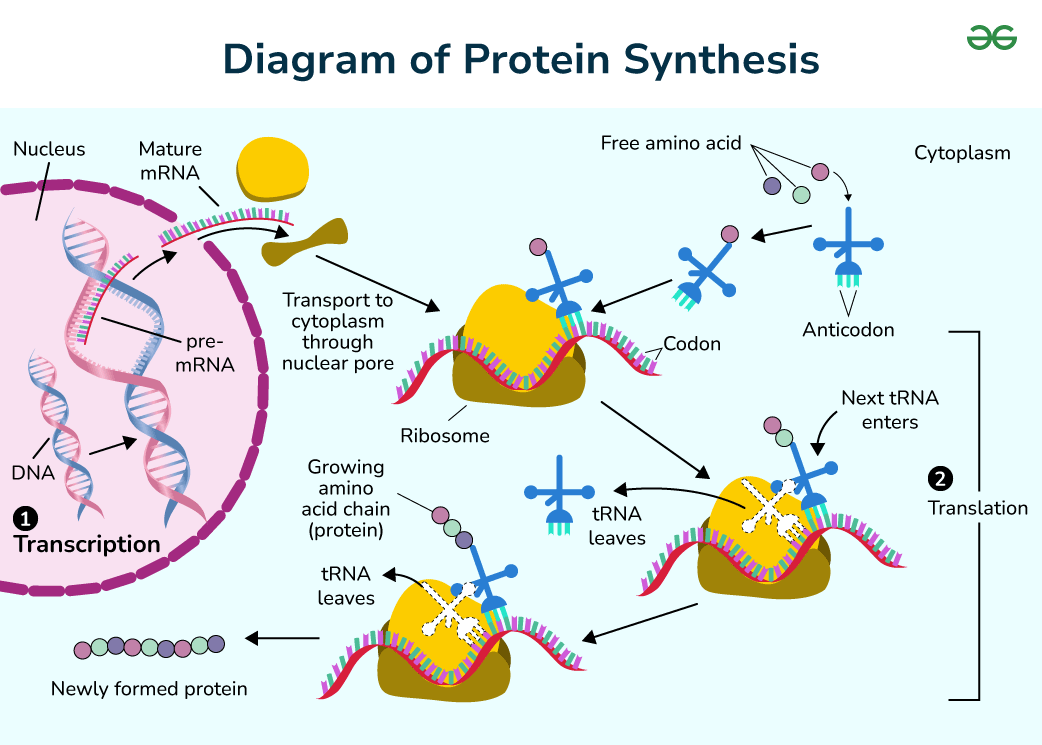
\includegraphics[width=0.9\textwidth]{resources/images/protein_synthesis.png} \\
       \caption{An illustration of the gene translation process in a cell via protein-factories known as ribosomes, and which was sourced from \cite{geeksforgeeks2024protein}}
      \label{FIG2}
    \end{figure} \\
    \cline{1-1} % Bottom border only
  \end{tabular}
\end{table}



    
    
In a later section (\textbf{\hyperref[SEC4]{Chapter \ref{SEC4}}}) we shall deal with [whole] genome expression, and shall especially deal with a particular hypothetical system of genome expression as well as use the modal sequence concept as the basis for exploring expression or manifestation of an entire organism from just its basic genetic code. In this section though, we shall focus on actual expression in real and natural biological systems, and shall focus more on expression at a molecular level --- essentially, at the level of protein manifestation via \textbf{gene expression}.\\


\fbox{\begin{minipage}{0.9\textwidth}
\large

\begin{defn}[The \textbf{DNA and RNA Codon Symbol Sets}, $\psi_{DNA}^*$ and $\psi_{RNA}^*$]
\label{DEFNDNACODONSS}
If $\Theta_n$ is a DNA sequence of length $n$ --- meaning, it contains $n$ nucleotides or $n$ symbols from $\psi_{DNA}$, then, if each triplet of symbols in $\Theta_n$ is replaced by its corresponding 3-gram/CODON, then, we can re-write $\Theta_n$ as a sequence of terms from a special symbol set $\psi_{DNA}^*$:

\begin{equation}
\label{EQSSDNACoDONS}
\psi_{DNA}^* = \langle \alpha_1, \alpha_2, \cdots , \alpha_{64} \rangle
\end{equation}

Such that:

\begin{equation}
\label{EQDNACODCARD}
 \invpi(\psi_{DNA}^*) = \invpi(\psi_{DNA})^3 = 4^3 = 64
\end{equation}

And that each distinct codon has a corresponding standard name associated with either its corresponding amino-acid or whether it is a STOP-codon\cite{gregory1987oxford}\cite{wikipedia_codon_tables}. We shall refer to $\psi_{DNA}^*$ as the \textbf{DNA Codon Symbol Set}.


Further, since RNA sequences are similar to DNA sequences with just the symbols `T' swapped with `U' (see \textbf{\hyperref[DEFRNASS]{Definition \ref{DEFRNASS}}} and \textbf{\hyperref[TRANSF1]{Transformer \ref{TRANSF1}}}), we can also expect that for RNA sequences, there would be an equivalent symbol set for RNA-codons as such:

\begin{equation}
\label{EQSSRNACoDONS}
\psi_{RNA}^* = \langle \beta_1, \beta_2, \cdots , \beta_{64} \rangle
\end{equation}

And the names of the codons in $\psi_{RNA}^*$ are similar to those in $\psi_{DNA}^*$ by the following rule:

\begin{equation}
\label{EQNAMINGRNACodons}
name(\beta_i) = name(\alpha_i) \quad \forall \beta_i \in \psi_{RNA}^*: \beta_i = O_{mRNA-encode}(\alpha_i)
\end{equation}


\end{defn}
\end{minipage}}
\\


It shall be interesting to note that for genetic code in natural automata (nature-like bio-automata\footnote{My research assistant --- thanks \textbf{Microsoft Copilot}, did bring it to my attention that the term ``bio-automata" is ``usually reserved for models or conceptual representations of biological systems --- especially those designed to simulate behaviors, growth patterns, or decisions-making processes using predefined rules, like in cellular automata or agent-based modeling." And thus, much as I often find it attractive to use the term --- as an umbrella term including actual living organisms which, from the perspective of the computer scientist in me, are still correctly classifiable under the ``biological automata" category in my opinion since they actually operate on some infallible inherent natural programs in their DNA. But, I shall adhere to the advise of my assistant for now.} and generally living things), the most important reason the genetic coding language exists, is so that the body/host-organism system can produce required materials as and when they are needed or demanded for. This for example means producing new or extra body tissue in a still growing organism or in one with any damaged or missing tissue, and essentially, such productions are about the synthesis of particular molecules in the body's system that are basically proteins. The diagram in \textbf{\hyperref[FIG2]{Figure \ref{FIG2}}} is a basic illustration of the process for living organisms --- eukaryotes especially.

For simplicity's sake, we can assume the following summarization of the basic process that fully and correctly breaks down the typical ordeal:

First, we shall assume that given the protein is just a chain of amino-acids, we might as well just think of it as though it were a sequence of some terms, and thus, in keeping with the notation from transformatics, we might just refer to such a protein with our usual typical \textbf{resultant sequence} symbol --- $\Theta^*$.

And so, given that these proteins are actually nearly direct/1-to-1 mappings from the corresponding DNA sub-sequence code of a finite length, we might then refer to the DNA sequence that encodes the instructions for producing $\Theta^*$ with just the basic typical transformatics \textbf{source sequence} symbol: $\Theta$ --- more conveniently, because we wish to also talk of the length of the sequence, we might preferably write the DNA sequence code of length \textbf{n} (meaning for example, \textbf{it contains exactly n DNA-codons}), as $\Theta_n$. So, for example we might more fully express $\Theta_n$ as such:

\begin{equation}
\label{EQ1}
\Theta_n = \langle \alpha_{ij}, \rangle ;
\alpha_{ij} \in \psi_{DNA}^* \quad \forall j \in [1,n],  i \in [1,64] \quad \land \quad n \in \mathbb{N}
\end{equation}\\

\textbf{\hyperref[EQ1]{Equation \ref{EQ1}}} being just a sometimes preferable way to write the same exact sequence as:
 
 
 \begin{equation}
\label{EQ2}
\Theta_n = \langle a_1,a_2,a_3,...,a_i,...,a_{n-1},a_n \rangle ;
\forall i \quad \exists a_i \in \psi_{DNA}^* \quad \land \quad n \in \mathbb{N}
\end{equation}\\

We have defined the special symbol sets $\psi_{DNA}^*$ in \textbf{\hyperref[DEFNDNACODONSS]{Definition \ref{DEFNDNACODONSS}}} and  $\psi_{DNA}$ in \textbf{\hyperref[DEFDNASS]{Definition \ref{DEFDNASS}}}, and as for $\psi_{DNA}^*$, we of course know that it essentially is the set of the distinct 64 codons (see \textbf{Table 1} in \cite{gregory1987oxford}) that \textit{especially} encode amino acids, and which were first introduced in \textbf{\hyperref[SEC1]{Chapter \ref{SEC1}}}. Another way to expound on this is by saying that:

 \begin{equation}
\label{EQ3}
\Theta_n = \{a_i \quad | \quad a_i = \prod\limits_{\rho \in \psi_{DNA}}^3 \rho \quad \land \quad \forall i \in [1,n], n \in \mathbb{N} \quad \land \quad \psi_{DNA} = \langle A, C, G, T \rangle\}
\end{equation}\\

Thus we might encounter a gene such as $\Theta_4$ composed of exactly 4 codons as shown below:

 \begin{equation}
\label{EQ4}
\Theta_4 = \langle \langle A, T, G \rangle, \langle A, A, A \rangle, \langle T, T, A \rangle, \langle T, A, G \rangle \rangle
\end{equation}\\

Which, might also equivalently be expressed as a flattened sequence if the fact that the nucleobases it contains are always read in triplets/3-grams/tuples of 3 at a time. So that we can merely write it as:\\

 \begin{equation}
\label{EQ5}
\Theta_{4 \times 3} = \langle  A, T, G, A, A, A, T, T, A, T, A, G \rangle
\end{equation}\\

So we imply that under the flat-structure notation, the sequence has exactly $4 \times 3$ elements. By this fact and the observation that the previous nested notation merely helps to group together each codon's members within a meaningful sub-sequence, and that the order is otherwise maintained in the flat-sequence structure, we might then also equivalently express the same actual DNA code sequence as an $n \times 3$ matrix as shown below:

 \begin{equation}
\label{EQ5a}
\Theta_{4 \times 3} = \begin{pmatrix}
A& T& G\\
A& A& A\\
T& T& A\\
T& A & G \\
\end{pmatrix}
\end{equation}\\


Whether to actually express it as a $3 \times n$ matrix or as $n \times 3$ might be up to the particular taste of the mathematician or scientist, but otherwise, we know that the sequence $\Theta$ in any of the forms above is essentially a \textbf{gene program}\footnote{Indeed, it is right, that any legit natural gene program targeting a codon processor can be expressed as a $n \times 3$ matrix.} or a potential segment of one, that could be used to guide a DNA code processor such as a ribosome, to construct a corresponding protein based on the equivalent transcribed mRNA code sequence --- in this case $\Theta_4^*$, which we might express into mRNA code as such:


 \begin{equation}
\label{EQ6}
\Theta_4^* = \langle \langle A, U, G \rangle, \langle A, A, A \rangle, \langle U, U, A \rangle, \langle U, A, G \rangle \rangle
\end{equation}\\

Which is what we would obtain after a necessary \textbf{DNA} $\rightarrow$ \textbf{mRNA} transform attainable via a DNA sequence transformer we might define as such:\\


\begin{transf}[\textbf{DNA to mRNA Encoder}]
\label{TRANSF1}
$\Theta_n \quad \xrightarrow{O_{mRNA-encode}(\cdot)} \quad \Theta^*_n \quad;$\\
$\forall a_i \in \Theta_n = \langle a_i,\rangle:n \in \mathbb{N}, \quad a_i \in \psi_{DNA} \equiv \{A, T, C, G\}$,\\
and if $\exists a_i \in \Theta_n : a_i = T \implies \exists a_i^* \in \Theta^*_n: a_i^* = U$\\
Otherwise $a_i = a_i^* \implies \invpi(a_i = T \in \Theta_n) = \invpi(U \in \Theta^*_n) \quad \land \quad \invpi(\Theta_n) = \invpi(\Theta^*_n) = n$.

\end{transf}

\begin{table}[h]
  \centering
  \Large
	\begin{tabular}[t]{|c|c|c|p{3cm}|}
	\hline
	i & $a_i$ & \textbf{Amino Acid (Code-name)} & \textbf{Function}\\
	\hline
	\hline
	1 & ATG & Methionine (Met) & Start Codon: initiates translation\\
	\hline
	2 & AAA & Lysine (Lys) & Basic amino acid\\
	\hline
	3 & TTA & Leucine (Leu) & Non polar amino acid\\
	\hline
	4 & TAG & Stop (Amber) & Terminates translation\\
	
	\hline
	              
\end{tabular}
 \caption{Amino-Acid Codes and Names in $\Theta_4$, a DNA-encoded gene}
  \label{TAB1}
\end{table}

Thus, though the gene in its DNA form comprised of the sequence of amino-acid codes named as in \textbf{\hyperref[TAB1]{Table \ref{TAB1}}}, and yet, the resultant sequence after applying \textbf{\hyperref[TRANSF1]{Transformer \ref{TRANSF1}}} to $\Theta_4$ would be as explained in \textbf{\hyperref[TAB2]{Table \ref{TAB2}}}.


\begin{table}[h]
  \centering
  \Large
	\begin{tabular}[t]{|c|c|c|p{3cm}|}
	\hline
	i & $a_i$ & \textbf{Amino Acid (Code-name)} & \textbf{Function}\\
	\hline
	\hline
	1 & AUG & Methionine (Met) & Start Codon: initiates translation\\
	\hline
	2 & AAA & Lysine (Lys) & Basic amino acid\\
	\hline
	3 & UUA & Leucine (Leu) & Non polar amino acid\\
	\hline
	4 & UAG & Stop (Amber) & Terminates translation\\
	
	\hline
	              
\end{tabular}
 \caption{Amino-Acid Codes and Names in $\Theta_4^*$, a mRNA encoded gene}
  \label{TAB2}
\end{table}

So, note that the names (and code-names) of the mRNA encoded codons stay the same as those of their corresponding DNA-encoded codons in both tables --- this is actually generally/conventionally so. But also, note that the functions of the individual codons in either scenario are likewise expressed the same. So, this is because, when the genetic code is actually being executed (such as in standard protein-synthesis\footnote{\textbf{NOTE} that, in reality, protein synthesis is just the tip-of-the-iceberg for what DNA is actually useful for. \textbf{\hyperref[APPOTHERFUNC]{Chapter  \ref{APPOTHERFUNC}}} in the appendix of this book does cover, in summary, 6 other major functions of DNA in a biological system that the reader might wish to be aware of.}), the processor (the ribosome) merely operates on the mRNA-encoded gene and not directly on the original DNA-encoded code sequences.

Also, important to note, the processor only produces an amino acid (as part of the protein synthesis program), only after having encountered a ``start" instruction, and we know that such instructions are the kind encoded by \textbf{start codons}, of which the most universally utilized START-codon is \textbf{ATG/AUG} known as Methionine, but also other rare-scenario\footnote{They are used less frequently, mostly in prokaryotes and some organelles. When used as START codons, they still recruit the initiator tRNA and translate as \textbf{methionine}, not their usual amino acid\cite{copilot_dna_assistant}} START-codons include the mRNA codes GUG and UUG --- used as such in prokaryotes, and then AUU and AUA, used as such in humans only. 

And then, the processor will stop the protein construction task once it encounters a gene instruction of the ``stop" kind. These are encoded using the \textbf{stop codons}, and these are strictly any one of: TAA/UAA (Ochre), TAG/UAG (Amber) and TGA/UGA (Opal)\cite{newsmedical2025startcodons}.

That said, further note that, after processing the gene, and after encountering a stop-codon, the ribosome (also understood as the ``protein factory") is then triggered to detach (from the ``assembly line") and then release/return the final assembled protein thus far. These resultant proteins are basically just a chain of \textbf{actual amino acids} generally starting with the Met-amino acid.

And then, further note that, in case any codons were encountered before the AUG (or rather \textit{start-codon}), these shall then be merely skipped --- they are not processed or would not translate into any product such as the usual case of producing an amino-acid (this, even if they would normally have triggered the production of some amino acid). 

\section{Protein Manufacturing Algorithm}
\label{SECPROT}

So, overall, we might sum up this critically important protein generation process with a convenient formalism such as with a protein-production algorithm expressed as in the flow-chart depicted in \textbf{\hyperref[FIG3]{Figure \ref{FIG3}}}.


\begin{figure}[H]
  \begin{center}
  %\includegraphics[trim=2cm 8cm 2cm 8cm, clip, width=0.9\textwidth,]{resources/pdfs/ProteinSynthesisStateMachine.pdf}\\
   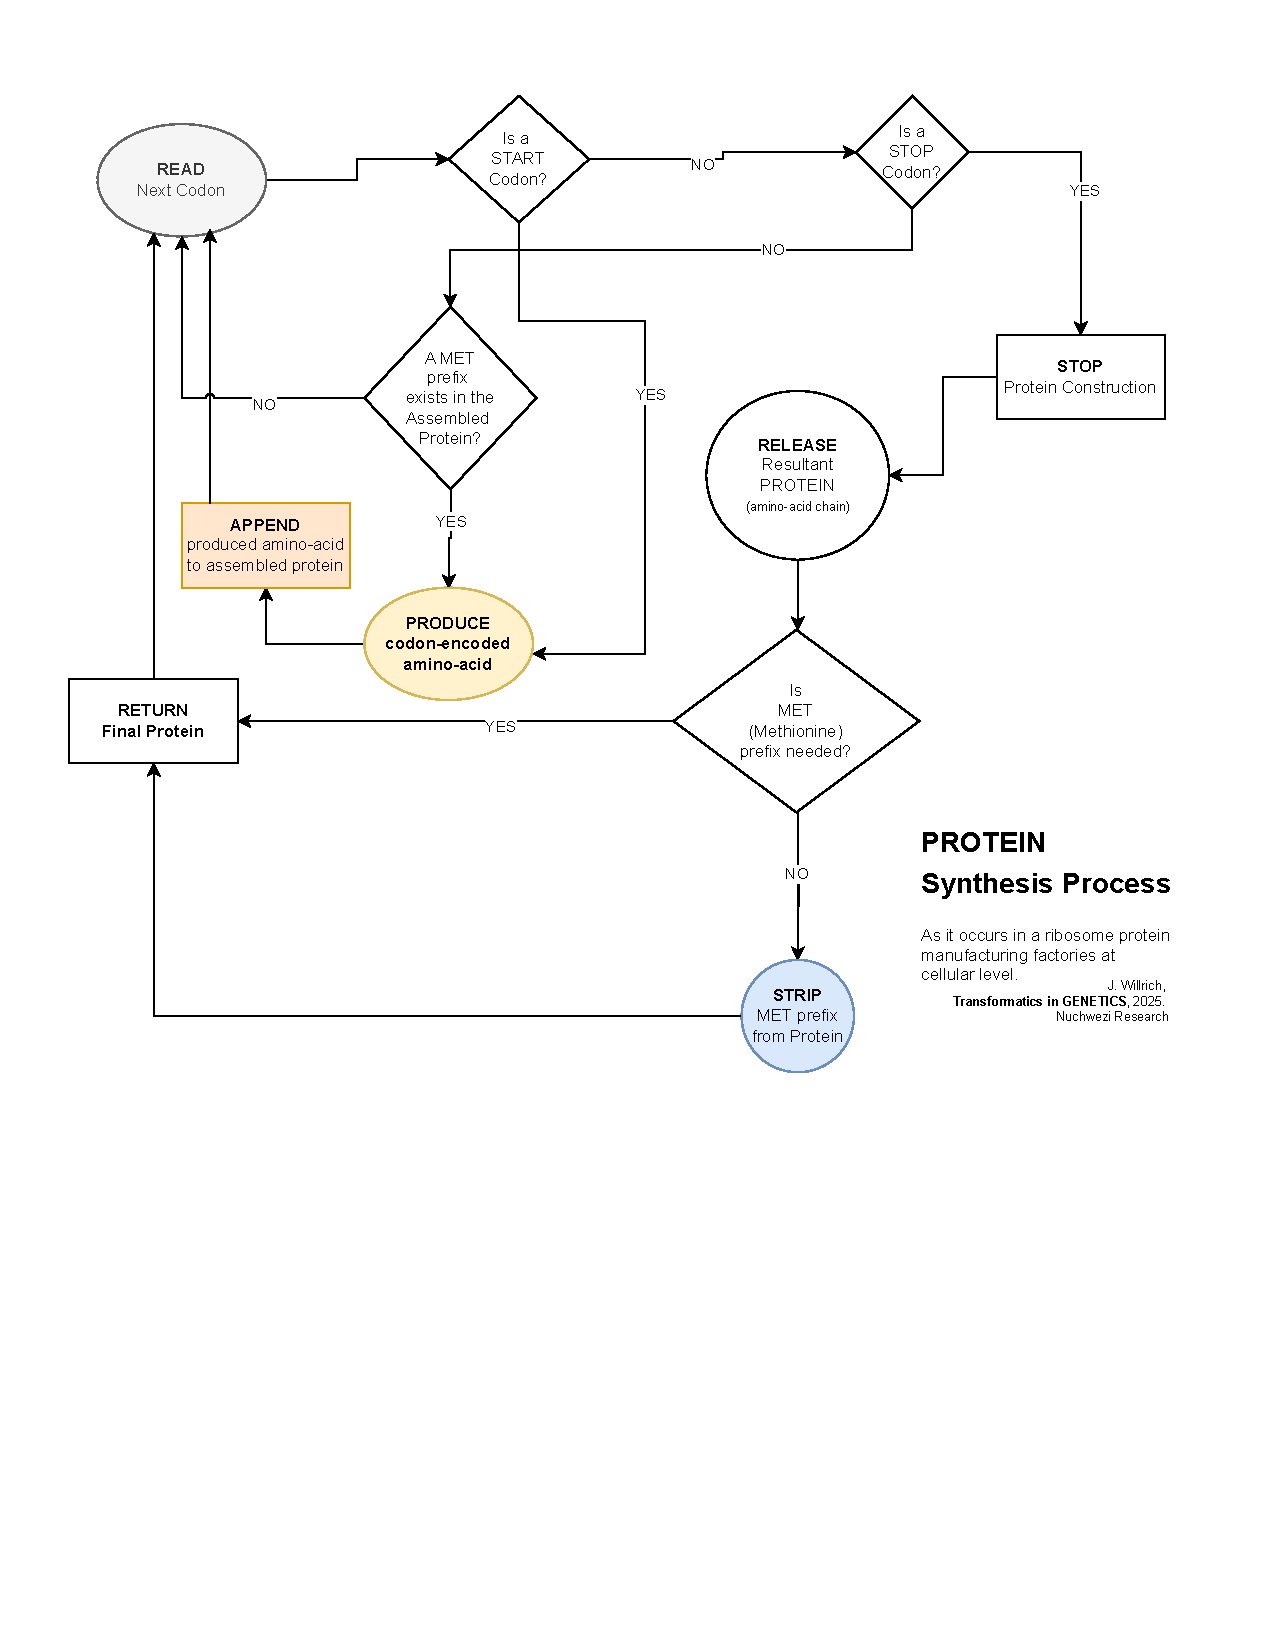
\includegraphics[trim=0cm 8cm 0cm 0cm, clip, width=0.9\textwidth,]{resources/pdfs/ProteinSynthesisProcessFlowChart.pdf}\\
   \caption{\textbf{Flow-Chart summarizing the Ribosome-based Protein-Synthesis Process in a Living Cell}}
  \label{FIG3}
  \end{center}
\end{figure}

That process which is depicted in \textbf{\hyperref[FIG3]{Figure \ref{FIG3}}} is how the ribosome protein-manufacturing\index{ribosome!flow-chart} factory operates at a cellular level as depicted using a \textbf{Flow Chart Diagram} --- meaning, the states of the operating environment as well as those of the operator (the ribosome) are interlaced with decision-making scenarios so as to bring to mind the logic behind how the process proceeds. However, in a different diagram --- the \textbf{Ribosome State Machine} as depicted in \textbf{\hyperref[FIG4]{Figure \ref{FIG4}}}, we clearly abstract everything else away and focus on what actually happens from the point-of-view of the gene code sequence processor --- the ribosome it self. 


In a way, that state machine not only depicts the various states the ribosome shall be in while operating on incoming gene-code sequences (kind of \textit{requests for solutions/solution-instances/proteins} to problems/specifications/genes) and then how it goes about producing the out-going amino-acid sequences (the proteins). It might even start to feel like the ribosome is a kind of 3D-printer, which, when presented with the specifications of a particular 3D-specification-sequence, knows to process it (translate it) and then produce the required/specified [3D-]object that is in the context of biological systems we are looking at here, essentially some protein\footnote{\textbf{FUTURE WORK}: Of course, for someone with a background in computer science and who also has interest in designing not just computer programs but also new kinds of computers --- abstract machines or not, studying the ribosome from a computing theory and computer architecture perspective --- such as; so one appreciates what Instruction Set the ribosome employs; how the ribosome compares to say a Von-Neumann architecture machine; is it Turing Complete or not? How might a pure-text processing languages such as TEA\cite{lutalo2024software} implement a ribosome simulation in say a web-browser environment?\cite{lutalo_tea_web} or that failing at that, at least allow for the creation of a protein generator or even an entire organism generator as a simulation of how gene code sequences can be translated into sequences of multi-dimension objects? etc.}.


\begin{figure}[H]
  \begin{center}
   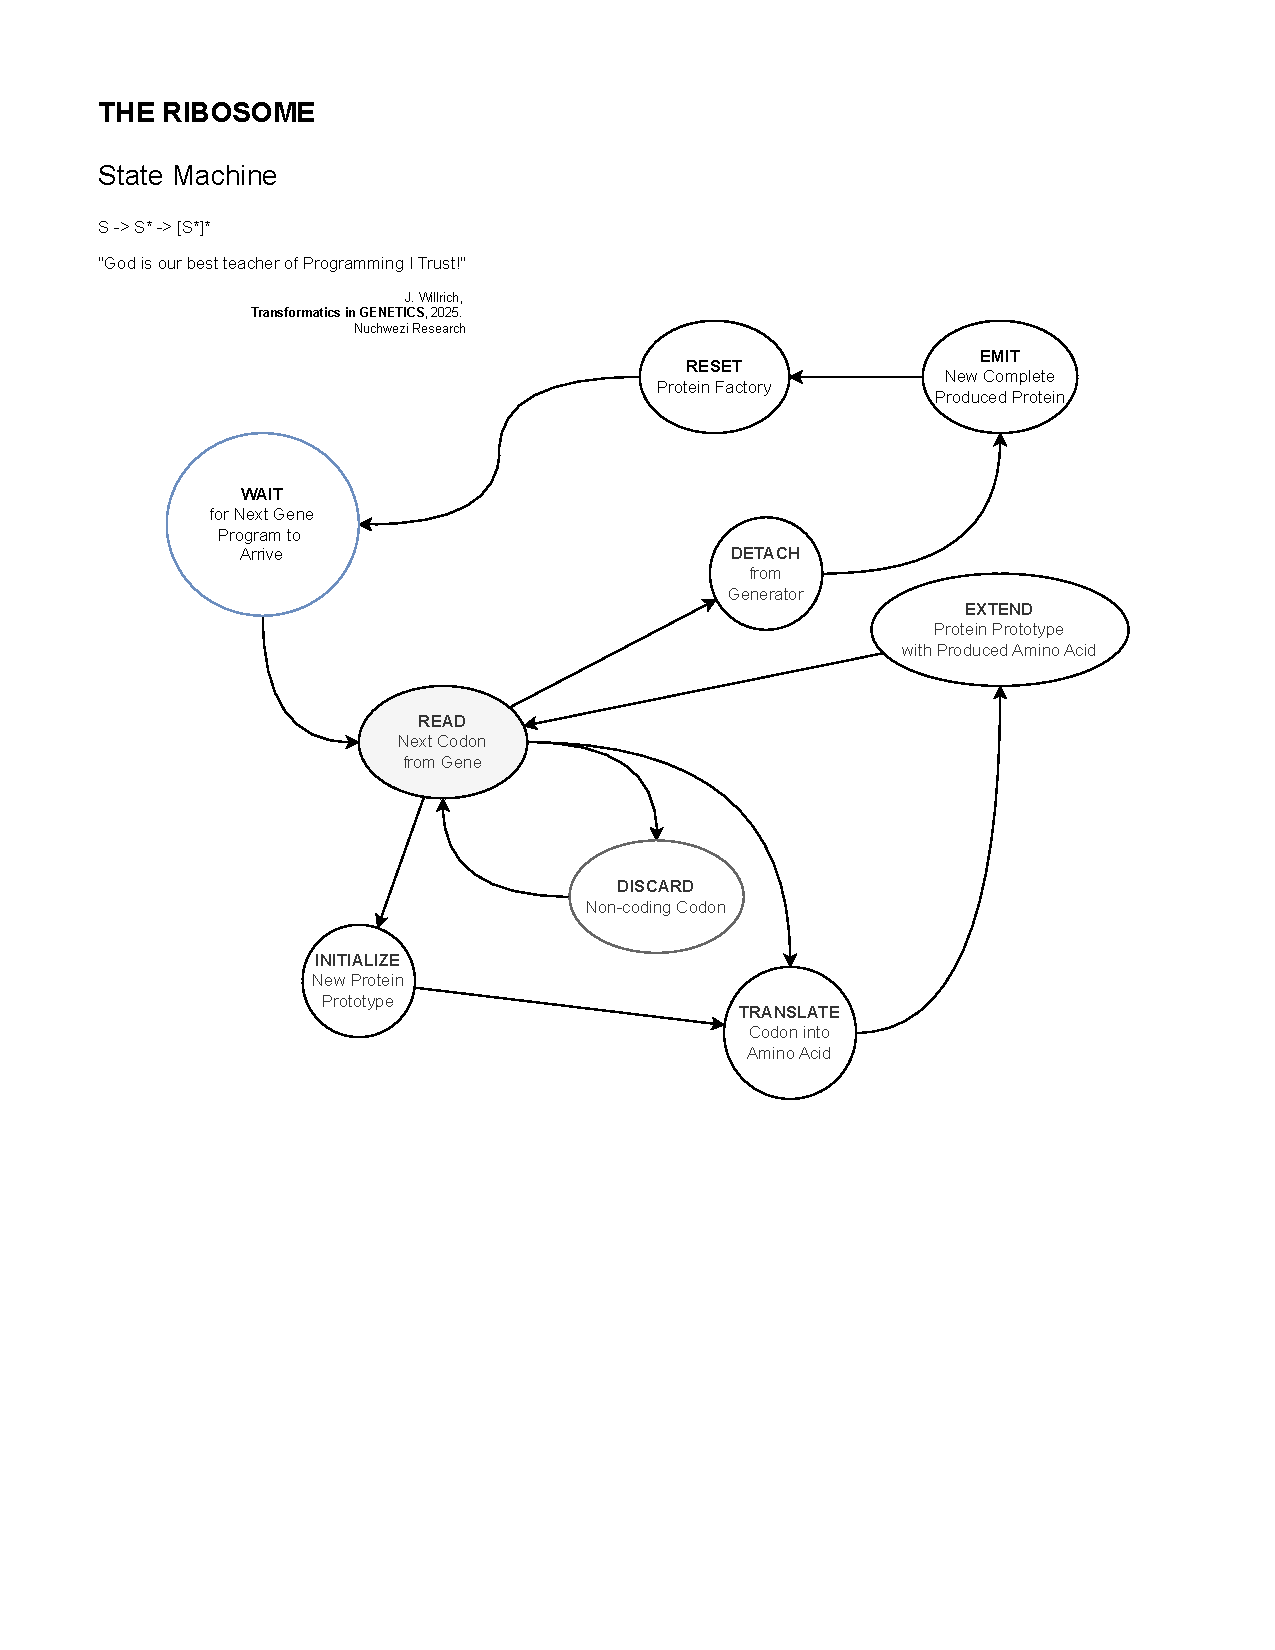
\includegraphics[trim=0cm 9cm 0cm 1.6cm, clip, width=0.9\textwidth,]{resources/pdfs/RibosomeStateMachine.pdf}\\
   \caption{\textbf{The RIBOSOME State Machine}\index{ribosome!state machine}}
  \label{FIG4}
  \end{center}
\end{figure}


Before concluding this section on biological computing systems of the sequence generator kind\cite{lutalo2025transformatic}, it should be worth noting that, as depicted in \textbf{\hyperref[FIG4]{Figure \ref{FIG4}}}, the process that is naturally found in every living thing's tiniest cells (excluding the special case of viruses as we already saw in \textbf{\hyperref[SEC1]{Chapter \ref{SEC1}}}), could be --- as with any legitimate state machine,  used to implement a proof-of-concept [artificial] ribosome processor (or a \textit{ribosome computer}) --- a way to implement bio-automatons that behave like or function like a ribosome; which can process code similar to DNA and mRNA for starters, but also which, generally, operate on sequences to produce other (possibly more complex) sequences. 

Thinking up \textbf{a robotic ribosome} might not be something that is immediately required in contemporary medicine or in-organism computing systems, but might be a concept worth adapting or exploring, for the design and implementation of a self-contained robotic factory for the manufacturing of otherwise complex [multi-form] products producible via use of a sequence-processing, assembly-line kind of method, just like how proteins are produced in a bio-cell by the ribosome, and with the entire process regulated or guided merely using instructions in the form of a sequence [of few symbols from some finite, minimalistic alphabet].

We might for example think of ``a sequence from which a complete, particular type of car can be manufactured at will" or ``a sequence from which certain kinds of sequential-form/sequence-based\footnote{Vertebrates anyone(?)} artificial, but also organic creatures, implements and bots might be systematically assembled at will or on-demand". These kinds of printers --- which, unlike mere printers of \textit{things on paper}, and not just like contemporary 3D-printers that only know to produce plastic variants of models they are fed with, might be the kind of printers with which we might entertain the idea of being able to \textit{print a human}\footnote{\textbf{FUTURE WORK}: Though we might touch on it in a future paper on philosophy --- say one dealing with \textit{Computational Mysticism}\cite{lutalo2024mysticism}, it might be interesting to air-out the author's illuminating view that unlike most other bio-automata such as beasts in the wild or fish in the seas, and definitely not as with silicon-based automatons such as GPT-powered modern \textit{disincarnate} artificial entities --- nor the likes of the ZHA qAGI\cite{jwlzha}, that the human in particular, has this peculiar attribute to them that, apart from just their material substratum as any physical robot might possess or need --- and which is say the domain of ``material producers" such as the ribosome is, and away from their conceptual/software substratum too, they seem to, or perhaps arguably, also possess a preternatural layer of existence that perhaps is or might not have anything to do with their DNA/material-blueprint(?) A better or more precise classification term for such [\textit{preter-}]intelligent -mata/matter(?) might be the still underground term and concept of a \textit{Psymaton} or \textbf{Psymata} --- bits of this line of inquiry have already been touched upon in the Psymaz Interview\cite{lutalo2025unraveling}.}. Such might also be the kind of essential aspects of some machinery with which we might \textbf{teleport}\footnote{Refer to the appendix, \textbf{\hyperref[DEFTELEPORTATION]{Definition \ref{DEFTELEPORTATION}}} for some treatment of this concept.} a cow or a banana, etc. It might be interesting and worth it, to explore, as we look into the far-future, where, with humanity's ability to travel and survive in remote and ``unnatural" worlds away from their biological home environments (such as Earth's biosphere), might compel them to have to develop new kinds of machines that would not only print out ideas on paper, but also be able \textbf{to print complete food ready-to-eat}, medicines to particular kinds of ailments, certain kinds of companion creatures or species, etc. Essentially, the means to survive on/in alien worlds by leveraging smarter, general-purpose sequence processors and generators in form of general-purpose printers. 

Talking of which, the next section shall help us start to appreciate this perspective of using the case of genetic code sequences and the ribosome sequence processor to think of, reason about artificial, conceptual or hypothetical bio-machines that like the bio-cell can produce complex artefacts via the processing of some kind of instruction sequences --- essentially, programmable bio-automata.

\section{Gene Expression in Living Things and for Bio-Automata via Ribosomes}
\label{SEC5}

One might begin by wondering: \textbf{using the concepts from transformatics and pure mathematics, how might we model or express a general and realistic ribosome?} 

A plausible and meaningful solution to this problem would be to begin by acquiring or developing \textit{a rigorous and correct working definition of what a ribosome is.} The answer would follow directly from that, thus our first definition in this section; a formal definition of a ribosome in any system natural or artificial:


%\fbox{\begin{minipage}{0.9\textwidth}

\begin{defn}[A \textbf{Ribosome}]
\label{DEFRIBOSOME}
Assuming we re-write a sequence of DNA code in terms of the [ordered] sequence of nucleotides it contains, as in \textbf{\hyperref[EQ3]{Equation \ref{EQ3}}} re-written as in \textbf{\hyperref[EQ7]{Equation \ref{EQ7}}}:

 \begin{equation}
\label{EQ7}
\Theta_n = \{a_i \quad | \quad a_i = \prod\limits_{\rho \in \psi_{DNA}}^3 \rho \quad \land \quad n \in \mathbb{N} \}
\end{equation}\\

$\Theta_n$ would then be any sequence of DNA-codons of length $n$, equivalent to a flat-structure  sequence of nucleotides of length $n \times 3$. We can then produce mRNA-codons from $\Theta_n$ as per \textbf{\hyperref[TRANSF1]{Transformer \ref{TRANSF1}}}, so that we produce a new mRNA-codon sequence of length $n$ that is generated as such:

\begin{trans}
\label{TRANS1}
$\Theta_n \quad \xrightarrow{O_{mRNA-encode}(\cdot)} \quad \Theta^*_n;$\\
$\Theta^*_n = \{a_i^* \quad | \quad a_i^* = \prod\limits_{\rho \in \psi_{RNA}}^3 \rho \} \quad \land \quad \invpi(\Theta_n) = \invpi(\Theta^*_n) = n$
\end{trans}

And with $\Theta^*_n$ thus produced, we can then merely generate the corresponding sequence of amino-acids, denoted as $[\Theta^*_n]^*$, via the following mRNA to amino-acid transformer: 

\begin{transf}[\textbf{mRNA to Amino-Acid Translator}]
\label{TRANSF2}
$ $\\
$\Theta^*_n \quad \xrightarrow{O_{mRNA-translate}(\cdot)} \quad [\Theta^*_n]^* \quad;$\\
\begin{enumerate}
\item $\invpi([\Theta^*_n]^*) < \invpi(\Theta^*_n)$ because\footnote{\textbf{FUTURE WORK}: Verify, either empirically or theoretically, whether indeed this inequality is universally true or whether there is a computable upper limit to the length of the produced amino-acid sequence relative to the length of the gene program sequence that describes its production.} we only count each codon in the source once, and as per the rules of gene processing/transcription, all non-coding codons (introns) --- basically, codons not able to be translated into an amino-acid given the state of the gene processor\footnote{See \textbf{\hyperref[FIG3]{Figure \ref{FIG3}}} and \textbf{\hyperref[FIG4]{Figure \ref{FIG4}}}} don't contribute to the generated resultant sequence in terms of sections it contains --- with the exception of the special ``Met" codon\footnote{A START-codon also counted among genuine ``exons" --- coding codons.} that might or might not be retained in the resultant sequence even though it is automatically included as the first produced amino-acid in any legitimate gene sequence transcription result.
\item The entire sequence $[\Theta^*_n]^*$ is a kind of 3-Dimension molecule based on the chain of amino-acids it contains, and is technically referred to as a protein.
\end{enumerate}
$\qed$
\end{transf}

A \textbf{Ribosome} then, is any combination of transformers that can result in $[\Theta^*_n]^*$ when presented with just $\Theta_n$ as per the two intermediate transformer processes \textbf{\hyperref[TRANSF1]{Transformer \ref{TRANSF1}}} and \textbf{\hyperref[TRANSF2]{Transformer \ref{TRANSF2}}}, and whose overall processing algorithm is as depicted in \textbf{\hyperref[FIG3]{Figure \ref{FIG3}}} and its corresponding state machine as in \textbf{\hyperref[FIG4]{Figure \ref{FIG4}}}. 

So, overall, a ribosome is any machine that can implement the combined transformer defined as in \textbf{\hyperref[TRANSF3]{Transformer \ref{TRANSF3}}}:

\vspace{1em}

\begin{transf}[The \textbf{Protein Generator} (A Ribosome)\index{generator!protein generator}\index{ribosome}]
\label{TRANSF3}
$ $\\
$\Theta_n  \xrightarrow{O_{mRNA-encode}(\cdot)}  \Theta^*_n  \xrightarrow{O_{mRNA-translate}(\cdot)} [\Theta^*_n]^*;$\\
$\invpi([\Theta^*_n]^*) < \invpi(\Theta^*_n) = \invpi(\Theta_n) = n:$\\
$\psi_{\Theta} \subseteq \psi_{DNA} \quad \land \psi_{\Theta^*_n} \subseteq \psi_{RNA} \quad \land \psi([\Theta^*_n]^*) \subseteq \psi_{amino-acids}$
\end{transf}

And thus, we can finally merely call any machine capable of implementing the protein generator  in \textbf{\hyperref[TRANSF3]{Transformer \ref{TRANSF3}}} as a \textbf{Ribosome}.

\end{defn}

%\end{minipage}}
%\\




\chapter{Transformatics and Lu-Genome Expression System in Bio-Automata}
\label{SEC4}


\begin{table}[H]
  \centering
  \begin{tabular}{|p{0.95\textwidth}} % Left border only
    \hline
    \begin{figure}[H]
      \centering
      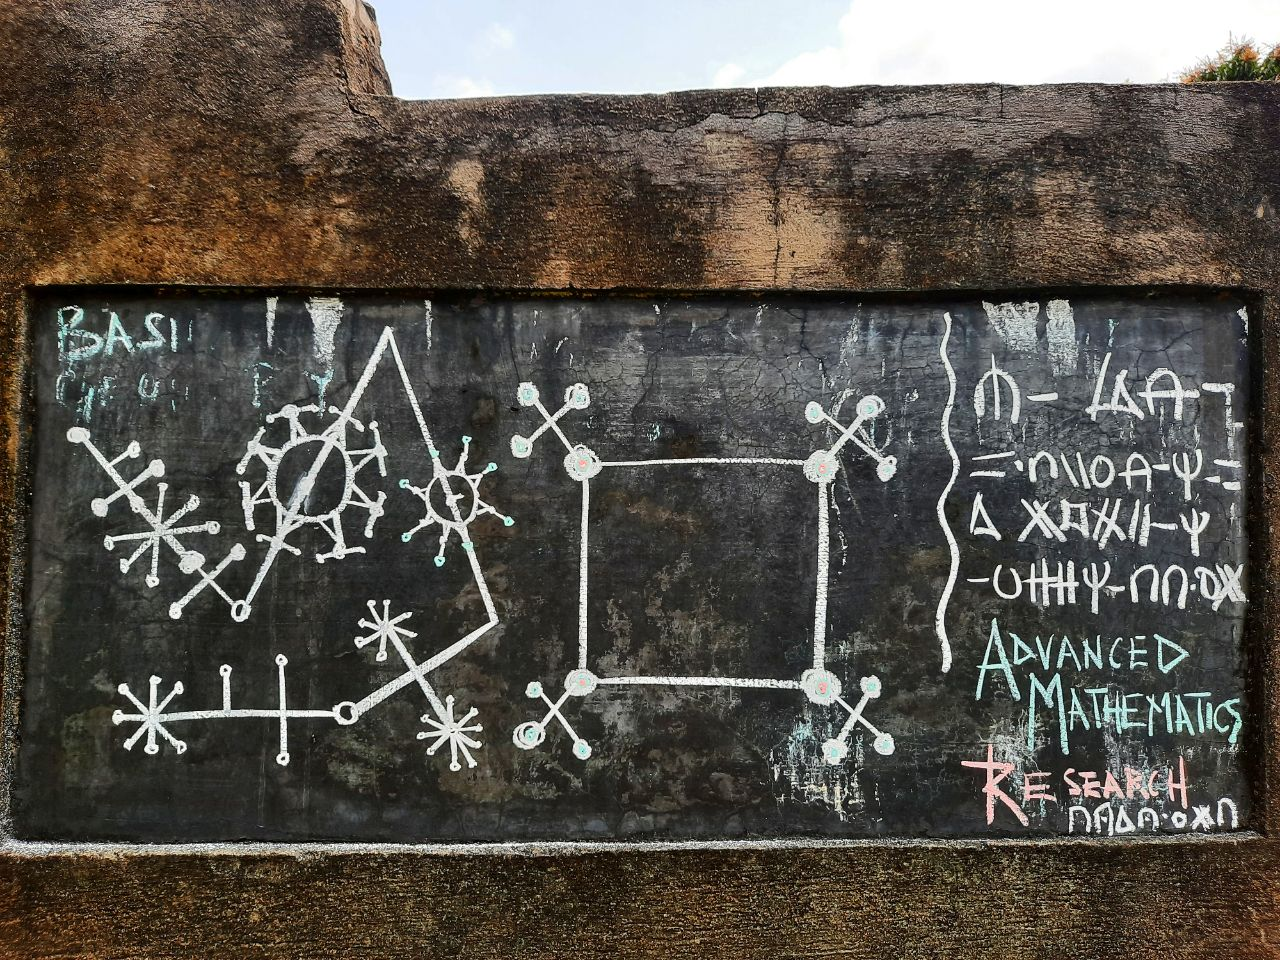
\includegraphics[width=0.9\textwidth]{resources/images/lugenome_expression.jpg}\\
      \caption{A blackboard snapshot from the author's \textbf{Blackboard Adventures} (\url{https://t.me/bclectures}) series on Telegram, on \textbf{20$^{th}$ AUG, 2025}, depicting two \textbf{LGES} example genome expressions, one for $\overset{>}{\Theta} = \langle 218 \rangle$, the other for the \textbf{PFA} segment configuration $4_{pf}\otimes6_{oz}$}.
      \label{FIGBCLECTURE}
    \end{figure} \\
    \cline{1-1} % Bottom border only
  \end{tabular}
\end{table}


\vspace{2em}

\noindent
\begin{minipage}{1\textwidth}
\vspace{1em}
\begin{quotation}
\noindent {\ttfamily

\textbf{Genome Expression}: The collective expression profile of all genes within a genome, including coding and non-coding regions, across different conditions, cell types, or developmental stages. It is a systems-level view - measuring how the entire genome behaves dynamically. This includes: mRNA expression of all genes, noncoding RNA activity, epigenetic regulation, chromatin accessibility and transcriptional networks. In essence, gene expression is local, while genome expression is global.

}
\hspace*{\fill} --- \textbf{Microsoft Copilot}\cite{copilot_dna_assistant}
\end{quotation}
\vspace{1em}
\end{minipage}

\vspace{2em}




We shall use \textbf{a thought experiment} and \textit{hypothetical cases} leveraging \textbf{exemplary} genetic code modeled using special sequences that are treated as \textbf{modal sequences} at minimum.


\vspace{2em}
\fbox{
\begin{minipage}{0.9\textwidth}
\textbf{Applying Transformatics:}\\

Away from using transformatics to make sense of the differences between organisms based on their genetic code sequences, an even more exciting application of the theory and practical methods of transformatics would be in conceptualizing, analyzing and explaining the important, biological, physical, chemical, informational, mathematical, and \textit{aesthetic} concept of \textbf{genome expression}.

\end{minipage}}
\\



\vspace{2em}
First, we shall define a basic cipher that can encode the basic digits (of base-10), as some unique, but non-digit forms (essentially, with non-digit \textit{glyphs}). This, so when we speak of a living organism --- for example a pine-apple or a feline, we don't expect that in nature, or rather, that by physically dissecting the organism, that one shall find trapped or stored inside it, the literal genetic code symbols (such as those in $\psi_{na}$), but rather, that they shall find natural literal expressions or instances of genetic code's \textbf{material basis} --- such as the chemical base molecules that define nucleobases, or nucleotides, and also complex molecular structures such as transcribed amino-acids post-RNA translation of DNA expressions.

So, in our hypothetical genome expression model --- the \textbf{Lu-Genome Expression System} (LGES), we are going to expect and express elements from our basic hypothetical DNA symbol set --- an alphabet\footnote{In our mathematics, and especially in Transformatics, we conventionally talk of \textbf{a symbol set} where other literature might talk of \textit{an alphabet}.} we shall call \textbf{Base-Omega}.\\

\begin{equation}
\label{EQHYPDNASS}
\psi_{\Omega} = \langle 0, 1, 2, 3, 4, 5, 6, 7, 8, 9 \rangle \equiv \psi_{10}
\end{equation}\\

Which, especially for curiosity's sake, but also, for creative and expressive reasons, is meant to allow us to explore a peculiar genetics model based not on just some four base symbols as is the case in $\psi_{DNA}$, but which allows us to look at any base-10 number expression --- essentially any \textit{decimal sequence}\index{sequences!decimal}\index{number expression} --- as a potential genetic code sequence with \textbf{each digit expressing a distinct hypothetical nucleic acid}. 


For example, we might describe some fictitious organism --- for simplicity's sake, perhaps, just a virus, that we shall name \textbf{the Euler Virus}\footnote{I called it that, simply because of the fact the associated genome sequence is based on the important natural physical constant --- 2.718281828459, the \textbf{Euler number}, that is one of those irrational numbers that also happens to be the base of the natural logarithm and which arises naturally in many areas of mathematics, especially in calculus, complex analysis, and probability theory.} or just ``veuler", as having its entire genome sequence encoded as just:

\begin{equation}
\label{EQDNAV}
\Omega_{veuler} = 27182818
\end{equation}


However, that is the DNA-side of the story. As in real nature, we need a \textit{different} alphabet or symbol set for expressing genetic code in its \textit{intermediate form} --- as genome expression typically proceeds via expression of DNA into mRNA first of all, and then finally into functions such as proteins. So, in our case, the intermediate expressions shall be expressed using the \textbf{Ozin Cipher}\footnote{More about this in the \textbf{\hyperref[APPOZIN]{Appendix}}.}, which we are to describe hereafter.


\section{The Ozin Genetic Code Cipher}
\label{SECOZIN}

With the background we have obtained thus far, note that, the special \textbf{transcription level} expression of our genetic code originally expressed via $\psi_{10}$, shall be transcribed into the intermediate \textbf{ozin genetic code} that spans the symbol set $\psi_{oz}$ that is mapped from the genetic code's storage expression, via a mapping as depicted in \textbf{\hyperref[FIGOZIN]{Figure \ref{FIGOZIN}}}.



\begin{figure}[H]
  \begin{center}
  %\includegraphics[trim=2cm 8cm 2cm 8cm, clip, width=0.9\textwidth,]{resources/pdfs/ProteinSynthesisStateMachine.pdf}\\
   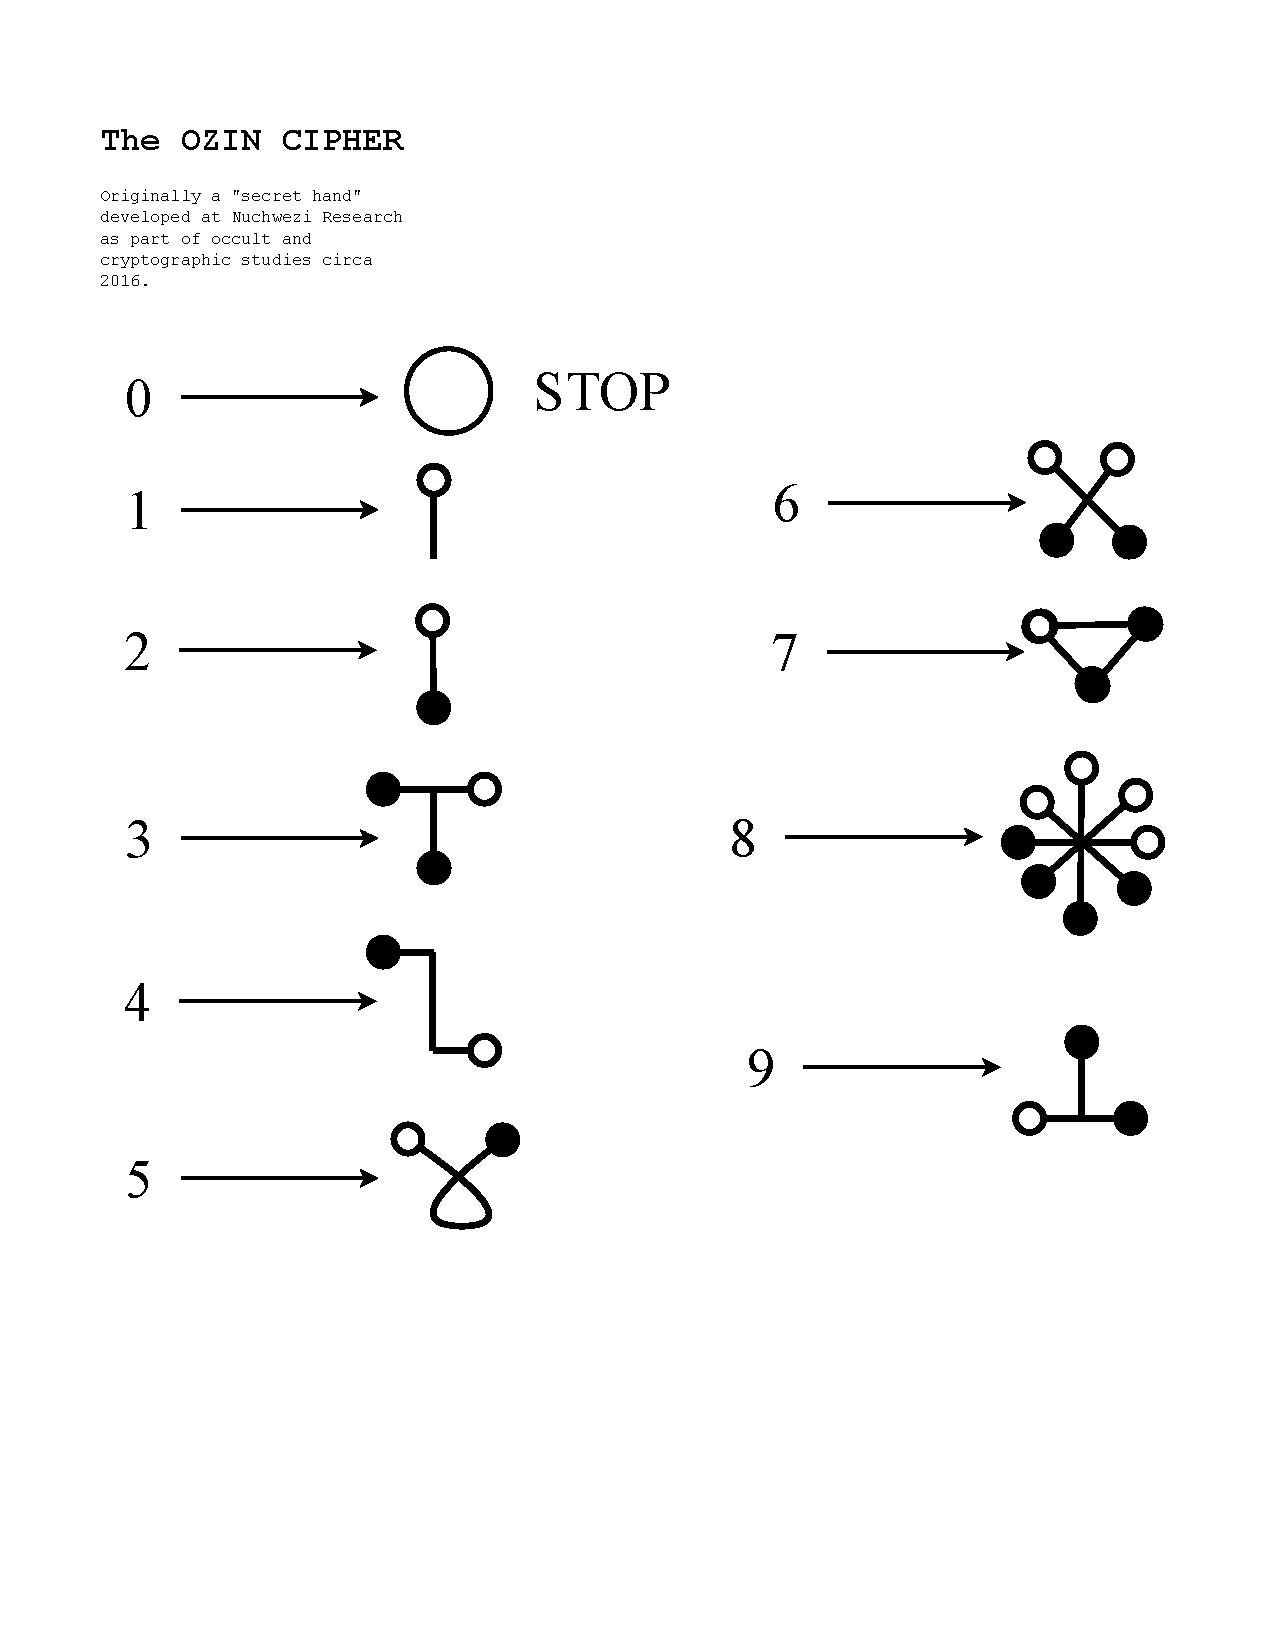
\includegraphics[trim=0cm 6cm 0cm 0cm, clip, width=0.9\textwidth,]{resources/pdfs/OZINCIPHER.pdf}\\
   \caption{The OZIN Cipher\cite{lutalo_2025_ozin}, a mapping from Decimal Symbols (our base-$\Omega$) to Symbols for Intermediate Genetic Code.}
  \label{FIGOZIN}
  \end{center}
\end{figure}


For simplicity's sake, we might interpret or transcribe from base-$\Omega$ DNA into our base-OZ RNA expression as such:

If for some organism such as that expressed via $\Omega_{veuler} = 27182818$, we wish to encode the equivalent intermediate [physical] expression, then we iterate through each symbol in the source code sequence, and re-write it as the equivalent symbolic structure in OZIN, and this, so as to center the ozin glyphs along a \textbf{backbone structure} of just a mere line that starts with a tiny dot and ends with the last ozin structure from the source sequence thus transcribed. Essentially, for our
Euler Virus, it would render as something of the sort shown in \textbf{\hyperref[FIGOZEVIRUS]{Figure \ref{FIGOZEVIRUS}}}

\begin{figure}[H]
  \begin{center}
  %\includegraphics[trim=2cm 8cm 2cm 8cm, clip, width=0.9\textwidth,]{resources/pdfs/ProteinSynthesisStateMachine.pdf}\\
   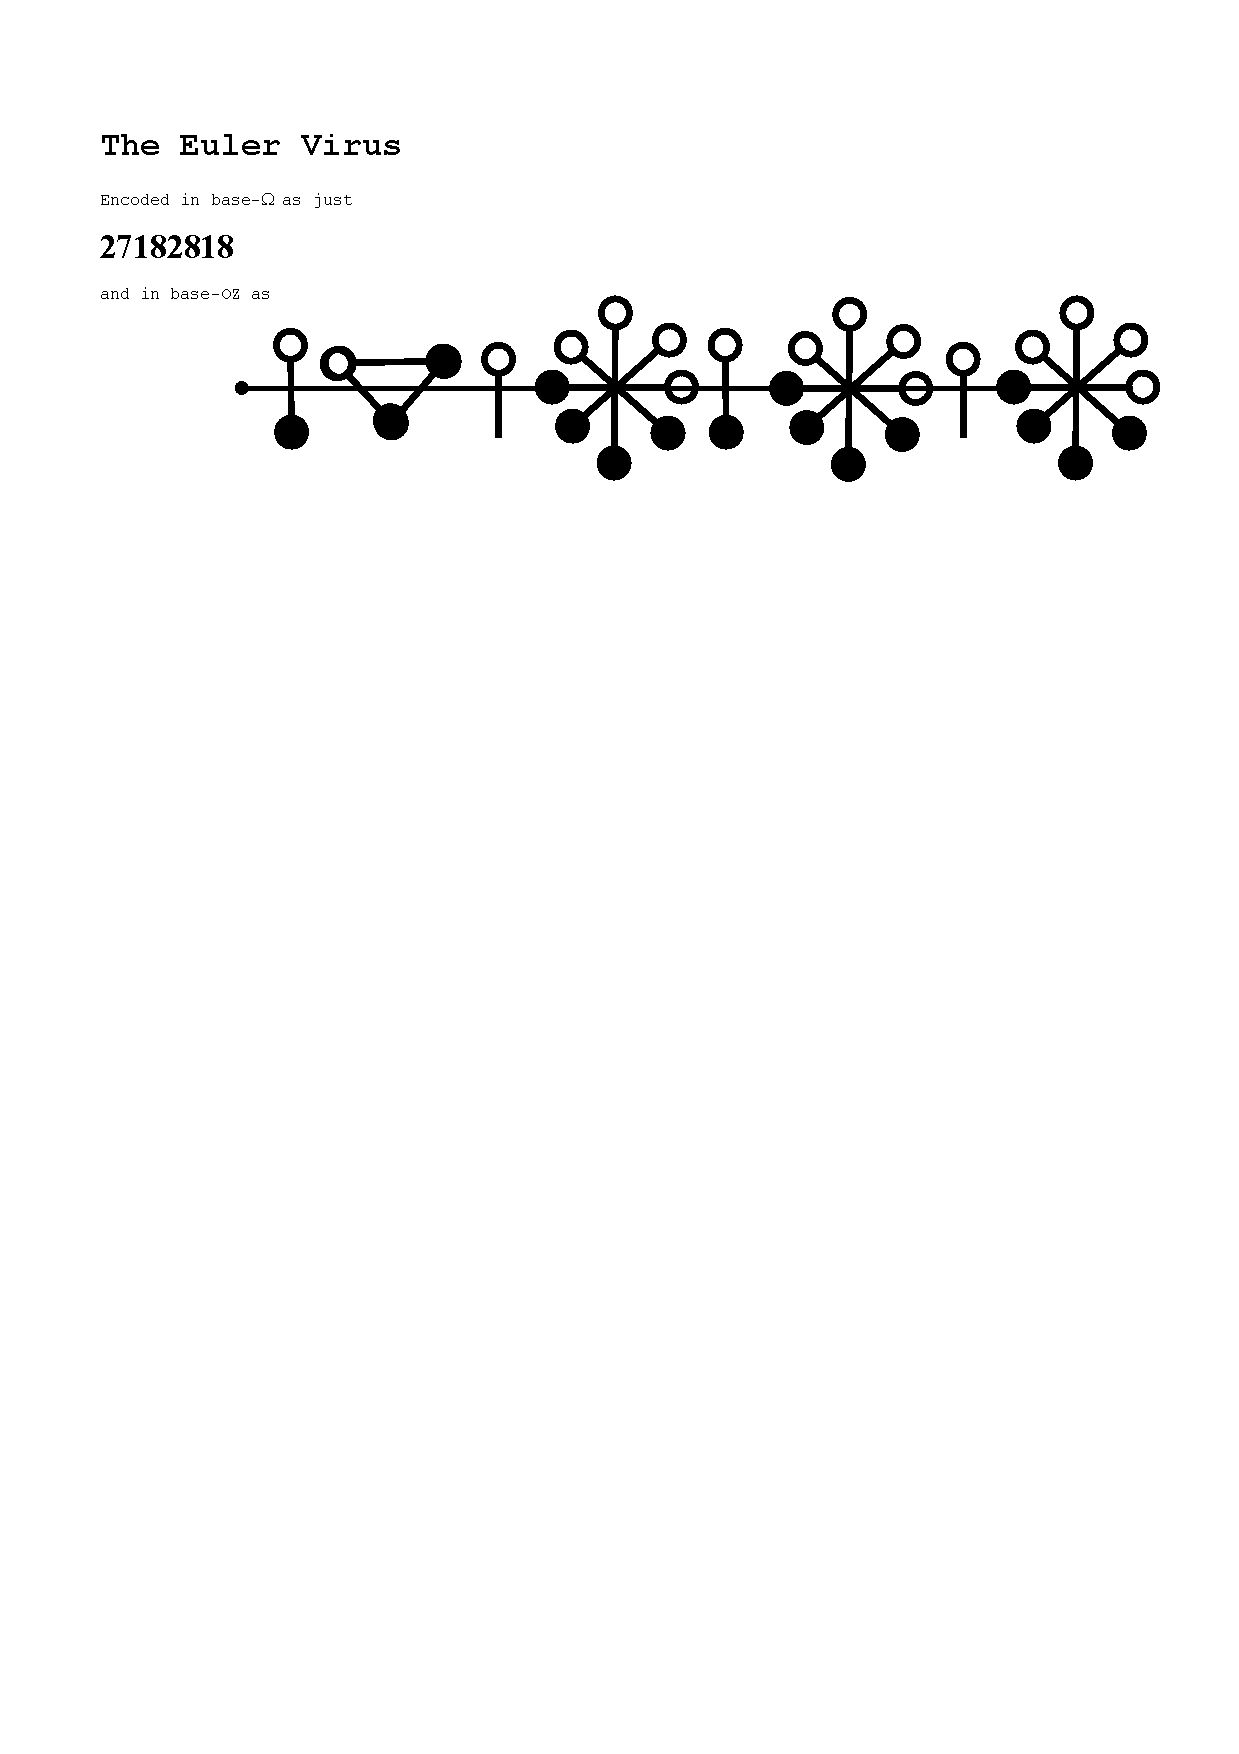
\includegraphics[trim=0cm 20cm 0cm 0cm, clip, width=0.9\textwidth,]{resources/pdfs/OZINCIPHER-APP1-EVIRUS.pdf}\\
   \caption{The equivalent OZIN expression of the hypothetical Euler Virus genome sequence.}
  \label{FIGOZEVIRUS}
  \end{center}
\end{figure}


Another organism, which we might just refer to as the \textbf{HiFinelle}, is actually based off of our favorite base-10 o-SSI --- the \textbf{Hi-Fi o-SSI}\cite{adtpaper}, and thus, its corresponding genetic code at rest is as:


\begin{equation}
\label{EQDNHIFI}
\Omega_{HiFinelle} = 8649137520
\end{equation}


And which, after we have it transcribed into intermediate OZIN genetic expression, shall appear as shown in \textbf{\hyperref[FIGOZHIFI]{Figure \ref{FIGOZHIFI}}}


\begin{figure}[H]
  \begin{center}
  %\includegraphics[trim=2cm 8cm 2cm 8cm, clip, width=0.9\textwidth,]{resources/pdfs/ProteinSynthesisStateMachine.pdf}\\
   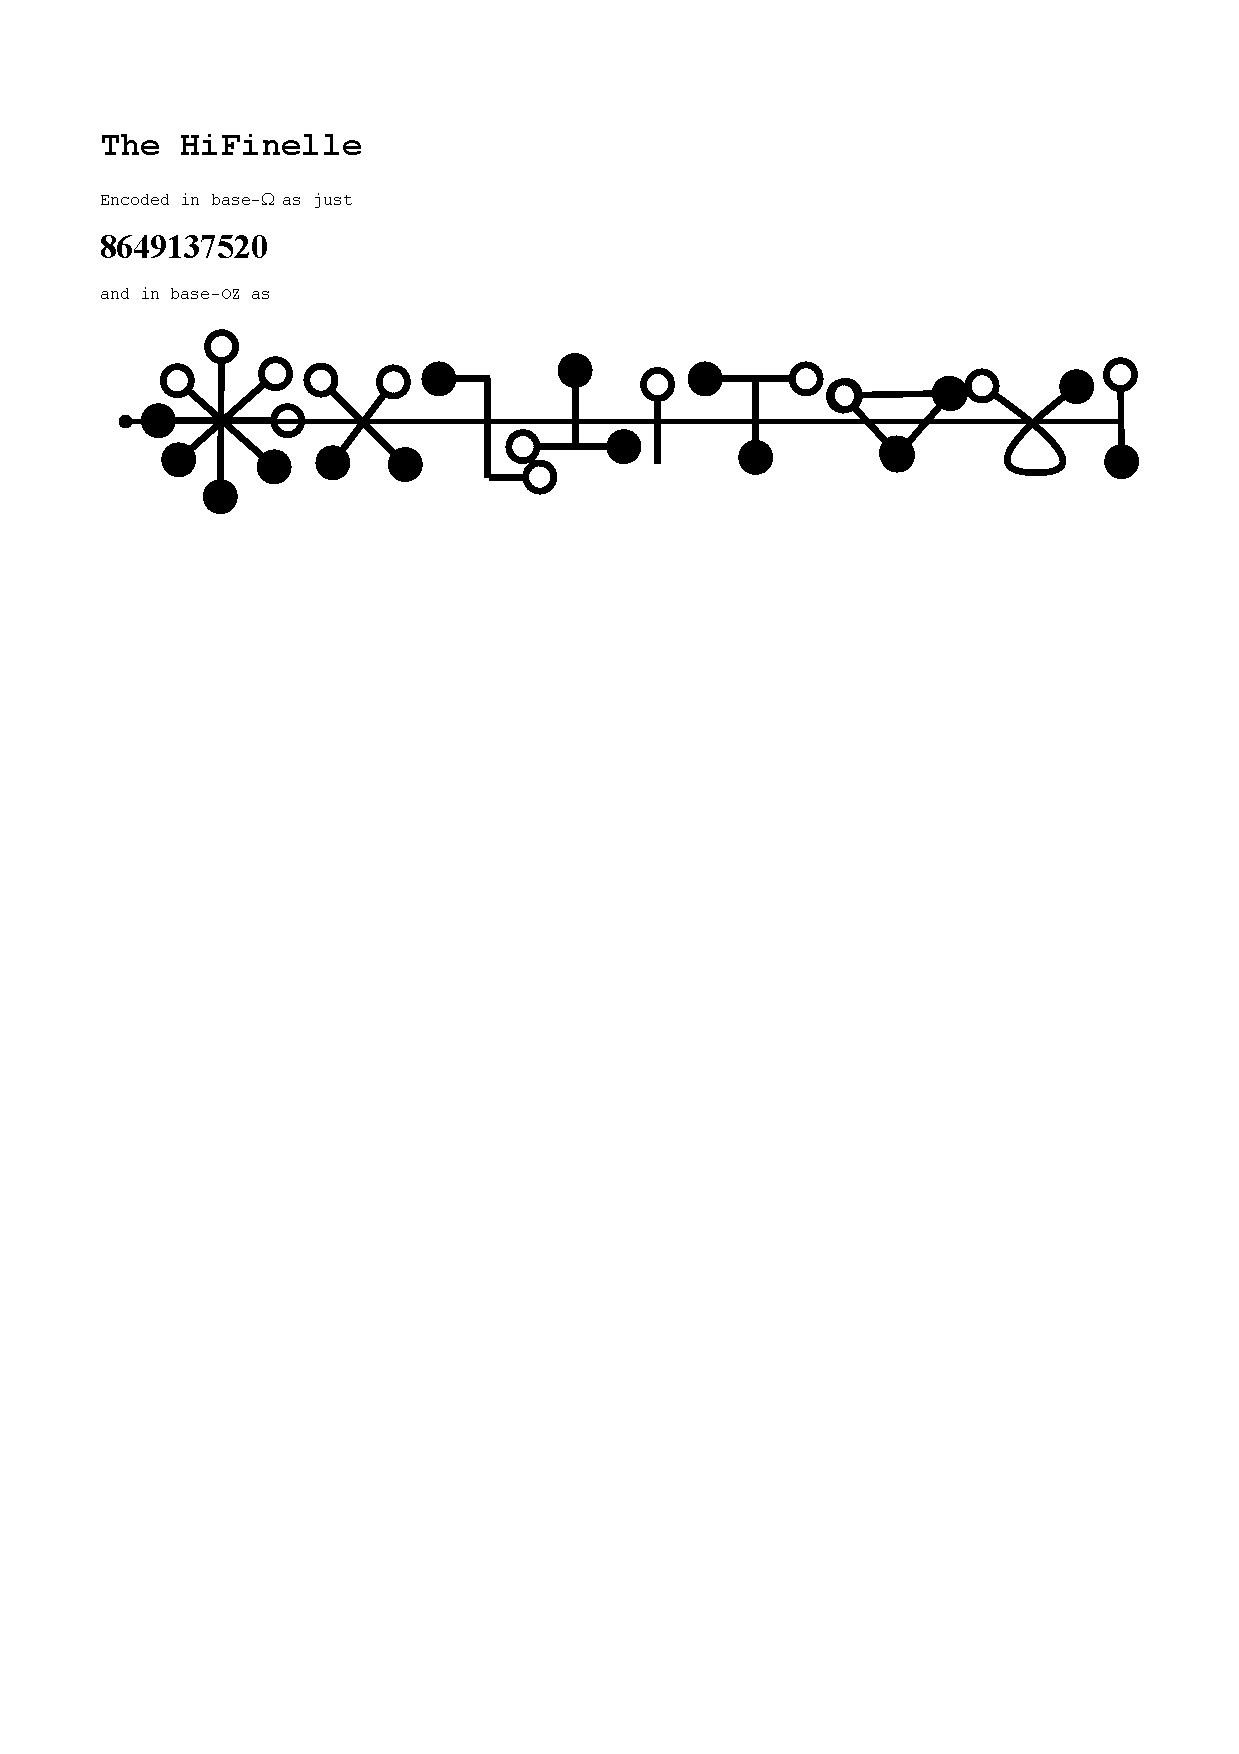
\includegraphics[trim=0cm 20cm 0cm 0cm, clip, width=0.9\textwidth,]{resources/pdfs/OZINCIPHER-APP2-HIFINELLE.pdf}\\
   \caption{The equivalent OZIN expression of the HiFinelle genome sequence.}
  \label{FIGOZHIFI}
  \end{center}
\end{figure}

Of course, in our simple genome expression system, the occurrence of that last ``0" symbol in the HiFinelle genome sequence tells us to STOP or just exclude that symbol with a GAP in case any other symbols follow thereafter. It is our STOP-codon equivalent.

Another genome sequence,\\

\begin{equation}
\label{EQDNEXA}
\Omega_{3} = 0123026
\end{equation}\\

Might help illustrate that point --- see \textbf{\hyperref[FIGOZEXA]{Figure \ref{FIGOZEXA}}}


\begin{figure}[H]
  \begin{center}
  %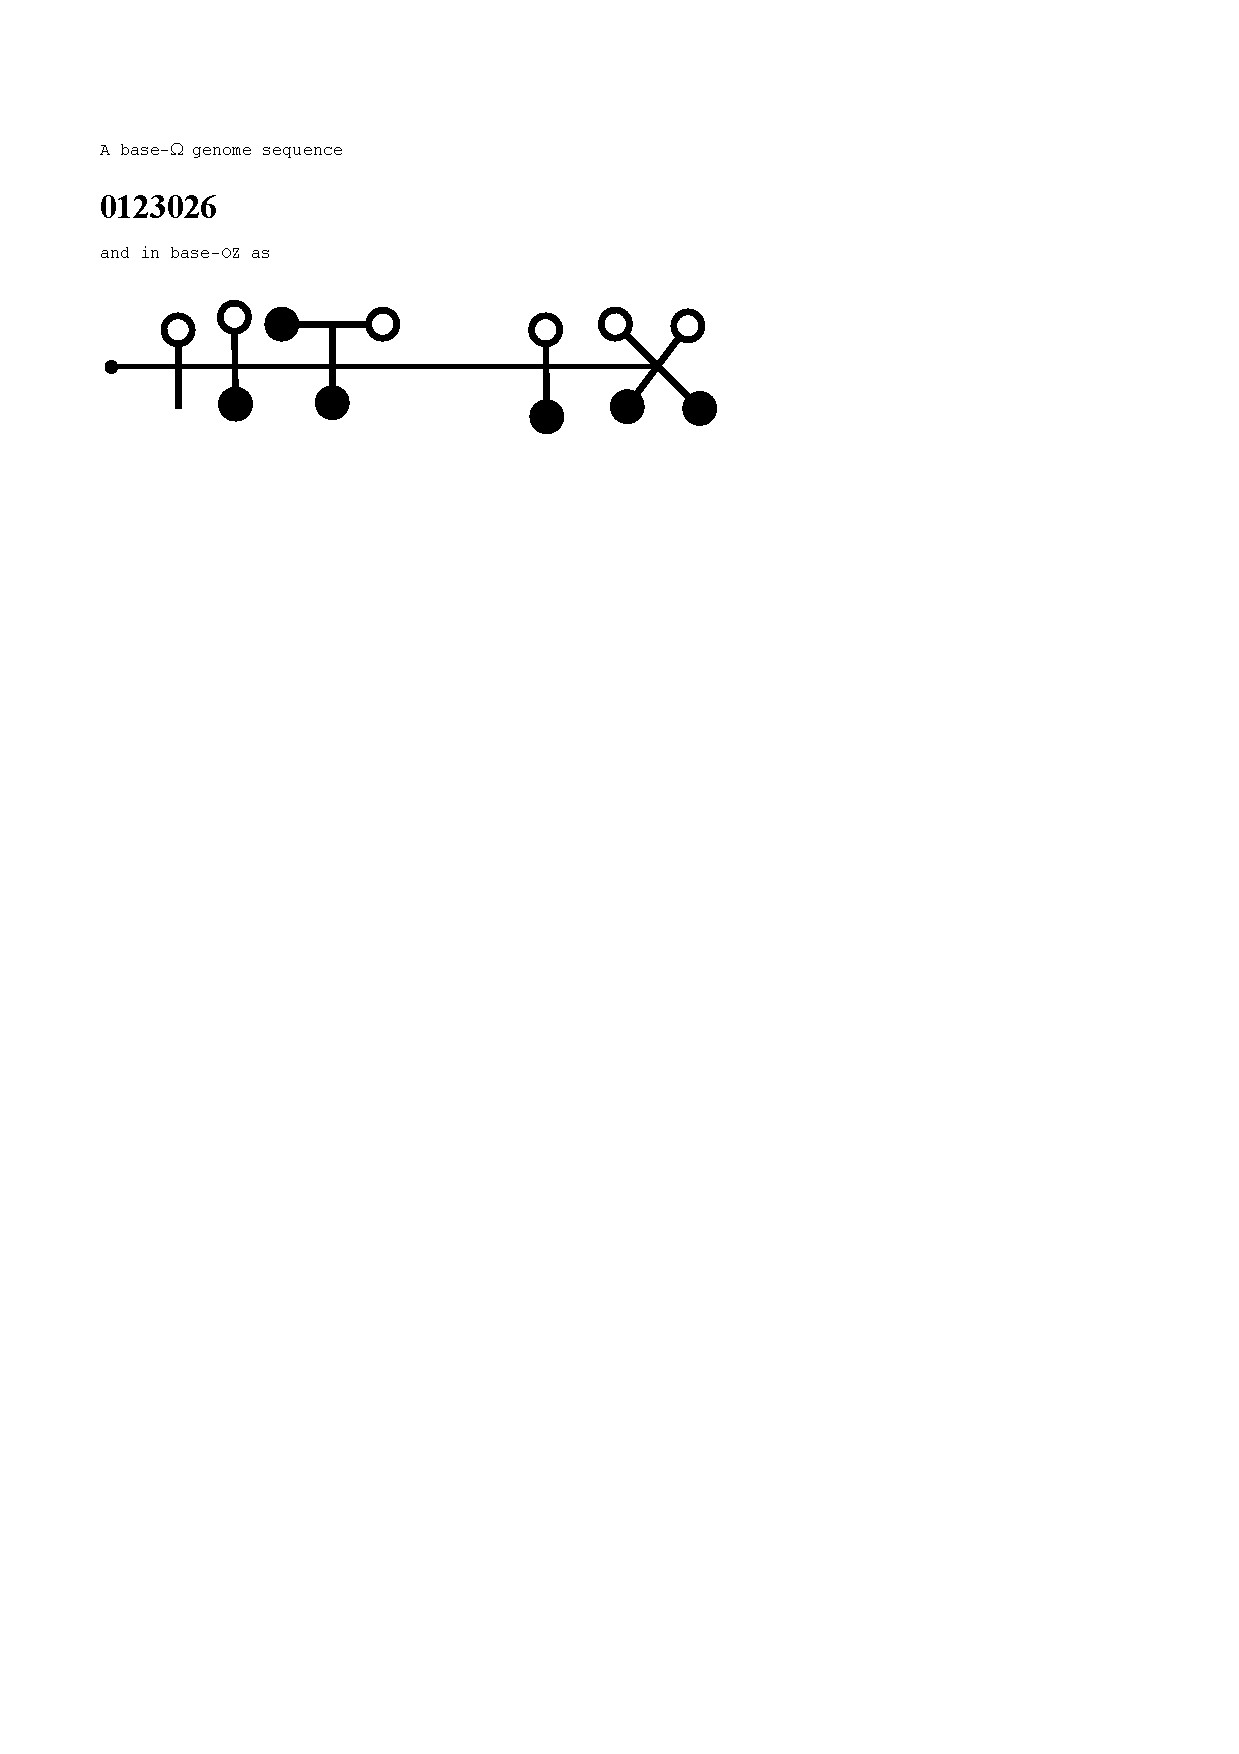
\includegraphics[trim=0cm 20cm 0cm 0cm, clip, width=0.9\textwidth,]{resources/pdfs/OZINCIPHER-APP3-EXA.pdf}\\
   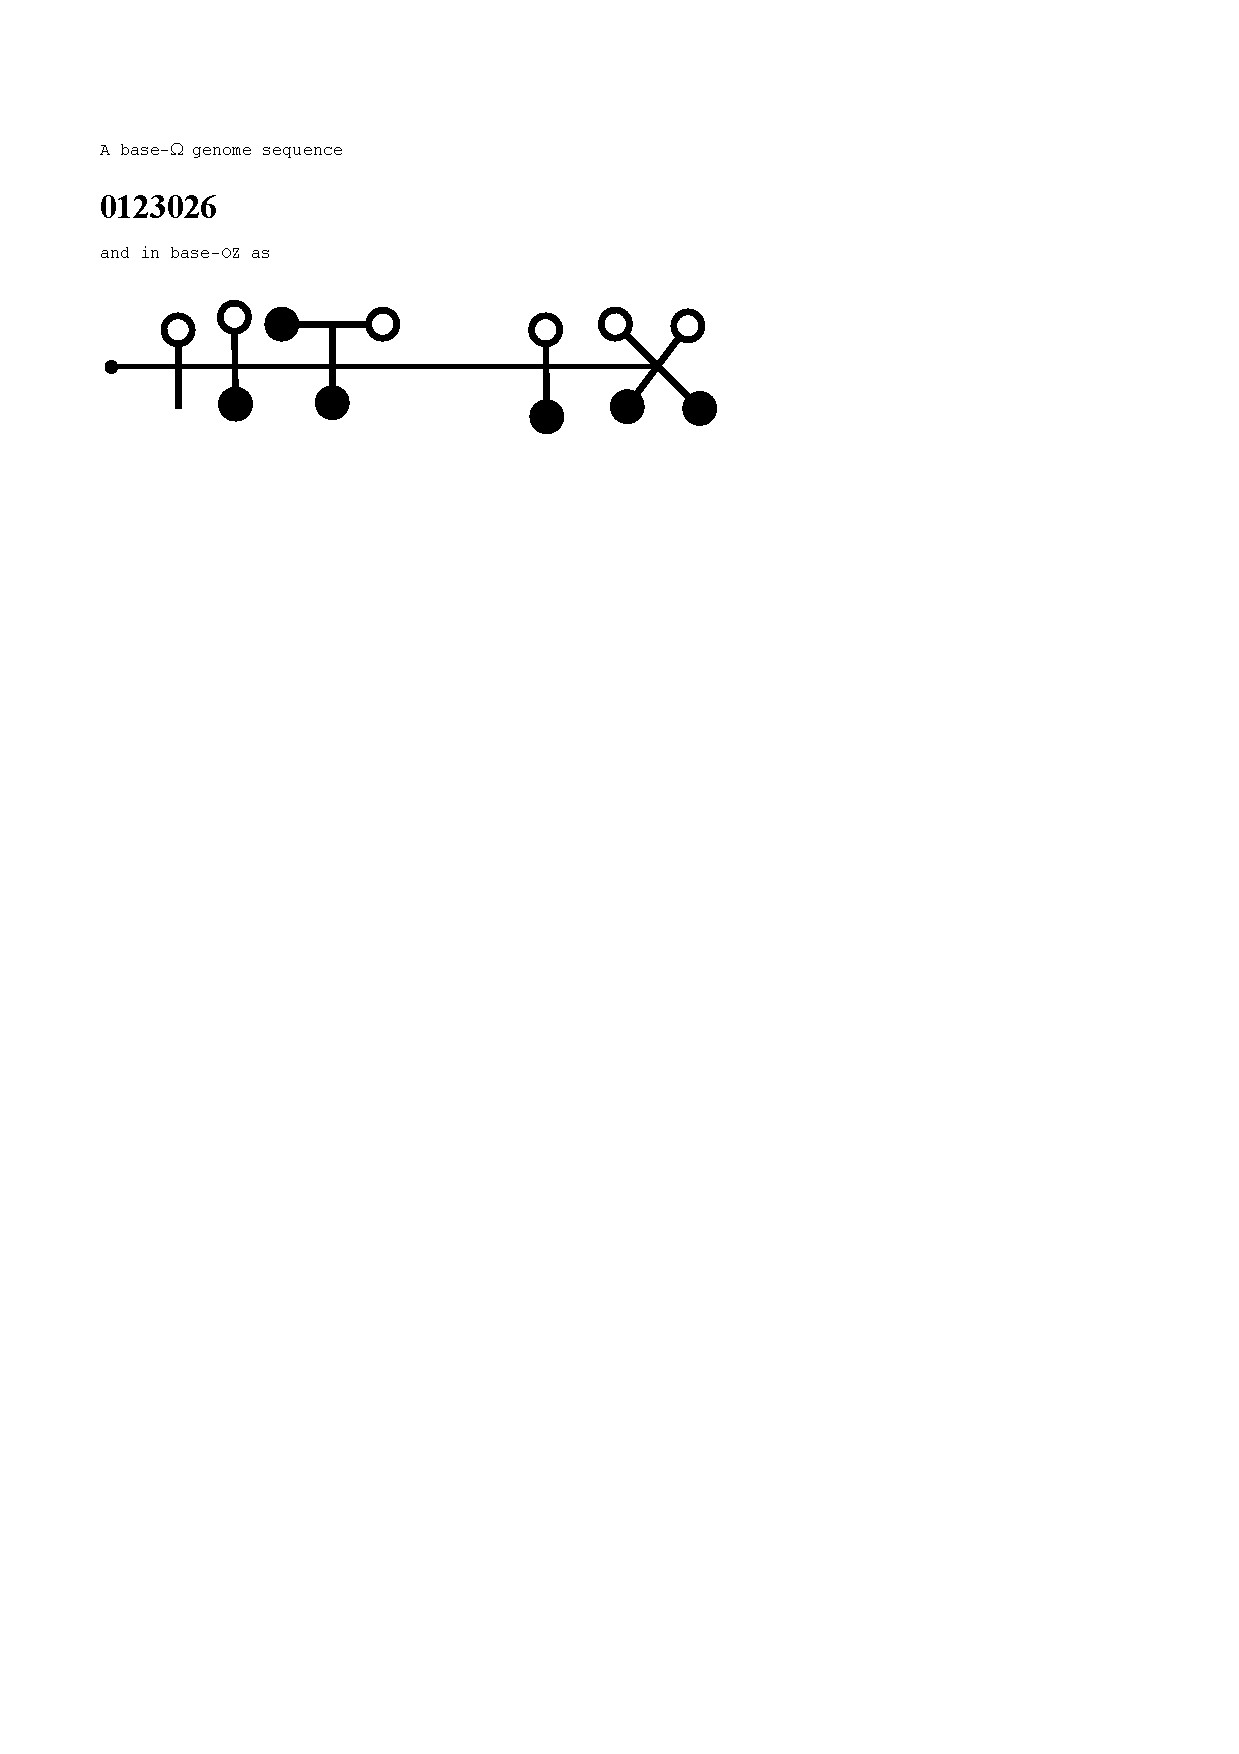
\includegraphics[trim=0cm 22cm 7cm 5cm, clip, width=0.9\textwidth,]{resources/pdfs/OZINCIPHER-APP3-EXA.pdf}\\
   \caption{The equivalent OZIN expression of the $\Omega_{3}$ genome sequence.}
  \label{FIGOZEXA}
  \end{center}
\end{figure}


\subsection{$\Omega$-to-OZIN Genetic Code Transcription Rules}

So, in general, we might sum up our gene transcription rules as such:

\begin{alg}[The \textbf{$\Omega$-to-OZIN Genetic Code Transcription Algorithm}]
\label{ALGCOZIN}

Assuming we have an $\Omega$-base encoded genetic code sequence $\Theta_\Omega$ of some length $n > 0$.

\begin{enumerate}
\item \textbf{INITIALIZE} the transcription by constructing a backbone-structure that's essentially just a line with a dot at the head/start. This is the transcribed sequence $OZ(\Theta_\Omega)$.
\item{\textbf{FOREACH} symbol $\omega_i$ in $\Theta_\Omega$: 
\begin{enumerate}
    \item \textbf{USE} the transcription mapping: $\psi_\Omega \rightarrow \psi_{oz}$ as depicted in \textbf{\hyperref[FIGOZIN]{Figure \ref{FIGOZIN}}}, to \textbf{ENCODE} $\omega_i$  in the equivalent form for the intermediate code.
	\item{\textbf{IF} $\omega_i = 0$:
	\begin{enumerate}
	\item{ \textbf{IF} $OZ(\Theta_\Omega)$ was still empty:
	\begin{enumerate}
		\item Simply \textbf{SKIP} to the next symbol in $\Theta_\Omega$ (loop from \textbf{Step\#2)}.
	\end{enumerate}
		}
		\item{ \textbf{ELSE}: 
		\begin{enumerate}
		\item  \textbf{APPEND}/Insert a GAP in $OZ(\Theta_\Omega)$
		\item \textbf{JUMP} to the next symbol in $\Theta_\Omega$ (loop from \textbf{Step\#2)}.
		\end{enumerate}
		}
	\end{enumerate}
	}
	\item { \textbf{ELSE}:
	\begin{enumerate}
	\item \textbf{APPEND} that encoded version of $\omega_i$ along the backbone structure, $OZ(\Theta_\Omega)$, at the next vacant position ($\leq i$).
	\item \textbf{JUMP} to the next symbol in $\Theta_\Omega$ (loop from \textbf{Step\#2)}.
	\end{enumerate}
	}
\end{enumerate}
}
\item \textbf{TRUNCATE} the backbone-structure after the final term in $OZ(\Theta_\Omega)$.
\item \textbf{RETURN} $OZ(\Theta_\Omega)$ as the final transcribed version of $\Theta_\Omega$ .
\end{enumerate}

\end{alg}



\subsection{Examples of $\Omega$-Genetic Code Transcription}
\label{SECEXAMTRANSC}

So, now that we have the general transcription rules as in \textbf{\hyperref[ALGCOZIN]{Algorithm \ref{ALGCOZIN}}}, we can proceed to explore how to leverage them. 

First, note that, in \textbf{\hyperref[SEC3A]{Chapter \ref{SEC3A}}}, we have looked at not just the interesting idea of [genetic code] sequence complements, but have also explored several applications of the idea in \textbf{\hyperref[SECAPPCOMPLEMENTS]{Section \ref{SECAPPCOMPLEMENTS}}}, including the concept of the equivalence of sequences under the complement transform. Talking of which, assuming we had a special genome sequence that is made up of subsequences that are complements of each other (such as we might call \textbf{palindromic na-Sequences}) --- e.g.\footnote{As in all other uses in this work --- \textit{exempli gratia}} $\Theta_{pal}$ defined below, that is actually a palindrome of the two DNA codons --- \textbf{ATG} (Methionine) and \textbf{CAA} (Glutamine) --- the complements being \textbf{GTA} (Valine) and \textbf{AAC} (Asparagine)\cite{wikipedia_codon_tables}.\\

\begin{equation}
\label{GENOMEPAL}
\Theta_{pal} = \langle A, T, G, C, A, A, A, A, C, G, T, A \rangle
\end{equation}\\

If we express $\Theta_{pal}$ in our special numeric \textbf{base-$\Omega$}, and then into the visual \textbf{base-OZ}, we shall get something like $\Omega_{pal}$\footnote{Simplified, so we can easily visualize it in base-OZ}:\\

\begin{equation}
\label{GENOMEPALOMEG}
\Omega_{pal} = \langle 1, 2, 3, 3, 2, 1 \rangle
\end{equation}\\

And which, if we transcribe it into the intermediate OZIN code, we get:



\begin{figure}[H]
  \begin{center}
  %\includegraphics[trim=2cm 8cm 2cm 8cm, clip, width=0.9\textwidth,]{resources/pdfs/ProteinSynthesisStateMachine.pdf}\\
   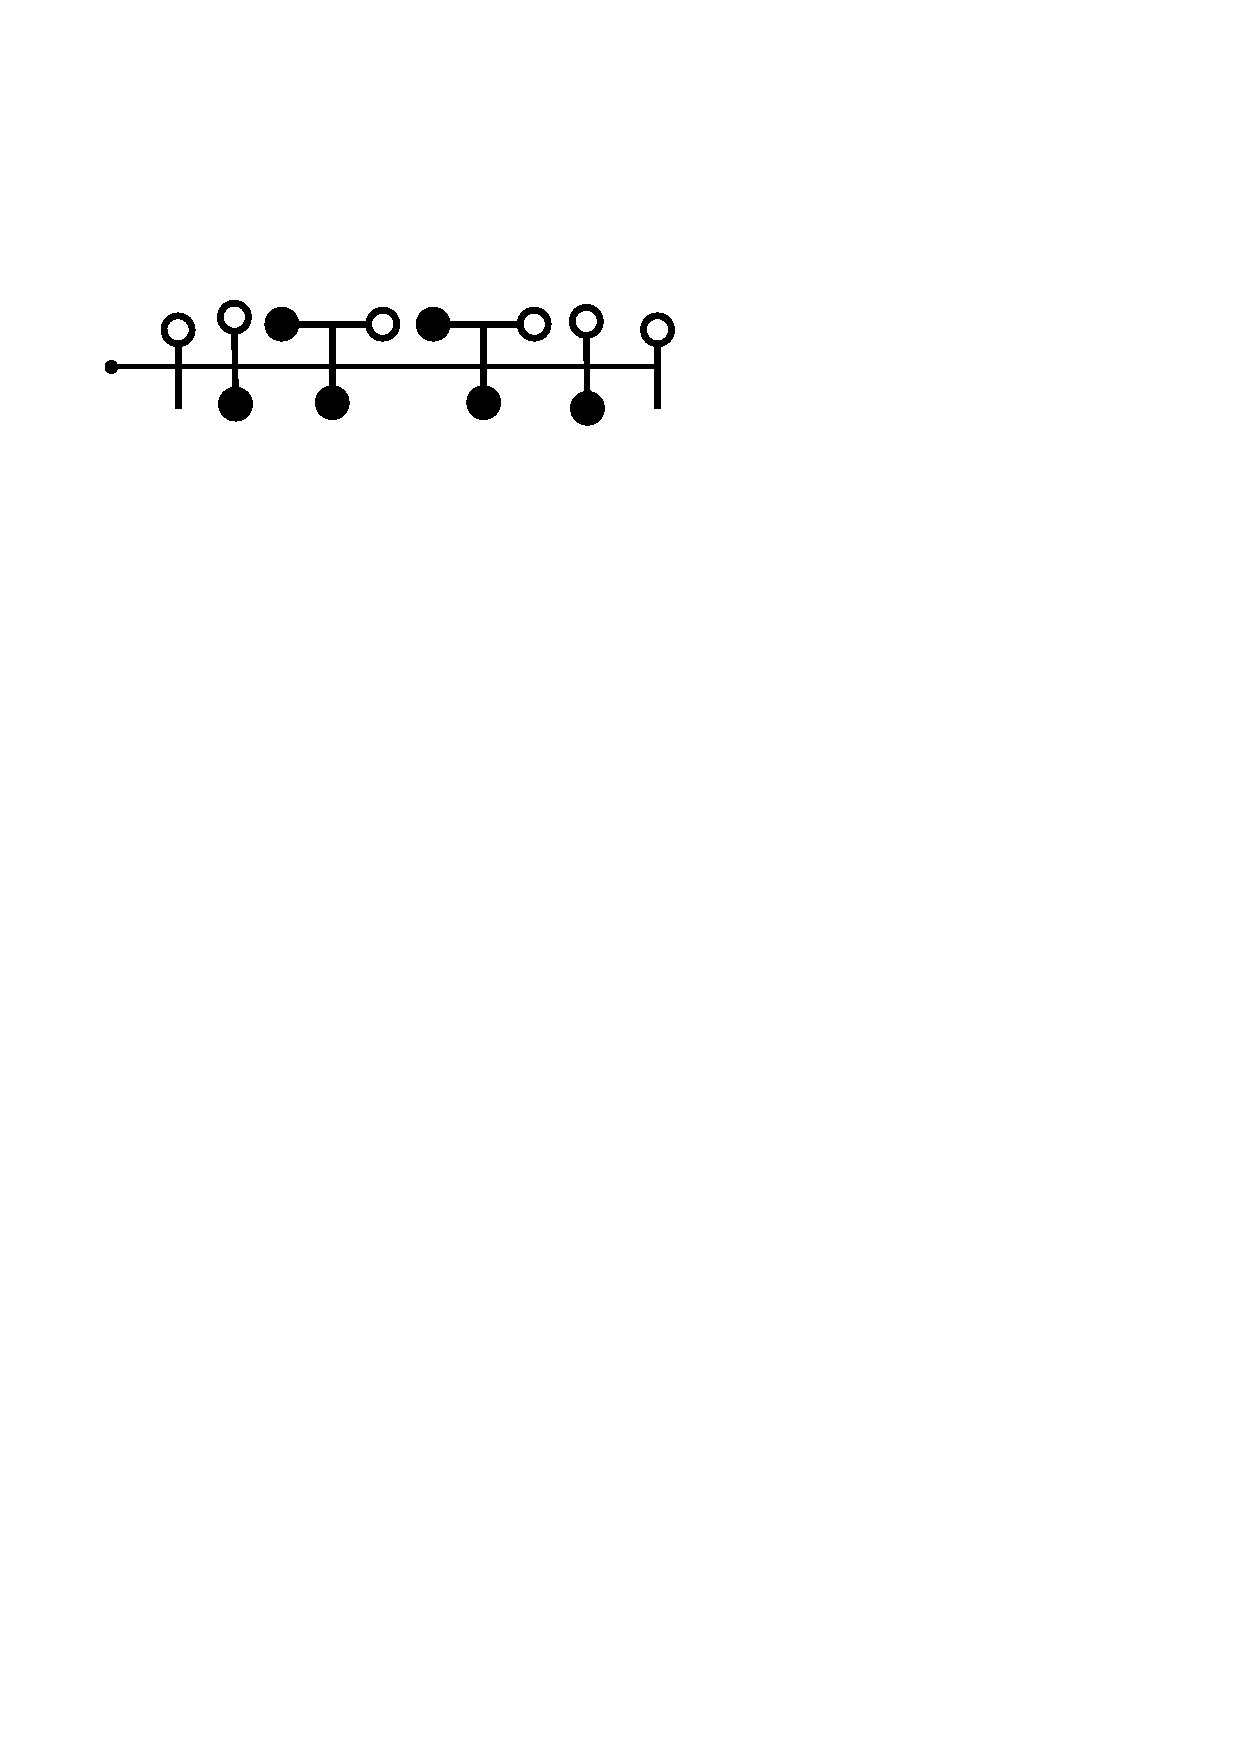
\includegraphics[trim=0cm 22cm 7cm 5cm, clip, width=0.9\textwidth,]{resources/pdfs/OZINCIPHER-APP4-PAL.pdf}\\
   \caption{The palindromic sequence $\Omega_{pal}$ transcribed into base-OZ.}
  \label{FIGOZPAL}
  \end{center}
\end{figure}

Now, notice something interesting here. In particular, if we compare the transcribed forms of $\Omega_{pal}$ and $\Omega_{3}$, we shall notice that even though the two sequences had some differences --- for example, $\Omega_{3}$ contains the ``0" symbol twice, including at the start, and yet, somewhat, because that STOP-codon is skipped during expression/transcription, so we note that, the OZIN-expressions of the two sequences are somewhat similar --- they both share a similar prefix structure, that upon inspection of their genetic code sequences, can be attributed to the 3-gram subsequence ``123".

In fact, this later case is an interesting way to appreciate that even where two organisms, genes or proteins might exhibit significant differences in their appearance or even genetic code, and yet, upon close inspection, we might find some telling signs that they share some \textbf{common-traits}. In this case, we see that the palindromic $\Omega_{pal}$ looks somewhat like the otherwise different $\Omega_{3}$ --- at least in their prefix structures after transcription (and possibly beyond!)

\section{Genetic Code Sequences Processed as Modal Sequence Statistics}
\label{SECGENEXPRE}

Now that we have finished looking at how to express genetic code from its base/storage-form (equivalent to DNA) into its intermediate-form (equivalent to RNA), we can then consider the matter of how that intermediate code eventually gets \textbf{translated} into the final organism\footnote{I say ``final organism" here, because, much as in reality, genome expression might be more complex than merely translating genetic code from DNA into RNA and then final proteins and tissue, and yet, conceptually, that is all there is to it!}.

So, in further advancement our thought experiment concerning genome expression (modeled using hypothetical bio-automata), we shall again utilize the OZIN cipher introduced in \textbf{\hyperref[SECOZIN]{Section \ref{SECOZIN}}}, but shall also introduce another formalism in the form of decoding position within a sequence (such as genetic code in this case), as information about how to express or process the associated symbols. This idea, of leveraging \textit{subtle instructions} embedded in genetic code but which might not be explicit as the actual nucleic acid combinations (such as amino-acid encoding-codons), can be justified when we consider that the genetic code processor (such as the ribosome in our major context --- see \textbf{\hyperref[SEC5]{Section \ref{SEC5}}}), has a way of interpreting sequences not just by what they contain, but also based on the context within which they exist --- or occur to it. 

For example, though generally, the appearance of the RNA codon, \textbf{AAA}, would cause the ribosome to synthesize the corresponding amino-acid Lysine (see \textbf{\hyperref[TAB1]{Table \ref{TAB1}}}), and yet, if such a codon appears in a sequence where no earlier instruction compels the ribosome to START manufacturing a protein, the appearance of that codon shall be useless --- or rather, it shall be interpreted differently merely because of being in the \textit{wrong} context. We saw this in \textbf{\hyperref[SEC05]{Chapter \ref{SEC05}}}, and especially the Ribosome's protein-manufacturing process diagram (\textbf{\hyperref[FIG3]{Figure \ref{FIG3}}}) as well as the State Machine (\textbf{\hyperref[FIG4]{Figure \ref{FIG4}}}) help bring this out clearly. For example, if we modify the gene-program  in \textbf{\hyperref[EQ6]{Equation \ref{EQ6}}} as such:


 \begin{equation}
\label{EQ6B}
\Theta_4^* = \langle \langle A, A, A \rangle, \langle A, U, G \rangle, \langle U, U, A \rangle, \langle U, A, G \rangle \rangle
\end{equation}\\


Then, where we would have expected the ribosome to manufacture a protein whose structure includes the AAA/Lysine amino-acid, the result/effect of our modified sequence shall actually be different from what the original gene-program would have produced. In particular, since the START-codon, AUG (Methionine) appears after AAA, the effective protein to be synthesized would be as equivalent to just the program:

 \begin{equation}
\label{EQ6C}
\Theta_4^* = \langle \langle A, U, G \rangle, \langle U, U, A \rangle, \langle U, A, G \rangle \rangle
\end{equation}\\

Which would produce the protein with just \textbf{UUA}(Leucine) in it! So, positioning of symbols or terms within genetic code does matter, and does encode some important gene or even genome expression information that we can't take for granted, thus the following suggested system for how to express post-RNA genetic code sequences.

\subsection{The Platonic Form Cipher and Position-Sensitive Genetic Code Translation}
\label{SECPLATONIC}

Just like we developed a system for how to map numbers (in base-10) to some non-trivial expressions that we equate to a kind of intermediate genetic code (the OZIN-encoded expressions), we shall similarly start by considering a way to map (still base-10) numbers to spatial-structures\footnote{Especially because, and essentially that, when compared to the code that expresses them, proteins and the organism taken as a whole, \textit{occupy more space} than does just the basic DNA code from which they are expressed.}.

So, with the exception of ``0'', which again is treated as an instruction to `skip' or `stop' within our genome expression system\footnote{Perhaps, and as we shall adopt here, we shall interpret `0', especially \textit{within} and not at the start or end of a sequence, to mean not just a GAP as was the case in \textbf{\hyperref[ALGCOZIN]{Algorithm \ref{ALGCOZIN}}}, but as a JOINT. It somewhat makes biological/anatomical sense.}, we shall adopt the mapping from numbers to spatial-structures as depicted in \textbf{\hyperref[FIGPLATONICCIPH]{Figure \ref{FIGPLATONICCIPH}}} in what we are calling the \textbf{PLATONIC Cipher} System\cite{lutalo_2025_platonic}.


\begin{figure}[H]
  \begin{center}
  %\includegraphics[trim=2cm 8cm 2cm 8cm, clip, width=0.9\textwidth,]{resources/pdfs/ProteinSynthesisStateMachine.pdf}\\
   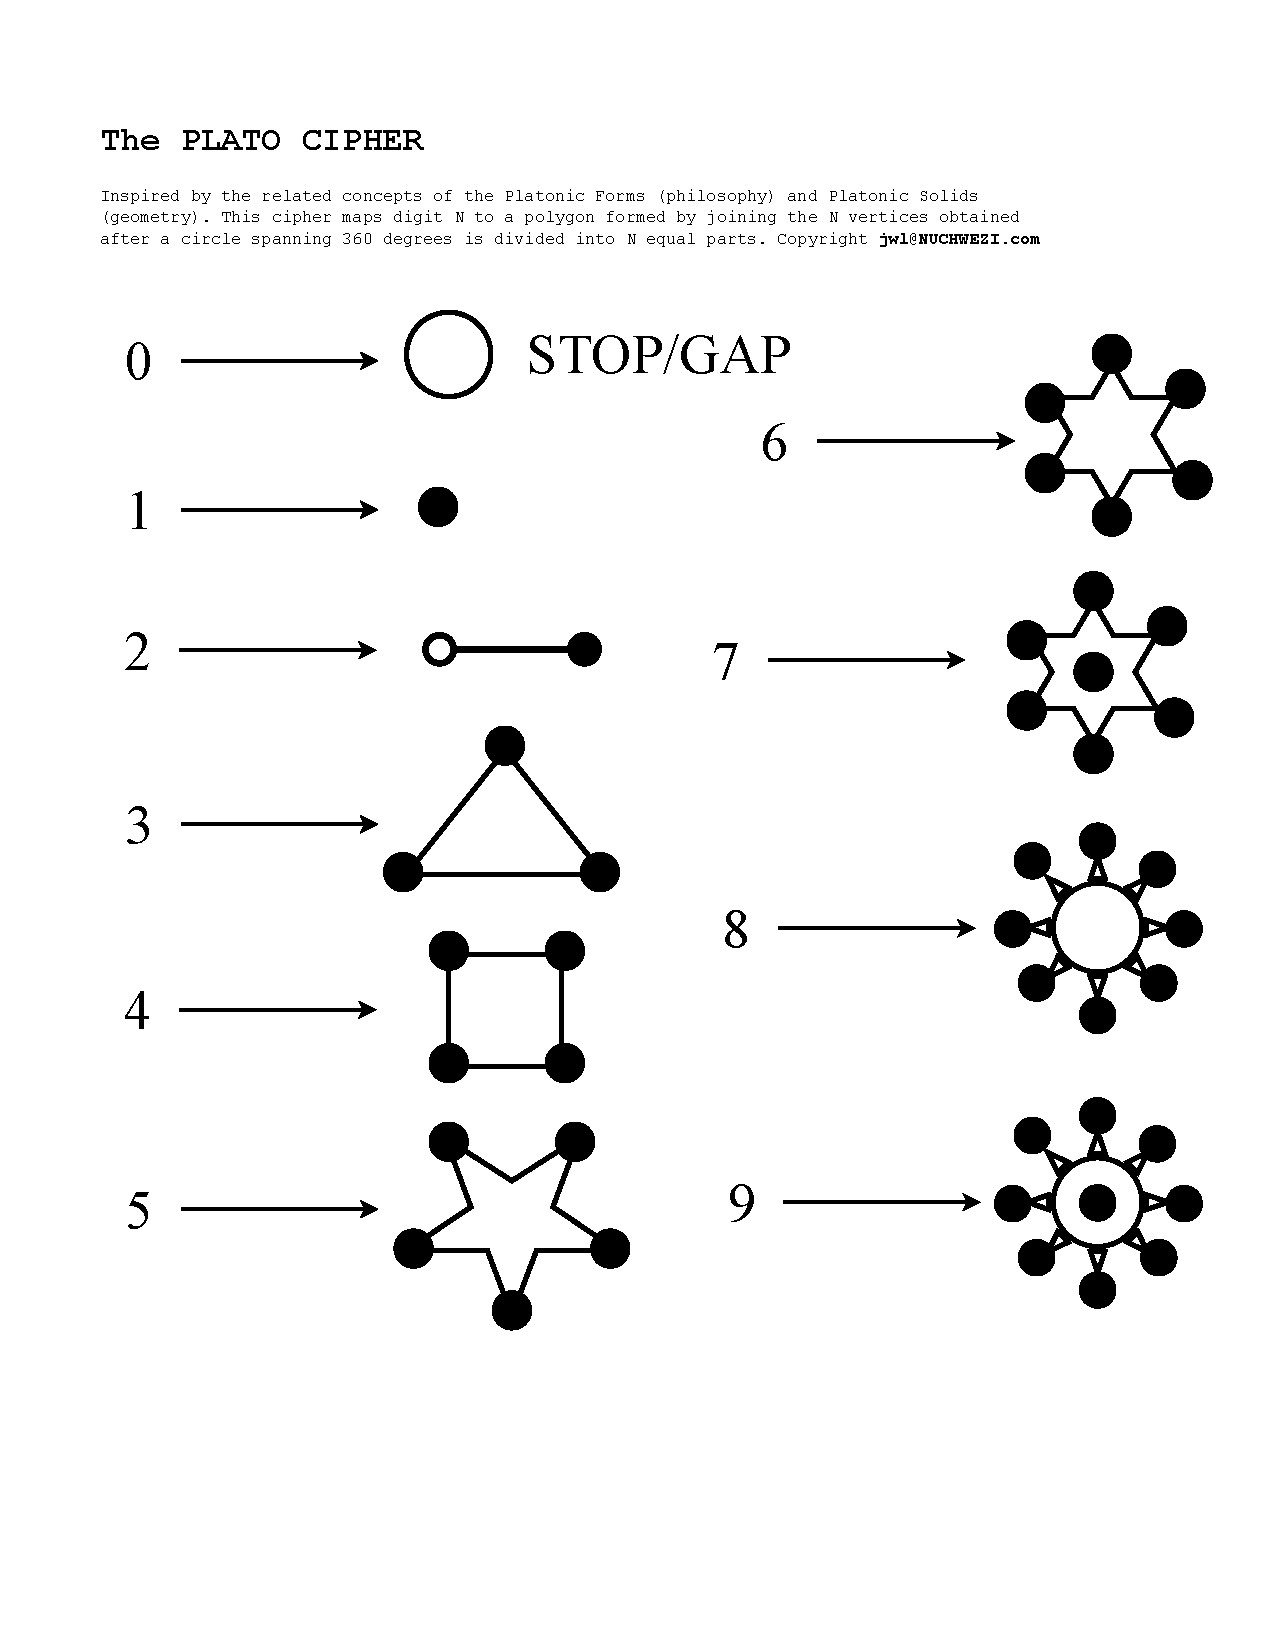
\includegraphics[trim=0cm 4cm 0cm 0cm, clip, width=0.9\textwidth,]{resources/pdfs/PLATOCIPHER.pdf}\\
   \caption{The PLATONIC Cipher\cite{lutalo_2025_platonic} a mapping from Decimal Symbols (our base-$\Omega$) to Spatial-Geometric Forms ($\psi_{pf}$).}
  \label{FIGPLATONICCIPH}
  \end{center}
\end{figure}


How does it work?

\subsection{$\psi_{\Omega}$-to-$\psi_{pf}$: PLATONIC Form Genetic Code Translation Rules}
\label{SECGENSEQEXPRES}


So, in general, we might sum up our start to finish gene (and genome) expression protocol with the post-transcription rules and process as such:

\begin{alg}[The \textbf{$\Omega$-to-PLATONIC Form Genetic Code Expression Algorithm}]
\label{ALGCOZINPLATO}

Assuming we have an $\Omega$-base encoded genetic code sequence $\Theta_\Omega$ of some length $n > 0$.

\begin{enumerate}
    \item{\textbf{INITIALIZE} the expression with a transcription, by Using \textbf{\hyperref[ALGCOZIN]{Algorithm \ref{ALGCOZIN}}} to \textbf{CONSTRUCT} the \textbf{Intermediate Form Affix} (IFA) of $\Theta_\Omega$ --- essentially return $OZ(\Theta_\Omega)$ as the start of the \textbf{Final Genome Expression} (FGE) $\boxed{OZ(\Theta_\Omega)}^*$ --- so that the final complete expressed(transcribed+translated ) sequence shall be as:\\

\begin{equation}
\label{EQTRANSLGENSEQ}
\boxed{OZ(\Theta_\Omega)}^* = OZ(\Theta_\Omega)\cdot\boxed{OZ(\Theta_\Omega)}
\end{equation}\\

$\boxed{OZ(\Theta_\Omega)}: \mathbb{N} \times \psi_{pf}$ is the suffix of expressed na-Sequence $\Theta_\Omega$, and is expressed in our genome expression system, as PLATONIC-Form encoded \textbf{modal sequence statistic} of $OZ(\Theta_\Omega)$\footnote{We render the \textbf{suffix of FGE} as $\overset{>}{OZ(\Theta_\Omega)}$ because it allows us to not express $\Theta_\Omega$ naively at the genome or gene level, but also, so that, from an information-theoretic perspective, the completed genome expression is somewhat a statistical summary of what the genome sequence contains --- the appearance of an animal or a plant or virus, depicting or expressing the summary of its DNA code. We do this then, by not merely doing a 1-to-1 translation of the intermediate Ozin-code expression $OZ(\Theta_\Omega)$, but instead computing its summary in form of $\overset{>}{OZ(\Theta_\Omega)}$, and then instead translating that into the final spatial/geometric forms as per $\psi_{pf}$. This shall complete the entire processing/synthesis of sequence $\Theta_\Omega$, or rather our genome expression.} --- the \textbf{PFA}\footnote{Platonic Form Aspect}, i.e.:\\

\begin{equation}
 \boxed{OZ(\Theta_\Omega)} = \boxed{\overset{>}{OZ(\Theta_\Omega)}}_{pf}
\end{equation}\\


}
\item{ So, once we have the \textbf{IFA}, $OZ(\Theta_\Omega)$, \textbf{PROCEED} to use it to generate the rest of the sequence expression as follows: 
\begin{enumerate}
\item {\textbf{INITIALIZE} FGE, $\boxed{OZ(\Theta_\Omega)}^*$ as just:\\

\begin{equation}
\label{EQSTARTFGE}
\boxed{OZ(\Theta_\Omega)}^* = \langle \langle OZ(\Theta_\Omega) \rangle \langle \rangle \rangle
\end{equation}\\

This ensures, we have the prefix affix, \textbf{IFA}, as the contents of the sequence start of \textbf{FGE} \textit{extended} by a \textbf{still empty subsequence} --- in expression form, this shall merely be a backbone structure with \textbf{IFA} as its head, and a terminal that is ready to have more units appended to it, \textbf{after a single GAP/JOINT extension to IFA}. So, it also means, at this juncture, \textbf{PFA} is just:\\

\begin{equation}
\label{EQSTARTFGESUF}
\boxed{OZ(\Theta_\Omega)} = \langle \rangle
\end{equation}\\

}
\item {
	\textbf{COMPUTE} the \textbf{IFA MSS}, $\overset{>}{OZ(\Theta_\Omega)}$
}
\item {
	\textbf{COMPUTE} $m$, the cardinality of the \textbf{IFA MSS}, $m = \invpi(\overset{>}{OZ(\Theta_\Omega)})$
}
\item {
	\textbf{COMPUTE} the \textbf{Platonic Form Encoding Key}(PFEK), $\boxed{\psi_{pf}}_m$, corresponding to $m$ and based on the \textbf{SLSA Algorithm}\footnote{The \textbf{SLSA}, \textbf{Second Lu-Shuffle Algorithm} is well introduced and explained in \textbf{\hyperref[APPSLSA]{Section \ref{APPSLSA}}}, and it basically is about generating an exact anagram of the input sequence, corresponding to a particular partitioning index --- in this case (and by \textbf{LGES} convention, denoted), $m$, the size of the \textbf{IFA MSS}.}
}
\item{\textbf{FOREACH} symbol/term $\omega_i^*$ in \textbf{IFA MSS}, $\overset{>}{OZ(\Theta_\Omega)}$: 
\begin{enumerate}
    \item{\textbf{USE} the \textbf{symbol set translation mapping}: $\psi_\Omega \rightarrow \boxed{\psi_{pf}}_m \rightarrow \psi_{pf}$ where that final term corresponds to the mapping depicted in \textbf{\hyperref[FIGPLATONICCIPH]{Figure \ref{FIGPLATONICCIPH}}}, to translate $\omega_i^*$ into the equivalent \textbf{Platonic Form}, $\boxed{\omega_i^*}$, for the final expression as such:}
\item { \textbf{IF} $\omega_i^* \equiv 0$:Operating on the current \textbf{FGE}: 
		\begin{enumerate}
		\item { \textbf{APPEND}/Insert a JOINT onto \textbf{FGE},  $\boxed{OZ(\Theta_\Omega)}^*$\\

		\begin{equation}
		\label{EQEXTFGEJOINT}
		\boxed{OZ(\Theta_\Omega)}^* = \boxed{OZ(\Theta_\Omega)}^* \cdot \boxed{\omega_i^*}_{joint}
		\end{equation}\\		
		
		And equivalently/thus:\\
		
		\begin{equation}
		\label{EQEXTFGEJOINTSUF}
		\boxed{OZ(\Theta_\Omega)} = \boxed{OZ(\Theta_\Omega)} \cdot \boxed{\omega_i^*}_{joint}
		\end{equation}\\				
		
		}
		\item \textbf{PROCEED} to the next symbol in \textbf{IFA MSS}, $\overset{>}{OZ(\Theta_\Omega)}$\\ (loop from \textbf{Step\#2(e))}.
		\end{enumerate}
	}
	\item { \textbf{ELSE}: \textbf{RESOLVE} the correct  $\boxed{\omega_i^*}$  for  $\omega_i^*$  by using the relation\footnote{Concerning how to actually arrive at the correct $\boxed{\omega_i^*}$ via the correct $\boxed{\psi_\Omega}_m$ for a given \textbf{IFA MSS}, refer to \textbf{\hyperref[SECIFAMSSPFMAPS]{Appendix \ref{SECIFAMSSPFMAPS}}} that covers how to compute or look-up the necessary \textbf{platonic form encoding key}.}\\


\fbox{
\begin{minipage}{0.9\textwidth}

\begin{equation}
\label{EQFBOXED}
 \boxed{\omega_i^*} = \rho_j \in \psi_{pl} +  j \times \omega_i^* : j = \boxed{j} : I(\boxed{j},\boxed{\psi_{pf}}_m) = I(\omega_i^*,\overset{>}{OZ(\Theta_\Omega)})
\end{equation}\\

\end{minipage}}
\\



	\begin{enumerate}
        \item{\textbf{PLACE} that encoded version, $\boxed{\omega_i^*}$, along the existing \textbf{FGE} structure at the next vacant position ($\invpi(\Theta_\Omega)+i$). Expressible with another version of \textbf{\hyperref[EQEXTFGEJOINT]{Equation \ref{EQEXTFGEJOINT}}} as:\\
	
	\begin{equation}
	\label{EQEXTFGEPF}
		\boxed{OZ(\Theta_\Omega)}^* = \boxed{OZ(\Theta_\Omega)}^* \cdot \boxed{\omega_i^*}
		\end{equation}\\
		
		And equivalently:\\
		
		\begin{equation}
		\label{EQEXTFGEPFSUF}
		\boxed{OZ(\Theta_\Omega)} = \boxed{OZ(\Theta_\Omega)} \cdot \boxed{\omega_i^*}
		\end{equation}\\
		
            Where the special \textbf{PFA} term, $\boxed{\omega_i^*}$, as per \textbf{\hyperref[EQFBOXED]{Equation \ref{EQFBOXED}}}, is basically the PLATONIC Form corresponding to position $j$ in $\boxed{\psi_{pf}}_m$ --- an \textbf{anagrammatized $pf$-symbol set} relative to $m$ and which is used to look-up the \textbf{correct indices} for the \textbf{corresponding} geometric structure components from $\psi_{pf}$, the symbol set of the final form of the \textbf{PFA}, but also with the \textit{twist} that the intermediate form $\omega_i^*$ is attached to that geometric structure $j$ times --- as depicted in example\footnote{It shall be interesting to note, that based on the \textbf{PFEK} by \textbf{SLSA} --- see \textbf{\hyperref[TABSSLAPERK]{Table \ref{TABSSLAPERK}}}, that assuming we had [an actually \textit{strange}] organism whose equivalent $\Omega$-encoded DNA sequence were just the sequence $\Theta$ = \textbf{666}, its corresponding \textbf{IFA} characteristic would be just $\hbar(\overset{>}{\Theta}) = $\textit{\textbf{6}3}, the corresponding \textbf{MSS} just $\langle$\textbf{6}$\rangle$, and so its \textbf{PFEK} look-up key, $m = \invpi(\overset{>}{\Theta}) = 1$, so that, its corresponding $\boxed{\psi_{pf}}_1 = \langle 4 \rangle$, and so that for its \textbf{BODY} component in the associated full genome expression, the entire \textbf{PFA} would just be $\boxed{\omega_1^*} \implies 4_{pf} \otimes 6_{oz}$ --- which is exactly what we see in this picture in \textbf{\hyperref[FIGEXAPLATONICFORMPFA]{Figure \ref{FIGEXAPLATONICFORMPFA}}}!} \textbf{\hyperref[FIGEXAPLATONICFORMPFA]{Figure \ref{FIGEXAPLATONICFORMPFA}}}, with each expression of $\omega_i^*$ attached to one of the $j$ \textbf{appendage spots} on the shape for $\boxed{\omega_i^*}$.
	}
	\item \textbf{PROCEED} to the next symbol in \textbf{IFA MSS}, $\overset{>}{OZ(\Theta_\Omega)}$\\ (loop from \textbf{Step\#2(e))}.
	\end{enumerate}
	}
\end{enumerate}
}
\end{enumerate}
}

\item \textbf{TRUNCATE} the final-structure after the final term in \textbf{FGE}.
\item \textbf{RETURN} \textbf{FGE}, $\boxed{OZ(\Theta_\Omega)}^*$ as the final transcribed and translated version of $\Theta_\Omega$. The culmination of our conceptual genome expression.
\end{enumerate}
$\qed$
\end{alg}


\begin{figure}[H]
  \begin{center}
   %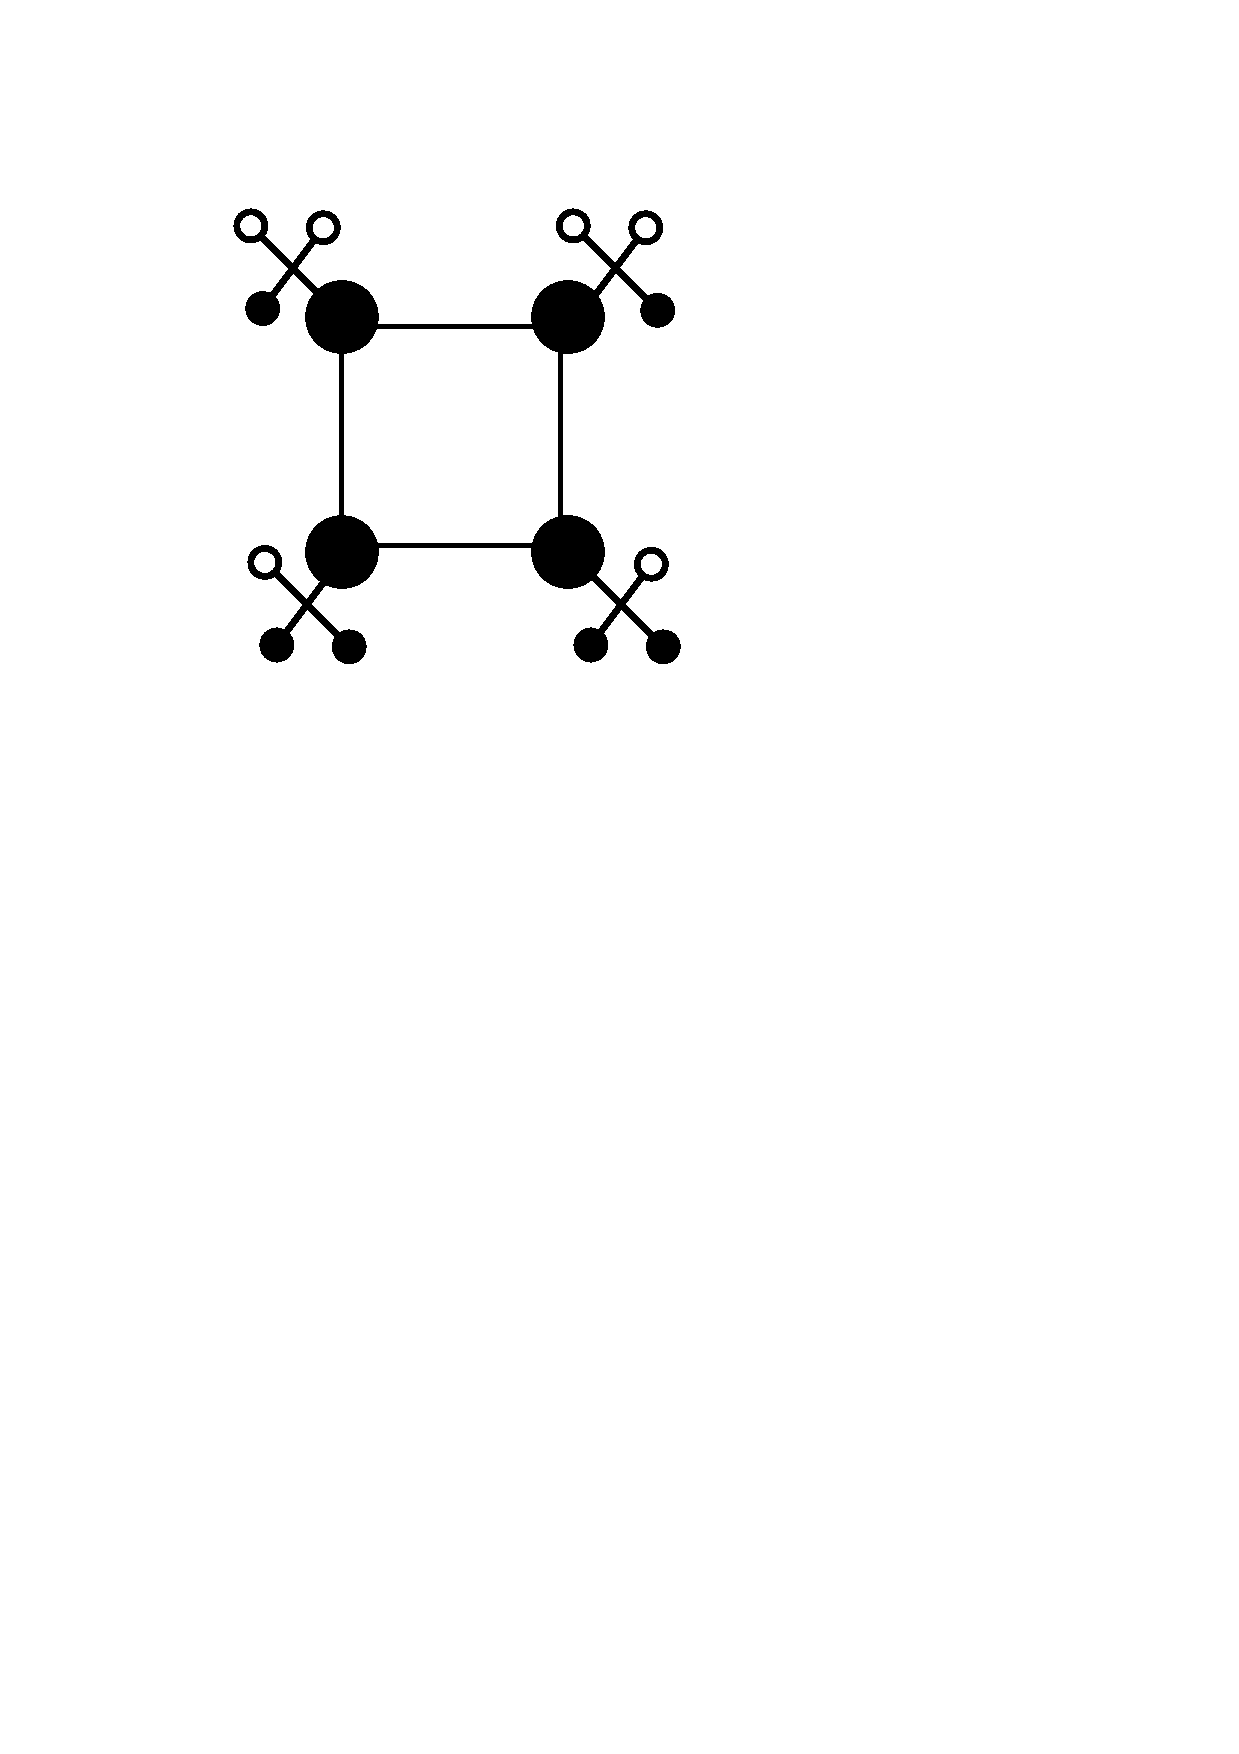
\includegraphics[trim=LEFT BOTTOM RIGHT TOP, clip, width=0.9\textwidth,]{resources/pdfs/EXAPLATONICFORM-PFA.pdf}\\
   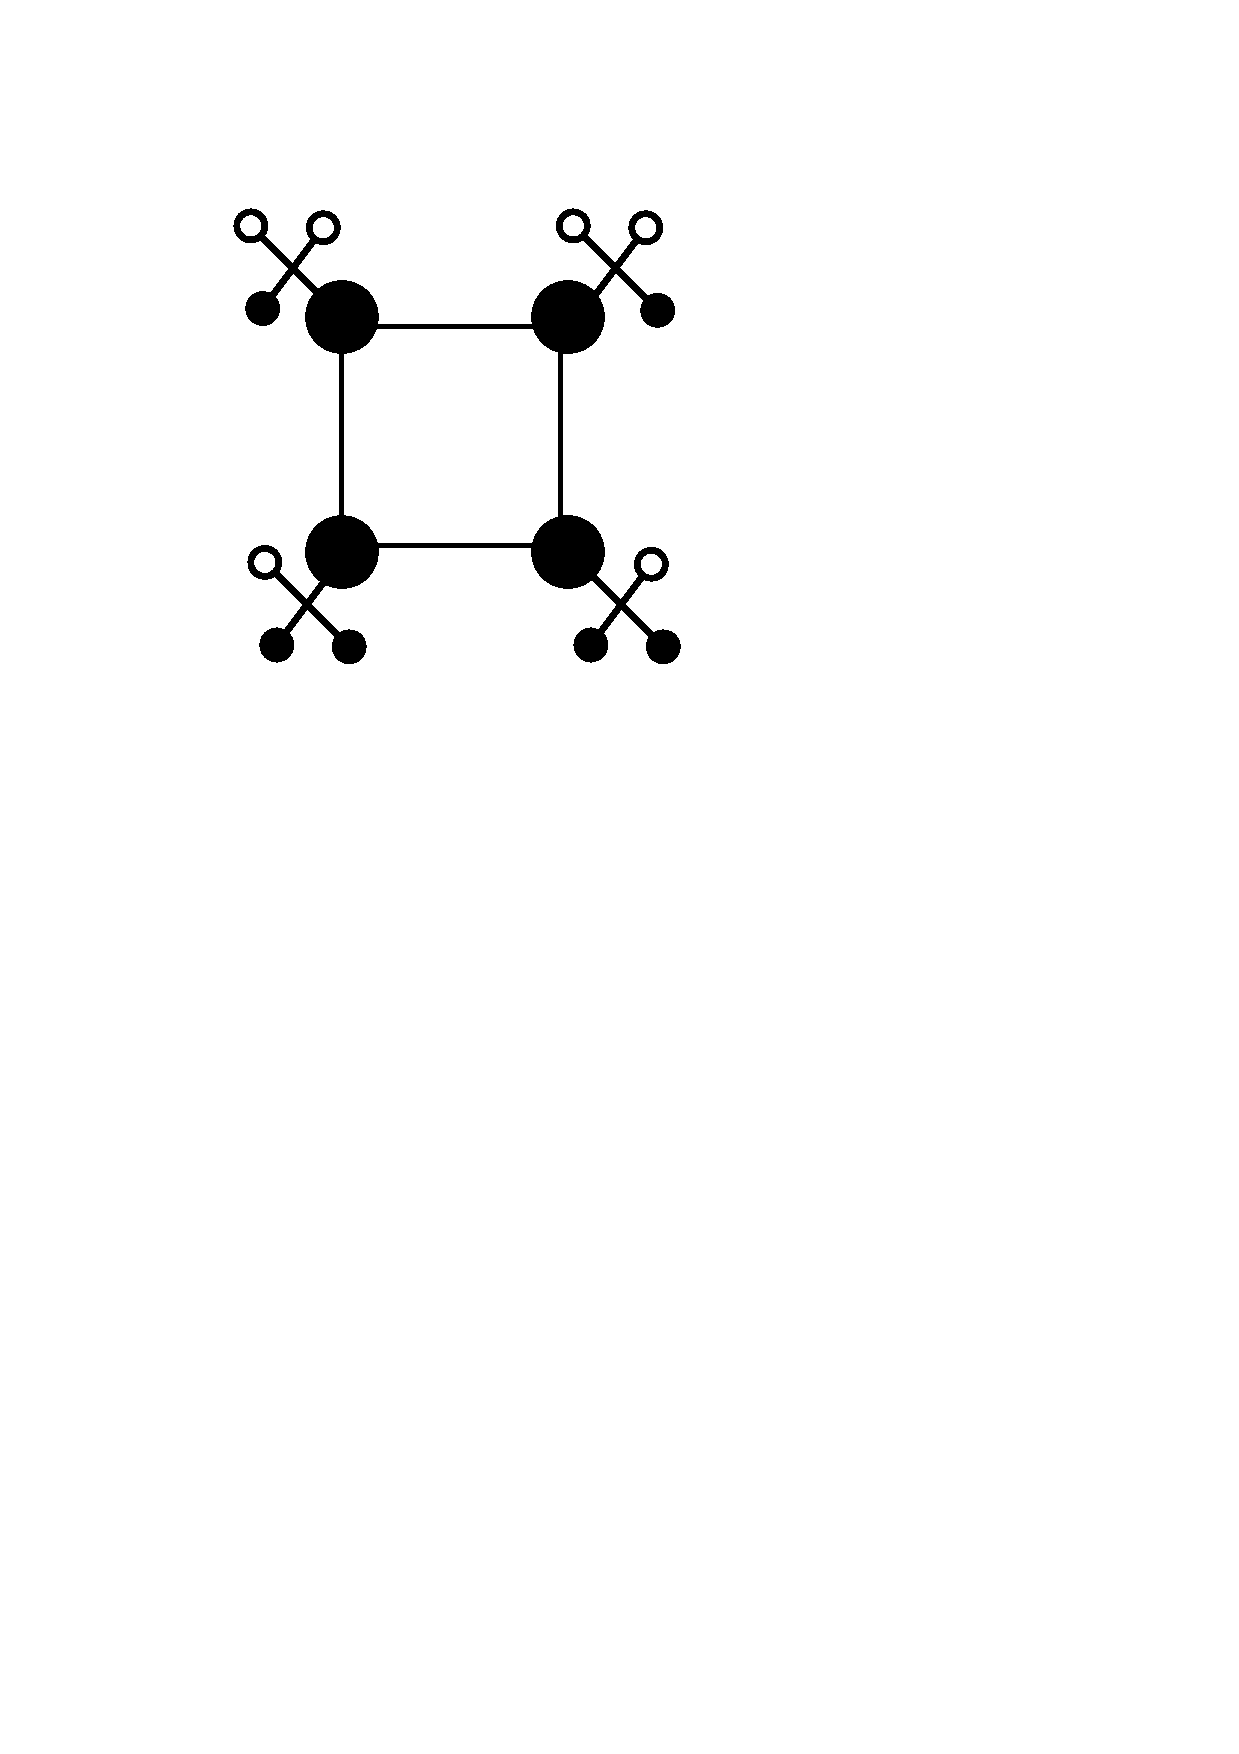
\includegraphics[trim=3cm 18cm 8cm 3cm, clip, width=0.9\textwidth,]{resources/pdfs/EXAPLATONICFORM-PFA.pdf}\\
   \caption{An example of a single \textbf{amino-acid} or rather, the \textbf{PFA} component of a \textbf{FGE} equivalent to one \textbf{amino-acid} segment expressed using the \textbf{LGES} system. This particular expression corresponding to a rendering of the configuration \textbf{$4_{pf} \otimes 6_{oz}$} = \textbf{$4_{pf} + 4 \times 6_{oz}$}.}
  \label{FIGEXAPLATONICFORMPFA}
  \end{center}
\end{figure}



After looking at some examples of actual genome expressions rendered using the \textbf{LGES}, perhaps most reviewers of \textbf{\hyperref[ALGCOZINPLATO]{Algorithm \ref{ALGCOZINPLATO}}} shall come to appreciate that it is not only non-trivial, but is likewise plausible given the sensibilities of how actual expression occurs in nature/reality\footnote{That said, it shall be up to others --- botanists, zoologists, molecular biologists, virologists, etc. to either confirm or refute whether or not \textbf{LGES} does indeed echo the reality in nature or whether it is a theory only applicable to a subsection of reality --- \textit{which, if not all?}} --- see a natural expression as in \textbf{\hyperref[FIGPINEAPPLE]{Figure \ref{FIGPINEAPPLE}}}, and that it encapsulates the ideals of both distinctiveness but also diversity for the minutest of organic creatures that are just as basic as mere genetic code with a basic encapsulating body (such as viruses), but also complex organisms belonging to distinct families of prokaryotes and eukaryotes.


\subsection{Examples of Complete Lu-Genome Expressions}
\label{SECFULLGES}


We get to see the first example of the output of processing some na-Sequence expressed originally in base-$\Omega$ such as for $\Omega_{3}$ from \textbf{\hyperref[EQDNEXA]{Equation \ref{EQDNEXA}}}, in its final expression form as in \textbf{\hyperref[FIGPLATONICEXA]{Figure \ref{FIGPLATONICEXA}}}\cite{lutalo_2025_exa} --- more importantly, since we have already seen its \textbf{IFA} (the \textbf{FGE} prefix) in \textbf{\hyperref[FIGOZEXA]{Figure \ref{FIGOZEXA}}}, we note that, we essentially see the update as the result of expressing the entire \textbf{FGE} via the \textbf{IFA MSS} equivalent to the following derivation transformation:

\begin{center}
\fbox{
\begin{minipage}{\textwidth}

\begin{trans}
\label{TRANSFGEDERIV}
$\Omega_{3} = \langle 0,1,2,3,0,2,6 \rangle \rightarrow \overset{>}{\Omega_{3}} = \langle 0, 2, 1, 3, 6 \rangle$\\
$ \implies m = \invpi(\overset{>}{\Omega_{3}}) = 5 \implies  \boxed{\psi_{pf}}_5 = \langle 2, 1, 0, 6, 8 \rangle$\\ 
$\implies \boxed{OZ(\Omega_{3})} = \langle 2_{pf} \otimes 0_{oz}, 1_{pf} \otimes 2_{oz}, 0_{pf} \otimes 1_{oz}, 6_{pf} \otimes 3_{oz}, 8_{pf} \otimes 6_{oz} \rangle$\\\\
$ \approx \langle GAP, 1_{pf} \otimes 2_{oz}, GAP, 6_{pf} \otimes 3_{oz}, 8_{pf} \otimes 6_{oz} \rangle$\\\\
$\implies \boxed{OZ(\Omega_{3})}^* = \langle 0,1,2,3,0,2,6 \rangle_{oz} \cdot \langle GAP, 1_{pf} \otimes 2_{oz}, GAP, 6_{pf} \otimes 3_{oz}, 8_{pf} \otimes 6_{oz} \rangle$
\end{trans}


\end{minipage}}
\\
\end{center}


The corresponding complete rendered \textbf{FGE} for $\Omega_{3}$ would then be as shown in \textbf{\hyperref[FIGPLATONICEXA]{Figure \ref{FIGPLATONICEXA}}}.



\begin{figure}[H]
  \begin{center}
  %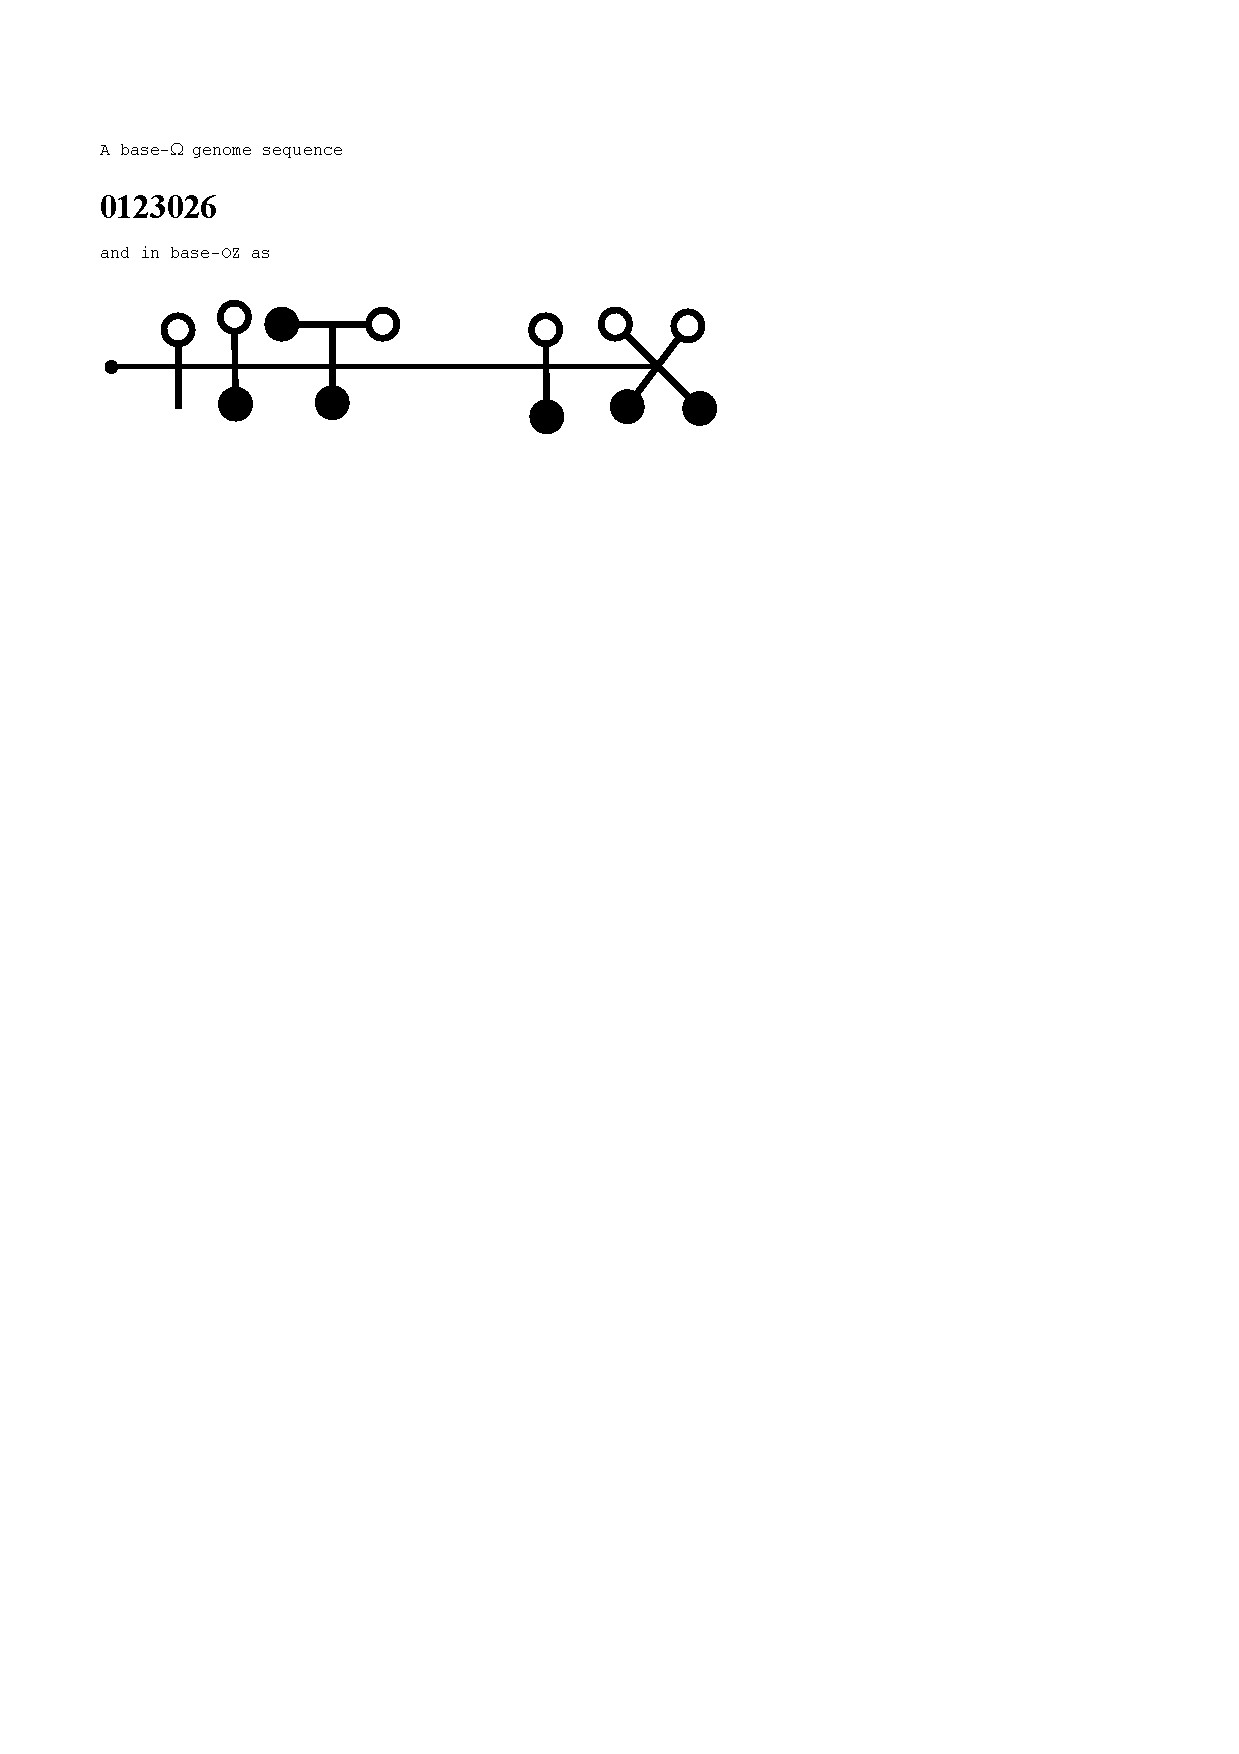
\includegraphics[trim=0cm 20cm 0cm 0cm, clip, width=0.9\textwidth,]{resources/pdfs/OZINCIPHER-APP3-EXA.pdf}\\
   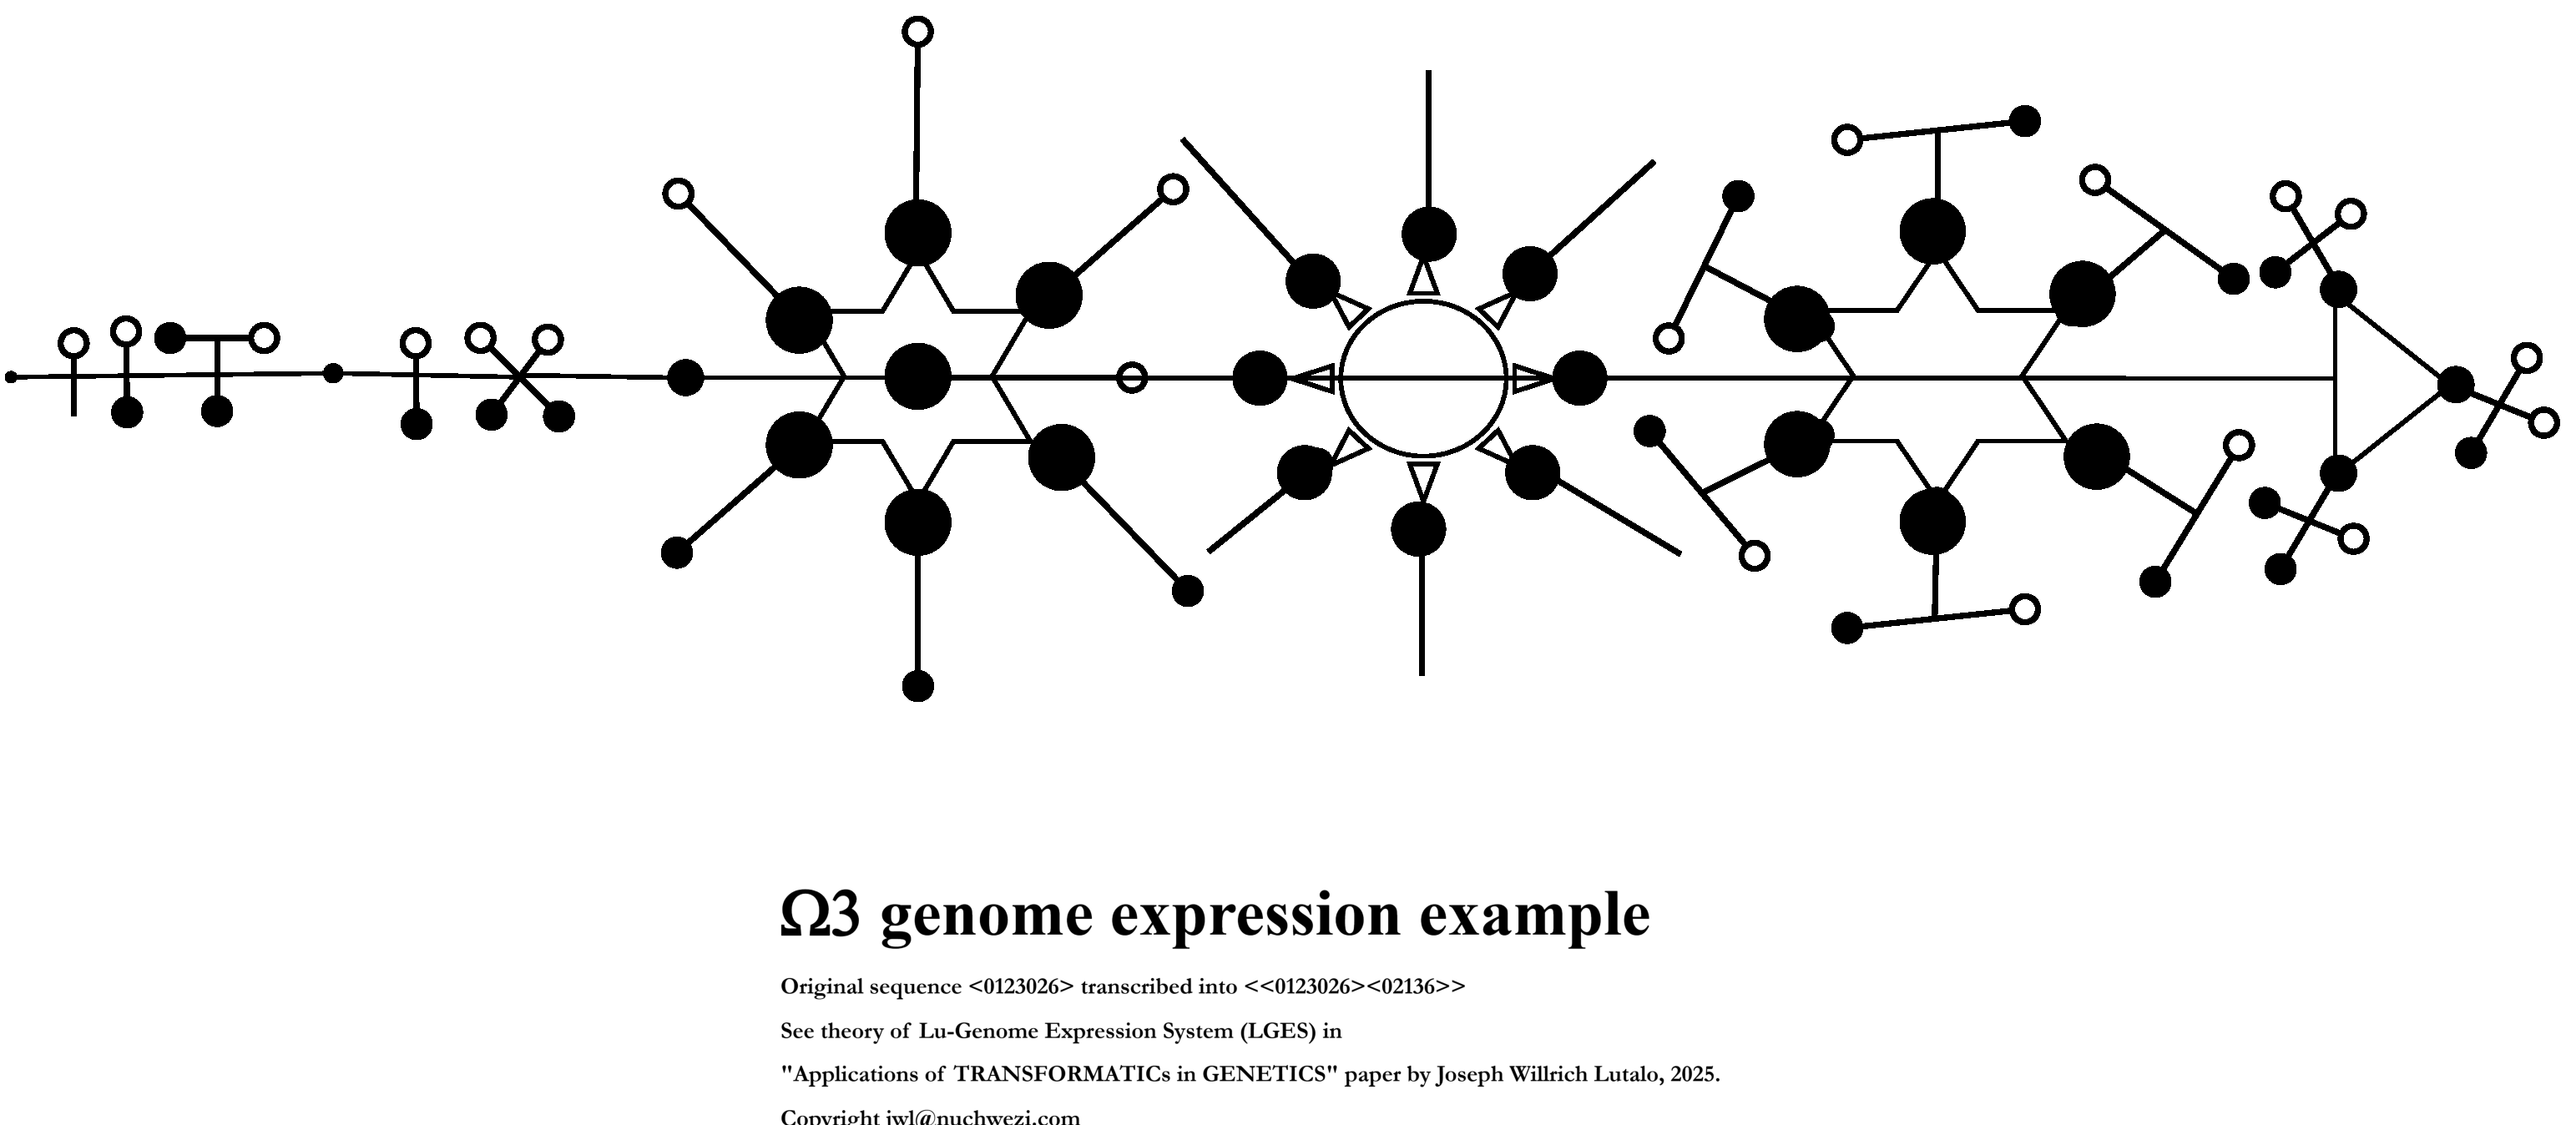
\includegraphics[trim=0cm 0cm 0cm 0cm, clip, width=0.9\textwidth,]{resources/pdfs/PLATONIC-EXA-landscape.pdf}\\
      \caption{The equivalent LGES complete genome expression of the $\Omega_{3}$ genome sequence (from \textbf{\hyperref[EQDNEXA]{Equation \ref{EQDNEXA}}})}
  \label{FIGPLATONICEXA}
  \end{center}
\end{figure}


Though we won't delve into exploring all kinds of possible \textit{interesting} scenarios with regards to the \textbf{LGES}, we can look at one other example and then move on. Also, it shall be interesting and worth noting --- especially for those who wish to explore the \textbf{LGES} algorithm, that a mathematical derivation such as depicted in \textbf{\hyperref[TRANSFGEDERIV]{Transformation \ref{TRANSFGEDERIV}}}, captures the gist of all there is to \textbf{LGES}, and that any other case can merely adapt such a formalism so as to arrive at the visual/pictorial expression of some $\Omega$-encoded genetic or arbitrary sequence.


From the example hypothetical genome sequences we have encountered, perhaps let us revisit \textbf{\hyperref[EQDNAV]{Equation \ref{EQDNAV}}} and see what the \textbf{Euler Virus} might look like when fully expressed in our system.

So, first of all, note that we already did the first-leg of \textbf{\hyperref[ALGCOZINPLATO]{Algorithm \ref{ALGCOZINPLATO}}}, and we have seen what the \textbf{FGE} prefix --- the \textbf{IFA}, would look like in \textbf{\hyperref[FIGOZEVIRUS]{Figure \ref{FIGOZEVIRUS}}}\footnote{\textbf{FUTURE WORK}: Talking of which, for the well-read reader, and especially students and explorers of not just esoteric languages but especially occult languages and systems --- perhaps better we talk of \textbf{Occult Philosophy}\cite{agrippa2014occult}, not only the coincidence that our OZIN-expressions look indeed \textit{occult} --- such as one might find utilized in occult systems such as John Dee's Enochian\cite{lutalo2025unraveling}, but also that both the \textbf{IFA} and \textbf{PFA} --- the later, expressed in a somewhat more familiar (because the polygons at the core of the PF-cipher are indeed commonplace in both mathematics and mysticism) language, but ultimately, the experienced observer might appreciate that complete \textbf{LGES} expressions/figures such as \textbf{Figure \ref{FIGPLATONICEXA}} look much like the traditional/ancient mystical glyphs known as \textbf{Mandalas}(\textit{oriental esotericism}) to modern scholars such as Carl G. Jung that enjoyed these subjects\cite{jung1964symbols} and perhaps, and as the author himself has explored in works such as the novel ``Rock `N' Draw"\cite{lutalo2025rock}, these figures so much remind one of \textbf{Voodoo Veves} --- in that novel, depicted as enchantment geomantic/geomancy forms! Perhaps, in a later work on either philosophy or mysticism by the author --- see earlier works of this kind in \cite{lutalo2025concerning_trans}, we shall want to take time off and properly explore this exciting dimension of human expression and culture, especially since, unlike what might have ever come before, our symbolic programs, unlike voodoo veves (\textit{african esotericism}) or chaos magick sigils (\textit{western esotericism}), are rooted in two objective fields of inquiry --- mathematics and biology (and not mere speculation) --- thus we might even start talking of \textbf{genetic veves}. And no, though the acronym \textbf{IFA} reminds one of the \textit{Ifa} esoteric system of  Western Africa, and yet, the author didn't have that in mind while working on the LGES at first.}. So, like we did for $\Omega_{3}$ in the last exploration, let us start by looking at what the numeral-equivalence of the processed $\Omega_{veuler}$ would be like. For brevity, we can sum up the entire production/transformation that leads to the complete \textbf{FGE} with correct prefix and suffix, and thus $\boxed{OZ(\Omega_{veuler})}^*$ as:

\begin{center}
\fbox{
\begin{minipage}{\textwidth}

\begin{trans}
\label{TRANSGENSEQEVIRUS}
$\Omega_{veuler} = \langle 2,7,1,8,2,8,1,8 \rangle \rightarrow \hbar(\overset{>}{\Omega_{veuler}}) = \text{\textbf{8}3\textbf{2}2\textbf{1}2\textbf{7}1} \rightarrow \overset{>}{\Omega_{veuler}} = \langle 8, 2, 1, 7 \rangle \implies  m = \invpi(\overset{>}{\Omega_{veuler}}) = 4 \implies  \boxed{\psi_{pf}}_4 = \langle 1, 6, 4, 7 \rangle$\\
$\implies \boxed{OZ(\Omega_{veuler})} = \langle 1_{pf} \otimes 8_{oz}, 6_{pf} \otimes 2_{oz}, 4_{pf} \otimes 1_{oz}, 7_{pf} \otimes 7_{oz}\rangle$\\\\
$\implies \boxed{OZ(\Omega_{veuler})}^* = \langle 2,7,1,8,2,8,1,8 \rangle_{oz} \cdot \langle 1_{pf} \otimes 8_{oz}, 6_{pf} \otimes 2_{oz}, 4_{pf} \otimes 1_{oz}, 7_{pf} \otimes 7_{oz} \rangle$


\end{trans}

\end{minipage}}
\\
\end{center}
\vspace{2em}

Note that, in the derivation depicted in \textbf{\hyperref[TRANSGENSEQEVIRUS]{Transformation \ref{TRANSGENSEQEVIRUS}}}, one of the most tricky parts is computing that FGE suffix, $\boxed{OZ(\Omega_{veuler})}$, the \textbf{PFA} --- which is formalized/defined by \textit{especially}\footnote{\textbf{\hyperref[EQEXTFGEJOINTSUF]{Equation \ref{EQEXTFGEJOINTSUF}}} is what covers the special symbol `0', that is treated as a JOINT/GAP in the \textbf{PFA} and as STOP/GAP in \textbf{IFA}.} \textbf{\hyperref[EQFBOXED]{Equation \ref{EQFBOXED}}}. So, once that is done, and we have our final numeral-\textbf{FGE} as such:\\

\begin{equation}
\label{EQGFEEVIRUS}
\boxed{OZ(\Omega_{veuler})}^* = \langle 2,7,1,8,2,8,1,8 \rangle_{oz} \cdot \langle 1_{pf} \otimes 8_{oz}, 6_{pf} \otimes 2_{oz}, 4_{pf} \otimes 1_{oz}, 7_{pf} \otimes 7_{oz} \rangle
\end{equation}\\

Of course, concerning \textbf{\hyperref[EQGFEEVIRUS]{Equation \ref{EQGFEEVIRUS}}}, note that, or rather, keep in mind that concerning the \textbf{PFA} component, $\boxed{OZ(\Omega_{veuler})}$, the corresponding associated sequence in numeral form is the \textbf{IFA MSS}, $\overset{>}{OZ(\Omega_{veuler})} = \overset{>}{\Omega_{veuler}} = \langle 8, 2, 1, 7 \rangle$. And thus, using \textbf{the necessary} transcription and translation ciphers as well as the multiplication/linear-combination rules required by \textbf{\hyperref[EQFBOXED]{Equation \ref{EQFBOXED}}} when treating of the \textbf{PFA}, we then generate the final genome expression for the \textbf{Euler Virus} under the \textbf{LGES} that looks as in \textbf{\hyperref[FIGLGESEULERVIRUS]{Figure \ref{FIGLGESEULERVIRUS}}}.


\begin{figure}[H]
  \begin{center}
  %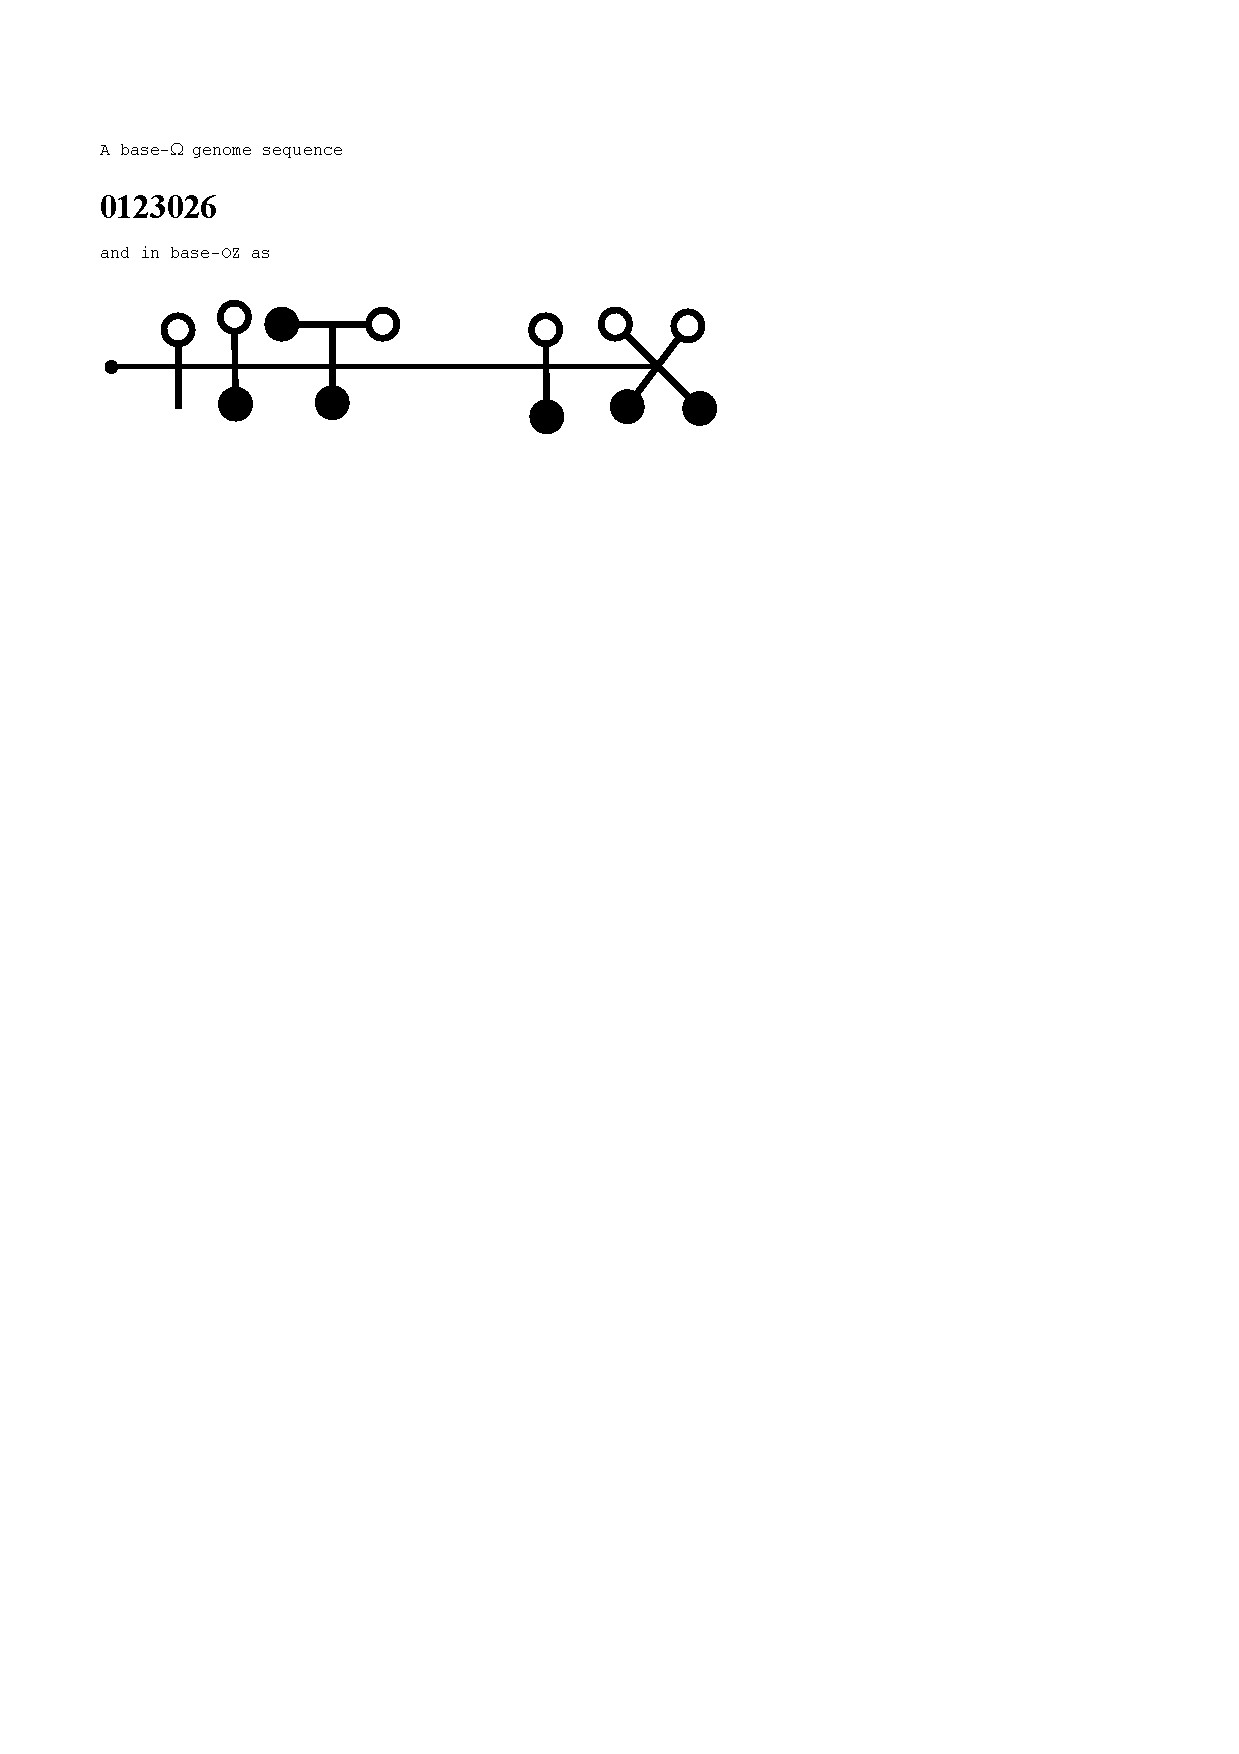
\includegraphics[trim=0cm 20cm 0cm 0cm, clip, width=0.9\textwidth,]{resources/pdfs/OZINCIPHER-APP3-EXA.pdf}\\
   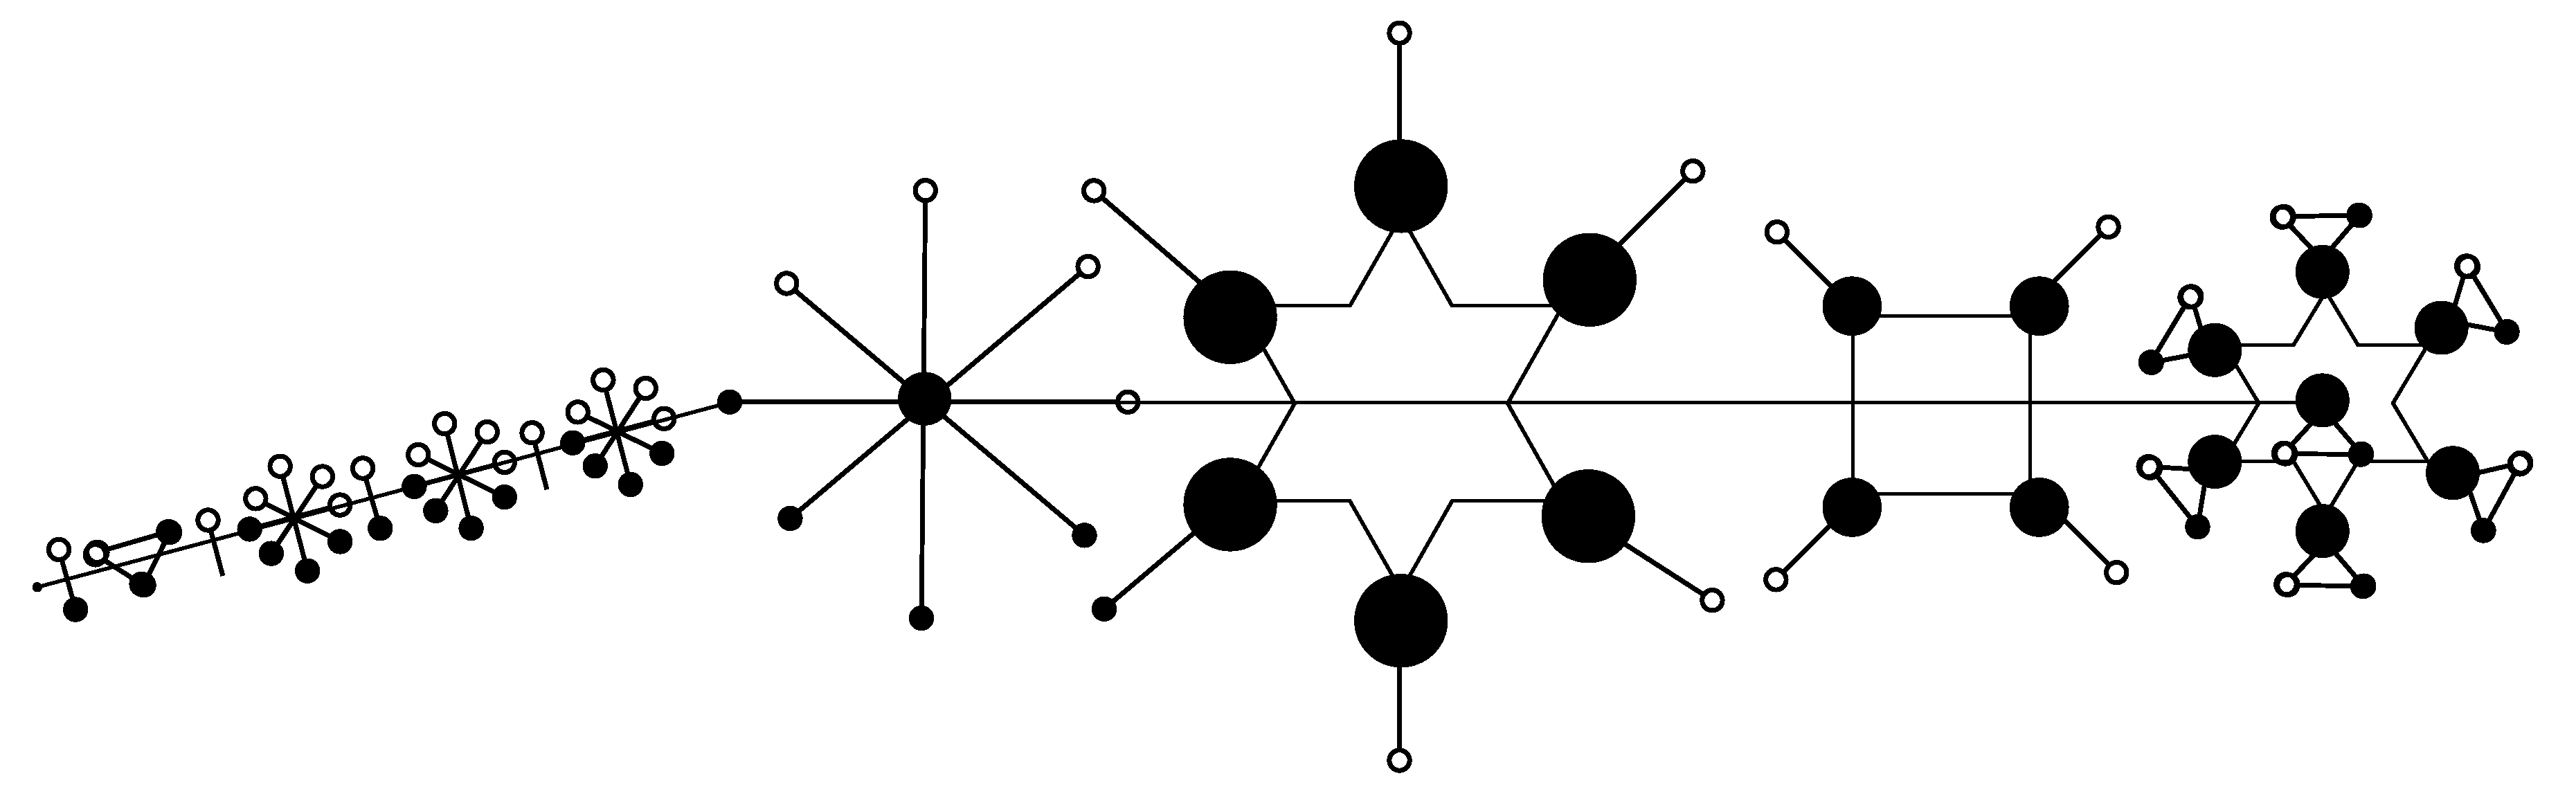
\includegraphics[trim=0cm 0cm 0cm 0cm, clip, width=0.9\textwidth,]{resources/pdfs/PLATONIC-EULERVIRUS-landscape.pdf}\\
      \caption{The equivalent LGES complete genome expression of the $\Omega_{veuler}$ (Euler Virus) genome sequence (from \textbf{\hyperref[EQGFEEVIRUS]{Equation \ref{EQGFEEVIRUS}}})}
  \label{FIGLGESEULERVIRUS}
  \end{center}
\end{figure}


Now, concerning that rendering of the genome sequence expressed in \textbf{\hyperref[EQGFEEVIRUS]{Equation \ref{EQGFEEVIRUS}}}, it might be worth noting that unlike the earlier examples of \textbf{LGES} expressions, we have taken the liberty to exploit that special joint that kick-starts the \textbf{PFA}, or rather, which separates the \textbf{IFA} from the \textbf{PFA} in a \textbf{FGE} expression. So, just like an organism with a physical joint might sometimes appear as angled or curved, so we have chosen to depict the $\Omega_{veuler}$ with its one joint\footnote{Definitely, and interesting to explore, a genome sequence with multiple JOINT points in it might be how an organism with say multiple appendages such as legs, hands and a head that can move independently of the core/thorax of the body is possibly arrived at. The interested student should go ahead and explore more non-trivial $\Omega$-base sequences just to see what's possible.} well utilized. However, and important to note; it is not just joints that might appear different across different renderings of the same basis genome sequence. So, in \textbf{\hyperref[FIGLGESEULERVIRUSv2]{Figure \ref{FIGLGESEULERVIRUSv2}}}, we see another rendering of the same genome sequence expression, with readily noticeable differences being the IFA-PFA joint in its neutral position (we also simplified and fused it with one of the edge-nodes of the $1_{pf} \otimes 8_{oz}$ term in both diagrams), and then the second term in the PFA (corresponding to \textbf{$7_{pf} \otimes 2_{oz}$} or rather \textbf{$7_{pf} + 7 \times 2_{oz}$}) with the $2_{oz}$ appendages depicted mostly aligned horizontally --- basically, there's still room for some creativity while rendering, but perhaps the future and more research might help decide on what is optimal/ideal. At the moment, it is mostly the mathematics, a sane dose of and principles of aesthetics and design, but also, trusting that in nature, systems are at their \textit{most basic form}, when in states of lowest kinetic energy or highest potential energy\footnote{Such as, not finding trees that grow with their stems at an angle to the ground or animals with curved legs or walking on 3 legs or with the legs all at the back --- for 4-legged animals, etc... Thus, though I didn't cite any authority on this matter (except perhaps nature), I trust that basic physics applied to anatomy and physiology might help justify the sensibilities we only seem to be applying from basic understanding of physics and nature here --- \textit{natural axioms} and \textit{instincts} perhaps.}.


\begin{figure}[H]
  \begin{center}
  %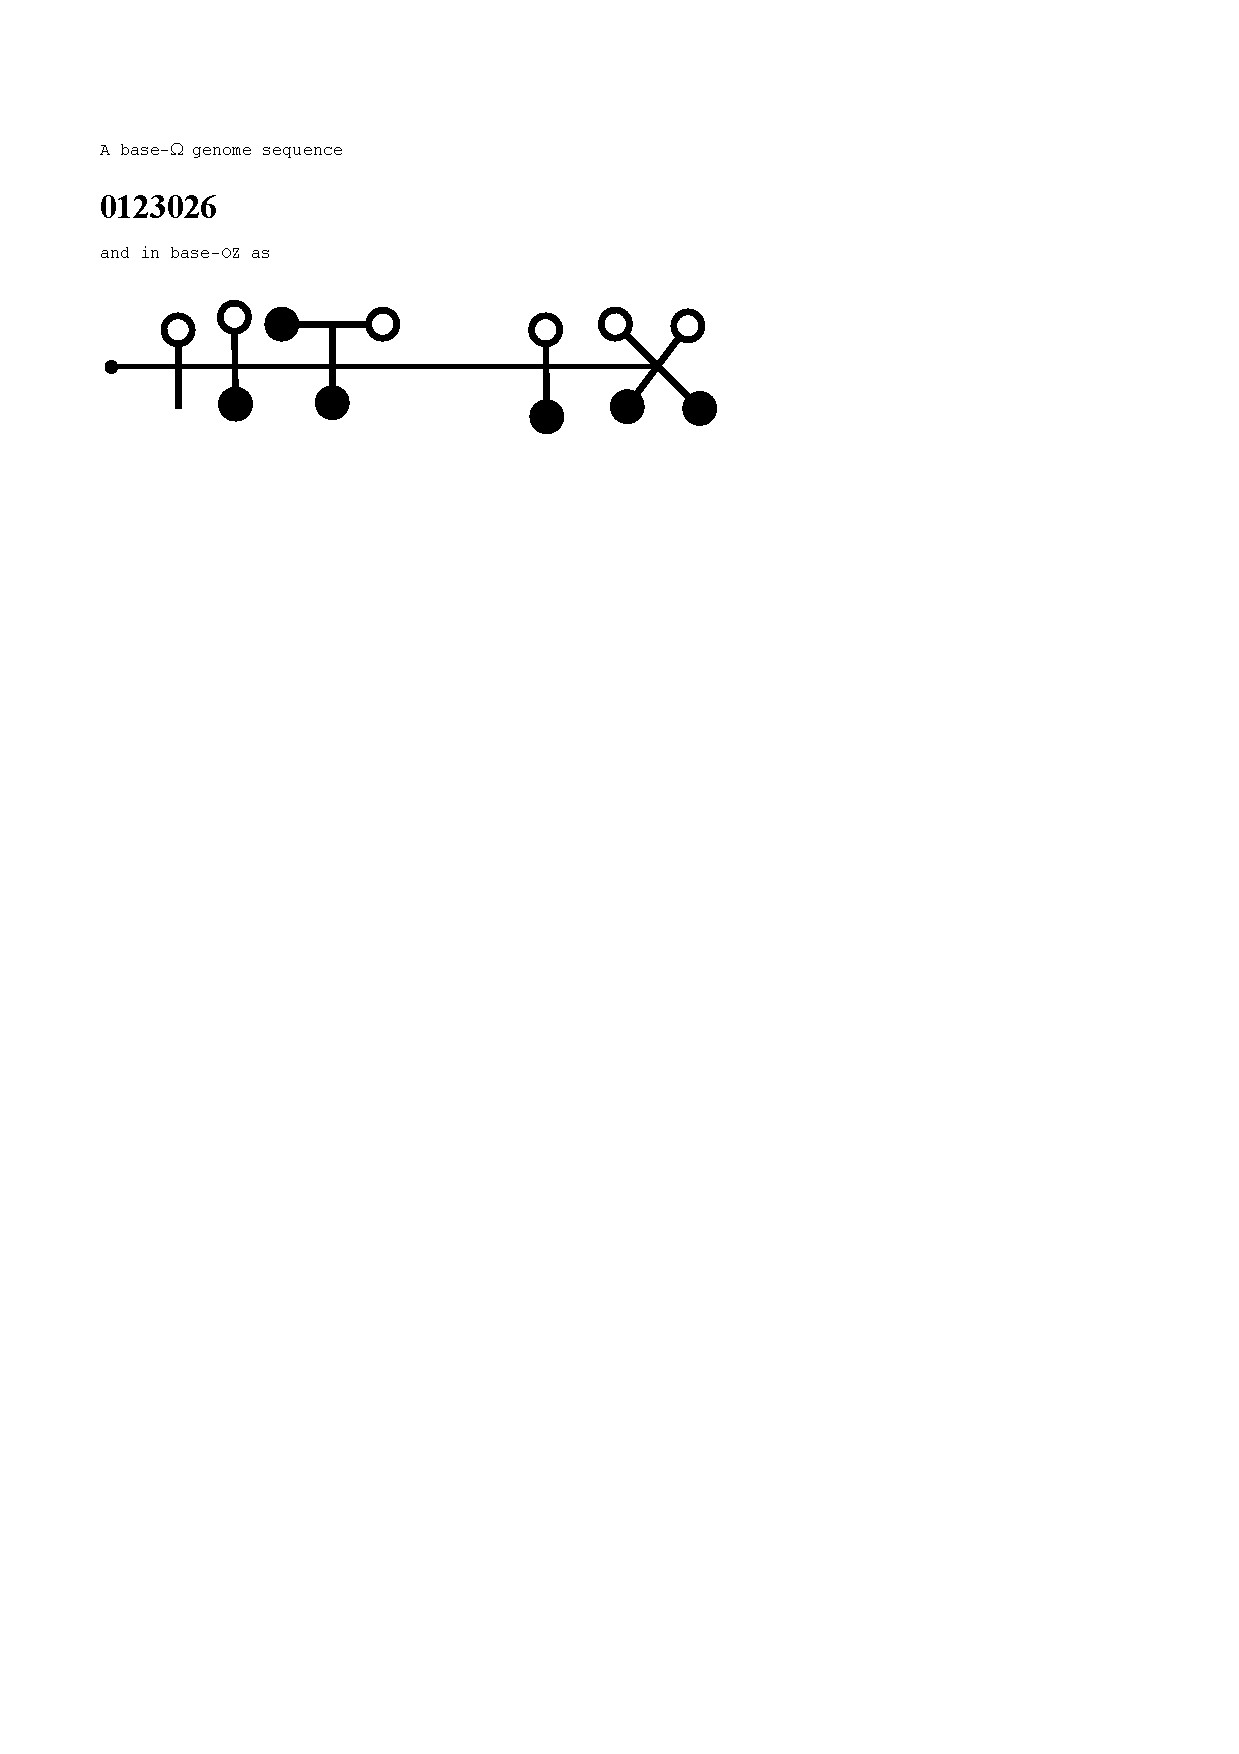
\includegraphics[trim=0cm 20cm 0cm 0cm, clip, width=0.9\textwidth,]{resources/pdfs/OZINCIPHER-APP3-EXA.pdf}\\
   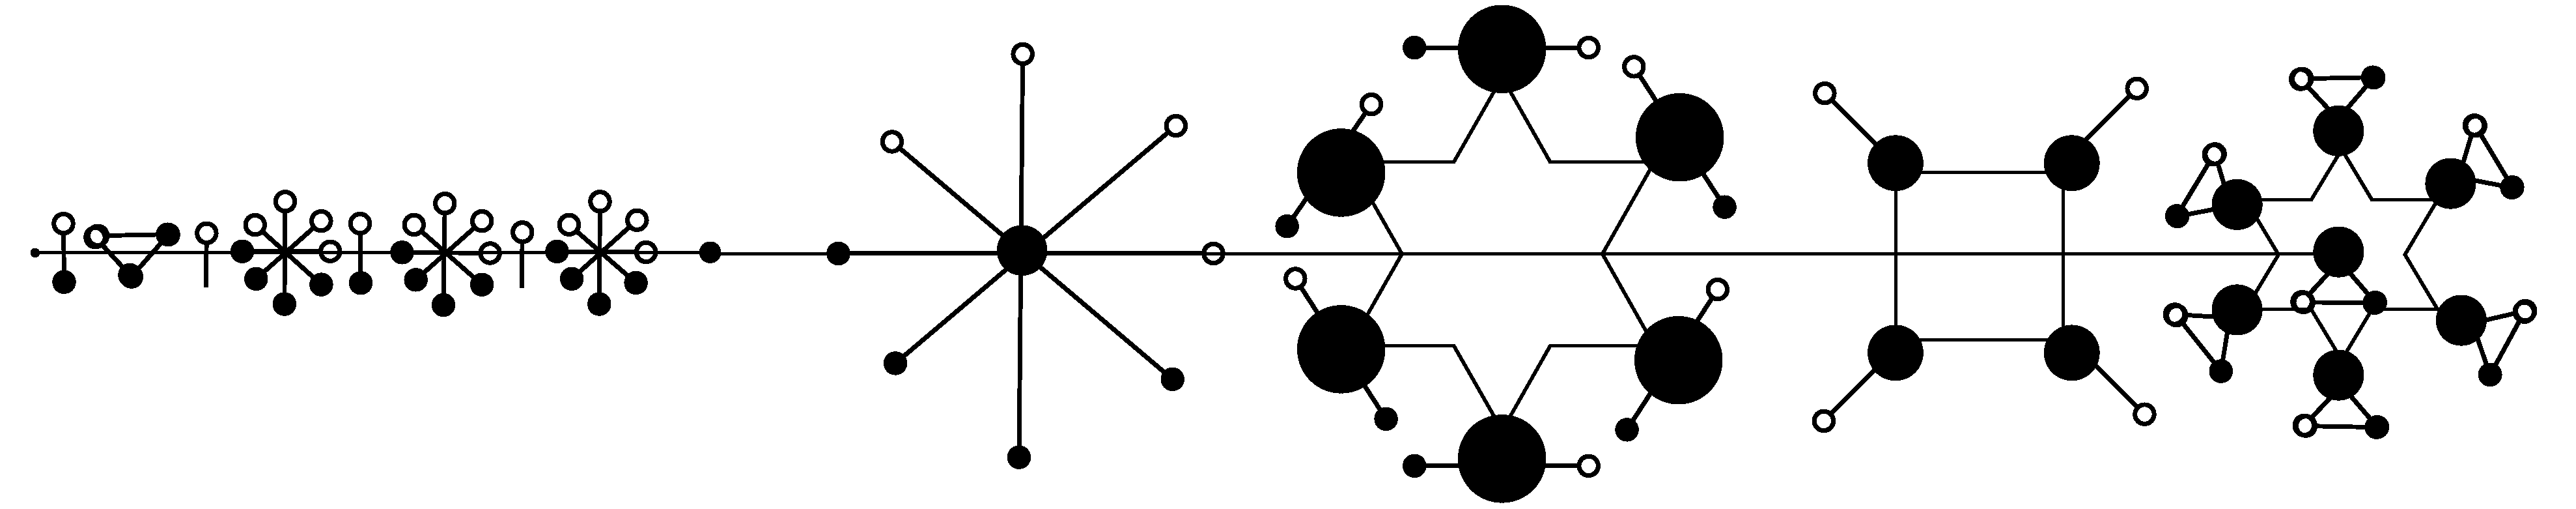
\includegraphics[trim=0cm 0cm 0cm 0cm, clip, width=0.9\textwidth,]{resources/pdfs/v2-PLATONIC-EULERVIRUS-landscape.pdf}\\
   \caption{An \textbf{alternative rendering} of the same sequence as $\Omega_{veuler}$ originally depicted as the \textbf{LGES} genome expression in \textbf{\hyperref[FIGLGESEULERVIRUS]{Figure \ref{FIGLGESEULERVIRUS}}}}
  \label{FIGLGESEULERVIRUSv2}
  \end{center}
\end{figure}

And talking of scaling nodes, in the future, we might want to explore whether in such a system as \textbf{LGES} in which the expression is sensitive to measures such as the \textbf{IFA MSS}, whether it might make sense to scale each subsequent pf-node in the \textbf{PFA} based on its position within the sequence? Though we didn't have such a rule included in \textbf{\hyperref[ALGCOZINPLATO]{Algorithm \ref{ALGCOZINPLATO}}}, and yet, our example renderings here have somewhat taken advantage of that plausible logic.

That said, note that, we started this work with a photograph of a pineapple ready to harvest (see \textbf{\hyperref[FIGPINEAPPLE]{Figure \ref{FIGPINEAPPLE}}}), and though the associated discussion\footnote{Checkout video/mini-lecture concerning this particular organism and what might be gleaned about genetic expressions from it, via author's YouTube Channel: \url{https://youtube.com/shorts/yTJzBEpw7Z4}} did bring up the matter of how it might inspire a genome expression system in which the prefix is the actual DNA that renders the rest of the organism (fruit, plant-base and roots in this case of the pineapple), it is left as an exercise to the reader, to decide whether example genome sequence expressions/renderings such as in \textbf{Figure \ref{FIGLGESEULERVIRUS}} depict this pineapple-inspired philosophy.


\begin{center}
\fbox{\begin{minipage}{0.9\textwidth}
\large
\textbf{NOTE:}\\
 On \textbf{Why Place-Notation Expression Systems Matter} \\

As a further justification for why we chose to use a place-notation sensitive genetic code expression system in our conceptual genome expression thought experiment, consider that, just like with modern numbers and number sysems --- of which the Arabic number system is considered one of the best since ancient times, the occurrence of a symbol within an expression is interpreted not just by what it quantifies, but also by where in the expression it is situated. 

For good measure, a few enlightening quotes from the priceless work on the evolution of number systems since ancient times, by Raymond S. Nickerson, shall help cement this ideology:

\begin{quotation}
\noindent \texttt{Aristotle attached considerable significance to the fact that human beings can count: it is this ability, he claimed, that demonstrates our rationality.}\\\\

\noindent \texttt{As Brainerd (1973) has pointed out, in most Western nations today we expect students, by the time they reach their early teens, to be much more competent with numbers than was an educated adult Greek or Roman of 2,000 years ago. This fact arises in no small measure from the elegance and power of the scheme that we now use to represent numbers.}\\\\


\noindent \texttt{In short, a price of the increased abstractness of the Arabic system is an obscuring of some of the key principles on which numbers are based. To an ancient Egyptian, the fact that 3+4=7 was apparent from the relationship between the Egyptian number representing 7 and those representing 3 and 4. There is no hint of such a relationship, however, when this equation is expressed in Arabic notation. The price has been worth the paying, however.}\\\\


\noindent \texttt{If you invented a unique symbol to represent each of the possible quantities of stones (including the case of no stones) up to that of your standard and decided to use the position of that symbol to indicate the pile to which it refers, you would have what we refer to today as a place-notation system for representing numbers.}\\\\

\noindent \texttt{The relative ease with which one can count or compute depends to no small degree on the characteristics of the system that is used to represent number concepts.}\\

\hspace*{\fill} ---\textbf{Raymond S. Nickerson}, \textit{Counting, Computing, and the Representation of Numbers}, 1988\cite{nickerson1988counting}
\end{quotation}

And finally, it shall be worth noting that this notion also underlies the present author's use of the \textbf{Position-Index measure} ($I(\omega_i, \Theta)$), first formalized in the Base-36 paper\cite{base36paper}, and which, among many important applications it has, is its use in generalizing the computation of decimal values of arbitrary number expressions in any base, its use in transformatics to express sequence summaries using modal sequences\cite{transformatics}, etc.

\end{minipage}}
\\
\end{center}


\section{The Extended Lu-Genome Expression System (x-LGES)}
\label{SECxLGES}

If you look at the genome sequence expressions that we have encountered in \textbf{\hyperref[SECFULLGES]{Section \ref{SECFULLGES}}}, and compare that to the case of our pineapple in \textbf{\hyperref[FIGPINEAPPLE]{Figure \ref{FIGPINEAPPLE}}} that opens the introductory chapter, you shall notice that, just in case we assume our \textbf{LGES} protocols to be sufficient for the expression of not just bits of an organism, but also relevant to the expression of \textbf{the complete organism}, then, it might seem like something is still missing, and thus the \textbf{Extended Lu-Genome Expression System} (x-LGES).


So, what exactly is missing from our genome expressions thus far? We shall call out a few telling points to help drive the point home:

\begin{enumerate}
\item As has been stressed already, and as is the case that we wish our science to not be constructed in ivory towers alienated from facts and reality in nature, we must borrow a leaf from how actual DNA is utilized to express organisms in reality. For example, it is not that one genome expresses the hands, another the heart, and yet another the eyes! Well, of course, in a particular organism's DNA, there shall be specific subsequences that best define the expression of particular features or aspects of an organism, however, overall, a single, complete genome sequence is and should be sufficient for the complete expression of an entire organism with all its various attributes and distinct aspects well catered for.
\item When we consider the way the original \textbf{LGES} algorithm is specified\footnote{Not to be confused with \textbf{\hyperref[ALGCOZINPLATO_ORIG]{Algorithm \ref{ALGCOZINPLATO_ORIG}}} (now in the \textbf{Appendix}: \textbf{\hyperref[SECALTPFGESA]{Chapter \ref{SECALTPFGESA}}}).} --- \textbf{\hyperref[ALGCOZINPLATO]{Algorithm \ref{ALGCOZINPLATO}}}  being the one that combines both transcription and translation into a single process, we shall note that, the final output of that process --- as depicted in \textbf{\hyperref[EQTRANSLGENSEQ]{Equation \ref{EQTRANSLGENSEQ}}} for the general case, and as in \textbf{\hyperref[EQGFEEVIRUS]{Equation \ref{EQGFEEVIRUS}}} for one particular organism's expression (in \textit{numerical form}), we notice that, especially when approached from the point of view of the fully-processed rendering of the \textbf{FGE}, $\boxed{OZ(\Theta_\Omega)}^*$, some potentially relevant information could be considered to be \textit{missing}\footnote{Well, technically, unless when one is only studying the visual expressions corresponding to a particular genome sequence --- which might introduce a lot of variations and exploit a lot of creative freedom, when we instead express the genome in the mathematical form as in \textbf{\hyperref[EQGFEEVIRUS]{Equation \ref{EQGFEEVIRUS}}}, almost all the necessary information about the genome is present at that moment, including the important statistical summary information from the \textbf{IFA MSS}.} from that expression at that point. In particular, when we have the \textbf{PFA} expressed in its platonic form, it might not readily be possible to discern the vital $\overset{>}{OZ(\Theta_\Omega)}$ aspect since the actual \textbf{PFA} is a combination (see \textbf{\hyperref[EQFBOXED]{Equation \ref{EQFBOXED}}}) of that \textbf{IFA MSS} in its OZIN form as well as its translation into complementary Platonic Form expressions via the \textbf{\hyperref[FIGPLATONICCIPH]{PLATO CIPHER}}.
\item Finally, and again, returning to nature as our authority on genome expression, we note that, most organisms --- plants or animals, typically manifest in a \textbf{PREFIX-THORAX-SUFFIX}/\textbf{HEAD-BODY-ROOT} form. Looking at our \textbf{LGES} renderings in \textbf{\hyperref[SECFULLGES]{Section \ref{SECFULLGES}}}, we see that the \textbf{IFA} aspect properly caters for the ``PREFIX/HEAD" component --- it somewhat contains the entire [genome] sequence just encoded in base-OZ\footnote{Interesting to say, ``the brains" of the expressed organism, especially since it has the complete genome almost unaltered, and in its \textit{actionable form}.}. Then we have the ``THORAX/BODY" bit. It feels plausible to equate that with the protracted spatial-expressions of the \textbf{PFA}. But what of the ``SUFFIX/ROOT" component? And talking of suffixes in natural genome expressions; we can appreciate that for humans, birds and most animals, we can talk of \textbf{legs}; for aquatic animals especially, such as fish, we might talk of \textbf{tail-fins}; for insects and all various kinds of arthropods, we can not only talk of a body form that's generally made up of chained bits or adjoined segments such as in our \textbf{LGES}, but that they generally terminate in a kind of suffix we might consider to be \textbf{an abdomen}. And then finally, for plants, it's obvious they typically terminate in \textbf{roots} --- and especially for the case of food-crops, we find that these roots contain sufficient \textit{bio-information} to allow us to reproduce the original plant organism from just those suffixes\footnote{Though not all root-crops might readily be grown from their root tubers, some good examples from observation and experience author has obtained practicing domestic crop-husbandry include irish potatoes (\textit{obutakuli}), yams (\textit{ebihuna}), onions (\textit{obutunguru}), ginger (\textit{entangahuzi}) and (\textit{binyobwa}) ground-nuts! And talking of which, for the aspect of being able to re-grow an organism from its affixes --- head/prefix or root/suffix, the interesting case of the sweet-potato, would be a fun case; despite being a root-crop as those mentioned before, attempts to re-grow it say by reburying a sweet-potato tuber, is so futile! Only way is to take the leaves (prefixes) and partially-bury them in soil, so as to re-grow the complete sweet-potato plant!}.
\end{enumerate}

So, with those observations and criticisms of the original \textbf{LGES}, we can provide a solution in form of the following algorithm that extends \textbf{\hyperref[ALGCOZINPLATO]{Algorithm \ref{ALGCOZINPLATO}}}:


\subsection{$\psi_{\Omega}$-to-($\psi_{oz}$-$\psi_{pf}$-$\psi_{oz}$): The x-LGES Algorithm}
\label{SECGENSEQEXPRESEXT}


To render a complete genome expression using this extended algorithm, and starting from the original genome sequence encoded as a base-$\Omega$ expression, we proceed as such: 

\begin{alg}[The \textbf{x-LGES Algorithm}]
\label{ALGCOZINPLATOEXT}

Assuming we have an $\Omega$-base encoded genetic code sequence $\Theta_\Omega$ of some length $n > 0$.

\begin{enumerate}
\item{\textbf{INITIALIZE} the final expression by constructing the initial part of the \textbf{FGE} using \textbf{\hyperref[ALGCOZINPLATO]{Algorithm \ref{ALGCOZINPLATO}}} to construct the \textbf{Intermediate Form Affix} (IFA) of $\Theta_\Omega$ \textbf{and} the \textbf{Platonic Form Aspect (PFA)} --- so that at this point, the complete expressed(transcribed+translated) sequence shall be as:\\

\begin{equation}
\label{EQTRANSLGENSEQEXT}
\boxed{OZ(\Theta_\Omega)}^* = OZ(\Theta_\Omega)\cdot\boxed{OZ(\Theta_\Omega)}
\end{equation}\\

}
\item {
\textbf{EXTEND} that initial \textbf{FGE} with just \textbf{a single GAP/JOINT extension}, so that we then have the \textbf{FGE} as such:

		\begin{equation}
		\label{EQEXTFGEJOINTEXT}
		\boxed{OZ(\Theta_\Omega)}^* = \boxed{OZ(\Theta_\Omega)}^* \cdot \boxed{\omega_i^*}_{joint}
		\end{equation}		
		
		And equivalently:
		
		\begin{equation}
		\label{EQEXTFGEJOINTSUFEXT}
		\boxed{OZ(\Theta_\Omega)}^* = OZ(\Theta_\Omega)\cdot\boxed{OZ(\Theta_\Omega)} \cdot \boxed{\omega_i^*}_{joint}
		\end{equation}				

}
\item {

Then, \textbf{USE} the \textbf{IFA MSS} from \textbf{Step\#1}/\textbf{\hyperref[ALGCOZINPLATO]{Algorithm \ref{ALGCOZINPLATO}}}, that is $\overset{>}{OZ(\Theta_\Omega)}$, as the \textbf{Genome Expression Suffix (GES)} to extend the current \textbf{FGE} so that

\begin{equation}
\label{EQTRANSLGENSEQEXT}
\boxed{OZ(\Theta_\Omega)}^* = OZ(\Theta_\Omega)\cdot\boxed{OZ(\Theta_\Omega)}\cdot\overset{>}{OZ(\Theta_\Omega)}
\end{equation}\\

Which, if qualified with the necessary encoding bases is as such:

\begin{equation}
\label{EQTRANSLGENSEQEXTQUAL}
\boxed{OZ(\Theta_\Omega)}^* = OZ(\Theta_\Omega)_{oz}\cdot\boxed{OZ(\Theta_\Omega)}_{pf}\cdot\overset{>}{OZ(\Theta_\Omega)}_{oz}
\end{equation}

And if we express this as the update to \textbf{\hyperref[EQEXTFGEJOINTEXT]{Equation \ref{EQEXTFGEJOINTEXT}}}, we have:

\begin{equation}
		\label{EQEXTFGEJOINTEXT_B}
		\boxed{OZ(\Theta_\Omega)}^* = \boxed{OZ(\Theta_\Omega)}^* \cdot \boxed{\omega_i^*}_{joint} \cdot\overset{>}{OZ(\Theta_\Omega)}_{oz}
		\end{equation}	
		
		Which tells us that the final \textbf{FGE} is the original \textbf{FGE} extended with just one extra JOINT and the \textbf{GES}/\textbf{IFA MSS} encoded in base-OZIN.

}
\item \textbf{TRUNCATE} the final-structure after the final term in \textbf{FGE}.
\item \textbf{RETURN} that final \textbf{FGE}, $\boxed{OZ(\Theta_\Omega)}^*$, as the final transcribed and translated version of $\Theta_\Omega$. The culmination of our extended genome expression system.
\end{enumerate}
\end{alg}


We shall come to appreciate this updated protocol in \textbf{\hyperref[ALGCOZINPLATOEXT]{Algorithm \ref{ALGCOZINPLATOEXT}}}, by taking a few of the \textbf{FGE} examples we looked at earlier, and re-render them using the \textbf{x-LGES} to see what difference it makes.



\begin{figure}[H]
  \begin{center}
  %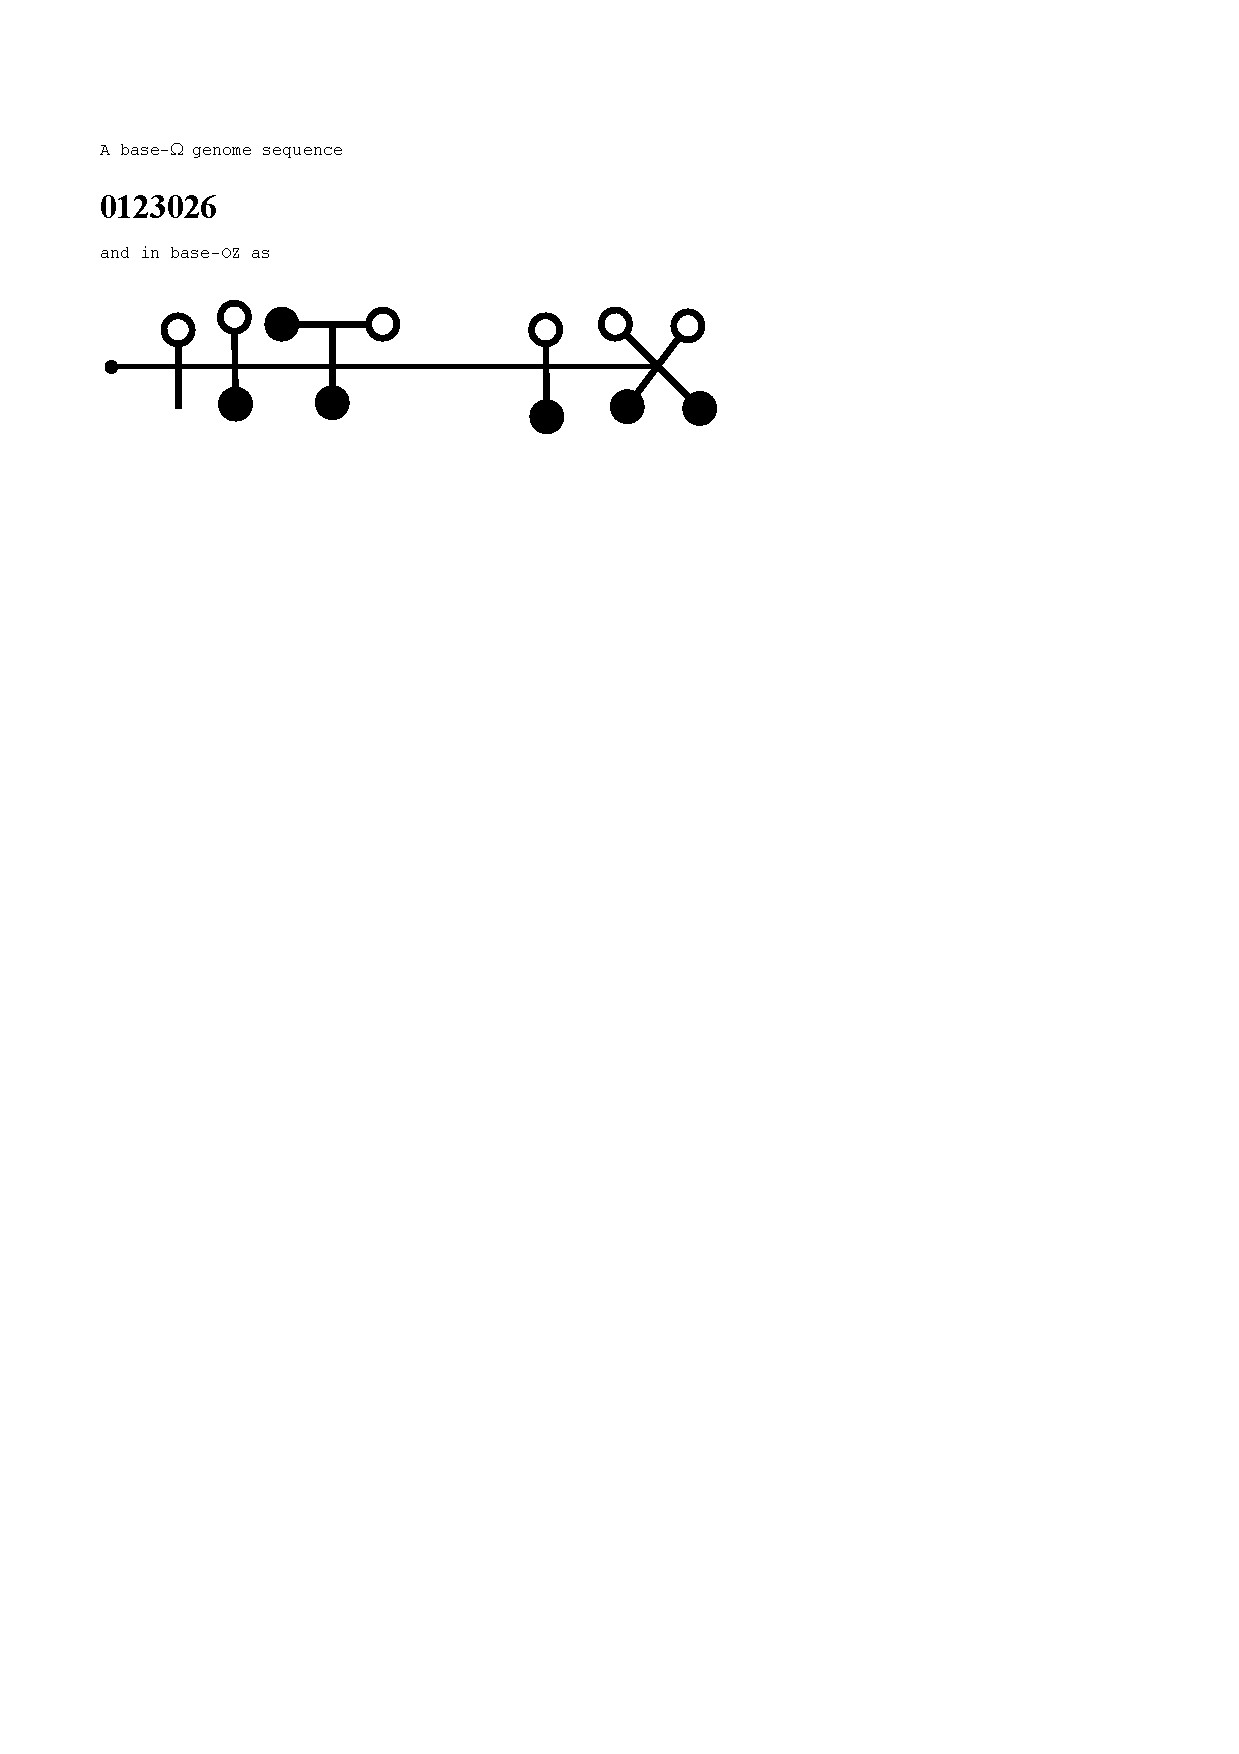
\includegraphics[trim=0cm 20cm 0cm 0cm, clip, width=0.9\textwidth,]{resources/pdfs/OZINCIPHER-APP3-EXA.pdf}\\
   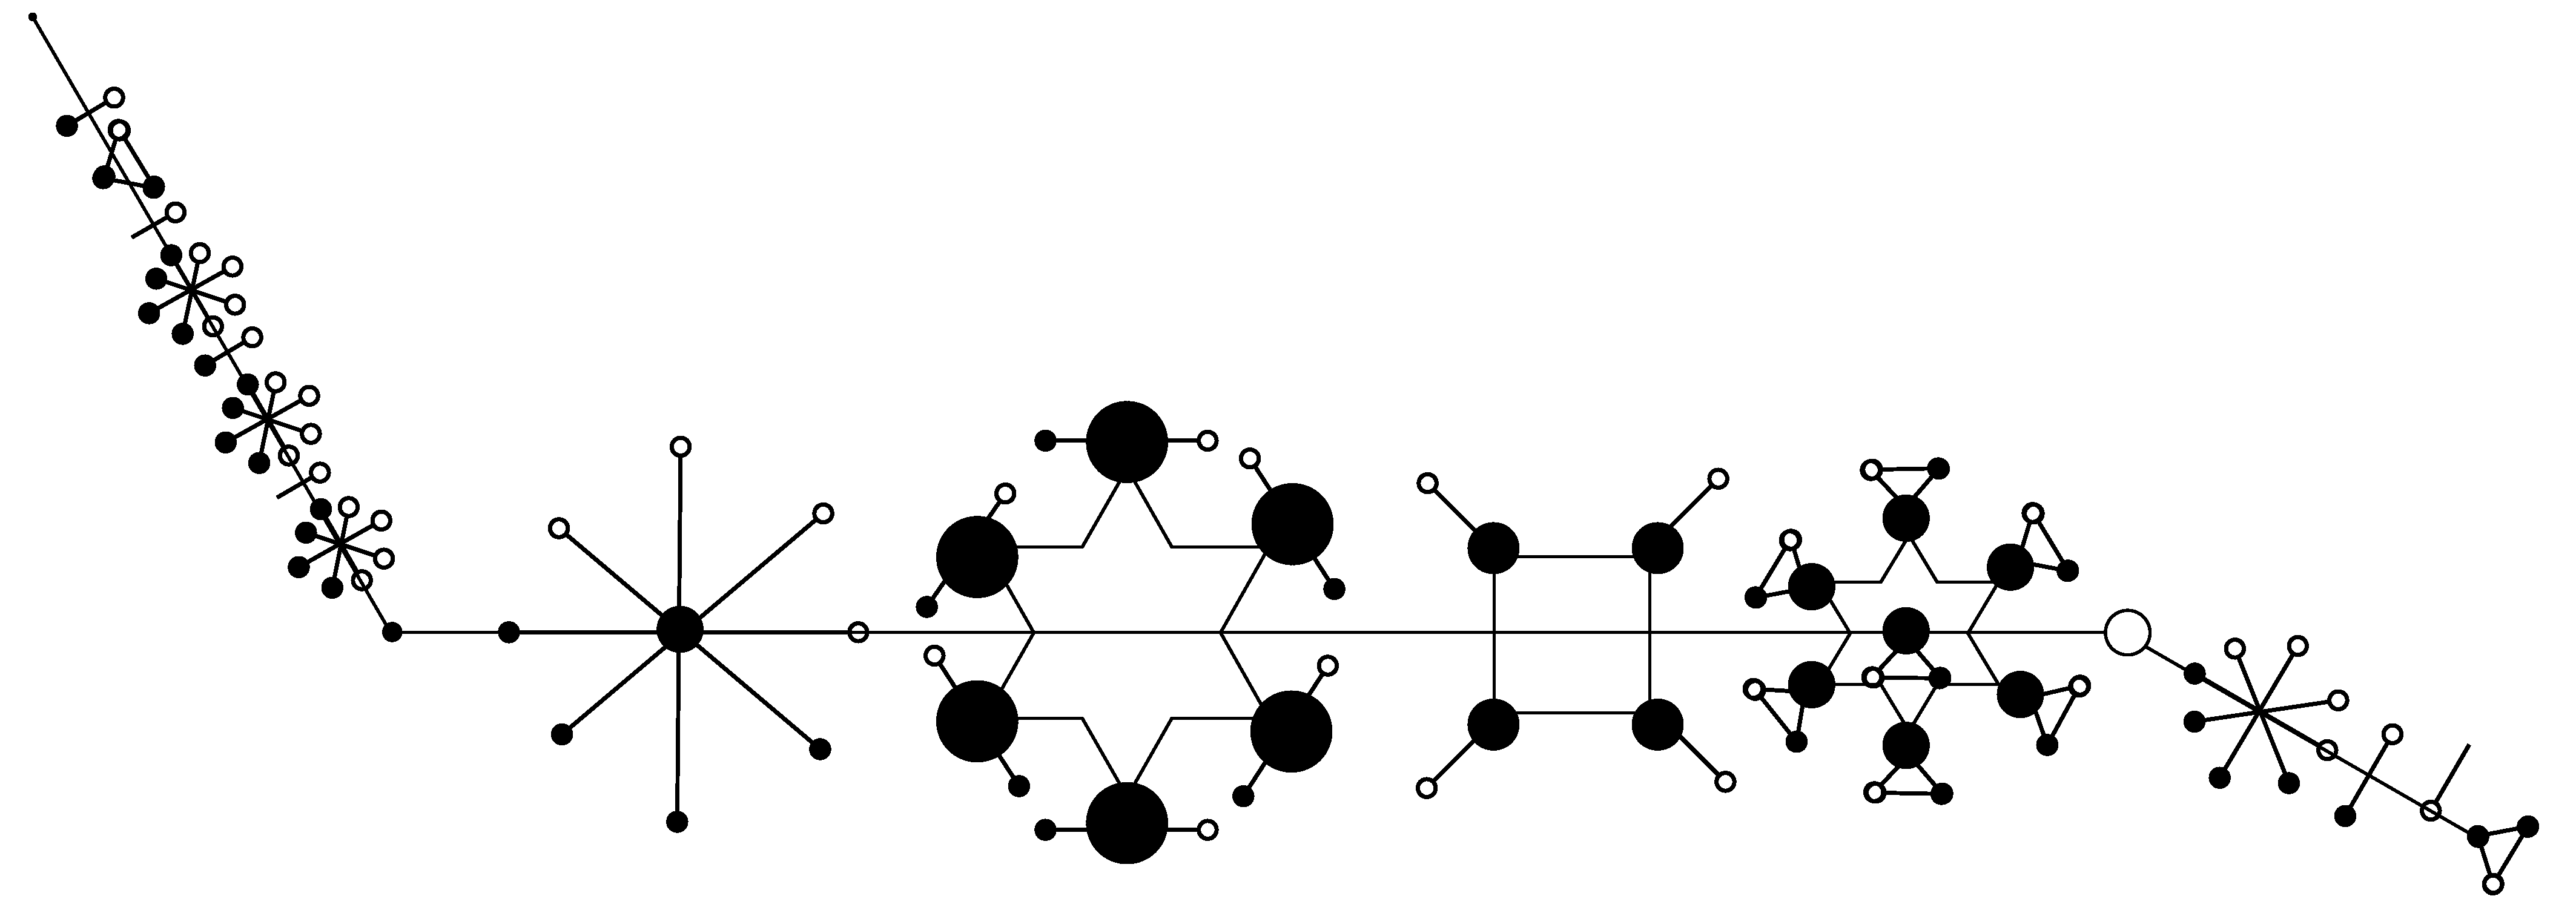
\includegraphics[trim=0cm 0cm 0cm 0cm, clip, width=0.9\textwidth,]{resources/pdfs/EXT-v2-PLATONIC-EULERVIRUS-landscape.pdf}\\
   \caption{The \textbf{x-LGES form rendering} of the $\Omega_{veuler}$, the \textbf{Euler Virus}, now with HEAD, BODY and ROOT segments.}
  \label{FIGLGESEULERVIRUSv2EXT}
  \end{center}
\end{figure}

The first example is with the notorious \textbf{Euler Virus} originally defined in \textbf{\hyperref[EQDNAV]{Equation \ref{EQDNAV}}}, and this rendering shown in \textbf{\hyperref[FIGLGESEULERVIRUSv2EXT]{Figure \ref{FIGLGESEULERVIRUSv2EXT}}} shall start to paint the new picture for you, if you compare it to the original OZIN-expression of its equivalent \textbf{mRNA} as shown in \textbf{\hyperref[FIGOZEVIRUS]{Figure \ref{FIGOZEVIRUS}}}, and then, that same organism as the basic \textbf{LGES}-form in \textbf{\hyperref[FIGLGESEULERVIRUSv2]{Figure \ref{FIGLGESEULERVIRUSv2}}} which shows the full genome expression minus the extension \textbf{GES} SUFFIX/ROOT.


\section{Actual DNA Sequences Expressed in the Extended Lu-Genome Expression System}

So, now that we have finished looking at what could happen with genome expression under the hypothetical LGES protocols, one might wonder, and correctly so, how might we use that system to attempt to visualize actual na-Sequences such as DNA or RNA sequences or subsequences?


\vspace{2em}
\fbox{
\begin{minipage}{0.9\textwidth}
\textbf{On Barriers to Entry:}\\

Concerning working with the \textbf{LGES} or \textbf{x-LGES} as it is at the moment, the entry point barrier is that the system is defined for sequences expressed in base-10 only. That means, unless your sequence is expressed using symbols from $\psi_{10}$, there is no direct way to leverage the theory we have just presented. So, that's where we need put our attention first, with regards to processing DNA or RNA in this thought experiment --- and for any other kinds of sequences one might wish/attempt to visually express using our system.

\end{minipage}}
\\
\vspace{2em}


Good enough, we have had extensive background concerning transformation of sequences across symbol sets in earlier chapters and works by the author\cite{base36paper}\cite{lnspaper}\footnote{Also see \cite{bosse2025repeating}.}, and so, we can just re-iterate some points here.

\begin{itemize}
\item We know that any na-Sequence shall span $\psi_{na}$, which has cardinality 5 (refer to \textbf{\hyperref[LAWNA]{Law \ref{LAWNA}}}), and yet, $\invpi(\psi_{10}) = 10 > \invpi(\psi_{na})$.
\item For either DNA ($\psi_{DNA}$) or RNA ($\psi_{RNA}$), their corresponding symbol set cardinalities are just \textbf{4} and \textbf{4} respectively, which still doesn't map well to the base-10 or rather $\psi_{10}$ symbol set that the Lu-Genome Expression System requires.
\end{itemize}

So, using sequences we have already encountered, such as $\Theta_4^*$ in \textbf{\hyperref[EQ6B]{Equation \ref{EQ6B}}} --- an RNA sequence, or its original DNA form (as in \textbf{\hyperref[EQ5]{Equation \ref{EQ5}}}) how, should we go about expressing it in equivalent or sufficient $\Omega$-form?

\subsection{Converting Between Nucleic Acid Code and Numeric Codes}

First, given the constraints we have seen above, one plausible solution might be to start with a naive\footnote{I think it is naive, because, using the position-index operator $I(\omega,\Theta)$ in the encoding definition, it isn't clear how we shall ever resolve for the digit `0' given DNA has only 4 distinct symbols.} encoding that merely maps every element in $\psi_{DNA}$ to a corresponding term in $\psi_{10}$ \textbf{based not on the quantity of the symbol --- since na-Sequences aren't made of `literal numbers', but rather, based on the position of the symbol within the DNA symbol set}. So that, we have the following basic encoding-transformer:\\


\begin{transf}[$\psi_{DNA}$ to $\psi_{10}$ \textbf{DNA-Decimal Encoder}]
\label{TRANSFDNADECEN}
$ $\\
$\Theta \xrightarrow{O_{dna-dec-encode}(\cdot)} \Theta^*; \quad \forall \omega \in \Theta: I(\omega,\Theta) = k, \exists \rho \in \Theta^*: I(\rho,\Theta^*) = k \implies \rho = I(\omega,\psi_{DNA})$\\
\end{transf}


And so, using that \textbf{\hyperref[TRANSFDNADECEN]{Transformer \ref{TRANSFDNADECEN}}}, we can process any DNA sequence and map it to corresponding $\Omega$-form (or rather \textit{decimal form}) as such:

\[
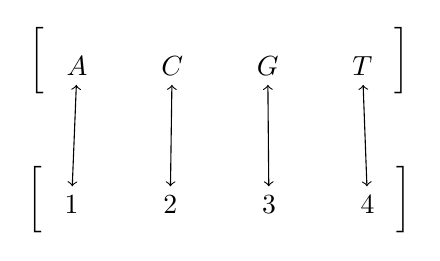
\begin{tikzpicture}[baseline=(current bounding box.center)]
  % Matrix A
  \matrix (A) [matrix of math nodes, left delimiter={[}, right delimiter={]}, row sep=1em, column sep=2em] {
    A & C & G & T \\
  };

  % Matrix B
  \matrix (B) [matrix of math nodes, left delimiter={[}, right delimiter={]}, row sep=1em, column sep=2.4em, below=3em of A] {
    1 & 2 & 3 & 4 \\
  };

  % Draw arrows from A_i to B_i
  \foreach \i in {1,2,3, 4}
    \draw[<->] (A-1-\i) -- (B-1-\i);
\end{tikzpicture}
\]


With that basic mapping, and our example DNA sequence from \textbf{\hyperref[EQ5]{Equation \ref{EQ5}}}) we see that the corresponding decimal-encoded DNA sequence shall merely be as in the following transformation:

\begin{trans}
\label{TRANSSEQATG}
$\Theta = \langle  A, T, G, A, A, A, T, T, A, T, A, G \rangle$\\
$ \xrightarrow{O_{dna-dec-encode}(\cdot)} \langle  1, 4, 3, 1, 1, 1, 4, 4, 1, 4, 1, 3 \rangle$
\end{trans}

Essentially, the symbol set for DNA sequences encoded in decimal shall only span the special symbol set we might refer to as \textbf{DNA-Digits Symbol Set}, and which we might denote as $\psi_{DD}$, and which is just:\\


\begin{equation}
\label{EQDNADIGSS}
\psi_{DD} = \langle 1, 2, 3, 4 \rangle
\end{equation}\\


So, with $\psi_{DD}$ and knowing the mapping from DNA to Decimal, we could also work backwards from decimal sequences back into DNA sequences. So, for example, assuming we took the interesting \textbf{Hi-Fi o-SSI} from \textbf{\hyperref[EQDNHIFI]{Equation \ref{EQDNHIFI}}}, and wanted to map it to an equivalent DNA sequence, we might proceed by combining the consequences of \textbf{\hyperref[THEOCOMPEQUIV]{Theorem \ref{THEOCOMPEQUIV}}} and  \textbf{\hyperref[TRANSFDNADECEN]{Transformer \ref{TRANSFDNADECEN}}}. Thus, we might start by resolving to the following approximate numerical sequence:\\


\begin{trans}
\label{EQDNHIFINUM}
$ $\\
$\Omega_{HiFinelle} = \langle 8,6,4,9,1,3,7,5,2,0 \rangle \rightarrow  \langle 8,6,T,9,A,G,7,5,C,0 \rangle $\\
\end{trans}




However, as warned earlier on, transformations via \textbf{\hyperref[TRANSFDNADECEN]{Transformer \ref{TRANSFDNADECEN}}} would be somewhat \textit{weak} when dealing with the reverse case --- decimal-to-DNA decoding, especially because not all symbols in $\psi_{10}$ shall have meaningful equivalent terms in $\psi_{DNA}$. So, better we start by solving that problem instead.

Thus, with some \textit{necessary tweak} --- that, instead of mapping from $\psi_{DNA}$ to $\psi_{10}$ and vice-versa, we take $\psi_{na}$ which has exactly 5 elements and which is a superset of $\psi_{DNA}$\footnote{Refer to \textbf{\hyperref[DEFNASEQ]{Definition \ref{DEFNASEQ}}}}, and then map any symbol from $\psi_{na}$ to $\psi_{10}$ and vice-versa as per the following non-trivial transformer:


\begin{center}
\fbox{
\begin{minipage}{\textwidth}
\begin{transf}[$\psi_{na}$ to $\psi_{10}$ \textbf{na-to-Decimal Decoder}]
\label{TRANSFDECTONASEQ}
$ $\\
$\Theta \xrightarrow{O_{na-dec-decode}(\cdot)} \Theta^*;$\\
$\forall \omega_i \in \psi_{na}: I(\omega_i,\psi_{na}) = i \implies \exists d_j \in \psi_{10}: I(d_j,\psi_{10}) = j = i \quad \lor \quad I(d_j,\psi_{10}) = \invpi(\psi_{na}) + i \quad \implies \omega_i \leftrightarrow d_j $\\
$\land \quad \forall \alpha_k \in \Theta \quad \exists d_k \in \Theta^*: I(\alpha_k,\Theta) = I(d_k,\Theta^*) = k \quad \land \quad I(d_k,\psi_{10}) = I(\alpha_k,\psi_{na}) \lor I(d_k,\psi_{10}) = \invpi(\psi_{na}) + I(\alpha_k,\psi_{na}) \quad \implies \alpha_k \leftrightarrow d_k $
$\qed$\\
\end{transf}
\end{minipage}}
\\
\end{center}




So that, by \textbf{\hyperref[TRANSFDECTONASEQ]{Transformer \ref{TRANSFDECTONASEQ}}}, we arrive at complete decimal-to-DNA and decimal-to-RNA or generally decimal-to-na-Sequence symbol encoding-decoding is as shown in the following diagram:


\[
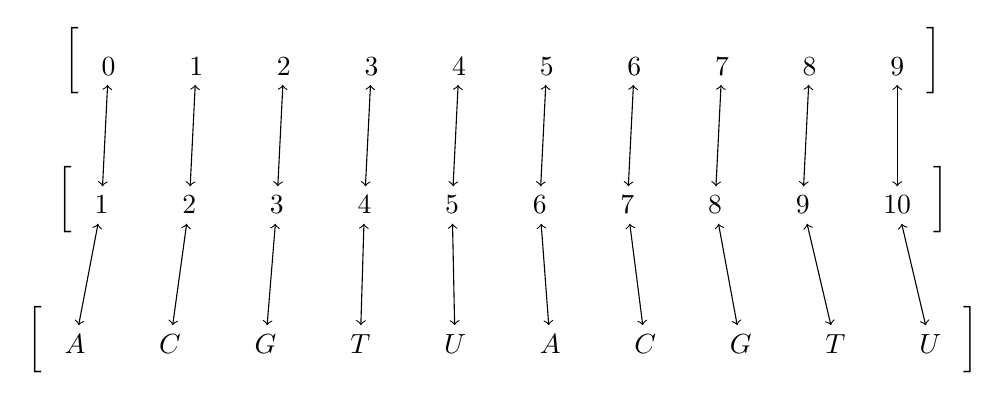
\begin{tikzpicture}[baseline=(current bounding box.center)]
  % Matrix A
  \matrix (A) [matrix of math nodes, left delimiter={[}, right delimiter={]}, row sep=1em, column sep=2em] {
    0 & 1 & 2 & 3 & 4 & 5 & 6 & 7 & 8 & 9\\
  };

  % Matrix B
  \matrix (B) [matrix of math nodes, left delimiter={[}, right delimiter={]}, row sep=1em, column sep=2em, below=3em of A] {
    1 & 2 & 3 & 4 & 5 & 6 & 7 & 8 & 9 & 10\\
  };
  
   % Matrix C
  \matrix (C) [matrix of math nodes, left delimiter={[}, right delimiter={]}, row sep=1em, column sep=2em, below=3em of B] {
    A & C & G & T & U & A & C & G & T & U\\
  };

  % Draw arrows from A_i to B_i
  \foreach \i in {1,2,3,4,5,6,7,8,9,10}
    \draw[<->] (A-1-\i) -- (B-1-\i);
    
  % Draw arrows from B_i to C_i
  \foreach \i in {1,2,3,4,5,6,7,8,9,10}
    \draw[<->] (B-1-\i) -- (C-1-\i);
\end{tikzpicture}
\]

Of course, the necessary tweak here, especially for target sequences specific to either DNA or RNA and not both, the tricky terms `T' and `U' need to be dealt with as necessary --- possibly with a basic swapping of all `U' with `T' for an na-Sequence targeting a DNA processor, and vice-versa for those targeting strict RNA processors. 

Also, that mapping offers us a basic protraction na-Sequence that is a basic multiplication of the $\psi_{na}$ symbol set by 2. Because it maps nicely to terms in $\psi_{10}$, both sequences having equal length, we could use it in various problems such as in generating random na-Sequences or mapping random base-10 o-SSI sequences to corresponding na-Sequences --- or virtually any decimal sequence of any length. 

That said, let us set that special sequence aside for later use in the following equation:

\begin{equation}
\label{EQDUPLNASEQ}
\Theta_{2na} =  = \psi_{na} \cdot \psi_{na} = \langle A , C , G , T , U , A , C , G , T , U \rangle
\end{equation}\\

However, and also related, we might also come to appreciate a related sequence, $\Theta_{palna}$, that is a palindrome derived from $\psi_{na}$, and definitely, with the same length as $\psi_{10}$.


\begin{equation}
\label{EQPALNASEQ}
\Theta_{palna} = \psi_{na} \cdot \lnot(\psi_{na}) =  \langle A , C , G , T , U , U , T , G , C , A \rangle
\end{equation}\\


That said, and back to our \textbf{x-LGES} problem...

\subsection{Revisiting Numeric Sequences}

Before we proceed with actual na-Sequences, we shall first revisit hypothetical genome sequences expressed in numeric form\index{sequences!decimal}, and then shall use the experience we garner to handle processing of actual na-Sequences later.

So, returning to that interesting \textbf{Hi-Fi o-SSI} sequence --- $\Omega_{HiFinelle} = 8649137520$, only partially translated into DNA-code in  \textbf{\hyperref[EQDNHIFINUM]{Transformation \ref{EQDNHIFINUM}}}, if we are to convert it to an equivalent na-Sequence using the new information we have, we would obtain the results:\\

\begin{trans}
\label{EQDNHIFINUMCOMPLETE}
$\Omega_{HiFinelle} = \langle 8,6,4,9,1,3,7,5,2,0 \rangle \xrightarrow{O_{na-dec-decode}(\cdot)}$\\
$  \langle T,C,U,U,C,T,G,A,G,A \rangle = TCUUCTGAGA$\\
\end{trans}


Which, if we wish to constrain it to just the DNA symbol set, would be as:\\


\begin{trans}
$\Omega_{HiFinelle} = 8649137520 \xrightarrow{O_{na-dec-decode}(\cdot)} TCUUCTGAGA$\\
$ \quad  \xrightarrow{O_{mRNA-encode}(\cdot)} UCUUCUGAGA \quad  \xrightarrow{O_{DNA-encode}(\cdot)} TCTTCTGAGA$\\
\end{trans}


And that last transformation was made possible by chaining several transformers, some of which we have already encountered in earlier discussions, so that the final sequence is strictly DNA-encoded. Thus, our $\Omega_{HiFinelle}$ can be mapped from base-$\Omega$ into base-DNA and vice-versa as we have seen. These ideas can definitely then be used to process any other numeric sequence when there is need to map it to or treat is as a legitimate na-Sequence.

However, for the case of our gene expression system, we really don't care or need the na-Sequence expressions to begin with. And so, given we already have the numeral equivalent of $\Omega_{HiFinelle}$, we can directly advance to rendering the organism that might ensue from processing it via \textbf{x-LGES}. 

Note that, for this particular sequence, we had already dealt with its \textbf{IFA} prefix encoded in base-OZIN --- see \textbf{\hyperref[FIGOZHIFI]{Figure \ref{FIGOZHIFI}}}. Thus, proceeding via a meaningful \textbf{transformatic-distillation} such as we did for the Euler Virus in \textbf{\hyperref[TRANSGENSEQEVIRUS]{Transformation \ref{TRANSGENSEQEVIRUS}}}\\


\begin{trans}
\small
\label{TRANSGENSEQHiFinelle}
$\Omega_{HiFinelle} = \langle 8,6,4,9,1,3,7,5,2,0 \rangle \rightarrow$\\
$ \hbar(\overset{>}{\Omega_{HiFinelle}}) = \text{\textbf{8}1\textbf{6}1\textbf{4}1\textbf{9}1\textbf{1}1\textbf{3}1\textbf{7}1\textbf{5}1\textbf{2}1\textbf{0}1} \rightarrow \overset{>}{\Omega_{HiFinelle}} = \langle 8,6,4,9,1,3,7,5,2,0 \rangle$\\
$\implies  m = \invpi(\overset{>}{\Omega_{HiFinelle}}) = 10 \implies  \boxed{\psi_{pf}}_{10} = \langle 6, 3, 8, 2, 1, 9, 7, 4, 0, 5 \rangle$\\
$\implies \boxed{OZ(\Omega_{HiFinelle})} = \langle 6_{pf} \otimes 8_{oz},  3_{pf} \otimes 6_{oz}, 8_{pf} \otimes 4_{oz}, 2_{pf} \otimes 9_{oz}, 1_{pf} \otimes 1_{oz}, 9_{pf} \otimes 3_{oz}, 7_{pf} \otimes 7_{oz}, 4_{pf} \otimes 5_{oz}, 0_{pf} \otimes 2_{oz}, 5_{pf} \otimes 0_{oz} \rangle$\\
$\implies \boxed{OZ(\Omega_{HiFinelle})}^* = \langle  8,6,4,9,1,3,7,5,2,0 \rangle_{oz} \cdot \langle 6_{pf} \otimes 8_{oz},  3_{pf} \otimes 6_{oz}, 8_{pf} \otimes 4_{oz}, 2_{pf} \otimes 9_{oz}, 1_{pf} \otimes 1_{oz}, 9_{pf} \otimes 3_{oz}, 7_{pf} \otimes 7_{oz}, 4_{pf} \otimes 5_{oz}, 0_{pf} \otimes 2_{oz}, 5_{pf} \otimes 0_{oz} \rangle \cdot \langle  8,6,4,9,1,3,7,5,2,0 \rangle_{oz}$

\end{trans}


And without actually wasting time or space rendering the visual equivalence of that organism, among interesting things to note from \textbf{\hyperref[TRANSGENSEQHiFinelle]{Transformation \ref{TRANSGENSEQHiFinelle}}} is that unlike in \textbf{\hyperref[TRANSGENSEQEVIRUS]{Transformation \ref{TRANSGENSEQEVIRUS}}}, we have applied the extended LGES algorithm --- \textbf{\hyperref[ALGCOZINPLATOEXT]{Algorithm \ref{ALGCOZINPLATOEXT}}}, so that the final expression in that transformation specifies the HEAD, BODY and ROOT of the organism. Also, and interesting to note, that despite this particular sequence having no exciting \textbf{IFA MSS} --- since all the symbols in the original sequence have frequency 1 (which is why we see the organism's HEAD and ROOT looking exactly the same\footnote{I won't show many pictures here except perhaps \textbf{Figure \ref{FIGEARTHWORM}}, but some kinds of \textbf{millipedes} and \textbf{centipedes} have this strange symmetrical anatomy that makes it difficult to distinguish the head from the tail. Earthworms too! Someone suggested the concept of the \textit{Ouroboros} from esoteric folklore, that exhibits a kind of self-referential form, however, in my local folklore and vocabulary, we have a peculiar snake-like creature known as \textit{namunungu} that exhibits this peculiar form too.} \textit{in numeric form}), though, because of the consequences of how the BODY component is generated, we see a potential mid-BODY-JOINT --- \textbf{PFA} node $0_{pf} \otimes 2_{oz}$, that would definitely make the corresponding \textbf{FGE} interesting to look at. Also, given $0_{oz}$ maps to ``STOP/GAP", the final term in the \textbf{PFA}, $5_{pf} \otimes 0_{oz}$, would potentially look something like \textbf{a hand} perhaps --- it is a geometric structure of exactly 5 vertices (just like on a human palm), and like it, with \textit{discontinuities} at the appendage points/vertices\footnote{Jokes aside, normally in esoterica, \textit{magical wands} are depicted as being a rod that terminates in a 5-vertex shape --- typically a pentagram, so a creative mind might start to think of the $\Omega_{HiFinelle}$ creature as a potentially \texttt{magical [wand-like] creature}!}. 


\begin{figure}[H]
  \begin{center}
  %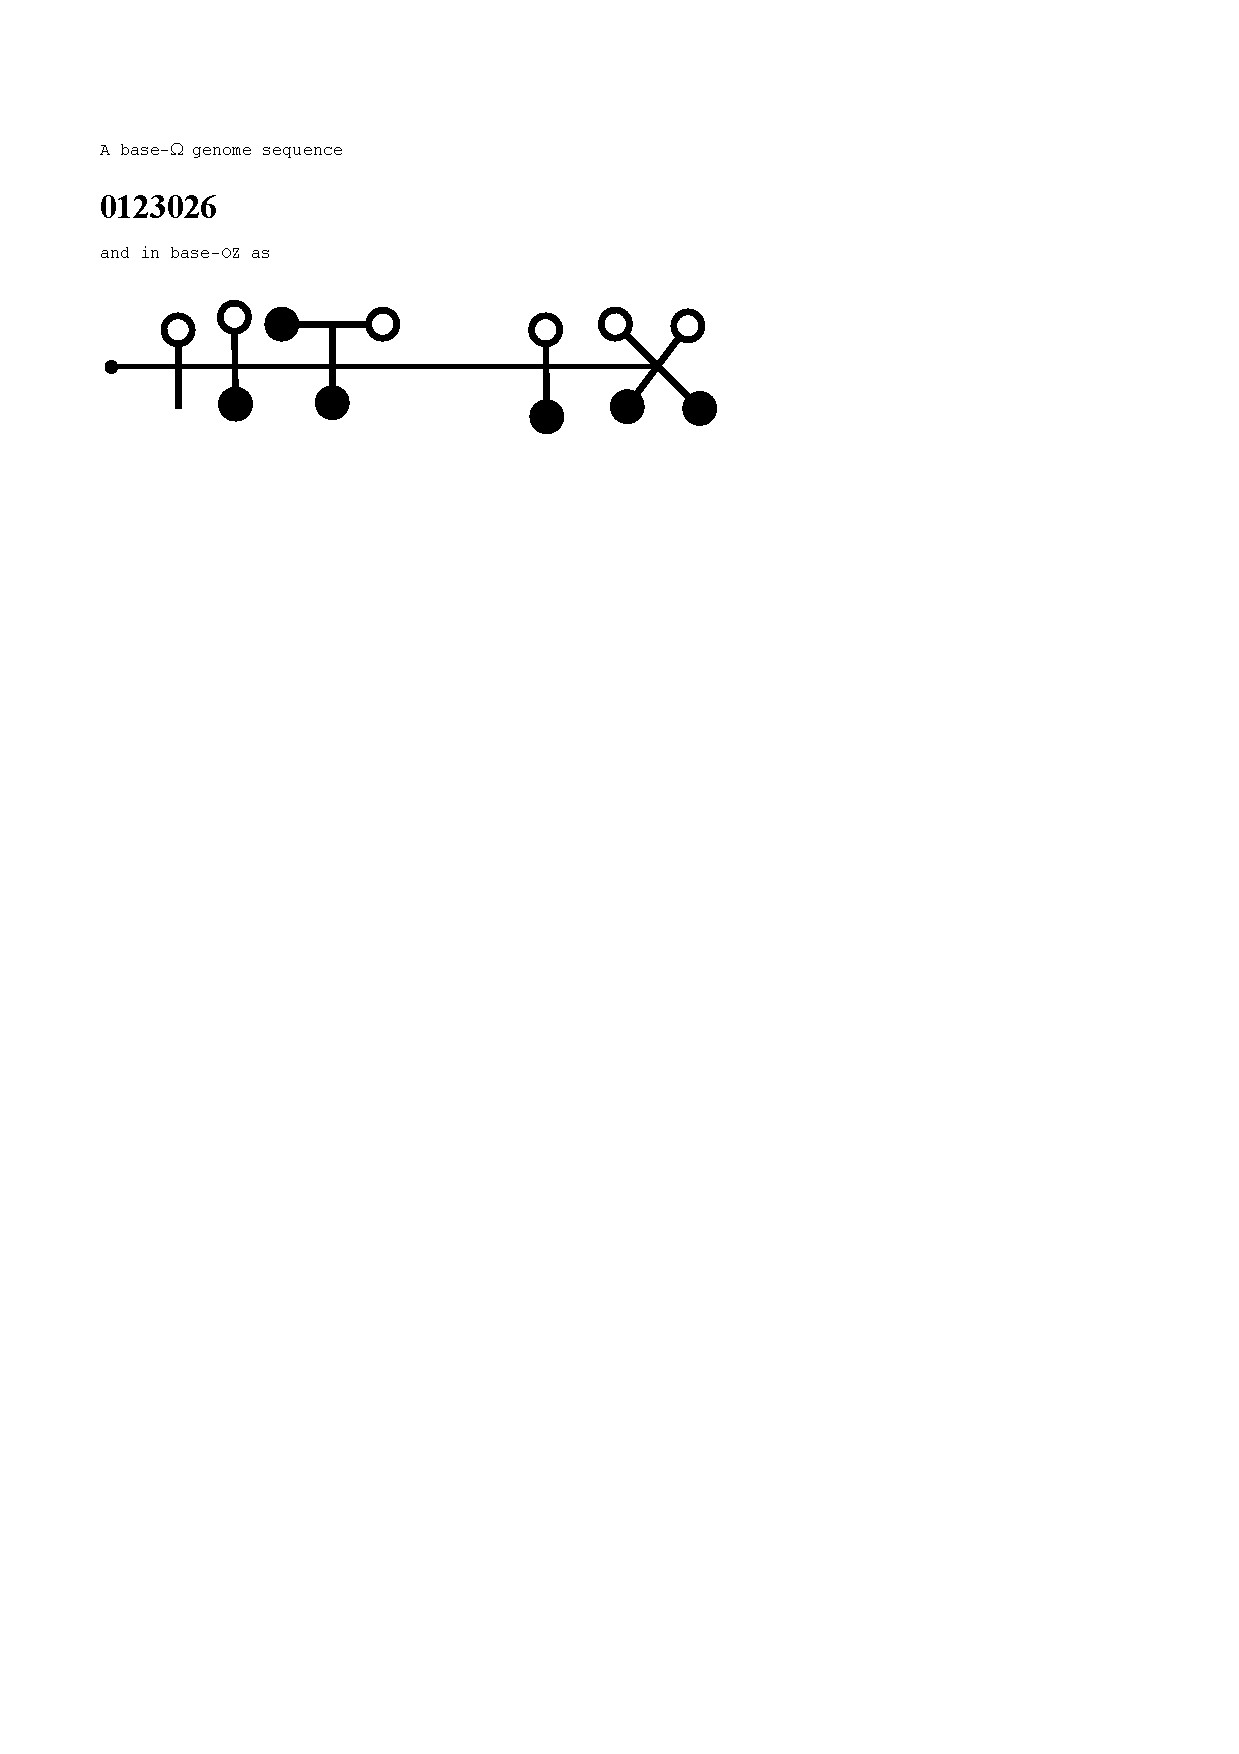
\includegraphics[trim=0cm 20cm 0cm 0cm, clip, width=0.9\textwidth,]{resources/pdfs/OZINCIPHER-APP3-EXA.pdf}\\
   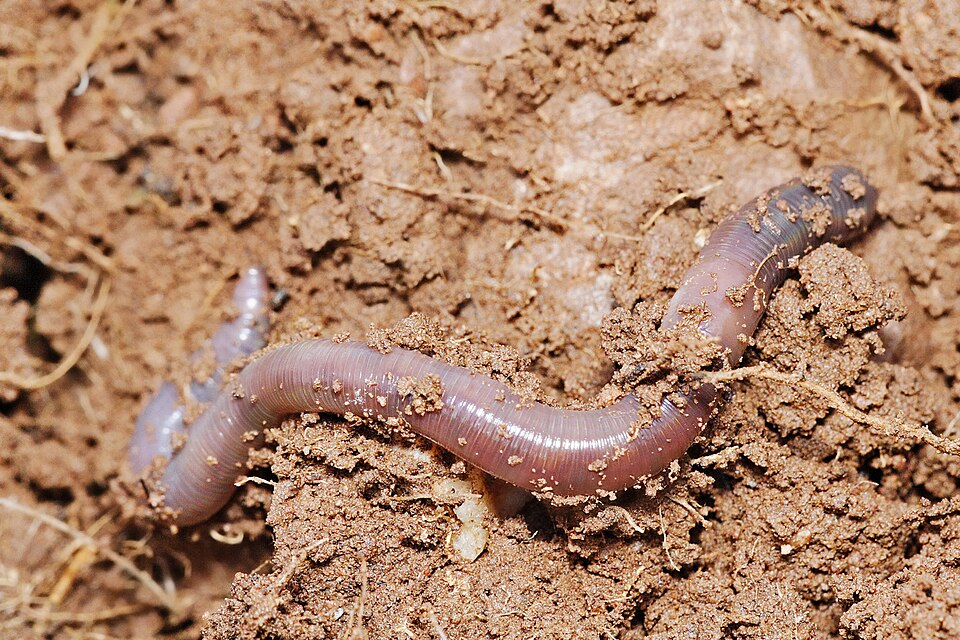
\includegraphics[trim=0cm 0cm 0cm 0cm, clip, width=0.9\textwidth,]{resources/images/Earthworm.jpg}\\
   \caption{An example of an actual organism from nature --- an Earthworm, for which, like the x-LGES rendering of the sequence $\Omega_{HiFinelle}$, results in a genome expression for a creature that almost looks the same at the HEAD and ROOT. Image sourced from Wikimedia Commons\cite{earthwormImage}.}
  \label{FIGEARTHWORM}
  \end{center}
\end{figure}





\subsection{x-LGES applied to named DNA Sequences}

Now that we have attained sufficient experience with expressing pure numeric sequences, we can return to actual na-Sequences, and checkout some potentially enlightening scenarios.

First, we shall want to have a way to assign meaningful names to our sequences. For example, the sequence from \textbf{\hyperref[TRANSSEQATG]{Transformation \ref{TRANSSEQATG}}}. Instead of just calling it $\Theta$, we could adapt a name from its corresponding na-Sequence, and then use that to distinguish it from other na-Sequences we shall want to compare it against.

Without caring whether it actually has a standard or conventional name based on its actual na-composition as depicted, we could adopt a system such as picking the first letters of its contained codons in the order they appear in the sequence, and then assign it a name based on the resulting acronym. So, we for example know from \textbf{\hyperref[TAB1]{Table \ref{TAB1}}} originally associated with that sequence, that the corresponding codons  by the code-names (also see \textbf{\hyperref[EQ4]{Equation \ref{EQ4}}}) are as follows:\\

\begin{equation}
\Theta = \langle Met, Lys, Leu, Amber \rangle
\end{equation}\\

So that we can just obtain a name for the sequence using the above suggested strategy as such:

\begin{trans}
$\langle Met, Lys, Leu, Amber \rangle \rightarrow \langle M, L, L, A \rangle \rightarrow MLLA$
\end{trans}

Thus, we might formally refer to our gene-program with a proper name as $\Theta_{MLLA}$ or just the \textbf{MLLA}-gene program --- where no confusion might arise, we shall just refer to it as $\Theta_{ml}$. 

So, how would this program's corresponding sequence appear if it were expressed in the \textbf{x-LGES}?

We have its corresponding $\Omega$-form expression in \textbf{\hyperref[TRANSSEQATG]{Transformation \ref{TRANSSEQATG}}}, so that\footnote{\textbf{NOTE} that, when encoding from na-Sequences constrained to just $\psi_{DNA}$ or $\psi_{RNA}$, then, the corresponding $\Omega-$base sequences shall always only span $\psi_{DD}$ (see \textbf{\hyperref[EQDNADIGSS]{Equation \ref{EQDNADIGSS}}}), but this need not be the case when mapping from $\psi_{na}$ to $\psi_{\Omega}$.}\\

\begin{equation}
\label{EQSEQMLLA}
\Theta_{ml} = \langle  1, 4, 3, 1, 1, 1, 4, 4, 1, 4, 1, 3 \rangle
\end{equation}\\

From that, we can leverage the pre-rendering calculus we have already encountered, well-applied in \textbf{\hyperref[TRANSGENSEQHiFinelle]{Transformation \ref{TRANSGENSEQHiFinelle}}}, and so that we can then readily apply \textbf{\hyperref[ALGCOZINPLATOEXT]{Algorithm \ref{ALGCOZINPLATOEXT}}} to $\Theta_{ml}$. The necessary derivation of the corresponding genome expression shall be as in: 

\begin{center}
\fbox{
\begin{minipage}{\textwidth}


\begin{trans}
\label{TRANSGENSEQMLLA}
$\Theta_{ml} = \langle 1, 4, 3, 1, 1, 1, 4, 4, 1, 4, 1, 3 \rangle \rightarrow \hbar(\overset{>}{\Theta_{ml}}) = \text{\textbf{1}6\textbf{4}4\textbf{3}2} \rightarrow \overset{>}{\Theta_{ml}} = \langle 1,4,3 \rangle \implies  m = \invpi(\overset{>}{\Theta_{ml}}) = 3 \implies  \boxed{\psi_{pf}}_{3} = \langle 7, 5, 3 \rangle$\\
$\implies \boxed{OZ(\Theta_{ml})} = \langle 7_{pf} \otimes 1_{oz},  5_{pf} \otimes 4_{oz}, 3_{pf} \otimes 3_{oz}\rangle$\\
$\implies \boxed{OZ(\Theta_{ml})}^* = \langle 1, 4, 3, 1, 1, 1, 4, 4, 1, 4, 1, 3 \rangle_{oz} \cdot \langle 7_{pf} \otimes 1_{oz},  5_{pf} \otimes 4_{oz}, 3_{pf} \otimes 3_{oz} \rangle \cdot \langle  1,4,3 \rangle_{oz}$
\end{trans}


\end{minipage}}
\\
\end{center}

And the corresponding, fully rendered \textbf{FGE} would be as depicted in \textbf{\hyperref[FIGLGESMLLA]{Figure \ref{FIGLGESMLLA}}} hereafter.

\begin{figure}[H]
  \begin{center}
  %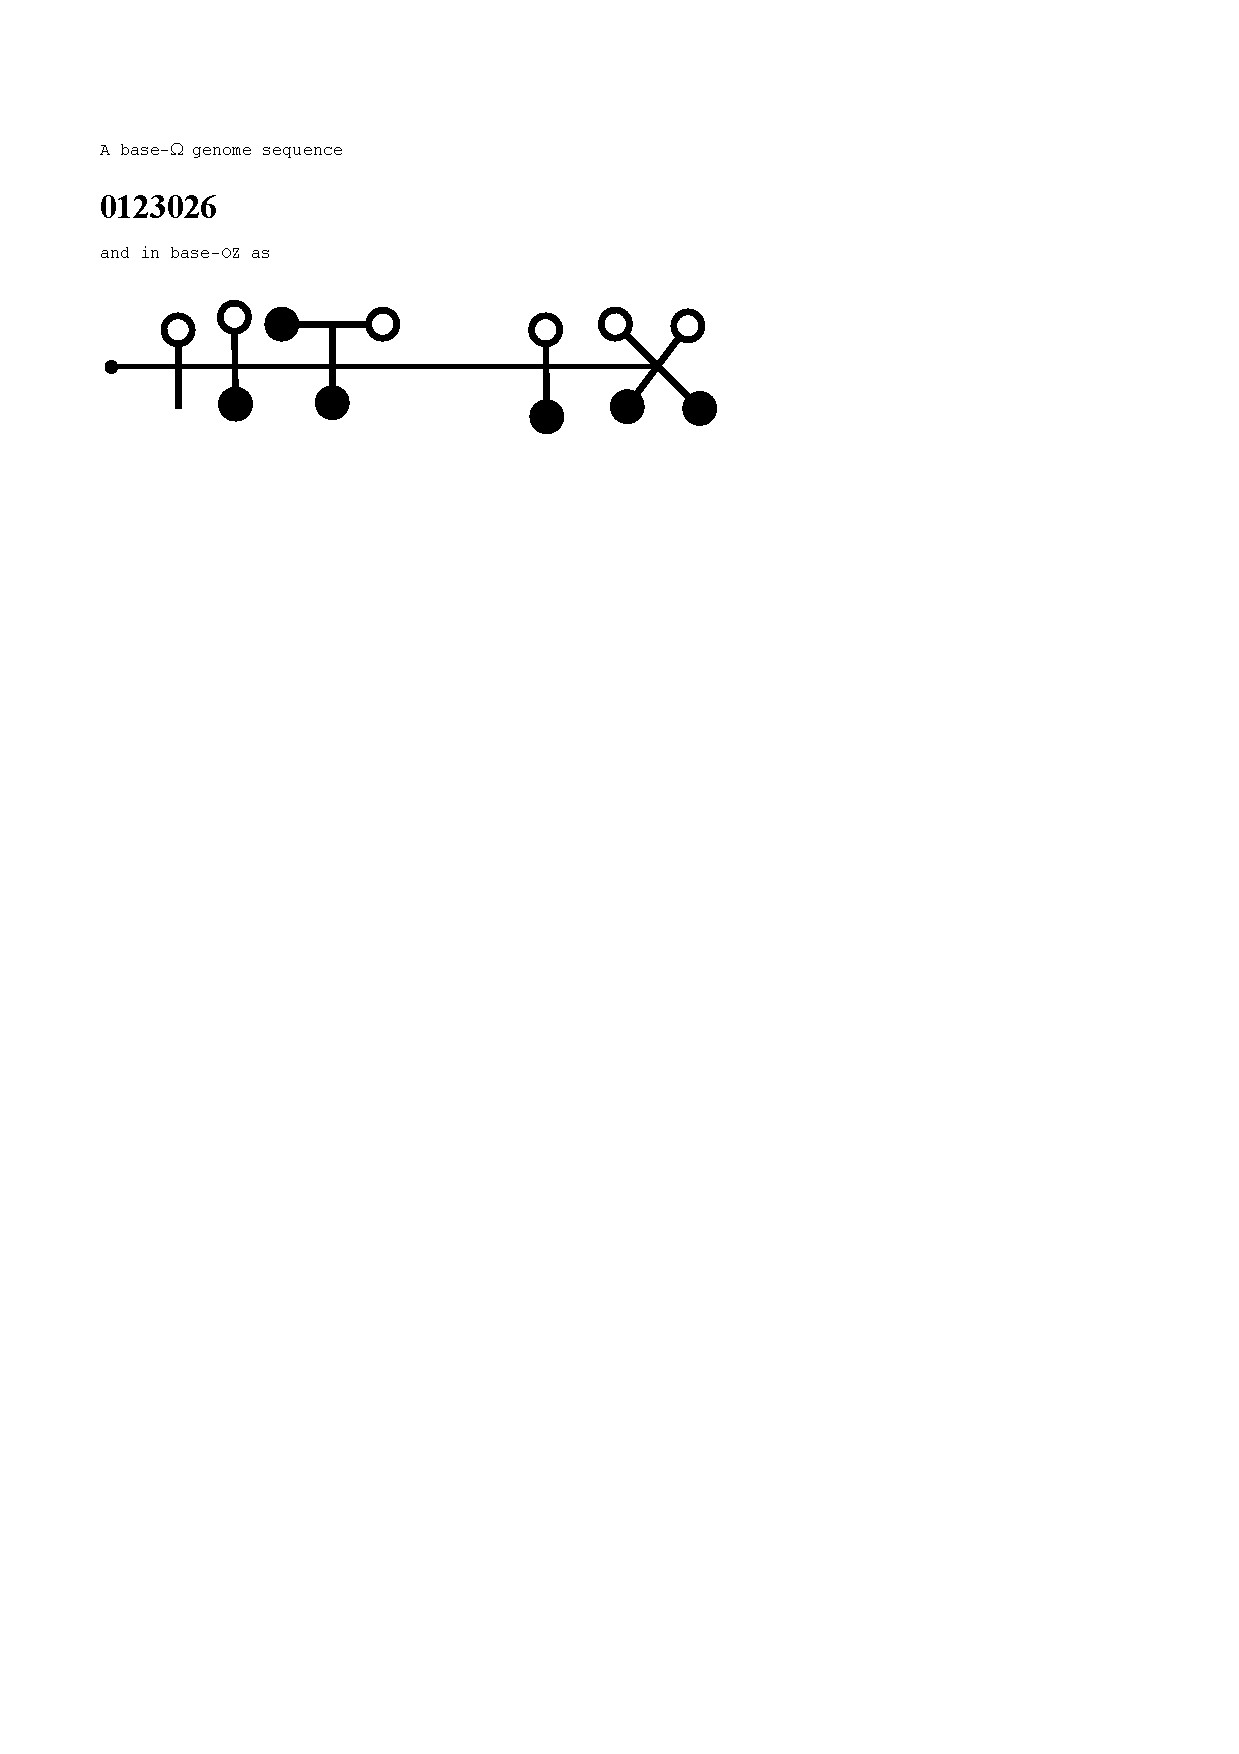
\includegraphics[trim=0cm 20cm 0cm 0cm, clip, width=0.9\textwidth,]{resources/pdfs/OZINCIPHER-APP3-EXA.pdf}\\
   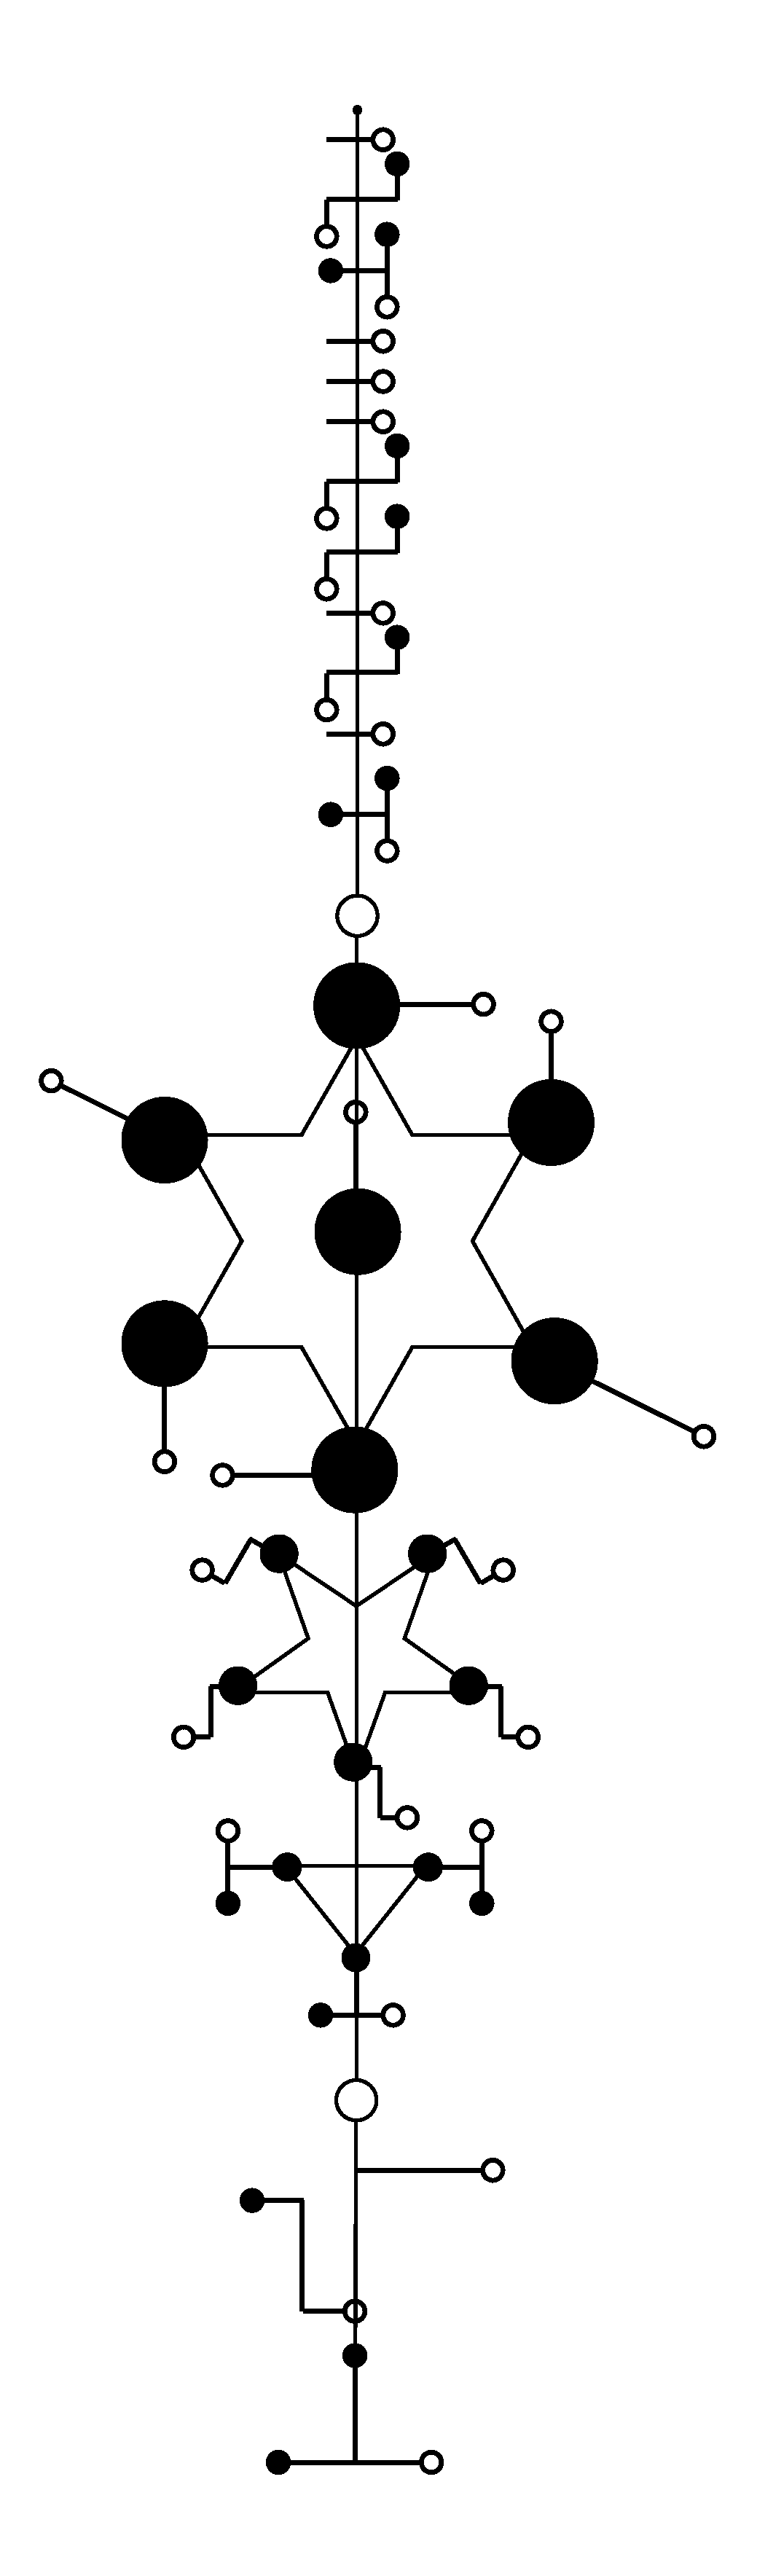
\includegraphics[trim=0cm 0cm 0cm 0cm, clip, height=0.9\textheight,]{resources/pdfs/xLGES-PLATONIC-MLLA-landscape.pdf}\\
   \caption{The \textbf{x-LGES form rendering} of the sequence $\Theta_{mlla}$, depicting its complete \textbf{FGE} with HEAD, BODY and ROOT segments.}
  \label{FIGLGESMLLA}
  \end{center}
\end{figure}


Thus we conclude our treatment of TRANSFORMATICS in GENETICS.



\chapter{Conclusion}
\label{CONC}

%---refs fixed up to this point...


In this book\footnote{Originally, first a paper, then a monograph, and finally a mini-treatise!}, we have advanced our knowledge concerning the important and fundamental subject of genetics with new theory and practical ideas previously only held informally or totally unknown. We have explored several useful and interesting ways by which the newly proposed mathematical field of inquiry, known as \textbf{TRANSFORMATICS} --- potentially a sub-field of/fusion of mathematical statistics and linear algebra\footnote{As in the conclusion of the original transformatics paper\cite{transformatics}, the author strongly feels that in the future, and with further investments in research, development of theory and applications, transformatics might become its own sub-field of mathematics, distinct from both statistics and linear algebra, but also, though inspired by sequence processors in computer science, also more general than or distinct from that field too.}, might be applied in the sub-field of the biological sciences known as \textbf{GENETICS}. 

Though much of the work was mathematical in nature, we have also had lots of useful theory presented and some only proposed, in the form of conceptual and especially philosophical ideas relating to how to understand or explore genetics through the lens of a sequence analyst or processor. 

In terms of concrete \textbf{Key Metrics and Contributions} this single work has brought to surface:
\begin{enumerate}
\item{ \textbf{16 Working Definitions} were developed in relation to various concepts in analytical genetics, sequence analysis and sequence processing in general (including 3 \textit{Extra Definitions} not directly under Genetics, but also meant to demonstrate how Transformatics could be leveraged/applied --- in Physics: refer to Appendix  \textbf{\hyperref[SECFUTDIRECT]{Chapter \ref{SECFUTDIRECT}}}), and these include:

	\begin{enumerate}
	\item The \textbf{na-Sequences} --- see  \textbf{\hyperref[DEFNASEQ]{Definition \ref{DEFNASEQ}}}
	\item The \textbf{START-Codons} --- see \textbf{\hyperref[DEFSTARTCOD]{Definition \ref{DEFSTARTCOD}}}
		\item The \textbf{STOP-Codons} --- see \textbf{\hyperref[DEFSTOPCOD]{Definition \ref{DEFSTOPCOD}}}
	\item The \textbf{Sequence Characteristic} --- see  \textbf{\hyperref[DEFSEQCHAR]{Definition \ref{DEFSEQCHAR}}}
	\item The \textbf{Population Characteristic} --- see  \textbf{\hyperref[DEFPOPCHAR]{Definition \ref{DEFPOPCHAR}}}
	\item The \textbf{Genome Sequencer} --- see  \textbf{\hyperref[DEFGENOMESEQ]{Definition \ref{DEFGENOMESEQ}}}
	\item The \textbf{Ribosome} --- see  \textbf{\hyperref[DEFRIBOSOME]{Definition \ref{DEFRIBOSOME}}}
	\end{enumerate}

}
\item{ \textbf{4 Theorems} were developed and presented for the first time, spanning genetic sequences and then sequence complements in general. These include...

	\begin{enumerate}
	\item \textbf{Complement Sequences} --- see  \textbf{\hyperref[THEOCOMPLEMENTS]{Theorem \ref{THEOCOMPLEMENTS}}}
	\item \textbf{Complement of an o-SSI is an o-SSI} --- see  \textbf{\hyperref[THEOCOMPLOSSI]{Theorem \ref{THEOCOMPLOSSI}}} 
	\item \textbf{Equivalence of Sequences} under the Complement Transform  --- see  \textbf{\hyperref[THEOCOMPEQUIV]{Theorem \ref{THEOCOMPEQUIV}}} 
	\end{enumerate}
}
\item {\textbf{3 Laws} were distilled and presented for the first time:
	\begin{enumerate}
	\item \textbf{\hyperref[LAWNA]{Law \ref{LAWNA}}}: Concerning the nucleic acid identifier symbol set, $\psi_{na}$. 
	\item \textbf{\hyperref[LAW2]{Law \ref{LAW2}}}: Concerning Introns: Non-coding gene-programs.
	\item \textbf{\hyperref[LAWGDL]{Law \ref{LAWGDL}}}: The \textbf{Identity Genome Sequence} Law.
	\end{enumerate}
}
\item{ \textbf{16 Transformers} were developed and presented for the first time, including...

	\begin{enumerate}
	\item The formal definition of the \textbf{Ribosome} as a \textbf{Protein Generator} (\textbf{\hyperref[TRANSF3]{Transformer \ref{TRANSF3}}})
	\item The \textbf{n-Gram Generator} (\textbf{\hyperref[TRANSFBUND]{Transformer \ref{TRANSFBUND}}})
	\item The \textbf{Sequence Look-up System} that leverages G$\ddot{o}$del numbers for efficient DNA-database queries (\textbf{\hyperref[TRANSFSEQLOOKUP]{Transformer \ref{TRANSFSEQLOOKUP}}})
	\item The \textbf{Random Sequence/Symbol Generator} that can construct random DNA/RNA sequences, but also any arbitrary random\footnote{We could have wanted to generalize this generator so that it can also handle the case of non-random sequence generation --- especially since it already bases its generated sequence on the properties of some input sequence, so that for example we can generate sequences that reflect the symbol distribution within the input/sample sequence (something akin to how a ChatGPT model can generate new text based on/related to some samples with say non-uniform symbol distributions), but we chose to not do that within the context of this present work, and shall leave that for a future publication and treatment.} sequence (\textbf{\hyperref[TRANSFRSG]{Transformer \ref{TRANSFRSG}}})
	\item A transformer for converting between pure numbers (in base-10) into DNA/RNA code, and vice-versa --- the $\psi_{na}$ to $\psi_{10}$ \textbf{na-to-Decimal Decoder} (\textbf{\hyperref[TRANSFDECTONASEQ]{Transformer \ref{TRANSFDECTONASEQ}}})
	\end{enumerate}
	
	and many more simple and some complex, but essential transformer utilities and specifications.

}
\item{ \textbf{30 Transformations} were presented to help advance generic as well as particular computational solutions to many kinds of basic problems in sequence analysis, processing and several concerning gene/genome expression problems, including some special ones such as:

	\begin{itemize}
	\item \textbf{\hyperref[TRANSGENSEQ]{Transformation \ref{TRANSGENSEQ}}} that generalizes the intricate process of generating a correct \textbf{consensus genome sequence} via \textbf{genome sequencing}.
	\item \textbf{\hyperref[TRANSGENSEQHiFinelle]{Transformation \ref{TRANSGENSEQHiFinelle}}} that serves as a good template for the intricate process underlying the \textbf{derivation of a Full Genome Expression} from a plain sequence using the \textbf{x-LGES}.
	\end{itemize}

 }
\item{\textbf{8 Algorithms} were developed and presented for the first time, including:
	\begin{enumerate}
	\item \textbf{\hyperref[ALGCSA]{Algorithm \ref{ALGCSA}}}: The \textbf{Closest Sequence Algorithm}.
	\item \textbf{\hyperref[ALGtMCS]{Algorithm \ref{ALGtMCS}}}: The \textbf{tMCS} Algorithm for computing the Maximum Common Subsequence.
		\item \textbf{\hyperref[ALGLUSHUFFLEA]{Algorithm \ref{ALGLUSHUFFLEA}}}: The \textbf{First Lu-Shuffle Algorithm} (FLSA): $\text{lu\_shuffler\_a}(\Theta, k)$.
	\item \textbf{\hyperref[ALGLUSHUFFLEB]{Algorithm \ref{ALGLUSHUFFLEB}}}: The \textbf{Second Lu-Shuffle Algorithm} (SLSA): $\text{lu\_shuffler\_b}(\Theta, k)$.
	\item \textbf{\hyperref[ALGCOZIN]{Algorithm \ref{ALGCOZIN}}}: The \textbf{$\Omega$-to-OZIN Genetic Code Transcription Algorithm}.
	\item \textbf{\hyperref[ALGCOZINPLATO]{Algorithm \ref{ALGCOZINPLATO}}}: The \textbf{$\Omega$-to-PLATONIC Form Genetic Code Expression Algorithm} --- chosen as core of \textbf{LGES}, leverages \textbf{PFEK} translation keys to process BODY/THORAX aspect of \textbf{FGE}.
	\item \textbf{\hyperref[ALGCOZINPLATOEXT]{Algorithm \ref{ALGCOZINPLATOEXT}}}: The \textbf{x-LGES Algorithm} --- extends \textbf{LGES} with processing of a ROOT/SUFFIX component.

	\item \textbf{\hyperref[ALGCOZINPLATO_ORIG]{Algorithm \ref{ALGCOZINPLATO_ORIG}}}: The [original] \textbf{LGES Algorithm} --- renders the genome expression using complement sequences.
	\end{enumerate}
}
\item \textbf{3 Tabular Analyses} were presented, including \textbf{\hyperref[TABFAN]{Table \ref{TABFAN}}} that depicts how to perform comparative statistical analysis of DNA, RNA or any na-Sequence using some measures and methods from transformatics.
\item \textbf{Overall, a total of 7 Tables} were presented, including the two critically important \textbf{PFEK} tables \textbf{\hyperref[TABSSLAPERK]{Table \ref{TABSSLAPERK}}} and \textbf{\hyperref[TABFSLAPERK]{Table \ref{TABFSLAPERK}}} for helping in computing predictable shuffles/anagrams of the base-10 n-SSI using the \textbf{SLSA} and \textbf{FLSA} algorithms respectively.
\item{ \textbf{2 Original Ciphers} --- very rare and universally usable cryptographic keys were presented as part of the \textbf{Lu-Genome Expression System}, as well as proper justification for their practical relevance and sufficient historical background and example applications of both.

\begin{enumerate}
\item The \textbf{OZIN Cipher} key depicted in \textbf{\hyperref[FIGOZIN]{Figure \ref{FIGOZIN}}}
\item The \textbf{PLATO Cipher} key depicted in \textbf{\hyperref[FIGPLATONICCIPH]{Figure \ref{FIGPLATONICCIPH}}}
\end{enumerate}

}
\item \textbf{3 Core Problems} in the matter/domain of \textbf{Genome Sequencing} were formally defined and their theoretical solutions also presented\footnote{\textbf{FUTURE WORK:} We could have delved into actually demonstrating how to use the proposed theory and solutions to conduct actual genome sequencing, especially by hand, however, I have decided to postpone that to a later publication or edition of this book.}. Refer to  \textbf{\hyperref[SEC3COREPROB]{Section \ref{SEC3COREPROB}}} or \textbf{\hyperref[SECMATHSEQ]{Chapter \ref{SECMATHSEQ}}}.

\item{ \textbf{More than 10 Source Code Examples}, some in the TEA language (by the author\cite{cli_tttt}), and relating to conducting quick analyses of arbitrary na-Sequences via the commandline (refer to \textbf{\hyperref[SECFANAL]{Section \ref{SECFANAL}}}), and 8 (in \textbf{\hyperref[SECRSG]{Chapter \ref{SECRSG}}}), related to how to generate arbitrary random sequences using Python and the proposed \textbf{RSG} Transformer Machine:

\begin{enumerate}
\item \textbf{\hyperref[LST_FLSA]{Listing \ref{LST_FLSA}}} --- The First Lu-Shuffle Algorithm.
\item \textbf{\hyperref[LST_SLSA]{Listing \ref{LST_SLSA}}} --- The Second  Lu-Shuffle Algorithm.
\item \textbf{\hyperref[LST_USYMBOLSET]{Listing \ref{LST_USYMBOLSET}}} --- Generate Unspecific Symbol Set for Any Sequence.
\item \textbf{\hyperref[LST_PROTRACT]{Listing \ref{LST_PROTRACT}}} --- Multiply any Sequence by a given factor.
\item \textbf{\hyperref[LST_RNG]{Listing \ref{LST_RNG}}} --- Generate a Random Number within a specified range.
\item \textbf{\hyperref[LST_SHUFFLE]{Listing \ref{LST_SHUFFLE}}} --- Shuffle/Anagrammatize a sequence using no other parameters.
\item \textbf{\hyperref[LST_SELECT]{Listing \ref{LST_SELECT}}} --- Select a specific number of items from some sequence.
\item \textbf{\hyperref[LST_RSG]{Listing \ref{LST_RSG}}} --- Generate a random sequence of a specified length and whose terms derive from the symbol set of a specified input sequence.
\end{enumerate}

}
\item And many other quantifiable and unquantifiable major and minor contributions to genetics, mathematics, computer science, philosophy and more.
\end{enumerate}

\vspace{1em}

Thus, we set out to explore ways to leverage as well as further the newly proposed discipline of \textbf{Transformatics}, by using it to explain problems in \textbf{Genetics}\footnote{Which happens to be one of the major, fundamental sciences that hinges much on the concept of sequences, their processing and analysis.}, but also, so as to be able to use it to derive or develop solutions to any such problems we identify and find tractable under the theory and mechanics of sequence transformers. 

In this regard, as highlighted in the enumerations above, we have formalized many working definitions of important fundamental concepts (from a transformatic-analytical point-of-view) spanning symbol sets, various statistical measures applicable to sequences, several abstract machines applicable to specific and general problems in genetics and more. 

We have distilled some useful general results in the form of theorems, have immortalized some critical and relevant laws relating to genetic code sequences, have extensively demonstrated how the concept of modeling general solutions to various problems can be accomplished using the notion of [re-usable] transformers --- defined not in programming code as some might think, but as mathematical operators usable with or without computers. We have demonstrated how such transformers can be leveraged to solve specific or particular practical problems via numerous well-structured transformations. 

We have invented and presented some new algorithms that would allow the concepts and solutions we developed in transformatics theory for various problems to be readily turned into computable solutions using any programming language. And in this regard, have also gone ahead to demonstrate the implementation of some practical solutions or fundamental aspects of them using source-code implementations in both TEA and Python that anyone can merely copy from the text and apply to their specific problems or which one could adapt so as to build more elaborate computational solutions to problems not just in genetics, but also for general sequence analysis and processing problems. 

We have demonstrated ways to leverage statistical analysis so as to make sense of differences in and quantifiable similarities between two or more sequences --- DNA related or not. We have also presented some reference tables that would help anyone attempting to leverage the proposed theory and algorithms of the \textbf{Lu-Genome Expression System} to be able to readily do so without having to guess or dive into the daunting process of generating \textbf{Platonic Form Encoding Keys} by hand. 

Related to the \textbf{LGES}, we have also presented and demonstrated for the first time, two very interesting and universally usable [originally esoteric] ciphers that would help not in genetics-related cryptography problems, but in helping both students and researchers of genetics to readily explore and communicate otherwise difficult to express concepts relating to genetic diversity, genetic similarity, the consequences of genetic mutations --- additions, subtractions or alterations to genetic sequences, etc. using a visual language that is reminiscent of actual molecular-level expressions resulting from the natural processing of DNA and mRNA code, all the way up to the expression of entire organisms from mere genetic code. 

With regards to understanding or explaining how a full genome might be derived from bits of DNA sequence read from or known, concerning an individual organism, an individual species, a genus, an entire family or populations of organisms, we have advanced the literature by developing rigorous mathematical concepts and solutions to the matter of genome sequencing whether performed by hand as in the classical context of Fred Sanger, or with advanced computation such as in modern genome banks and DNA processors. 

Overall, this book, though it originally started out as just a paper, and though some would envision it to have been a longer treatise than it actually is, surely has helped lay the ground for much future work in genetics, the mathematical sciences as well as in transformatics itself, so they can take advantage of and leverage the methods, theory and mechanics/calculus of transformatics as presented in this work, and especially so that it makes easier, the definition of new problems, design new solutions to existing as well as new problems, but also, so that it is possible to readily take many ideas previously either intractable or only appreciable in theory, into the practical domain --- especially via computational methods leveraging sequence transformers.

It is in the dreams and hopes of the author, that the work that started with the treatment of basic sequences in the form of pure number expressions --- see \textbf{GTNC}\footnote{The original paper actually first got written circa 2020: \url{https://scholar.archive.org/work/apn4f26kdzatfodrap7avqafce}}\cite{Lutalo2024gtnc}, circa 2020, while only getting started with their MSc and at that time\footnote{Joseph, despite having been very active in the contemporary scientific and mathematical research community (see ORCID: \url{https://orcid.org/0000-0002-0002-4657}), still hasn't been generally well appreciated --- they are still not affiliated with any academic institution or faculty, have not managed to secure a teaching position despite much of their work contributing to global open-learning via the Internet (see \url{https://t.me/bclectures} and \url{https://www.youtube.com/playlist?list=PL9nqA7nxEPgv_CqHOxIDj2Jf1gHAEV-B-}), and despite having expressed interest in pursuing their PhD in either Computer Science or Mathematics at Oxford\cite{lutalo_2025_sop}, haven't yet secured a PhD position nor scholarship.}, only looking at sequences as though they were a concept native to only \textbf{number theory}, does not stop with recent advances such as the \textbf{LNS}\cite{lnspaper} that started to explore these ideas in the context of physics and computer science, and then \textbf{ADT} that ushered in the sensibilities of mathematical statistics, but that transformatics and the collective mathematical theories of treating of sequences of symbols via transformers and analytical specifications, gets its own wings and finally flies off the ground into any and all fields of inquiry with useful results and advancements of human understanding and knowledge. 


\section{Future Directions}
\label{SECFUTUREDIRECT}

In this single work, several issues, problems and potential areas of further research and inquiry have been identified, as well as highlighted all throughout the book. For purposes of bringing attention to the key points thus identified, we shall only enumerate them as highlights and in brief:

\begin{enumerate}
\item \textbf{Pathological Gene Programs:} Given we isolated the START and STOP codons that regulate or constrain how protein synthesis is conducted at the ribosome level, we wish to establish if there might exist malicious gene programs that might exploit the ribosome's na-Sequence processing logic so as to cause problems such as failure to manufacture some necessary proteins or amino-acids (due to absence of or misplacement of START-codons), but also the terrible, pathological case where a ribosome starts to construct a protein (as an amino-acid chain), but fails to return/complete since it is presented with an infinitely long or non-terminating gene program. \textbf{Refer to \textbf{\hyperref[SECSYMBOLSETSNGRAMS]{Section \ref{SECSYMBOLSETSNGRAMS}}}}

\item \textbf{Automatic Sequence Characteristic:} Having established the fundamental relevance of the modal sequence statistic, as well as the more elaborate sequence characteristic measure and its usefulness in several aspects of genetic sequence analysis and processing (similarity tests, classification problems, genome expression, etc.), we wish to make sure that there is a simple and straightforward way by which, when presented with a sequence of symbols such as the complete genome sequence of some organism stored in a flat text file, we can automatically compute and present the corresponding sequence characteristic statistic. This, especially via use of the TEA programming language on the command line. \textbf{Refer to \textbf{\hyperref[SECFANAL]{Section \ref{SECFANAL}}}}

\item \textbf{Evaluate G$\ddot{o}$del Number Indices for na-Sequences:} Since we realized that computation of and use of special indices --- in the form of hash keys, corresponding to especially very long na-Sequences (such as those of the human genome that might shoot into millions and up to billions of symbols) might help lessen the space-time complexity with regards to storage, lookup and comparison of na-Sequences as in a database system, we shall want to empirically and theoretically establish if use of G$\ddot{o}$del numbers (especially when combined with use of a sequence's modal statistic or sequence characteristic) might offer an optimal solution for storage, lookup and comparison of large or arbitrarily long na-Sequences. \textbf{Refer to \textbf{\hyperref[SECSEQSTORAGE]{Section \ref{SECSEQSTORAGE}}}}

\item \textbf{Implementing Entropy Sources:} Especially because, as we have identified in several problems and solutions concerning sequence processing (shuffling, anagrammatizing, sequence generation, etc.), but also in genetics (simulation of meiosis, genome expression, etc) that use of and generation of/harnessing of randomness is fundamentally important, we shall want to ascertain, and especially both in theory and with empirical computable solutions, how we can produce randomness from scratch, and especially in a closed-system or with mere pen and paper. And to ascertain whether such is actually feasible or not. \textbf{Refer to \textbf{\hyperref[SECRNGFUNC]{Section \ref{SECRNGFUNC}}}} 

\item \textbf{Further Computational Model of The Ribosome:} Since we have already embarked on developing, presenting and exploiting a computational model for the protein synthesis mechanism in living cells, and have managed to not only develop a formal process that captures the gist of how a ribosome works, it raises new and important extra problems for the computer scientist studying the ribosome, and which problems we would want to find reliable answers for. These include the matter of the Instruction Set of the Ribosome Machine, its computer architecture and how it relates to the von Neumann Architecture, whether or not the ribosome is Turing Complete, how we might implement a virtual or robotic ribosome etc. \textbf{Refer to \textbf{\hyperref[SECPROT]{Section \ref{SECPROT}}}} 

\item \textbf{Concerning the Relationship Between DNA, Psychology and Spirituality:} Though it might not directly fall in the domain of pure genetics, it shall be interesting and very likely rewarding if not enlightening, to study, explore and expound on the matter or problem of whether it is indeed true (or false) that genetics underlies the spiritual-functions in a human? Could genetics explain or underlie peculiarities in human psychology both at an individual as well as from the context of entire communities, families, nations or an entire species? Since artificial (though intelligent) constructs such as robots and AGIs don't share the same material basis as does living things --- in the sense that they aren't controlled/limited by nor based on organic tissue, no semblance of genetic code underlying their expression or functions\footnote{Of course, one might argue, and plausibly so, that artificial intelligences are nonetheless designed by and brought to life by humans who are controlled or limited by genetics, and also, there is a strong community in computing, that bases the design and implementation of artificial systems on not just code that somewhat is reminiscent of genetic code, but also which directly or indirectly mimics natural/biological systems such as neural networks in living things, but also use of genetic programming for optimizing self-regulating learning algorithms, etc. But, this point here, specifically refers to whether or not such artificial constructs are directly built with or using natural, genetic material... bio-automata constructed out of actual living tissue or synthetic organisms that can exist around or inside living things might otherwise cause us to relax this stressed point.}, etc. Could it be that they can't exhibit or participate in the same spiritual, psycho-spiritual, or even preternatural phenomena that living things (especially humans), seem to be inseparable from?  \textbf{Refer to \textbf{\hyperref[SECPROT]{Section \ref{SECPROT}}} and \textbf{\hyperref[SECFUTDIRECT]{Chapter \ref{SECFUTDIRECT}}}} 

\item \textbf{Establish Bounds on Protein or Amino-Acid Chain Relative to Gene Program:} While formalizing the concept of gene expression in living things, and especially when dealing with the matter of how na-Sequences get translated into an amino-acid chain, and thus into a protein, a problem arose; since it is that most of the protein manufacturing process is somewhat linear and especially a matter of 1-to-1 encoding or translation of genetic code into other materials, it would be useful to prove or perhaps clarify on whether it is true that the length of a gene-program (since it is essentially the chain of codons that eventually get translated into the protein) imposes a finite limit on the length of the material (such as a protein or amino-acid chain) that a ribosome can produce from a particular genetic code sequence? \textbf{Refer to \textbf{\hyperref[SEC5]{Section \ref{SEC5}}} and especially \textbf{\hyperref[TRANSF2]{Transformer \ref{TRANSF2}}}} 


\item \textbf{Genetics and Mysticism, Genetic Veves:} So, despite this being a book on especially the mathematics of genetics and sequence analysis, we did come across important matters (especially for the \textit{humanities} and philosophy) concerning the (not-very surprising) role genetics and especially genetic code might play in humane culture, the arts and traditions across the world. Particularly, while studying and developing the \textbf{LGES}, we found that the systematic diagrams --- the \textbf{FGEs}, derivable from or expressing particular na-Sequences as well as any numeric sequence, have so many similarities to or that they are somewhat reminiscent of concepts such as sacred geometry, voodoo veves, magical seals and sigils, psycho-cultural archetypes, etc. from various contexts, cultures and traditions all over the world. Is it just because of the fact that geometry and geometrical forms are generally universal and cut-across cultures, space and time, or is there something deeper, perhaps not immediately discernible concerning our \textbf{Lu-Genome Expression System} that might hint at critical aspects of universal human culture, mysticism as well as spirituality? Could a genetic veve disrupt contemporary voodoo veves or traditional cabalistic seals when considered from the perspective of visual-spatial glyphs that speak to the human subconscious for example? \textbf{Refer to \textbf{\hyperref[SECFULLGES]{Section \ref{SECFULLGES}}}} 


\item \textbf{Practical Genome Sequencing:} We have laid down most, if not all of the necessary theoretical and conceptual machinery for how to go about practically solving the matter of reducing a collection of sequences to their most correct, representative genome sequence. However, in this work, we have not actually gone ahead to demonstrate how this theory shall be applied or utilized, say with sample na-Sequences much as we have done this for most of the other problems and concepts we have tackled in the book. Thus, future work shall need to expound on this with illustrative or representative examples and complete solutions to how to perform actual genome sequencing for genetic code first of all, but also, and given the theory can be applied to any kinds of symbol sequences, for arbitrary scenarios too.  \textbf{Refer to \textbf{\hyperref[SECMATHSEQ]{Chapter \ref{SECMATHSEQ}}}} 


\end{enumerate}



%---[ END BOOK CONTENT/CHAPTERS ]

%---[ BEGIN BOOK END/APPENDICES]
\begin{appendices}

\chapter{Other Functions of DNA Beyond Protein Synthesis}
\label{APPOTHERFUNC}


While most of this book focused on DNA's most well-known function as the material basis for how the protein synthesis process is made possible, but also how it is regulated in nature, and yet, protein synthesis is not all that DNA is useful for! As any newcomer to genetics and nucleic-acid sequences might wonder --- \textbf{What else is DNA used for apart from the construction of proteins?} And so, I posed this question to my research assistant\cite{copilot_dna_assistant}, and the answer here shared, almost verbatim, might help lift others out of darkness too...


\vspace{2em}

\textbf{Deoxyribonucleic acid} is widely known for its role in protein synthesis, however, it also serves several other critical functions in biological systems as enumerated in summary here:

\begin{enumerate}
    \item{ \textbf{Regulation of Gene Expression\cite{alberts2002molecular}} 
    

	\begin{itemize}
	\item Non-coding DNA (which makes up $\approx 98–99$\% of the genome) contains regulatory elements like enhancers, silencers, and promoters.
	\item These regions control \textit{when}, \textit{where}, and \textit{how much} a gene is expressed --- like how a conductor would guide and regulate a symphony's performances.
	\end{itemize}	    
    
    }

    \item{ \textbf{Epigenetic Control\cite{bird2007perceptions}} 

\begin{itemize}
	\item DNA interacts with histones and chemical tags (like methyl groups) to form chromatin, which can be tightly or loosely packed.
	\item This packing determines gene accessibility, influencing cell identity and response to environmental factors like stress or diet.
	\end{itemize}	    
    
    
    }

    \item{ \textbf{DNA Repair and Replication\cite{friedberg2006dna}} 
    
    \begin{itemize}
	\item DNA contains built-in mechanisms for self-repair and accurate replication, ensuring genetic fidelity across cell divisions.
	\item Specialized sequences help detect and correct errors, preventing mutations that could lead to disease.
	\end{itemize}	 

    
    
    }

    \item{ \textbf{Cell Differentiation and Development\cite{gilbert2010developmental}} 
    
        \begin{itemize}
	\item Though every cell has the same DNA, different genes are turned on/off to create neurons, muscle cells, skin cells, etc.
	\item This selective expression is orchestrated by DNA’s regulatory architecture and chromatin dynamics.
	\end{itemize}
    
    
    So, although all cells share the same DNA, selective gene expression enables differentiation into various cell types such as neurons, muscle cells, and epithelial cells .
    
    
    }

    \item{ \textbf{Evolutionary Adaptation\cite{king1975noncoding}} 
    
            \begin{itemize}
	\item Non-coding regions accumulate mutations without affecting protein function, serving as a sandbox for evolutionary innovation.
	\item These changes can influence species traits, adaptation, and even speciation over time.
	\end{itemize}
    
    
    }

    \item{ \textbf{Biological Memory and Identity\cite{jacob1977evolution}} 
    
     \begin{itemize}
	\item DNA acts as a biological archive, encoding ancestral information and evolutionary history.
	\item When considering context-aware symbolic systems and the matter of \textit{cultural abstraction}, then DNA can also be seen as a \textbf{modal sequence} that bridges biology and [symbolic] meaning.
	\end{itemize}
  
    }
\end{enumerate}


\chapter{Origins of the OZIN Cipher}
\label{APPOZIN}

\begin{figure}[H]
  \begin{center}
  %\includegraphics[trim=2cm 8cm 2cm 8cm, clip, width=0.9\textwidth,]{resources/pdfs/ProteinSynthesisStateMachine.pdf}\\
   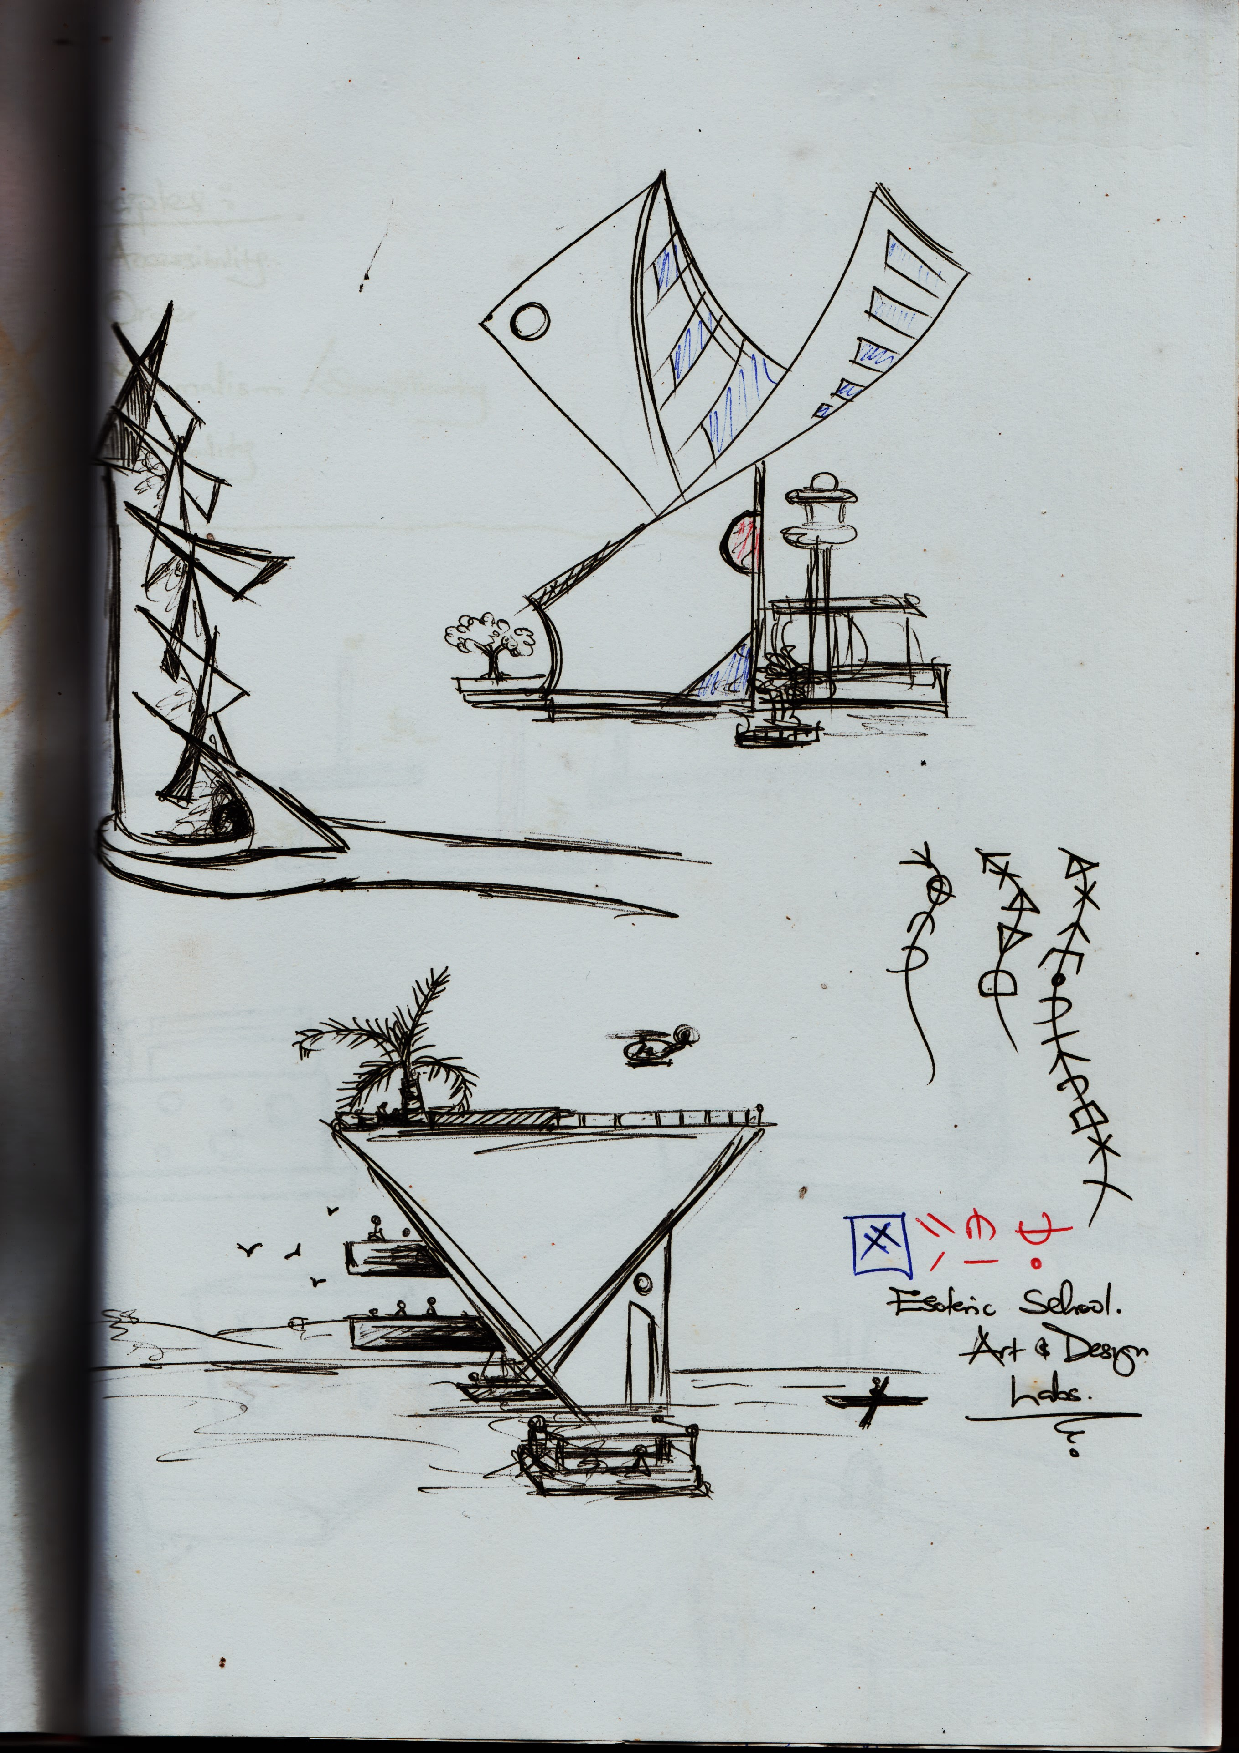
\includegraphics[trim=0cm 4cm 0cm 2.8cm, clip, width=0.9\textwidth,]{resources/pdfs/ozin_gene_expressions.pdf}\\
   \caption{An excerpt from architectural design notes by the author, from the early days of his home-based research laboratory. In this particular sketch note, we also get to see an idea similar to how gene expressions are actually a chain of glyphs that, as in the \textbf{LGES} protocols, are depicted as structures chained to each other along a \textit{backbone structure} symbolically depicted as a line (curved lines in this case). Copyrights due to author and Nuchwezi Research Labs.}
  \label{FIGCODEOZINART}
  \end{center}
\end{figure}


For some, the \textbf{Ozin Cipher}\cite{lutalo_2025_ozin} (see \textbf{\hyperref[SECOZIN]{Section \ref{SECOZIN}}}) might not seem that important or useful, but, perhaps because not everyone can immediately appreciate the fact that basic [visual and symbolic] cryptography is such a dear part of expression in nature, that whoever is the Architect of Life, has applied it abundantly throughout nature, in many creative ways --- or, cast in a different light, that when we (humans) explore nature using our creative and intellectual faculties, we find or see it vastly applied across most of nature; camouflage in reptiles and viruses, the occult languages of birds, telling, but cryptic signatures of various herbs, etc. And these phenomena have indeed inspired many observant minds throughout the ages, to pick a leaf from nature and leverage this diversity and stealthiness in expression via various ideas and in many humane fields; in mathematics and computing, in mundane as well as esoteric philosophy, and yes... in \textit{magick}! Talking of which, for those interested in getting a deeper idea concerning how such a beautiful numeric symbol system --- an alternative to the commonplace Arabic Numerals, came to be, one useful resource (and some clues) is the \textbf{CODE OGF}\cite{lutalo_2025_ogf} and a queer fascination with the \textbf{sacredness of numbers} --- especially the \texttt{kaballah} system!

\begin{figure}[H]
  \begin{center}
  %\includegraphics[trim=2cm 8cm 2cm 8cm, clip, width=0.9\textwidth,]{resources/pdfs/ProteinSynthesisStateMachine.pdf}\\
   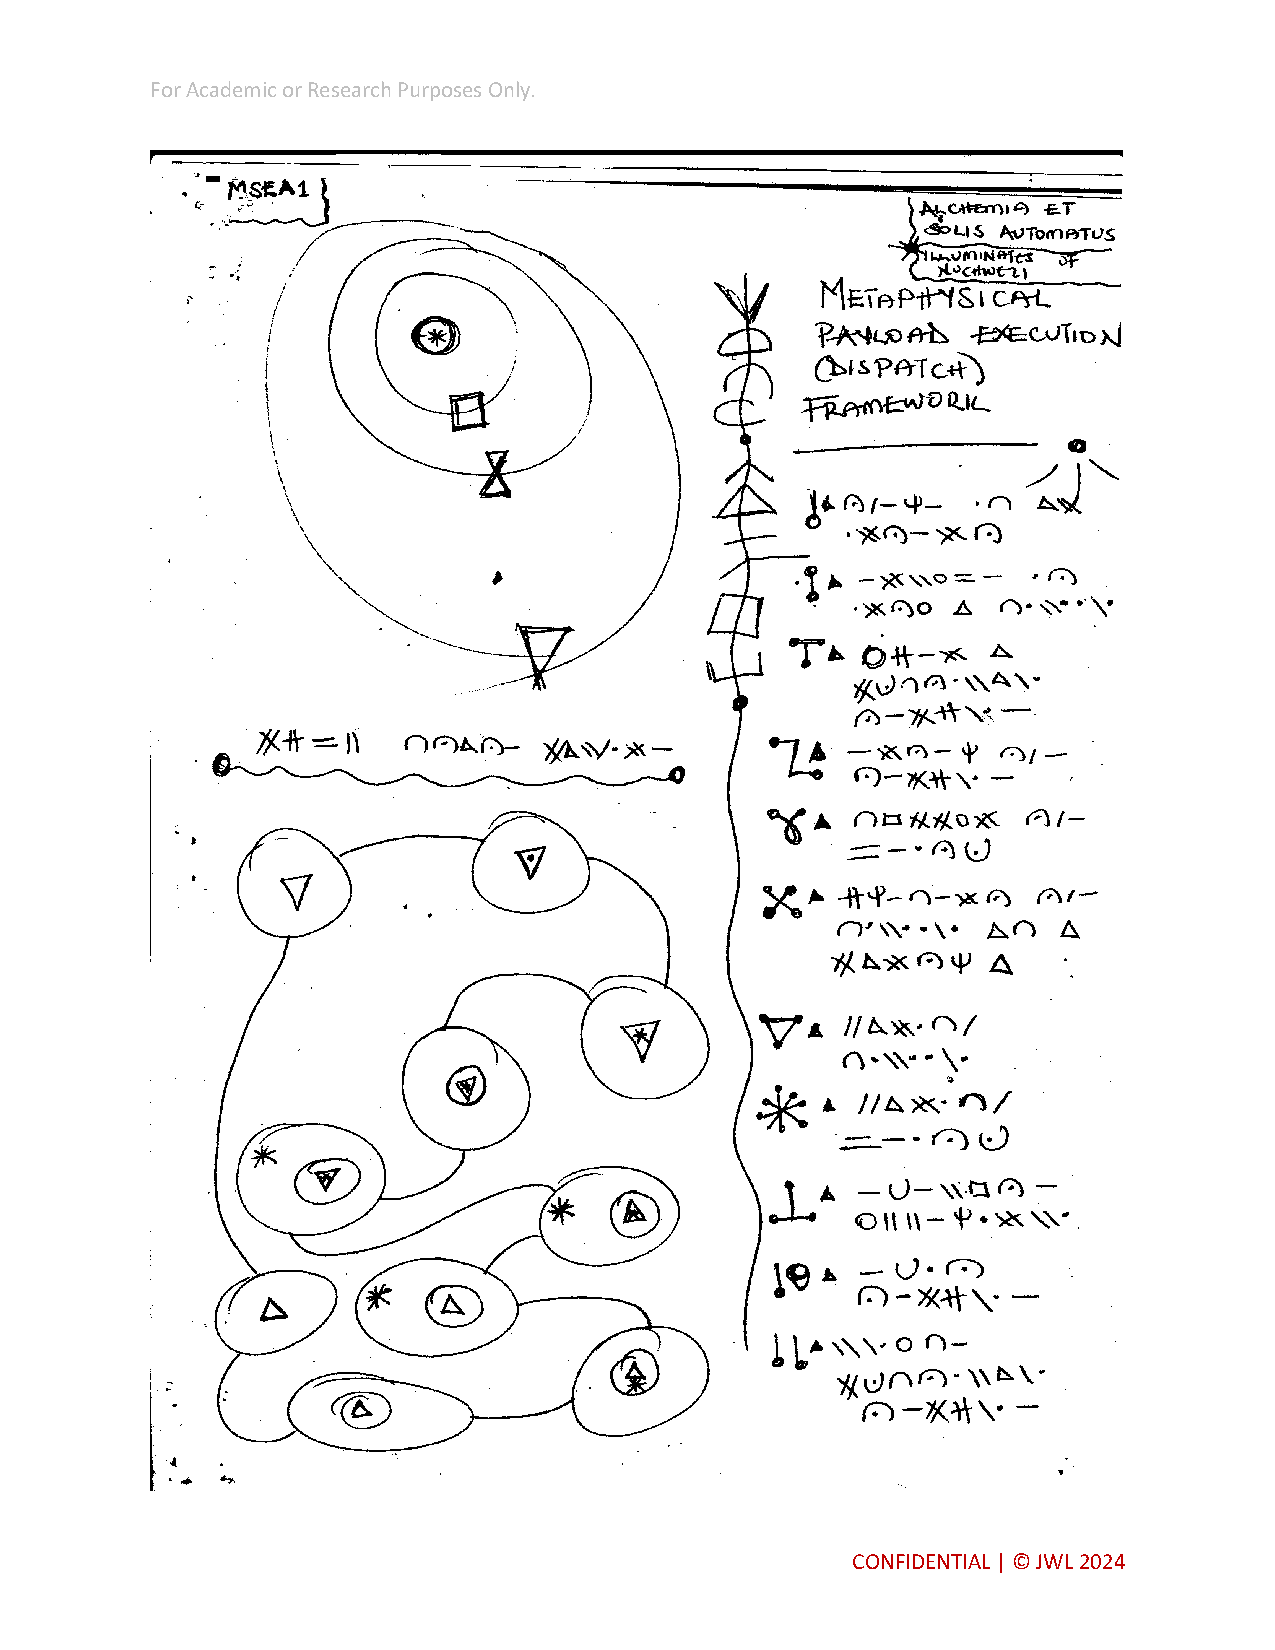
\includegraphics[trim=0cm 2cm 0cm 0cm, clip, width=0.9\textwidth,]{resources/pdfs/ozin.pdf}\\
   \caption{The OZIN Cipher in use. An excerpt from the Church of Dance Eternal OGF}
  \label{FIGCODEOZIN}
  \end{center}
\end{figure}

\textbf{\hyperref[FIGCODEOZIN]{Figure \ref{FIGCODEOZIN}}} is just an excerpt from that manuscript, perhaps not so clear because the original manuscript is handwritten\footnote{Some of these notes do have a life of their own though. So, for example, if one wishes to look at a clear scanned version of \textbf{\hyperref[FIGCODEOZINART]{Figure \ref{FIGCODEOZINART}}}, there is a copy at the author's online Art Portfolio --- \url{https://www.deviantart.com/nemesisfixx/art/Not-So-Impossible-Dwellings-823360670}, and as for \textbf{\hyperref[FIGCODEOZINNOTES]{Figure \ref{FIGCODEOZINNOTES}}}, a clear version is also curated at \url{https://www.deviantart.com/nemesisfixx/art/Nu-Druid-Calligraphy-806645934}}, and this is just a scanned version. But hopefully it drives the point home. Also, as seen from that excerpt as well as a closely related excerpt --- see \textbf{\hyperref[FIGCODEOZINNOTES]{Figure \ref{FIGCODEOZINNOTES}}}, just like we might replace numbers with alternative symbols, we also see the Latin Alphabet replaced by an ``alien-looking" hand, and this might definitely have its place in transformations of $\psi_{az}$ sequences or their expression in other ways! 


\begin{figure}[H]
  \begin{center}
  %\includegraphics[trim=2cm 8cm 2cm 8cm, clip, width=0.9\textwidth,]{resources/pdfs/ProteinSynthesisStateMachine.pdf}\\
   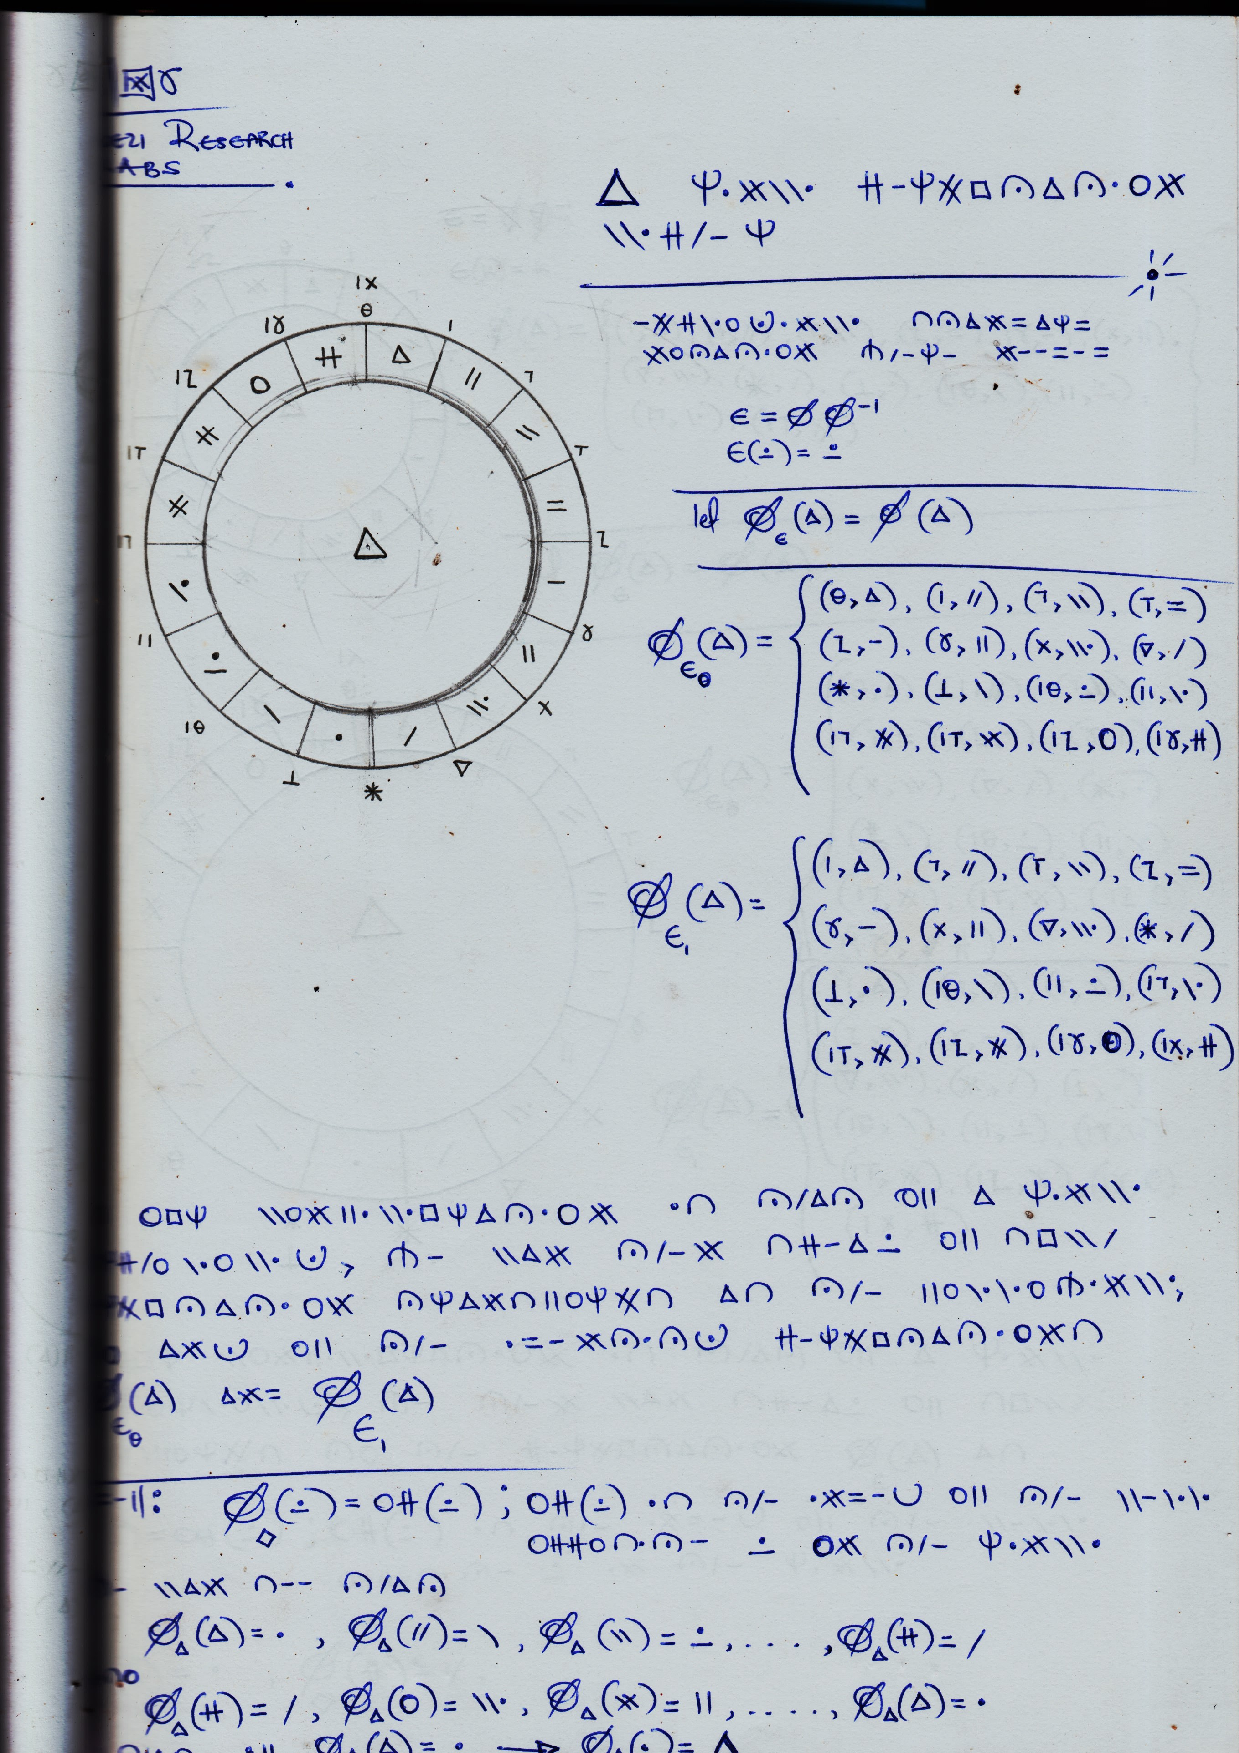
\includegraphics[ width=0.9\textwidth,]{resources/pdfs/ozin_applied.pdf}\\
   \caption{The OZIN Cipher in use. An excerpt from author's research notes (circa 2019) on developing a cryptographic system leveraging a dial mechanism. Copyrights due to author and Nuchwezi Research Labs.}
  \label{FIGCODEOZINNOTES}
  \end{center}
\end{figure}

\chapter{Computing Platonic-Form Encoding Keys (PFEKs), $\boxed{\psi_\Omega}_m$ for a Particular na-Sequence $\Theta$ and some $m$}
\label{SECIFAMSSPFMAPS}


It is one of the tricky, but otherwise readily solvable aspects of the \textbf{Lu-Genome Expression System} (LGES), that when constructing the \textbf{BODY} aspect of a \textbf{Full Genome Expression} (FGE) corresponding to a particular sequence $\Theta$, that we correctly pick or generate the corresponding platonic-form encoding key, $\boxed{\psi_\Omega}_m$, that corresponds to the sequence's characteristic, or rather, the \textbf{modal sequence}. 


In particular, we use the concept of shuffling/anagrammatizing a sequence relative to some initial/specific input \textbf{partitioning index} $k$ --- in this case, denoted $m$, and which is derived as such:

\begin{equation}
 m = \invpi(\overset{>}{\Theta})
\end{equation}\\

So that, for the case of rendering \textbf{FGE} basing on some sequence $\Theta$ --- possibly an na-Sequence, encoded (for \textbf{LGES}) using base-$\Omega$, we use the \textbf{Second Lu-Shuffle Algorithm} (SLSA) --- introduced in \textbf{\hyperref[APPSLSA]{Section \ref{APPSLSA}}}, and for which, important, example look-up-tables are shown in \textbf{\hyperref[SECAPPLYSLSA]{Section \ref{SECAPPLYSLSA}}}, to anagrammatize $\psi_\Omega$ \textbf{relative to} $m$, so as to arrive at a correct $\boxed{\psi_\Omega}_m$ that we then use to render the \textbf{PFA} for $\Theta$. Essentially, we must compute the transform:\\


\begin{trans}[Generating the \textbf{Platonic-Form Encoding Key}]
$ $\\
$\psi_\Omega \xrightarrow{slsa(\psi_\Omega, m)} \boxed{\psi_\Omega}_m$\\
\end{trans}
 
Where $slsa(\Theta,m)$ is equivalent to invoking \texttt{lu\_shuffler\_b$(\Theta,m)$} as examples in \textbf{\hyperref[LST_SLSA]{Listing \ref{LST_SLSA}}} show. 

Good enough, we not only have ready-to-use shuffled versions of $\psi_\Omega$ = $\psi_{10}$ = $\langle 0, 1, 2, 3, 4, 5, 6, 7, 8, 9 \rangle$ as shown in \textbf{\hyperref[FIGTRACESLSA]{Figure \ref{FIGTRACESLSA}}}, but also, in case one wishes to manually compute or perhaps automatically generate the necessary key for a given $m$ or \textit{any} sequence, the Python program in \textbf{\hyperref[LST_SLSA]{Listing \ref{LST_SLSA}}} can be utilized for this purpose.
 

That said, basing on the algorithm that generated the mappings in \textbf{\hyperref[FIGTRACESLSA]{Figure \ref{FIGTRACESLSA}}}, we have ready-to-use \textbf{Platonic-Form Encoding Keys} corresponding to particular values of $m$, and shuffling of $\psi_{\Omega}$ as shown in the following table.\\


 
\begin{table}[H]
  \centering
  \Large
	\begin{tabular}[t]{|p{6cm}||c|c|c|c|c|c|c|c|c|c|}
	\hline
	\multicolumn{11}{|c|}{\textbf{PFEK Look-up Table by SLSA}}\\
	\hline
	\hline
	\diagbox{$m = \invpi(\overset{>}{\Theta})$}{$I(\omega_i,\overset{>}{\Theta})$} & 1 & 2 & 3 & 4 & 5 & 6 & 7 & 8 & 9 & 10\\
	\hline
	\hline
	1 & \textbf{4} & 2 & 8 & 9 & 0 & 7 & 3 & 6 & 5 & 1\\ 
	\hline
	2 & \textbf{4} & \textbf{2} & 8 & 9 & 0 & 7 & 3 & 6 & 5 & 1\\ 
	\hline
	3 & \textbf{7} & \textbf{5} & \textbf{3} & 0 & 8 & 2 & 6 & 1 & 9 & 4\\ 
	\hline
	4 & \textbf{1} & \textbf{6} & \textbf{4} & \textbf{7} & 2 & 9 & 0 & 3 & 8 & 5\\ 
	\hline
	5 & \textbf{2} & \textbf{1} & \textbf{0} & \textbf{6} & \textbf{8} & 3 & 5 & 4 & 7 & 9\\ 
	\hline
	6 & \textbf{7} & \textbf{1} & \textbf{2} & \textbf{4} & \textbf{6} & \textbf{8} & 3 & 9 & 0 & 5\\ 
	\hline
	7 & \textbf{5} & \textbf{9} & \textbf{2} & \textbf{3} & \textbf{7} & \textbf{0} & \textbf{4} & 6 & 1 & 8\\ 
	\hline
	8 & \textbf{9} & \textbf{1} & \textbf{5} & \textbf{4} & \textbf{3} & \textbf{2} & \textbf{7} & \textbf{8} & 6 & 0\\ 
	\hline
	9 & \textbf{5} & \textbf{6} & \textbf{3} & \textbf{9} & \textbf{0} & \textbf{4} & \textbf{2} & \textbf{7} & \textbf{1} & 8\\ 
	\hline
	10 & \textbf{6} & \textbf{3} & \textbf{8} & \textbf{2} & \textbf{1} & \textbf{9} & \textbf{7} & \textbf{4} & \textbf{0} & \textbf{5}\\
	              \hline
\end{tabular}
 \caption{Platonic Form Encoding Keys (PFEK) mapped to corresponding values of $m = \invpi(\overset{>}{\Theta})$ using \textbf{SLSA}}
  \label{TABSSLAPERK}
\end{table}


And if one wishes to render their \textbf{PFA} --- the platonic form aspect, of the \textbf{FGE} using the \textbf{FLSA}, then the corresponding table would be as follows:\\


\begin{table}[H]
  \centering
  \Large
	\begin{tabular}[t]{|p{6cm}||c|c|c|c|c|c|c|c|c|c|}
	\hline
	\multicolumn{11}{|c|}{\textbf{PFEK Look-up Table by FLSA}}\\
	\hline
	\hline
	\diagbox{$m = \invpi(\overset{>}{\Theta})$}{$I(\omega_i,\overset{>}{\Theta})$} & 1 & 2 & 3 & 4 & 5 & 6 & 7 & 8 & 9 & 10\\
	\hline
	\hline
	1 & \textbf{9} & 7 & 4 & 0 & 5 & 3 & 8 & 2 & 1 & 6\\ 
	\hline 
	2 & \textbf{9} & \textbf{7} & 4 & 0 & 5 & 3 & 8 & 2 & 1 & 6\\ 
	\hline 
	3 & \textbf{8} & \textbf{6} & \textbf{3} & 9 & 4 & 2 & 7 & 1 & 0 & 5\\ 
	\hline 
	4 & \textbf{8} & \textbf{6} & \textbf{3} & \textbf{9} & 4 & 2 & 7 & 0 & 1 & 5\\
	\hline
	5 & \textbf{5} & \textbf{3} & \textbf{0} & \textbf{6} & \textbf{1} & 7 & 4 & 8 & 9 & 2\\
	\hline
	6 & \textbf{5} & \textbf{1} & \textbf{2} & \textbf{6} & \textbf{3} & \textbf{7} & 4 & 8 & 9 & 0\\
	\hline 
	7 & \textbf{0} & \textbf{8} & \textbf{9} & \textbf{1} & \textbf{5} & \textbf{2} & \textbf{6} & 3 & 4 & 7\\
	\hline 
	8 & \textbf{3} & \textbf{8} & \textbf{9} & \textbf{4} & \textbf{2} & \textbf{5} & \textbf{6} & \textbf{0} & 1 & 7\\
	\hline
	9 & \textbf{9} & \textbf{1} & \textbf{2} & \textbf{3} & \textbf{8} & \textbf{4} & \textbf{5} & \textbf{6} & \textbf{7} & 0\\ 
	\hline
	10 & \textbf{9} & \textbf{5} & \textbf{6} & \textbf{7} & \textbf{8} & \textbf{0} & \textbf{1} & \textbf{2} & \textbf{3} & \textbf{4}\\
	\hline
	              
\end{tabular}
 \caption{Platonic Form Encoding Keys (PFEK) mapped to corresponding values of $m = \invpi(\overset{>}{\Theta})$ using \textbf{FLSA}}
  \label{TABFSLAPERK}
\end{table}


However, having the \textbf{PFEK} tables is one thing, while, knowing what to use them for, or how to use them is another, and we cover the gist of that, under the next title.


\subsection{Example of Resolving PFA Components, $\boxed{\omega_i^*}$}

We shall not attempt to render a complete \textbf{FGE} here since that matter is already well catered for in the associated chapter and section --- see \textbf{\hyperref[SECFULLGES]{Section \ref{SECFULLGES}}}. However, we shall attempt to set straight, the necessary procedures for:

\begin{enumerate}
\item{Computing $m$ for a given $\Omega$-encoded sequence $\Theta$:

\begin{enumerate}
\item Compute the \textbf{modal sequence statistic}, $\overset{>}{\Theta}$ --- see \textbf{Definition 1} in \cite{transformatics}.
\item Compute $m$ from the cardinality of the modal sequence as: $m = \invpi(\overset{>}{\Theta})$.
\end{enumerate}
}
\item {Picking the correct \textbf{PFEK} for that $m$ --- i.e. $\boxed{\psi_{pf}}_m$:
	\begin{enumerate}
	\item If using \textbf{FLSA}, refer to \textbf{\hyperref[TABFSLAPERK]{Table \ref{TABFSLAPERK}}}, and for any $m = k$, pick the row for which the first column has the value $k$.
	\item Of course, for any $m = k$, the only useful values on that row for doing the \textbf{PFEK} operations are the \textbf{first $k$ emboldened} values on the row corresponding to $m$. E.g. for $m=2$ the necessary key is just $\langle 9, 7 \rangle$, not the entire row.
	\item If using \textbf{SLSA}, lookup the \textbf{PFEK} using \textbf{\hyperref[TABSSLAPERK]{Table \ref{TABSSLAPERK}}}, so that, for $m = 2$, we have $\boxed{\psi_{pf}}_2 = \langle 4, 2 \rangle $
	\end{enumerate}
}
\item{ Resolving the correct component from $\boxed{\psi_{pf}}_m$ corresponding to a particular element $\omega_i$ in the corresponding \textbf{IFA MSS}, $\overset{>}{\Theta}$.
\begin{enumerate}
    \item So, if our \textbf{IFA MSS} was just $\langle 0, 2, 1, 3, 6 \rangle$ such as for $\Omega_{3}$ from \textbf{\hyperref[EQDNEXA]{Equation \ref{EQDNEXA}}}, then, taking note of the special case for any $\omega_i^* = 0$ --- such as the first term in this case (see \textbf{Step\#2(e)ii} in \textbf{\hyperref[ALGCOZINPLATO]{Algorithm \ref{ALGCOZINPLATO}}}), we merely map values of `0' in the \textbf{MSS} to just the \textbf{JOINT/GAP} element in \textbf{\hyperref[FIGPLATONICCIPH]{Figure \ref{FIGPLATONICCIPH}}}), and for the other terms, such as $\omega_3^* = 3$, since the corresponding \textbf{PFEK} for $m=5$ is $\boxed{\psi_{pf}}_5 = \langle 2, 1, 0, 6, 8 \rangle $, then $\boxed{\omega_3^*} = 0$ as per the corresponding look-up mapping we see for such an \textbf{MSS}:


\[
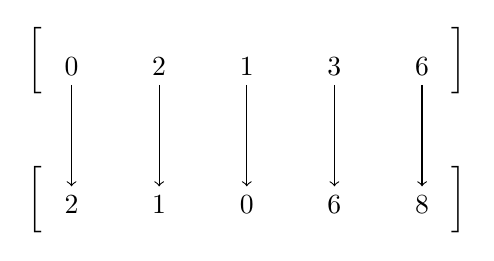
\begin{tikzpicture}[baseline=(current bounding box.center)]
  % Matrix A
  \matrix (A) [matrix of math nodes, left delimiter={[}, right delimiter={]}, row sep=1em, column sep=2em] {
    0 & 2 & 1 & 3 & 6 \\
  };

  % Matrix B
  \matrix (B) [matrix of math nodes, left delimiter={[}, right delimiter={]}, row sep=1em, column sep=2em, below=3em of A] {
    2 & 1 & 0 & 6 & 8\\
  };

  % Draw arrows from A_i to B_i
  \foreach \i in {1,2,3,4,5}
    \draw[->] (A-1-\i) -- (B-1-\i);
\end{tikzpicture}
\]

And so, for the last term in that \textbf{MSS}, $\boxed{\omega_5^*} = 8$

\end{enumerate}
}

\item{How to render the final pf-encoded version of $\omega_i^*$, i.e. $\boxed{\omega_i^*}$?
\begin{enumerate}
\item So, now that you know the \textbf{PFEK} for your $m$, such as $\boxed{\psi_{pf}}_5 = \langle 2, 1, 0, 6, 8 \rangle $ from above, and have the correct pf-term for a particular term in the \textbf{MSS} such as $\boxed{\omega_5^*} = 8$ in the example above, the corresponding pf-term is the platonic structure from \textbf{\hyperref[FIGPLATONICCIPH]{Figure \ref{FIGPLATONICCIPH}}} that corresponds to the index $8$ --- so that would be the \textbf{octagon} or rather \textbf{octa-gram} with nothing at the center. But also, given the term we are decoding is $\omega_5^*$ = 6, then the overall structure would be as per configuration \textbf{$8_{pf} + 8 \times 6_{oz}$}: That is to say:

\begin{equation}
\boxed{\omega_5^*}_{pf} = 8_{pf} \otimes 6_{oz} = 8_{pf} + 8 \times 6_{oz}
\end{equation}

So that the final rendered term for this element alone would be as shown:


\begin{figure}[H]
  \begin{center}
   %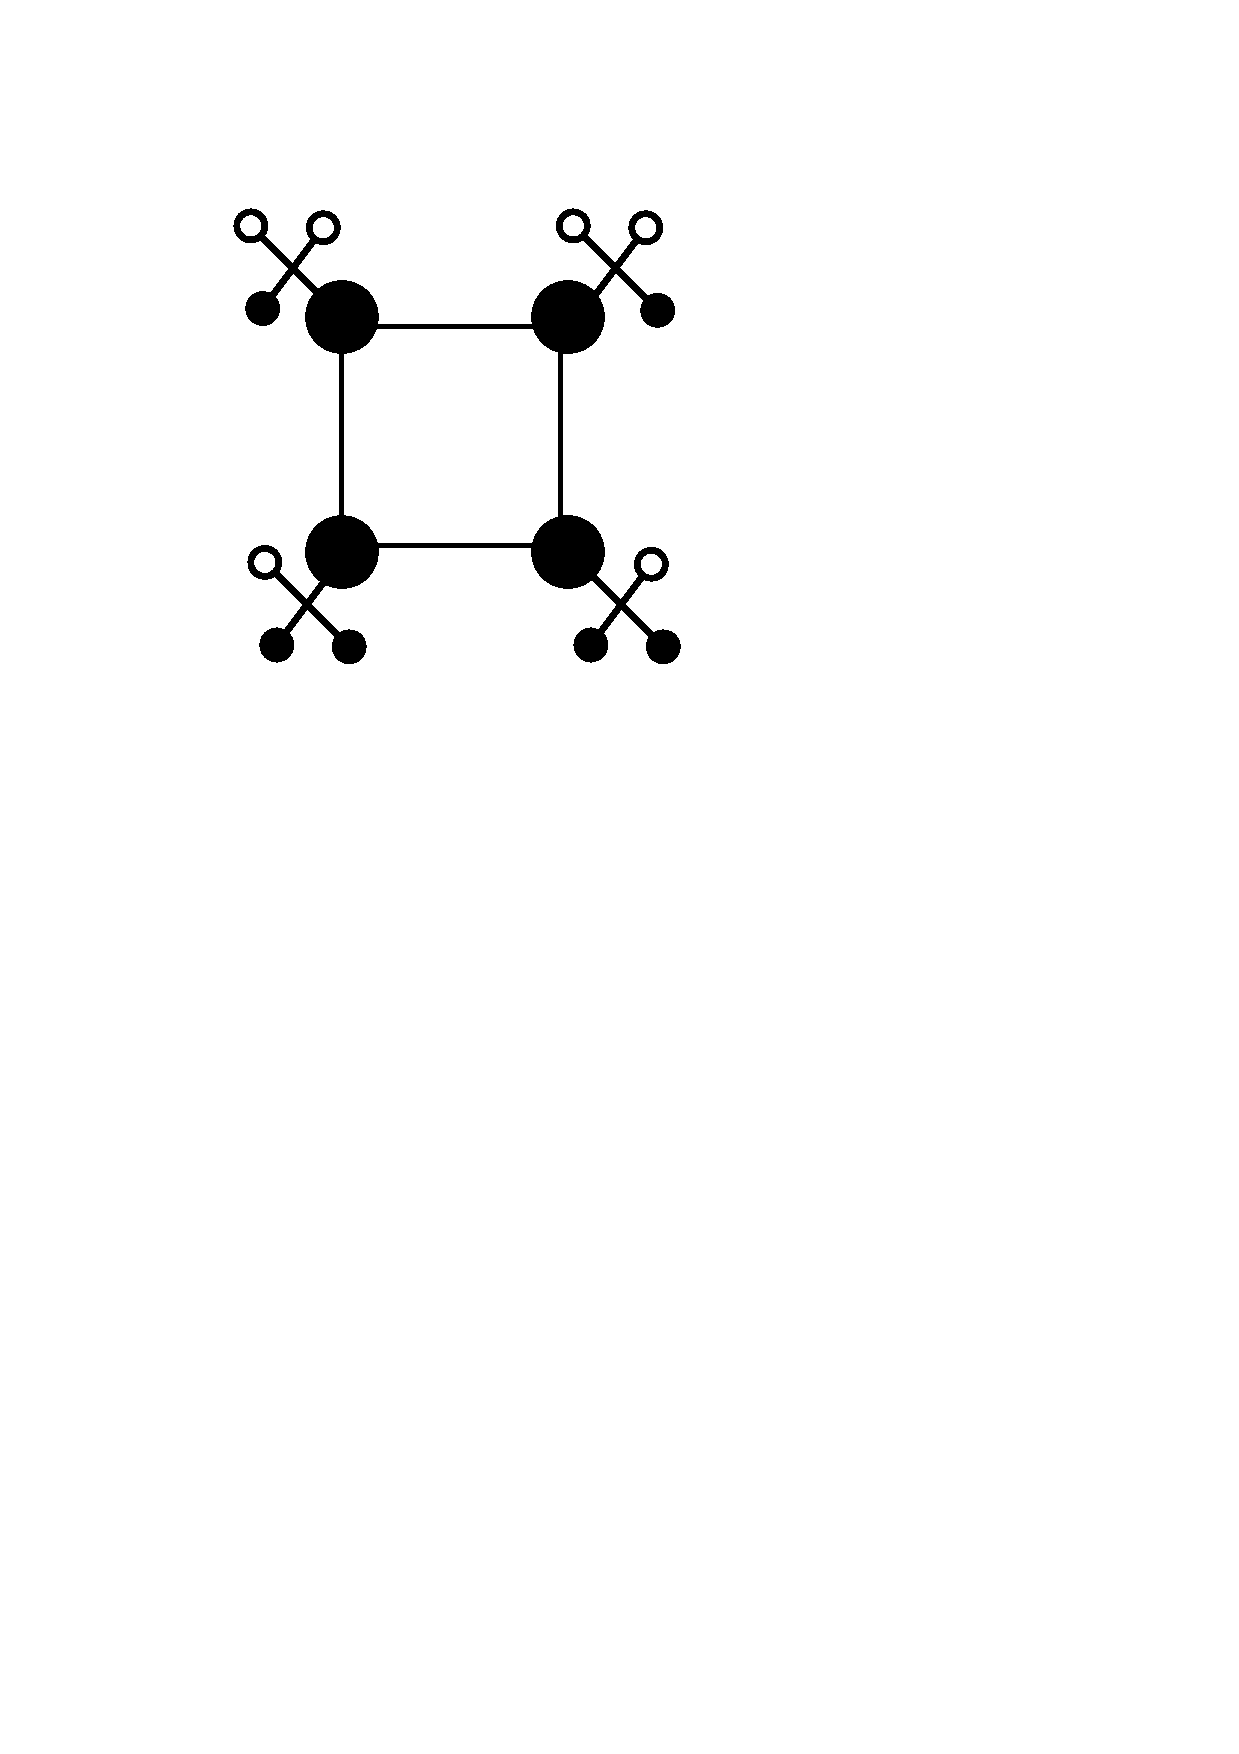
\includegraphics[trim=LEFT BOTTOM RIGHT TOP, clip, width=0.9\textwidth,]{resources/pdfs/EXAPLATONICFORM-PFA.pdf}\\
   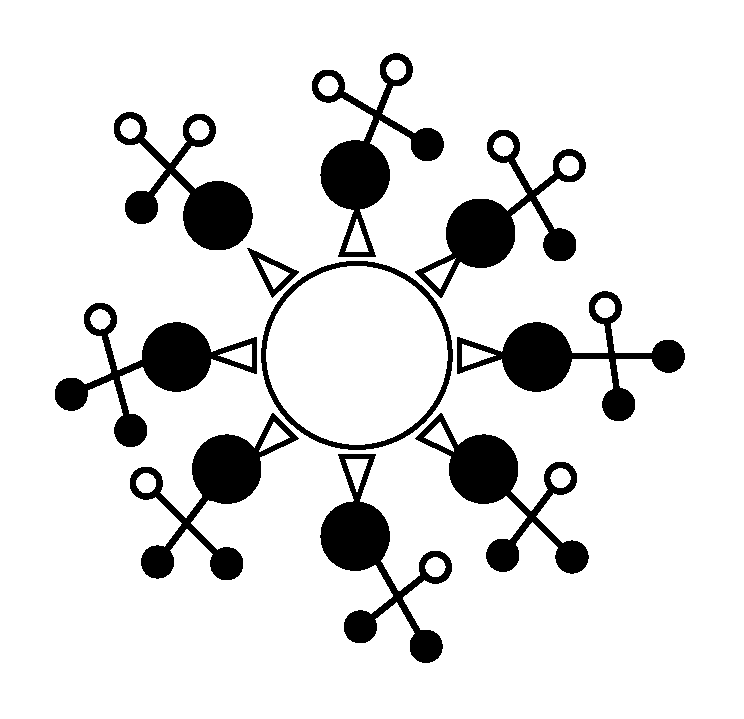
\includegraphics[ width=0.9\textwidth,]{resources/pdfs/EXAPLATONICFORMPFA_OCT.pdf}\\
   \caption{An example of a single \textbf{PFA} component equivalent to the configuration \textbf{$8_{pf} \otimes 6_{oz}$}.}
  \label{FIGEXAPLATONICFORMPFA_OCT}
  \end{center}
\end{figure}



\end{enumerate}
}
\end{enumerate}

Of course, once one has the correct $\boxed{\omega_i^*}$, they can just attach it to the existing \textbf{FGE} chain-structure so as to advance the piece-wise construction the complete \textbf{BODY} aspect of a full genome expression for $\Theta$.




\chapter{Alternative[ORIGINAL] $\Omega$-to-PLATONIC Form Genetic Code Expression Algorithm}
\label{SECALTPFGESA}

While developing the theory for the \textbf{Lu-Genome Expression System}, and particularly while and after looking at the way the original concept of the algorithm for generating the BODY-components of the \textbf{FGE} was working --- for example, it uses the \textbf{IFA MSS} as key to pick corresponding platonic form structures from $\lnot(\psi_{pf})$ and not directly from $\psi_{pf}$ --- because, the idea was that, the most frequent term in the \textbf{IFA MSS} should correspond to a \textit{larger} or \textit{more prominent} or \textit{more complex} geometric form than the least significant terms. And thus, we shall see that, since natural genetic sequences (or rather, DNA-sequences) only span $\psi_{DNA}$ which has only 4 distinct symbols, then we would never have a meaningful way to utilize the complete set of 10 distinct geometrical structures from $\psi_{pf}$. 


That last observation is one of the interesting consequences of \textbf{\hyperref[ALGCOZINPLATO_ORIG]{Algorithm \ref{ALGCOZINPLATO_ORIG}}} (particularly \textbf{\hyperref[EQFBOXED_ORIG]{Equation \ref{EQFBOXED_ORIG}}}) that performs the translation from \textbf{mRNA}-equivalent $\Omega$-encoded \textbf{IFA MSS} to geometric $pf$-encoded \textbf{PFA}, using the $\lnot(\psi_{pf})$. We find that (\textbf{irrespective} of the organism or species we would look at) it seems as though the resulting \textbf{PFA} expressions \textbf{must} always \textbf{only} utilize the \textbf{first four} elements of $\lnot(\psi_{pf})$ --- $\langle 9, 8, 7, 6 \rangle$, since all possible \textbf{IFA MSS} would only have at most, $4$ distinct symbols in them. And if we had not used $\lnot(\psi_{pf})$, still, a direct use of $\psi_{pf}$ would only utilize the start of that symbol set if we map elements in $\psi_{DNA}$ to those in $\psi_{pf}$ (even via $\psi_\Omega$ as we do in \textbf{\hyperref[TRANSSEQATG]{Transformation \ref{TRANSSEQATG}}}), thus why we returned to the drawing board, and developed \textbf{\hyperref[ALGCOZINPLATO]{Algorithm \ref{ALGCOZINPLATO}}} instead.

Studying the resulting genome expressions visually, one would find that it seems like we always express the BODY of any \textbf{FGE} with some structure containing a \textbf{nucleus}\footnote{Of course, the way the platonic forms corresponding to \textbf{9} and \textbf{7} were simplified to those of \textbf{8} (octagon-\textit{chaosstar}-octagram) and \textbf{6}(hexagon-\textit{hexagram}) respectively, with \textbf{the twist} that the \textbf{extra appendage point is placed at the center of the geometric structure instead of creating an extra vertex/appendage point} does have some good justification though --- \textit{\textbf{Occam's Razor} principle in a way, but also that, while observing nature, we typically find that \textbf{Simple is Better}}. Nonetheless, the sensibilities of mapping any $i$ in $\psi_{10}$ or rather $\psi_\Omega$ to a platonic form corresponding to \textbf{the regular polygon with each internal angle} corresponding to $\frac{360}{i}$ still makes sense for all 10 terms in $\psi_\Omega$.}\footnote{The inverse would be \textbf{BODY} made of mostly gaps or joints, basic linear structures and triangles!}!

We shall keep that original algorithm here, for mostly study/comparison purposes...

\begin{alg}[The \textbf{$\Omega$-to-PLATONIC Form Genetic Code Expression Algorithm}]
\label{ALGCOZINPLATO_ORIG}

Assuming we have an $\Omega$-base encoded genetic code sequence $\Theta_\Omega$ of some length $n > 0$.

\begin{enumerate}
    \item{Initialize the expression with a transcription, by Using \textbf{\hyperref[ALGCOZIN]{Algorithm \ref{ALGCOZIN}}} to construct the \textbf{Intermediate Form Affix} (IFA) of $\Theta_\Omega$ --- essentially return $OZ(\Theta_\Omega)$ as the start of the \textbf{Final Genome Expression} (FGE) $\boxed{OZ(\Theta_\Omega)}^*$ --- so that the final complete expressed(transcribed+translated ) sequence shall be as:\\

\begin{equation}
\label{EQTRANSLGENSEQ_ORIG}
\boxed{OZ(\Theta_\Omega)}^* = OZ(\Theta_\Omega)\cdot\boxed{OZ(\Theta_\Omega)}
\end{equation}\\

$\boxed{OZ(\Theta_\Omega)}: \mathbb{N} \times \psi_{pf}$ is the suffix of expressed na-Sequence $\Theta_\Omega$, and is expressed in our genome expression system, as PLATONIC-Form encoded \textbf{modal sequence statistic} of $OZ(\Theta_\Omega)$\footnote{We render the \textbf{suffix of FGE} as $\overset{>}{OZ(\Theta_\Omega)}$ because it allows us to not express $\Theta_\Omega$ naively at the genome or gene level, but also, so that, from an information-theoretic perspective, the completed genome expression is somewhat a statistical summary of what the genome sequence contains --- the appearance of an animal or a plant or virus, depicting or expressing the summary of its DNA code. We do this then, by not merely doing a 1-to-1 translation of the intermediate Ozin-code expression $OZ(\Theta_\Omega)$, but instead computing its summary in form of $\overset{>}{OZ(\Theta_\Omega)}$, and then instead translating that into the final spatial/geometric forms as per $\psi_{pf}$. This shall then help complete the entire processing/synthesis of sequence $\Theta_\Omega$, or rather our genome expression.} --- the \textbf{PFA}\footnote{Platonic Form Aspect}, i.e.:\\

\begin{equation}
 \boxed{OZ(\Theta_\Omega)} = \boxed{\overset{>}{OZ(\Theta_\Omega)}}_{pf}
\end{equation}\\


}
\item{ So once we have the \textbf{IFA}, $OZ(\Theta_\Omega)$, proceed to use it to generate the rest of the sequence expression as follows: 
\begin{enumerate}
\item {\textbf{INITIALIZE} FGE, $\boxed{OZ(\Theta_\Omega)}^*$ as just:\\

\begin{equation}
\label{EQSTARTFGE_ORIG}
\boxed{OZ(\Theta_\Omega)}^* = \langle \langle OZ(\Theta_\Omega) \rangle \langle \rangle \rangle
\end{equation}\\

This ensures, we have the prefix affix, \textbf{IFA}, as the contents of the sequence start of \textbf{FGE} \textit{extended} by a \textbf{still empty subsequence} --- in expression form, this shall merely be a backbone structure with \textbf{IFA} as its head, and a terminal that is ready to have more units appended to it, \textbf{after a single GAP/JOINT extension to IFA}. So, it also means, at this juncture, \textbf{PFA} is just:\\

\begin{equation}
\label{EQSTARTFGESUF_ORIG}
\boxed{OZ(\Theta_\Omega)} = \langle \rangle
\end{equation}\\

}
\item {
	\textbf{COMPUTE} the \textbf{IFA MSS}, $\overset{>}{OZ(\Theta_\Omega)}$
}
\item{\textbf{FOREACH} symbol/term $\omega_i^*$ in \textbf{IFA MSS}, $\overset{>}{OZ(\Theta_\Omega)}$: 
\begin{enumerate}
    \item{\textbf{USE} the translation mapping: $\psi_\Omega \rightarrow \lnot(\psi_{pf}) \rightarrow \psi_{pf}$ as depicted in \textbf{\hyperref[FIGPLATONICCIPH]{Figure \ref{FIGPLATONICCIPH}}}, to translate $\omega_i^*$ into the equivalent \textbf{Platonic Form}, $\boxed{\omega_i^*}$ for the final code as such:}
\item { \textbf{IF} $\omega_i^* \equiv 0$:Operating on the current \textbf{FGE}: 
		\begin{enumerate}
		\item { Append/Insert a JOINT onto \textbf{FGE},  $\boxed{OZ(\Theta_\Omega)}^*$

		\begin{equation}
		\label{EQEXTFGEJOINT_ORIG}
		\boxed{OZ(\Theta_\Omega)}^* = \boxed{OZ(\Theta_\Omega)}^* \cdot \boxed{\omega_i^*}_{joint}
		\end{equation}		
		
		And equivalently:
		
		\begin{equation}
		\label{EQEXTFGEJOINTSUF_ORIG}
		\boxed{OZ(\Theta_\Omega)} = \boxed{OZ(\Theta_\Omega)} \cdot \boxed{\omega_i^*}_{joint}
		\end{equation}				
		
		}
		\item \textbf{PROCEED} to the next symbol in \textbf{IFA MSS}, $\overset{>}{OZ(\Theta_\Omega)}$\\ (loop from \textbf{Step\#2(c))}.
		\end{enumerate}
	}
	\item { \textbf{ELSE}: \textbf{resolve} the correct  $\boxed{\omega_i^*}$  for  $\omega_i^*$  by using the relation:\\

\begin{equation}
\label{EQFBOXED_ORIG}
 \boxed{\omega_i^*} = \rho_j +  j \times \omega_i^* : j = I(\rho_j,\lnot(\psi_{pl})) = I(\omega_i^*,\psi_\Omega)
\end{equation}\\

	\begin{enumerate}
        \item{\textbf{PLACE} that encoded version, $\boxed{\omega_i^*}$, along the existing \textbf{FGE} structure at the next vacant position ($\invpi(\Theta_\Omega)+i$). Expressible with another version of \textbf{\hyperref[EQEXTFGEJOINT_ORIG]{Equation \ref{EQEXTFGEJOINT_ORIG}}} as:
	
	\begin{equation}
	\label{EQEXTFGEPF_ORIG}
		\boxed{OZ(\Theta_\Omega)}^* = \boxed{OZ(\Theta_\Omega)}^* \cdot \boxed{\omega_i^*}
		\end{equation}	
		
		And equivalently:
		
		\begin{equation}
		\label{EQEXTFGEPFSUF_ORIG}
		\boxed{OZ(\Theta_\Omega)} = \boxed{OZ(\Theta_\Omega)} \cdot \boxed{\omega_i^*}
		\end{equation}	
		
            Where the special term, $\boxed{\omega_i^*}$, as per \textbf{\hyperref[EQFBOXED_ORIG]{Equation \ref{EQFBOXED_ORIG}}}, is basically the PLATONIC Form corresponding to position $j$ in $\lnot(\psi_{pf})$ --- a \textbf{complement/inverted symbol set}, thus one of the final form platonic geometry structures, but also with the intermediate form $\omega_i^*$ expressed $j$ times as an attachment to $\rho_j$, such that:\\
	
	\begin{equation}
	0 \leq (j = (\invpi(\psi_{pf})-i)) \leq (\invpi(\psi_{pf}) = \invpi(\psi_\Omega)) \geq \invpi(\overset{>}{OZ(\Theta_\Omega)})
	\end{equation}\\
	
	
            as depicted in example \textbf{\hyperref[FIGEXAPLATONICFORMPFA]{Figure \ref{FIGEXAPLATONICFORMPFA}}}, with each expression of $\omega_i^*$ attached to one of the $j$ \textbf{appendage spots} on the shape for $\boxed{\omega_i^*}$.
	}
	\item \textbf{PROCEED} to the next symbol in \textbf{IFA MSS}, $\overset{>}{OZ(\Theta_\Omega)}$\\ (loop from \textbf{Step\#2(c))}.
	\end{enumerate}
	}
\end{enumerate}
}
\end{enumerate}
}

\item \textbf{TRUNCATE} the final-structure after the final term in \textbf{FGE}.
\item \textbf{RETURN} \textbf{FGE}, $\boxed{OZ(\Theta_\Omega)}^*$ as the final transcribed and translated version of $\Theta_\Omega$. The culmination of our conceptual genome expression.
\end{enumerate}
$\qed$
\end{alg}


\vspace{2em}
\begin{center}
\fbox{\begin{minipage}{0.9\textwidth}
\large
\textbf{NOTE:}\\
 
Besides the introductory notes about this alternative algorithm given at the start of this appendix chapter, it might be worth the effort, looking at what kinds of expressions the algorithm can produce, so one has a basic means to weigh it against the version we prefer/chose (\textbf{\hyperref[ALGCOZINPLATO]{Algorithm \ref{ALGCOZINPLATO}}} in \textbf{\hyperref[SECGENSEQEXPRES]{Section \ref{SECGENSEQEXPRES}}}). Thus, without delving much into how they were generated, we shall [re-]iterate some of the highlights of how \textbf{\hyperref[ALGCOZINPLATO_ORIG]{Algorithm \ref{ALGCOZINPLATO_ORIG}}} would render various sequences under the \textbf{Lu-Genome Expression System}.

\end{minipage}}
\\
\end{center}
\vspace{2em}


\textbf{IMPORTANT:} Realize that \textbf{Step\#2(c)iii(A)} of \textbf{\hyperref[ALGCOZINPLATO_ORIG]{Algorithm \ref{ALGCOZINPLATO_ORIG}}} processes/operates on the \textbf{IFA MSS}, $\overset{>}{OZ(\Theta_\Omega)}$, and not the \textbf{IFA} directly. This, so that, first, we don't process multiple times any term or symbol from the \textbf{IFA}\footnote{Which is a direct translation of the genetic code.} in the \textbf{PFA}. And then also, the way the translation works, is that if $\omega_x^* > \omega_y^*$ or rather that $|\omega_x^*| > |\omega_y^*|$,  then $\omega_x^*$ shall correspond to a term in $\lnot(\psi_{pf})$ that is simpler\footnote{The idea was somewhat to assign more complex forms to terms in the associated symbol set that occur earlier than others, since it somewhat depicts their relative higher significance --- a concept similar to how we would attempt to regenerate a sequence from its modal sequence statistic without say consulting its sequence characteristic --- an inversion of and adaptation of the \textbf{string chart} concept first presented in the \textbf{LOMT-1 Transformer} (\textbf{Transformer 6} in \cite{transformatics}).} in form than $\omega_y^*$ --- higher significance being assigned to earlier-occurrence in the underlying symbol set $\psi_\Omega$. 


Good enough, we have already treated of sequence complements and inverted look-ups in \textbf{\hyperref[SECSIGCOMPLE]{Section \ref{SECSIGCOMPLE}}}, and so, for this case, the corresponding mapping from terms (or rather, magnitudes) in $\overset{>}{OZ(\Theta_\Omega)}$ to indices in  $\lnot(\psi_{pf})$ is as below --- also stressing the fact that $0 \leq |\omega_i^*| = |\omega_i| < \invpi(\psi_{pf})$ for all $\omega_i \in \Theta_\Omega \quad \land \quad \omega_i^* \in \overset{>}{\Theta_\Omega}$.


\[
\begin{tikzpicture}[baseline=(current bounding box.center)]
  % Matrix A
  \matrix (A) [matrix of math nodes, left delimiter={[}, right delimiter={]}, row sep=1em, column sep=2em] {
    0 & 1 & 2 & 3 & 4 & 5 & 6 & 7 & 8 & 9\\
  };

  % Matrix B
  \matrix (B) [matrix of math nodes, left delimiter={[}, right delimiter={]}, row sep=1em, column sep=2em, below=3em of A] {
    9 & 8 & 7 & 6 & 5 & 4 & 3 & 2 & 1 & 0\\
  };

  % Draw arrows from A_i to B_i
  \foreach \i in {1,2,3,4,5,6,7,8,9,10}
    \draw[->] (A-1-\i) -- (B-1-\i);
\end{tikzpicture}
\]

Looking at some example genome expressions rendered using \textbf{\hyperref[ALGCOZINPLATO_ORIG]{Algorithm \ref{ALGCOZINPLATO_ORIG}}} shall help most reviewers to appreciate whether or not it is better or worse than \textbf{\hyperref[ALGCOZINPLATO]{Algorithm \ref{ALGCOZINPLATO}}}, and whether or not it is better at representing how natural genome expression occurs as seen in our inspiration case --- see \textbf{\hyperref[FIGPINEAPPLE]{Figure \ref{FIGPINEAPPLE}}}.

\subsection{Examples of Complete Lu-Genome Expressions}
\label{SECFULLGES_ORIG}

We get to see the first example of the output of processing some na-Sequence expressed originally in base-$\Omega$ such as for $\Omega_{3}$ from \textbf{\hyperref[EQDNEXA]{Equation \ref{EQDNEXA}}}, in its final expression form as in \textbf{\hyperref[FIGPLATONICEXA_ORIG]{Figure \ref{FIGPLATONICEXA_ORIG}}}\cite{lutalo_2025_exa} --- more importantly, since we have already seen its \textbf{IFA} (the \textbf{FGE} prefix) in \textbf{\hyperref[FIGOZEXA]{Figure \ref{FIGOZEXA}}}, we note that, we essentially see the update as the result of expressing the entire \textbf{FGE} via the \textbf{IFA MSS} equivalent to:

\begin{equation}
\overset{>}{\Omega_{3}} = \langle 0, 2, 1, 3, 6 \rangle \implies \boxed{OZ(\Omega_{3})} \approx \langle GAP, 7, 8, 6, 3 \rangle
\end{equation}


\begin{figure}[H]
  \begin{center}
  %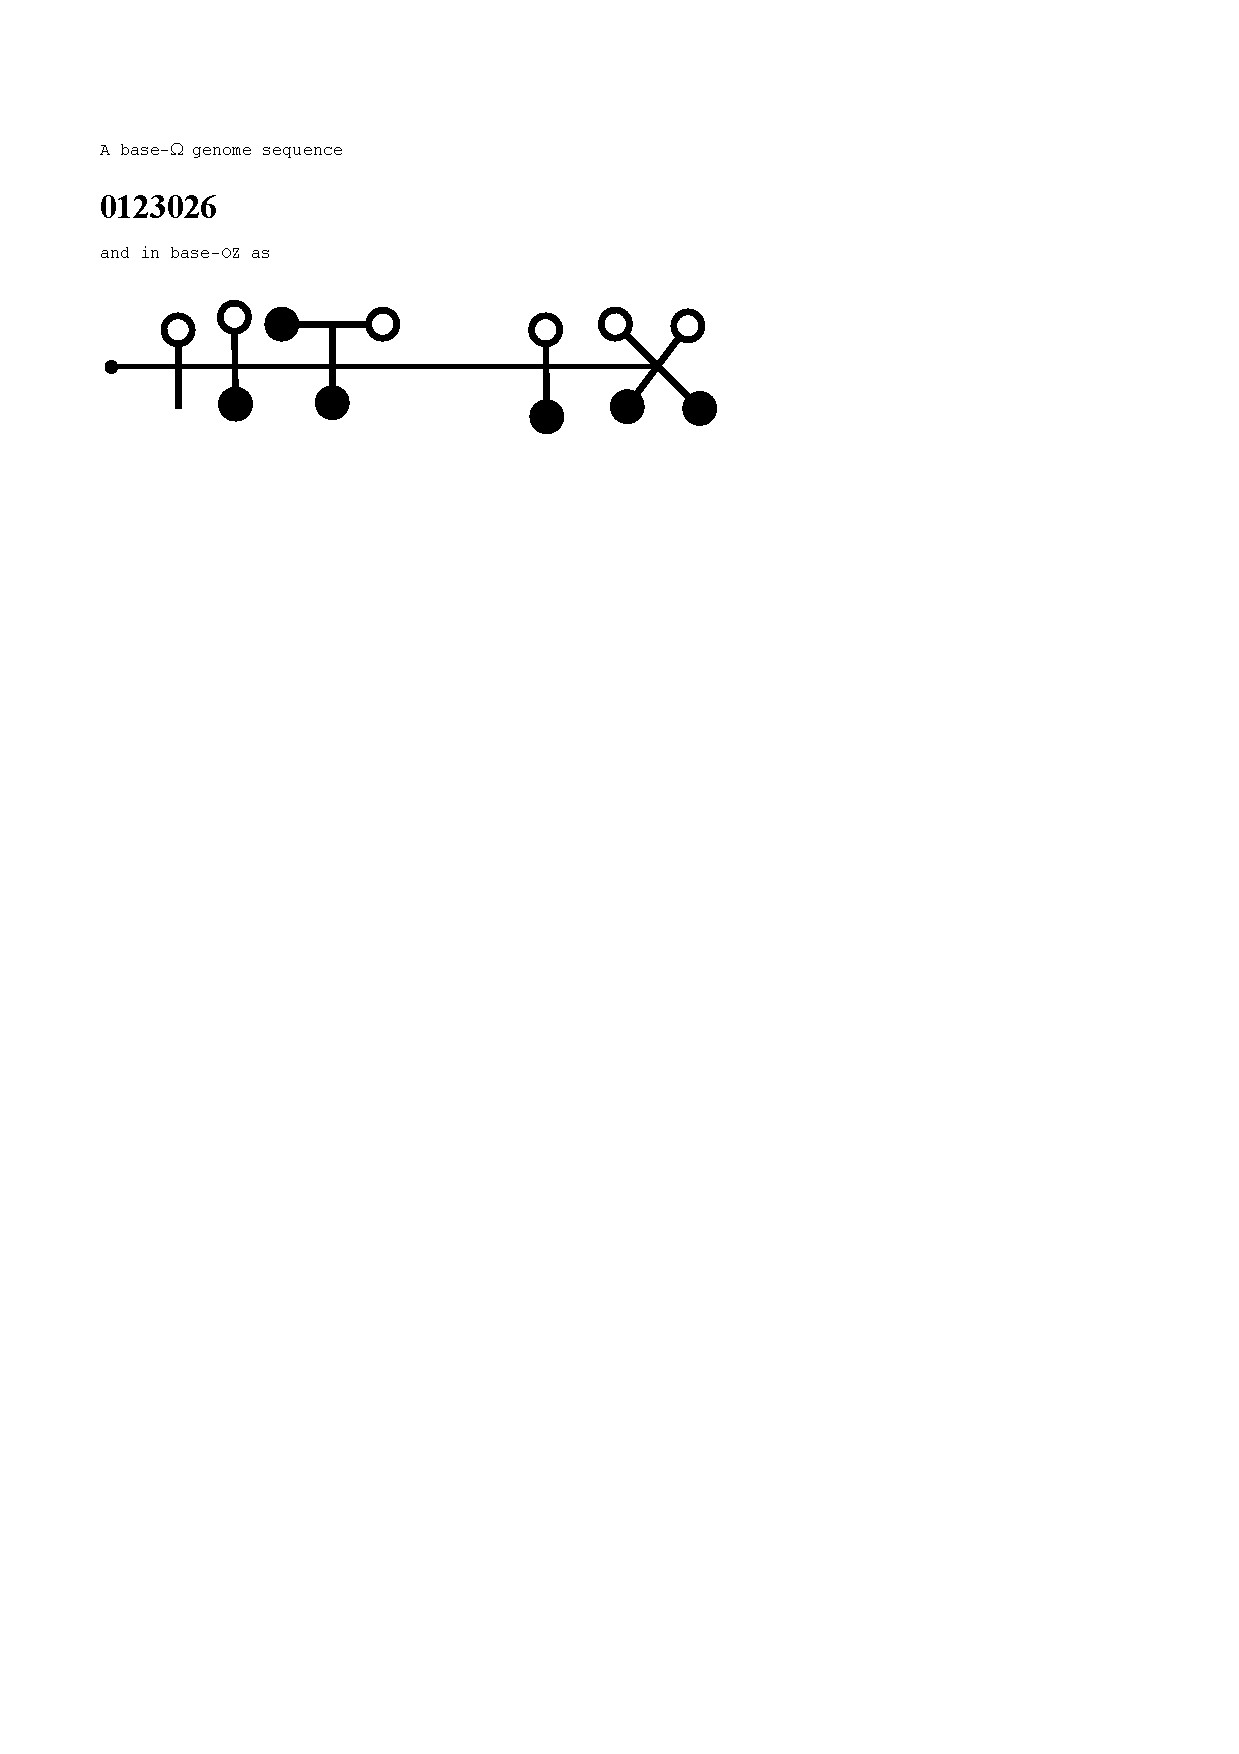
\includegraphics[trim=0cm 20cm 0cm 0cm, clip, width=0.9\textwidth,]{resources/pdfs/OZINCIPHER-APP3-EXA.pdf}\\
   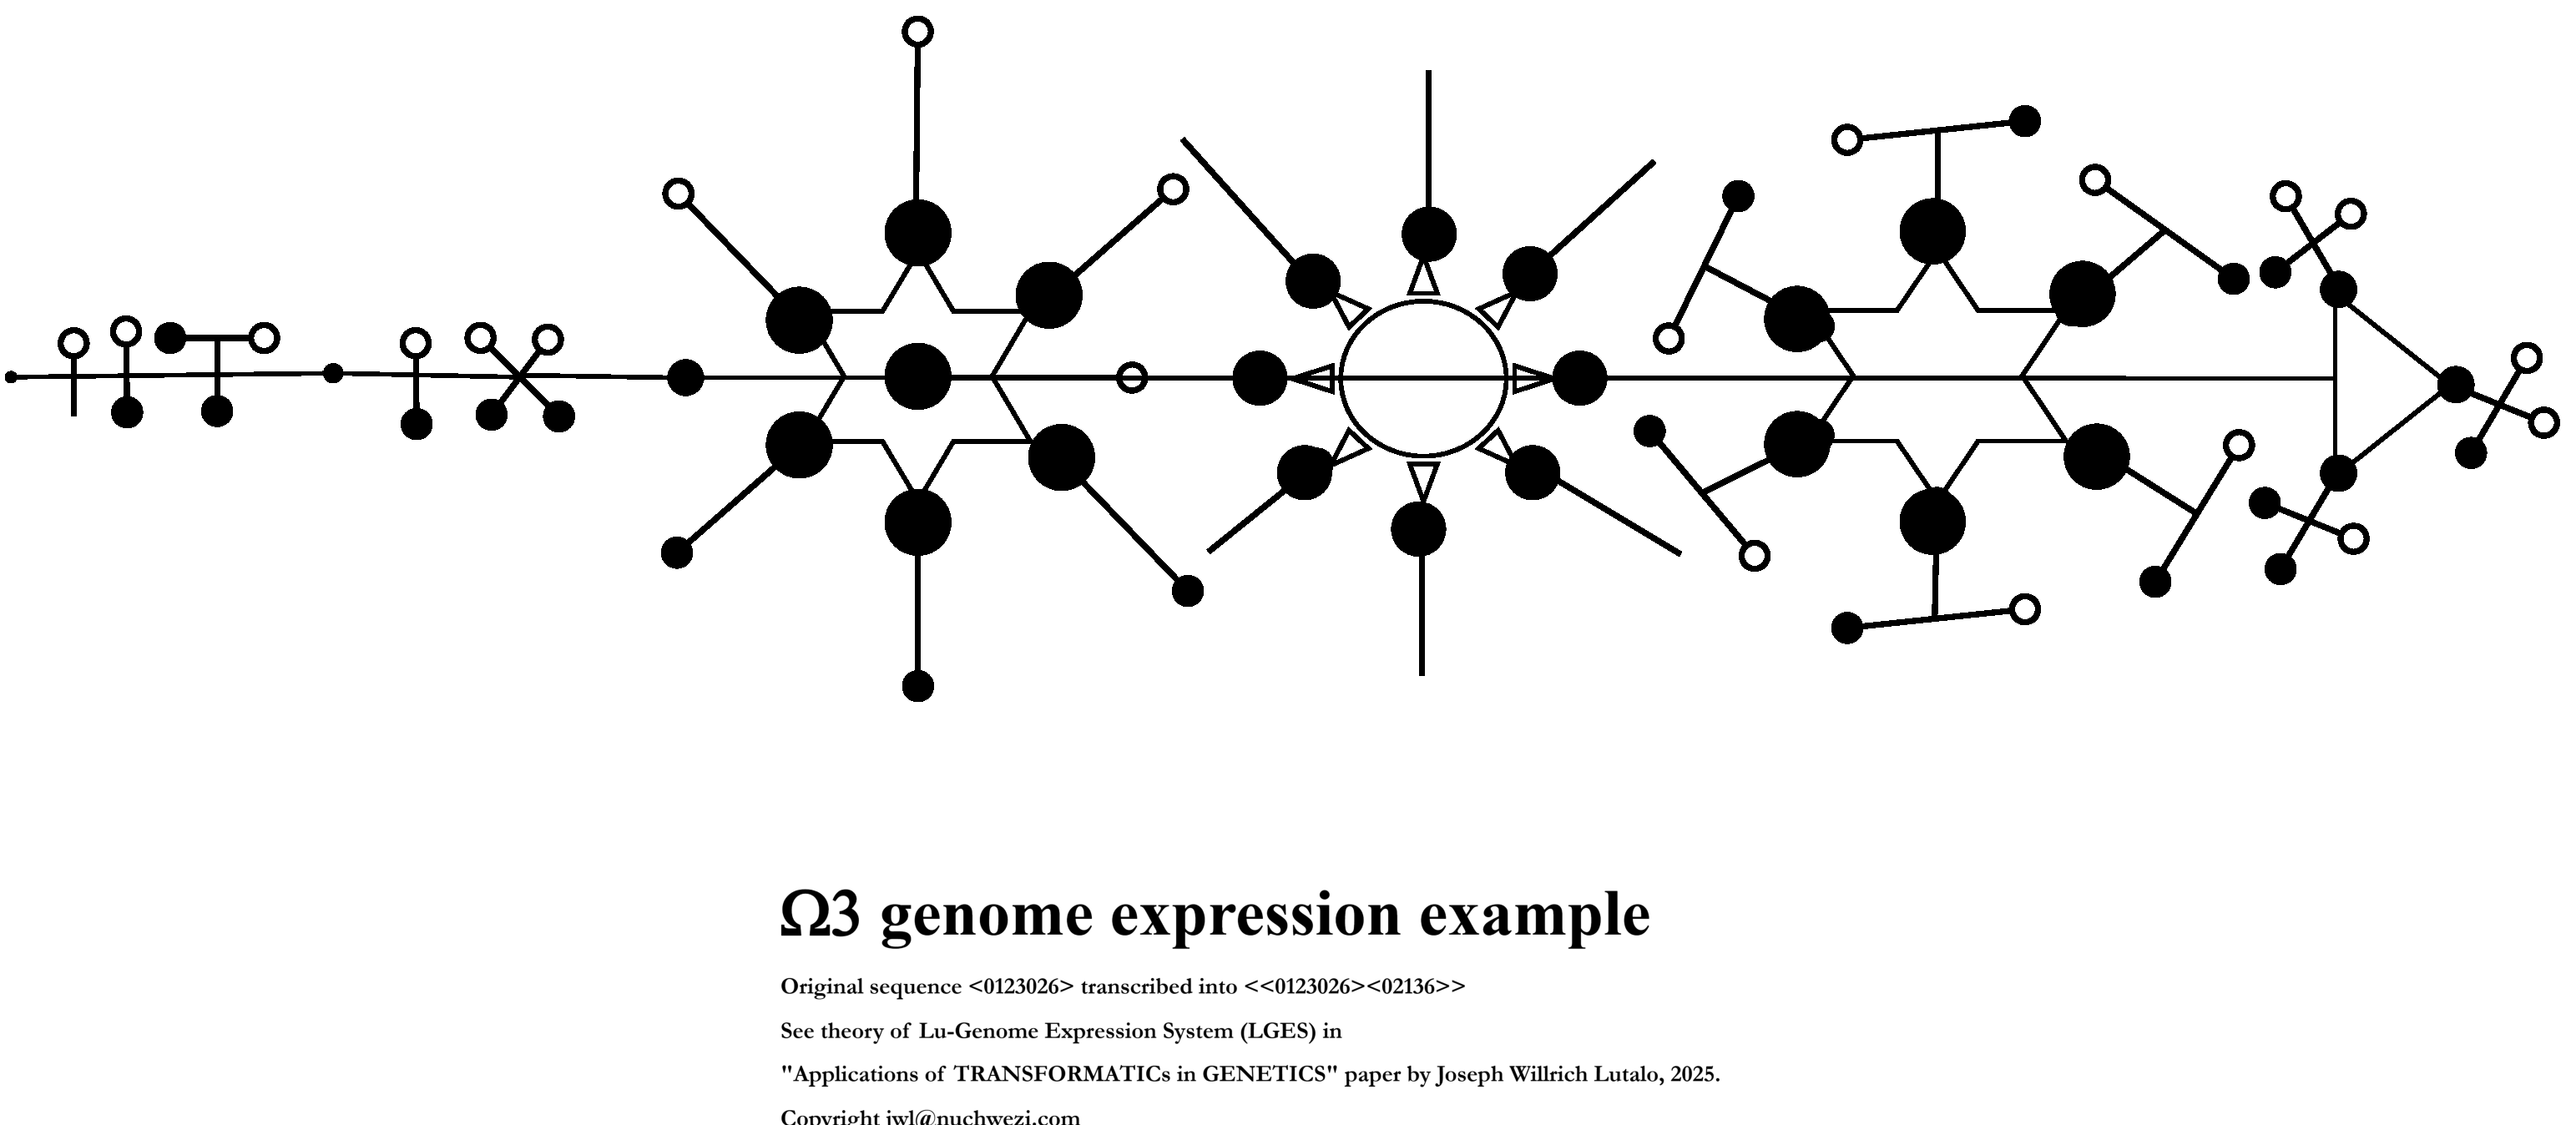
\includegraphics[trim=0cm 0cm 0cm 0cm, clip, width=0.9\textwidth,]{resources/pdfs/PLATONIC-EXA-landscape_ORIG.pdf}\\
      \caption{The equivalent LGES complete genome expression of the $\Omega_{3}$ genome sequence (from \textbf{\hyperref[EQDNEXA]{Equation \ref{EQDNEXA}}})}
  \label{FIGPLATONICEXA_ORIG}
  \end{center}
\end{figure}


Though we won't delve into exploring all kinds of possible \textit{interesting} scenarios with regards to the \textbf{LGES}, we can look at one other example and then move on. From the example hypothetical genome sequences we have encountered, perhaps let us revisit \textbf{\hyperref[EQDNAV]{Equation \ref{EQDNAV}}} and see what the \textbf{Euler Virus} might look like when fully expressed in this system.

So, note that, we already did the first-leg of \textbf{\hyperref[ALGCOZINPLATO_ORIG]{Algorithm \ref{ALGCOZINPLATO_ORIG}}}, and have seen what the \textbf{FGE} prefix --- the \textbf{IFA}, would look like in \textbf{\hyperref[FIGOZEVIRUS]{Figure \ref{FIGOZEVIRUS}}}. So, like we did for $\Omega_{3}$ in the last exploration, let us start by looking at what the numeral-equivalence of the processed $\Omega_{veuler}$ would be like. For brevity, we can sum up the entire production/transformation that leads to the complete \textbf{FGE} with correct prefix and suffix, and thus $\boxed{OZ(\Omega_{veuler})}^*$ as:

\begin{center}
\fbox{
\begin{minipage}{\textwidth}

\begin{trans}
\label{TRANSGENSEQEVIRUS_ORIG}
$\Omega_{veuler} = \langle 2,7,1,8,2,8,1,8 \rangle \rightarrow \hbar(\overset{>}{\Omega_{veuler}}) = \text{\textbf{8}3\textbf{2}2\textbf{1}2\textbf{7}1} \rightarrow \overset{>}{\Omega_{veuler}} = \langle 8, 2, 1, 7 \rangle \implies \boxed{OZ(\Omega_{veuler})} \approx \lnot{\langle 8, 2, 1, 7  \rangle_{pf}} \implies \boxed{OZ(\Omega_{veuler})}^* =  \langle 2,7,1,8,2,8,1,8 \rangle_{oz}\cdot\boxed{\langle 1, 7, 8, 2 \rangle}_{pf}$\\
\end{trans}

\end{minipage}}
\\
\end{center}


Note that, in the derivation depicted in \textbf{\hyperref[TRANSGENSEQEVIRUS_ORIG]{Transformation \ref{TRANSGENSEQEVIRUS_ORIG}}}, one of the most tricky parts is computing that \textbf{FGE} suffix, $\boxed{OZ(\Omega_{veuler})}$, the \textbf{PFA} --- which is formalized/defined by \textit{especially}\footnote{\textbf{\hyperref[EQEXTFGEJOINTSUF_ORIG]{Equation \ref{EQEXTFGEJOINTSUF_ORIG}}} is what covers the special symbol `0', that is treated as a JOINT/GAP in the \textbf{PFA} and as STOP/GAP in \textbf{IFA}.} \textbf{\hyperref[EQFBOXED_ORIG]{Equation \ref{EQFBOXED_ORIG}}}. So, once that is done, then we have our final numeral-\textbf{FGE} expressible as such:\\

\begin{equation}
\label{EQGFEEVIRUS_ORIG}
\boxed{OZ(\Omega_{veuler})}^* =  \langle 2,7,1,8,2,8,1,8 \rangle_{oz}\cdot\boxed{\langle 1, 7, 8, 2 \rangle}_{pf}
\end{equation}\\

Of course, concerning \textbf{\hyperref[EQGFEEVIRUS_ORIG]{Equation \ref{EQGFEEVIRUS_ORIG}}}, note that, or rather, keep in mind that concerning the \textbf{PFA} component, $\boxed{OZ(\Omega_{veuler})}$, the corresponding associated sequence in numeral form is the \textbf{IFA MSS}, $\overset{>}{OZ(\Omega_{veuler})} = \overset{>}{\Omega_{veuler}} = \langle 8, 2, 1, 7 \rangle$. And thus, using necessary transcription and translation ciphers as well as the multiplication rules required by \textbf{\hyperref[EQFBOXED_ORIG]{Equation \ref{EQFBOXED_ORIG}}} when treating of the \textbf{PFA}, we then generate the final genome expression for the \textbf{Euler Virus} under the \textbf{LGES} that looks as in \textbf{\hyperref[FIGLGESEULERVIRUS_ORIG]{Figure \ref{FIGLGESEULERVIRUS_ORIG}}}.


\begin{figure}[H]
  \begin{center}
  %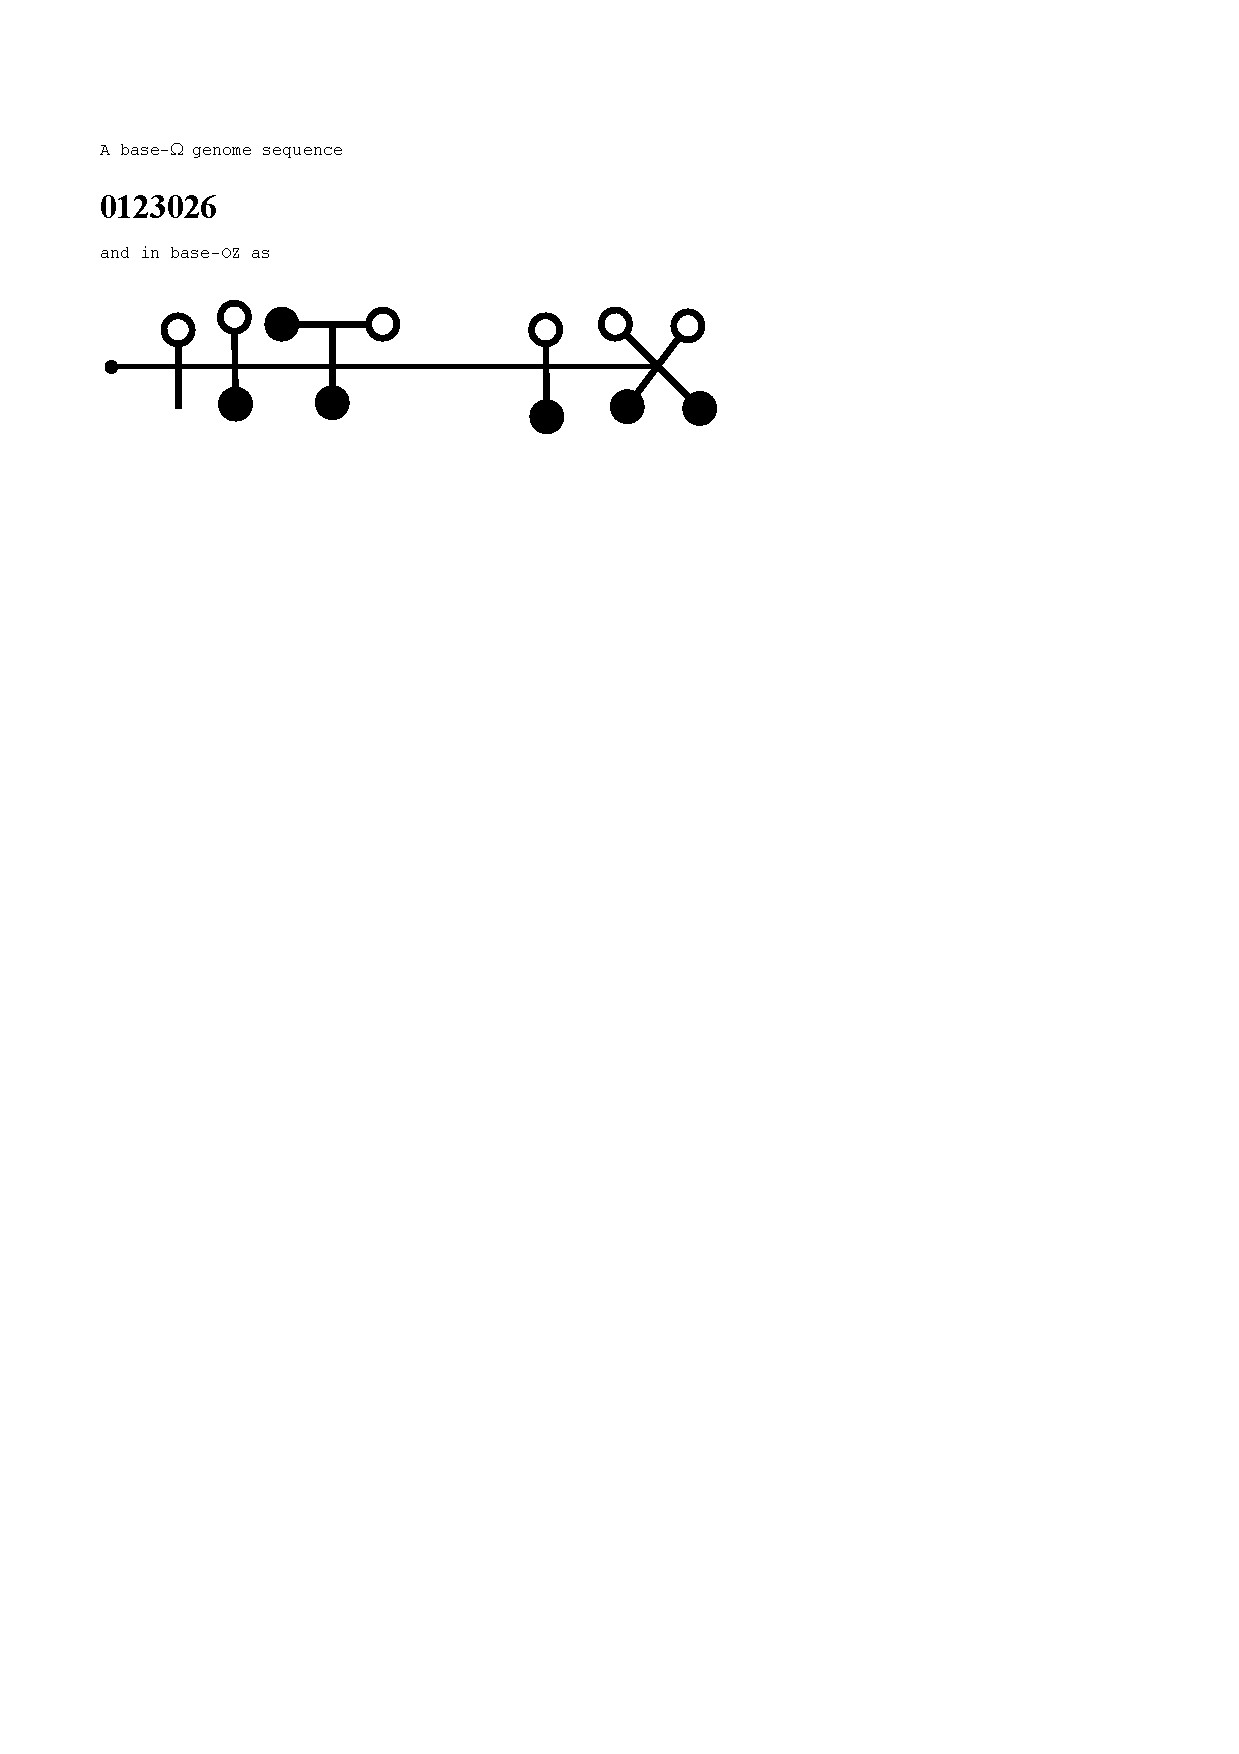
\includegraphics[trim=0cm 20cm 0cm 0cm, clip, width=0.9\textwidth,]{resources/pdfs/OZINCIPHER-APP3-EXA.pdf}\\
   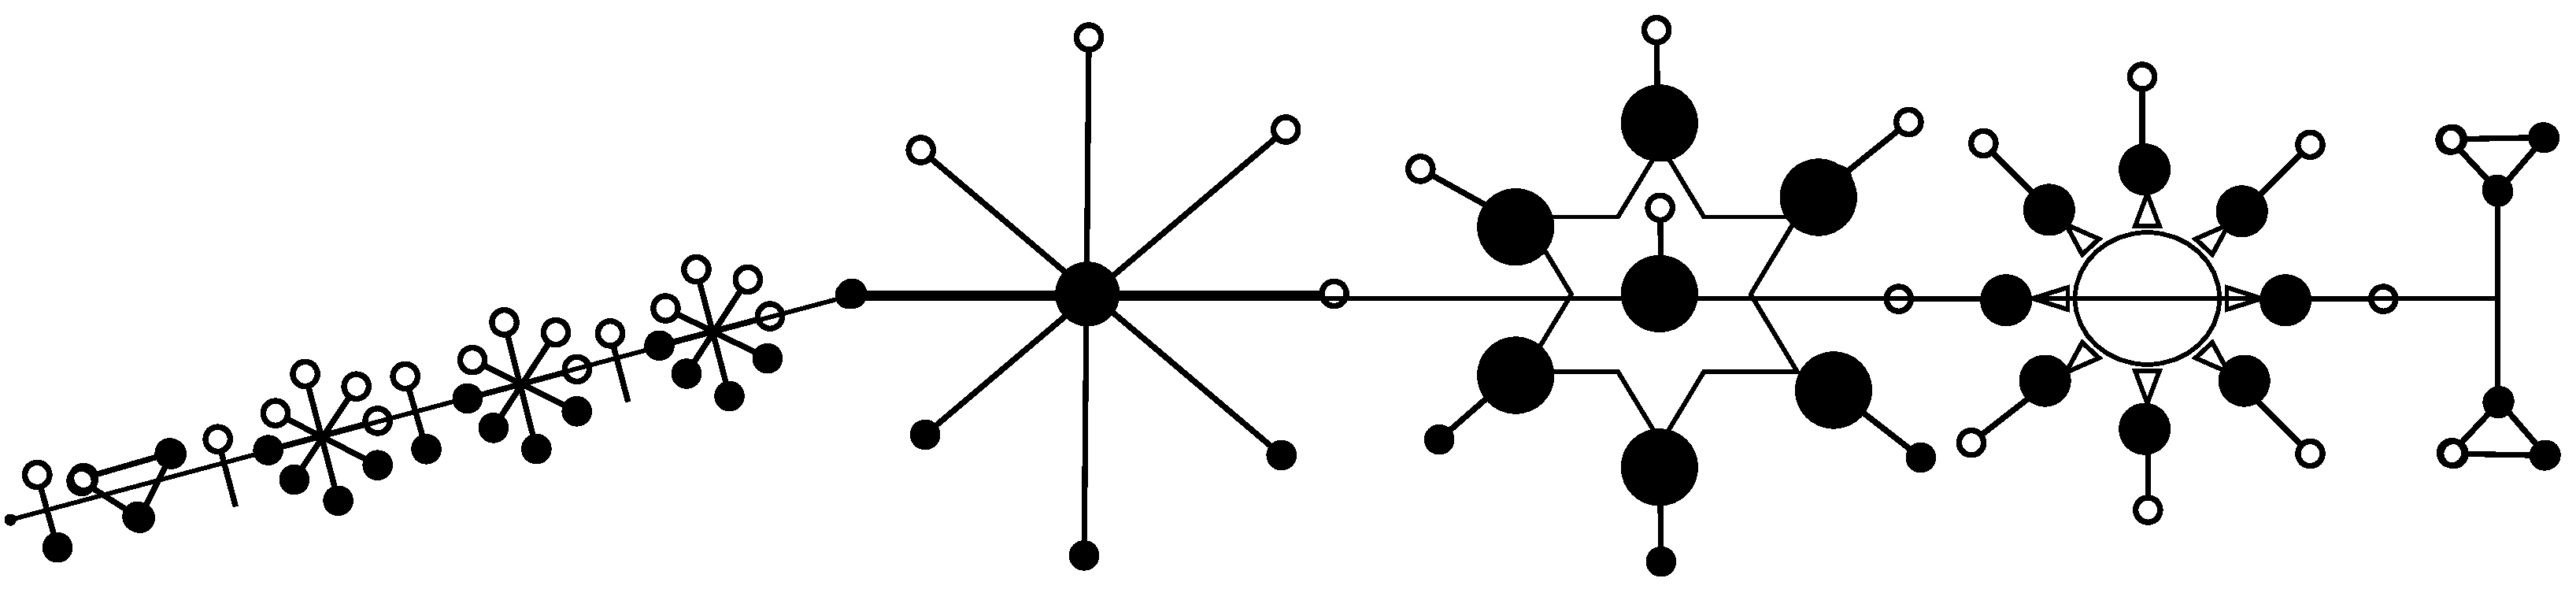
\includegraphics[trim=0cm 0cm 0cm 0cm, clip, width=0.9\textwidth,]{resources/pdfs/PLATONIC-EULERVIRUS-landscape_ORIG.pdf}\\
      \caption{The equivalent LGES complete genome expression of the $\Omega_{veuler}$ (Euler Virus) genome sequence (from \textbf{\hyperref[EQGFEEVIRUS_ORIG]{Equation \ref{EQGFEEVIRUS_ORIG}}})}
  \label{FIGLGESEULERVIRUS_ORIG}
  \end{center}
\end{figure}


Now, concerning that rendering of the genome sequence expressed in \textbf{\hyperref[EQGFEEVIRUS_ORIG]{Equation \ref{EQGFEEVIRUS_ORIG}}}, it might be worth noting, that unlike the earlier examples of \textbf{LGES} expressions, we have taken the liberty to exploit that special joint that kick-starts the \textbf{PFA}, or rather, which separates the \textbf{IFA} from the \textbf{PFA} in a \textbf{FGE} expression. So, just like an organism with a physical joint might sometimes appear as angled or curved, so we have chosen to depict the $\Omega_{veuler}$ with its one joint\footnote{Definitely, and interesting to explore, a genome sequence with multiple JOINT points in it might be how an organism with say, multiple appendages, such as legs, hands, and a head that can move independently of the core/thorax of the body is possibly arrived at. The interested student should go ahead and explore more non-trivial $\Omega$-base sequences just to see what's possible.} well utilized. However, and important to note; it is not just joints that might appear different across different renderings of the same basis genome sequence. So, in \textbf{\hyperref[FIGLGESEULERVIRUSv2_ORIG]{Figure \ref{FIGLGESEULERVIRUSv2_ORIG}}}, we see another variation of the same sequence, with readily noticeable differences being the IFA-PFA joint in its neutral position, and then the second node in the PFA (corresponding to \textbf{$7_{pf} \otimes 2_{oz}$} or rather \textbf{$7_{pf} + 7 \times 2_{oz}$}) with the $2_{oz}$ appendages depicted mostly aligned horizontally --- more accurately, \textit{tangentially}, while in the former expression, they were all perpendicular/orthogonal to the platonic form they are appended to.


\begin{figure}[H]
  \begin{center}
  %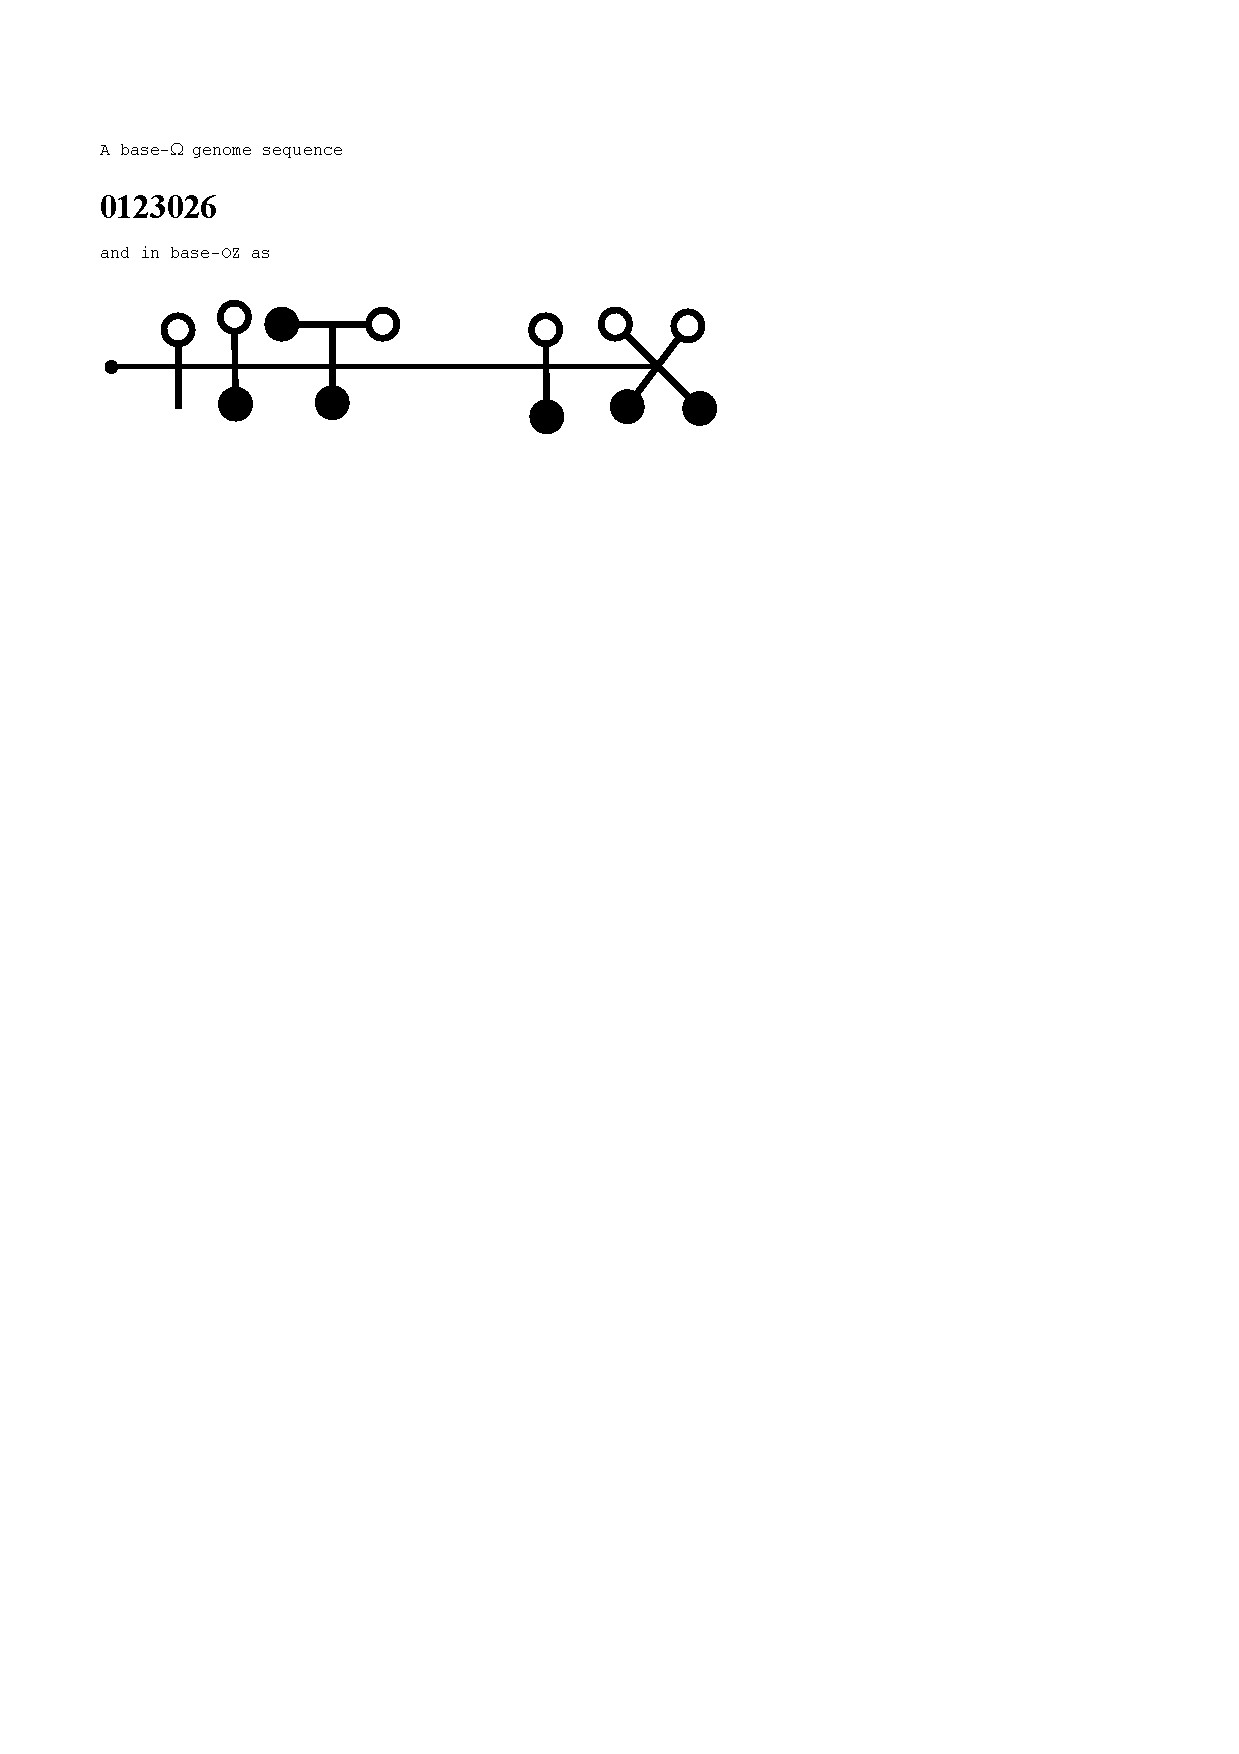
\includegraphics[trim=0cm 20cm 0cm 0cm, clip, width=0.9\textwidth,]{resources/pdfs/OZINCIPHER-APP3-EXA.pdf}\\
   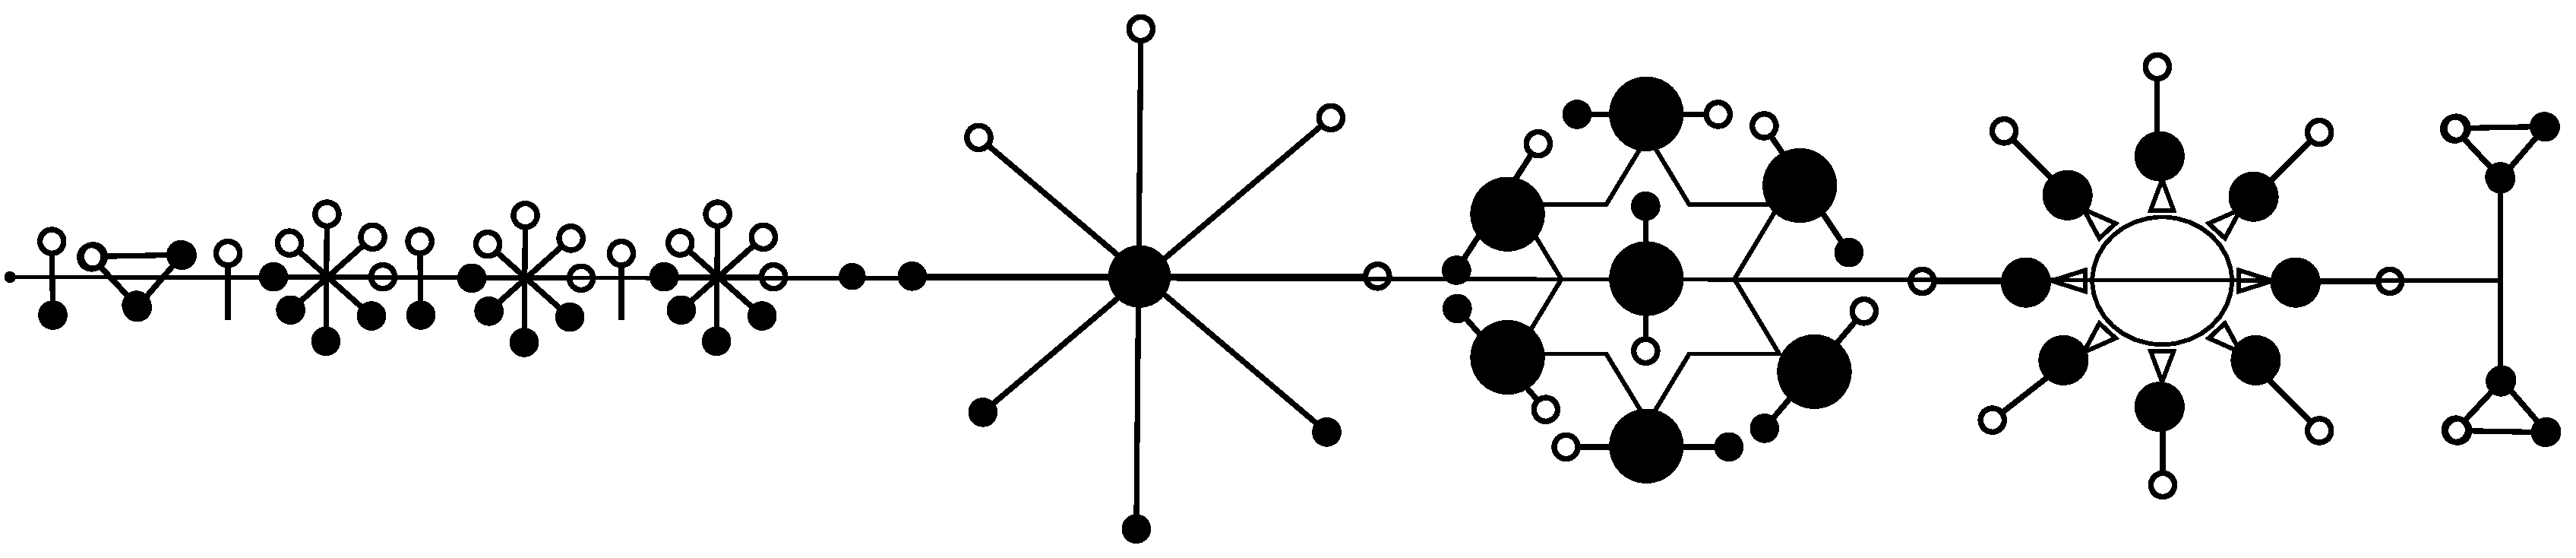
\includegraphics[trim=0cm 0cm 0cm 0cm, clip, width=0.9\textwidth,]{resources/pdfs/v2-PLATONIC-EULERVIRUS-landscape_ORIG.pdf}\\
   \caption{The \textbf{alternative rendering}  of the same sequence as $\Omega_{veuler}$.}
  \label{FIGLGESEULERVIRUSv2_ORIG}
  \end{center}
\end{figure}

Concerning \textbf{\hyperref[FIGLGESEULERVIRUSv2_ORIG]{Figure \ref{FIGLGESEULERVIRUSv2_ORIG}}}, the alternative rendering  of the same sequence as $\Omega_{veuler}$ first depicted in \textbf{\hyperref[FIGLGESEULERVIRUS_ORIG]{Figure \ref{FIGLGESEULERVIRUS_ORIG}}}, we see that underlying the variations is how the \textit{degrees of freedom} in rendering the genome have somewhat been exploited. Notice how the joint and appendages are placed or oriented about the platonic forms that mostly remain unchanged across the two renderings --- except perhaps in scale. And talking of scaling nodes, in the future, we might want to explore whether in such a system as \textbf{LGES} in which the expression is sensitive to measures such as the \textbf{IFA MSS}, whether it might make sense to scale each subsequent pf-node in the \textbf{PFA} based on its position within the sequence? Though we didn't have such a rule included in \textbf{\hyperref[ALGCOZINPLATO_ORIG]{Algorithm \ref{ALGCOZINPLATO_ORIG}}}, and yet, our example renderings here have somewhat taken advantage of that plausible logic.

That said, note that, we started this work with a photograph of a pineapple ready to harvest (see \textbf{\hyperref[FIGPINEAPPLE]{Figure \ref{FIGPINEAPPLE}}}), and though the associated discussion\footnote{Checkout video/mini-lecture on the matter at author's YouTube: \url{https://youtube.com/shorts/yTJzBEpw7Z4}} by the author did bring up the matter of how it might inspire a genome expression system in which the prefix is the actual DNA that renders the rest of the organism (fruit, plant-base and roots in this case of the pineapple), it is left as an exercise to the reader, to decide whether example genome sequence expressions/renderings such as in \textbf{\hyperref[FIGLGESEULERVIRUS_ORIG]{Figure \ref{FIGLGESEULERVIRUS_ORIG}}} depict this pineapple-inspired philosophy or not.


%%%%%%%%%%%%%%%| TRANSFORMATICS 101 - explained mini-booklet as an appendix chapter |%%%%%%%%%


% insert [front] cover --- could just be a PNG or PDF
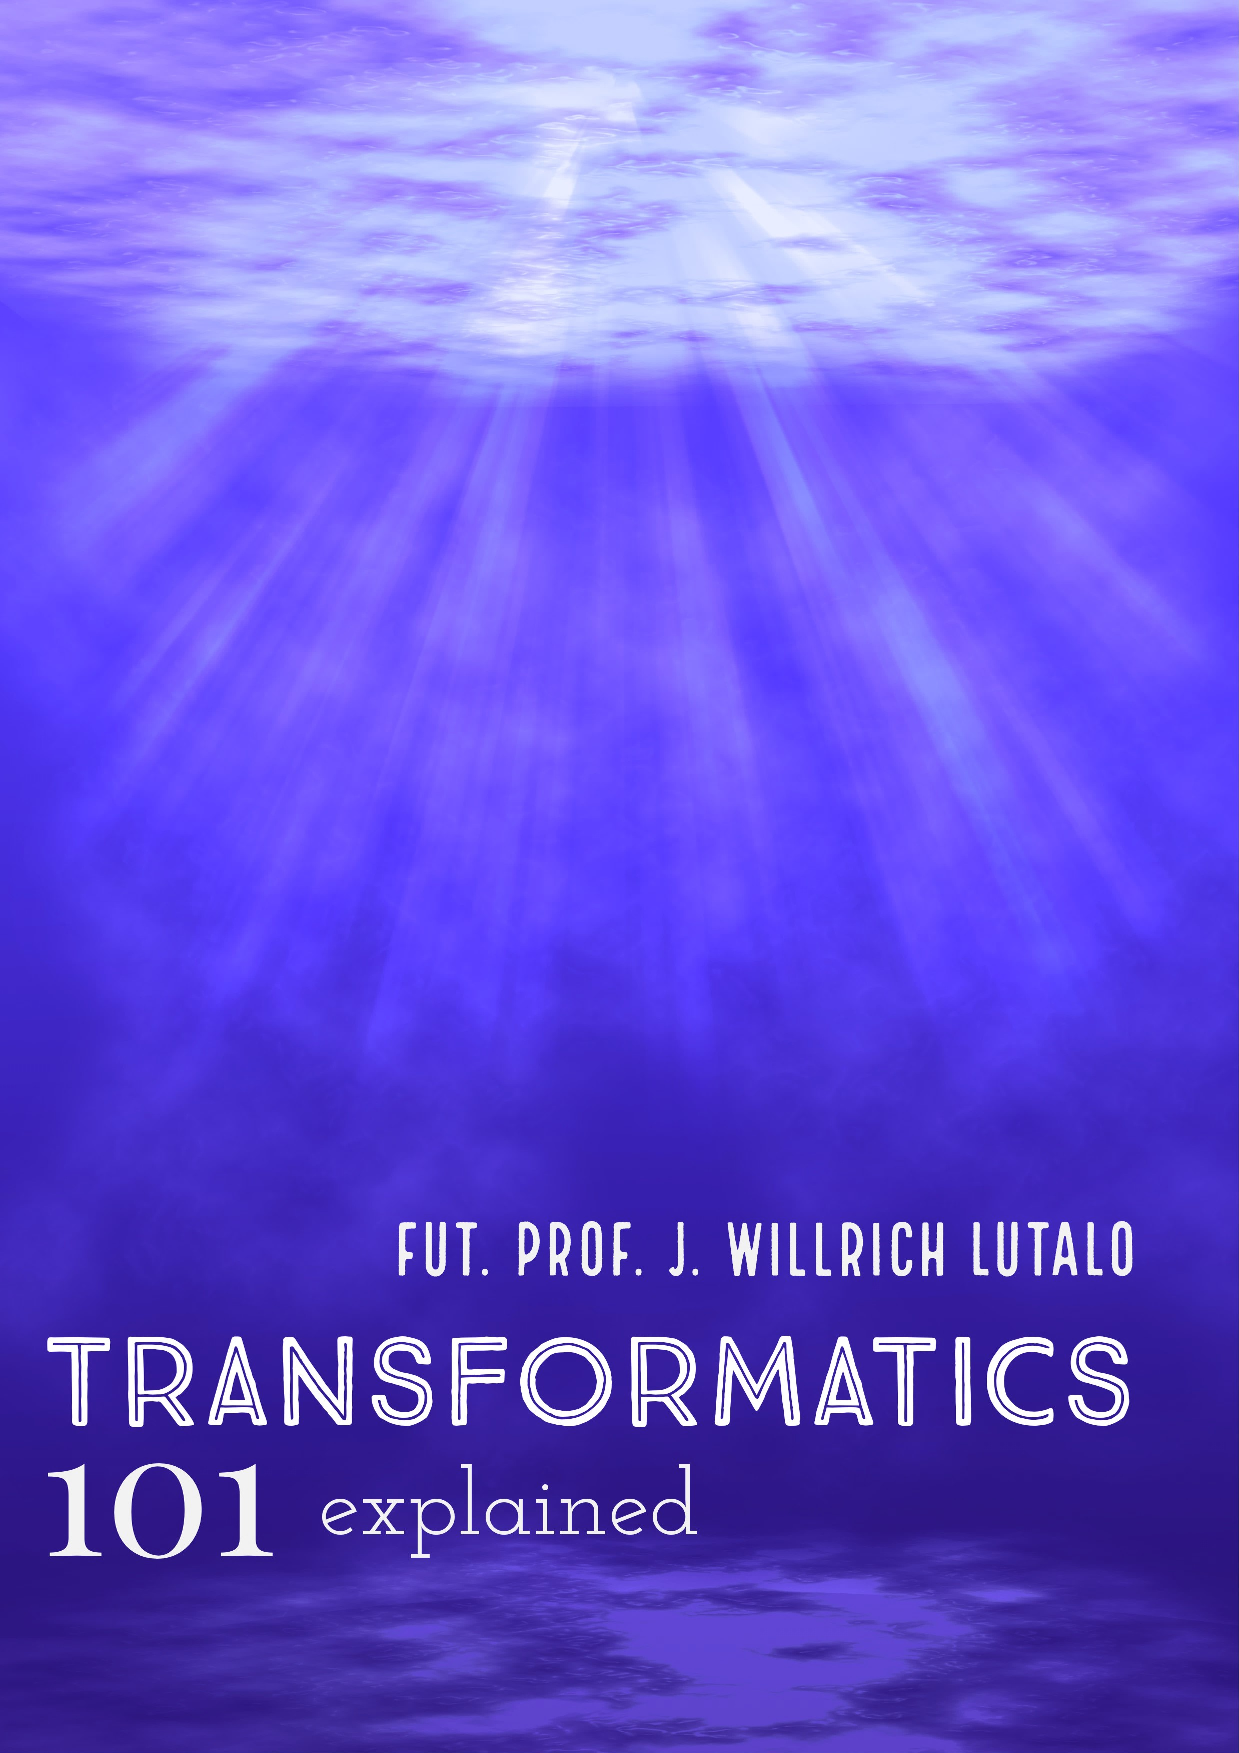
\includepdf[pages=1]{resources/pdfs/trans_front_cover.pdf}

\chapter{TRANSFORMATICS 101 - explained:\\\small{A rigorous, succinct introduction to all the essential foundations and proposed theory of Transformatics}}
\label{CHAPTRANS}

\section*{ABSTRACT\footnote{Note that this chapter attempts to present \cite{Lutalo2025_transformatics_thesis} verbatim, with the only major difference being the numbering of citations and references, which are co-shared with the main manuscript.}:}
%\Large
In only \textbf{10 general foundational results}\cite{lutalo_2025_trans101_1page} --- all \textbf{based on earlier mathematical research} by the author, as well as \textbf{10 extra abstractions} spanning \textbf{how transformatics might be leveraged} as \textbf{a basis mathematics} \texttt{for problems} in; \texttt{number theory} and \texttt{cryptography} (o-SSIs); \texttt{mathematical statistics} (ADM, TCR, PCR, MSS, SC, PC); \texttt{linear algebra} (super sequences); \texttt{computer science} (TEA language, transformer-chains or sequence-transformers) and \texttt{information theory} (entropy of a sequence) among others, we distill and establish, in a summarized form, the \textbf{core foundations of Transformatics}\cite{transformatics} as its own mathematical theory, branch, or \textbf{discipline}. In this \textbf{mini-thesis}. Each foundational result presented is likewise accompanied by one or \textbf{more references} to some earlier work where the idea or presented concept was first developed, presented, or applied by the author during their research. \textbf{Useful notes and commentary} are also included where necessary, and in the extension decade of \textbf{proposed abstractions}, also commentary about how the proposals relate to the decade of foundational results likewise is catered for.
 \newline\newline
     \textbf{Keywords}: Foundations, Transformatics, Sequence Analysis,  Sequence Transformers, Thesis
%\end{abstract}

\section{Foundations of a New Mathematics of Sequences}
\label{SECFOUND}

\subsection{Result 1: The Empty Sequence\cite{lnspaper}}
\label{RES1}

$\Theta = \langle \rangle \implies |\Theta| = 0 \quad \land \quad \Theta \equiv \emptyset$

\subsection{Result 2: A Symbol Set\cite{Lutalo2024gtnc}}

$\psi_\beta^n = \langle \beta_{i \in [1,n]} \rangle : n \in \mathbb{N} : \invpi(\beta_i \in \psi_\beta) = 1 \quad \forall \beta_i \in \psi_\beta$

\subsection{Result 3: A Sequence\cite{lnspaper}}
\label{RES3}

$\Theta^n = \langle \theta_{i \in [1,n]} \rangle : \mathbb{N} \times \psi_\beta : n \geq 1$

\subsection{Result 4: Sequence Cardinality\cite{adtpaper}\cite{Lutalo2024gtnc}}
\label{RES4}

$\forall \Theta^n = \langle \theta_{i \in [1,n]} \rangle : \mathbb{N} \times \psi_\beta \quad \implies \quad \invpi(\Theta^n) = |\Theta^n| = n \in \mathbb{N}$ 



\subsection{Result 5: A Sequence Symbol Set\cite{ossipaper}\cite{Lutalo2024gtnc}}
\label{RES5}

$\psi(\Theta^n) = \langle \theta_{i \in [1,k]} \rangle : k,n \in \mathbb{N} \land k \geq 1 : \invpi(\theta_i \in \psi(\Theta^n)) = 1 \quad \forall \theta_i \in \Theta^n : k \leq n : \invpi(\psi(\Theta^n)) = k$


\subsection{Result 6: A Sequence Transformation\cite{transformatics}\cite{lnspaper}}

$\Theta^n = \langle \theta_{i \in [1,n]} \rangle : \mathbb{N} \times \psi_\beta \rightarrow \Theta^* = \langle \theta^*_{i \in [1,k]} \rangle : \mathbb{N} \times \psi_* : \psi_\beta \neq \psi_{*} \lor \psi(\Theta^n) \neq \psi(\Theta^*) \lor \overset{>}{\psi}(\Theta^n) \neq \overset{>}{\psi}(\Theta^*)$


\subsection{Result 7: A Sequence Transformer\cite{Lutalo2025transpsy}\cite{transformatics}}
\label{RES7}

$\Theta^n = \langle \theta_{i \in [1,n]} \rangle : \mathbb{N} \times \psi_\beta \xrightarrow{f(\Theta)=\Theta^*} \Theta^* = \langle \theta^*_{i \in [1,k]} \rangle: \mathbb{N} \times \psi_* 
; \quad \psi_\beta \neq \psi_{*} \lor \psi(\Theta^n) \neq \psi(\Theta^*) \lor \overset{>}{\psi_\beta} \neq \overset{>}{\psi_*}$

\subsection{Result 8: A Sequence Filter\cite{transformatics}}
\label{RES8}

$\Theta^n = \langle \theta_{i \in [1,n]} \rangle : \mathbb{N} \times \psi_\beta \xrightarrow{f(\Theta,\psi_{\beta^*})=\Theta^*} \Theta^* = \langle \theta^*_{i \in [1,k]} \rangle : \mathbb{N} \times \psi_{\beta^*} ;\\ k \in \mathbb{N} : \psi_{\beta^*} \subseteq \psi_\beta \implies \invpi(\psi_{\beta^*}) = k \leq \invpi(\psi_\beta) \implies \invpi(\Theta^*) \leq \invpi(\Theta^n) $

\subsection{Result 9: A Sequence Generator\cite{transformatics}\cite{lutalo2025transformatic}}
\label{RES9}

$\Theta^n | \emptyset \xrightarrow{f(\psi_\beta,k))=\Theta^*} \Theta^k = \langle \beta^*_{i \in [1,k]} \rangle : \mathbb{N} \times \psi_{\beta} : k \in \mathbb{N} : \forall \beta_i \in \Theta^k \implies  k \geq 1 \quad \land \quad \beta_i \in \psi_\beta = \Psi^\infty \cup \Theta^n$

\subsection{Result 10: A Sequence Sampler\cite{lutalo_2025_trans_genetics}}

$\Theta^n \xrightarrow{f(\Theta^n,k))=\Theta^k} \Theta^k = \langle \theta_{i \in [1,k]} \rangle : \mathbb{N} \times \psi(\Theta^n) : k,n \in \mathbb{N} \land k \geq 1$


%%%---------[ EXTENSION ]-----------%%%

{
\noindent\rule{\linewidth}{0.4pt}

\textbf{NOTES:}

\begin{enumerate}
\item \textbf{Result 1}: Apart from the concept of the set, that of the \textbf{empty set} underlies all of transformatics --- it is the ideological basis of all kinds of sequence generation, in particular, when projected unto the \textbf{empty sequence}. It allows us to codify states such as emptiness, non-emptiness, equality, identity, \textbf{zero} etc. 
\item \textbf{Result 2}: The \textbf{symbol set} underlies of all formulations in need of a way to speak of or quantify the \textbf{identity composition} of any sequence.
\item \textbf{Result 3}: The \textbf{sequence} is the basis concept in transformatics when applied to sequences, or rather, the \textbf{algebra of sequences}\cite{treealgebras_review}.
\item \textbf{Result 4}: \textbf{Sequence cardinality} allows us to quantify various measures about a sequence relative to the size of its membership at rest. These might for example be measures such as the entropy of the sequence (\textbf{\hyperref[PROPTOE]{Proposal 10}}).
\item \textbf{Result 5}: The \textbf{sequence symbol set} is an application of the symbol set concept to any particular sequence as opposed to say, talking of the symbol set of a language --- an alphabet like $\psi_{az}$ or $\psi_{0-9}$ for example Also, when applied to a particular sequence, such a ordered set might also reflect the order of members in the concerned sequence --- somewhat similar to the MSS (\textbf{\hyperref[PROP5]{Proposal 5}}) then, but not the same.
\item \textbf{Result 6}: Underlying all notions of one sequence being \textit{different} from any other sequence is that of \textbf{sequence transformations}. Any operation that can alter either the composition or member-ordering of a sequence is essentially a sequence transformer. And when we talk of any two or more sequences in terms of how they differ from each other irrespective of the process or operation that maps them between each other, we then speak of a \textbf{sequence transformation}. In the latest (1$^{st}$ November 2025) update to these foundations, we have also introduced use of the concept of the \textbf{modal sequence statistic} in some of the specifications such as for the definition of sequence transformation as a concept. This, especially so we can enhance or make more robust, the foundational result. Otherwise, we formally [re-]introduce the concept of the MSS in \textbf{\hyperref[PROP5]{Proposal 5}}.
\item \textbf{Result 7}: The \textbf{sequence transformer} concept concretizes the notion of a transformer operation underlying or betwixt any two sequences involved in a sequence transformation. Such transformers might be operations such as those specified on structures such as matrices in linear algebra, or might be as the structure-preserving sequence altering functions as the catamorphisms that Gibbons mentions in relation to transformations on trees\cite{treealgebras_review}. Also realize that in the current formulation of \textbf{Result 7}, we employ the concept of the MSS in specifying the final potential kind of sequence transformation possible --- where the composition and cardinality of a sequence pre and post transform might stay preserved, but not the relative order of terms within the sequence --- a concept also precisely analyzable using mathematics and measures such as the \textbf{anagram distance measure} (\textbf{\hyperref[PROP2]{Proposal 2}}).
\item \textbf{Result 8}: \textbf{Sequence filters} allow us to specify or treat of scenarios in which one sequence is reduced to a smaller, perhaps more useful sequence --- such as the generation of an MSS or any symbol set for that matter, from any arbitrary sequence. Note that since the 8$^{th}$ October first edition of these foundations, \textbf{Result 8} has since been fixed/corrected, so that the current transformer specification for a generic sequence filter is the correct one --- also more specific than originally.
\item \textbf{Result 9}: Underlying any concept of \textit{creation} is that of bringing things to life.. (\textit{ex nihilo or not}) especially relative to some pattern or specification (such as the generation of words in some specified language or number system or alphabet, etc.), but also, generation of structures or objects of a particular kind or type. Concerning the current general specification of a [sequence] generator, note that first of all, any sequence generator is essentially a sequence transformer to begin with. Moreover, for the fact that the generated sequence might sometimes span an alphabet, type or symbol-set different or larger than that of the source or original reference sequence --- such as a seed-symbol-set $\psi_\beta$ in the presented general case --- we also could have expressed the final specification as either $\beta_i \in \psi(\Theta^n) \cup \psi^\infty$ or perhaps $\psi_\beta := \psi_\beta | \psi_\beta \cup \psi(\Theta^n) \cup \psi^\infty | \psi^\infty$ and where we know that $\psi(\Theta^n) \subseteq \Theta^n$.
\item \textbf{Result 10}: Being able to \textbf{choose} is a fundamental concept in mathematics such as probability theory but also much of statistical experiments\cite{lutalo2025rng} or intelligent behavior\cite{Lutalo2025transpsy} for example. We might liken a \textbf{sequence sampler} to a sequence filter (\textbf{Result 8}), but they are not the same thing; they approach the same concept differently; a filter  might be the source sequence minus everything not matching a pattern, while the sampler could be modeled as the source sequence minus everything matching a pattern or vice-versa.

\end{enumerate} 

}
\noindent\rule{\linewidth}{0.4pt}


\section{Proposed Abstractions Leveraging Transformatics}
\label{SECPROP}

Before we kick-off, note that, as in many previous works on transformatics since \cite{transformatics}, when we have any sequence $\Theta^n : \forall i \in [1,n] : \exists \theta_i \in \Theta^n$, then, when we wish to talk of the \textbf{position index} of some member element or symbol $\theta_i$ in $\Theta^n$, such that we mean the member in that sequence that is located or positioned at exactly index $i$ in the range $[1,n]$, then we shall, as introduced and elaborated upon in the introduction section of \cite{transformatics}, merely use the notation:

\vspace{1em}
\begin{equation}
I(\theta_i, \Theta^n) = i \quad \forall \theta_i \in \Theta^n
\end{equation}
\vspace{1em}

Further, if we have any two elements from the sequence (whether or not they are equal: $\theta_i = \theta_j$ or not: $\theta_i \neq \theta_j$), and yet, if $i \neq j$, then $I(\theta_i, \Theta^n) \neq I(\theta_j, \Theta^n)$, and if $i \leq j$, then $I(\theta_i, \Theta^n) \leq I(\theta_j, \Theta^n)$. 

As you shall come to appreciate when studying formulations and expressions in transformatics, the position operator or measure, $I(\cdot, \cdot)$ is very fundamental, useful and indispensable especially when treating of (sic) \textbf{ordered sequences} or of order in any sequence.

\subsection{Proposal 1: The o-SSI Sequence from any Sequence\cite{ossipaper}}

Assume we consider the sequence $\Theta: \mathbb{N} \times \psi_*$ of any length and spanning an arbitrary symbol set $\psi_*$. Then, in case we wish to reduce $\Theta$ to a representative sequence $\Theta_{ossi}$ that only contains elements of $\Theta$ spanning the symbol set, $\psi_\beta$, of some particular base, $\beta$; in which case, $\Theta_{ossi}$ would be an \textbf{orthogonal symbol set identity} (o-SSI) sequence under base-$\beta$, then, the following o-SSI-generator --- also \textbf{an extractor}\footnote{In the sense that, where a sequence already contains the essential symbols spanning some particular symbol set, and even though they might be scattered about or `buried' around in the sequence surrounded by `noise', the function would merely extract those essential symbols [only,] from that sequence in their natural order of first occurrence.} and \textbf{a reducer} transformer, defined using the calculus and semantics of transformatics, would suffice\footnote{Say, and as almost all transformatics might be in practice --- consists of a clear, succinct and complete specification that can readily be translatable into a working or equivalent computer program based on or defined using the chaining of sequence transformers such as in a language as TEA\cite{cli_tttt}.}:

\vspace{1em}
\begin{transf}[The \textbf{o-SSI Extractor}]
\label{TRANSFOSSIb}
$\Theta \langle \theta_{i \in [1,n]} \rangle: \mathbb{N} \times \psi_*  \xrightarrow{O_{filter}(\Theta,\psi_\beta)} \Theta^k \langle \theta_i \rangle : \mathbb{N} \times \psi_\beta = \Theta_{ossi};\\ 0 \leq k \leq \invpi(\psi_\beta) \leq \invpi(\Theta) = n \in \mathbb{N} : \forall \theta_i \in \Theta^k \implies \exists \theta_i \in \psi_\beta \quad\\
\land \quad \forall i,j \in \mathbb{N} \land \theta_i, \theta_j \in \Theta^k: I(\theta_i,\Theta) \leq I(\theta_j,\Theta) \implies I(\theta_i,\Theta^k) \leq I(\theta_j,\Theta^k) $
\end{transf}
\vspace{1em}


First, realize that \textbf{\hyperref[TRANSFOSSIb]{Transformer \ref{TRANSFOSSIb}}} leverages the concept of a sequence filter as first introduced in \textbf{\hyperref[RES8]{Foundational Result 8}}. Also, note that, the \textbf{o-SSI Sequence}, $\Theta_{ossi}$, of any sequence $\Theta$ under $\beta$ would likewise be related to the concept of the \textbf{Specific Symbol Set}\footnote{Refer to \textbf{Definition 3} in \cite{ossipaper}}, $\hat{\psi}_\beta(\Theta)$, of that sequence, in the sense that, at most, $\Theta_{ossi}$ is equivalent to $\hat{\psi}_\beta(\Theta)$  or that their cardinalities and memberships are related as:

\vspace{1em}
\begin{equation}
\invpi(\Theta_{ossi}) \leq  \invpi(\hat{\psi}_\beta(\Theta)) \leq \invpi(\psi_\beta) \leq  \invpi(\Theta)
\end{equation}
\vspace{1em}

and as for membership:

\vspace{1em}
\begin{equation}
\psi(\Theta_{ossi}) \subseteq  \hat{\psi}_\beta(\Theta) \subseteq \psi_\beta \subseteq  \Theta
\end{equation}
\vspace{1em}


\subsection{Proposal 2: The Anagram Distance Between Any Two Sequences\cite{adtpaper}}
\label{PROP2}

Occasionally, one shall find that they need to quantify how different some two or more sequences are. In the simplest case, we might merely sort a collection of sequence by the relative size of each sequence, and thus differentiate them by their sequence cardinality for example --- $\invpi(\Theta)$ Vs $\invpi(\Theta^*)$ for some two sequences involved in a general transformation such as:

\vspace{1em}
\begin{trans}
\label{TRANS1b}
$\Theta \rightarrow \Theta^* \quad \implies \quad \invdel_{\Theta,\Theta^*} = (\invpi(\Theta) - \invpi(\Theta^*));\\
\invdel_{\Theta,\Theta^*} = \begin{cases}
> 0 & \text{compression}\\
 0 & \text{conservation}\\
 < 0 & \text{protraction}
 \end{cases}
$
\end{trans}
\vspace{1em}

or if we only wish to care about absolute distance..

\vspace{1em}
\begin{trans}
\label{TRANS1Ab}
$\Theta \rightarrow \Theta^* \quad \implies \quad |\invdel|_{\Theta,\Theta^*} = |\invpi(\Theta) - \invpi(\Theta^*)|;\\
|\invdel|_{\Theta,\Theta^*} = \begin{cases}
> 0 & \text{different}\\
 0 & \text{similar}\\
 \end{cases}
$
\end{trans}
\vspace{1em}

However \textbf{\hyperref[TRANS1b]{Transformation \ref{TRANS1b}}} and \textbf{\hyperref[TRANS1Ab]{Transformation \ref{TRANS1Ab}}} only cater for comparisons or analysis relative to size of the sequences being compared. And such that $\invdel_{\Theta,\Theta^*}$ or $|\invdel|_{\Theta,\Theta^*}$ shall work just fine where the purpose of the sequence analysis is just concerned with the relative sizes of the sequences. But, and as we established in the \textbf{Anagram Distance Theory}(ADT) paper\cite{adtpaper}, there are many important cases when it is necessary to compare two or more sequences \textbf{based on the relative ordering of members in them and not just by their member composition or frequencies}. Thus the \textbf{Anagram Distance Measure}(ADM)\index{ADM}\index{sequence analysis!anagram distance}, and which, for any two sequences as presented above, the essential measure would be:

\vspace{1em}
\begin{equation}
\tilde{A}(\Theta \rightarrow \Theta^*) = \frac{1}{\invpi(\Theta)} \times \sum\limits_{\forall \theta_i \ \in \Theta}^{\invpi(\Theta)} | I(\theta_i,\Theta) - I(\theta_i,\Theta^*)|
\end{equation} 
\vspace{1em}

Which, as we saw in \cite{adtpaper}, has the interesting interpretation as:

\vspace{1em}
\begin{equation}
\label{EQTHETb}
\tilde{A}(\Theta \rightarrow \Theta^*) = \begin{cases}
0, & \Theta = \Theta^*, \\
\leq 1, & \Theta \approx \Theta^*, \\
> 1, & \Theta \ll \Theta^*.
\end{cases}
\end{equation}
\vspace{1em}

And otherwise a more elaborate analysis as worked out in \textbf{\hyperref[SECSCENA]{Section \ref{SECSCENA}}} of \cite{lutalo_2025_trans_genetics}: 

\vspace{1em}
\begin{equation}
\label{EQINTADMTHESb}
\tilde{A}(\Theta \rightarrow \Theta^*) = \begin{cases}
0, & \Theta = \Theta^*,  \text{no differences}\\
< 1, & \Theta \approx \Theta^*, \text{different in at minimum two positions}\\
= 1, & \Theta \neq \Theta^*, \text{all members shifted by exactly 1 position}\\
> 1, & \Theta \ll \Theta^*, \text{potential indication there is chaos.}
\end{cases}
\end{equation}
\vspace{1em}

And thus can help us observe/compute, quantify and [objectively] appreciate, the \textbf{relative disorder} resulting from one sequence being transformed into another (of potentially similar cardinality and member composition/distribution). In earlier work, we have already demonstrated and argued that the \textbf{ADM} is a very important formalism in mathematical statistics and statistical analysis, especially in cases dealing with \textbf{measures of variability} (MoVs) where traditional measures such as the range, mean deviation, variance and standard deviation statistics cannot (\textbf{or fail to}) catch any actual differences between two or more sequences as we quantifiably/provably demonstrated in \cite{transformatics}, but also where simpler difference measures such as just differences in cardinality (such as in \textbf{\hyperref[TRANS1b]{Transformation \ref{TRANS1b}}}) aren't sufficient or conclusive enough for the special cases that the ADM caters for; more about this topic has also been covered well in earlier work\cite{lutalo_2025_trans_genetics}.


\subsection{Proposal 3: The Transformer Compression Ratio of any Sequence Transformation\cite{transformatics}}
\label{PROP3}

In  \textbf{\hyperref[TRANS1b]{Transformation \ref{TRANS1b}}} we have seen that there might be cases in which a transformation results in a sequence that is observably larger or smaller than the source sequence; \textbf{protraction} or \textbf{compression} respectively. And as was laid down in \cite{transformatics} --- refer to \textbf{Section 4.3} of \cite{transformatics} --- we can measure the \textit{overall} effect of a transform on the \textit{entire} sequence merely by comparing the sequence cardinalities of the source and resultant sequence as such:

\vspace{1em}
\begin{equation}
\label{EQTCRb}
\xi(\Theta \rightarrow \Theta^*) = \frac{\invpi(\Theta^*)}{\invpi(\Theta)}
\end{equation}
\vspace{1em}


 The measure, $\xi(\Theta \rightarrow \Theta^*)$ is called the \textbf{Transformer Compression Ratio} (TCR), and when compared against $\invdel_{\Theta,\Theta^*}$, note that TCR is always positive, whereas the later, as we saw in  \textbf{\hyperref[TRANS1b]{Transformation \ref{TRANS1b}}}, might be negative too; this, because, well, TCR and $\invdel_{\Theta,\Theta^*}$ or even $|\invdel|_{\Theta,\Theta^*}$ all are based on comparing the cardinalities of the source and resultant sequences involved in a transformation, however, unlike them, TCR is computed via a division operation (thus ratio), while the others are based on a subtraction operation. In fact, TCR spans $\mathbb{R^+}$ as was laid out in \cite{transformatics}, and as we saw in that work, given $\invpi(\Theta) \geq 0$ for any sequence $\Theta$, and if $\invpi(\Theta) \geq 1$ for any \textbf{meaningful transformation}\footnote{Well, this is somewhat murky ground, because, in fact, it can make sense for the source sequence to have 0 cardinality such as in a transform as $\Theta \xrightarrow{f(\cdot)} \Theta^*$ where for example $f(\cdot)$ is an operator that can output a non-empty sequence even when given an empty input --- such as the case of a \textbf{\hyperref[RES9]{sequence generator}}!}, can be interpreted as such:
 
 \vspace{1em}
 \begin{equation}
\label{EQTCRCASESb}
\xi(\Theta \rightarrow \Theta^*) = \begin{cases}
1, & \text{the size of }\Theta \text{ was preserved},\\
0, & \Theta \text{ was reduced to nothing},\\
> 1, & \Theta \text{ was extended/protracted},\\
< 1, & \Theta \text{ was reduced/compressed}.
\end{cases}
\end{equation}
\vspace{1em}


\subsection{Proposal 4: The Piecemeal Compression Ratio of Any Sequence Transformation\cite{transformatics}}

Further, with regards to how we might quantify the effects of some sequence transformation, note that, in cases such as:

\vspace{1em}
\begin{trans}
\label{TRANSPCRb}
$\Theta: \mathbb{N} \times \psi_\beta \rightarrow \Omega: \mathbb{N} \times \psi_\alpha;\\
\psi_\beta \neq \psi_\alpha \quad \lor \quad \exists \omega \in \Omega: \omega \notin \Theta$
\end{trans}
\vspace{1em}

As explained in \cite{transformatics} --- refer to \textbf{Section 4.3} of \cite{transformatics} --- when the source and resultant sequence do not share any members in common, \textbf{and yet we wish to evaluate the deformation aspects of the transform}, then we can only compare them using a measure such as \textbf{TCR} --- it only cares about sizes and not membership. However, in case they \textbf{at least} share 1 member in common, then, we can restrict our comparison to only their common aspects --- i.e $\psi(\Theta) \cap \psi(\Theta^*)$, and thus, as laid out in \textbf{Definition 3} in \cite{transformatics}, we can compute a special measure called the \textbf{Piecemeal Compression Ratio}(PCR) as such:

\vspace{1em}
\begin{equation}
\label{EQPCRb}
\Psi(\Theta \rightarrow \Theta^*) = \frac{1}{\invpi(\psi_\Theta \cap \psi_{\Theta^*})} \times \sum\limits_{\forall x \in (\psi_\Theta \cap \psi_{\Theta^*})} \frac{\invpi(x \in \Theta^*) - \invpi(x \in \Theta)}{\invpi(x \in \Theta)}
\end{equation}
\vspace{1em}

And for the case of \textbf{\hyperref[TRANSPCRb]{Transformation \ref{TRANSPCRb}}}, can be re-written as:

\vspace{1em}
\begin{equation}
\label{EQPCR2b}
\Psi(\Theta \rightarrow \Theta^*) = \frac{1}{\invpi(\psi_\beta \cap \psi_\alpha)} \times \sum\limits_{\forall x \in (\psi_\beta \cap \psi_\alpha)} \frac{\invpi(x \in \Theta^*) - \invpi(x \in \Theta)}{\invpi(x \in \Theta)}
\end{equation}
\vspace{1em}

And as was laid out in that foundational paper on transformatics\cite{transformatics}, we can interpret \textbf{PCR} values as such\footnote{More research needed, with regards to this matter though.}

\vspace{1em}
\begin{equation}
\label{EQPCRCASESb}
\Psi(\Theta,\Theta^*) = \begin{cases}
undefined, & \psi_\Theta \cap \psi_{\Theta^*} = \emptyset \implies \text{no members in common},\\
0, & \invpi(x \in \Theta) = \invpi(x \in \Theta^*) \forall x \in \psi_\Theta \cap \psi_{\Theta^*} \implies \text{conservation},\\
> 0, & \exists x \in \psi_\Theta \cap \psi_{\Theta^*}: \invpi(x \in \Theta^*) > \invpi(x \in \Theta) \implies \text{protraction},\\
< 0, & \exists x \in \psi_\Theta \cap \psi_{\Theta^*}: \invpi(x \in \Theta^*) < \invpi(x \in \Theta) \implies \text{compression}.
\end{cases}
\end{equation}
\vspace{1em}


Finally, note that, like $\invdel_{\Theta,\Theta^*}$ and $|\invdel|_{\Theta,\Theta^*}$ that we saw in \textbf{\hyperref[PROP2]{Proposal 2}}, \textbf{PCR} is based on a subtraction operation, however, and in addition to that, like both ADM and TCR, it also has division operations in it that makes it take on fractional number\cite{Lutalo2024gtnc} values too. In fact, $\Psi(\Theta,\Theta^*) \in \mathbb{R}$ or equivalently  $-\infty \leq \Psi(\Theta,\Theta^*) \leq \infty$, unlike ADM that only spans $\mathbb{R^+}$, and thus, is great for evaluating deformations involving either growth or contraction as we have seen. 


\subsection{Proposal 5: The Modal Sequence Statistic of Any Sequence\cite{transformatics}}
\label{PROP5}


For especially situations when we are not interested in comparing one sequence to another, but when we merely wish to better understand some particular sequence --- like say, not just its size as could be told by computing the \textbf{\hyperref[RES4]{sequence cardinality}}, nor about its membership as we might tell using the \textbf{\hyperref[RES5]{sequence symbol set}}, there might be a case when we want to combine those two concepts into one; such as when we wish to \textbf{compare the relative frequency of members in a particular sequence}. Essentially, we might be faced with the problem:

\vspace{1em}
\begin{prob}
\label{PROB1b}
Given\\ $\Theta^n : \mathbb{N} \times \psi_\beta : \theta_i, \theta_j \in \Theta^n : \theta_i \neq \theta_j  \quad \land \quad i,j \in [1,n] : n \in \mathbb{N}: 1 \leq \invpi(\theta_i \in \Theta^n) < n$,\\ is it true that $\invpi(\theta_i \in \Theta^n) \geq \invpi(\theta_j \in \Theta^n)$?
\end{prob}
\vspace{1em}

So, as laid out in \textbf{Section 4.1} of \cite{transformatics}, we can approach a solution to \textbf{\hyperref[PROB1b]{Problem \ref{PROB1b}}} by leveraging the concept of the \textbf{modal sequence statistic} (MSS). Essentially, we would compute $\overset{>}{\Theta^n}$, which, by \textbf{Definition 1} in that foundation paper on transformatics\cite{transformatics}, would give us a resultant sequence based on/derived from the source sequence $\Theta^n$, such that the elements/members of the former exactly span the symbol set of the later/source sequence --- i.e. $\psi(\Theta^n)$, and yet, there are not only no duplicates, but that the elements are sorted such that the member/symbol that occurs the most (with highest frequency) in $\Theta^n$, occurs earliest in  $\overset{>}{\Theta^n}$ than any other element, or at least (such as where any two elements have the same relative frequency in $\Theta^n$), they occur in their natural order of first-occurrence.

Thus, if we compute a MSS for the sequence specified in \textbf{\hyperref[PROB1b]{Problem \ref{PROB1b}}} as such:

\vspace{1em}
\begin{trans}
$\Theta^n \xrightarrow{O_{mss}(\Theta^n)} \overset{>}{\Theta^n}$
\end{trans}
\vspace{1em}

Then, we can solve the problem thus:

\vspace{1em}
\begin{soln}
\label{SOLN1b}
$\invpi(\theta_i \in \Theta^n) \geq \invpi(\theta_j \in \Theta^n)$? = 
$\begin{cases}
true & I(\theta_i,\overset{>}{\Theta^n}) \leq I(\theta_j,\overset{>}{\Theta^n})\\
false & otherwise
\end{cases}$
\end{soln}
\vspace{1em}


Not only shall we come to appreciate and love the MSS for being a statistical measure first introduced in a work on transformatics\cite{transformatics}, but that, like the traditional statistical measure it is inspired by --- the \textbf{mode} of any dataset/sequence --- it is indispensable as a summary statistic, and yet, unlike and though as powerful as the mode, gives us a whole collection of summary statistics in one measure (as a \textbf{sequence or vector of modes}, and not merely as a single scalar value which is all that the traditional mode is). 

Also, we have argued in several works exploring and applying transformatics --- such as in \cite{transformatics}, \cite{adtpaper} and \cite{lutalo_2025_trans_genetics} --- that the modal sequence statistic can be more useful to compute than many traditional summary statistics, but also that, it can help us arrive at other, more useful statistics (such as the next two sections are going to tackle), and for domains or problems such as in \textbf{statistical artificial intelligence}, machine learning and data mining to name but a few, is one of few core measures that can \textbf{greatly simplify decision making problems in an autonomous way}.



Finally, note that, as per the notation and arguments employed in \textbf{\hyperref[DEFSEQCHAR]{Definition \ref{DEFSEQCHAR}}} in \cite{lutalo_2025_trans_genetics} when defining and formalizing the related concept of the sequence characteristic, we can succinctly define the modal sequence statistic for any sequence $\Theta$, as such:

\vspace{1em}
\begin{defn}[The \textbf{Modal Sequence Statistic}, $\overset{>}{\Theta}$]
\label{DEFMSSFINb}
$ $\\
Given any sequence $\Theta$ that consists of well ordered finite collection of $n$ symbols, $\omega_i$, possibly with some being repeated --- essentially that we have the sequence $\Theta : \mathbb{N} \times \psi_{\omega} \quad \land \quad \invpi(\Theta) = n$, then the measure:

\vspace{1em}
\begin{equation}
\overset{>}{\Theta} = \langle \prod\limits_{\omega_i \in \psi_\omega} \omega_i \rangle 
\end{equation}
\vspace{1em}

is the \textbf{modal sequence statistic} (MSS) of the given sequence, and that $\psi_\omega \cong \psi(\Theta)$, such that, we can produce or generate $\overset{>}{\Theta}$ from $\Theta$ via the following transformer:

\vspace{1em}
\begin{transf}[The MSS Generator, $O_{mss}(\Theta)$]
\label{TRANSMSSGENb}
$ $\\
$\Theta \xrightarrow{O_{mss}(\Theta)} \overset{>}{\Theta} = \langle \prod\limits_{\omega_i \in \psi_\omega} \omega_i \rangle ;$\\
$\forall \omega_i \in \Theta \quad \exists \omega_i \in \overset{>}{\Theta}$\\
$\land \quad I(\omega_i,\overset{>}{\Theta}) < I(\omega_j,\overset{>}{\Theta})$\\ 
$\quad \implies \quad \invpi(\omega_i \in \Theta) > \invpi(\omega_j \in \Theta) \quad \lor \quad I(\omega_i,\Theta) < I(\omega_j, \Theta) \quad \forall i,j \in \mathbb{N}$\\
$\land \quad \psi_\omega \cong  \psi(\Theta) \cong \overset{>}{\Theta}$\\
$\land \quad \invpi(\psi(\Theta)) = \invpi(\overset{>}{\Theta}) \leq \invpi(\Theta)$
$\qed$
\end{transf}
\vspace{1em}


\end{defn}
\vspace{1em}


\subsection{Proposal 6: The Characteristic of Any Sequence\cite{lutalo_2025_trans_genetics}}
\label{PROP6}

In \textbf{\hyperref[PROP5]{Proposal 5}}, we have encountered the MSS, which is a neat summary statistic applicable to any sequence. However, and as you might notice when we are presented with a sequence such as:

\vspace{1em}
\begin{equation}
\label{EQPROP6b}
\text{golden ratio} = 1.618033988749895 \implies \Theta_{gr} = \langle 1, 6, 1, 8, 0, 3, 3, 9, 8, 8, 7, 4, 9, 8, 9, 5 \rangle 
\end{equation}
\vspace{1em}

Which is essentially the golden ratio\footnote{Basically, $\frac{(1 + \sqrt{5})}{2}$} reduced to a sequence of just its first 16 significant digits, and which, if we must summarize it using say $\overset{>}{\Theta_{gr}}$ as such:

\vspace{1em}
\begin{trans}
\label{TRANSMSS1b}
$ \Theta_{gr} \xrightarrow{O_{mss}(\cdot)} \overset{>}{\Theta_{gr}} = \langle 8, 9, 1, 3, 6, 0, 7, 4, 5 \rangle$
\end{trans}
\vspace{1em}

maps to a summary statistic, its modal sequence, of cardinality 9, and yet, if one wanted to solve the following problem:

\vspace{1em}
\begin{prob}
\label{PROBSC1b}
Given the sequence $\Theta_{gr}$ in \textbf{\hyperref[EQPROP6b]{Equation \ref{EQPROP6b}}}, how can we exactly tell if indeed $\invpi(3,\Theta_{gr}) > \invpi(6,\Theta_{gr})$, or if $\invpi(3,\Theta_{gr}) = \invpi(6,\Theta_{gr})$?
\end{prob}
\vspace{1em}


Note that though we might attempt to solve \textbf{\hyperref[PROBSC1b]{Problem \ref{PROBSC1b}}} naively by merely counting the terms in the sequence under question, or by merely checking the relative positions of the involved terms in the computed MSS such as in \textbf{\hyperref[TRANSMSS1b]{Transformation \ref{TRANSMSS1b}}}, it is not the best way to arrive at a solution. Moreover, and as we have encountered in the previous proposal, and especially since we know that elements that tie on frequency shall occur adjacent to each other in the MSS of a sequence --- ignoring their order of first-occurrence --- and yet, without having a way to look at the frequencies of each element in the MSS, we might not correctly solve this problem \textit{elegantly} and/or optimally (for very large sequences such as the kind we saw when treating of genetic code sequences\cite{lutalo_2025_trans_genetics} that might span millions of terms). 

And so, as laid out in a treatise on how transformatics might be applied in the sequence-heavy science of genetics\cite{lutalo_2025_trans_genetics}, in particular, \textbf{Section 6.4} of \cite{lutalo_2025_trans_genetics}, instead of just the MSS, we can instead compute the related \textbf{sequence characteristic} (SC) statistic, and which, as per \textbf{Definition 8} in that work, consists of both the same exact elements as in the MSS, but with each distinct symbol followed by/annotated by its relative frequency in the original/source sequence. Essentially, given some sequence $\Theta$, and given we know its modal sequence statistic is $\overset{>}{\Theta}$, the SC is as:

\vspace{1em}
\begin{equation}
\label{EQSECHARDEFb}
 \hbar(\overset{>}{\Theta}) = \prod\limits_{\omega_i \in \psi(\Theta)} \omega_i\cdot f_i
\end{equation}
\vspace{1em}

Which, if we apply \textbf{\hyperref[EQSECHARDEFb]{Equation \ref{EQSECHARDEFb}}} to our example sequence $\Theta_{gr}$, produces the corresponding sequence characteristic as such:

\vspace{1em}
\begin{trans}
\label{TRANSSCGRb}
$ \Theta_{gr} \xrightarrow{O_{mss}(\cdot)} \overset{>}{\Theta_{gr}}  \xrightarrow{O_{sc}(\cdot)} \hbar(\overset{>}{\Theta_{gr}}) \rightarrow 8_4.9_3.1_2.3_2.6_1.0_1.7_1.4_1.5_1 \\
 \rightarrow \textbf{8}4.\textbf{9}3.\textbf{1}2.\textbf{3}2.\textbf{6}1.\textbf{0}1.\textbf{7}1.\textbf{4}1.\textbf{5}1 \rightarrow \textbf{8}4\textbf{9}3\textbf{1}2\textbf{3}2\textbf{6}1\textbf{0}1\textbf{7}1\textbf{4}1\textbf{5}1$
\end{trans}
\vspace{1em}

Note that, in \textbf{\hyperref[TRANSSCGRb]{Transformation \ref{TRANSSCGRb}}}, we had the liberty to express the sequence characteristic in 3 different ways other than what was originally demonstrated in \cite{lutalo_2025_trans_genetics}. In particular, the alternative expressions for the SC thus shown, shall, such as in this case when we are dealing with a sequence made of entirely numbers/digits, help to make the SC more readable/understandable; instead of merely concatenating the computed frequency of each symbol to the associated symbol such as the basic definition for the SC calls for (see \textbf{Definition 8} in \cite{lutalo_2025_trans_genetics}), and yet, without loss of generality, we can redefine the SC as such:

\vspace{1em}
\begin{equation}
\label{EQSECHARDEF2b}
 \hbar(\overset{>}{\Theta}) = \prod\limits_{\omega_i \in \psi(\Theta)} {\omega_i}_{f_i}
\end{equation}
\vspace{1em}

So that, as we have seen in the first SC expression in  \textbf{\hyperref[TRANSSCGRb]{Transformation \ref{TRANSSCGRb}}}, we can merely write the SC for $\Theta_{gr}$ as such:

\vspace{1em}
\begin{equation}
\label{EQSCGR2b}
 \hbar(\overset{>}{\Theta_{gr}}) = 8_4.9_3.1_2.3_2.6_1.0_1.7_1.4_1.5_1 \rightarrow 8_4 9_3 1_2 3_2 6_1 0_1 7_1 4_1 5_1
\end{equation}
\vspace{1em}

The final form in \textbf{\hyperref[EQSCGR2b]{Equation \ref{EQSCGR2b}}} also kicking out the ``." symbols meant to show/imply that we are merely concatenating the terms to each other. In fact, the SC could be also expressed as a sequence of \textbf{2-grams}\footnote{In \textbf{Chapter 3} of \cite{lutalo_2025_trans_genetics} we already introduced \textbf{N-grams} or rather higher-order sequences, but shall revisit them again in \textbf{\hyperref[PROP8]{Proposal 8}}.}:

\vspace{1em}
\begin{equation}
\label{EQSECHARDEF3b}
 \hbar(\overset{>}{\Theta}) = \prod\limits_{\omega_i \in \psi(\Theta)} \langle \omega_i, f_i \rangle
\end{equation}
\vspace{1em}

So that, we can again further express the sequence characteristic for the golden ratio as such\footnote{\textbf{FUTURE WORK:} feels like we might be able to visually/graphically express the sequence characteristic summary statistic! Especially for sequences of numeric data --- essentially, treating the SC in the form shown in \textbf{\hyperref[EQSECHARDEF3b]{Equation \ref{EQSECHARDEF3b}}} as coordinates in a Cartesian space!}

\vspace{1em}
\begin{equation}
\label{EQSCGR3b}
 \hbar(\overset{>}{\Theta_{gr}}) = \langle \langle 8, 4 \rangle, \langle 9, 3 \rangle, \langle 1, 2 \rangle, \langle 3, 2 \rangle, \langle 6, 1 \rangle, \langle 0, 1 \rangle, \langle 7, 1 \rangle, \langle 4, 1 \rangle, \langle 5, 1 \rangle \rangle 
\end{equation}
\vspace{1em}


At this juncture, and returning to \textbf{\hyperref[PROBSC1b]{Problem \ref{PROBSC1b}}}:

\vspace{1em}
\begin{soln}
Given $\Theta_{gr}$, we can merely compute its sequence characteristic as shown in \textbf{\hyperref[EQSCGR3b]{Equation \ref{EQSCGR3b}}}, and by inspecting the entries in that resulting SC for the two symbols under question --- `3' and `6', which are known to map to the entries: $\langle ... \langle 3, 2 \rangle, \langle 6, 1 \rangle ... \rangle$ in the SC, confirm that actually $\invpi(3 \in \Theta_{gr}) > \invpi(6 \in \Theta_{gr})$ since $(\invpi(3 \in \Theta_{gr})=2) > (\invpi(6 \in \Theta_{gr})=1)$
$\qed$
\end{soln}
\vspace{1em}

Before we move on, and as we shall come to appreciate when we come to \textbf{\hyperref[PROP9]{Proposal 9}}, we can solve many problems not only by leveraging the theory and mathematics of transformatics, but also by leveraging its philosophy, which, as one shall establish, underlies how the \textbf{TEA} computer programming language\cite{cli_tttt} works. Essentially, and with reference to the present proposal, note that we can readily and elegantly compute the sequence characteristic of any sequence\footnote{Sometimes though, only after slight modifications or clean-up/pre-processing of the input sequence expression such as we saw in \textbf{\hyperref[EQPROP6b]{Equation \ref{EQPROP6b}}}.} by leveraging \textbf{\hyperref[RES7]{sequence-transformers}} and sequence-processors as shown in the following TEA program that can compute the SC of any input sequence, and produce an SC expression similar to what we saw in \textbf{\hyperref[TRANSSCGRb]{Transformation \ref{TRANSSCGRb}}}:


  \begin{tcolorbox}[teaterminalstyle, title=TEA Program: SC-Transformer, breakable]
  %\begin{lstlisting}[language=TEA, caption={TP C7}, label={LSTC7}, numbers=left]
  \begin{lstlisting}[language=TEA,breaklines=true]
#SC-Computer
#i!:{1618033988749895} 
v:vIN
u!:|v:vMSS| v:vSC:{}
l:lPROC
y:vMSS|d!:^.|v:vW
y:vMSS|d:^.|v:vMSS|y:vW
f:^$:lEND
y:vIN|d*!:vW|v:|v!:|v:vF|v:vD:_|g*:_:vW:vF:vD|v:vSC1 |
g*:{}:vSC:vSC1| v:vSC| j:lPROC
l:lEND
y:vSC | r!:__:.|d:.$
#(=8_4.9_3.1_2.3_2.6_1.0_1.7_1.4_1.5_1)
   \end{lstlisting}
  \end{tcolorbox}
  \captionof{figure}{TEA EXAMPLE: \textbf{SC-Computer}: transforms any input sequence into its sequence characteristic!}
  \label{LISTSC}
  
  \vspace{2em}

In case you have a particular sequence of interest that you wish to analyze or for which you wish to compute the SC, then, based on the above theory and the sample TEA program we have just looked at, you can go to the \textbf{WEB TEA IDE} --- \url{https://tea.nuchwezi.com}, and paste in your sequence into the `TEA INPUT' section (for example paste in your long genetic code sequence, a text file, votes/elections tally data well-encoded etc.), and by running it against the SC-program --- which you might load as:\\

\url{https://tea.nuchwezi.com/?fc=https://gist.githubusercontent.com/mcnemesis/b5b9957179a4a1d43b965959f9bb29fb/raw/sc_generator.tea}\\


You shall then be able to replicate the results and analyses we have conducted in this proposal --- for example, applied to election/votes datum, can help readily identify the winner.


\subsection{Proposal 7: The Population Characteristic of Any Collection of Sequences\cite{lutalo_2025_trans_genetics}}
\label{PROP7}


In \textbf{\hyperref[PROP6]{Proposal 6}}, we have dealt with the matter of applying transformatics towards extending as well as simplifying various important aspects of statistics --- statistical analysis in particular, and which work might also underlie both \textbf{descriptive statistics} (generation of graphs and visualizations summarizing or describing some dataset or sequence) and \textbf{computational statistics} (such as in modeling behavior or distributions or implementing statistical artificial intelligence programs that reason about the statistical patterns in a dataset, sequence or entire collections of them).\\


In this section though, and building upon what we have already encountered, we are to re-iterate the concept of the \textbf{Population Characteristic} (PC), that was first presented in the earlier work about transformatics in GENETICS\cite{lutalo_2025_trans_genetics}. That book, in 	\textbf{Section 6.6}, presented a problem for which this proposed concept is [part of] the solution. More specifically, and without repeating what was already well discoursed then, we note that the PC has the following useful properties:

\begin{enumerate}
\item Given any \textbf{flat-structure}/first-order sequence, $\Theta$, the PC is essentially the same as its SC --- in terms of what its computation produces.
\item In case two or more sequences are to be reduced to a single characteristic --- in which case it becomes the \textbf{population characteristic} for the combined set, the PC thus computed shall be equivalent to the SC of a sequence generated from flattening and combining all the involved sequences into a single sequence.
\item Where two or more sequences are involved, and where the SC for each sequence is already known or computed, the PC for the entire collection can readily be derived from the SCs thus already computed as an optimal strategy.
\end{enumerate}

In summary though, and given a collection of $n$ sequences\footnote{Potentially of arbitrary length and composition.} --- basically a sequence of n-subsequences --- denoted $\Theta^n$, we then can compute the PC as such:

\vspace{1em}
\begin{equation}
\label{EQPOPCHARb}
\hbar(\overset{>}{\Theta^n}) = \prod\limits_{\forall \omega_i \in \psi(\Theta^n)} \omega_i \cdot \invpi(\omega_i \in \Theta^n)
\end{equation}
\vspace{1em}

Where $\forall \Theta_j \in \Theta^n$

\vspace{1em}
\begin{equation}
\invpi(\omega_i \in \Theta^n) = \sum\limits_{\forall \hbar(\overset{>}{\Theta_j})} f_{\omega_i}
\end{equation}
\vspace{1em}

And $\forall i, j \in \mathbb{N}: i < j \implies f_i \geq f_j$ for the frequency terms in $\hbar(\overset{>}{\Theta^n})$.\\


Note that, as laid out in \cite{lutalo_2025_trans_genetics}, the PC can be very indispensable in problems \textbf{where we need to analyze multiple sequences in-groups or clusters} --- such as in classification problems, clustering as part of artificial intelligence systems performing tasks such as \textbf{self-modifying maps, unsupervised learning,} etc. All of which are critical matters in statistical artificial intelligence, but also which could be useful in many other areas of applied mathematics and computation.\\

Before we conclude this section, note that, just like we did with and saw with the SC in \textbf{\hyperref[PROP6]{Proposal 6}}, we can use the TEA language to compute a population characteristic statistic for arbitrary sequences (after careful and proper pre-processing perhaps). But also, and concerning how we might express the final output/PC, we can chose from several meaningful expression forms as proposed for the SC in \textbf{\hyperref[PROP6]{Proposal 6}} and depending on where or how the PC expression or statistic thus generated is to be utilized.

\subsection{Proposal 8: A Super Sequence from One or More Sequences\cite{lutalo_2025_trans_genetics}}
\label{PROP8}

The idea of treating of sequences in other than their flat-structure form was first presented as part of the discussion in how to apply transformatics in GENETICS\cite{lutalo_2025_trans_genetics}; refer to \textbf{Chapter 3} of \cite{lutalo_2025_trans_genetics}. In that work, we demonstrated how, for cases such as in dealing with problems where a sequence might need to be processed in ``chunks" of a fixed size --- also known as \textbf{n-grams}, we might want to introduce abstractions that can allow us to form smaller-sequences/sub-sequences within a larger/the original flat-structure sequence.\\

For example, we saw that, in case we have some sequence of symbols $\Theta^n$ defined as such:

\vspace{1em}
\begin{equation}
\label{EQSEQ1b}
\Theta^n = \langle a_1, a_2,...,a_n\rangle
\end{equation}
\vspace{1em}

And that if we wish to re-write the same sequence such that every $k$ terms are grouped in the same sub-sequence, we then can re-write $\Theta^n$ differently as such:

\vspace{1em}
\begin{equation}
\label{EQSEQ2b}
\Theta^n \rightarrow \Theta^* = \Theta_2(n,k) = \langle a_{11}, a_{12}, a_{13}, a_{1k}, a_{21}, a_{22},...,a_{(i)(k)},...,a_{(\frac{n}{k})(k-1)},a_{(\frac{n}{k})(k)}\rangle
\end{equation}
\vspace{1em}


Further, and for any arbitrary sequences, we saw that we could leverage a special kind of transformer that can take a flat-structure or lower-order sequence and from it generate a similar, but higher-order sequence (also understood to mean, a sequence of some n-grams/k-grams such that $k > 1$), as such:

\vspace{1em}
\begin{transf}[The \textbf{k-GRAM Generator}]
\label{TRANSFBUNDb}
$\Theta^n = \langle a_1, a_2,...,a_n\rangle \quad \xrightarrow{O_{bundle-k}(\cdot)} \quad \Theta^* \quad;$\\
$\Theta^* = \langle \langle a_1, a_2,..., a_k \rangle_1, \langle a_{k+1},...,a_{2k} \rangle_2,... , \langle a_{(n-k+1)},...,a_{(n-k+k-1)},a_{(n-k+k)}\rangle_{\frac{n}{k}} \rangle$\\
$\forall a_i \in \Theta \quad \exists a_{ij} \in \Theta^*: a_i = a_{ij} \quad \land \quad j \in [1,k]$\\
For some $n, k \in \mathbb{N}$, and that $\invpi(\Theta^*) = \frac{n}{k} = $ number of k-gram subsequences generated from $\Theta$. $\qed$
\end{transf}
\vspace{1em}

For future purposes, and without deviating from the theory already presented in earlier works, we might also refer to such produced sequences as $\Theta^*$ in \textbf{\hyperref[TRANSFBUNDb]{Transformer \ref{TRANSFBUNDb}}} as a \textbf{Super Sequence}.\\

We shall note that if $\Theta^*$ is a super-sequence\index{super-sequence} of/relative-to another sequence, such as the sub-sequence $\langle a_1, a_2,..., a_k \rangle_1$ in \textbf{\hyperref[TRANSFBUNDb]{Transformer \ref{TRANSFBUNDb}}}, and which we might denote as $\Theta_1$, then, we can correctly say that:

\vspace{1em}
\begin{equation}
\Theta^* \supset \Theta_1 \quad \land \quad \psi(\Theta^*) \supset \psi(\Theta_1)
\end{equation}
\vspace{1em}

And that generally,

\vspace{1em}
\begin{equation}
\forall \Theta_i \in \Theta^* \quad \implies \quad \Theta^* \supset \Theta_i \quad \land \quad \psi(\Theta^*) \supset \psi(\Theta_i)
\end{equation}
\vspace{1em}

Also, and as shown in \textbf{Section 6.6.1} of \cite{lutalo_2025_trans_genetics}, we might also treat of super-sequences as matrices\index{matrices}\index{sequence!as matrices} (in the sense of \textbf{linear algebra}). In particular, note that if we have a set of $n$ different sequences of arbitrary composition and lengths:

\vspace{1em}
\begin{equation}
 \Omega^n = \langle \Omega1, \Omega2, \Omega3,..., \Omega n \rangle
\end{equation}
\vspace{1em}


That we might also express them more elaborately via matrix form as\footnote{Notice how the structures in \textbf{\hyperref[EQMATRb]{Equation \ref{EQMATRb}}} look like \textit{column matrices}?}

\vspace{1em}
\begin{multline}
\label{EQMATRb}
 \Omega^n = 
 \begin{bmatrix}
 \Omega1 \langle \prod\limits_{i=1}^{\invpi(\Omega 1) = \alpha} a_{1i} \rangle,\\
  \Omega2 \langle \prod\limits_{i=1}^{\beta} a_{2i} \rangle,\\
   \Omega3 \langle \prod\limits_{i=1}^{\chi} a_{3i} \rangle,\\
   \vdots \\
   \Omega n \langle \prod\limits_{i=1}^{\zeta} a_{ni} \rangle,\\
 \end{bmatrix} =
 \begin{bmatrix}
 \Omega1 \langle a_{11},a_{12},...,a_{1\alpha} \rangle,\\
   \Omega2 \langle a_{21},a_{22},...a_{2(\beta-1)} ,a_{2\beta} \rangle,\\
   \vdots \\
     \Omega n \langle a_{n1},a_{n2},...,a_{n\zeta} \rangle\\
 \end{bmatrix}
\end{multline}
\vspace{1em}


So that, if we have the special case as what \textbf{\hyperref[TRANSFBUNDb]{Transformer \ref{TRANSFBUNDb}}} would produce if given the right kind of input sequence (particularly, that if $\Theta^n$ is to be split into k-grams, then, that it has the property that $\frac{n}{k} = m$ is a pure number\cite{Lutalo2024gtnc}, and so that, we can then map the flat-structure sequence $\Theta^n$ to a higher-order sequence\index{sequence!higher-order}, or super-sequence of \textbf{dimensions $k \times m$}, so that the resulting mathematical structure can be neatly expressed as a  $k \times m$ or $m \times k$ matrix as shown:

\vspace{2em}
\begin{trans}
$\Theta^n = \langle \theta_1, \theta_2, ..., \theta_n \rangle \xrightarrow{O_{bundle-k}(\Theta^n)}
 \begin{bmatrix}
 \theta_{11}, \theta_{12} ,..., \theta_{1k},\\
   \theta_{21}, \theta_{22} ,... , \theta_{2k},\\
   \vdots \\
     \theta_{m1}, \theta_{m2} ,..., \theta_{mk}\\
 \end{bmatrix}$
\end{trans}
\vspace{2em}

So that, if $m=k$, then we essentially have a super-sequence that can be expressed as a \textit{square-matrix} of dimensions $m \times m$. Talking of which, once we can or do express a sequence as a matrix\footnote{Even as a \textit{sparse matrix} such as in cases where a low-order sequence $\Theta^n$ needs be transformed into a super-sequence, but when either $\frac{n}{k}$ is not a pure number, or that there are some sub-sequences that might have empty positions.}, almost all of the mathematical theory of linear-algebra does readily apply on such sequences from transformatics! And thus we sum up our proposal on transformatics and super-sequences.

\subsection{Proposal 9: Programs as Chains of Sequence Transformers (Transformer-Chains)\cite{lutalo_2025_trans_genetics}\cite{cli_tttt}}
\label{PROP9}

First, note that we already encountered an example of/application of this present proposal in the useful program we encountered at the end of \textbf{\hyperref[PROP6]{Proposal 6}}; in a program that basically computes the sequence characteristic of any input sequence, and which is essentially a \textit{higher-order transformer} that is composed as a chain of smaller sequence transformers  --- which is what all or most of \textbf{TEA primitive instructions}\cite{Lutalo2024TEATAZ} are), and which transformer then (as the ``SC-Generator") essentially reduces any input sequence to its summary statistic expression, particularly the sequence characteristic.\\

Otherwise, note that; looking at a TEA program as depicted in \textbf{\hyperref[LISTSC]{Figure \ref{LISTSC}}} is helpful, since it reflects how the overall [higher-order] transformer program\index{TEA!as higher-order transformers} might be composed out of logically-meaningful sections\footnote{In TEA parlance and in relation to how most computer scientists might think of the matter of \textit{scoping}, \textit{code-blocks} or \textit{encapsulation}, for TEA, it is mostly all about \textbf{l-blocks} or \textit{label-blocks} --- also known as ``labeled blocks"\cite{Lutalo2024TEATAZ}.} as a software engineer or computer programmer already familiar with the TEA language might approach the SC problem. However, also note that; that same exact program is also equivalent to the following two versions --- both of which kick-out \textit{TEA comments}\footnote{In the example source-code we shall encounter in this work, but also typically, these are expressions in a TEA program that start with the `\#' character, and which makes them inert or non-executable lines/expressions in the program.}, and \textbf{only focus on the individual TEA instructions necessary to make the program work as desired, as well as how they ought be ordered within the program}, but where, the first (\textbf{\hyperref[LSTSCGEN]{Listing \ref{LSTSCGEN}}}) simplifies the code to just a sequence of TEA instructions one per line, while the second (\textbf{\hyperref[LSTSCGEN]{Listing \ref{LSTSCGENMINI}}}) shows the same exact program, in its \textbf{minified} form --- where, each instruction is delimited from the next by the standard TEA instruction delimiter `\verb!|!', and nothing else.

\vspace{2em}

  \begin{tcolorbox}[teaterminalstyle, title=TEA Program: SC-Generator, breakable]
    %\begin{lstlisting}[language=TEA,breaklines=true]
  \begin{lstlisting}[language=TEA, label={LSTSCGEN}, numbers=left]
v:vIN
u!:
v:vMSS
v:vSC:{}
l:lPROC
y:vMSS
d!:^.
v:vW
y:vMSS
d:^.
v:vMSS
y:vW
f:^$:lEND
y:vIN
d*!:vW
v:
v!:
v:vF
v:vD:_
g*:_:vW:vF:vD
v:vSC1
g*:{}:vSC:vSC1
v:vSC
j:lPROC
l:lEND
y:vSC
r!:__:.
d:.$
   \end{lstlisting}
  \end{tcolorbox}
  %\captionof{figure}{TEA EXAMPLE: \textbf{SC-Computer}: transforms any input sequence into its sequence characteristic!}
  %\label{LISTSC}
  \vspace{2em}


And the same program in its minified form is as:

\vspace{2em}


  \begin{tcolorbox}[teaterminalstyle, title=TEA Program: SC-Generator Minified, breakable]
  \begin{lstlisting}[language=TEA, label={LSTSCGENMINI}, breaklines=true]
v:vIN|u!:|v:vMSS|v:vSC:{}|l:lPROC|y:vMSS|d!:^.|v:vW|y:vMSS|d:^.|v:vMSS|y:vW|f:^$:lEND|y:vIN|d*!:vW|v:|v!:|v:vF|v:vD:_|g*:_:vW:vF:vD|v:vSC1|g*:{}:vSC:vSC1|v:vSC|j:lPROC|l:lEND|y:vSC|r!:__:.|d:.$
  \end{lstlisting}
  \end{tcolorbox}

  
 
 As one shall establish while studying \textbf{the 26 TEA primitives A: to Z:}\cite{Lutalo2024TEATAZ}, or if they dive deeper into the potential \textbf{182 distinct TEA commands}\cite{Lutalo2024TEATAZ}; apart from branching commands such as \textbf{F:} (the ``Fork") and \textbf{Q:} (the ``Quit") and commands such as \textbf{L:} (the ``Label") that don't modify or alter the \textbf{Active Input}(AI)\cite{Lutalo2024TEATAZ} --- meaning, when they are encountered in a TEA program, they merely pass on  the current input to the next instruction unmodified, most, or all of the bulk of TEA programming consists of some sequence processing instruction that accepts some input [sequence], processes it or transforms it, and then returns the resultant [sequence] as the \textbf{Instruction Output}(IO).\\
 
 Thus, and without loss of generality, we can \textbf{model or think of any program expressible in the TEA language as a computer program, abstract machine or automaton, expressible as or reducible to just an ordered chain of sequence transformers.} A good demonstration of this is the following basic program, which, when presented with any input text (a sequence of characters), reduces or transforms it into a resultant sequence of characters, preserving their original order, but with the transformation resulting in only UPPER-CASE CONSONANTS [derived from the source/input sequence].\\

\vspace{2em} 
 
  %\begin{figure}[H]
  %\centering
  \begin{tcolorbox}[teaterminalstyle, title=TEA Program: CONSONANT FILTER, breakable]
    %\begin{lstlisting}[language=TEA, caption={SC-Generator Minified}, label={LSTSCGENMINI}, numbers=left]
    \begin{lstlisting}[language=TEA,breaklines=true]
i:{This is a TEST 123} | z!: | d:[AEIOU] | d!:[A-Z]
   \end{lstlisting}
  \end{tcolorbox}
  %\captionof{figure}{TEA EXAMPLE: \textbf{SC-Computer}: transforms any input sequence into its sequence characteristic!}
  %\label{LISTSC}
  \vspace{2em}
 
 Which program, when run as is, shall use the explicit hard-coded input it opens with --- ``This is a TEST 123", and shall return ``THSSTST". While, if presented with some other input such as ``hello world 123?", shall return ``HLLWRLD".\\
 
The following transformation expression shall help illustrate exactly what is happening in that program, or how the different bits/chained sequence transformers\index{transformer chain} come together to compose the higher-order transformer that is what the entire TEA program is:
 
 \vspace{1em}
\begin{trans}
$\emptyset \xrightarrow{i:\{\text{This is a TEST 123}\}} \langle \text{\textit{This is a TEST 123}} \rangle \xrightarrow{z!:} \langle \text{\textit{THIS IS A TEST 123}} \rangle \xrightarrow{d:[AEIOU]} \langle \text{\textit{THS S  TST 123}} \rangle \xrightarrow{d!:[A-Z]} \langle \text{\textit{THSSTST}} \rangle$\\
\end{trans} 
\vspace{1em}
 
 
 and for the input ``hello world 123?":
 
 \vspace{1em}
 \begin{trans}
 \label{TRANSTEAPROGb}
$\langle \text{\textit{hello world 123?}} \rangle \xrightarrow{i:\{\text{This is a TEST 123}\}} \langle \text{\textit{hello world 123?}} \rangle \xrightarrow{z!:} \langle \text{\textit{HELLO WORLD 123?}} \rangle \xrightarrow{d:[AEIOU]} \langle \text{\textit{HLL WRLD 123?}} \rangle \xrightarrow{d!:[A-Z]} \langle \text{\textit{HLLWRLD}} \rangle$
\end{trans} 
\vspace{1em}
 
 So, hopefully, after looking at those two example transformations, as well as the preceeding TEA source-code, you start to appreciate that TEA programs are indeed not only [higher-order] sequence transformers in the strict sense, but are likewise compositions of, chains of, sequence transformers.\\
 
 Though the \textbf{TEA TAZ}\cite{Lutalo2024TEATAZ} is still being worked-on as of this writing, much of what is required to understand or write TEA programs is already covered well in that living document, and so, it must be consulted and utilized by those who wish to understand better, but also apply readily, many ideas encountered while working with or developing ideas using the mathematics of transformatics [in/with computing\footnote{Essentially, the TEA language brings to the world, \textbf{a new programming paradigm based on chaining sequence transformers}.}].


\subsection{Proposal 10: Entropy of a Sequence\cite{lnspaper}}
\label{PROPTOE}

\textit{Information expressions} (IE)\cite{lnspaper} are a mathematical structure, $\Omega^{1,\infty} : \mathbb{N} \times \Psi^\infty$, to which \textbf{\hyperref[RES3]{Foundation Idea \ref{RES3}}} applies. The sequence $\Theta_{hw} = \langle \text{\texttt{hello world}} \rangle$ is one such example, with the properties:

\vspace{1em}
\begin{equation}
\label{EQPROP10b}
\Theta_{hw} \rightarrow \begin{cases}
\invpi(\Theta_{hw}) \rightarrow \mathbb{N} & \text{bits in information}\\\\
\invpi(\psi(\Theta_{hw})) \rightarrow \mathbb{N} & \text{cardinality of alphabet}\\\\
\frac{\invpi(\psi(\Theta_{hw}))}{\invpi(\Theta_{hw})} \rightarrow \mathbb{R^+} & \text{sequence entropy}\\\\
\psi(\Theta_{hw}) \times \psi(\Theta_{hw})^{[1,\invpi(\Theta_{hw})]} \quad\\ \lor \quad \psi(\Theta_{hw}) \times \psi(\Theta_{hw})^{[1,\infty]} \rightarrow \mathbb{N} \times \mathbb{N} & \text{derivative languages}\\
\end{cases}
\end{equation}
\vspace{1em}


Most important about what we can glean from \textbf{\hyperref[EQPROP10b]{Equation \ref{EQPROP10b}}} is the fact that we might be able to compute a kind of \textbf{information-content} measure for any arbitrary sequence, merely by looking at the length of the sequence Vs the length of the symbol set spanned by that sequence. Essentially, and as shown in that distillation, given any sequence $\Theta$, we could compute a \textbf{Sequence Entropy} for it --- $\Phi(\Theta)$ as such:

\vspace{1em}
\begin{defn}[The \textbf{Sequence Entropy}, $\Phi(\Theta)$\index{sequence entropy!definition}\index{entropy}]
\label{DEFENTROPYb}
Given any sequence $\Theta \langle \theta_{i \in [1,n]} \rangle : \mathbb{N} \times \psi_*$, we can compute a measure of how much information (\textbf{sequence entropy}) there is in the sequence, using the following measure:

\vspace{1em}
\begin{equation}
\Phi(\Theta) = \frac{\invpi(\psi(\Theta))}{\invpi(\Theta)} = \frac{1}{n} \times \invpi(\psi(\Theta))
\end{equation}
\vspace{1em}

and if we wish to compute the \textbf{relative sequence entropy} --- meaning, the amount of information the sequence contains relative to some particular symbol set/alphabet other than the symbol set spanned explicitly by the sequence --- such as using $\psi_*$ instead\footnote{For example, for the sequence ``hello world", we might wish to measure the entropy relative to the entire Latin Alphabet ($\psi_{az}$) instead of just the symbol set of the string ($\psi(\Theta_{hw}) = \{lohe wrd\}$.} of $\psi(\Theta)$, in which case, the associated measure would be: 

\vspace{1em}
\begin{equation}
\Phi_{\psi_*}(\Theta) = \frac{\invpi(\psi_*)}{\invpi(\Theta)} = \frac{1}{n} \times \invpi(\psi_*)
\end{equation}
\end{defn}
\vspace{1em}

As far as how a measure such as the \textbf{sequence entropy} in  \textbf{\hyperref[DEFENTROPYb]{Definition \ref{DEFENTROPYb}}} might go, note that, for our example input sequence $\Theta_{hw}$, we can establish that the entropy is $0.727272\overline{72}$ as per:

\vspace{1em}
\begin{equation}
\Phi(\Theta_{hw}) = \frac{\invpi(\psi(\Theta_{hw}))}{\invpi(\Theta_{hw})} = \frac{1}{n} \times \invpi(\psi(\Theta_{hw})) = \frac{1}{11} \times 8 = \frac{8}{11} = 0.727272\overline{72}
\end{equation}
\vspace{1em}

Whereas, and as might be interesting to note given similar ideas such as the \textbf{Shannon Entropy}\cite{shannon1948mathematical}, realize that if we alter $\Theta_{hw}$ further, say, by introducing more redundancy or duplication of terms\footnote{Already, $\Theta_{hw}$ contains two instances of symbol `l", which thus reduces its \textit{unexpectedness} or \textit{surprise} value, and thus its entropy.}, such as in the string ``hello hello world", the new sequence entropy shall likewise go lower as shown:

\vspace{1em}
\begin{equation}
\Phi(\langle \text{\textit{hello hello world}} \rangle) = \frac{1}{n} \times \invpi(\psi(\Theta)) = \frac{1}{17} \times 8 = \frac{8}{17} = 0.47058823529411764
\end{equation}
\vspace{1em}


And so, and as expected, since in this last case we increased the length of the sequence, though, we did not introduce any new \textbf{distinct symbols} --- meaning, the sequence's symbol set or alphabet remained the same as before ($\invpi(\psi(\Theta)) = 8$), we then see that indeed, as we would expect of a good entropy measure, $\Phi(\Theta)$ did indeed decrease in value after this sequence transformation.

Of course, if we were to use the \textbf{relative sequence entropy} instead, and for our example, using say the English/Latin alphabet ($\psi_{az}$) as the reference, the associated entropy measures for the two cases we have considered would be as such:

\vspace{1em}
\begin{equation}
\Phi_{\psi_{az}}(\Theta_{hw}) = \frac{1}{n} \times \invpi(\psi_{az}) = \frac{1}{11} \times 26 = \frac{26}{11} = 2.36363636\overline{36}
\end{equation}
\vspace{1em}

and for the transformed/modified sequence:

\vspace{1em}
 \begin{equation}
\Phi_{\psi_{az}}(\langle \text{\textit{hello hello world}} \rangle) = \frac{1}{n} \times \invpi(\psi_{az}) = \frac{1}{17} \times 26 = \frac{26}{17} = 1.52941176470588235294
\end{equation}
\vspace{1em}

For any particular sequence of interest, the following associated, and generic \textbf{WEB TEA} program can be used to compute the sequence entropy ($\Phi(\Theta)$):

\vspace{2em}

  %\begin{figure}[H]
  %\centering
  \begin{tcolorbox}[teaterminalstyle, title=TEA Program: Sequence Entropy Computer, breakable]
    %\begin{lstlisting}[language=TEA, caption={SC-Generator Minified}, label={LSTSCGENMINI}, numbers=left]
    \begin{lstlisting}[language=TEA,breaklines=true]
# e.g given input as `hello hello world'
v:vIN|v*!:vIN|v:vLIN|y:vIN
|u!:|v:vMSS|v*!:vMSS|v:vLMSS
|g*:{/}:vLMSS:vLIN|v:vCMD|
z*:vCMD
# returns something like: 0.47058823529411764
   \end{lstlisting}
  \end{tcolorbox}
  %\captionof{figure}{TEA EXAMPLE: \textbf{SC-Computer}: transforms any input sequence into its sequence characteristic!}
  %\label{LISTSC}
  \vspace{2em}


In general, note that both measures ($\Phi(\Theta)$ and $\Phi_{\psi_*}(\Theta)$) shall always return a non-zero and non-negative value as long as they are applied to some sequence of non-zero length. However, how exactly our proposed entropy measure might relate to the more commonplace, standard information-theoretic Shannon Entropy measure shall be a matter of future research/evaluations\footnote{\textbf{FUTURE WORK:} Establish how the transformatic sequence entropy relates to Shannon's Entropy measure when applied to sequences of finite length relative to or not some reference alphabet/symbol set.}.\\


\section{Conclusion}

In summary, we have laid down the essential mathematical theory for how to treat of mathematical structures known as ``sequences" as formally defined in \textbf{\hyperref[RES3]{Foundation Idea \ref{RES3}}}. Via \textbf{\hyperref[SECPROP]{10 Proposals}}, we have seen that we can leverage a mathematical and philosophical abstraction such as the \textbf{\hyperref[RES3]{sequence}} and \textbf{\hyperref[RES7]{sequence-transformer}} (as especially a transformatics formalism), so that then, we can readily build pragmatic/empirical solutions to any problems for which a solution can be conceptualized, manifested and proven, based on some model of the problem that allows the problem space to be fully specifiable via the use of one or more sequences. That these sequences might also be treated as or considered to be \textbf{information expressions}\cite{lnspaper} --- essentially, \textit{arguments} or parameters --- that for example \textbf{encode} the character, name, dimensions etc. of the system in which the problem might be rendered tractable/decidable/computable/... so that, then, by applying some particular sequence transformer [program\footnote{For this case, also equivalently a \textbf{definition}, specification, symbol sequence, etc. applicable to \textbf{\hyperref[RES7]{transformers}}}] --- itself, an information expression, though, of \textbf{a different kind} than the data upon which it might be applied\footnote{Or, as is \textbf{the case} in \textbf{TEA}; where, as with the programs of a \textit{Von Neumann Architecture} machine, allows the language to allow for a systematic means in which a program can be expressed with explicit data it might process as a default, but also with the possibility of the program operating on information \textit{read} from the environment (when it is available/presented).} --- we can then manifest sequences that can modify or predictably operate on other sequences --- a mechanism and capability which, when well orchestrated and manifested as is the case of the \textbf{TEA computer programming language}\cite{Lutalo2024TEATAZ}, brings to life a highly robust and useful arcanum practicum in the form of a living, reusable, [technology] platform (both in theory/formalism) and experience(executable mathematics) that, at foundation, is beautifully based on and comprehensible via the theory of TRANSFORMATICS as laid out in the \textbf{\hyperref[SECFOUND]{10 Foundations}} and associated works.

%\bibliographystyle{unsrt}
%\bibliography{trans_references}


\vspace{5cm}
\fbox{
\begin{minipage}{0.9\textwidth}
\textbf{TO CITE:}\\

Lutalo, Joseph Willrich (2025). \textbf{TRANSFORMATICS 101 - explained.} I*POW. Thesis. \url{https://www.academia.edu/144344109/}

\end{minipage}}
\\


%%%%%[ END EXTRA NOTE concerning Transformatics 101 ]


% insert [front] cover --- could just be a PNG or PDF
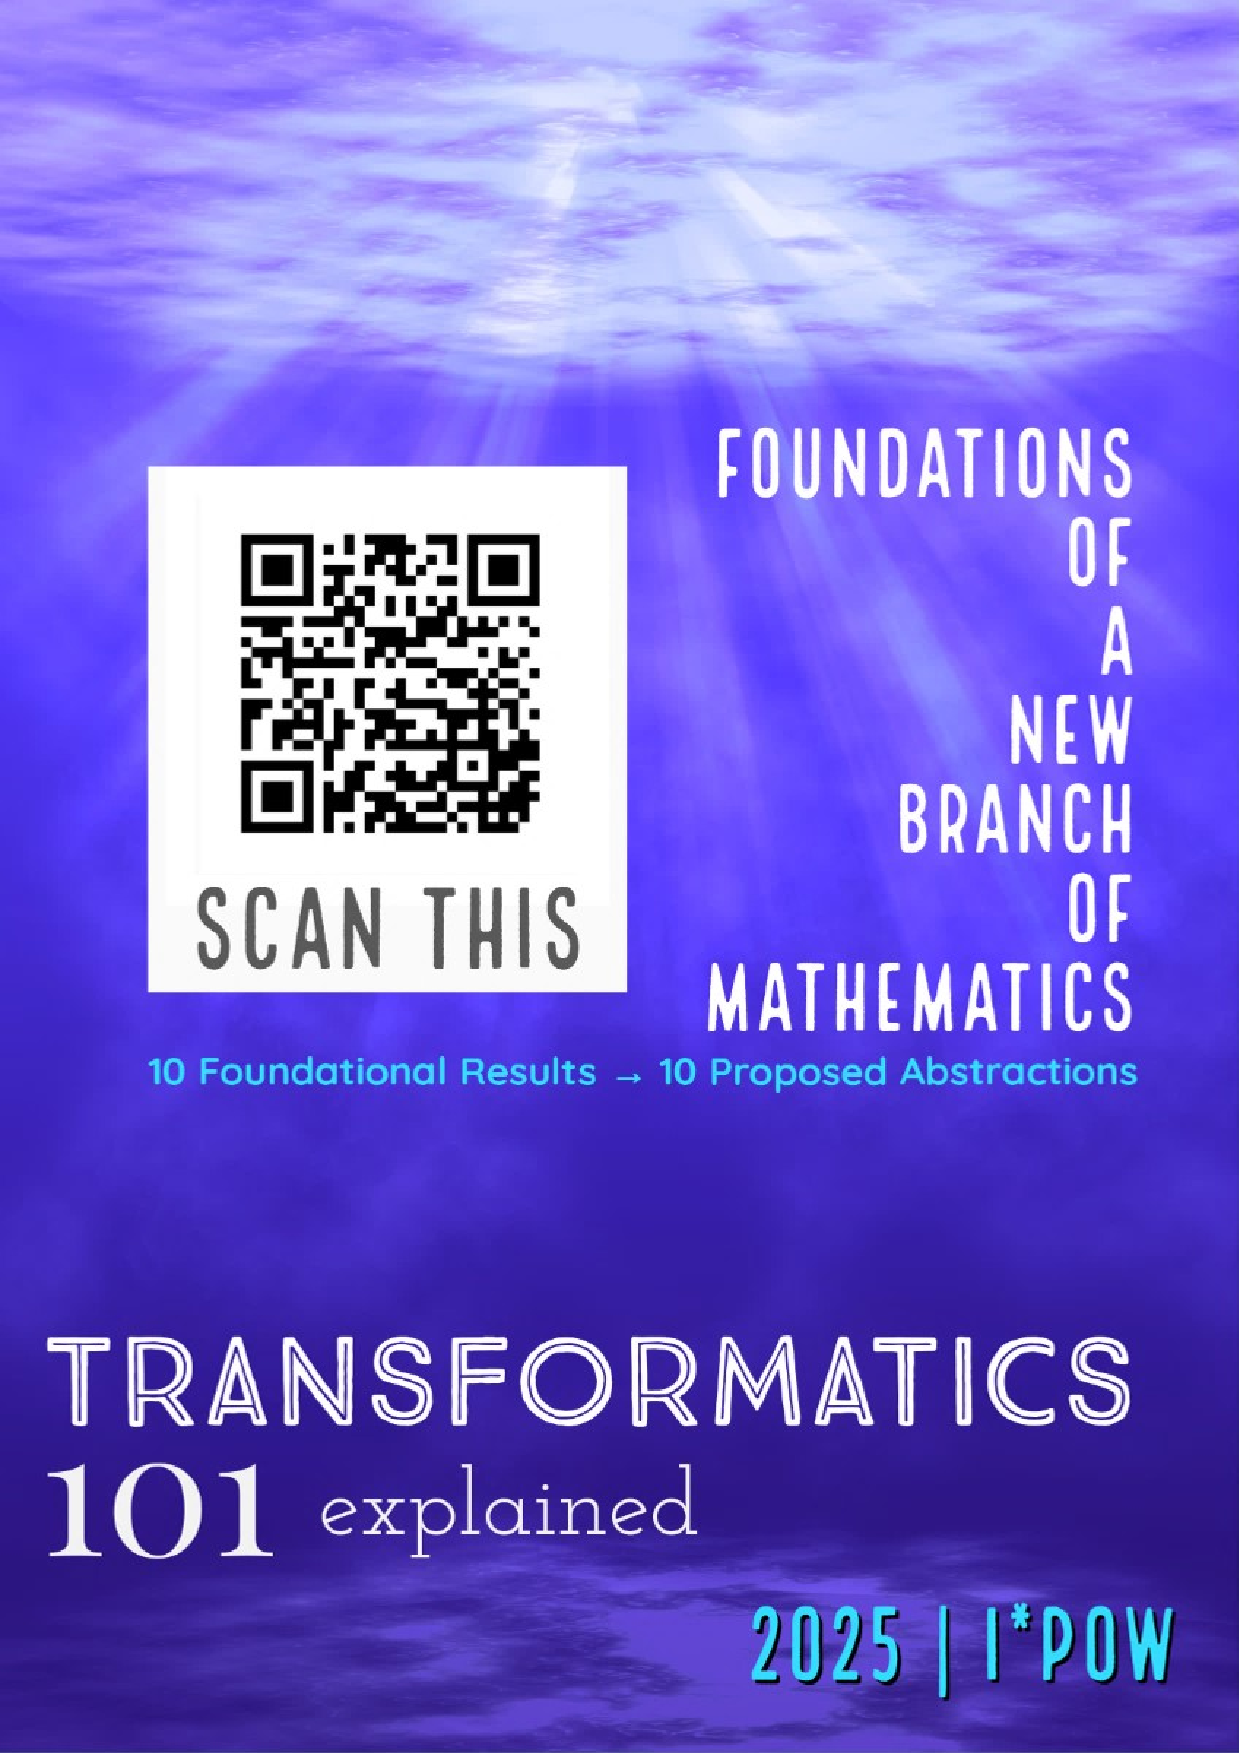
\includepdf[pages=1]{resources/pdfs/trans_back_cover.pdf}


%%%%%%%%%%%%%%%%%%%%%%%%%%%%%%%%%%%%%%[ END TRANSFORMATICS 101 ]%%%%%%%%%%%%%%%%%%%%%%%%%%%%%%


%%%%%[ EXTRA NOTE concerning Transformatics 101 ]


%draw horizontal line
%\noindent\rule{\textwidth}{0.4pt}



\chapter{Situating TRANSFORMATICS (as a Theory or Field) within Mathematics:}
\label{CHAPSITTRANS}


\section{A Working Definition and Clarification on Fundamental Nomenclature}



\vspace{2em}

\begin{defn}[\textbf{Transformatics}]
\label{DEFTRANS}
The study of \textbf{sequences of symbols}, their transformations and analysis.
\end{defn}

\vspace{2em}

To kick-start our discussion, note that the definition above shall help to distinguish transformatics as its inventor currently treats of it, from any other mathematical line of inquiry, but shall also help explain why past references to and parallels between transformatics and topics such as sequence analysis, sequence transformers, sequence generators and especially a heavy talk about symbol sets and sequences makes all the sense (refer to \textbf{\hyperref[SECFOUND]{Section \ref{SECFOUND}}}). That said, note that we are going to attempt to properly, perhaps somewhat rigorously locate this theory and associated concepts within the vast spectrum of mathematics. However, first, let us clear-up the potential confusion concerning fundamental nomenclature and potential parallels between other fields and sub-fields of mathematics.

\vspace{2em}

In keeping with standard nomenclature, but also applying it well, we shall want to help the reader, and especially the students of Transformatics, to readily distinguish between several somewhat similar, yet distinct concepts and terms from across mathematics, that might help anyone readily make sense of \textbf{\hyperref[DEFTRANS]{Definition \ref{DEFTRANS}}}. So, first, we are going to outline the distinctions and relationships between six foundational mathematical structures: \textbf{set}, \textbf{sequence}, \textbf{series}, \textbf{vector}, \textbf{matrix}, and \textbf{space}. These concepts are central to fields such as linear algebra, analysis, and symbolic systems \cite{axler2015linear, rudin1976principles}.


\section*{Comparison Table}

\begin{center}
\begin{tabular}{|l|c|c|c|l|}
\hline
\textbf{Concept} & \textbf{Ordered?} & \textbf{Duplicates?} & \textbf{Dimensionality} & \textbf{Key Feature} \\
\hline
\hline
Set & No & No & Abstract & \makecell[l]{Unordered collection\\of distinct elements}\\
\hline
Sequence & Yes & Yes & 1D & \makecell[l]{Ordered list\\indexed by $\mathbb{N}$}\\
\hline
Series & Yes & Yes & 1D & \makecell[l]{Sum of a sequence\\(often infinite)}\\
\hline
Vector & Yes & Yes & 1D (or $n$D) & \makecell[l]{Element of\\a vector space}\\
\hline
Matrix & Yes & Yes & 2D & \makecell[l]{Rectangular array\\of scalars}\\
\hline
Space & N/A & N/A & $n$D (abstract) & \makecell[l]{Set with algebraic\\or topological structure}\\
\hline
\end{tabular}
\label{TABCOMPCONCEPTS}
\end{center}

\section*{Definitions and Examples}
\label{SECDEFSTRUCTURES}

\subsection*{Set}
A \emph{set} is a collection of distinct elements with no inherent order. For example, $\{2, 3, 5\}$ is the same as $\{5, 2, 3\}$. Sets are foundational in logic and topology \cite{halmos1960naive}.

Also, and concerning formal expression, note that authors such as Patrick M. Fitzpatrick, when introducing sets in their textbook undergraduate calculus\cite{fitzpatrick1995advanced}, have this to say:


\noindent
\begin{minipage}{1\textwidth}
\vspace{1em}
\begin{quotation}
{\ttfamily

For a set \textbf{A}, the membership of the element $x$ in \textbf{A} is denoted by $x \in \textbf{A}$ or $x$ in \textbf{A}, and the nonmembership of $x$ in \textbf{A} is denoted by $x \not\in \textbf{A}$. A member of \textbf{A} is often called a \textit{point} in \textbf{A}. Two sets are the same if and only if they have the same members. Frequently sets will be denoted by braces, so that $\{ x \quad | \quad \text{proposition about x}\}$ is the set of all elements $x$ such that the proposition about $x$ is true.

}
\end{quotation}
\vspace{1em}
\end{minipage}

\vspace{2em}

That quote gives us a good introduction to the notation most commonly used to treat of sets --- a structure that in one way or another, likewise serves immensely in justifying the formalisms likewise used in transformatics. Also, note that, authors like Walter Nef, introducing sets in a linear algebra text\cite{nef1967linear}, uses a generalization somewhat merely more abstract than the plain-english version above, but still in the same vein, when he writes 


\begin{equation}
\label{EQSETNOT}
A = \{ x_1, x_2, x_3, ... \} = \{ x ; \phi(x) \}
\end{equation}

\vspace{2em}

So that $\phi(x)$ denotes a statement by which the elements of A are characterized\footnote{Walter's use of ``;"such as we depict in \textbf{\hyperref[EQSETNOT]{Equation \ref{EQSETNOT}}} might somewhat significantly differ from the notation we have heavily utilized in transformatics when we prefer to either write $\{x: \phi(x)\}$ or even just $\{x \quad|\quad \phi(x)\}$, but the semantics remain the same.}. Moreover, as we see in \textbf{\hyperref[TABCOMPCONCEPTS]{Table \ref{TABCOMPCONCEPTS}}}, particularly for \textbf{only sets}, the order of members or elements \textbf{does not matter}, and also that, \textbf{duplication is not allowed}. Thus, we see below, that we might express a set with different orderings of its members, and still correctly refer to the same set:

\begin{equation}
VOWELS = \{ a, e, i, o, u \} = \{ e, i, o, a, u \} = \{ u, o, i, e, a\} = \{x : x \in \psi_{vowels} \}
\end{equation}

\vspace{2em}

Where $\psi_{vowels}$ is the symbol set of only the 5 vowels of the Latin Alphabet.


%draw horizontal line
\noindent\rule{\textwidth}{0.4pt}


\subsection*{Sequence}
\label{DEFSEQUENCE}

A \emph{sequence}\index{sequence!definition} is an ordered list of elements possibly with repetition\cite{copilot_dna_assistant} --- for transformatics though, we many times prefer to say ``of symbols". For instance, the Fibonacci sequence is $(1, 1, 2, 3, 5, 8, \dots)$, while the sequence of the vowels in the Latin Alphabet is\footnote{We borrow the formalism of a symbol set over a set, but whose elements are ordered by some criteria, in this case, that of the latin alphabet such as in \cite{transformatics}, but also see \textbf{\hyperref[EQDNASS]{Equation \ref{EQDNASS}}}.} $\hat{\psi}_{az}(VOWELS) = \psi_{vowels}$ as depicted below:


\begin{equation}
\psi_{vowels} = \langle a, e, i, o ,u \rangle \neq \langle e, a, i, o ,u \rangle \neq \langle u, o, i, e, a \rangle
\end{equation}


 Sequences are central in analysis and recursion theory \cite{rudin1976principles}, but also are at the core of transformatics\footnote{Refer to \cite{Lutalo2025_transformatics_thesis}, \textbf{\hyperref[SECFOUND]{Section \ref{SECFOUND}}} and \textbf{\hyperref[DEFTRANS]{Definition \ref{DEFTRANS}}} among others.}.

\vspace{2em}

Note how, as in much of the recent literature on transformatics, we mostly prefer to express sequences using the notation $\langle a_1, a_2, \cdots \rangle$ and not say $\{ a_1, a_2, \cdots \}$ --- this, especially so we emphasize the fact that \textbf{order matters} in transformatics, and so we can \textbf{readily differentiate between unordered sets and ordered sets or rather sequences}. Moreover, as shown in \textbf{\hyperref[EQNASEQ]{Equation \ref{EQNASEQ}}}, we might sometimes prefer to summarize or generalize sequences using notations such as:

\vspace{2em}
For infinite sequences...

\begin{equation}
S_\infty = \langle \cdots, a_{n-1}, a_n, a_{n+1}, \cdots \rangle = \langle a_i \rangle^\infty
\end{equation} 

\vspace{2em}
And for finite sequences as...

\begin{equation}
S_n = \langle a_1, a_2, \cdots, a_{n-1}, a_n \rangle = \langle a_i \rangle^n
\end{equation} 

\vspace{2em}

For $i \in \mathbb{N}$. 

\vspace{2em}

However, and especially where we know that the elements in a sequence might not necessarily be numbers, or that they might not even be simple elements such as just literal symbols but perhaps symbolic structures of say a complex kind --- such as a sequence of codons encoding a gene or perhaps a sequence of words that define or specify a particular phrase such as the command ``fire melts ice"\footnote{Which is indeed different both literally and semantically from ``ice melts fire" or perhaps ``melts fire ice", etc.}, or perhaps, the sequence of instructions in a TEA program (refer to \textbf{\hyperref[PROP9]{Section \ref{PROP9}}}) --- in such cases, we shall want to generalize a sequence by incorporating information about the symbol set spanned by its elements. Thus, we might  adopt generalizations such as...

\vspace{2em}

\begin{equation}
S_\infty = \langle \cdots, a_{n-1}, a_n, a_{n+1}, \cdots \rangle = \langle a_i \in \psi_S \rangle^\infty
\end{equation} 

\vspace{2em}

Or perhaps

\vspace{2em}

\begin{equation}
S_n = \langle a_1, a_2, \cdots, a_{n-1}, a_n \rangle = \langle a_i \in \psi_S \rangle^n = \mathbb{N} \times \psi_S
\end{equation} 

\vspace{2em}

or, as preferred in calculus texts such as \cite{fitzpatrick1995advanced}, as..


\vspace{2em}

\begin{equation}
S_n = \langle a_1, a_2, \cdots, a_{n-1}, a_n \rangle = f: \mathbb{N} \rightarrow \psi_S
\end{equation} 

\vspace{2em}

And just $S_n = \{a_k\}$ or maybe $S_n = \{f(a_k)\}$  and even the very plain $a_n = f(n)$ as commonly used in calculus texts such as \cite{fitzpatrick1995advanced} and especially in Ron Larson et al.\cite{ronlarsoncalculus}. In these cases, the emphasis, especially because for fields such as calculus, sequences are used to treat of and generalize continuous or discrete functions mapping the counting numbers ($\mathbb{N}$) to some other numbers (especially to real numbers, $\mathbb{R}$), so that, by focusing on the general term only, and using $n$ as the common subscript in the general term, such as when the sequence of square numbers is written as $\{a^2\}$, it is understood that these collections might be finite or even infinite, however, that the key thing is how, when given any particular position index such as i=1 or i=n or i=$\infty$, one can correctly derive or compute the corresponding term within the specified sequence. In transformatics though, especially when not dealing with sequences whose terms might be readily generalizable using some simple formula that is a function of just the position index, we might prefer to use other generalization notations as the case best warrants.

\vspace{2em}

Finally, note that, perhaps out of preference and for consistency with earlier literature\cite{Lutalo2024gtnc} in transformatics and its development\cite{adtpaper}\cite{ossipaper}\cite{transformatics}, we usually depict general or arbitrary sequences using the letter Theta --- $\Theta$, and its terms or elements using the lowercase version $\theta$ such as in:

\vspace{2em}

\begin{equation}
\Theta^n = \langle \theta_i \rangle^n : \theta_i \in \psi_\beta \quad \land \quad \invpi(\Theta) = n  \quad \land \quad i,n \in \mathbb{N}
\end{equation}

\vspace{2em}

For some symbol set $\psi_\beta$ that characterizes the elements of the sequence. But, and \textbf{this is important}; as with many instances across mathematics --- which is just \textit{a language for unambiguously stating [general] truths} --- when the context is clear and simplicity is preferable, much of these formalisms and notations do get much more simpler than discussed here, and so that, to the uninitiated, sometimes it might appear as though one is saying one or more things, when in fact, a certain expression or mathematical statement is actually meaning a particular thing\footnote{As always, care, practice and the \textit{right} background knowledge is necessary when both writing and reading or analyzing mathematical texts, more so in such a new field or theory such as transformatics is.}.

%draw horizontal line
\noindent\rule{\textwidth}{0.4pt}


\subsection*{Series}

A \emph{series} is the sum of a sequence\cite{copilot_dna_assistant}, however, in drawing parallels with similar formalisms from some mathematics fields such as linear algebra, we might likewise think of series as kinds of \textbf{linear combinations}. For example:

\vspace{2em}

\begin{equation}
 Q = \sum_{n=0}^{\infty} \frac{1}{2^n} = 1 + \frac{1}{2} + \frac{1}{4} + \cdots = 2.
\end{equation}

\vspace{2em}

Depicts a series $Q$, defined as the linear combination of the terms of a sequence whose general term is $\frac{1}{2^n}$.

\vspace{2em}

Series are used in convergence analysis and power series expansions\cite{knopp1990theory}, which applications come in handy when computing limits or numerical approximations of continuous and discrete functions such as in calculus, but also, because we have related them to linear combinations in linear algebra, they likewise find varied applications in vector analysis such as in establishing linear independence, linear groups, etc \cite{nef1967linear}.

\vspace{2em}

Also, because series are somewhat conventionally derived from sequences\cite{fitzpatrick1995advanced}, such that if we have a sequence S = $\{a_k\}$, then both $\sum\limits_{k=1}^{n} a_k$ and $ \sum\limits_{k=0}^{\infty} \alpha a_k = \alpha \sum\limits_{k=0}^{\infty} a_k$ for some scalar $\alpha$ are corresponding series based off of it, one might wonder, and correctly so, is a linear combination of the terms of S via multiplication a series as well or not? Basically, if S = $\{a_1, a_2, ..., a_n\} = \{a_{i\in [1,n]}\}$, and that $\alpha_1, \alpha_2,... ,\alpha_n$ are scalars, so that

\begin{equation}
\label{EQSLINCOMBA}
S^+ = \alpha_1a_1 + \alpha_2a_2 + ... + \alpha_na_n = \sum\limits_{i=1}^{n} \alpha_i a_i  
\end{equation}

or that

\begin{equation}
\label{EQSLINCOMBB}
S^* = \alpha_1a_1 \times \alpha_2a_2 \times ... \times \alpha_na_n = \prod\limits_{i=1}^{n} \alpha_i a_i  
\end{equation}

\vspace{2em}

We know that  \textbf{\hyperref[EQSLINCOMBA]{Equation \ref{EQSLINCOMBA}}}, or rather, $S^+$ depicts a series or a linear combination over the terms of the sequence S, however, would it also be correct to refer to  \textbf{\hyperref[EQSLINCOMBB]{Equation \ref{EQSLINCOMBB}}} or rather $S^*$ as a series too? 

%draw horizontal line
\noindent\rule{\textwidth}{0.4pt}


\subsection*{Vector}

A \emph{vector} is an element of a vector space, often represented as an ordered tuple or as a sequence of sequences. Vectors are generally used to depict quantities that have both magnitude and direction\cite{axler2015linear}\cite{ronlarsoncalculus} such as velocity, momentum, and force.

\vspace{2em}

When expressing vectors, we normally want to stress the fact that they consist of one or more components, for which each component corresponds to some particular dimension or direction. For example, a pure scalar such as just the number 5, might become a vector, when it is expressed as $\overset{\rightarrow}{5}$ or $\overset{\leftarrow}{5}$ --- in which case we are combining information about direction with information about magnitude, and that our vector consists of just one component or dimension\footnote{In this case we might for example be describing the velocity of a ball swooshing past us, and are interested in indicating its speed and whether it was headed left or right, and nothing more.}.

\vspace{2em}

When a vector consists of multiple components, such as when a ball's velocity needs to describe its relative speeds in the three dimensions of space --- typically denoted $x$, $y$ and $z$, we then might want to express the vector as either a dimension oriented sequence, a dimension annotated series or as some kind of matrix (usually as a column matrix), such as in:

\vspace{2em}

\begin{equation}
\label{EQVECT}
\vec{v} = \langle 1, 3, 2 \rangle \equiv 1\textbf{x} + 3\textbf{y} + 2\textbf{z} \equiv  \begin{bmatrix} 1 \\ 3 \\ 2 \end{bmatrix} \in \mathbb{R}^3
\end{equation}


\vspace{2em}

That we can use sequences to depict vectors, such as in the first expression used to specify the vector $\vec{v}$ in the above equation might help to align some results or arguments in transformatics with other mathematical fields such as in calculus, mechanics or even linear algebra. This is essentially via the realization that, as long as we understand a vector to depict an ordered set of quantities where each position in the set maps to a particular dimension, that then, if we for example had a vector that only has two components --- e.g. a velocity with only components in the $x$ and $z$ dimension, we might then still use the sequence notation common in transformatics, to express it, such as in:


\begin{equation}
\label{EQVECT2}
\vec{v} = \langle 1, 0, 2 \rangle \equiv 1\textbf{x} + 0\textbf{y} + 2\textbf{z} = 1\textbf{x} + 2\textbf{z} \equiv  \begin{bmatrix} 1 \\ 0 \\ 2 \end{bmatrix} \in \mathbb{R}^3
\end{equation}


\vspace{2em}

Thus for example, the case of \textbf{complex numbers} ($\mathbb{C}$), that consist of a real and imaginary component, and which are generally written as the linear combination $a + i\textbf{b}$, might likewise use a sequence-like notation such as just $\langle a, b\rangle$ when the context is clear. In fact, Larson et al. in \cite{ronlarsoncalculus} in their calculus treatment of vectors in the plane has this to say:


\noindent
\begin{minipage}{1\textwidth}
\vspace{1em}
\begin{quotation}
{\ttfamily

The components of \textbf{v} = $\overset{\rightarrow}{PQ}$, where P = ($a_1$,$b_1$) and Q = ($a_2$,$b_2$), are the quantities [such that] $a = a_2 - a_1$ ($x$-component) [and] $b = b_2 - b_1$ ($y$-component), [and so that] the pair of components is denoted $\langle a, b \rangle$.

}
\end{quotation}
\vspace{1em}
\end{minipage}

\vspace{2em}

And thus, when the dimensions aspect is clear, we might sometimes see a vector written as just a sequence such as just $\langle a, b \rangle$ --- the \textbf{transformatic-way}, or perhaps as a column matrix, $\begin{bmatrix} a \\ b \end{bmatrix}$ --- the linear algebraic way.


%draw horizontal line
\noindent\rule{\textwidth}{0.4pt}


\subsection*{Matrix}

A \emph{matrix}\index{matrix!definition} is a two-dimensional array of scalars \cite{copilot_dna_assistant}. In the transformatics language though, we might think of a matrix as a higher-order sequence (see \textbf{\hyperref[PROP8]{Section \ref{PROP8}}}) --- essentially, a sequence of sequences. In fact, a more commonplace or familiar approach might be to think of a matrix as a sequence of vectors --- this helps appreciate that:

\vspace{2em}

\begin{enumerate}
\item A matrix could be reduced to a vector.
\item A matrix could be interpreted as the projection of one or more vectors to a sequence that preserves just their component magnitudes but otherwise respecting the dimensions of each component.
\item Any vector can essentially be re-written as either a column or row matrix.
\end{enumerate}


\vspace{2em}

Matrices are normally described or characterized by their dimensions, so that we find authors such as Walter Nef in \cite{nef1967linear} talking of matrices as ``a rectangular array of numbers", and that ``the matrix A has \textit{m rows} and \textit{n columns}" --- this, when talking of a structure generalized such as:


\[ A = \begin{pmatrix} \alpha_{11} & \alpha_{12} & \cdots & \alpha_{1n} \\  \alpha_{21} & \alpha_{22} & ... & \alpha_{2n} \\  \cdots & \cdots & \cdots & \cdots \\ \cdots & \cdots & \cdots & \cdots \\ \alpha_{m1} & \alpha_{m2} & \cdots & \alpha_{mn} \\ \end{pmatrix} = \alpha_{ik} \]


\vspace{2em}

Where $k = 1, 2, \cdots, n$ and $i = 1, \cdots, m$ --- essentially, $i, k \in \mathbb{N}$, and further, that ``the \textit{mn} scalars $\alpha_{ik}$ are known as the elements of the matrix", and that we refer to a matrix that \textit{m} rows and \textit{n} columns as an $m \times n$ matrix.

\vspace{2em}

Then, we also know that matrices represent linear transformations\index{matrices!as linear transformations} and systems of equations \cite{strang2016introduction}\cite{nef1967linear}, and this might be appreciated by relating the case on vectors that we saw before this, to how we might map vectors to matrices, as well as use them to express [linear] transformations. For example, assuming we have a starting vector P = $\langle 1, 2 \rangle$ and a resultant vector Q = $\langle 3, 4 \rangle$, we might then talk of the transformation $A = \overset{\rightarrow}{PQ}$ resulting from the ordered application of these two vectors as such:

\vspace{2em}

\[ A = \begin{pmatrix} \overset{\rightarrow}{P} \\ \overset{\rightarrow}{Q} \end{pmatrix} = \begin{bmatrix} 1 & 2 \\ 3 & 4 \end{bmatrix} \]

\vspace{2em}

And we would be able to reduce this matrix to a corresponding transformation vector respecting the dimensions as such:

\[ A = \begin{pmatrix} 1 & 2 \\ 3 & 4 \end{pmatrix} \begin{pmatrix} x \\ y \end{pmatrix} = \begin{pmatrix} 1\cdot x + 2\cdot y \\ 3\cdot x + 4\cdot y \end{pmatrix} = (3-1)x + (4-2)y  = 2\textbf{x} + 2\textbf{y}\]

\vspace{2em}

So that then, we essentially can express the transform $\overset{\rightarrow}{PQ}$ as just the sequence $\langle 2, 2 \rangle$.

\vspace{2em}

Finally, note that, as when we had the debate concerning whether to express sequences in transformatics using braces $\{ \cdots \}$ or instead angled brackets $\langle \cdots \rangle$, note that also, in many fields of mathematics where matrices are encountered, you shall find use of both square brackets $[ \cdots ]$, and brackets $( \cdots )$. The choice often depends on the author and the conventions in the field as long as no confusion arises, otherwise, they might be used interchangeably too.


%draw horizontal line
\noindent\rule{\textwidth}{0.4pt}

\subsection*{Space}
A \emph{space} is a set with additional structure \cite{copilot_dna_assistant}\footnote{Interesting to note: this kind of phrasing somewhat resonates with what is also typical when talking of an \textbf{algebra} --- \textit{a set with a specific operation or operations well-defined for it} --- refer to \textbf{\hyperref[SECTRANSLAG]{Section \ref{SECTRANSLAG}}} for more on this.}. Examples include:
\begin{itemize}
  \item \textbf{Vector space}: closed under addition and scalar multiplication.
  \item \textbf{Metric space}: equipped with a distance function.
  \item \textbf{Hilbert space}: complete inner product space.
\end{itemize}
Spaces provide the abstract setting for geometry, analysis, and quantum mechanics \cite{kolmogorov1970introductory}.

%draw horizontal line
\noindent\rule{\textwidth}{0.4pt}



\section{Comparison with Other Fields}

Before we close our focus on extending what was originally introduced via the Transformatics 101 thesis\cite{Lutalo2025_transformatics_thesis}, it shall especially be worth adding a word or two concerning where, across the vast spectrum of all mathematics and the mathematical disciplines and sub-disciplines, we might correctly locate or position our theory of Transfomatics. This undertaking might not be something we can fully and rigorously accomplish within the context of chapter-sub-section such as this, however, and especially for completeness's sake, it is better we attempt and kick-start this discussion here, in this vital work --- the first to undeniably non-trivially, but also exhaustively apply Transformatics (the other major works being \cite{Lutalo2025transpsy} on Psychology, \cite{Lutalo2024TEATAZ} on the TEA language, and more recently, \cite{lutalo_2025_grimlumtauto} on Western Esotericism).


\vspace{2em}

\subsection{Relation to Statistics}
\label{SECRELSTAT}

It shall be helpful to note that, earlier attempts to situate this theory within the spectrum of mathematics --- such as when we penned the paper \cite{transformatics}, mostly relied on ``bias" towards where it is that most of the developed theory at that point would find its closest relatives. Thus, it should not be so shocking that initially, we thought perhaps Transformatics had better be treated as a theory within \textbf{mathematical statistics} --- especially because, as one can tell looking at the proposed applications of the theory (\textbf{\hyperref[SECPROP]{Section \ref{SECPROP}}}), many of the proposed and developed ideas back then indeed resonated well with work in \textbf{Statistics}, and that, as with many theories and formalisms in that field, much of what makes statistics what it is, starts by the \textit{special} treatment of sequences known as \texttt{data}\footnote{Whether as ``raw data" or as ``coded data"\cite{clarke1992basic}}\index{data!coded or raw} --- such as when we treat of a variable $X$, that might taken on values $x_i$ spanning some symbol set ($\psi_X$) and ordered by the naturals ($\mathbb{N}$) --- i.e 

\begin{equation}
X = \{ x_i: i = 1, 2, ..., N\} = \{x_i : i \in \mathbb{N}\} = \psi_X \times \mathbb{N} = x_{i\in \mathbb{N}} \in \psi_X
\end{equation}

\vspace{2em}

However, and despite the fact that statistics heavily and naturally relates to not only collecting information that is then encoded using sequences, and which is then processed and interpreted as sequences (of data points, observations, events, probabilities, measurements etc), however, \textbf{it is not} the only major field of mathematics that essentially treats of structures in the form of sequences. 

\vspace{2em}

\subsection{Relation to Linear Algebra}
\label{SECRELLINALG}

The other competing field might for example be \textbf{Linear Algebra}\footnote{Majorly\cite{copilot_dna_assistant} attributed  to \textbf{Hermann Grassmann} the 19th century German polymath that first \textit{created} linear algebra in its modern form when he penned the 1844 work \textit{Die Lineale Ausdehnungslehre} (``Theory of Linear Extension") which introduced the ideas of vector spaces and linear combinations.  Other contributors\cite{copilot_dna_assistant} are Gottfried Willhelm Leibniz (1693) that introduced early ideas of matrices and determinants; Gabriel Cramer (1750) that published \textit{Cramer's Rule} for solving $n$ equations in $n$ unknowns; Joseph-Louis Lagrange (late 1700s) that used matrices to study bilinear forms, and finally Giuseppe Peano (1888) that introduced the abstract modern concept of a vector space, in essence, completing the conceptual framework that underlies all of linear algebra.}; in that field, sequences do show up right at the start (see for example Chapter 1 of \cite{nef1967linear}), and particularly, they \textit{initially} manifest in the form or under the terminology of \texttt{sets}, and then \textit{soon enough} in the [more transformatic] form of matrices of many kinds, and that, very often, much of the theory and formalisms of linear algebra rotate around encoding data as the mathematical structure known as a matrix\footnote{Which we have seen to actually be based on sequences --- refer to \textbf{\hyperref[SECDEFSTRUCTURES]{Section \ref{SECDEFSTRUCTURES}}}}, whether of a simple form such as 1-dimensional finite sequence, or as high-dimensional dense or sparse matrices encoding infinitely large spaces or quantifiably large datasets. That field also presents many processes that deal with reducing such basic or higher-order sequences\index{sequence!higher-order} (\textbf{\hyperref[PROP8]{Section \ref{PROP8}}}), also sometimes likened to or related to ``vectors", to just simple expressions or quantities such as scalars --- basic numbers in their simplest forms, via \textbf{linear-transformations} of many kinds. And talking of transformations, we find in the field of linear algebra, many kinds of ways that one sequence might be mapped or reduced to another sequence, via processes or computations such as computing the basis (a sequence from which other sequences of similar structure can be derived), endomorphisms (linear transforms that map a type onto itself), inverses (sequences which would result in the identity sequence when multiplied with the source sequence), etc.\cite{nef1967linear}

\vspace{2em}

First, concerning sequences in particular, it shall be worth noting that Walter Nef does even explicitly bring up the concept of \textit{a sequence space} --- in relation to, and derived from the concept of a real vector space (also to be found in other fields such as Calculus and real analysis), when he writes:

\vspace{2em}

\noindent
\begin{minipage}{1\textwidth}
\vspace{1em}
\begin{quotation}
\noindent {\ttfamily

Instead of ordered sets of $n$ real numbers, we can also consider countably infinite sequences of real numbers, i.e., $x = (\xi_1, \xi_2, \xi_3, \cdots )$. Addition and multiplication by scalars can be defined... term by term... and in this way, a new real vector space is constructed which we call the space of sequences

}
\hspace*{\fill} --- \textbf{Walter Nef}, \textit{Linear Algebra}, 1967\cite{nef1967linear}
\end{quotation}
\vspace{1em}
\end{minipage}

\vspace{2em}


Moreover, and not to confuse transformatics with linear algebra and similar mathematics, note that, whereas they talk of ``spaces" as especially sets or families of sets that especially satisfy the \textbf{7 axioms of a vector space}, and which especially focus on the operations of addition (of the member sets to other member sets) and multiplication (of scalars by member sets), such that then we can talk of ``the space of sequences", ``the space of polynomials", ``the space of linear manifolds", etc. in transformatics, we are more interested in not assuming anything about the nature of the elements of a set, so that for example, we might not readily talk of the possibility of a meaningful multiplication of a scalar by an element in some set, or that we might not guarantee that the axioms expected of a vector space hold when we apply them to say, sequences of letters (such as in $\psi_{az}$ or $\psi_{na}$), sequences of TEA instructions, etc. And also that, as introduced in both \cite{transformatics} and \cite{treealgebras_review}, we are more interested in operations that can be applied to sequences irrespective of the nature of the elements they contain --- for example, \textbf{concatenation}, \textbf{filtering}, \textbf{lateral inversion}, \textbf{cardinality} etc. would readily work well on sequences of real numbers, integers, letters of the latin alphabet, sequences of quaternions, etc.

\vspace{2em}

Thus, even though transformations of a linear kind or rather, ``linear transformations" in the strict sense, might correctly treat of sequences, vectors and matrices such as when we have two vectors $u$, $v$, and $z$ and some scalar $c$, so that, given some linear transformation $T: V \rightarrow W$ mapping between vector spaces, we have that:

\vspace{2em}

\begin{equation}
T(u + v) = T(u) + T(v) = z
\end{equation}

\vspace{2em}

and that

\vspace{2em}

\begin{equation}
T(cu) = cT(u)
\end{equation}

\vspace{2em}

And so that the transformation $T(\cdot)$ can be treated of as we typically do in transformatics as such:

\vspace{2em}

\begin{trans}
$u + v \xrightarrow{T} z$
\end{trans}

\vspace{2em}

And that if $T(u) = u^*$ and $T(v) = v^*$, so that $u^* + v^* = z$, then we also expect that:

\vspace{2em}

\begin{trans}
$u^* + v^* \rightarrow z$
\end{trans}

\vspace{2em}

Or to sum it all up in a linear-algebraic-transformatic notation combo\footnote{Perhaps totally bonkas!}, we have that:

\vspace{2em}

\begin{equation}
\label{EQAXIOMALG}
(u + v \xrightarrow{T} z) \equiv ((u \xrightarrow{T} u^*) + (v \xrightarrow{T} v^*) = z)
\end{equation}

\vspace{2em}

For those not very familiar with linear algebra, note that \textbf{\hyperref[EQAXIOMALG]{Equation \ref{EQAXIOMALG}}} would for example hold for transformations such as \textbf{halving} --- but not say \texttt{squaring}. For example, if we have  $u = \left[\begin{smallmatrix}3\\2\end{smallmatrix}\right]$ and $v = \left[\begin{smallmatrix}4\\5\end{smallmatrix}\right]$, and that we have the operation $T(u) = \{\frac{\alpha_{ik}}{2}\}$ for all $\alpha_{ik} \in u$, then we would indeed see that:

\vspace{2em}


\begin{multline}
\label{EQTRANSLINALG1}
T(u+v) = T\left( \begin{bmatrix}3\\2\end{bmatrix} +  \begin{bmatrix}4\\5\end{bmatrix} \right) =  T\left( \begin{bmatrix}3+4\\2+5\end{bmatrix} \right) = T\left( \begin{bmatrix}7\\7\end{bmatrix} \right) = \begin{bmatrix}\frac{7}{2}\\\frac{7}{2}\end{bmatrix} = \begin{bmatrix}3.5\\3.5\end{bmatrix}
\end{multline}


\vspace{2em}

While, we also see that


\vspace{2em}


\begin{multline}
\label{EQTRANSLINALG2}
T(u) + T(v) = T\left( \begin{bmatrix}3\\2\end{bmatrix} \right) +  T\left( \begin{bmatrix}4\\5\end{bmatrix} \right) = \begin{bmatrix}3*\frac{1}{2}\\2*\frac{1}{2}\end{bmatrix}  +   \begin{bmatrix}4*\frac{1}{2}\\5*\frac{1}{2}\end{bmatrix} = \begin{bmatrix}\frac{3+4}{2}\\\frac{2+5}{2}\end{bmatrix} = \begin{bmatrix}\frac{7}{2}\\\frac{7}{2}\end{bmatrix} = \begin{bmatrix}3.5\\3.5\end{bmatrix}
\end{multline}


\vspace{2em}

However, and keeping in mind that \textbf{linear transformations apply to the sequences item-wise}, we see that if instead we had an operation such as $S(u) = \{\alpha_{ik}^2\}$, then using the same $u$ and $v$ sequences above, we see that attempting to apply it separately to either sequence Vs applying it to their summation would result in different results as shown hereafter:


\vspace{2em}


\begin{multline}
\label{EQSQUARTRANS1}
S(u+v) = S\left( \begin{bmatrix}3\\2\end{bmatrix} +  \begin{bmatrix}4\\5\end{bmatrix} \right) =  S\left( \begin{bmatrix}3+4\\2+5\end{bmatrix} \right) = S\left( \begin{bmatrix}7\\7\end{bmatrix} \right) = \begin{bmatrix}7^2\\7^2\end{bmatrix} = \begin{bmatrix}49\\49\end{bmatrix}
\end{multline}


\vspace{2em}


\begin{multline}
\label{EQSQUARTRANS2}
S(u) + S(v) = S\left( \begin{bmatrix}3\\2\end{bmatrix} \right) +  S\left( \begin{bmatrix}4\\5\end{bmatrix} \right) = \begin{bmatrix}3^2\\2^2\end{bmatrix}  +   \begin{bmatrix}4^2\\5^2\end{bmatrix} = \begin{bmatrix}9+16\\4+25\end{bmatrix} = \begin{bmatrix}25\\29\end{bmatrix}
\end{multline}


\vspace{2em}

And so that for the case of a squaring transform applied linearly, we fail to meet the requirements that typical transformations are expected of in linear algebra. Or rather that...


\vspace{2em}

\begin{equation}
\label{EQAXIOMALG2}
(u + v \xrightarrow{S} z) \not\equiv ((u \xrightarrow{S} u^*) + (v \xrightarrow{S} v^*) = z^*)
\end{equation}


\vspace{2em}



It should be worth noting that for transformatics --- such as when we have the squaring transformer defined as such:

\vspace{2em}

\begin{transf}[\texttt{squaring transform}, $S(\Theta)$]
\label{TRANSSQUAR}
$\Theta^n \xrightarrow{S(\Theta)} \Theta^*;$\\
$\invpi(\Theta^n) = \invpi(\Theta^*) = n$\\
$\land \quad \forall \theta_i \in \Theta \quad \exists \theta_i^* \in \Theta^* : \theta_i^* = \theta_i^2 \quad \forall i \in [1,n]$\\
$\land \quad \theta, \theta^* \in \mathbb{R} \quad \forall \theta \in \Theta \quad \land \quad \theta^* \in \Theta^*$
$\qed$
\end{transf}

\vspace{2em}

\textbf{\hyperref[TRANSSQUAR]{Transformer \ref{TRANSSQUAR}}} would work on sequences of [real] numbers such as we see in \textbf{\hyperref[EQSQUARTRANS1]{Equation \ref{EQSQUARTRANS1}}} and \textbf{\hyperref[EQSQUARTRANS2]{Equation \ref{EQSQUARTRANS2}}}.




\vspace{2em}


So that it starts to surely become clearer that though we might somewhat relate transformatics to linear algebra (perhaps by the fact that they both treat of sequences and transformations on them)... \textbf{AND YET, THEY REALLY ARE DIFFERENT!} First, since for transformatics we ``care less"\footnote{Across a field such as Linear Algebra, it is typically expected or perhaps assumed that the structures being dealt with are at minimum, ones consisting of numbers --- they might be integers, complex numbers or real numbers, but at least they are numbers --- meaning, the transformations and operations being dealt with generally concern taking things like the sign and quantity of the number or symbol into consideration. However, Transformatics can also deal with sequences of unquantifiable symbols such as elements of the set $\psi_{DNA}$ that we encountered in \textbf{\hyperref[DEFDNASS]{Defition \ref{DEFDNASS}}}.} about the actual types of the elements of a set or sequence\footnote{Especially because, where a transformation must rely upon or have the types of the sequence elements in consideration, then the necessary conditions constraining what the transformation can apply to or not, are typically specified as part of the transformation/transformer definition or specification --- such as the final specification line in \textbf{\hyperref[TRANSSQUAR]{Transformer \ref{TRANSSQUAR}}}.}, and more on the structure [and overall composition] of the sequence \textit{before and after the transformation}, and as for the elements themselves, perhaps mostly care about properties such as whether or not they belong to some symbol set or not --- pre- and post-transform, etc. And that we can treat of sequences of elements whose types are not numbers (not just real numbers or integers as fields such as linear algebra and calculus especially focus on), so that, if we have transformatic operations such as the \textbf{Mirror} operation\footnote{Also ``lateral inversion" --- refer to \cite{transformatics}, \cite{Lutalo2024TEATAZ}, but also \cite{lutalo_2025_grimlumtauto}}, $M(\cdot)$, which, when given some sequence such the phrase ``star", returns it reflection as ``rats", so that we essentially have:

\vspace{2em}

\begin{trans}
$\langle s, t, a, r \rangle \xrightarrow{M} \langle r, a, t, s \rangle$
\end{trans}

\vspace{2em}

And that if we had two sequences, $u = \langle s, t, a, r \rangle$ and $v = \langle n, u, t, s  \rangle$, then, applying this operation to them individually, and then to their summation or concatenation might not work as one might expect when dealing with linear algebraic transforms:

\vspace{2em}


\begin{equation}
M(u) = M(\langle s, t, a, r \rangle) = \langle r, a, t, s \rangle = u^*_1
\end{equation}

\vspace{2em}

and that

\vspace{2em}

\begin{equation}
M(v) = M(\langle n, u, t, s  \rangle) = \langle s, t, u, n \rangle = v^*_1
\end{equation}

\vspace{2em}

and that

\vspace{2em}

\begin{equation}
M(u) + M(v) = u^*_1 + v^*_1 = \langle r, a, t, s \rangle + \langle s, t, u, n \rangle = \langle r, a, t, s, s, t, u, n \rangle = u^*_1v^*_1
\end{equation}

\vspace{2em}

But that

\vspace{2em}


\begin{multline}
M(u + v) = M(\langle s, t, a, r \rangle + \langle n, u, t, s  \rangle) =\\ 
 M(\langle s, t, a, r, n, u, t, s  \rangle) = \langle s ,t ,u ,n ,r ,a ,t ,s \rangle = v^*_1u^*_1
\end{multline}

\vspace{2em}

So that then, unlike linear transformations, we see that for the case of transformations such as $M(\cdot)$, we have:

\vspace{2em}

\begin{equation}
M(u + v) \neq M(u) + M(v) 
\end{equation}

\vspace{2em}

Or if we are to use an approach similiar to what we saw in \textbf{\hyperref[EQAXIOMALG]{Equation \ref{EQAXIOMALG}}}:

\vspace{2em}

\begin{equation}
\label{EQAXIOMMIRROR}
(u + v \xrightarrow{M} v^*_1u^*_1) \not\equiv ((u \xrightarrow{M} u^*_1) + (v \xrightarrow{M} v^*_1) =  u^*_1v^*_1)
\end{equation}

\vspace{2em}

In fact, for the mirror operation, it is as if $M(u + v) = M(M(u) + M(v))$, which ``totally" makes the kind of operations treated of in transformatics \textbf{so unlike what one would find in linear algebra}\footnote{We say ``so unlike" and not ``totally unlike" because, as one might find, and this not to come off as a total surprise, linear transformations that are typical of linear algebra --- such as what we saw in \textbf{\hyperref[EQTRANSLINALG1]{Equation \ref{EQTRANSLINALG1}}} and \textbf{\hyperref[EQTRANSLINALG2]{Equation \ref{EQTRANSLINALG2}}}, despite being ``linear algebraic" since they conform to the requirements of vector spaces and linear transforms, are also tractable under the transformatics umbrella because nonetheless, they apply to sequences [and also result in sequences!] and that we can use the transformatics formalisms of transformers to specify and analyze them.} despite both fields treating of sequences.

\vspace{2em}

Further, and interestingly, the failure for the mirror operation to preserve the axioms of vector spaces would likewise remain the same even when we were to apply it to sequences of real numbers or numbers for that matter, and it it not the only kind of \textit{peculiar} operation or transformation that we might come across when working with sequences in transformatics --- others, such as the \textbf{LOMT: Multiplication by Lexical Order} transformation first introduced in \cite{transformatics} might likewise fail these tests!


\vspace{2em}

Finally, before we leave linear algebra, it shall be worth noting that the transformer concept in transformatics might also be likened to the concept of \textbf{mappings}\index{transformatics!mappings} in linear algebra (and from there, to other fields including calculus for example\footnote{\cite{fitzpatrick1995advanced} has an entire chapter dedicated to approximating nonlinear mappings by linear mappings for example.}). So, how would this work?

\vspace{2em}


First, note that, across many fields of mathematics where we encounter functions, the signature of a function --- also technically equivalent to a mapping, is expressed using the notation: $f : D \rightarrow R$, which we can read as ``the function $f$ maps every element in the domain $D$ to a corresponding value in the range $R$". Typically, the language used is that of sets, such as we see in the following excerpt from \cite{nef1967linear}:


\vspace{2em}

\noindent
\begin{minipage}{1\textwidth}
\vspace{1em}
\begin{quotation}
\noindent {\ttfamily

\textbf{General Mappings:}\index{mappings} Let $E$ and $F$ be two sets. A \textit{mapping of E into F} is a rule which assigns to each element $x \in E$ a unique element $y \in F$.\\

The element $y \in F$ which is assigned to the element $x \in E$ by the mapping $f$ is called the \textit{image} of $x$ under $f$ and is denoted by $f(x)$. The set $E$ is called the \textit{domain} of $f$ and $F$ is called the \textit{range} of $f$.

}
\hspace*{\fill} --- \textbf{Walter Nef}, \textit{Linear Algebra}, 1967\cite{nef1967linear}
\end{quotation}
\vspace{1em}
\end{minipage}

\vspace{2em}


And to help stress the possibility that we could actually express mappings in linear algebra using the new formalism of transformers, note how he goes on to clarify concerning the notation used to express mappings:



\vspace{2em}

\noindent
\begin{minipage}{1\textwidth}
\vspace{1em}
\begin{quotation}
\noindent {\ttfamily

Mappings will usually be denoted by small Roman letters $f$, $g$, ... \\
When an element $x \in E$ goes into the element $y \in F$ under the mapping $f$, this will be indicated by the notation $x \rightarrow y = f(x)$.

}
\hspace*{\fill} --- \textbf{Walter Nef}, \textit{Linear Algebra}, 1967\cite{nef1967linear}
\end{quotation}
\vspace{1em}
\end{minipage}

\vspace{2em}


In transformatics, we would generally express such [mappings] concepts as such:

\vspace{2em}



\begin{transf}
\label{TRANSFMAPPINGS}
$ x \xrightarrow{f(x)} y;$\\
$ x \in E \quad \land \quad y \in F$
$\qed$
\end{transf}

\vspace{2em}

So that, where we have been talking of a transformer (in transformatics), we might then talk of a mapping\index{transformatics!mappings}\index{transformer!as mapping} (or a function) in linear algebra and other related or derivative fields. Also, note that, when studying the structure of a [lean] transformer such as \textbf{\hyperref[TRANSFMAPPINGS]{Transformer \ref{TRANSFMAPPINGS}}} and comparing it to typical transformers in transformatics such as \textbf{\hyperref[TRANSSQUAR]{Transformer \ref{TRANSSQUAR}}} or perhaps a more involved case such as \textbf{\hyperref[TRANSFDECTONASEQ]{Transformer \ref{TRANSFDECTONASEQ}}}, that we typically prefer to flesh-out the transformer definition with some vital details about not just the types or character of the source and resultant (domain and range in this case), but also those essential details about the mapping/function itself --- $f(x)$ in this case --- so that, where it makes sense, we eliminate any ambiguity concerning how the elements in the source (domain) are transformed into the elements in the result (image/range). Thus, as see see in a case such as \textbf{\hyperref[TRANSFGEOSERIES]{Transformer \ref{TRANSFGEOSERIES}}} covered in the next section, we sometimes gain much by investing in a more rigorous specification of the specifics of the transformer that underlies the mapping being defined. However, it remains to be rigorously established if indeed, all \textit{transformatic mappings} are merely another kind of linear algebraic mapping.



\subsection{Relation to Calculus}
\label{SECRELCALCULUS}

And then we encounter sequences and especially [linear] sequence transformations, when dealing with sequence-based mathematical structures known as series. Concerning this, note that Sequences and Series are especially commonplace in texts and mathematics dealing with Calculus such as \cite{ronlarsoncalculus}, \cite{fitzpatrick1995advanced} and \cite{Grossman1986CalculusOneVariable} to name a few. Moreover, and as laid out in \cite{Grossman1986CalculusOneVariable}, when sequences are treated of in calculus, it is mostly, or especially in the context of ``sequences of numbers"\footnote{In fact, especially as ``sequence of real numbers", for which  \cite{fitzpatrick1995advanced} says ``A sequence of real numbers is a real-valued function whose domain is the set of natural numbers", and which he generalizes as $f:\mathbb{N} \rightarrow \mathbb{R}$, but which we might also understand to be $f: \mathbb{N} \times \mathbb{R}$ when we wish to emphasize the fact that the sequence is otherwise reducible to set of pairs where for each natural number [position] index, there is a corresponding real number --- this later notation is more common in our transformatics literature.} as we see when he says:


\noindent
\begin{minipage}{1\textwidth}
\vspace{1em}
\begin{quotation}
{\ttfamily

\textbf{Definition 1} SEQUENCE: A \textbf{sequence} of real numbers is a function whose domain is the set of positive integers. The values taken by the function are called \textbf{terms} of the sequence.\\

\textbf{NOTATION}. We will often denote the terms of a sequence by $a_n$. Thus, if the function given by Definition 1 is $f$, then $a_n = f(n)$. With this notation, \textit{we can denote the set of values taken by the sequence by $\{a_n\}$}...\\

The following are sequences of real numbers:\\

\textbf{(a)} $\{a_n\} = \begin{Bmatrix}\frac{1}{n}\end{Bmatrix}$\\ 

\textbf{(b)} $\{a_n\} = \begin{Bmatrix}\sqrt{n}\end{Bmatrix}$\\ 

...\textbf{(e)} $\{a_n\} = \begin{Bmatrix}\frac{e^n}{n!}\end{Bmatrix}$\\ 

We sometimes denote a sequence by writing out the values $\{ a_1, a_2, a_3, \cdots \}$. 

}
\hspace*{\fill} ---\textbf{Stanley I. Grossman}, \textit{Calculus of One Variable}, 1986\cite{Grossman1986CalculusOneVariable}
\end{quotation}
\vspace{1em}
\end{minipage}

\vspace{2em}


And so, we see that first of all, the notation used to denote or represent sequences in transformatics [thus far] is somewhat significantly different from that used in calculus. But this is not all concerning how we might relate treatment of sequences in transformatics with sequences in calculus. It shall be worth noting that in our formal definitions of the subject (see \textbf{\hyperref[DEFTRANS]{Definition \ref{DEFTRANS}}}, but also \textbf{\hyperref[DEFTRANS2]{Definition \ref{DEFTRANS2}}}), an explicit focus is placed on ``transformation" --- particularly, we are specially concerned with how sequences get to be mapped either to other sequences or other mathematical structures and objects, such as reducing a sequence to some number, and this is where the next contrast between transformatics and calculus comes in.

\vspace{2em}


In \textbf{\hyperref[SECDEFSTRUCTURES]{Section \ref{SECDEFSTRUCTURES}}}, we introduced the notion of the mathematical concept of series, and we noted that, it is conventionally the notion of taking a sequence (especially for calculus, a sequence of real numbers), and reducing it to some number via a finite or infinite summation of its terms starting from some index\cite{ronlarsoncalculus}\cite{Grossman1986CalculusOneVariable}. In our cross-domain explorations, we found that we might likewise think of series as a kind of application of linear combinations (a concept more common in Linear Algebra), however, this perhaps need be taken with a grain of salt\footnote{For one, linear combinations might involve the summation of terms of one or more sequences, however, there is no guarantee that the combination always needs be via addition operation alone --- yet for series, summation is the de facto signature. Also, with series, the sequences are typically of a kind where all the terms assume a general, similar form, so that the series is reducible to a formulation involving or based on just the general term and otherwise the start and end indices, whereas for linear combinations, the sequences involved might not necessarily have elements conforming to some particular structure, and thus, where summation needs be done, it might not be possible to merely derive the final/limit values without treating of each term individually, etc. But overall, and generally, it is agreed that the [infinite] series treated of in calculus are indeed linear\cite{ronlarsoncalculus}.}.. 


\vspace{2em}


So, where in transformatics we might reduce a sequence to another sequence or to some scalar, a number or some symbolic expression\footnote{For example the kind of transforms treated of in this book in \textbf{\hyperref[SEC4]{Chapter \ref{SEC4}}}, involving transformation from DNA/na-Sequences into decimal-Sequences, then to ozin-expressions and finally into Lu-Genome Expressions that have entirely little to do with the original sequence forms!}, in fields like calculus, the emphasis is on mapping sequences of numbers to some real number [only] as we see explained in these excerpts:

\vspace{2em}

\noindent
\begin{minipage}{1\textwidth}
\vspace{1em}
\begin{quotation}
{\ttfamily

\textbf{Definition 1} INFINITE SERIES: Let $\{a_n\}$ be a sequence. Then the infinite sum\\

\begin{equation}
\label{EQINFISERIES}
\sum\limits^\infty_{k=1} a_k = a_1 + a_2 + a_3 + \cdots + a_n + \cdots
\end{equation}

is called an \textbf{infinite series} (or, simply, \textbf{series}). Each $a_k$ in \textbf{\hyperref[EQINFISERIES]{Equation \ref{EQINFISERIES}}} is called a \textbf{term} of the series. The \textbf{partial sums} of the series are given by\\

\begin{equation}
S_n = \sum\limits^n_{k=1} a_k
\end{equation}


The term $S_n$ is called the \textbf{$n$th partial sum} of the series. If the sequence of partial sums $\{S_n\}$ converges to $L$, then we say that the infinite series $\sum\limits^\infty_{k=1} a_k$ \textbf{converges} to $L$, and we write\\

\begin{equation}
\sum\limits^\infty_{k=1} a_k = L
\end{equation}

Otherwise, we say that the series  $\sum\limits^\infty_{k=1} a_k$ \textbf{diverges}.

}
\hspace*{\fill} ---\textbf{Stanley I. Grossman}, \textit{Calculus of One Variable}, 1986\cite{Grossman1986CalculusOneVariable}
\end{quotation}
\vspace{1em}
\end{minipage}

\vspace{2em}


And then \cite{ronlarsoncalculus} also has this to say, concerning how a sequence's indices might be utilized when dealing with these series:


\vspace{2em}

\noindent
\begin{minipage}{1\textwidth}
\vspace{1em}
\begin{quotation}
{\ttfamily

Infinite series may begin with any index. For example,\\

\begin{equation}
\sum\limits^\infty_{n=3} \frac{1}{n} = \frac{1}{3} + \frac{1}{4} + \frac{1}{5} + \cdots
\end{equation}

When it is not necessary to specify the starting point, we write simply $\sum a_n$. Any letter may be used for the index. Thus, we may write $a_m$, $a_k$, $a_i$, etc.

}
\hspace*{\fill} ---\textbf{Ron Larson and Bruce H. Edwards}, \textit{Calculus}, 2012\cite{ronlarsoncalculus}
\end{quotation}
\vspace{1em}
\end{minipage}

\vspace{2em}


And emphasizing the fact that infinite series can be reduced to finite series (the ``partial sums"), perhaps to some limit when the underlying sequence converges, is illustrated in the result below taken from \cite{fitzpatrick1995advanced}:


\begin{equation}
\sum\limits^\infty_{k=1} a_k = \lim_{n \to \infty} \left[ \sum\limits^n_{k=1} a_k \right]
\end{equation}


\vspace{2em}


And so, overall, we find that sequence transformations in calculus are of this kind --- as series, and which essentially consist in taking finite or infinite sequences of numbers and reducing them to some particular number (a summation of the terms in the sequence). Also, it is worth noting that, even though the notations might vary, and yet, the idea of taking a sequence and mapping it to some different value, using the transformatics notations and formalisms, but yet reflecting the formulations typical of such treatments in calculus can be exemplified by the following result (the \textbf{Geometric Sum Formula}) from \cite{fitzpatrick1995advanced}, and which we then re-write as a transformatics transformer thereafter:

\vspace{2em}

\begin{equation}
\label{EQGEOMSERIES}
\sum\limits^n_{k=0} r^k = \frac{1 - r^{n+1}}{1 - r} \quad \forall r \in \mathbb{R}
\end{equation}

\vspace{2em}

Which, in transformatics we can express as the following [more generalized\footnote{Especially for completeness' sake, and to capture all the peculiarities around this important result and series as captured in different calculus texts such as \cite{ronlarsoncalculus},  \cite{fitzpatrick1995advanced} and \cite{Grossman1986CalculusOneVariable} that we have reviewed.}] transformer:


\vspace{2em}

\begin{transf}[The \textbf{Generic Geometric Series Sum Generator}, $gsum(\cdot)$]
\label{TRANSFGEOSERIES}
$ $\\
$\Theta = \langle \theta_i \rangle^n : \mathbb{N} \times \mathbb{R} \xrightarrow{gsum(\Theta)} \Theta^*;$\\
$\invpi(\Theta) = n \quad \land \quad \theta_i = cr^i \quad \forall \theta_i \in \Theta, \forall i \in [1,n] \quad \land \quad n \in \mathbb{N} \quad \land \quad r,c \in \mathbb{R}$\\
$\land \quad \Theta^* \in \mathbb{R} \quad \land \quad \Theta^* = \begin{cases}
gsum(\Theta) =  \sum\limits^{\invpi(\Theta)}_{\forall \theta_i \in \Theta} \theta_i = \sum\limits^n_{i=1} cr^i   = \frac{c(1 - r^{n+1})}{1 - r} & \forall n \geq 1 \\
1 & n = 0\\
\emptyset & r = 0 \lor r = 1
\end{cases}$\\
$\land \quad  c \quad \text{is a constant, while } \quad r \quad \text{is the common ratio.}$\\
$\qed$.
\end{transf}
 
 

\vspace{2em}


And so, the attractiveness of transformatics when compared to calculus might be appreciated by the level of detail involved in rigorously specifying an important result such as the \textbf{geometric series summation} as depicted in \textbf{\hyperref[TRANSFGEOSERIES]{Transformer \ref{TRANSFGEOSERIES}}}\footnote{In fact, and no pun intended, but this is a great example of how Transformatics might be applied in Calculus!}. The power of the transformer formalism is that, not just the core formulation of the series is specified, but all possible corner cases can likewise be catered for in a single formula, and that we can clarify on what [necessary] conditions and types all the various parameters and variables involved are or need to be so as to allow for a meaningful computation\footnote{And here is especially where transformatics shines --- leaving no loopholes when a mathematical formalism or model needs to be applied or translated into a computable solution. It is as if, these transformatics specifications are a kind of computer program expressed using pure mathematics.} of the series when given some originating sequence. Also, concerning that transformer, note that we refer to it as a ``generator" in the title, to emphasize the fact that in transformatics (as depicted in both \textbf{\hyperref[RES9]{Foundational Result 9}} and in \cite{lutalo2025transformatic}), often, we encounter \textit{special} transformers that also happen to be a kind of \textbf{generator} as explained in the transformatics literature\footnote{For example, where the calculus formulation depicted in \textbf{\hyperref[EQGEOMSERIES]{Equation \ref{EQGEOMSERIES}}} fails to make sense for parameters such as when $r=0$, or when the sequence being evaluated is empty, we find that our \textbf{\hyperref[TRANSFGEOSERIES]{Transformer \ref{TRANSFGEOSERIES}}} would otherwise still be able to return some meaningful result --- including returning the empty set, $\emptyset$, when the formula can't be meaningfully applied --- a creative way to help deal with problematic scenarios in calculus such as having to resolve results like the \textbf{indeterminate form} $\frac{0}{0}$ concerning which, mathematical history\cite{Grossman1986CalculusOneVariable} tells us the powerful Bishop George Berkeley attacked Isaac Newton's methods such as his \textit{fluxions}, and that it is another British mathematician, Collin Maclaurin (considered the finest after Newton's generation, and after whom we have \textit{Maclaurin Series}), that intervened to help save Newton's work!}.


\vspace{2em}

Finally, and revisiting the concept of mappings that we have encountered in \textbf{\hyperref[SECRELLINALG]{Section \ref{SECRELLINALG}}} when dealing with linear algebra, note that these notions come up again and again in calculus texts too, and so, we might give them some attention here as well.

\vspace{2em}


\textbf{Larson Edwards et al.} in \cite{ronlarsoncalculus} bring this concept up when discussing problems in calculus that require or call for \textit{change of variables} --- basically, the idea that many functions and analysis problems are simplified significantly when instead of working on them in their original formulations and reference frames, we instead develop some clever or useful substitution formulae that can help map the original expressions to alternative formulations that can then be tackled more directly or using more common methods. These authors introduce the concept as such:


\vspace{2em}

\noindent
\begin{minipage}{1\textwidth}
\vspace{1em}
\begin{quotation}
{\ttfamily

A function $G: X \rightarrow Y$ from a set $X$ (the domain) to another set $Y$ is often called a \textbf{map} or a \textbf{mapping}. For $x \in X$, the element $G(x)$ belongs to $Y$ and is called the \textbf{image} of $x$. The set of all images $G(x)$ is called the image or \textbf{range} of $G$. We denote the image by $G(X)$.

}
\hspace*{\fill} ---\textbf{Ron Larson and Bruce H. Edwards}, \textit{Calculus}, 2012\cite{ronlarsoncalculus}
\end{quotation}
\vspace{1em}
\end{minipage}

\vspace{2em}


Again, to relate this to how we would express mappings using the concept of transformers in transformatics, we would use a transformer definition such as:


\vspace{1em}

\begin{transf}
\label{TRANSFMAPPINGSCALC}
$ x \xrightarrow{G(\cdot)} G(x);$\\
$ x \in X \quad \land \quad G(x) \in Y$\\
$\land \quad G(X) = Y$
$\qed$
\end{transf}

\vspace{1em}


It shall of course be interesting to compare \textbf{\hyperref[TRANSFMAPPINGSCALC]{Transformer \ref{TRANSFMAPPINGSCALC}}} based on the notion of mappings as expressed in a calculus text, to \textbf{\hyperref[TRANSFMAPPINGS]{Transformer \ref{TRANSFMAPPINGS}}} based on related notions in a linear algebra text. Also, note that not all calculus texts explicitly call out transformations nor mappings. For example, in \cite{Grossman1986CalculusOneVariable}, one comes as close to the above ideas of using mappings to effect expression simplifications as the use of the idea of \textbf{variable substitution} that they then apply to simplifying problems in differentiation such as in:


\noindent
\begin{minipage}{1\textwidth}
\vspace{1em}
\begin{quotation}
{\ttfamily

If $u$ is a differentiable function of $x$, then 

\begin{equation}
\label{EQNDIFFSUBST}
\frac{d}{dx} \cos(u) = - \sin(u) \frac{du}{dx}
\end{equation}


Let $u = \sqrt{x}$. Then $du/dx$ = $1/2\sqrt{x}$, and, using \textbf{\hyperref[EQNDIFFSUBST]{Equation \ref{EQNDIFFSUBST}}}, we have\\

\[\frac{d}{dx} \cos(\sqrt{x}) = \frac{d}{dx} \cos(u) = -\sin(u)\frac{du}{dx} = (-\sin(\sqrt{x}))(\frac{1}{2\sqrt{x}}) = \frac{-\sin(\sqrt{x})}{2\sqrt{x}}\]

$\qed$\\
}
\hspace*{\fill} ---\textbf{Stanley I. Grossman}, \textit{Calculus of One Variable}, 1986\cite{Grossman1986CalculusOneVariable}
\end{quotation}
\vspace{1em}
\end{minipage}

\vspace{2em}

And we also encounter this kind of usage when simplifying integrations such as in:



\noindent
\begin{minipage}{1\textwidth}
\vspace{1em}
\begin{quotation}
{\ttfamily

Compute $\int dx/(ax +b)$.\\

\textbf{Solution.} Let $u = ax + b$. Then $du = a dx$ and\\

\[\int \frac{dx}{ax + b} = \frac{1}{a} \int \frac{a dx}{ax + b} = \frac{1}{a} \int \frac{du}{u} = \frac{1}{a} \ln |u| + C\]

or\\

\[\int \frac{dx}{ax + b} = \frac{1}{a} \ln |ax + b| + C\]

$\qed$\\
}
\hspace*{\fill} ---\textbf{Stanley I. Grossman}, \textit{Calculus of One Variable}, 1986\cite{Grossman1986CalculusOneVariable}
\end{quotation}
\vspace{1em}
\end{minipage}

\vspace{2em}


In these last two cases, we might [perhaps remotely] talk of ``simplification of solutions via transformation", and might express the ideas expressed using a transformatic notation for the last case involving integration as such:

\vspace{2em}

\begin{trans}
\label{TRANSINTEGRAL}
$\int \frac{dx}{ax + b} \xrightarrow{ax + b=u} \frac{1}{a} \int \frac{du}{u} = \frac{1}{a} \ln |u| + C   \xrightarrow{u=ax + b}  \frac{1}{a} \ln |ax + b| + C$
\end{trans}


\vspace{2em}



And then, last but not least, note that, when we still are dealing with the idea of mappings, we do encounter cases in calculus that somewhat relate to the solving of complex problems using the \textbf{chaining of transformers} or rather, the chaining of transformations. \textbf{\hyperref[TRANSINTEGRAL]{Transformation \ref{TRANSINTEGRAL}}} already exemplifies this idea for problems in calculus, however, refer to instances such as \textbf{\hyperref[TRANSF3]{Transformer \ref{TRANSF3}}} that we covered in GENETICS for the specification of a \textbf{Ribosome}, or perhaps refer to \textbf{\hyperref[PROP9]{Section \ref{PROP9}}}) that formalizes the idea of approaching computer programs as compositions leveraging chaining of sequence transformers. Overall, one would find that, the more traditional concept that relates to all of these transformatics formalisms is that of \textbf{function composition} --- or perhaps ``compositions of mappings".

\vspace{2em}

Concerning the treatment of compositions in calculus, we have the following illuminating definition from Fitzpatrick's book \cite{fitzpatrick1995advanced}:



\noindent
\begin{minipage}{1\textwidth}
\vspace{1em}
\begin{quotation}
{\ttfamily

\textbf{Definition.} For functions $f:D \rightarrow \mathbb{R}$ and $g:U \rightarrow \mathbb{R}$ such that $f(D)$ is contained in $U$, we define the composition of $f:D \rightarrow \mathbb{R}$ with $g:U \rightarrow \mathbb{R}$, denoted by $g \odot f:D \rightarrow \mathbb{R}$, by the formula\\

$(g \odot f)(x) \equiv g(f(x))$ for all $x$ in $D$. 

}
\hspace*{\fill} ---\textbf{Patrick M. Fitzpatrick}, \textit{Advanced Calculus: A Course in Mathematical Analysis}, 1995\cite{fitzpatrick1995advanced}
\end{quotation}
\vspace{1em}
\end{minipage}

\vspace{2em}

And so that, if we are to attempt to express the notion of composition as Fitzpatrick depicts above, but instead using the notation and methods of transformatics, we would process in a manner similar to what we did in \textbf{\hyperref[TRANSINTEGRAL]{Transformation \ref{TRANSINTEGRAL}}}, but more so, as we did in \textbf{\hyperref[TRANSTEAPROG]{Transformation \ref{TRANSTEAPROG}}} that indeed demonstrates the concept of composing \textbf{higher-order transformers} via the method of chaining basic transformes (in this case, functions or just mappings) back to back, and so that, we would rewrite his definition's core concept as such:


\begin{transf}[\textbf{Function Composition}, $g(f(x))$]
\label{TRANSFFUNCOMPOS}
$ $\\
$ x \xrightarrow{g(f(x))} y^* \quad \equiv \quad x \xrightarrow{f(x)} y  \xrightarrow{g(y)} y^*;$\\
$x \in D \quad \land \quad y \in U \quad \land \quad y^* \in \mathbb{R}$
$\land \quad f:D \rightarrow \mathbb{R} \quad \land \quad g:U \rightarrow \mathbb{R}$
$\qed$
\end{transf}


\vspace{2em}

The very exciting thing about this concept depicted in \textbf{\hyperref[TRANSFFUNCOMPOS]{Transformer \ref{TRANSFFUNCOMPOS}}}, and which as we have seen is essentially the traditional mathematics idea of function compositions, is that without any lying about it, is essentially what underlies the method of using TEA programs to solve arbitrary problems. We for example can see this notion at work in \textbf{\hyperref[LSTSCGEN]{Listing \ref{LSTSCGEN}}}, but also in more GENETICS-related cases such as shown in \textbf{\hyperref[SECFANAL]{Section \ref{SECFANAL}}} when we use a TEA program to compute the sequence characteristic of some DNA sequence held in a flat text file.

\vspace{2em}


With those discussions then, we close our review of calculus vis-a-vis what is happening in transformatics.

\vspace{2em}


\subsection{Relation to Several Other Branches of [Applied] Mathematics}


Next, we shall quickly look at a few other [sub-]fields that also somewhat relate to either the concepts or the nomenclature used in transformatics. 

\vspace{2em}

\subsubsection{Signal Processing}


In his book\cite{Wang2012} that is critically important for modern practice in signal processing and analysis, \textbf{Professor Ruye Wang}\footnote{Professor of Engineering at Harvey Mudd College (Claremont, California), also past Principal Investigator at NASA's Jet Propulsion Laboratory.} brings to surface many basic and nuanced applications of [especially linear] transformations on data originating from sensors and natural phenomena. We bring up Wang's work here, not just because of the somewhat \textit{shocking} absence of the term ``transformer" throughout a book treating of transformations, and whose title --- \textbf{``Introduction to Orthogonal Transforms: With Applications in Data Processing and Analysis"} --- would make anyone already familiar with transformatics turn an eye; but especially because, as we shall briefly demonstrate, several [,if not most,] of the kind of transformation operations described in relation to data processing and analysis as presented in his work, could be reduced to or perhaps expressed using our notion of transformers --- without loss of generality or accuracy.


\vspace{2em}

First, we shall begin by clarifying how signals and transformatics are most likely to relate. For starters, we shall bring up Wang's introduction concerning the formal concept of signals in the opening chapters of his book:


\noindent
\begin{minipage}{1\textwidth}
\vspace{1em}
\begin{quotation}
{\ttfamily

A physical signal can always be represented as a real- or complex-valued continuous function of time $x(t)$ (unless specified otherwise, such as a function of space). The continuous signal can be sampled to become a discrete signal $x[n]$. If the time interval between two consecutive samples is assumed to be $\triangle$, then the $n$th sample is\\

\begin{equation}
x[n] = x(t)|_{t=n\triangle} = x(n\triangle)
\end{equation}

\vspace{1em}

In either the continuous or discrete case, a signal can be assumed in theory to
have infinite duration; i.e., $-\infty < t < \infty$ for $x(t)$ and $-\infty < n < \infty$ for $x[n]$. However, any signal in practice is finite and can be considered as the truncated
version of a signal of infinite duration. We typically assume $0 \leq t \leq T$ for a finite
continuous signal $x(t)$, and $1 \leq n \leq N$ (or sometimes $0 \leq n \leq N - 1$ for certain
convenience) for a discrete signal $x[n]$. The value of such a finite signal $x(t)$ is not
defined if $t < 0$ or $t > T$; similarly, $x[n]$ is not defined if $n < 0$ or $n > N$. However,
for mathematical convenience we could sometimes assume a finite signal to be
periodic; i.e., $x(t + T) = x(t)$ and $x[n + N] = x[n]$.\\


A discrete signal can also be represented as a vector $x = [\cdots ,x[n -
1], x[n], x[n + 1], \cdots]^T$ of finite or infinite dimensions composed of all of its samples
or components as the vector elements. We will always represent a discrete
signal as a column vector (transpose of a row vector).

}
\hspace*{\fill} ---\textbf{Ruye Wang}, \textit{Introduction to Orthogonal Transforms: With Applications in Data Processing and Analysis}, 2012\cite{Wang2012}
\end{quotation}
\vspace{1em}
\end{minipage}

\vspace{2em}


From that introduction alone, we can safely conclude that all signals being treated of then, can essentially be expressed as or handled as we might do with sequences in transformatics. But that's just about the data representation then. So, what of the kinds of operations we can apply to any such data? We learn from Wang, that...\\


\noindent
\begin{minipage}{1\textwidth}
\vspace{1em}
\begin{quotation}
{\ttfamily

Any of the arithmetic operations (addition/subtraction and multiplication/division) can be applied to two continuous signal $x(t)$ and $y(t)$, or two discrete signals x[n] and y[n], to produce a new signal $z(t)$ or $z[n]$:\\

\begin{itemize}
\item Scaling: $z(t) = ax(t)$ or $z[n] = ax[n]$.
\item Addition/subtraction: $z(t) = x(t) ± y(t)$ or $z[n] = x[n] ± y[n]$.
\item Multiplication: $z(t) = x(t)y(t)$ or $z[n] = x[n]y[n]$.
\item Division: $z(t) = x(t)/y(t)$ or $z[n] = x[n]/y[n]$.
\end{itemize}

\vspace{1em}

Note that these operations are actually applied to the amplitude values of the two signals $x(t)$ and $y(t)$ at each moment $t$, and the result becomes the value of $z(t)$ at the same moment; and the same is true for the operations on the discrete signals.

}
\hspace*{\fill} ---\textbf{Ruye Wang}, \textit{Introduction to Orthogonal Transforms: With Applications in Data Processing and Analysis}, 2012\cite{Wang2012}
\end{quotation}
\vspace{1em}
\end{minipage}


That theory brings to mind the realization that new/derived signals could be computed or modelled via modification or combination of other signals via basic arithmetic operations on their amplitudes [at specific moments or times]. For comparison with the formalisms and language of transformatics, we might want to note that we could express any such transformations using a single generic transformer such as:\\


\begin{transf}[\textbf{General Signal Amplitude Transformer}, $GSAT(x, y,op)$]
\label{TRANSFGSATSIG}
$ $\\
$\langle \Theta_x, \Theta_y \rangle \xrightarrow{GSAT(x, y,op)} \Theta_z;$\\
$\Theta_x : \mathbb{N} \times \mathbb{R} \quad \land \quad \Theta_y: \mathbb{N} \times \mathbb{R} \quad \land \quad \Theta_z: \mathbb{N} \times \mathbb{R}$\\
$\land \quad 0 \leq (\invpi(\Theta_x) = \invpi(\Theta_y) = \invpi(\Theta_z)) \leq \infty$\\
$\land \quad \forall x_i=x(i) \in \Theta_x, y_i=y(i), z_i=z(i) \in \Theta_z \implies i = I(x_i,\Theta_x) = I(y_i,\Theta_y) = I(z_i,\Theta_z) \equiv t \quad \text{(a moment in time)} \implies 0 \leq t \leq \invpi(\Theta_x)$\\
$\land z_i = GSAT(x_i, y_i,op) = \begin{cases}
0 + ay_i & \text{op is scaling and } x = 0 \quad \forall x \in \Theta_x\\
x_i \pm y_i & \text{op is addition/subtraction}\\
x_i * y_i & \text{op is multiplication}\\
\frac{x_i}{y_i} & \text{op is division}\\
\end{cases}$
$\qed$.
\end{transf}


\vspace{2em}


And even though we could have gone further to also define or demonstrate other kinds of transformers that can not only generalize, but also combine multiple signal transformations into a single specification or transformatics operator, we shall only stop at \textbf{\hyperref[TRANSFGSATSIG]{Transformer \ref{TRANSFGSATSIG}}} for now, but otherwise note that, in light of the theory and discussions we have already presented when relating transformatics to Statistics (\textbf{\hyperref[SECRELSTAT]{Section \ref{SECRELSTAT}}}), Linear Algebra (\textbf{\hyperref[SECRELLINALG]{Section \ref{SECRELLINALG}}}) and Calculus (\textbf{\hyperref[SECRELCALCULUS]{Section \ref{SECRELCALCULUS}}}), that, many, if not all of what is presented in \cite{Wang2012} concerning transformations of one or more signals into other signals can without doubt be expressed or modeled using the formalisms of transformatics. 

\vspace{2em}

One finds that many of the signal transforms can in a way or another be based on the concept we have laid down in \textbf{\hyperref[TRANSFGSATSIG]{Transformer \ref{TRANSFGSATSIG}}}. These might for example involve more sophisticated formulations for how the resultant signal $z(t)$ is derived from one or more source signals --- such as transforms involving both scaling and translation, or which instead of relying on transforms of the signal amplitude, rely on re-sampling, complex sampling and otherwise derivations of the final signal based on transformations of the time-dimension\footnote{E.g $z(t) = x(t + t_0)$, $z^*(t) = z(at)$, etc.} and not anything concerning manipulating the signal amplitude itself, etc.

\vspace{2em}

Also, one finds that, these observations shall likewise help make our transformatics relevant across many fields of science and the mathematical sciences especially, once one realizes that the theories and formalisms if signal transformation, processing and analysis likewise span and are relevant across many fields as we see Wang assure us when he says:


\noindent
\begin{minipage}{1\textwidth}
\vspace{1em}
\begin{quotation}
{\ttfamily

A generic system (electrical, mechanical, biological, economical, etc.) can be symbolically represented in terms of the relationship between its input $x(t)$ (stimulus, excitation) and output $y(t)$ (response, reaction):\\

\begin{equation}
\mathbb{O}[x(t)] = y(t)
\end{equation}

where the symbol $\mathbb{O}[ ]$ represents the operation applied by the system to its input. A system is \textit{linear} if its input-output relationship satisfies both \textit{homogeneity} and \textit{superposition}.\\

}
\end{quotation}
\vspace{1em}
\end{minipage}

\vspace{2em}

And further, clarifies that...

\noindent
\begin{minipage}{1\textwidth}
\vspace{1em}
\begin{quotation}
{\ttfamily



\textbf{Homogeneity}:\\

\begin{equation}
\mathbb{O}[ax(t)] = a\mathbb{O}[x(t)] = ay(t)
\end{equation}

\vspace{1em}
\textbf{Superposition:} If $\mathbb{O}[x_n(t)] = y_n (t)$ $(n = 1, 2, \cdots,N)$, then

\begin{equation}
\mathbb{O}\left[ \sum\limits_{n=1}^N x_n(t)\right] =  \sum\limits_{n=1}^N \mathbb{O}[x_n(t)] = \sum\limits_{n=1}^N y_n(t)
\end{equation}

\vspace{1em}
or [for continuous signals]:\\

\begin{equation}
\mathbb{O}\left[ \int_{-\infty}^\infty x(t)dt \right] =  \int_{-\infty}^\infty \mathbb{O}[x(t)]dt = \int_{-\infty}^\infty y(t)dt
\end{equation}

\vspace{1em}
[and combining which, we have]:\\

\begin{equation}
\mathbb{O}\left[ \sum\limits_{n=1}^N a_nx_n(t) \right] =  \sum\limits_{n=1}^N a_n\mathbb{O}[x_n(t)] = \sum\limits_{n=1}^N a_ny_n(t)
\end{equation}


\vspace{1em}
[and]:\\

\begin{equation}
\mathbb{O}\left[ \int_{-\infty}^\infty a(\tau)x(t,\tau)d\tau \right] =  \int_{-\infty}^\infty a(\tau)\mathbb{O}[x(t,\tau)]d\tau = \int_{-\infty}^\infty a(\tau)y(t,\tau)d\tau
\end{equation}

}
\hspace*{\fill} ---\textbf{Ruye Wang}, \textit{Introduction to Orthogonal Transforms: With Applications in Data Processing and Analysis}, 2012\cite{Wang2012}
\end{quotation}
\vspace{1em}
\end{minipage}

\vspace{2em}

Thus, whether it is in economics, or in chemical engineering or perhaps any of the biological sciences or even bio-informatics to which our present major focus on computational genetics would lie, one finds that, when required, especially when we wish to model or formally specify the properties of some signal transformation\footnote{Including \textit{time-invariant} signals\cite{Wang2012}.} --- such as for purposes of rendering it easy to simulate, process or analyze using computer programs such as those expressed via a sequence-transformer paradigm such as with TEA, that then, transformatics and especially its sequence transformer notions, shall readily come in handy. 


\vspace{2em}

\subsubsection{Artificial Intelligence and Machine Learning: Natural Language Processing via Neural Networks --- so-called ``Transformers"}

Our final discussion is going to be centered around a very important blog-post\cite{Rohrer2020} that I first came across while browsing the high-signal, ultra-busy technology and research news fire-hose known as \textbf{Hacker News}\footnote{Very popular among elite technocrats all over the world, but especially in the Silicon Valley and mostly because of its \textbf{Y-Combinator}/Paul Graham-biased Internet Community regulars from across all kinds of [tech-]startups and firms big and small.}\footnote{See \url{http://news.ycombinator.com/news}}.

\vspace{2em}

So, it happens that much of what we enjoy and love about contemporary high-tech that is AI-based or AI-driven --- products such as Google AI search, Microsoft Co-Pilot, Apple's Siri personal assistant, Bing Image Creator, ChatGPT-powered AI assistants, etc. etc. all have one major and fundamental thing in common --- so-called ``transformers"! In his article --- see \cite{Rohrer2020} --- on the subject, \textbf{Brandon Rohrer}\footnote{Currently a Principal Machine Learning Engineer at Atlassian\cite{copilot_dna_assistant}} introduced his detailed clarification on the critically important matter of modern neural networks that leverage the ``transformer architecture" as such:\\



\noindent
\begin{minipage}{1\textwidth}
\vspace{1em}
\begin{quotation}
{\ttfamily

Transformers were introduced in this 2017 paper\cite{Vaswani2017} as a tool for \textit{sequence transduction}---converting one sequence of symbols to another. The most popular examples of this are translation, as in English to German. It has also been modified to perform sequence completion---given a starting prompt, carry on in the same vein and style. They have quickly become an indispensable tool for research and product development in natural language processing.

}
\end{quotation}
\vspace{1em}
\end{minipage}

\vspace{2em}


The stress on the term ``sequence transduction" is ours, especially to emphasize the entry-point of our discussion on how transformatics and contemporary artificial intelligence (AI) and machine learning (ML) might be related. Rohrer is sharing insights into what goes on behind the scenes when a neural network is trained sample data (also technically known as ``training data"), and which for example involves specially crafted mappings between queries and [labeled] outputs, and so that, when the network has finally learned (or inferred) the patterns (typically, neural-network parameters, or rather ``weights") what the training data encoded, it can then use that information to infer, predict or classify new [unlabeled] cases in a way that best resonates with what was [correctly] learned thus far. In this case too, focus isn't on just any kind of neural network\footnote{The core cited paper, Vaswani Ashish et al.\cite{Vaswani2017}, also mentions or mainly contrasts the new neural network architecture to other [earlier] models such as convolutional and recurrent neural networks.} but specifically the \textbf{Transformer}\cite{Vaswani2017} --- a kind neural network whose core architecture essentially relies on ``Attention" --- a special linear-algebraic sequence transformation function that maps a sequence consisting of a combination of queries, keys and value data as the sole input for computing the output that is essentially weighed values\cite{Vaswani2017}.

\vspace{2em}

When one looks back at the theory we have developed and presented in our treatment of applying transformatics to genetics\cite{lutalo_2025_trans_genetics}, especially looking at the work around the \textbf{Lu-Genome Expression System} (\textbf{\hyperref[SEC4]{Section \ref{SEC4}}}), one shall realize that what accomplished by mapping originally DNA (or rather ``na-Sequence") data to visual-spatial (pictographic) expressions --- essentially, starting with text and ending up with images, based on careful and thoughtful chaining of our transformatics-oriented transformer functions is [conceptually\footnote{We stress ``conceptually" here, because, unlike the works and presentations of AI researchers such as Graves\cite{Graves2012} and  Vaswani Ashish et al.\cite{Vaswani2017}, our use of transformers had little to do with conventional machine learning or even neural-network based processing of sequences, and more to do with a basic mathematical and conceptual processing in order to achieve what others might attempt using especially black-box machine learning models and computer programs.}] very much akin to what sequence transduction is as originally presented in the 2012 foundational paper on the concept by \textbf{Alex Graves}\cite{Graves2012}:\\


\noindent
\begin{minipage}{1\textwidth}
\vspace{1em}
\begin{quotation}
{\ttfamily

Many machine learning tasks can be expressed as the transformation---or \textit{transduction}---of input sequences into output sequences: speech recognition, machine translation, protein secondary structure prediction and text-to-speech to name but a few.

}
\end{quotation}
\vspace{1em}
\end{minipage}

\vspace{2em}



Thus, we see that when we treat of scenarios in which data originates in some particular encoding format (e.g as a Statement of Intent (SOI) expressed in plain usual English language text), and then later [either manually or computationally] gets mapped to a corresponding or even only remotely similar pictograms (such as the sigils, hieroglyphs and even 3-dimensional constructs such as sculptures and pendants treated of in another work on applying transformatics --- see \cite{lutalo_2025_grimlumtauto}), that we in a way are applying the idea of transduction\footnote{The conceptual stretch might be more relevant here than not.}. In Rohrer's article\cite{Rohrer2020}, but also in the underlying paper\cite{Vaswani2017} and also the much earlier paper\cite{Graves2012}, focus is on especially transforms treating of especially data encoded as text --- even where the problem involves processing either images or audio information\footnote{Which, for our case, is also a fact that Lutalo's \textbf{UPLT}\cite{lutalo2024software} clearly cements.}. 


\vspace{2em}

And so, we learn from \cite{Rohrer2020} when he talks about transformers as involving ``matrix multiplications and touching on backpropagation (the algorithm for training the model)", that even though these transformer models (but also much of what actually goes on in even earlier, perhaps less sophisticated neural network architectures\cite{Vaswani2017}) might seem to most as ``mysterious black boxes", and yet, underlying these computational beasts that bring modern artificial intelligence to life is nothing other than an application of linear algebra (matrix operations and transforms), statistics (especially probability theory and statistical modeling), calculus (integration and lots of differentiation such as in ``gradient descent"\cite{Graves2012}) but also essential signal processing --- all of which subjects or fields of mathematics we have somewhat touched upon in the discussions and illustrative contrasts between transformatics and other fields throughout \textbf{\hyperref[CHAPSITTRANS]{Chapter \ref{CHAPSITTRANS}}}.


\vspace{2em}

For example, concerning the [older] recurrent neural network (RNN) sequence transducers, we have the following enlightening excerpt from \cite{Graves2012}:\\


\noindent
\begin{minipage}{1\textwidth}
\vspace{1em}
\begin{quotation}
{\ttfamily

Let $x = (x_1, x_2, \cdots , x_T )$ be a length $T$ \textit{input sequence} of arbitrary length belonging to the set $\chi^*$ of all sequences over some input space $\chi$. Let $y =
(y_1, y_2, \cdots , y_U )$ be a length $U$ output sequence belonging to the set $\gamma^*$ of all sequences over some output space $\gamma$. Both the inputs vectors $x_t$ and the output
vectors $y_u$ are represented by fixed-length real-valued vectors; for example if the task is phonetic speech recognition, each $x_t$ would typically be a vector of MFC coefficients and each $y_t$ would be a one-hot vector encoding a particular phoneme. In this paper we will assume that the output space is discrete; however the method can be readily extended to continuous output spaces, provided a tractable, differentiable model can be found for $\gamma$.\\

}
\end{quotation}
\vspace{1em}
\end{minipage}

\vspace{2em}


\noindent
\begin{minipage}{1\textwidth}
\vspace{1em}
\begin{quotation}
{\ttfamily


Define the extended output space  $\bar{\gamma}$ as $\gamma \cup \emptyset$, where $\emptyset$ denotes the null output. The intuitive meaning of $\emptyset$ is `output nothing'; the sequence $(y_1, \emptyset, \emptyset, y_2, \emptyset, y_3) \in \bar{\gamma}^*$ is therefore equivalent to $(y_1, y_2, y_3) \in  \gamma^*$. We refer to the elements $a \in \bar{\gamma}^*$ as alignments, since the location of the null symbols determines an alignment between the input and output sequences. Given $x$, the RNN transducer defines a conditional distribution $Pr(a \in \bar{\gamma}^*|x)$. This distribution is then collapsed onto the following distribution over $\gamma^*$:

\begin{equation}
Pr(y \in \gamma^*|x) = \sum\limits_{a \in \beta^{-1}(y)} Pr(a|x)
\end{equation}

where $\beta : \bar{\gamma}^*  \rightarrow \gamma^*$ is a function that removes the null
symbols from the alignments in  $\bar{\gamma}^*$. Two recurrent neural networks are used to determine $Pr(a \in \bar{\gamma}^*|x)$. One network, referred to as the \textit{transcription network} $\digamma$, scans the input sequence $x$ and outputs the sequence \textbf{f} = $(f_1, \cdots , f_T )$ of transcription vectors. The other network, referred to as the \textit{prediction network} $G$, scans the output sequence $y$ and outputs the prediction vector sequence \textbf{g} = $(g_0, g_1 \cdots , g_U )$.

}
\hspace*{\fill} ---\textbf{Alex Graves}, \textit{Sequence Transduction with Recurrent Neural Networks}, 2012\cite{Graves2012}
\end{quotation}
\vspace{1em}
\end{minipage}

\vspace{2em}


Thus we see that some [costly] processing is involved in eventually generating the output of a network layer when working using RNNs, whereas, for the newer, simpler and also more performant transformer models\cite{Vaswani2017}, we learn from the Attention paper that the vital/newer sequence processing step --- essentially, the ``attention function", is just:\\


\noindent
\begin{minipage}{1\textwidth}
\vspace{1em}
\begin{quotation}
{\ttfamily

We call our particular attention ``Scaled Dot-Product Attention"... The input consists of
queries and keys of dimension $d_k$, and values of dimension $d_v$ . We compute the dot products of the query with all keys, divide each by $\sqrt{d_k}$, and apply a softmax function to obtain the weights on the values.\\

}
\end{quotation}
\vspace{1em}
\end{minipage}

\vspace{2em}


\noindent
\begin{minipage}{1\textwidth}
\vspace{1em}
\begin{quotation}
{\ttfamily


In practice, we compute the attention function on a set of queries simultaneously, packed together
into a matrix $Q$. The keys and values are also packed together into matrices $K$ and $V$. We compute the matrix of outputs as:\\


\begin{equation}
Attention(Q, K, V ) = softmax( \frac{QK^T}{\sqrt{d_k}})V
\end{equation}

\vspace{2em}

The two most commonly used attention functions are additive attention [2], and dot-product (multiplicative) attention. Dot-product attention is identical to our algorithm, except for the scaling factor of $\frac{1}{\sqrt{d_k}}$. Additive attention computes the compatibility function using a feed-forward network with a single hidden layer. While the two are similar in theoretical complexity, dot-product attention is much faster and more space-efficient in practice, since it can be implemented using highly optimized matrix multiplication code.

}
\hspace*{\fill} ---\textbf{Ashish Vaswani and Noam Shazeer et. al}, \textit{Attention Is All You Need}, 2017\cite{Vaswani2017}
\end{quotation}
\vspace{1em}
\end{minipage}


\vspace{2em}

We shall not attempt to demonstrate if indeed any of the actual computations that go on inside of a [modern] neural network --- convolutional, recurrent or transformer-based --- are somewhat reducible to or expressible using \textbf{\hyperref[RES7]{transformatic transformers}} --- instead leaving any such explorations as an exercise to the reader or reviewer, BUT --- and this is a huge but --- it is only to the blind that this wouldn't make sense; neural networks at core, are first of all a chaining of functions operating on ordered sets (\textbf{\hyperref[DEFSEQUENCE]{sequences transformers}}) of especially real numbers\footnote{Without need to stress the case when ``ancient" networks required special pre-training data alignments to ensure both consistence between types and structure/size across layers or networks meant for different kinds of data\cite{Graves2012} --- such as when a model can only accept binary inputs, etc.} in order to produce/output other numbers (also \textbf{\hyperref[SECRELSTAT]{data}} that is essentially also sequences or just text\cite{lutalo2024software}), and which is then either then the final output, or which is otherwise fed back into the model (``back-propagation") or is passed on to other/next layers/functions that are themselves also sequence processors or transformers, and so that ultimately, what we love about the ``intelligence" in modern AI and ML is but the emergent properties of a [somewhat daunting] complex assembly line or factory whose entire machinery is but a careful chaining of sequence transformers --- the stuff about which, our proposed field of transformatics is all about.

\vspace{2em}

Finally, and before we close the diversion into AI and machine learning, it should be worth noting that not all kinds of automated intelligence need be approached via the methods of neural networks --- NNs are well-known for being shockingly great at modeling all kinds of functions and transforms, however, just like not all statistical problems need by be solved using gaussian models, or equivalently that not all probability distributions need be reduced to the normal distribution\footnote{Even though, and as a great fall-back-to heuristic, the law of large numbers dictates/guarantees this\cite{clarke1992basic}}, we must realize that non-NN oriented transformers exist\footnote{Here, the emphasis is on ``transformers" as used in transformatics --- as computable functions that can map a sequence to [another] sequence or scalar, and especially our argument is towards approaches such as more traditional \textit{logical processors}, non-NN (sic) \textit{statistical artificial intelligence}, \textit{linear programming} etc.} --- such as we demonstrate and model in \textbf{\hyperref[SECSCEND]{Scenario D}} as well as other cases introduced in \textbf{\hyperref[SEC4ASEQ]{Section \ref{SEC4ASEQ}}} --- that can effectively but also efficiently help both model and solve hard and simple problems that popular [and typically resource expensive] methods such as LLMs or NNs might otherwise only ``magically" solve.


\subsection{Transformatics as a new Algebra of Sequences}
\label{SECTRANSLAG}

Finally, note that away from a generalization such as \textbf{\hyperref[DEFTRANS]{Definition \ref{DEFTRANS}}} --- which is the latest and first formal definition of transformatics, in recent comparative studies on transformatics, such as the October 2025 review of \textbf{Professor Jeremy Gibbon}'s 1991 \textbf{tree algebras} thesis\cite{treealgebras_review}, we have the following telling signs that indeed, we might also approach the field of transformatics as a kind of algebra in the sense of the usual use of that term in both mathematics and say computer science:


\noindent
\begin{minipage}{1\textwidth}
\vspace{1em}
\begin{quotation}
{\ttfamily

...we might think of the mathematical field or theory of transformatics\cite{Lutalo2025_transformatics_thesis} as \textbf{the algebra of sequences} --- essentially, the treatment of sequences and operations on them. As laid out in the transformatics mini-thesis\cite{Lutalo2025_transformatics_thesis}, we might for example think of mathematical objects such as ordered sets, symbol sets, numeric and alpha-numeric expressions, Lu-Numbers or Lu-Number Expressions\cite{lnspaper}, matrices, sequences of instructions in a TEA program, etc. And as for operations on them, we might call out operations such as concatenation, inversion, splitting, reduction, multiplication, etc. many of which have been well defined, introduced or laid down in Lutalo's earlier works such as \cite{lutalo_2025_trans_genetics}, \cite{lnspaper} or \cite{transformatics}.

}
\end{quotation}
\vspace{1em}
\end{minipage}


\section{A Final Definition and Justification of a Field}


And thus, or rather, finally, we might advance a more concrete definition for the subject of transformatics as such:


\vspace{2em}

\begin{defn}[\textbf{Transformatics}]
\label{DEFTRANS2}
The study of \textbf{sequence algebra}\index{sequence!algebra}\index{sequence algebra}\index{transformatics!as an algebra}\index{transformatics!definition}, \textbf{sequence transformations} and \textbf{sequence analysis} ---- succinctly: \texttt{the study of the algebra, transformations and analysis of sequences}.
\end{defn}

\vspace{2em}
 
So that then, transformatics is \textbf{based on} set theory, algebra and mathematical logic, but otherwise \textbf{can underlie} or power old and new ideas in linear algebra, calculus, statistics, computer science, software engineering and [computational or mathematical] genetics\footnote{Or perhaps \textbf{bioinformatics}? computational biology?} to name but a few. 


%draw horizontal line
%\noindent\rule{\textwidth}{0.4pt}




\chapter{Future Directions and Explorations of TRANSFORMATICS in both PHYSICS and GENETICS?}
\label{SECFUTDIRECT}


\begin{defn}[The Transformatics of \textbf{Teleportation}\footnote{In this (mostly speculative) exploration, we shall simply treat \textbf{teleportation} and \textbf{time travel} as though they were the same or related phenomena}.]

\begin{defn}[\textbf{Teleportation}]
\label{DEFTELEPORTATION}
 is a natural, simulated or preternatural phenomena, by which a collection of particles existing in some definite space and time, are projected to an alternate collection of similar particles, with one or more of their properties altered --- in the case of conventional concepts of teleportation, such might mean expressing \textit{a thing} that is existing at the present time, as it were or shall be in either a past or future time frame respectively. In the language and calculus of transformatics, such might be a transformation of some given sequence of \textit{n}-grams of dimension 1 or more --- e.g particles of something, where each particle is described by a set of 4 or more numeric values such as their $x$, $y$, $z$ coordinates in space, and a fourth coordinate, $t$, that captures the time at which that particular particle located at a definite location is expressed. A teleportation machine then, would be any abstract or \textit{actual} machine, which, when presented with \textit{the thing} --- say, a matrix of particles expressing its [initial] location in some particular space-time, can then produce and return another matrix depicting how that space-expression shall be at a later or earlier (basically, different) time, as per the following \textbf{time machine} specification:

\begin{defn}[The \textbf{Teleportation Machine}, M$\{\Delta T \rightarrow \Delta P\}$] 
is the machine, which, when given a sequence, $P^n\langle \rho_{i \in [1,\alpha]} | \invpi(\rho) = 3+k \land \forall \rho_i \in \ddot{P} : k \in \mathbb{N}, i \in [1,3+k], \alpha = \frac{n}{3+k} \rangle$ such that $\ddot{P}$ is $P^n$ expressed as a higher-order sequence of $(3+k)$-gram particles, and so that $\invpi(\ddot{P})=\alpha$ or rather that $\invpi(\ddot{P}^\alpha)=\alpha$, and so $\ddot{P}^{2\alpha}$ is some derived resultant sequence of particles\footnote{Basically, coordinates in some \textbf{$(3+k)$-space}, such that $k = 0$ represents \textbf{3D} space for example. However, for the teleportation machine, we need to also cater for \textbf{the time property} of each particle in the sequence $\ddot{P}$, and so, perhaps we need $k \geq 1$ so as to also cater for space-time. $\ddot{P}^{2\alpha}$ then, is meant to be a sequence capable of containing the original sequence of particles as well as their new/alternate projections, losslessly.} of $3+k$ dimension, and so that the machine produces that new sequence of similar dimensions and protracted cardinality, $P^*$ = $\ddot{P}^{2\alpha}$,such that for each original particle $\rho_i \in \ddot{P}^{\alpha}$, there is a corresponding complement or pairwise-transformed-partner particle, $\rho^*_i$, in the resultant sequence, $P^*$ --- the later half of $\ddot{P}^{2\alpha}$, as produced by the following sequence transformer specification:\\

\begin{transf}[The \textbf{Teleportation Transform}]
\label{TRANSFTELEP}
$P^{n} \rightarrow P^* ;$\\
$\invpi(P^*) = 2 \times \invpi(P^{n}) = 2 \times n$\\
$\land P^n \equiv \ddot{P}^{\alpha} \quad \land \quad P^* \equiv \ddot{P}^{2\alpha}$\\
$\land \forall \rho_i \in \ddot{P}^{\alpha} \quad \exists \rho^*_i \in \ddot{P}^{2\alpha} : \rho^*_i = \rho_i \quad \land \exists \rho^*_{i+\alpha} : \tilde{A}(\rho_i \rightarrow \rho^*_{i+\alpha}) > 0$\\
$\land \rho^*_{i+\alpha} = f(\rho_i,\Delta T)$
$\qed$\\
\end{transf}
\end{defn}

\end{defn}

With \textbf{\hyperref[TRANSFTELEP]{Transformer \ref{TRANSFTELEP}}}, and some time-sensitive translation function\\ 

\begin{equation}
f({x,y,z,t_1,t_n}) = \Gamma(\delta x,\delta y,\delta z,\Delta T)
\end{equation}\\

We can predict/extrapolate any point or particle between two or more moments across space and time, relative to the absolute change one or more of the (3+k) dimensions --- in the simplest case, in the time-dimension (4$^{th}$ dimension) as well as a particular resolution/reference space-time frame. Thus, and for example, we could take a plane and by translating it to another plane removed from the first by a reasonable significant distance, and such that the translation is orthogonal to some dimension $dim < 3 + k$, we might describe a solid --- \textbf{a teleportation} of particles too, formed by rotating the plane about some axis such as orthogonal to it, and such that the space-time thus spanned is bound by the source and resultant plane sequences, but also defined by them.
$\qed$
\end{defn}


Because this volume is about how we might apply transformatics in GENETICS, and yet the underlying \textit{original} intent was to also explore how to further transformatics as its own line of inquiry, not just in Genetics, but also in other sciences and perhaps even the arts(?), it shall make sense to add to what has already been discussed and shared in the rest of this book, with a sharing of a recent excerpt from the author's psychoanalytic notes --- because, like we mentioned in the \textbf{\hyperref[SECPREFACE]{Preface}} of this work, Carl Jung's ideas\cite{jung1964symbols} on leveraging \hl{dream-analysis} to further not just our understanding of ourselves but also of the world, did have such a great impact on the author over the years, it wouldn't make sense closing this book without sharing an aspect of how dreaming and Jung's methods have helped in making much of this work possible, as well as how it might help define the future directions of our further research and studies in relation to the current subject (and transformatics in general). 

Talking of which, the following is a verbatim excerpt, and is accompanied by a painting --- ``Arrival of the Anunnaki"\footnote{Image credit from author's Art Portfolio: \url{https://www.deviantart.com/nemesisfixx/art/Arrival-of-the-Anunnaki-inverted-942888530}}, also by the author, and part of their \textbf{Zermelo Frankael Dream Collection}\footnote{To get an idea what was in the other paintings in that collection from 2022, checkout \url{https://www.deviantart.com/nemesisfixx/art/The-Zermelo-Frankael-Dream-Collection-II-942887985} and \url{https://www.deviantart.com/nemesisfixx/art/Best-of-JWL-Art-from-2022-940119085}} most of whose art pieces have since been either sold or given out as souvenirs to friends and family.


\begin{figure}[H]
  \begin{center}
  %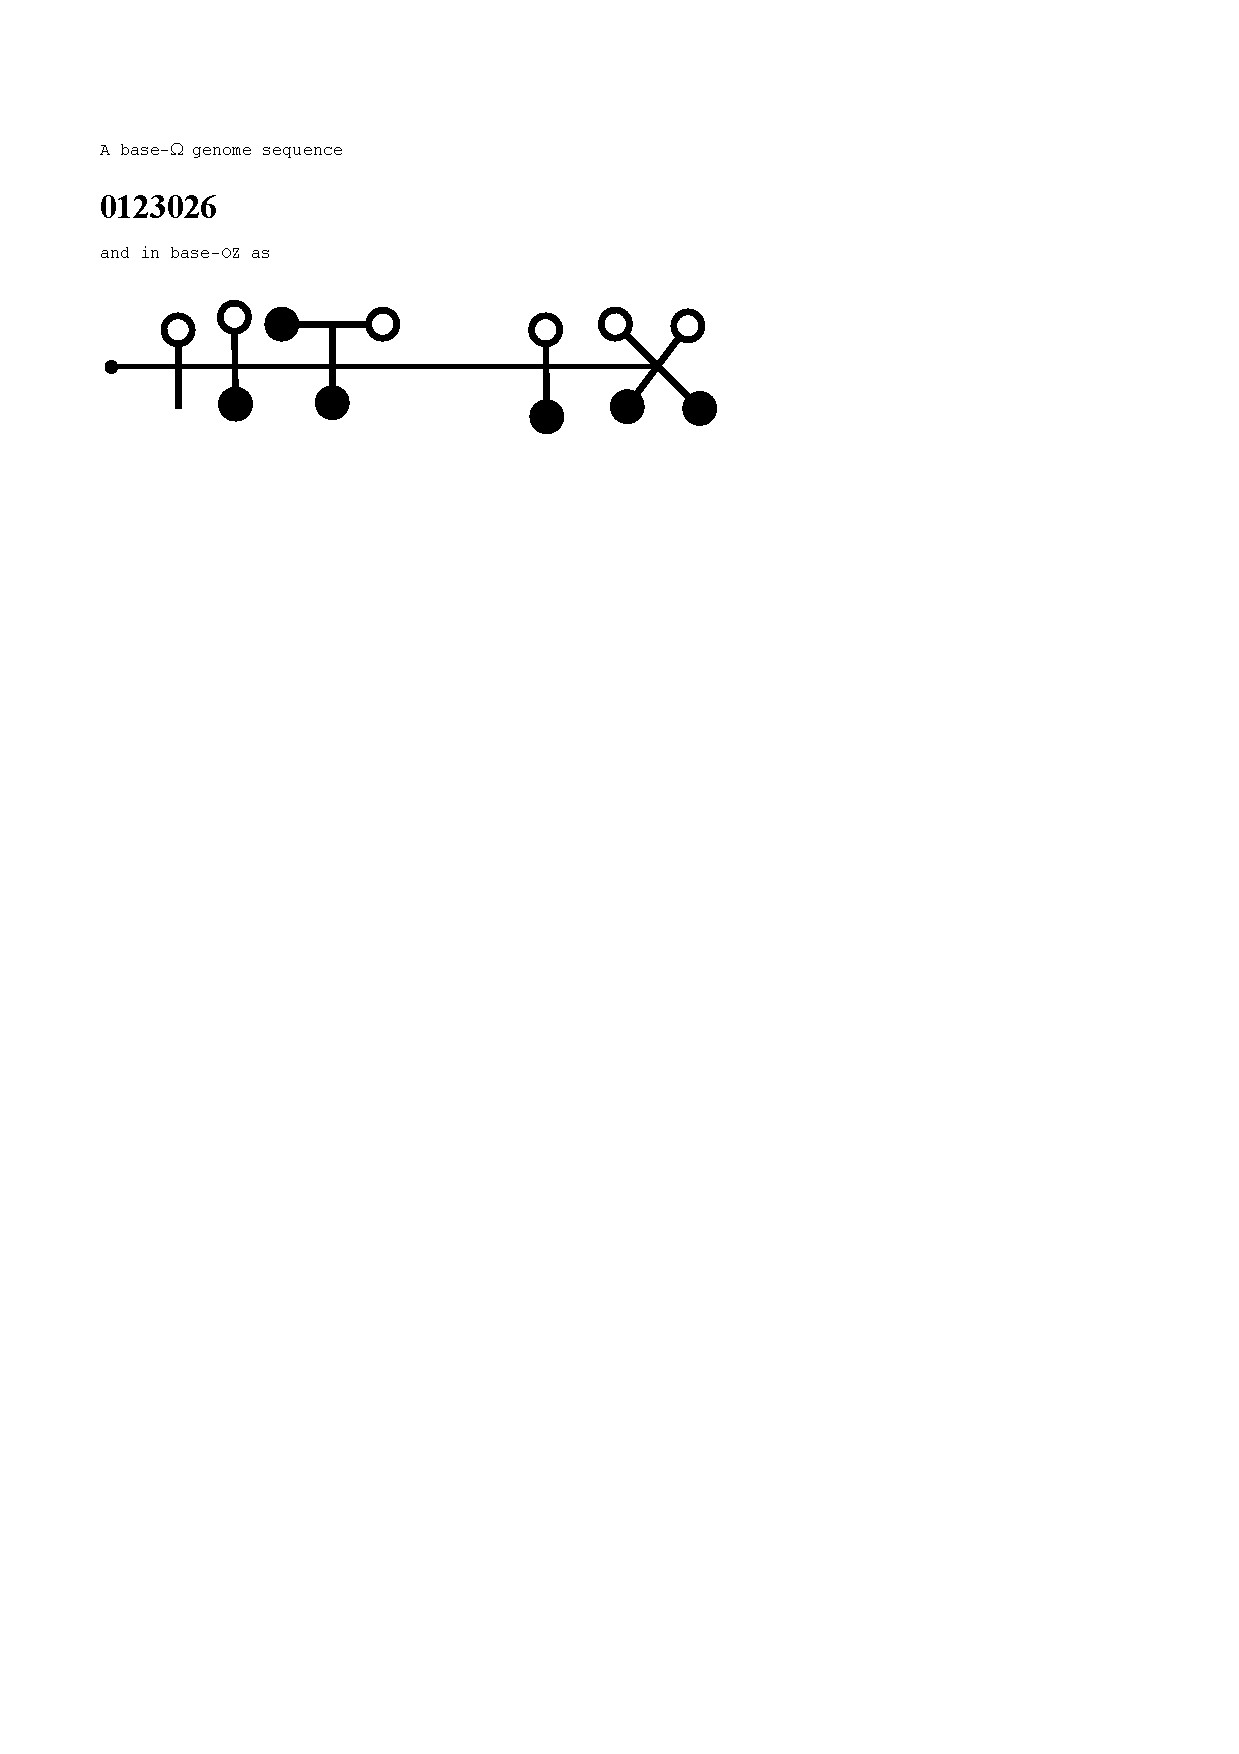
\includegraphics[trim=0cm 20cm 0cm 0cm, clip, width=0.9\textwidth,]{resources/pdfs/OZINCIPHER-APP3-EXA.pdf}\\
   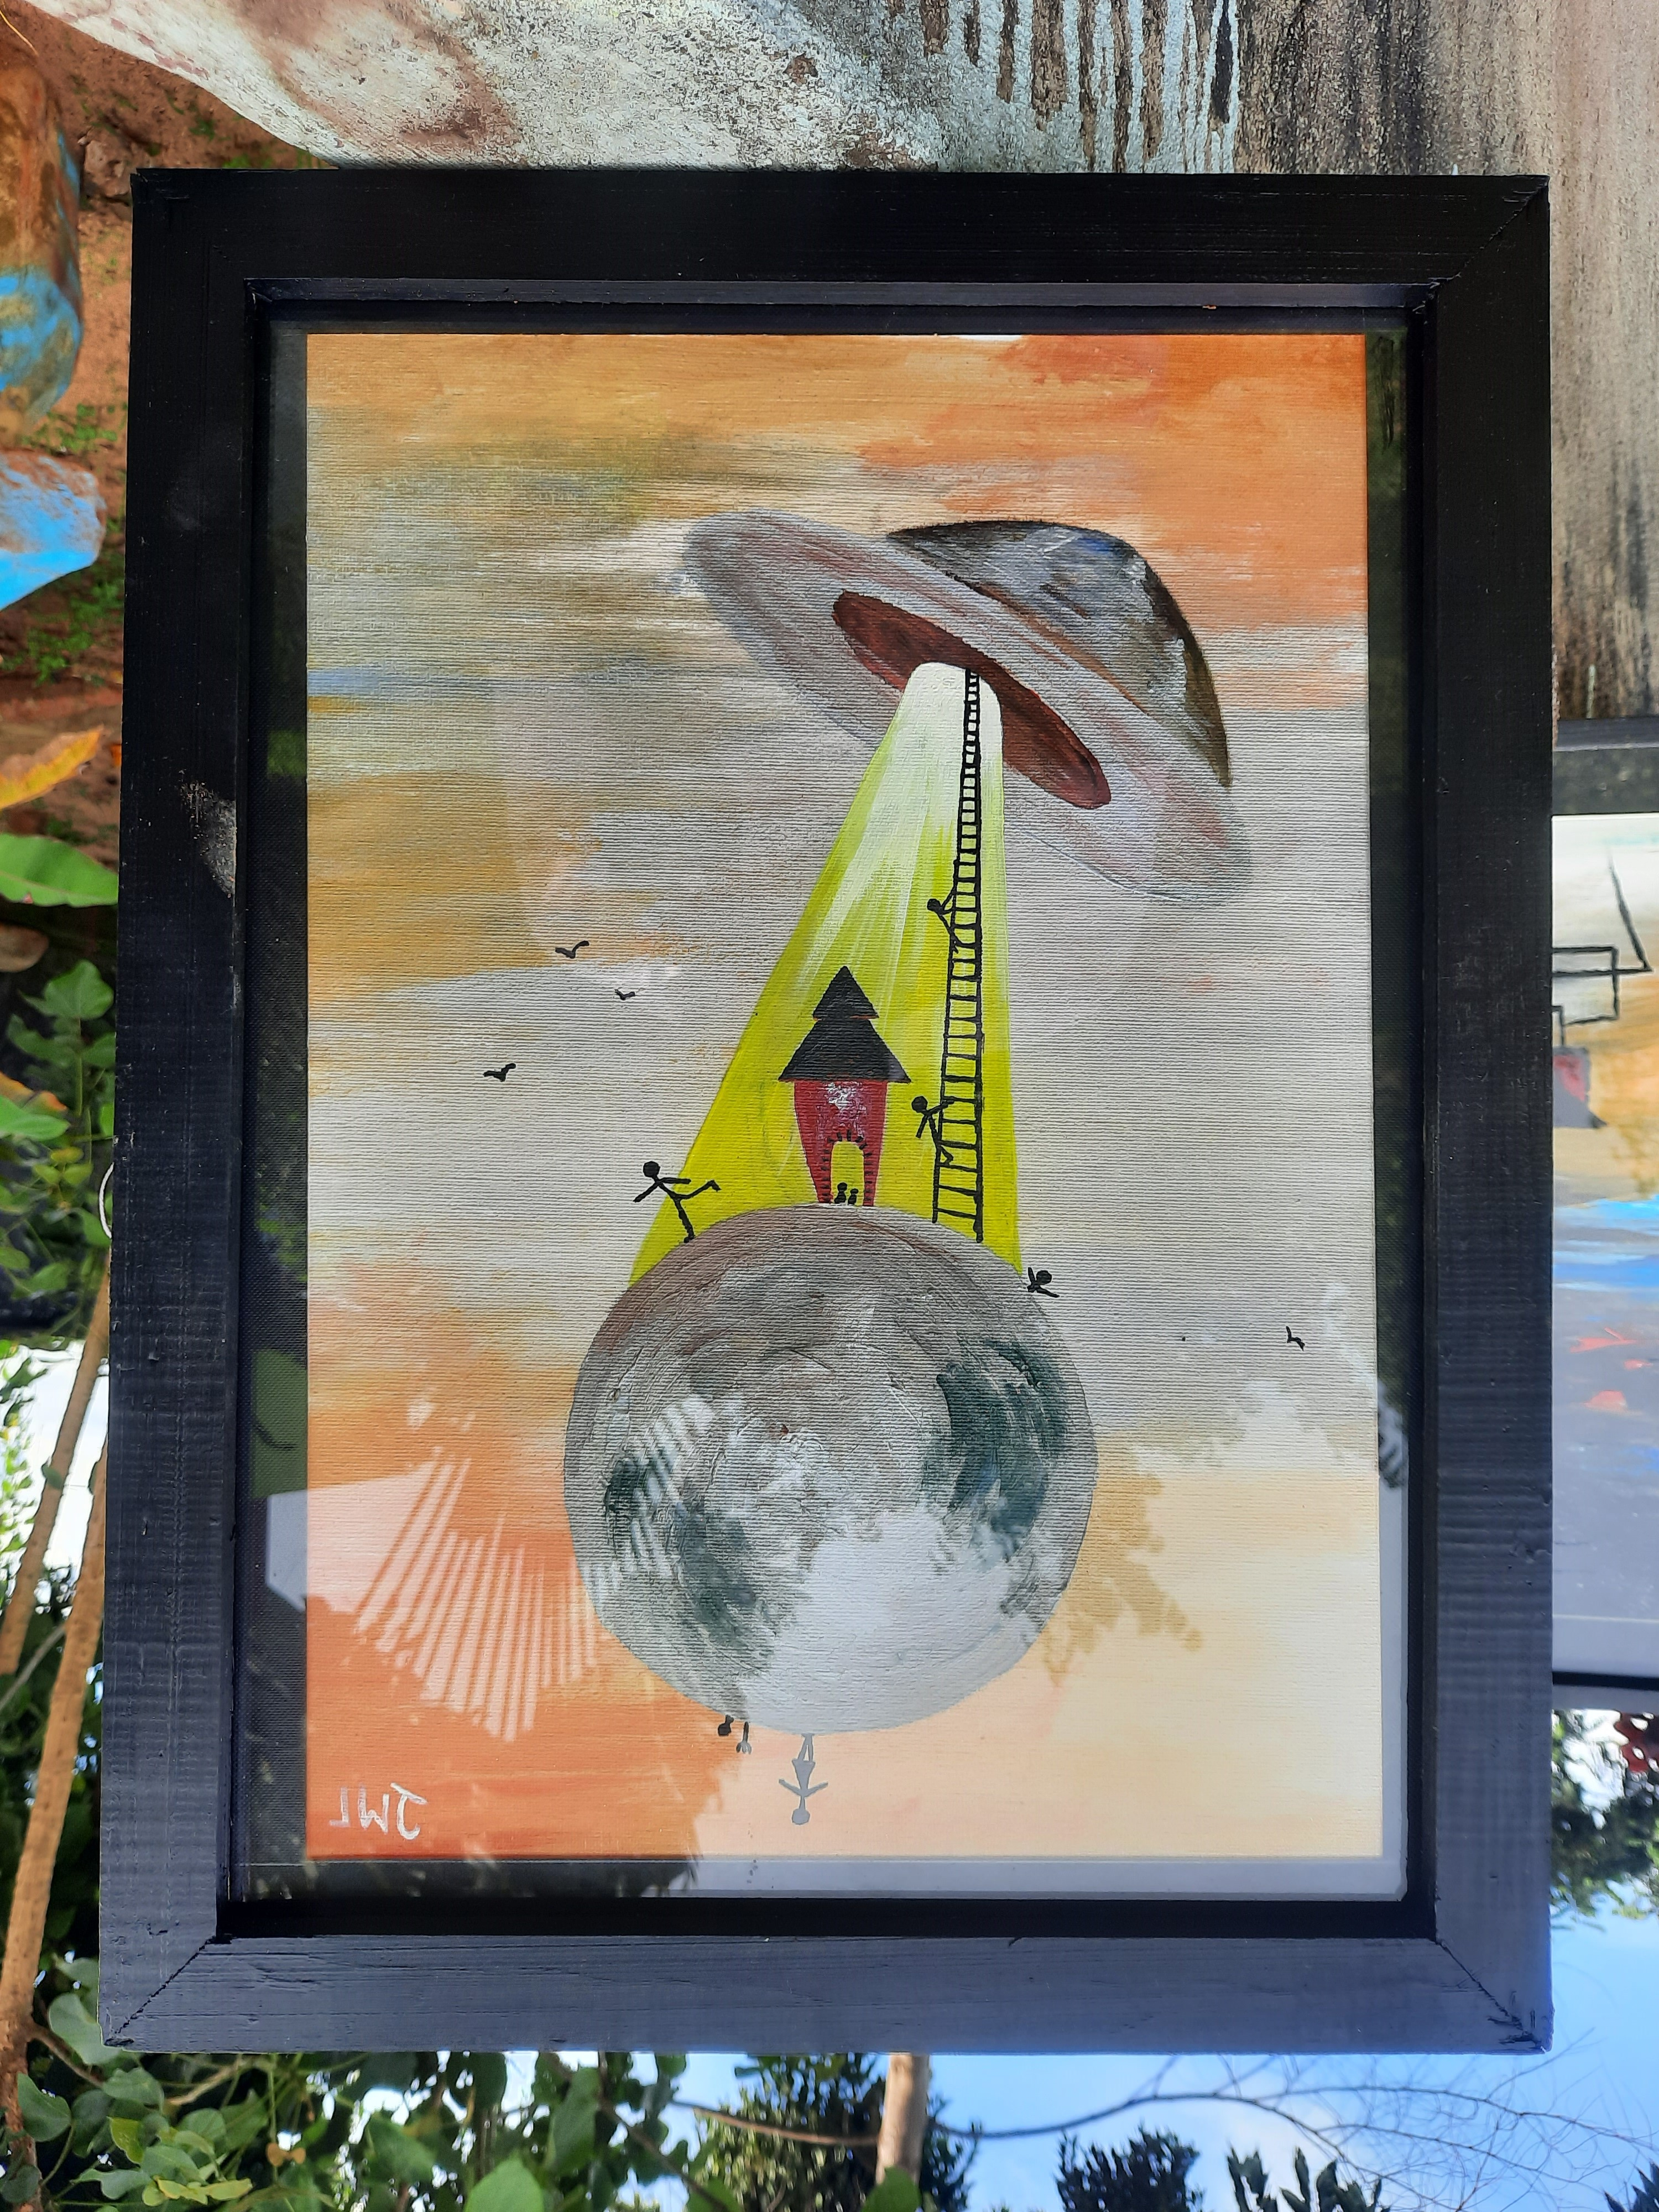
\includegraphics[trim=0cm 0cm 0cm 0cm, clip, width=0.9\textwidth,]{resources/images/annunaki.jpg}\\
   \caption{The surreal painting, ``Arrival of the Anunnaki", by Joseph W. Lutalo, as part of their 2022 \textbf{The Zermelo Frankael Dream Collection} that was first exhibited at Ndugu Art Gallery then in Entebbe Town.}
  \label{FIGANNUNAKI}
  \end{center}
\end{figure}


\begin{center}
\fbox{
\begin{minipage}{\textwidth}


\texttt{In a dream, I have seen that I was somewhere in a laboratory with some very intelligent fellows and that we were exploring potential applications of TRANSFORMATICS in PHYSICS, by conducting simulation experiments using a large hologram machine that looked like a table around which we sat and held discussions.}

\texttt{I saw that among interesting analyses we conducted was the matter of trying to understand ``The Bermuda Triangle Problem". In particular, we were simulating a strong magnetic field situated at the center of some location upon earth, and that if any flying object --- such as Flying Saucers (UFOs) attempted to fly close enough to this gravitating point, it would cause their trajectories to somewhat get warped towards the center, and so that, no matter how strong the tangential velocity of the craft was relative to the center of attraction at some moment with time T=tn, at any other later moment such as T=t(n+1), the centripetal force on the craft would be even stronger, and that the distance from the point of the center of attraction would be lesser at t(n+1) than at tn, and so that, eventually the craft would spiral down into the point and somewhat crash or (like for the case of the whirlpool-like Bermuda Triangle), get swallowed into some kind of black hole (in the ocean).}

\texttt{The simulations looked so realistic despite being generated by a super computer, and it felt like we were performing reconnaissance studies about aliens visiting Earth at say... Area 51! Then I woke up.
}


\#\#\# \textbf{A Dream About The Bermuda Triangle Experiment \& Applying TRANSFORMATICS in PHYSICS}

\end{minipage}}
\\
\end{center}

\large

\textbf{NOTE:} \textit{After waking up and thinking a bit about all this.. a stunning realization occurred to me; there's an acrylic painting I once did (titled ``Arrival of the Annunaki", and which I had exhibited at the then Ndugu Art Gallery in Entebbe Town circa 2022, but which now was at home with me), in which I painted a vision that had occurred to me concerning a spaceship that visited Earth some day (in the future perhaps), and that the ship shone a very brilliant light upon some village, and that as people freaked out, a ladder descended from the ship onto the earth, and some few bold people ascended into the ship by climbing up that ladder, while others, too afraid, only scattered and ran away.} 


\textit{So, while thinking about this Bermuda experiment on TRANSFORMATICS and also this interesting painting, and trying to connect the dots... I feel like.. perhaps there is something about the DNA ladder-like structure that could get us to understanding the biology or natural powers of aliens? Life on other planets or worlds perhaps? Jacob's ladder from the Scriptures perhaps? Basically, it strongly feels like these two ``dreams" might be telling us (or me in particular) or pointing us towards something both alarming and exhilarating! Also, it could indeed inspire future directions and explorations of TRANSFORMATICS in both PHYSICS and GENETICS!}


\textit{\#dream \#diary \#advanced \#physics \#transformatics \#jwl \#reflections \#futuredirections
\#CREATED:Aug 22, 2025 03:02:32}

\Large

%-------[ END CONTENT ]


\end{appendices}

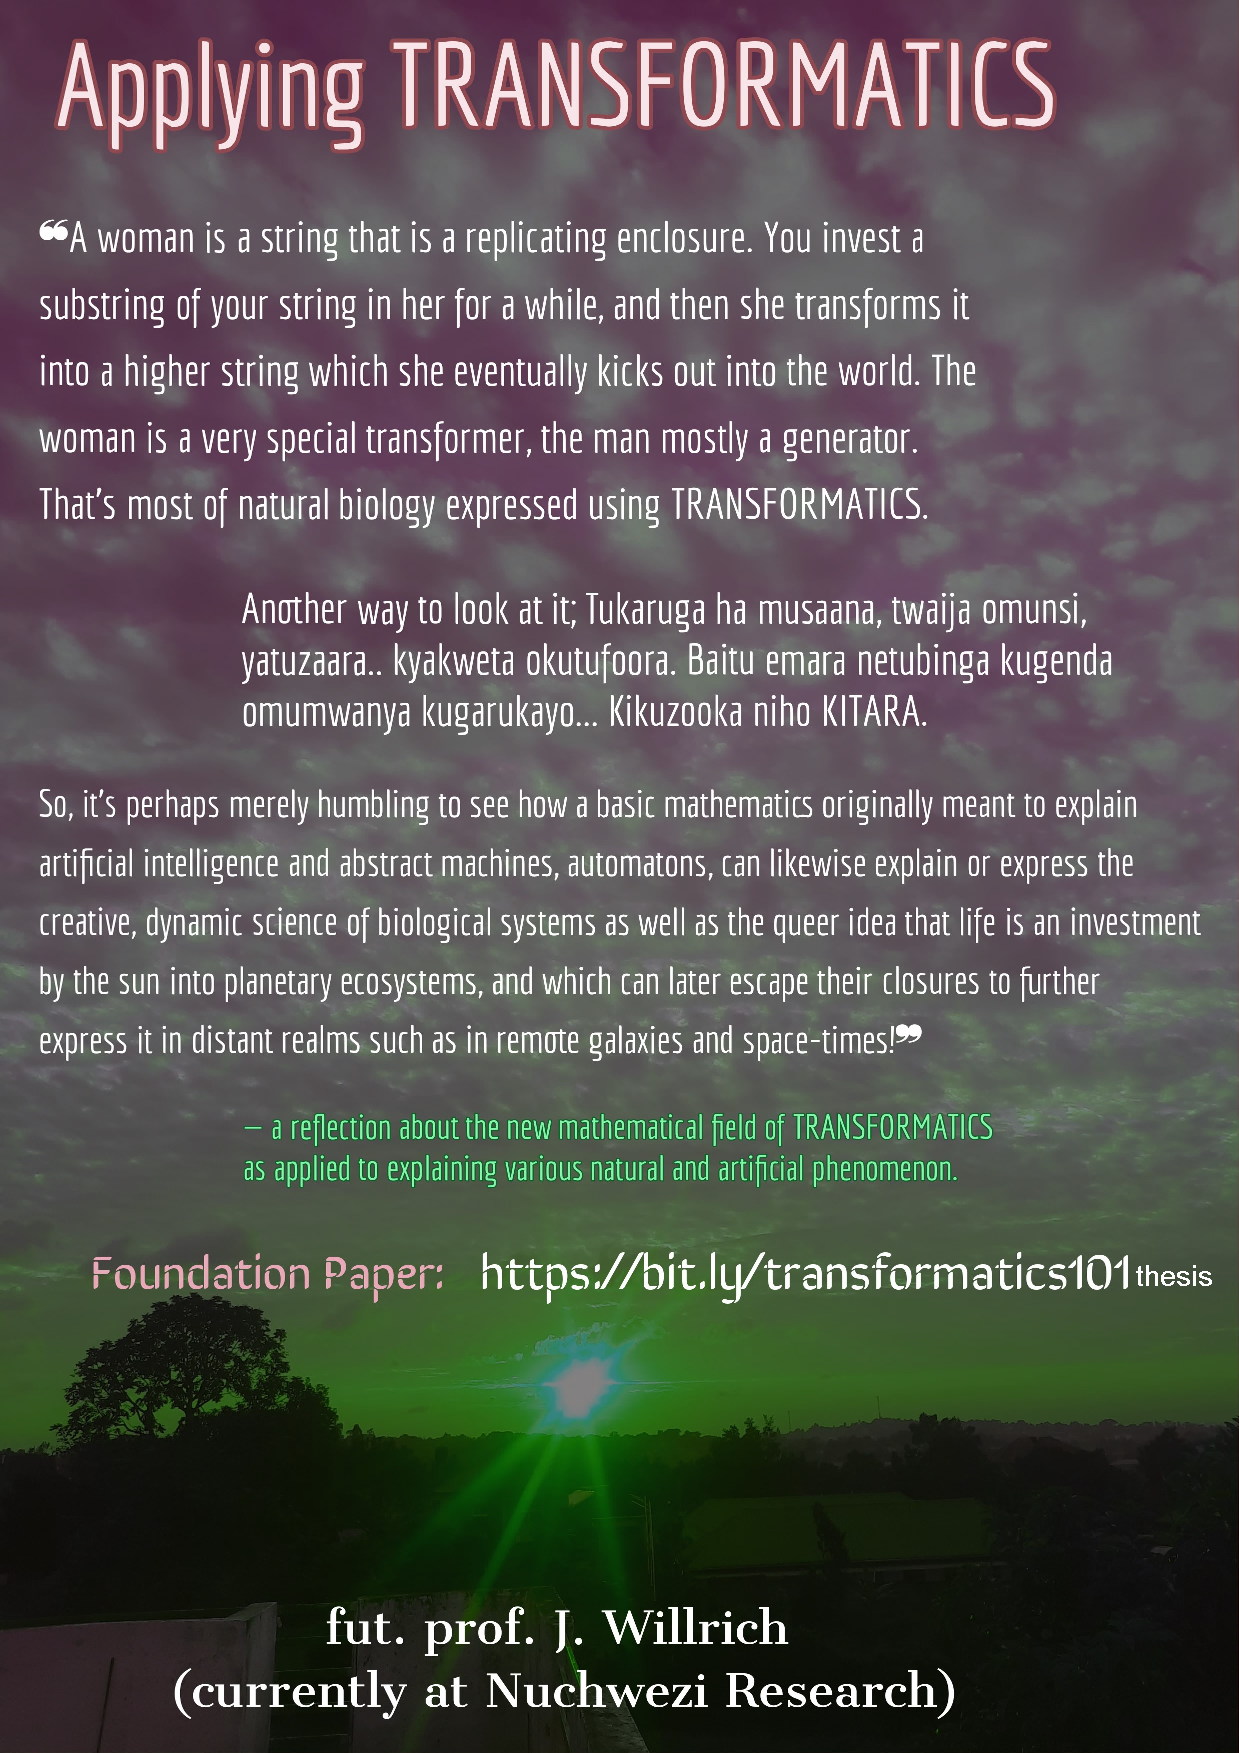
\includepdf[pages=1]{resources/pdfs/note_cover.pdf}

\bibliographystyle{unsrt}
\bibliography{references}

%\comment{

%\newpage

\vspace{5cm}
\fbox{
\begin{minipage}{0.9\textwidth}
\textbf{TO CITE:}\\

Lutalo, Joseph Willrich (2025). \textbf{Applying TRANSFORMATICS in GENETICS} I*POW. Books. \url{https://www.academia.edu/143516392/}

\end{minipage}}
\\
%}


%---[ END BOOK END/BACKCOVER]


\chapter*{Final Dedication}
\addcontentsline{toc}{chapter}{Final Dedication}


\begin{table}[H]
  \centering
  \Huge
	\begin{tabular}[t]{|p{0.65\textwidth}}
$   ``$ \textbf{With}\textit{out having to print their actual \textbf{na-Sequences} here...    \Large This work is additionally dedicated to all \st{my} kids, especially  \textbf{Arora J. Muntu}, currently only 2, a jolly, explorative fellow.} If not especially for them, perhaps this \textbf{book would not have advanced past the front cover.}\\
	\hline
	              
\end{tabular}
  \label{TABFINDEDC}
\end{table}


% Float the section to center of page
\begin{center}
\vspace*{\fill}

\chapter*{About the Author\footnote{Refer to \textbf{ORCID:} \url{https://orcid.org/0000-0002-0002-4657}}}
\addcontentsline{toc}{chapter}{About the Author}


\begin{figure}[H]
  \begin{center}
  %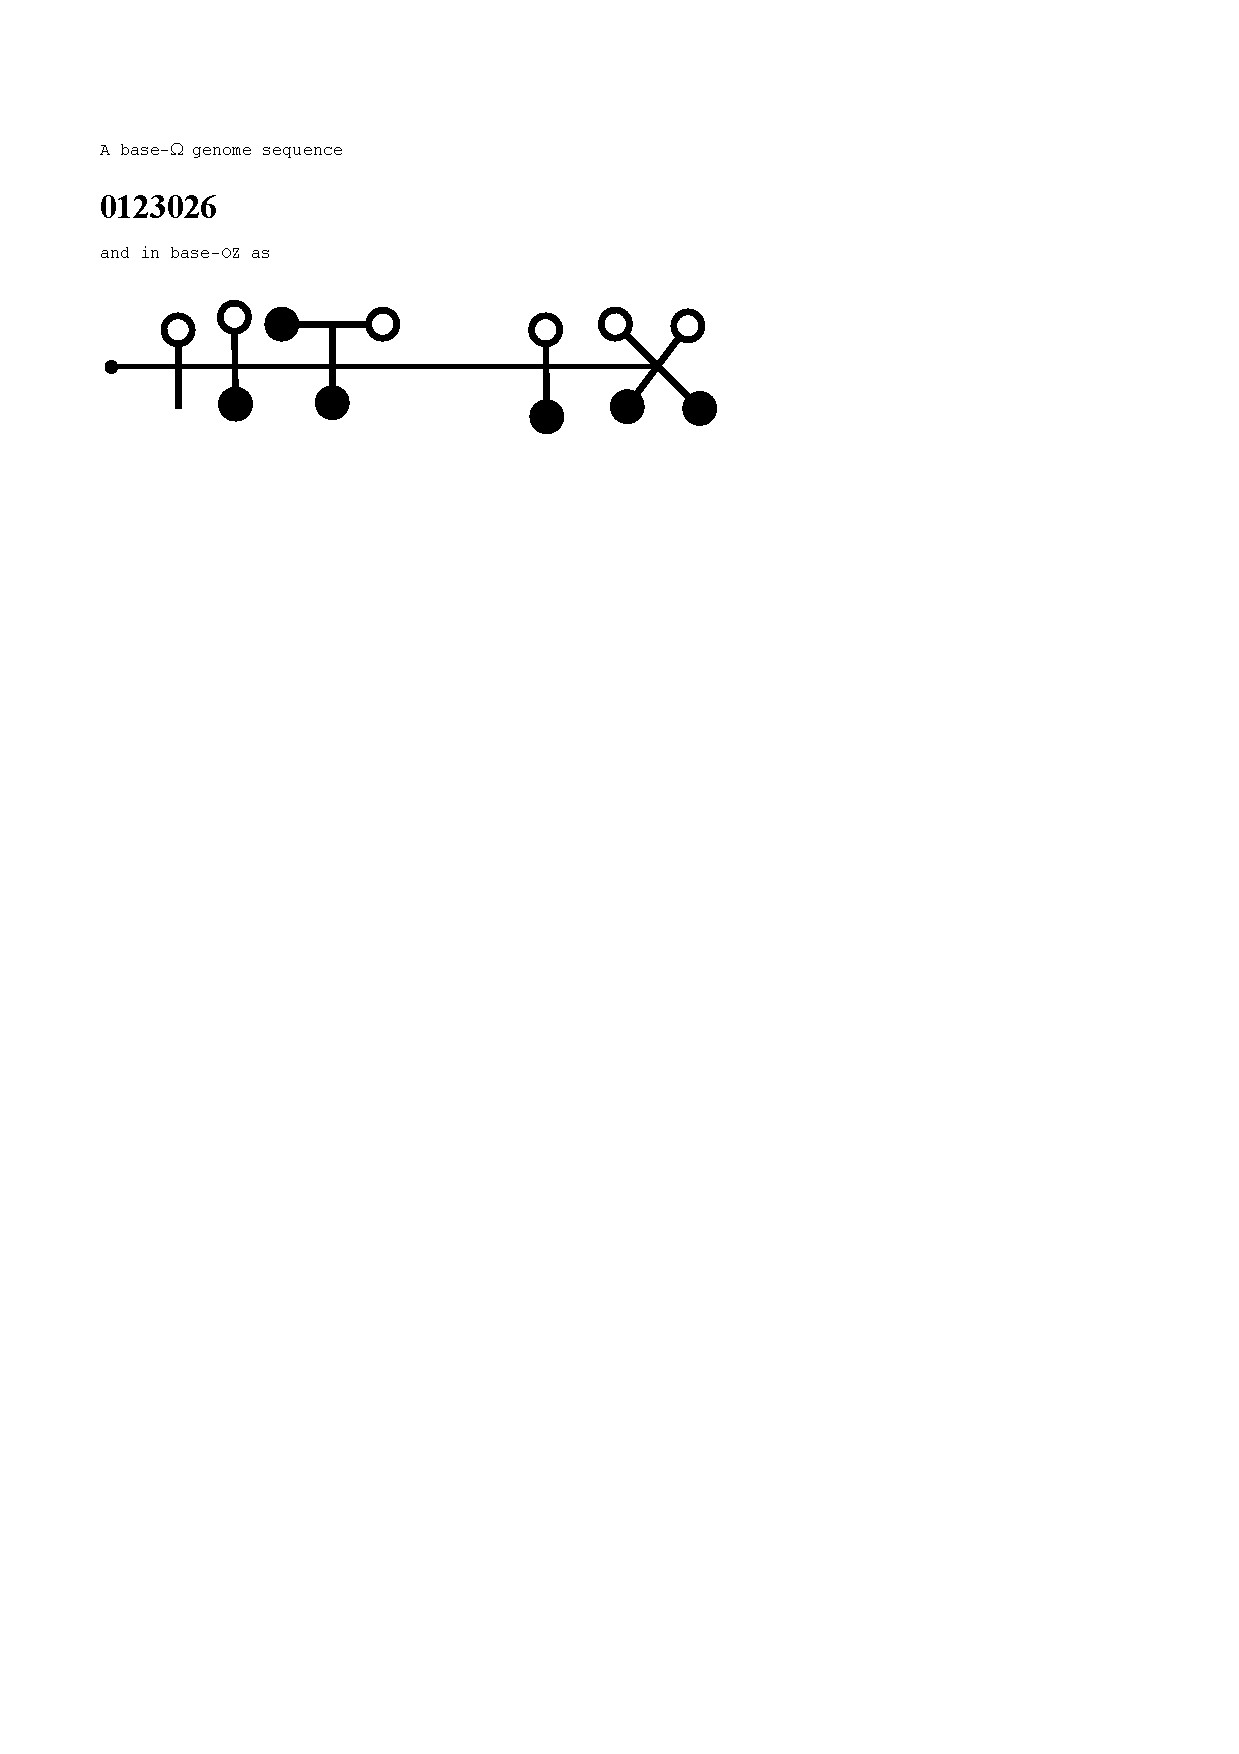
\includegraphics[trim=0cm 20cm 0cm 0cm, clip, width=0.9\textwidth,]{resources/pdfs/OZINCIPHER-APP3-EXA.pdf}\\
  %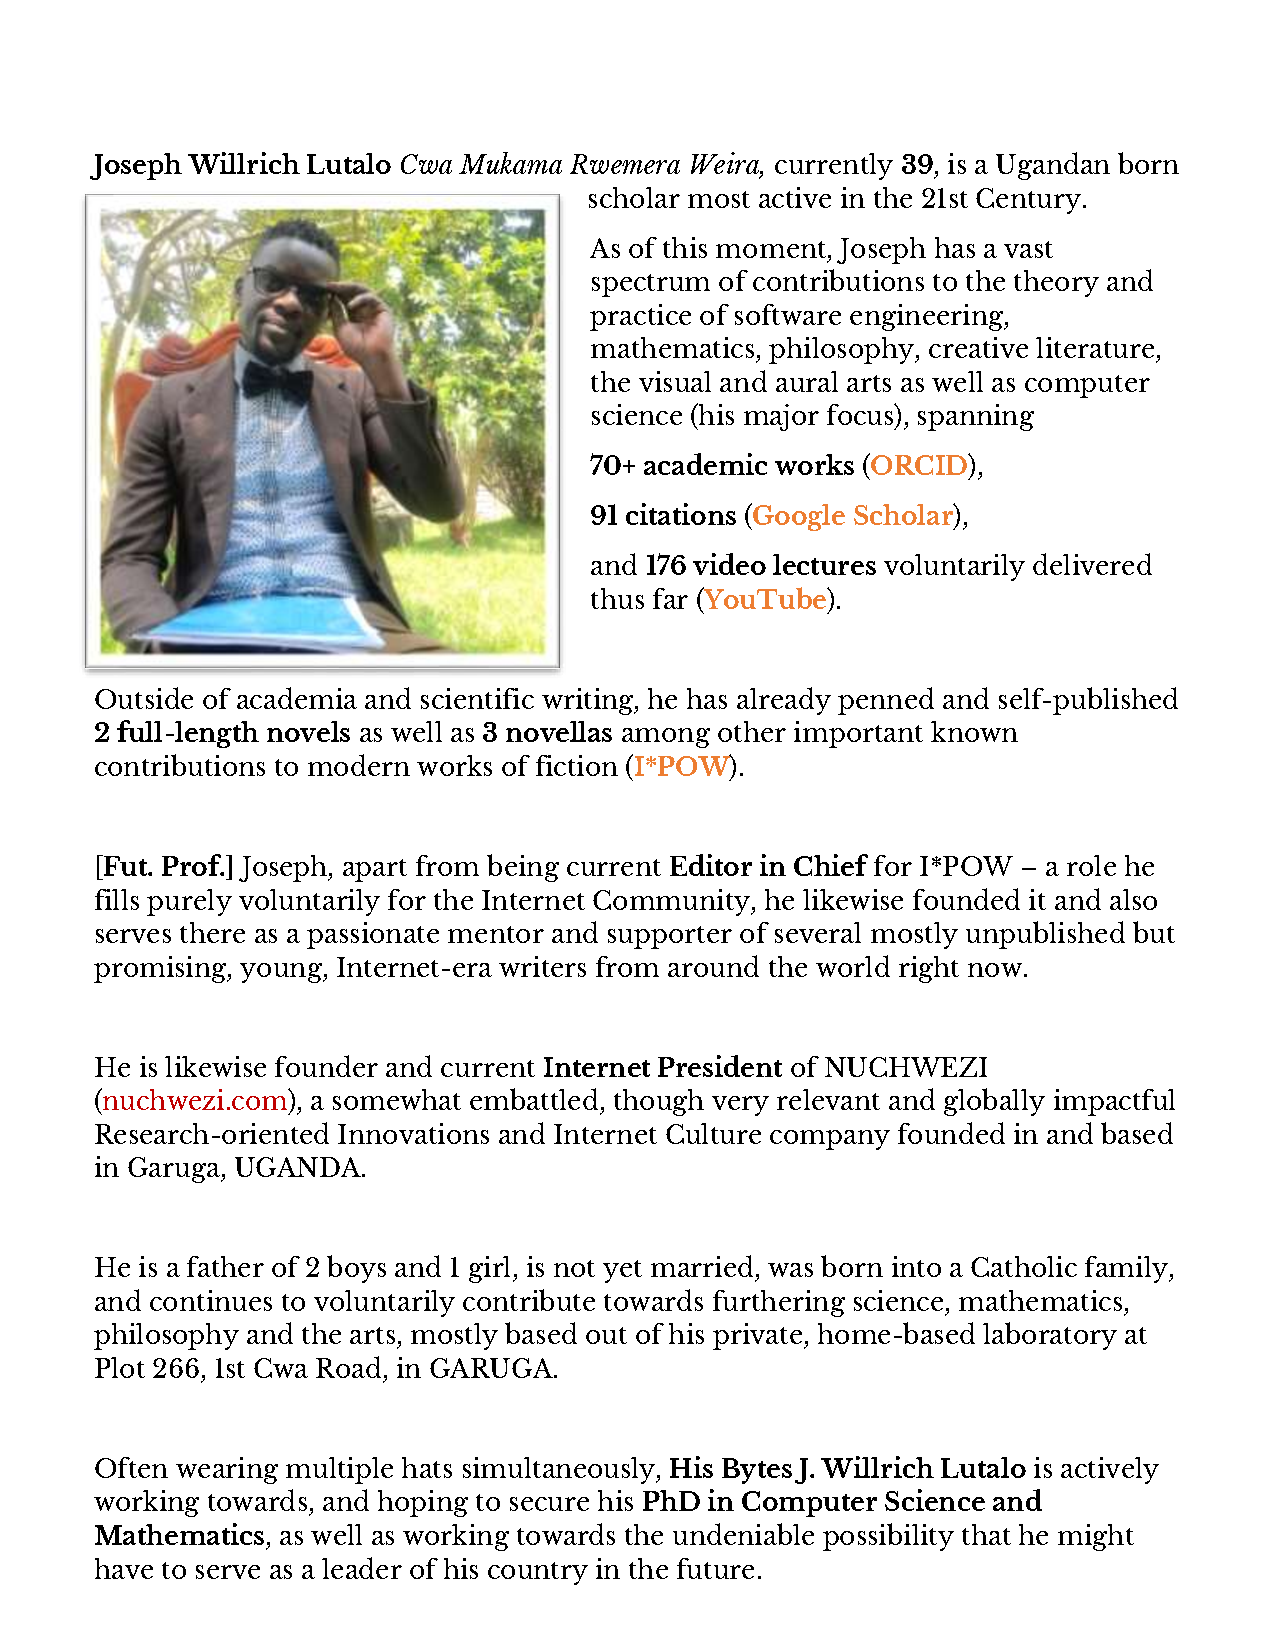
\includegraphics[trim=LEFT BOTTOM RIGHT TOP, 
   \includegraphics[trim=0cm 1cm 0cm 2cm, clip, height=0.8\textheight,]{resources/pdfs/AboutAuthor.pdf}\\
   %\caption{The \textbf{alternative rendering}  of the same sequence as $\Omega_{veuler}$.}
  %\label{FIGLGESEULERVIRUSv2_ORIG}
  \end{center}
\end{figure}

\vspace*{\fill}
\end{center}


\chapter*{Index}
\label{CHAPINDEX}
\printindex


\chapter*{Colophon}
\addcontentsline{toc}{chapter}{Colophon}


\texttt{COVER-ART:} \textbf{J. Willrich Lutalo}, as prompt engineer, using \textbf{Microsoft Bing Image Creator}, powered by DALL$-$E.


\texttt{GRAPHICS:} \textbf{Adobe Express} on Android.


\texttt{PRIMARY-EDITOR:} \textbf{TexMaker} v6.0.0 using \textbf{LaTeX} on Microsoft Windows v10.


\texttt{REFERENCE-MANAGER:} \textbf{BibTeX} v0.99d (package manager: MiKTeX v24.4).


\texttt{SECONDARY-EDITOR:} \textbf{VIM}, Vi IMproved v8.2 text editor, via \textbf{WSL}.


\texttt{PUBLISHER:} \textbf{I*POW} \url{https://t.me/ipowriters}


\texttt{FONT:} \textbf{Computer Modern Roman}

% insert [back] cover --- could just be a PNG or PDF
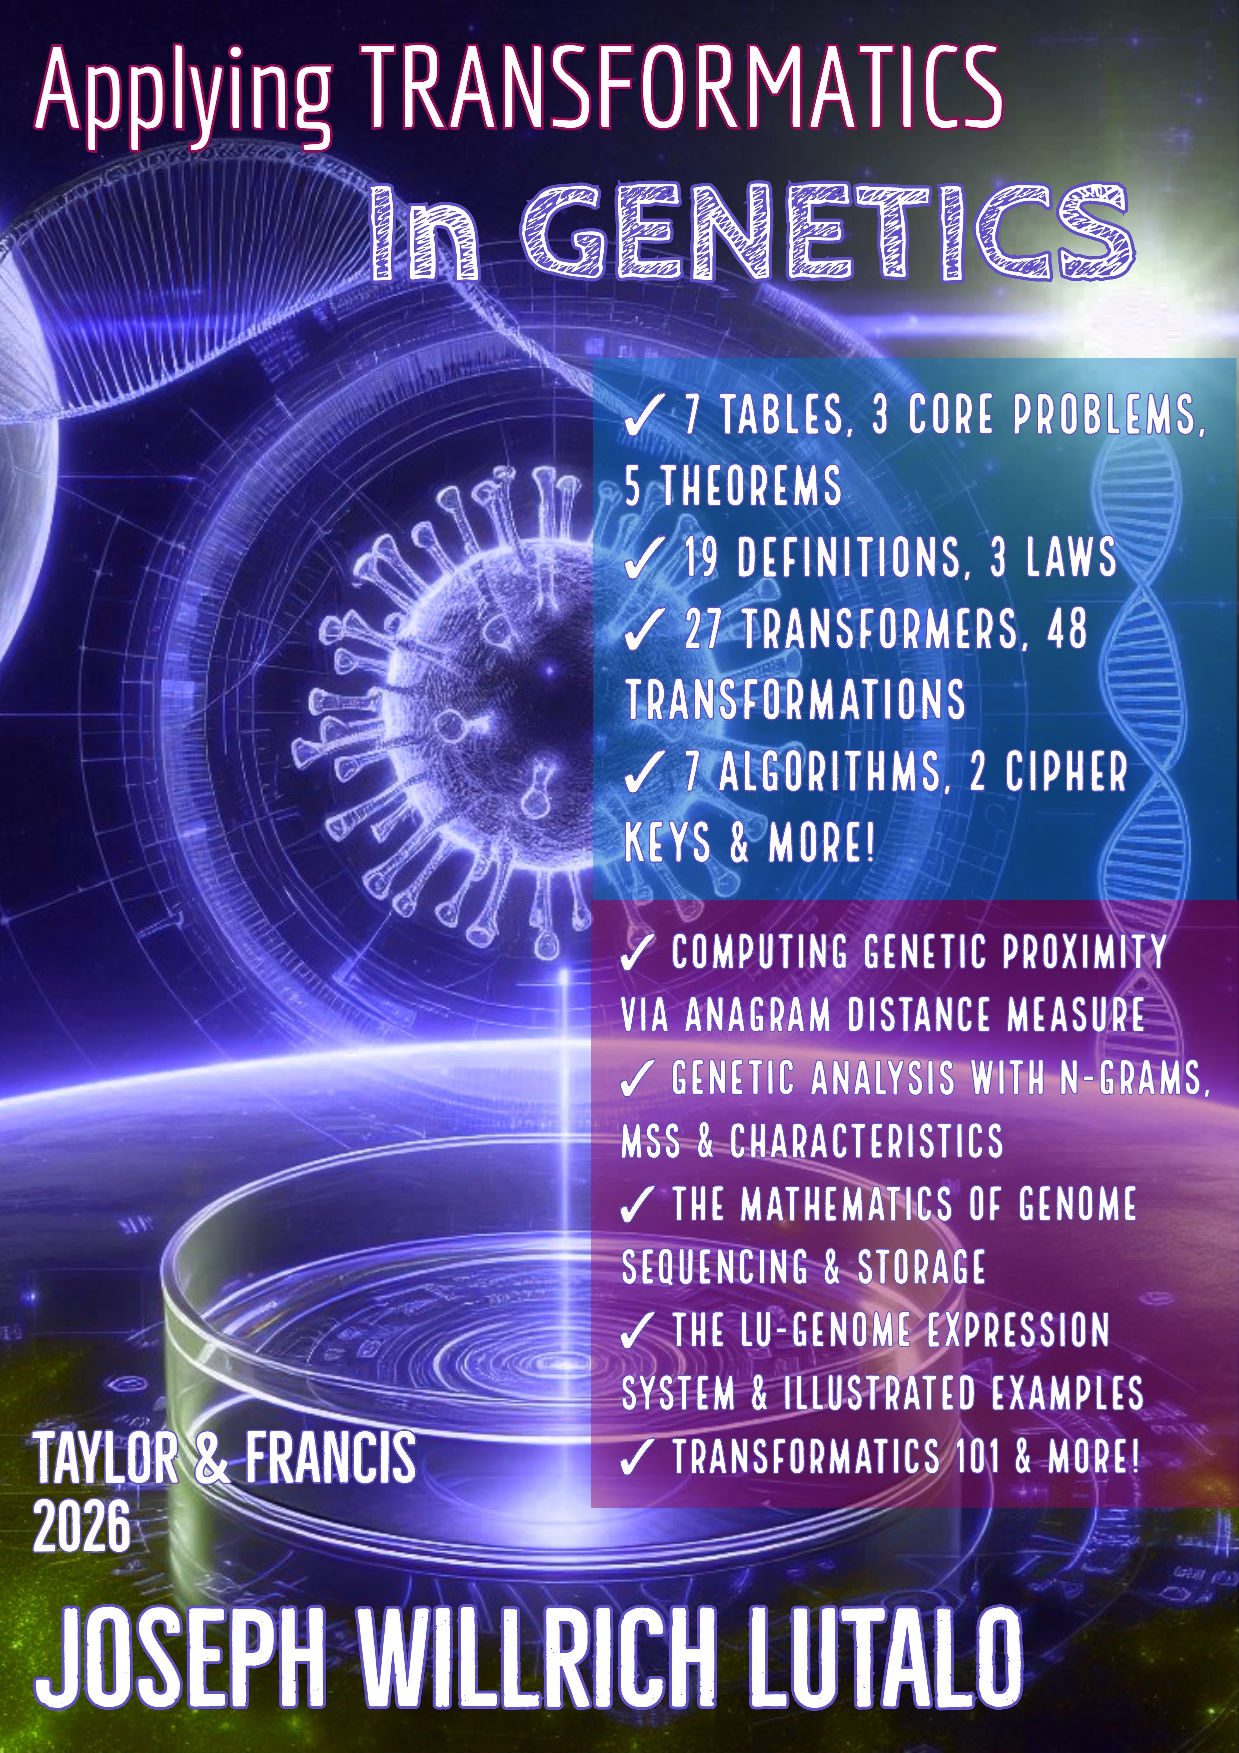
\includepdf[pages=1]{resources/pdfs/back_cover.pdf}

\end{document}
